\documentclass{book}
\usepackage[utf8]{inputenc}
\usepackage{framed}
\usepackage{epigraph}
\usepackage{multirow}
\usepackage{amssymb}
\usepackage{listings}   
\usepackage{amsmath}
\usepackage[numbers]{natbib}
\usepackage{blkarray}
\usepackage[pdftex]{graphicx} 
\usepackage{multicol}
\usepackage[ruled,vlined,linesnumbered]{algorithm2e}
\usepackage{csquotes}
\usepackage{booktabs}
\newtheorem{theorem}{Theorem}
\newtheorem{defn}{Definition}[chapter]
\usepackage{environ}
\NewEnviron{myequation}{%
\begin{equation}
\scalebox{1.5}{$\BODY$}
\end{equation}
}
\usepackage{color}

\definecolor{mygreen}{rgb}{0,0.6,0}

\definecolor{mygray}{rgb}{0.5,0.5,0.5}
\definecolor{mymauve}{rgb}{0.58,0,0.82}

\lstset{ %
  backgroundcolor=\color{white},   % choose the background color; you must add \usepackage{color} or \usepackage{xcolor}
  basicstyle=\footnotesize,        % the size of the fonts that are used for the code
  breakatwhitespace=false,         % sets if automatic breaks should only happen at whitespace
  breaklines=true,                 % sets automatic line breaking
  captionpos=b,                    % sets the caption-position to bottom
  commentstyle=\color{mygreen},    % comment style
  deletekeywords={...},            % if you want to delete keywords from the given language
  escapeinside={\%*}{*)},          % if you want to add LaTeX within your code
  extendedchars=true,              % lets you use non-ASCII characters; for 8-bits encodings only, does not work with UTF-8
  frame=single,	                   % adds a frame around the code
  keepspaces=true,                 % keeps spaces in text, useful for keeping indentation of code (possibly needs columns=flexible)
  keywordstyle=\color{blue},       % keyword style
  language=Octave,                 % the language of the code
  otherkeywords={*,...},           % if you want to add more keywords to the set
  numbers=left,                    % where to put the line-numbers; possible values are (none, left, right)
  numbersep=5pt,                   % how far the line-numbers are from the code
  numberstyle=\tiny\color{mygray}, % the style that is used for the line-numbers
  rulecolor=\color{black},         % if not set, the frame-color may be changed on line-breaks within not-black text (e.g. comments (green here))
  showspaces=false,                % show spaces everywhere adding particular underscores; it overrides 'showstringspaces'
  showstringspaces=false,          % underline spaces within strings only
  showtabs=false,                  % show tabs within strings adding particular underscores
  stepnumber=2,                    % the step between two line-numbers. If it's 1, each line will be numbered
  stringstyle=\color{mymauve},     % string literal style
  tabsize=2,	                   % sets default tabsize to 2 spaces
  title=\lstname                   % show the filename of files included with \lstinputlisting; also try caption instead of title
}


\title{75.06, 95.58 Organización de Datos\\Apunte del Curso}
\author{Luis Argerich, Natalia Golmar, Damián Martinelli, Martín Ramos Mejía,\\
 Juan Andrés Laura.\\
  Universidad de Buenos Aires\\
  Facultad de Ingenieria}
\date{\today\\v2.0}


\begin{document}
\frontmatter      
\maketitle        
\tableofcontents  

\mainmatter        

\part{Data Science}

\chapter{Fundamentos}

\epigraph{Sometimes beginnings aren't so simple}{\textit{The Shadow of the Day \\ Linkin Park}}

\section{Introducción}
Data Science es la rama de la computación que se encarga de entender, procesar y extraer valor a partir de los datos. Hoy en día existen innumerables fuentes de datos y herramientas para recolectar datos, desde el log de un website hasta la estructura de una Red Social pasando por bases de datos en todo tipo de formatos y pertenecientes a los mas diversos dominios. 

Una forma muy popular de definir Data Science es mediante la intersección de tres áreas: Una que cubre los aspectos matemáticos y estadísticos, otra que cubre la parte computacional, es decir algoritmos y programación y finalmente un área que es propia del dominio en cuestión, es decir conocimiento sobre el tema del cual tratan los datos. 

\begin{figure}[!htb]
\centering
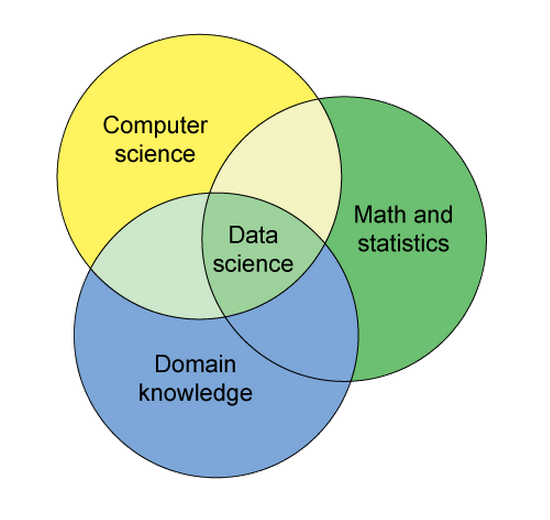
\includegraphics[width=2in]{figures/data-science-fig.png}
\caption{Data Science.}
\label{fig1}

\end{figure}

La aplicación de Data Science a un conjunto de datos puede darse de las mas diversas formas y con diversos objetivos, en general el proceso consiste en obtener a partir de los datos las respuestas que necesitamos a ciertas preguntas que resultan importantes. Podemos generalizar la mayoría de los procesos de Data-Science mediante los siguientes pasos:

\begin{enumerate}
\item Hacer una pregunta interesante
\item Conseguir los datos necesarios
\item Explorar los datos
\item Aplicar a los datos el algoritmo necesario 
\item Comunicar los resultados
\end{enumerate}

Cada uno de estos puntos implica una importante cantidad de trabajo, a continuación intentaremos explicar brevemente cuáles son las actividades típicas para cada paso y lo que cada una de estas actividades implica.

\subsection{Hacer una pregunta interesante}

La pregunta que queremos responder es el inicio de todo proceso de análisis de datos, es lisa y llanamente la información que queremos obtener a partir de los datos. Por ejemplo, podemos tener un conjunto de datos sobre propiedades inmuebles, incluyendo sus características y precios a partir del construiremos un modelo que nos permita tasar automáticamente una propiedad a partir de sus características.

Así como éste podríamos listar una enorme cantidad de problemas que podemos resolver usando Data Science. Como no hay espacio para listar todos los problemas posibles vamos a agruparlos en categorías intentando que cada una de estas categorías sea representativa de una buena cantidad de problemas. Es además una buena forma de presentar terminología que usaremos constantemente a lo largo del curso. Por favor notemos que vamos a presentar estas categorías simplemente desde el punto de vista de qué pregunta podemos hacernos en base a nuestros datos, no vamos a entrar aún en detalles ni terminología propios de cada tipo de problema, los lectores que ya tienen alguna experiencia en estos temas tendrán que esperar a que cada uno de estos temas sea desarrollado en mayor detalle.

\subsubsection{Regresión}

En un problema de regresión queremos predecir el valor de una variable \textit{numérica  y continua}  a partir de un cierto conjunto de datos. En general contamos con un cierto set de entrenamiento en el cual conocemos el valor de la variable que queremos predecir. El objetivo es entonces construir un modelo que nos permita predecir el valor de nuestra variable de decisión a partir de datos nuevos. 

\begin{figure}[!htb]
\centering
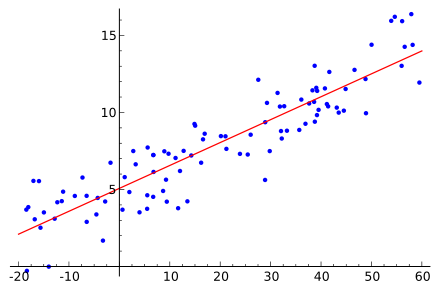
\includegraphics[width=2in]{figures/regression-fig-1.png}
\caption{Regresión lineal.}
\label{fig2}

\end{figure}

El caso mas simple es la regresión lineal en el cual nuestro modelo es una recta, la recta que mejor ajusta a los puntos de nuestro set de entrenamiento. Los problemas de regresión pueden usarse para predecir el valor de las acciones en el mercado de valores, para estimar el costo de una propiedad, para calcular la cantidad de personas en un casino, para estimar las ganancias de un negocio que queremos abrir, etc. Las claves para identificar un problema de regresión son las siguientes:

\begin{itemize}
\item Queremos predecir una variable que es numérica y en general continua
\item Contamos con un set de entrenamiento para el cual conocemos el valor de dicha variable
\end{itemize}

\subsubsection{Clasificación}

La clasificación automática es muy similar a la regresión pero la variable que queremos predecir no es continua sino discreta, frecuentemente tiene pocos valores posibles y en muchos casos los valores posibles son solo dos (clasificación binaria). La idea es la misma que antes, contamos con un set de entrenamiento en el cual para cada dato conocemos la clase a la cual pertenece el mismo, queremos construir un modelo que nos permita clasificar automáticamente datos nuevos cuya clase desconocemos. 

Un caso típico de la clasificación binaria es el análisis de sentimiento, que podría ser una categoría en si misma dada su enorme utilidad. En un problema de análisis de sentimiento queremos saber si un cierto texto es positivo o negativo, es decir si habla bien o mal de un cierto tema. Como set de entrenamiento deberíamos contar entonces con textos para los cuales ya conocemos su sentimiento. Como podrán imaginarse esto tiene muchísimas aplicaciones como por ejemplo analizar si los reviews de un producto son buenos o malos, determinar si un usuario de una Red Social está pasando por un mal momento, medir la actitud del público en general ante determinadas noticias por los comentarios que existen en un medio gráfico, etc. Y ésta es solo una de las muchísimas formas que puede tomar un problema de clasificación.

Otro ejemplo que estudiaremos mas adelante consiste en predecir la clase a la cual pertenece un vino en base a sus propiedades químicas, contamos como set de entrenamiento con un conjunto de vinos para los cuáles conocemos su clase y el valor de ciertas propiedades químicas del mismo y en base a estos datos queremos construir un modelo que nos permita predecir la clase para vinos nuevos cuya clase desconocemos en base a sus propiedades.

Para reconocer un problema de clasificación en general hay que estar atentos a las siguientes pistas:

\begin{itemize}
\item Queremos determinar la clase a la que pertenece cada dato
\item La clase es una variable discreta con un set de valores posibles limitado y definido
\item Contamos con un set de entrenamiento para el cual conocemos los datos y a que clase pertenecen
\end{itemize}

En algunos casos existe una zona gris entre problemas de clasificación y de regresión, como ejemplo planteemos el siguiente problema: Contamos con reviews para un determinado producto, por ejemplo autos y para cada review hay un número de 1 a 5 que indica que tan positivo es el mismo, por ejemplo las típicas estrellitas con las que podemos calificar cosas en varios sitios. Este problema lo podríamos plantear como un problema de clasificación con cinco clases o bien como un problema de regresión con valores posibles del 1 al 5. La diferencia es que en un problema de regresión nuestro modelo podría predecir 3.45 para un cierto review mientras que en un problema de clasificación los valores posibles son solo 1,2,3,4 y 5. No existe una receta para resolver este tipo de situaciones; en algunos casos obtendremos mejores resultados planteando el problema como una regresión y en otros como una clasificación.

Es frecuente plantear un problema de clasificación binaria como un problema de regresión en donde los valores posibles están en el intervalo [0,1]. Esto trae aparejada la ventaja de que los valores que el regresor genera pueden, bajo ciertas circunstancias, interpretarse como la probabilidad de que la observación sea un 1.

\subsubsection{Clustering}

En un problema de clustering contamos con datos que queremos dividir en grupos de forma automática, por ejemplo podemos tener artículos de noticias y querer agruparlos en categorías de forma tal que queden juntos todos los de deportes, economía, política, etc. 

En algunos casos la cantidad de "clusters" la debemos indicar previamente y en otros el algoritmo es capaz de determinarla por si mismo. Otro ejemplo podría ser agrupar películas automáticamente, de forma que queden juntas las que son de un mismo género. 

La detección de comunidades en una red social es un típico problema de clustering en donde los puntos son los usuarios y queremos agruparlos automáticamente en comunidades, de esta forma podemos descubrir grupos de usuarios que tienen un cierto interés en común aun sin saber exactamente cuál es dicho interés.

\begin{figure}[!htb]
\centering
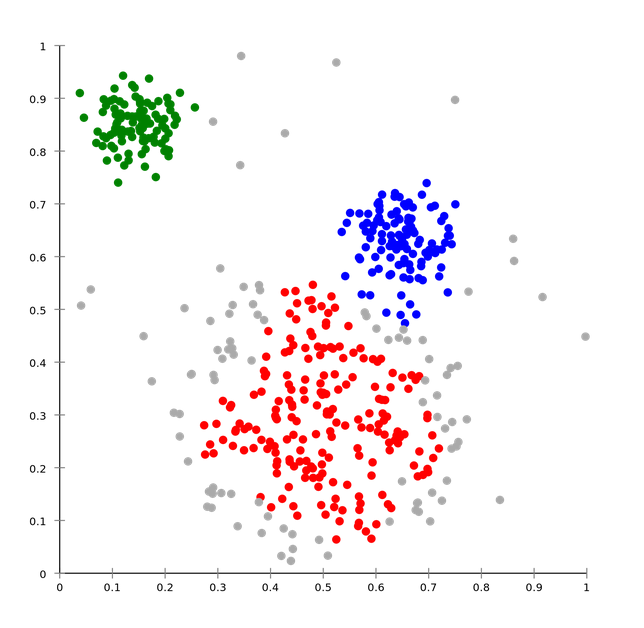
\includegraphics[width=2in]{figures/clustering-fig-1.png}
\caption{Clustering.}
\label{fig3}

\end{figure}

A los problemas de clustering se los suele llamar "aprendizaje no supervisado" en contraste con los problemas de regresión o clasificación que son de tipo supervisado. La diferencia está dada porque no necesitamos conocer el valor de una cierta variable o clase para cada punto, es decir que solo necesitamos los datos en crudo y el algoritmo es capaz de encontrar los clusters automáticamente.


Un problema de clustering se caracteriza, entonces, de la siguiente forma:

\begin{itemize}
\item Contamos con un set de datos
\item Queremos agrupar este set de datos en clusters/grupos/comunidades
\item No son necesarios labels
\end{itemize}

Existe una cierta relación entre los problemas de clustering y de clasificación, por ejemplo dado un problema de clasificación podríamos aplicar clustering primero y luego clasificar a cada punto de acuerdo al cluster al cual pertenece en base a la clase mayoritaria de dicho cluster. Este procedimiento no es muy frecuente pero es conveniente tenerlo en cuenta porque permite entender el funcionamiento de ciertos algoritmos que combinan las propiedades de un problema de clustering y uno de clasificación.

Una aplicación que combina clustering (aprendizaje no supervisado) y clasificación (aprendizaje supervisado) es la que denominamos "Aprendizaje transductivo" en donde usamos los datos para los cuales no conocemos su clase como forma de ayuda a un clasificador tradicional. Consideremos el siguiente ejemplo:

\begin{figure}[!htb]
\centering
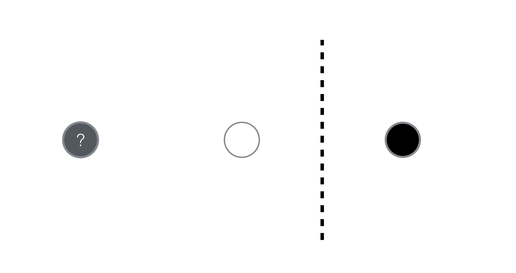
\includegraphics[width=2in]{figures/transduction-fig-1.png}
\caption{Aprendizaje Transductivo.}

\end{figure}

Tenemos solo dos puntos clasificados, uno clasificado como "blanco" y el otro "negro", sin mas información el punto marcado con el signo de pregunta, cuya clase desconocemos, quedaría clasificado como "blanco" ya que está mucho mas cerca del punto blanco que del punto negro.

Veamos ahora que ocurre si agregamos los puntos cuya clase desconocemos:

\begin{figure}[!htb]
\centering
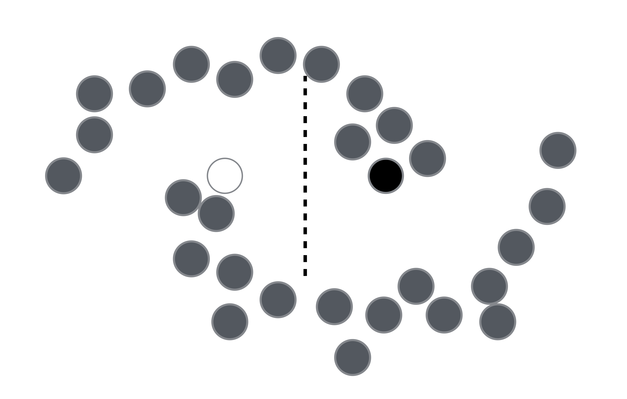
\includegraphics[width=2in]{figures/transduction-fig-2.png}
\caption{Aprendizaje Transductivo.}

\end{figure}

Agregando los puntos sin clase vemos que en nuestros datos existen dos clusters y si tenemos que asociar cada cluster con un color entonces el de "arriba" es negro y el de abajo "blanco" ya que el punto negro pertenece al cluster de arriba y el blanco al de abajo. 

El aprendizaje no-supervisado es una rama muy importante en Data Science ya que solo trabaja con datos sin necesidad de tener un "label" para los mismos, es decir que solo necesitamos los datos en crudo y estos en general son mucho mas fáciles de conseguir que datos ya previamente clasificados.  El aprendizaje transductivo es un área muy nueva dentro de Data Science y que sin dudas merece ser explorada.

\subsubsection{Recomendaciones}

El objetivo de un sistema de recomendaciones es muy simple: recomendarle al usuario cosas que pueden interesarle. El caso mas típico es el de recomendar libros en Amazon, películas en Netflix o productos en un newsletter de un supermercado. También es posible recomendarle a un usuario otros usuarios a seguir en una red social o contenidos que puedan interesarles en un newsreader. 

Los sistemas de recomendación son en general particularmente complejos e involucran el esfuerzo conjunto de varios algoritmos y herramientas, tienen realmente muchos detalles a considerar y por eso vamos a dedicarles un extenso tratamiento mas adelante.

Las características de un Sistema de Recomendaciones son:

\begin{itemize}
\item Tenemos un conjunto de ítems y un conjunto de usuarios
\item Queremos recomendarles a los usuarios ítems que puedan interesarles
\end{itemize}

\subsubsection{Sistemas de Consulta}

Un sistema de consulta es simplemente un buscador, un search engine, el contenido que se almacena puede ser de cualquier formato aunque en general se almacenan páginas HTML o texto plano. El objetivo del sistema de consulta es recuperar los textos o páginas o ítems de información mas relevantes para la consulta planteada por el usuario. Todos estamos familizarizados con este tipo de sistemas ya que son los que definen a los buscadores en la web como Google y otros. 

\begin{figure}[!htb]
\centering
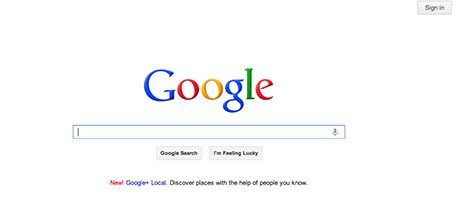
\includegraphics[width=2in]{figures/google-fig.png}
\caption{Un search engine conocido.}
\label{fig4}

\end{figure}
Las características de un sistema de consultas son:
\begin{itemize}
\item Almacenamos información no-estructurada como textos planos, páginas HTML, imágenes, sonido, etc.
\item Queremos encontrar los items de información mas relevantes para las consultas realizadas
\end{itemize}

\subsubsection{Identificación de Patrones}

Este tipo de problemas caracterizan la rama de la computación conocida como \textit{ "Data Mining" }. El objetivo es descubrir información interesante a partir de un conjunto de datos. El ejemplo más clásico es descubrir asociaciones entre los productos que los clientes compran en un comercio, cosas del estilo "el que compra X frecuentemente también compra Y". A esta tarea se la suele llamar \textit{pattern mining}. En muchos casos los algoritmos de pattern mining encuentran asociaciones inusuales o insospechadas, como por ejemplo que quienes compran pañales en un supermercado también suelen comprar cerveza (un ejemplo muy popular en el mundo de Data Science), tal vez esto se deba a que ambas cosas sirven para solucionar el llanto.

Las características de un sistema de identificación de patrones son:

\begin{itemize}
\item Contamos con información que frecuentemente es de tipo transaccional (compras, ventas, visitas a una página, etc)
\item Queremos encontrar patrones, asociaciones entre los ítems que se incluyen dentro de cada transacción
\end{itemize}

Reconocer el tipo de problema que tenemos es sumamente importante ya que nos permite determinar cuales son las armas con las que contamos, es decir los algoritmos que en general suelen funcionar muy bien para problemas similares al que queremos resolver. 

\subsection{Conseguir los datos necesarios}

Conseguir los datos necesarios es un paso fundamental de cualquier proceso de Data Science, en general es la parte que mayor cantidad de tiempo y esfuerzo insume y lamentablemente no suele ser la tarea mas divertida y gratificante.
Conseguir los datos no solo pasa por hacerse de la información que necesitamos sino también depurarla y transformarla en el formato que necesitamos para nuestra tarea. Algunos de los puntos clave en la tarea de recolección de los datos son los siguientes:

\subsubsection{Obtener los Datos}

En esta fase el objetivo es obtener los datos en crudo, en muchos casos esto implica la creación de programas especiales para la captura de los mismos, en otros casos los datos ya están disponibles en una base de datos o en algún formato de archivo. Un detalle importante en esta fase es que en muchos problemas necesitamos un set de entrenamiento y en muchos casos no lo tenemos. Por ejemplo podemos necesitar la calificación de películas para un sistema de recomendaciones o el sentimiento de una buena cantidad de reviews para un sistema de análisis de sentimiento. Lo notable en estos casos es que no es posible automatizar la creación de los \textit{labels} para los datos ya que esto es precisamente lo que pretendemos lograr. Es necesario entonces contar con intervención manual pidiendo a un grupo de humanos que se encargue de crear los labels que necesitamos. Una forma de lograr esto es mediante la contratación del servicio de Amazon conocido como "Mechanical Turk"

\begin{figure}[!htb]
\centering
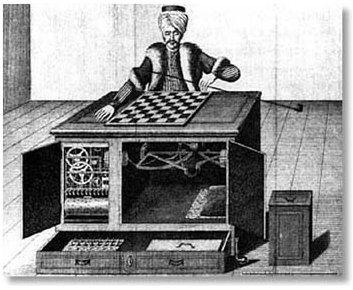
\includegraphics[width=2in]{figures/mechanical-turk-fig.png}
\caption{Mechanical Turk, un androide ajedrecista del siglo XVIII que da origen al nombre del servicio de Amazon.}
\label{fig5}

\end{figure}

En este servicio los usuarios pueden contratar labor humana ofreciendo un cierto precio para realizar tareas repetitivas. Otros usuarios pueden tomar estas tareas y cobrar el dinero ofrecido luego de terminarlas. Esta forma de \textit{crowdsourcing} es muy popular en la comunidad de Data Science en los casos en los cuales es inevitable contar con intervención humana para crear los sets de entrenamiento. Un factor interesante a analizar es si el tipo de comunidad que suele tomar este tipo de trabajos no introduce algún tipo de \textit{bias}\footnote{Por bias se entiende a una tendencia arbitraria que favorece datos de un cierto tipo} indeseado en los datos.

Para la carga de datos de diversas fuentes es necesario contar con un buen conjunto de bibliotecas que permitan leer datos en diversos formatos: SQL, XML, JSON, CSV, TXT, etc.

\subsubsection{Depurar los Datos}

La depuración de datos es frecuentemente la parte que insume mayor tiempo en todo proceso de Data Science, suele ser una tarea bastante tediosa y extensa que prácticamente nadie quiere hacer pero es imprescindible ya que de la calidad de los datos va a depender el éxito de nuestra tarea.
Depurar los datos implica dejarle a nuestros programas datos que son correctos sintáctica y semánticamente. Los errores a corregir son de todo tipo como por ejemplo: formateo de fechas y formatos numéricos, corrección de caracteres inválidos en strings, conversión de tipos, identificación y solución de valores nulos o faltantes, etc.

Mas allá de la corrección del \textit{valor} de cada dato es necesario también asegurarse que los datos estén \textit{Bien Formados},es decir que cada "fila" sea una observación y que cada "columna" sea un atributo. Frecuentemente los datos llegan en formatos que no están bien formados y es necesario realizar algunas manipulaciones para transformarlos.

Veamos algunos ejemplos de datos que no están bien formados y la forma de corregirlos.

\textbf{Ejemplo 1} Nuestro primer ejemplo muestra las notas que los alumnos obtuvieron en ciertas materias:

\begin{table}[!hbt]
\center{
\begin{tabular}{|c|c|c|}\hline
Alumno & 7506 & 7507 \\ \hline\hline
Juan Perez & 7 & 9 \\
Diego Ramirez & 6 & - \\
Carlos Marquez & 9 & 8 \\ \hline
\end{tabular}
}
\vskip 0.25cm
\caption{Ejemplo 1: Alumnos y Notas.}
\end{table}

Este caso es uno de las formas mas comunes de datos mal formados, el problema es que no tenemos cada observación en una fila sino que tenemos varias. Es por esto que el atributo "nota" no aparece como nombre de columna. Para que los datos estén bien formados cada fila tiene que ser una observación y cada columna un atributo. La forma de corregir este set de datos sería la siguiente:

\begin{table}[!hbt]
\center{
\begin{tabular}{|c|c|c|}\hline
Alumno & Materia & Nota \\ \hline\hline
Juan Perez & 7506 & 7 \\
Juan Perez & 7507 & 9 \\
Diego Ramirez & 7506 & 6 \\
Diego Ramirez & 7507 & - \\
Carlos Marquez & 7506 & 9 \\ 
Carlos Marquez & 7507 & 8 \\ \hline
\end{tabular}
}
\vskip 0.25cm
\caption{Ejemplo 1: Alumnos y Notas, datos bien formados.}
\end{table}

En esta versión podemos ver que cada observación es una fila y cada atributo es una columna. 

\textbf{Ejemplo 2} En la siguiente tabla mostramos para algunas materias la cantidad de alumnos que obtuvieron notas dentro de un cierto rango

\begin{table}[!hbt]
\center{
\begin{tabular}{|c|c|c|c|c|}\hline
Materia & Aprobado & Bueno & Distinguido & Sobresaliente \\ \hline\hline
7506 & 5 & 12 & 21 & 9 \\ 
7507 & 13 & 8 & 4 & 1 \\ \hline
\end{tabular}
}
\vskip 0.25cm
\caption{Ejemplo 2: Alumnos y Notas.}
\end{table}

En este caso el problema es que tenemos valores de atributos como nombres de columnas, esto no cumple la definición de datos bien formados. Para corregirlo aplicamos una transformación similar a la de nuestro primer ejemplo:

\begin{table}[!hbt]
\center{
\begin{tabular}{|c|c|c|}\hline
Materia & Nota & Frecuencia \\ \hline\hline
7506 & Aprobado & 5 \\
7506 & Buenos & 12 \\
7506 & Distinguido & 21 \\
7506 & Sobresaliente & 9 \\
7507 & Aprobado & 13 \\
7507 & Bueno & 8 \\
7507 & Distinguido & 4 \\
7507 & Sobresaliente & 1\\ \hline
\end{tabular}
}
\vskip 0.25cm
\caption{Ejemplo 2: Alumnos y Notas datos bien formados.}
\end{table}

La versión corregida cumple el principio de que cada observación sea una fila y cada atributo sea una columna.

Existen muchos ejemplos mas de datos mal formados el paper \cite{Wickham} es de lectura recomendable para observar otros ejemplos y la forma de corregirlos.

\subsubsection{Detectar y eliminar Anomalías}

La detección de anomalías (\textit{outliers}) implica el reconocimiento y corrección o eliminación de datos erróneos, un dato anómalo es aquel que tiene valores imposibles para uno o mas de sus atributos. Decimos que la anomalía es absoluta cuando puede detectarse sin necesidad de contexto, es un error semántico, por ejemplo una persona cuya edad es de 765 años. La anomalía es en cambio relativa cuando el dato es semanticamente posible pero no tiene sentido en el contexto de los demás datos, por ejemplo una distancia de 7000 kilómetros en una base de datos en donde todas las distancias están entre 50 y 80 kilómetros. Probablemente se trate de un dato mal ingresado con dos ceros extra.

La detección de anomalías no siempre es una tarea fácil y son necesarios algoritmos específicos para detectar los puntos anómalos, esto se debe a que en muchos casos los valores de los atributos de un dato pueden parecer razonables pero la combinación de valores es la que resulta anómala. Por ejemplo consideremos una persona que tiene edad 4 años y altura 187cm. Tanto la edad como la altura son valores lógicos y válidos para una persona, lo que no es lógico es la combinación ya que un chico de 4 años no puede medir casi dos metros. Mas adelante veremos un capítulo dedicado a este tema con algoritmos que nos permiten detectar los outliers en un conjunto de datos.

\begin{figure}[!htb]
\centering
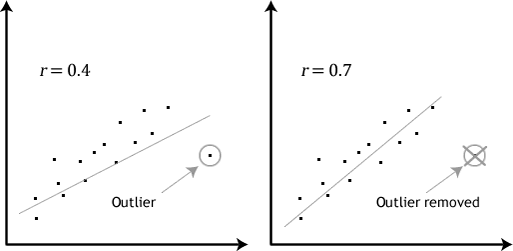
\includegraphics[width=3in]{figures/outliers-fig-1.png}

\caption{Deteccion de anomalias en un problema de regresión}
\label{fig:anomalias}
\end{figure}

En la figura ~\ref{fig:anomalias}  podemos ver como un dato anómalo puede perjudicar muy seriamente un problema de regresión lineal, el peso de la anomalía cambia completamente el comportamiento de nuestro modelo, ciertos algoritmos son mas sensibles a los outliers que otros, es un dato a tener en cuenta para saber la importancia que debemos darle a la detección de anomalías en nuestro proceso.

\subsubsection{Valores Faltantes}

En muchos casos, por no decir en una amplia mayoría van a existir datos con valores faltantes para ciertos atributos. Esto puede deberse a que para ciertos datos algunos atributos no tienen sentido o bien a la forma en que los datos fueron recolectados. Por ejemplo en un censo de la población todos los datos correspondientes al trabajo de una persona no se completan si la persona no tiene trabajo o bien si no quiere informarnos sobre su trabajo. 

El problema surge cuando los datos faltantes no son válidos para el algoritmo con el cual vamos a procesar la información. Algunos algoritmos admiten datos incompletos y otros no. En los casos en los que los datos incompletos no son admisibles debemos solucionarlos de alguna forma.

Una opción es eliminar aquellas observaciones para los cuales algún atributo tiene valores faltantes, esto es válido siempre y cuando sean solamente una pequeña minoría dentro de nuestro conjunto de datos. Cuando esto no es posible es necesario de alguna forma completar los atributos faltantes, a esto lo llamamos \textit{imputación}. 

El proceso de imputación de valores faltantes puede hacerse de muchas formas, una forma muy simple es completar con el valor promedio o la mediana para atributos numéricos y con el valor mas popular para atributos categóricos. Pero también podemos encarar el proceso de imputación como un mini-proceso interno de Data-Science, en cuyo caso completaríamos los atributos numéricos mediante un algoritmo de regresión y los datos categóricos con un algoritmo de clasificación. Lo que hacemos en estos casos es tomar todos los atributos que tiene nuestro dato y en base a estos atributos predecir los atributos faltantes tomando como set de entrenamiento el conjunto de datos para los cuales el atributo tiene algún valor. 

Existen varios algoritmos de imputación y algunos lenguajes cuentan con funciones para completar los valores faltantes en los datos automáticamente.

\subsection{Explorar los datos}

En este punto surge lo que llamamos "análisis de datos exploratorio" cuya principal característica es obtener un entendimiento básico de los datos con los cuales se va a trabajar sin tener ningún objetivo en particular. Es decir que simplemente exploramos los datos pero no pretendemos obtener respuestas a partir de los mismos. 
A continuación explicamos brevemente algunas tareas típicas del análisis exploratorio de datos

\subsubsection{Analizar la estructura de los datos} 
Analizamos la estructura general de los datos para entender con que información vamos a trabajar.
\begin{enumerate}
\item Ver cuantos datos (observaciones) tenemos en total
\item Ver cuantos atributos tiene cada observación
\item Ver el nombre y tipo de dato de cada observación
\item Ver cuantos valores faltantes existen y en que proporción se presentan para cada atributo
\end{enumerate}

\subsubsection{Navegar los datos} 

Una vez que conocemos los atributos y sus tipos de datos podemos visualizar los datos como si fueran una planilla de cálculo o simplemente como texto. Esta navegación muy básica nos permite entender cuáles son los valores de nuestros atributos, cuáles son los valores mas populares, en qué casos hay valores faltantes y detectar algunas posibles anomalías 

\subsubsection{Resumen estadístico}

Una herramienta fundamental del análisis exploratorio es hacer un resumen estadístico de cada atributo de nuestros datos, algunos datos importantes a conocer son:
\begin{enumerate}
\item Valor máximo y mínimo
\item Promedio y media
\item Cantidad de valores faltantes y proporción
\item Quantiles
\item Desviación standard
\end{enumerate}

\subsubsection{Visualizar los datos}

Esta es una etapa fundamental, la idea es simplemente visualizar gráficamente diferentes aspectos de nuestros datos, podemos realizar todo tipo de ploteos exploratorios, como por ejemplo de un atributo contra otro, o de un atributo solo a lo largo de todo el conjunto de datos. Este análisis es muy útil para determinar varias cosas: en primer lugar podemos ver el grado de correlación entre los atributos, algunos atributos están muy relacionados entre sí mientras que otros son independientes. Podemos también observar posibles anomalías en los datos cuando algunas de nuestras observaciones tengan valores que sobresalen del resto. Finalmente podemos apreciar o inferir el valor predictivo de ciertos atributos. 
Para ilustrar la importancia del análisis exploratorio vamos a mostrar un caso famoso que se conoce como "el cuarteto de Anscombe" la tabla 1.5 nos muestra los datos en forma tabular.

\begin{table}[!hbt]
\center{
\begin{tabular}{|c|c|c|c|c|c|c|c|}\hline
X1 & Y1 & X2 & Y2 & X3 & Y3 & X4 & Y4\\ \hline\hline
10 & 8.04  & 10 & 9.14 & 10 & 7.46 & 8  & 5.58\\
8 & 6.95 & 8 & 8.14 & 8 & 6.77 & 8 & 5.76 \\
13 & 7.58 & 13 & 8.74 & 13 & 12.74 & 8 & 7.71\\
9 & 8.81 & 9 & 8.77 & 9 & 7.11 & 8 & 8.84\\
11 & 8.33 & 11 & 9.26 & 11 & 7.81 & 8 & 8.47 \\
14 & 9.96 & 14 & 8.1 & 14 & 8.84 & 8 & 7.04\\
6 & 7.24 & 6 & 6.13 & 6 & 6.08 & 8 &5.25\\
4 & 4.26 & 4 & 4.1 & 4 & 5.39 & 19 & 12.5\\
12 & 10.84 & 12 & 9.13 & 12 & 8.15 & 8 & 5.56\\
7 & 4.82 & 6 & 7.26 & 7 & 6.42 & 8 & 7.91\\
5 & 5.68 & 5 & 4.74 & 5 & 5.73 & 8 & 6.89\\ \hline
\end{tabular}
}
\vskip 0.25cm
\caption{El cuarteto de Anscombe en versión tabular.}
\end{table}

Tenemos cuatro tablas con dos atributos cada una: $X$ e $Y$. Si calculamos algunas estadísticas de nuestros datos obtenemos la información de la tabla 1.6.

\begin{table}[!hbt]
\center{
\begin{tabular}{|c|c|c|c|}\hline
VAR & SUM & AVG & STD \\ \hline\hline
X1 & 99 & 9 & 3.32 \\
Y1 & 82.51 & 7.5 & 2.03 \\
X2 & 99 & 9 & 3.32 \\
Y2 & 82.51 & 7.5 & 2.03 \\
X3 & 99 & 9 & 3.32\\
Y3 & 82.50 & 7.5 & 2.03 \\
X4 & 99 & 9 & 3.32 \\
Y4 & 82.51 & 7.5 & 2.03 \\ \hline
\end{tabular}
}
\vskip 0.25cm
\caption{Estadísticas sobre el cuarteto de Anscombe.}
\end{table}

Como podemos ver todos los valores de X e Y presentan el mismo promedio, suma de valores y desviación standard, es decir que podríamos decir que estadísticamente X1-Y1, X2-Y3, X3-Y3 y X4-Y4 son iguales. Sin embargo si graficamos estos cuatro plots vemos lo siguiente:

\begin{figure}[!htb]
\centering
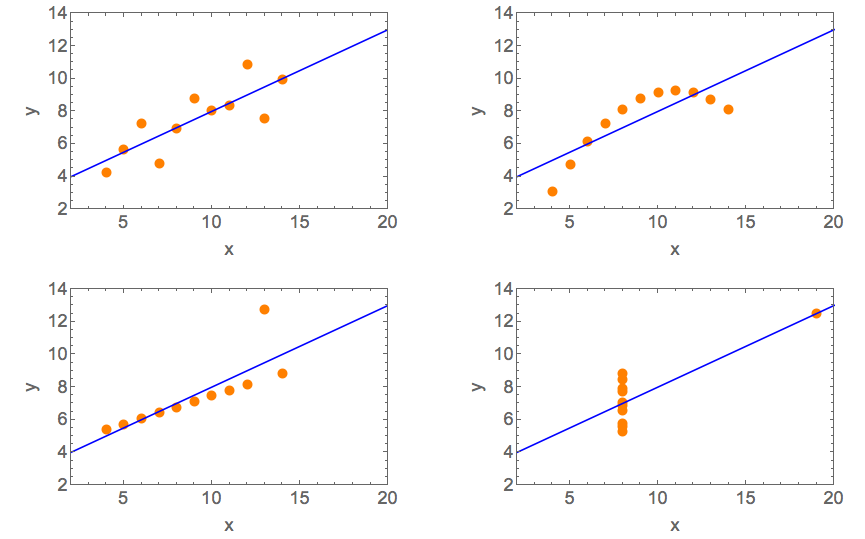
\includegraphics[width=3.2in]{figures/ascombe-fig-2.png}
\caption{Visualización del cuarteto de Anscombe}

\end{figure}

Como podemos ver datos que son estadísticamente idénticos pueden ser completamente diferentes graficamente, por eso es sumamente importante realizar todo tipo de plots para tener un buen conocimiento del conjunto de datos con el que trabajamos. El cerebro humano procesa la información gráfica de forma mucho mas eficiente que los números, podemos entender facilmente la "forma" de los datos del cuarteto de Anscombe al ver los plots pero esta forma no es tan fácil de visualizar si solamente vemos la tabla con los datos en forma numérica. 
Estos plots no tienen que ser ni lindos ni tampoco detallados son simplemente herramientas para rápidamente dar un vistazo gráfico a los datos. 

Uno de los plots mas usados para el análisis exploratorio es el que nos muestra la correlación que existe entre las variables de nuestro set de datos.Veamos un ejemplo de este plot para el set de datos "Iris".

Iris es un set de datos sobre flores en el que hay cuatro variables y una clase. Las variables son el ancho y alto de los pétalos y el ancho y alto de los sépalos. El objetivo de este set de datos es ver si con esta información es posible determinar a que especie pertenece la flor, las especies son en total 4. Para hacer el plot de correlación usamos únicamente los atributos, es decir que quitamos de nuestro set de datos el atributo que indica la especie a la cual pertenece la flor.

\begin{figure}[!htb]
\centering
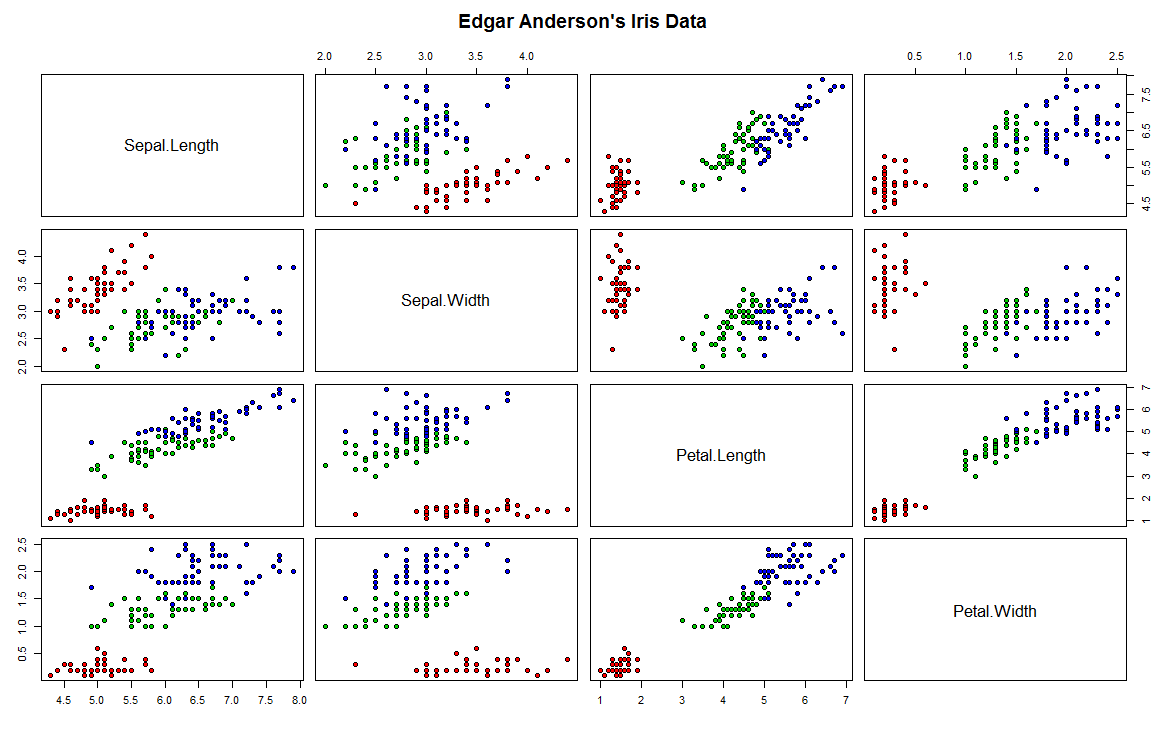
\includegraphics[width=5in]{figures/iris-fig-1.png}
\caption{Plot de correlación Para Iris}
\label{fig8}

\end{figure}

Entender este plot es muy simple, tenemos cuatro filas y cuatro columnas correspondientes a los cuatro atributos de nuestro set de datos, cada "celda" $M_{ij}$ de nuestra matriz representa el plot del atributo $i$ contra el atributo $j$,la diagonal tiene simplemente el nombre del atributo ya que no tiene sentido plotear un atributo contra si mismo. 

Para "Iris" podemos ver que existe una correlación lineal bastante fuerte entre el atributo "3" y el "4" es decir el largo y alto de los pétalos de las flores. También parece existir una correlación entre el largo de los sépalos (atributo 1) y el largo de los pétalos (atributo 3). Esto nos permitiría suponer que podemos usar tres o incluso dos de los atributos que tenemos para predecir la especie a la cual pertenece la flor es decir que nuestro set de datos que originalmente está en cuatro dimensiones podría funcionar en tres o dos dimensiones. Estas observaciones sobre la dimensionalidad de los datos serán muy importantes mas adelante.

\subsection{Aplicar a los datos el algoritmo necesario}

Una vez que los datos han sido depurados estamos en condiciones de aplicar el o los algoritmos necesarios para responder las preguntas que tenemos. Esta es la fase mas interesante de todo el proceso, donde realmente ocurre la magia, no vamos a hablar en detalle sobre los algoritmos que podemos aplicar ya que todo el resto del curso trata sobre este tema.

\subsection{Comunicar los resultados}

La última etapa del proceso es comunicar los resultados logrados, las respuestas a las preguntas que nos hicimos en un principio. En general esto implica la creación de reportes o visualizaciones que nos permitan transmitir las conclusiones a las que hemos llegado a partir de los datos. Como hemos mencionado previamente las personas entienden los gráficos de una forma mucho mas eficiente que una tabla de números o una narrativa, es por esto que la comunicación de resultados esta dominada por visualizaciones. Vamos a dedicar un extenso capítulo a la visualización de datos mas adelante.

\section{Formatos de Datos}

En esta sección vamos a comentar y analizar brevemente formatos de datos que son populares en Data Science, estos formatos extienden en cierta forma las estructuras de datos tradicionales como vectores, matrices y listas.

\subsection{Data Frames}

El \textit{Data Frame} es la estructura de datos más común e importante en un proceso de Data Science, es equivalente a una tabla en donde tenemos cada dato/observación como una fila y cada atributo como una columna.Cada columna tiene un tipo de dato, no es válido tener en una misma columna datos de diferente tipo. 

\begin{figure}[!htb]
\centering
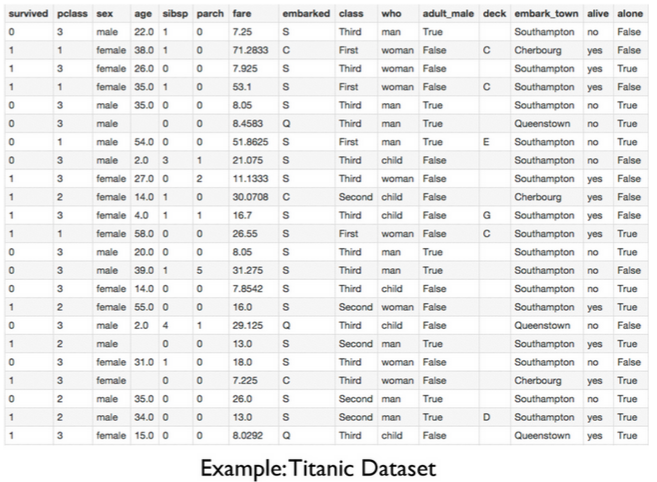
\includegraphics[width=5.2in]{figures/titanic-fig-1.png}
\caption{Titanic Dataset}

\end{figure}

Hay dos forma de ver a un data-frame: como un conjunto de filas o como un conjunto de columnas.Si pensamos en un data-frame como un conjunto de columnas entonces el data-frame es una lista de vectores en donde cada vector representa a un atributo (columna). Desde el punto de vista de la semántica de las estructuras de datos vamos a considerar que todos los datos en un vector deben ser del mismo tipo mientras que los datos dentro de una lista pueden ser de diferente tipo. 
Si consideramos a un data-frame como un conjunto de filas entonces el data-frame es un vector de diccionarios en donde cada diccionario representa los datos de cada una de nuestras observaciones o datos. 

Cada columna de un dataset puede ser de los siguientes tipos de datos:
\begin{itemize}
\item Caracteres: Strings o texto que pueden tomar cualquier valor, por ejemplo el nombre de una persona.
\item Numericos: Enteros o flotantes (subtipos) por ejemplo la edad de una persona o el precio de un artículo
\item Factores: Datos categóricos para los cuales existe una lista de valores posibles, por ejemplo Si/No 
\item Fechas: Datos en formato de fecha o timestamp, pueden incluir Año, Mes, Dia, Hora, Minutos y Segundos.
\end{itemize}

En el set de datos "Titanic" tenemos columnas de diferentes tipos. "Class" es un factor que puede ser "First","Second","Third" o "Crew" indicando a que clase pertenecía el pasajero. "Sex" es un factor que indica el género del pasajero y puede ser "Male" o "Female".  "Age" es una columna numérica que indica la edad del pasajero. "Survived" es un factor que indica si el pasajero sobrevivió a la tragedia.

Desde el punto de vista de las estructuras de datos el único tipo especial son los factores. Para representar un factor necesitamos un vector de valores posibles y luego podemos codificar el valor que cada dato toma para dicho factor mediante un índice al vector de valores posibles. De esta forma si el atributo "sex" de una persona puede ser "Male" o "Female" podemos representar con 1 el valor "Male" y con 2 el valor "Female" (o con 0 y 1 según convención). 

Los tipos de datos mas comunes en un data frame son entonces:

\begin{enumerate}
\item Numéricos y continuos
\item Numéricos y discretos
\item Texto
\item Fechas
\item Categóricos o Factores (n valores posibles) no-ordinales (el orden no importa ejemplo: red, blue, green)
\item Categóricos o Factores (n valores posibles) ordinales (el orden importa ejemplo: low, medium, high)
\end{enumerate}


\subsubsection{Codificación de Atributos Categóricos}

Consideremos el caso de atributos categóricos es decir en el cual tenemos una lista de valores posibles. Algunos ejemplos son atributos de tipo Si/No, provincia, sexo, color de un objeto, la clase a la cual pertenecía un pasajero del Titanic, etc. En todos los casos cada observación toma para el atributo en cuestión un valor que pertenece a una lista de valores posibles.

En muchos casos a un algoritmo le resulta confuso entender los datos de tipo categóricos por lo que es conveniente transformarlos en un formato equivalente pero mas simple de procesar para el algoritmo. Vamos a ver tres posibles ejemplos de codificación para los siguientes datos:

\begin{table}[!hbt]
\center{
\begin{tabular}{|c|c|}\hline
Pasajero & Clase \\ \hline
John Smith & First Class\\
Susan Walters & Third Class\\
Megan Smith & First Class\\
Willie Wilburg & Second Class\\ \hline
\end{tabular}
}
\vskip 0.25cm
\caption{Codificación de atributos categóricos.}
\end{table}

Nuestro atributo categórico puede tomar 3 valores: "First Class", "Second Class" y "Third Class". 

Una primera aproximación es simplemente reemplazar el atributo por un número que indica a cual de los $n$ valores corresponde el mismo.A esto lo llamamos \textbf{codificación ordinal}

\begin{table}[!hbt]
\center{
\begin{tabular}{|c|c|}\hline
Pasajero & Clase \\ \hline
John Smith & 1\\
Susan Walters & 3\\
Megan Smith & 1\\
Willie Wilburg & 2\\ \hline
\end{tabular}
}
\vskip 0.25cm
\caption{Codificación Ordinal.}
\end{table}

La codificación ordinal no suele tener muy buenos resultados, al codificar valores categóricos como numéricos introducimos en nuestros datos propiedades que no son ciertas. Por ejemplo si codificamos 1=azul, 2=verde, 3=rojo un algoritmo puede deducir que 2*azul = verde o que azul+verde = rojo y esas relaciones no son ciertas.

La siguiente codificación se denomina \textbf{"one hot encoding"} y consiste en dividir el atributo en tantas columnas como valores posibles puede tener y usar cada columna como un dato binario indicando si el atributo toma o no dicho valor.

\begin{table}[!hbt]
\center{
\begin{tabular}{|c|c|c|c|}\hline
Pasajero & First Class & Second Class & Third Class \\ \hline
John Smith & 1 &0 &0\\
Susan Walters & 0&0&1\\
Megan Smith & 1&0&0\\
Willie Wilburg & 0&1&0\\ \hline
\end{tabular}
}
\vskip 0.25cm
\caption{One Hot Encoding.}
\end{table}

One-hot encoding es una codificación muy popular pero lamentablemente no escala muy bien. En primer lugar es necesario construir en memoria un diccionario por cada feature en donde asociaremos un número a cada posible valor de cada columna, este diccionario puede ser demasiado grande. Otro problema serio es que si una columna puede tomar muchos valores diferentes posibles, por ejemplo una URL, entonces podemos necesitar miles o millones de nuevas columnas para representar los datos, en muchos problemas concretos esto no es viable.

One-hot encoding es un método simple pero frecuentemente no es viable.

Una tercera variante consiste en convertir los datos a un número como hicimos en la codificación ordinal y luego representar dicho número como un binario de $\log(k)$ bits siendo $k$ la cantidad de valores que puede tomar el atributo. Luego representamos cada bit como una columna binaria.

\begin{table}[!hbt]
\center{
\begin{tabular}{|c|c|c|}\hline
Pasajero & bit1& bit0 \\ \hline
John Smith & 0 &1\\
Susan Walters & 1&1\\
Megan Smith & 0&1\\
Willie Wilburg & 1&0\\ \hline
\end{tabular}
}
\vskip 0.25cm
\caption{Codificación binaria.}
\end{table}

La \textbf{codificación binaria} es un compromiso entre one-hot encoding y la codificación ordinal. Funciona mejor que la codificación ordinal pero requiere menos columnas que one-hot enconding. Notar que usamos 01,10 y 11 para las clases pero podríamos haber usado 00,01 y 10 respectivamente. 

Nuestro siguiente esquema de codificación se denomina \textbf{Feature Hashing} o \textbf{The hashing trick} y está basado en el uso de una función de hashing para determinar el número de columna de cada dato. 
Usando feature-hashing podemos definir la cantidad de columnas que queremos usar: $m$ y luego simplemente aplicar a cada valor de las variables categóricas una función de hashing que devuelva un número entre $0$ y $m-1$ incrementando dicha posición. Notemos que usando este esquema podemos mezclar muchas columnas categóricas en un mismo espacio de features de dimensión $m$ y que no es necesario conocer cuáles pueden ser todos los valores posibles, tampoco es importante la cantidad de valores diferentes que puede tomar cada variable categórica.

Feature-hashing es un método extremadamente eficiente y terriblemente popular, para que funcione muy bien es conveniente minimizar las colisiones lo cual se logra usando un número $m$ grande, frecuentemente $m$ puede estar en el orden de los miles o incluso millones de dimensiones. En algunos casos esta cantidad de dimensiones es muy grande y el método se vuelve poco-práctico.

Vamos a desarrollar feature-hashing con mayor detalle y estudiar sus fundamentos teóricos mas adelante.

\subsubsection{Codificación de atributos categóricos en gran escala}

Abordamos ahora el caso extremo de codificación de atributos categóricos, tenemos millones o billones de datos en donde los atributos categóricos pueden tener millones de valores posibles. Este caso es muy frecuente en problemas de análisis de datos y machine learning por lo que debemos dedicarle un cierto tiempo.

A modo de ejemplo consideremos el caso en el cuál queremos predecir si un usuario va a hacer click o no en un aviso de una página web. Nuestro set de datos puede tener el siguiente formato:

\begin{table}[!hbt]
\center{
\begin{tabular}{|c|c|c|c|c|}\hline
UserId & URL & AdId & Referer & Click \\ \hline
10983 & http://... & 89318 & http://.... & 1 \\ \hline
\end{tabular}
}
\vskip 0.25cm
\caption{Atributos categóricos en gran escala.}
\end{table}

Aquí tanto el UserId como el AddId, la URL o el referer son variables categóricas que pueden tomar millones de valores posibles. Si queremos usar un algoritmo de MachineLearning para predecir la variable click tendremos como problema la codificación de las variables categóricas, si agregamos que la cantidad de datos es enorme el problema se convierte en un caso difícil.

Una solución sumamente elegante a este problema es reemplazar cada variable categórica por un conjunto muy limitado de contadores. Por ejemplo podemos reemplazar cada variable categórica por dos contadores: $N+$ y $N-$ que indican la cantidad de veces que dicho valor aparece en las filas para las cuales clicks=1 y clicks=0 respectivamente. Por ejemplo si tenemos AdId=8907 y sabemos que el aviso 8907 fue clickeado 20 veces y fue ignorado 1097 veces entonces reemplazamos la columna AdId por los valores 20 y 1097.

\begin{table}[!hbt]
\center{
\begin{tabular}{|c|c|c|c|c|c|}\hline
UserId & URL & AdId N+ & AdId N- & Referer & Click \\ \hline
10983 & http://... & 20 & 1097 & http://.... & 1 \\ \hline
\end{tabular}
}
\vskip 0.25cm
\caption{Count encoding.}
\end{table}

A este método lo denominamos \textbf{count-encoding} y lo podemos aplicar a todas las columnas de nuestro set de datos. Podemos agregar también una columna que exprese el logarimo de la relación entre N+ y N-, por ejemplo $\log(N+ - N-)$, de esta forma cada columna categórica de nuestro Datset queda representada  como una cantidad muy pequeña de nuevas columnas y la cantidad de columnas a crear no depende de la cantida de valores posibles del atributo categórico.

Para aplicar count-encoding hay que tener cuidado con una cuestión muy importante: si usamos el set de entrenamiento para obtener los contadores y luego codificamos el mismo set hay una enorme posibilidad de que el algoritmo sea capaz de deducir el label de un dato en función de los contadores lo cual es muy perjudicial para construir algoritmos predictores.

Hay dos posibles soluciones a este problema: una es separar el set de entrenamiento en dos partes (split count-encoding) usando la primera parte para obtener los contadores por cada feature y la segunda parte para codificar y entrenar al algoritmo. Este método tiene como ventaja que es muy simple pero desperdicia gran parte del set de entrenamiento, si tenemos billones de datos para entrenar es perfectamente viable.

Si la cantidad de datos hace que el método anterior no sea viable entonces podemos solucionar el problema agregando algo de ruido a los contadores, el método mas usado está basado en principios de privacidad diferencial y consiste en agregar ruido a partir de la distribución de Laplace. L(0,3) es suficiente en la mayoría de los casos. Este ruido hace que cada dato se "mezcle" un poco con sus vecinos y por lo tanto no es posible determinar el label a partir de los contadores ya que hay varios casos posibles. 

\begin{table}[!hbt]
\center{
\begin{tabular}{|c|c|c|c|}\hline
atributos & Datos & Algoritmo &Codificación \\ \hline
Pocos, decenas & - & - & One-hot encoding \\
cientos o miles & - & - & Binary encoding \\
Miles o millones & - & Lineales & Feature-Hashing \\
Miles o millones & millones & No-lineales & split Count-encoding o Laplace Count-encoding\\
Miles o millones & no tantos & No-lineales & Laplace Count-encoding \\ \hline
\end{tabular}
}
\vskip 0.25cm
\caption{Codificación de atributos categóricos.}
\end{table}

Finalmente queremos destacar que el proceso de obtener los contadores puede realizarse de forma muy eficiente usando el algoritmo Count-Min que vamos a ver en el capítulo sobre algoritmos de streaming.

La tabla nos puede ayudar a terminar de entender el tema de codificiación de atributos categóricos:

\subsection{Texto}

Los textos en formato plano son uno de los formatos mas simples y habituales en un proceso de Data-Science, a partir de un conjunto de textos podemos extraer una gran cantidad de información, por ejemplo podemos realizar consultas, buscar frases o palabras, hacer un resumen automático de textos, analizar las palabras (keywords) o frases mas relevantes, responder preguntas en lenguaje natural,  etc.
Todas los procesos que involucran texto necesitan que de alguna forma transformemos los textos en un conjunto de datos que nuestros algoritmos puedan procesar, en esta sección introducimos el modelo mas simple para modelar textos denominado "bag of words" (BOW). Mas adelante veremos modelos mucho mas sofisticados.

\subsubsection{Bag of Words (BOW)} En el modelo BOW cada texto se representa con un vector de "n" dimensiones siendo "n" la cantidad total de términos (palabras) en la colección. De esta forma si hay 300.000 palabras en total cada texto está representado por un vector de 300.000 dimensiones. El vector contiene simplemente la cantidad de veces que cada palabra aparece en el texto. 

Consideremos el siguiente ejemplo:

\begin{quotation}
Once there was a king\\
the king was good\\
\end{quotation}

Suponiendo que no hay mas texto que lo que vemos tenemos un vocabulario (léxico) de 7 palabras:

\begin{enumerate}
\item once
\item there
\item was
\item a
\item king
\item the
\item good
\end{enumerate}

Es decir que podemos representar a nuestros textos con vectores de 7 elementos. Si consideramos a cada línea de nuestro texto como un documento independiente entonces tendríamos dos vectores:

\begin{verbatim}
(1,1,1,1,1,0,0)
(0,0,1,0,1,1,1)
\end{verbatim}

El primer elemento de cada vector corresponde a la primera palabra y así sucesivamente. En este ejemplo muy simple tenemos muy pocas palabras y muy pocos documentos en general para un conjunto de documentos grandes los vectores pueden llegar a tener cientos de miles de dimensiones y son vectores muy dispersos ya que la mayoría de sus elementos son ceros. Esto se debe a que es mucho mas probable que un documento no tenga una palabra cualquiera a que la tenga. 

\subsection{Datos Matriciales}

Una matriz es una simplificación de un data-frame, la matriz es un conjunto de valores numéricos formateados en "m" filas y "n" columnas. Es interesante destacar que un gran número de problemas de Data-Science se presentan en forma de matrices.
Es de destacar que excepto los strings todos los tipos de datos que hemos visto se pueden asociar a un valor numérico, los factores se pueden codificar con one-hot encoding o alguna otra de las codificaciones vistas, las fecha pueden convertirse en un offset en segundos a partir de un cierto EPOCH y los valores numéricos no hace falta convertirlos. Es por esto que en la mayoría de los casos podemos convertir el set de datos en una matriz numérica con la cual trabajar.

\subsubsection{Matrices Dispersas} En muchos casos las matrices con las cuales trabajamos son dispersas es decir que tienen una gran mayoría de ceros y muy pocos elementos distintos de cero. En estos casos es necesario contar con formatos especiales que nos permitan almacenar la matriz de forma eficiente. En modo texto un formato de archivo que es eficiente para almacenar matrices dispersas es el formato de LIBSVM en el cual cada línea del texto representa a una fila de la matriz, el formato de LIBSVM establece que el primer elemento de cada línea es el "label" correspondiente a la fila y luego se indican los elementos distintos de cero con la notación $col:value$ es decir número de columna y valor. 

Por ejemplo si tenemos el siguiente archivo LIBSVM:

\begin{verbatim}
label1 2:4 5:3
label2 1:3 
label3 2:2
\end{verbatim}

La matriz representada es la siguiente:

$$
\begin{pmatrix} 
0 & 4 & 0 & 0 & 3 \\
3 & 0 & 0 & 0 & 0 \\
0 & 2 & 0 & 0 & 0 \\
\end{pmatrix}
$$

El formato es sencillo de entender. En memoria hay varias formas de trabajar con matrices dispersas, un mecanismo que suele funcionar bien y es muy usado es el llamado "compressed row storage" (CRS).

\subsubsection{CRS (Compressed Row Storage)} Usando CRS una matriz dispersa se almacena mediante tres vectores. El primer vector ($V1$) almacena los elementos distintos de cero de la matriz. El segundo vector ($V2$) almacena los números de columna en los que aparecen los elementos distintos de cero de la matriz. El tercer vector ($V3$) indica el índice al primer vector para los elementos que son el inicio de una nueva fila en la matriz. 

Para la matriz de nuestro ejemplo los vectores serían los siguientes:

\begin{verbatim}
V1 = (4,3,3,2)
V2 = (2,5,1,2)
V3 = (1,3,4)
\end{verbatim}

Notar que en todos los casos usamos como convención numerar filas y columnas a partir de 1, indistintamente puede numerarse a partir de cero.

Los vectores $V1$ y $V2$ tienen igual cantidad de elementos: tantos como elementos distintos de cero haya en la matriz original. El vector $V3$ tiene tantos elementos como filas tenga la matriz. 
Usando CRS es posible recuperar cualquier fila de la matriz sin necesidad de recorrerla completamente. Por ejemplo si queremos la fila 2 de la matriz sabemos que el segundo elemento de $V3$ nos apunta al primer elemento distinto de cero de la fila 2, es decir que el primer elemento distinto de cero es el tercer elemento de $V1$ y $V2$ es decir un 3 en la columna 1. Sabemos que la fila 2 solo tiene un elemento distinto de cero ya que el siguiente elemento de $V3$ es el índice 4 y corresponde a la fila 3, por lo tanto la fila 2 de la matriz es:

\begin{verbatim}
(3,0,0,0,0,0)
\end{verbatim}

\subsection{Imágenes}

Las imágenes también suelen ser un set de datos habitual en problemas de Data Science, una imagen se representa en general mediante un tensor de $X*Y*3$ elementos. Siendo $X$ e $Y$ el largo y alto de la imagen en pixeles. El "3" se debe a que por cada pixel almacenamos tres valores correspondientes a los canales RGB, de esta forma cada pixel de la imagen queda representado por el valor de intensidad del mismo para el canal rojo, verde y azul que en general se representa mediante un número de 8 bits lo cual nos da una profundidad de color de 24 bits.


\section{Niveles de Almacenamiento}

En todo proceso de análisis y procesamiento de datos podemos distinguir tres niveles de almacenamiento, tres diferentes lugares en donde pueden estar alojados los datos que tenemos que procesar.
\begin{enumerate}
\item En Memoria
\item En Disco
\item En un Cluster
\end{enumerate}

\subsection{Datos en Memoria}
La memoria es el medio mas eficiente en cuanto a velocidad para almacenar los datos pero también es el mas costoso, aún asi hoy en día muchos, tal vez la mayoría de los sets de datos, pueden ser alojados en memoria para ser procesados de forma eficiente.

Cuando los datos están alojados en memoria podemos organizarlos usando diferentes estructuras de forma tal de poder acceder a un dato buscado sin necesidad de recorrer todos los datos. Incluso en memoria recorrer todos los datos puede ser un proceso costoso. Algunas de las estructuras de datos mas populares para almacenar datos en memoria son:

\begin{enumerate}
\item Tablas de hash (diccionarios)
\item Arboles binarios y variantes
\item Tries y variantes
\item Listas
\item Indices Invertidos
\item Skip-Lists
\end{enumerate}

En general es conveniente tener un manejo adecuado de estas estructuras de datos para poder operar eficientemente con datos a nivel de memoria. En concreto los diccionarios y las tablas de hash son estructuras que vamos a usar muy frecuentemente. Algunos de estos temas los vamos a desarrollar en los siguientes capítulos.

\subsection{Datos en Disco}

Los datos se almacenan en disco como forma de soporte permanente ya que la memoria es volátil, la forma de almacenar los datos en disco puede ser mediante archivos o bien una base de datos. Existen diversos tipos de archivos y bases de datos para persistir datos en disco, las bases relacionales son las mas populares y durante muchos años fueron la herramienta ubicua para almacenar y procesar datos. Luego aparecieron las bases No-SQL que son bases de datos especializadas en cierto tipo de información como por ejemplo documentos de texto o grafos. Mas adelante dedicaremos algo de tiempo a ver este tipo de bases de datos.

En una gran cantidad de problemas las bases de datos no son necesarias y se usan simples archivos para almacenar los datos, estos archivos pueden ser de tipo .CSV, .TXT, JSON u otros formatos. Los formatos basados en XML que fueron muy populares, hoy en día han caído en desuso ya que agregan la complejidad del proceso de XML a la complejidad propia de los datos.

En general no es una buena idea operar sobre datos almacenados en disco ya que las velocidades de acceso y transferencia de los mismos son bastante lentas. El modelo mas usado consiste en levantar los datos a procesar en memoria y realizar los procesos necesarios repitiendo este proceso tantas veces como sea necesario. En los contados casos en los cuales es necesario procesar los datos sobre el disco mismo es conveniente recordar que la forma mas eficiente de procesar datos en disco es accediendo a los mismos de forma secuencial. Dos o incluso tres lecturas secuenciales suelen ser mas eficientes que leer de forma aleatoria es decir accediendo a los datos mediante referencias a los mismos. Esto es entendible debido a que en una lectura secuencial no hace falta realizar "seeks" que es una operación costosa en un disco. En los dispositivos SSD que no tienen necesidad de hacer "seek" leer secuencialmente o de forma aleatoria es mas o menos equivalente.

\subsection{Datos en un Cluster}

Cuando los datos son tan masivos para exceder la capacidad de almacenamiento de uno o varios discos no queda mas remedio que almacenarlos en un cluster, es decir distribuidos en varios equipos. Los volúmenes de información que se manejan actualmente hacen que esta forma de almacenamiento y procesamiento de datos sea cada vez mas popular y necesaria por lo que dedicaremos el próximo capítulo a los pormenores y detalles del almacenamiento y procesamiento distribuido.

\section{La Ley de Zipf y las Leyes de Potencias}

La ley de Zipf describe datos en los cuales hay muy pocos eventos de mucha magnitud (impacto) y muchos eventos de muy baja magnitud. El ejemplo mas tradicional es la frecuencia de las palabras de un determinado idioma en un texto o conjunto de textos. Algunas palabras, que son muy pocas, como "the" aparecen una enorme cantidad de veces mientras que hay una enorme cantidad de palabras con frecuencia muy baja. Otro ejemplo es la cantidad de visitas a sitios web. Algunos pocos sitios web tienen muchísimos visitantes mientras que existen millones de sitios con muy pocas visitas. 

\begin{figure}[!htb]
\centering
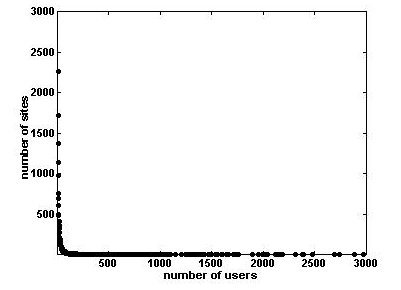
\includegraphics[width=3in]{figures/zipf1.png}

\caption{Cantidad de visitas a sitios web}
\label{fig:zipf1}
\end{figure}

La figura ~\ref{fig:zipf1} nos muestra el gráfico de visitas para usuarios de AOL en un cierto período de tiempo. El gráfico tiene una forma de "L" casi perfecta, hay muchos sitios con muy pocas visitas (users) y muy pocos sitios con muchísima cantidad de visitas. 

Este gráfico es muy difícil de interpretar, la verdadera aparición de la ley de Zipf y las leyes de potencias se evidencia si graficamos usando en los ejes escalas logarítmicas.

\begin{figure}[!htb]
\centering
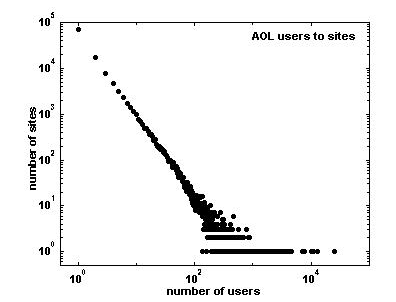
\includegraphics[width=3in]{figures/zipf2.png}

\caption{Cantidad de visitas a sitios web. Log-Log plot.}
\label{fig:zipf2}
\end{figure}

En la figura ~\ref{fig:zipf2} vemos el mismo plot en escala logarítmica como podemos ver el gráfico es ahora una recta, con algo de ruido en la parte final. Esta es la marca característica de lo que llamamos una \textit{ley de potencias} (power-law) y que, como vremos, es sinónimo de una distribución que obedece la ley de Zipf.

Cada vez que un plot en escala logarítmica presenta una recta existe la confusión de si estamos viendo una ley de potencias, la ley de zipf o la distribución de Pareto. En realidad son tres formas diferentes de interpretar el mismo tipo de distribución, a continuación explicamos cuáles son sus definiciones y equivalencias para dejar en claro estos conceptos que son muy importantes.

\subsection{Pareto, Zipf y Power-Laws}

La ley de Zipf fue enunciada por George Kingsley Zipf un linguista de Harvard que estaba interesado en determinar la frecuencia de la i-ésima palabra mas frecuente en un cierto idioma. Se define, entonces, en base al ranking de cada uno de los eventos ordenados por frecuencia y dice que la frecuencia de un evento es inversamente proporcional a su ranking. Esto quiere decir que si en un texto tenemos la palabra "the" que ocurre 4000 veces podemos esperar que la palabra siguiente en frecuencia ocurra 2000 veces la siguiente 4000/3 veces etc. En definitiva si llamamos $f$ a la frecuencia de un evento tenemos que la frecuencia puede calcularse como:

\begin{myequation}
f \approx r^{-b}
\end{myequation}

En donde el exponente $b$ es un valor muy cercano a 1. Esto quiere decir que si ploteamos en el eje X el ranking y en el eje Y la frecuencia y usamos una escala logarítmica obtenemos una recta cuya pendiente es muy similar a -1. 

Por lo tanto la \textit{ley de Zipf} y las distribuciones Zipfianas se caracterizan por estudiar frecuencia en función de ranking y por presentar una recta cuya pendiente es -1 en un gráfico de escala logarítmica.

Pareto estaba interesado en la distribución de los ingresos entre la población. En lugar de preguntarse cuál es el i-ésimo ingreso mas alto le interesaba saber cuántas personas tenían un ingreso mayor a un cierto valor $x$. La \textit{ley de Pareto} está definida entonces en función de una función de acumulación de la distribución (CDF) y dice que la cantidad de eventos cuya frecuencia es mayor a $x$ es una potencia inversa de $x$.

\begin{myequation}
P[X>x] \approx x^{-k}
\end{myequation}

Esta ley nos indica que hay muy pocos billonarios y que la enorme mayoría de la población tiene ingresos pequeños. 

Las \textit{leyes de potencias} (power laws) son la versión mas simple de estos tres puntos de vista y nos dicen simplemente cuál es la frecuencia de un evento cuyo valor es $x$. Por ejemplo cuántas personas tienen un cierto ingreso $x$ o cuántos websites tuvieron una cierta cantidad de visitas. Es simplemente la distribución de probabilidades (PDF) asociada a la ley de Pareto. 

\begin{myequation}
P[X=x] \approx x^{-k+1} = x^{-\alpha}
\end{myequation}

Es decir que $\alpha=k+1$ en donde $k$ es el exponente de la ley de Pareto. Esto establece que la ley de Pareto es una ley de potencias. A continuación vamos a mostrar que también hay una relación directa entre la ley de Zipf y la ley de Pareto. En una ley de potencias tenemos que $y=C x^{-\alpha}$ lo cual implica que $\log(y) = \log(C) -\alpha \log(x)$. Esto nos muestra que una ley de potencias con exponente $\alpha$ es una recta cuya pendiente es $-\alpha$ en escala logarítimica. Podríamos tentarnos y decir que la recta que mejor ajusta al plot de los datos en escala logarítmica es una buena forma de obtener el exponente $\alpha$ asociado a la ley de potencias pero esto no sería una buena idea. 

El problema es que la cola final de la distribución (ver ~\ref{fig:zipf2}) es ruidosa, esto es porque a medida que aumentamos la frecuencia cada vez hay menos eventos que tienen dicha frecuencia. En el caso de nuestro ejemplo hay muy pocos websites que tienen una gran cantidad de visitas. 

La forma de corregir esto es discretizar los datos en intervalos cada vez mas grandes, por ejemplo el segundo intervalo puede ser el doble del primero, el tercero 4 veces el primero, etc. Luego dividimos la cantidad de puntos que caen dentro del intervalo por el ancho del mismo para normalizar. Con este procedimiento la cantidad de puntos en cada intervalo se hace pareja. En nuestro ejemplo a medida que pedimos mayor cantidad de visitas (users) agrupamos a mayor cantidad de sitios. Si es necesario un ejemplo numérico podemos imaginar que el primer intervalo va de 0 a 1 visita el segundo de 2 a 4 visitas el tercero de 4 a 8 visitas, etc. Los intervalos son cada vez mas grandes por lo que la cantidad de sitios va a ser mas pareja en cada uno.

\begin{figure}[!htb]
\centering
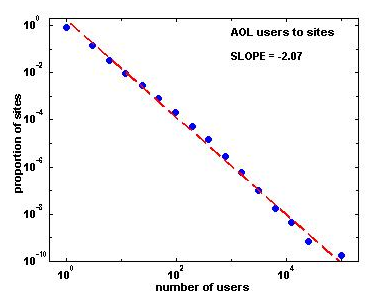
\includegraphics[width=3in]{figures/zipf3.png}

\caption{Cantidad de sitios por cantidad de visitas discretizada logarítimicamente en escala log-log normalizada}
\label{fig:zipf3}
\end{figure}

La figura ~\ref{fig:zipf3} nos muestra el resultado de hacer esto con los datos de las visitas a los websites. Podemos ver que hay mucho menos ruido. Si ajustamos ahora una recta al gráfico obtenemos una pendiente de -2.07. 

Otra forma de calcular el exponente de una ley de potencias es mediante la siguiente fórmula (derivada de la formulación de maximum likelihood para p(x))

\begin{myequation}
\hat{\alpha}=1+n(\sum\limits_{i=1}^{n} \ln \frac{x_i}{x_{min}})^{-1}
\end{myequation}

Una alternativa al procedimiento que hemos descripto es usar la distribución de Pareto $P[X>x]=x^{-k}$ el ruido de la cola se suaviza de forma natural en la acumulación de la distribución. 

\begin{figure}[!htb]
\centering
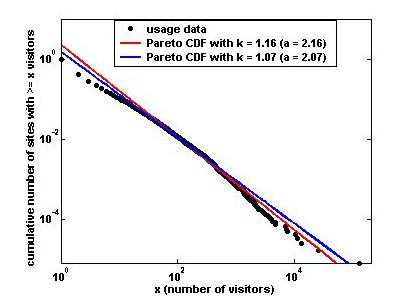
\includegraphics[width=3in]{figures/zipf4.png}

\caption{Distribución acumulada}
\label{fig:zipf4}
\end{figure}

En la figura ~\ref{fig:zipf4} vemos el gráfico en escala logarítmica de la cantidad de visitas en el eje x y el acumulado de número de sitios con al menos esa cantidad de visitas en el eje y (Pareto). Si ajustamos una recta a este gráfico obtenemos como pendiente $\alpha=-2.16$ que es un valor muy similar al que habíamos obtenido discretizando la ley de potencias. 

Grafiquemos ahora la cantidad de visitas en función del ranking del sitio (de 1 a N).

\begin{figure}[!htb]
\centering
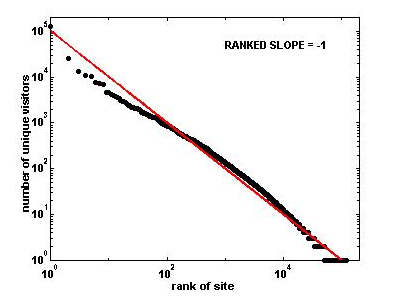
\includegraphics[width=3in]{figures/zipf5.png}

\caption{Ley de Zipf}
\label{fig:zipf5}
\end{figure}

Podemos observar en la figura ~\ref{fig:zipf5} que en escala logarítmica el plot tiene pendiente similar a -1 lo que nos indica que este set de datos cumple la ley de Zipf.

Podríamos pensar que tenemos dos leyes de potencias diferentes: una para la distribución de las frecuencias y otra para la ley de Zipf (ranking). La clave es formular el ranking de la forma adecuada para ver su relación con Pareto. La frase "El r-ésimo sitio mas visitado tiene n visitas" es equivalente a decir "r sitios tienen n o mas visitas" que es exactamente la definición de la distribución de Pareto pero con los ejes x e y intercambiados. Para Zipf tenemos a "r" (ranking) en el eje x y n (visitas) en el eje y mientras que para Pareto tenemos n (visitas) en el eje x y r en el eje y. Por lo tanto:

$$
n \approx r^{-b} \text{(Zipf)}
$$

Y entonces el exponente de Pareto es $1/b$ y vale:

$$
r \approx n^{-1/b} \text{(Pareto)}
$$

En esta última fórmula $n$ es cantidad de visitas y $r$ es cantidad de sitios que tienen $n$ o mas visitas.

Como hemos visto que la ley de potencias es una derivación directa de Pareto su exponente será $1+1/b$ lo cuál nos dice que Pareto, Zipf y la ley de Potencias son puntos de vista diferentes para el mismo fenómeno y la relación que existe para calcular uno en función de cualquiera de los otros.

\subsection{Leyes de Potencias}

El fenómeno que podemos interpretar como una ley de potencias, Zipf o Pareto se da en muchísimas situaciones en el mundo real. Algunas distribuciones de este tipo son:

\begin{figure}[!htb]
\centering
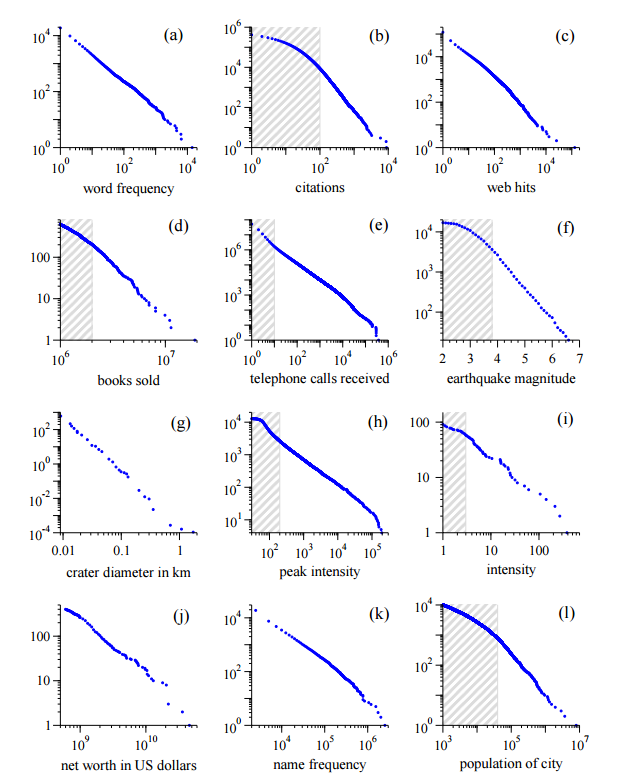
\includegraphics[width=4.3in]{figures/zipf6.png}

\caption{Plots de ranking/frecuencia para diferentes fenómenos. En escala logarítmica podemos ver que la pendiente de todos es muy similar a -1 lo cual evidencia que cumplen la ley de Zipf.}
\label{fig:zipf6}
\end{figure}

\begin{enumerate}
\item Frecuencia de las palabras en la mayoría de los lenguajes.
\item Cantidad de citas de papers científicos.
\item Cantidad de visitas a sitios web.
\item Cantidad de ventas de libros.
\item Cantidad de llamadas por línea telefónica.
\item Magnitud de terremotos.
\item Diámetro de cráteres lunares.
\item Intensidad de las tormentas solares.
\item Cantidad de amigos en una red social.
\item Frecuencias de nombres de personas.
\item Población de ciudades.
\item Ingreso neto de la población.
\end{enumerate}

\subsection{Propiedades de las Leyes de Potencias}

Un Power Law se caracteriza por una distribución de la forma:

\begin{myequation}
p(k_i=x) = x^{-\alpha}
\end{myequation}

\subsubsection{Necesidad de un valor mínimo}

La primera propiedad importante es que es necesario fijar un valor mínimo para $x$ ya que las leyes de potencias divergen si $x$ es un valor cercano a 0. Por ejemplo para las frecuencias de palabras funciona usar 1 como frecuencia mínima. Para la magnitud de los terremotos podríamos usar 3.8 en la escala de Richter, etc. 

\subsubsection{Diferencias con una exponencial}

En segundo lugar veamos en que se distingue una ley de potencias de una función de la familia exponencial:

\begin{figure}[!htb]
\centering
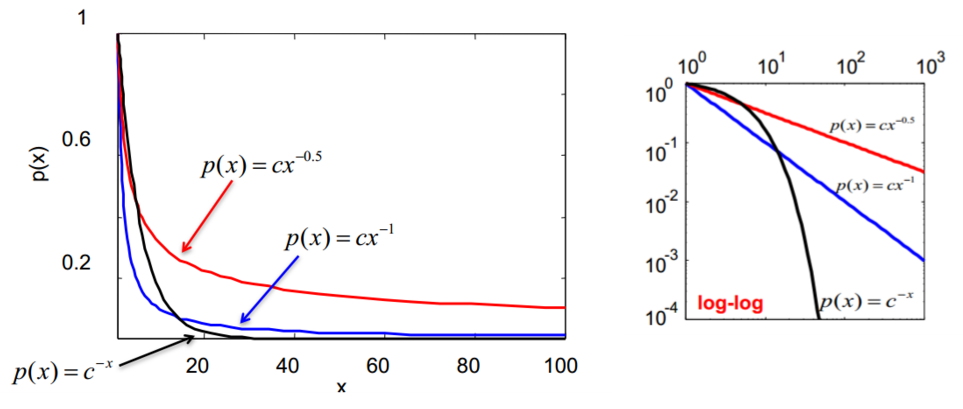
\includegraphics[width=4.3in]{figures/rs-fig-5.png}
\caption{Power Law vs Exponencial}

\end{figure}

La diferencia con una distribución exponencial es que el exponente es una constante. Al graficar la distribución del grado es difícil distinguirla de una exponencial, la diferencia matemática es que existe un valor $x$ a partir del cual la exponencial siempre es menor que una ley de potencias, esto es muy fácil de demostrar pero es muy difícil apreciarlo en un gráfico. La mejor forma de detectar una ley de potencias es hacer el gráfico con escala logarítmica, en cuyo caso la ley de potencias aparece como una recta mientras que una exponencial es una curva. 

\subsubsection{Dependencia de los eventos}

Podemos afirmar que los eventos que responden a una ley de potencias dependen entre sí. Si los eventos fueran independientes entonces su distribución acumulada sería normal de acuerdo al Teorema Central del límite. En el caso de las palabras la cantidad de veces que aparece una determinada palabra depende de las demás palabras. En otros casos esto es mas difícil de ver, en el caso de las llamadas telefónicas podemos afirmar que la cantidad de veces que se llama a un cierto número depende de los otros números, tal vez la forma correcta de explicar esto sea pensar que el que llama a muchos números tiene menos tiempo de llamar a otros.

\subsubsection{Invariancia a la escala}

Las leyes de potencias son invariantes a la escala. Si tenemos $y=x^{-\alpha}$ multiplicar a $x$ por una constante $c$ nos da: $cx^{-\alpha} = c^{-\alpha} x^{-\alpha} \approx x^{-\alpha}$

\subsubsection{Promedio y varianza}

Las leyes de potencias solo tienen promedio si el exponente $\alpha$ es mayor a 2 y tienen varianza infinita si el exponente es menor a 3. La mayoría de las leyes de potencias tienen $\alpha$ entre 2 y 3 por lo que tendrán promedio pero varianza infinita. La varianza infinita da origen al fenómeno del Cisne Negro (Black Swan). 

\subsubsection{Fenómeno del Cisne Negro}

El fenómeno del Cisne Negro ocurre cuando un evento es inesperado pero al mismo tiempo lógico. Si vemos un cisne blanco, luego otro cisne blanco, luego otro, y así durante miles de eventos cuando aparezca un cisne negro nos llevaremos una tremenda sorpresa. Sin embargo esto era lógico porque en la naturaleza hay tanto cisnes negros como blancos. 

\subsection{Origen de las leyes de potencias}

El motivo por el cual ciertos eventos responden a una ley de potencias no es claro, hay muchas teorías y estudios al respecto pero ninguno es conclusivo. En su tratado original Zipf justificó su ley basándose en el \textit{principio del mínimo esfuerzo}. Cuando dos personas se comunican usando un cierto lenguaje intentan usar la menor cantidad posible de palabras que transmitan la información que queremos comunicar. Si estudiamos la cantidad de información de cada palabra desde el punto de vista de la teoría de la información veremos que responde a la ley de Zipf. 

Esta explicación no aplica a otros casos como el diámetro de los cráteres lunares o la magnitud de los terremotos. En estos casos podríamos pensar en una explicación estadística. Si expresamos una distribución de probabilidades en función del ranking y aplicamos la expansión por Taylor de primer orden en todos los casos obtenemos la ley de Zipf, esto vale para la distribución normal, exponencial, y todas las demás (!). Sin embargo no todos las distribuciones del mundo real son Zipfianas.

En definitiva podemos pensar que una combinación de factores y que depende de como se relacionan los eventos entre sí determinan que una distribución responda a una ley de potencias y la ley de Zipf. 

\subsection{Resumen}

Las leyes de potencias van a ser muy importantes en este texto ya que se pueden aplicar a muchos tipos de datos diferentes. Los dos ejemplos mas claros son la frecuencia de las palabras en textos con los que trataremos muy a menudo y el grado de los nodos en una Red Social que es un tema que estudiaremos mas adelante.

Los conceptos mas importantes que deben quedar claros son:

\begin{enumerate}
\item La ley de Zipf, la ley de Pareto y las leyes de potencias son formas de visualizar el mismo fenómeno. Son la misma cosa.
\item Podemos identificar una ley de potencias cuando el plot en escala logarítmica de dos variables es una recta.
\item Las leyes de potencias solo tienen promedio si el exponente es mayor a 2
\item Las leyes de potencias tienen varianza infinita si el exponente es menor a 3
\item La mayoría de las leyes de potencias en el mundo real responden a un exponente entre 2 y 3 ya que cumplen la ley de Zipf.
\item No es correcto determinar el exponente ajustando una recta al plot en escala log-log
\item Ley de potencias=distribución; Pareto=Distribución acumulada; Zipf=Frecuencia en funcion del Ranking.
\end{enumerate}

\section{Algunos Elementos de Probabilidad y Estadística}

En todo proceso de análisis de datos es necesario usar una cierta cantidad de conocimientos sobre estadística, en un extremo podríamos afirmar que "Data Science" es el nombre moderno que le damos a la estadística aplicada usando algoritmos especiales. Es conveniente que todos aquellos que quieran dedicarse a esta rama de la computación tengan una fuerte base de probabilidades y estadística, es imposible en este curso hacer un listado o repaso de todos los conceptos que serían útiles o necesarios por lo que vamos a concentrarnos en algunos temas curiosos y pocas veces mencionados que son importantes para el procesamiento de datos.

\subsection{El Principio de Bonferroni}
El principio de Bonferroni está directamente relacionado con la actividad mas importante de la estadística: contar. Podemos enunciar el principio de Bonferroni de la siguiente manera: "Es posible que ciertos datos aleatorios se confundan con aquellos que estamos buscando realmente". Una forma de entender esto es planteando la probabilidad de que cierto evento ocurra de forma aleatoria y contando la cantidad esperada de casos, si estos casos son muchos entonces los resultados de nuestro proceso pueden estar contaminados con una gran cantidad de casos "ruidosos" que no responden a lo que realmente estamos buscando sino que son simplemente producto de la casualidad.

Veamos el siguiente ejemplo (Tomado del libro Mining Massive Datasets). Supongamos que queremos encontrar terroristas y que nuestra presunción es que estos se han reunido mas de una vez en hoteles diferentes. Para conocer la cantidad de ruido que podemos encontrar en nuestra pesquisa necesitamos calcular la probabilidad de que dos personas comunes visiten el mismo hotel en días diferentes. Para calcular esto a modo de ejemplo tenemos los siguientes datos:

\begin{itemize}
\item La población total es de 1000 millones de personas ($10^9$)
\item Una persona normal visita un hotel una vez cada 100 días
\item Estudiamos un período de tiempo total de 100 días
\item Cada hotel puede alojar a 100 personas
\item En total tenemos 100.000 hoteles
\end{itemize}

Notemos que 100.000 hoteles con capacidad para 100 personas cada uno implica que un total de $10^7$ personas pueden alojarse al mismo tiempo y eso coincide con el 1\% de $10^9$.

Calculemos primero la probabilidad de que dos personas visiten un hotel es $0.01^2=0.0001$ para que visiten el mismo hotel hay que dividir por la cantidad de hoteles es decir 100.000 por lo tanto la probabilidad de que dos personas cualesquiera visiten el mismo hotel el mismo día es $10^{-9}$. Para que esto ocurra dos veces es decir en dos días diferentes elevamos esta probabilidad al cuadrado y nos da $10^{-18}$. 

Ahora tenemos que considerar la cantidad total de eventos posibles. La cantidad total de pares de personas es $\binom{10^9}{2}= 5*10^{17}$. El número total de pares de días es $\binom{1000}{2}=5*10^5$. Estamos aproximando $\binom{n}{2} \approx n^2/2$ lo cual es válido cuando n es un n'{u}mero grande.

Por lo tanto el número total de sucesos es igual a la cantidad de pares de personas por la cantidad de pares de días por la probabilidad de que un par de personas visiten el mismo hotel en dos días diferentes es decir: 
$$5*10^{17} * 5 * 10^5 * 10^{-18} = 250000$$

Esto quiere decir que si buscamos terroristas con este método vamos a tener por lo menos 250000 casos que son simplemente producto de la casualidad, esta es la cantidad de ruido que vamos a tener que filtrar para encontrar los sucesos que realmente nos interesan.
La conclusión mas importante que podemos obtener de estudiar el principio de Bonferroni es que en un set de datos muy grande es probable que cualquier proceso de filtrado arroje una cantidad importante de resultados falso-positivos que luego tenemos que de alguna manera detectar y eliminar.

\subsection{La Ecuación mas peligrosa de la historia}
En esta sección vamos a presentar algo realmente escalofriante, una ecuación que a lo largo de la historia, desde tiempos muy antiguos hasta el día de hoy la mayoría de la gente desconoce. Esto no sería grave ya que existen millones de ecuaciones que la mayoría de la gente desconoce. Sin embargo el desconocimiento de esta ecuación ha causado verdaderos estragos económicos o de interpretación de datos. La ecuación en cuestión es la denominada ecuación de de Moivre y sirve para calcular la desviación standard del promedio de un conjunto de muestras.

$$\sigma(\bar{x})=\frac{\sigma}{\sqrt{n}}$$

Lo que esta ecuación nos dice es que la desviación del promedio es igual a la desviación de la muestra dividido la raíz del tamaño de la misma. 

La primera aparición de esta ecuación en la historia ocurre en el año 1150. En esa época se fabricaban y acuñaban monedas de oro de acuerdo a una cierta especificación que determinaba su valor, por ejemplo cada moneda debía pesar 28 gramos +/- 0.6 gramos para ser considerada legal. Luego de la fabricación de las monedas resultaba muy costoso pesar cada moneda individualmente por lo que se pesaban en lotes de 100 monedas y como cada una podía variar 0.6 gramos se aceptaba que las 100 monedas tuvieran una variación de +/- 60gramos. Simple, efectivo y terriblemente equivocado. 

Algunos orfebres notaron que algo no estaba bien y empezaron a separar las monedas en lotes en las cuales una de las monedas era del doble del peso especificado, al pesar las cien monedas juntas esta moneda pasaba desapercibida y el orfebre podía luego fundirla y quedarse una moneda extra por cada lote. Este ingenioso proceso de trampa ocasionó perdidas millonarias. La culpa por supuesto es de la ecuación de de Moivre ya que para un lote de 100 monedas la variabilidad aceptable no tendría que ser 100 por 0.6 sino 10 por 0.6 es decir 6 gramos. Así comenzó el largo camino de la ecuación de de Moivre causando todo tipo de problemas.

A fines de la década de los 90 la fundación de Bill y Melinda Gates realizó un estudio sobre el rendimiento académico de las escuelas en EEUU. El resultado mostró que las escuelas con mejor rendimiento académico eran en general escuelas con pocos alumnos. Con este resultado la fundación Gates comenzó un plan para dividir las escuelas mas grandes en escuelas mas pequeñas invirtiendo una considerable cantidad de dinero en esta tarea. El argumento era muy simple: en una escuela pequeña el trato mas personalizado permitía que los alumnos aprendan mas y logren mejores resultados. 
Por supuesto todo esto no era cierto sino el resultado de una vez mas ignorar la ecuación de de Moivre. Las escuelas con menor cantidad de alumnos son las que presentan mayor variabilidad, unos pocos alumnos con buen desempeño en una escuela de pocos alumnos dispara el ranking de la escuela a los primeros puestos. Esto no quiere decir que las escuelas mas chicas sean mejores, el ranking de las peores escuelas también muestra una preponderancia de escuelas con pocos alumnos. 

\begin{figure}[!htb]
\centering
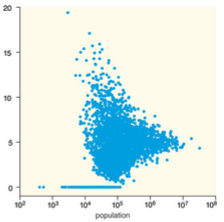
\includegraphics[width=2in]{figures/demoivre-fig.png}
\caption{Variabilidad en función de la población}

\end{figure}

El gráfico muestra la variabilidad en función de la población la forma triangular es típica, los casos con pocas muestras tienen una variabilidad mucho mayor que otros con una población mucho mayor.
Eventualmente alguien hizo los estudios adecuados y estos arrojaron que por el contrario las escuelas con mayor cantidad de alumnos tenían un mejor rendimiento académico, esto se puede explicar en función de tener una mayor cantidad de docentes y de que los mejores docentes en general quieren ir a las escuelas mas grandes.

\begin{figure}[!htb]
\centering
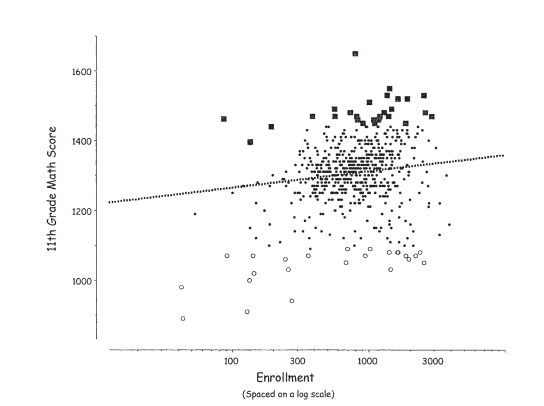
\includegraphics[width=3in]{figures/demoivre-fig2.png}
\caption{Rendimiento de alumnos del 11vo grado}

\end{figure}

Finalmente la fundación Gates dio marcha atrás y volvió a reintegrar las escuelas con muchos alumnos que habían sido divididas en varias escuelas menores. En total se gastaron miles de millones de dólares y solamente por el desconocimiento de una simple ecuación.

El ataque de de Moivre nunca ha cesado, hoy en día se publican todo el tiempo estudios en los cuales se evidencia el desconocimiento de la ecuación. Recientemente alguien publicó una lista de las ciudades mas seguras en EEUU y, como es de esperar, el listado estaba dominado por ciudades con menos de 500.000 habitantes. Lamentablemente es probable que esto nunca tenga solución.

\subsection{Frecuentistas vs Bayesianos}

De la sección anterior hemos aprendido que cuando tenemos pocos datos la variabilidad de los mismos es mayor que cuando tenemos muchos datos, en pocas palabras cuantos mas datos tenemos mas confiable es nuestra estadística y comparar estadísticas de datos con diferentes espacios muestrales suele ser una idea peligrosa. Esto nos lleva a introducir las dos grandes corrientes de pensamiento dentro de la estadística que son la corriente frecuentista y la corriente bayesiana.

La diferencia básica entre el punto de vista frecuentista y el punto de vista bayesiano radica en la información necesaria para obtener datos estadísticos. Para un frecuentista las estadísticas surgen de los datos mismos mientras que para un bayesiano las estadísticas surgen de la combinación de los datos y un cierto conocimiento a-priori sobre los mismos.

Para un frecuentista $5/10$ y $1000/2000$ son lo mismo: 0.5 para un bayesiano son cosas muy diferentes...

\begin{figure}[!htb]
\centering
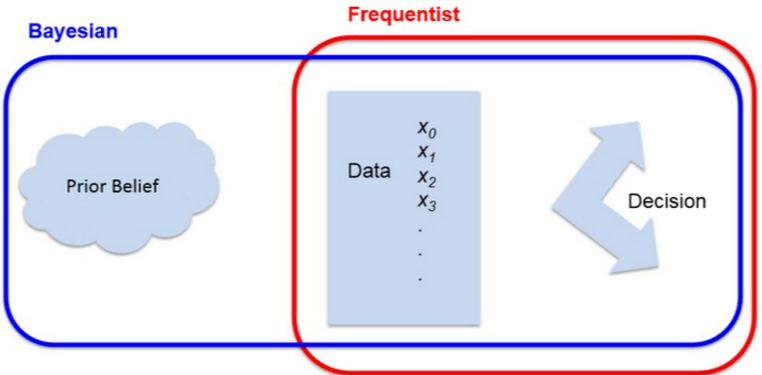
\includegraphics[width=3in]{figures/bayes-fig-1.png}
\caption{Frecuentistas vs Bayesianos}

\end{figure}

Consideremos un ejemplo muy simple: en el primer partido de la temporada un jugador de basket intenta tres triples y logra meter los tres. ¿Es lógico suponer que su efectividad en triples a lo largo de la temporada será del 100\% ?. Para un frecuentista la respuesta es "sí" ya que con los datos que tenemos el porcentaje de triples del jugador es 3/3 y por lo tanto no tenemos mas que suponer que su porcentaje durante la temporada será el mismo. Para un bayesiano esto no es así ya que tenemos que tener en cuenta el porcentaje de triples a-priori de un jugador de basket, supongamos que el porcentaje promedio de triples de todos los jugadores que juegan en la misma posición es de un 52\%, de acuerdo a la filosofía bayesiana la predicción para el jugador durante la temporada será de 52\% mas un pequeño epsilon por la evidencia que tenemos al verlo meter los primeros 3 de 3 intentos en su primer partido. 

Este sencillo ejemplo nos enseña varias cosas: de acuerdo a la filosofía bayesiana la probabilidad de un evento está dada por la probabilidad a-priori del mismo y la evidencia que tenemos (observaciones), cuanta mas evidencia tenemos mas podemos desviarnos de nuestro conocimiento a-priori. 

Veamos un segundo ejemplo: tenemos un test que tiene un 99\% de efectividad para detectar si alguien es pelirrojo. Si el test nos da positivo, ¿cuál es la probabilidad de que seamos pelirrojos?. Para un frecuentista la probabilidad es del 99\% y no hay mas discusión al respecto y es probable que ésta sea la respuesta mas popular para el público en general, al fin y al cabo el test tiene 99\% de efectividad. Para un bayesiano es necesario saber cuál es la probabilidad a-priori, es decir la probabilidad de que alguien sea pelirrojo independientemente del test. Supongamos que se sabe a-priori que uno de cada 100 individuos es pelirrojo. Con esa información podemos pensar la respuesta bayesiana a nuestra pregunta. Tenemos 100 personas, una de ellas pelirroja, les hacemos el test y como el porcentaje de eficiencia es del 99\% sabemos que le va a dar mal a una persona. Supongamos que al que es pelirrojo el test le da bien, es decir que le dice "usted es pelirojo" de los otros 99 hay 1 al cual el test le va a decir incorrectamente que es pelirrojo. En definitiva tenemos 2 respuestas de tipo "usted es pelirojo" y solo 1 de esas 2 personas realmente lo es, por lo tanto la probabilidad de ser pelirojo si el test nos da positivo es del 50\%, bayesian magic.

Formalmente acabamos de aplicar de forma intuitiva el teorema de Bayes:

\begin{myequation}
P(A|B) = \frac{P(B|A)P(A)}{P(B)}
\end{myequation}

Este teorema rige todo el proceso de inferencia bayesiana y de alguna forma se encuentra hard-codeado en el cerebro humano ya que incluso aquellos que jamás han oído hablar del mismo lo pueden aplicar cuando la situación es evidente, por ejemplo en el caso de nuestro jugador de basket. Verifiquemos si el teorema se cumple para nuestro test de pelirrojicidad.

P(A|B) es la probabilidad de ser pelirrojos si el test nos da positivo que es lo que queremos averiguar.

P(B|A) es la probabilidad de que el test nos de positivo si somos pelirrojos es decir 0.99

P(A) es la probabilidad de ser pelirrojos en general: 0.01

P(B) es la probabilidad de que el test nos de positivo en general intuitivamente podemos razonar que es 2/100 ya que le dará positivo al que es pelirrojo y a uno que no es dado que el test no es infalible. Esto lo podemos comprobar calculando:

P(B) = P(B|A)P(A) * P(B|not A) P(not A)

P(B|not A) es la probabilidad de que el test de positivo si no somos pelirrojos: 0.01
P(not A) es la probabilidad de no ser pelirrojos es decir 0.99

P(B) = 0.99 * 0.01 + 0.01 * 0.99 = 0.0198 que es el 2/100 que habíamos calculado.

Entonces:

P(pelirrojo+) = P(test+|pelirrojo)P(pelirojo)/P(test+) = 0.99 * 0.01 / 0.02 = 0.5

De los dos ejemplos que hemos visto podemos concluir que en una persona promedio el cerebro a veces funciona de forma frecuentista y a veces de forma bayesiana, en el caso del basketbolista casi todos pensamos de forma bayesiana pero en el caso del test de pelirrojicidad(?) la gran mayoría de la población comparte el pensamiento frecuentista.

La aproximación al pensamiento bayesiano automáticamente nos lleva a pensar varios problemas de una forma diferente. Veamos un tercer caso. Le tomamos a un grupo de personas un examen de 10 preguntas de cultura general y obtenemos los resultados. Ahora al mismo grupo de personas le tomamos un segundo examen de 10 preguntas de cultura general pero diferente al primero. ¿Cuál sería una buena forma de estimar el resultado para cada persona?

La aproximación frecuentista al problema es estimar para cada persona el mismo resultado que el examen anterior, si alguien respondió bien 8 preguntas estimamos que va a volver a responder bien 8 preguntas. Esto es lógico pero desde el punto de vista bayesiano es incorrecto. Para una respuesta bayesiana el resultado del examen anterior es la "evidencia", necesitamos además un cierto conocimiento a-priori y a falta de otra cosa podemos usar el promedio de los resultados de todos los exámenes ($\mu$). La predicción entonces será de la forma $e2 = \lambda \mu + (1-\lambda) e1$ siendo $\lambda$ un parámetro que regula el peso de nuestro conocimiento a-priori y nuestra evidencia. Resulta ser que con $\lambda = 0.5$ la predicción del resultado del segundo examen es mejor que la que haríamos con la filosofía frecuentista.

\subsubsection{Estimación Bayesiana con la Distribución Beta}

Para formalizar un poco la forma de usar la filosofía bayesiana vamos a ver un método de partiendo de una cierta distribución de probabilidades a-priori ir actualizándola en función de la evidencia que observamos. Para hacer esto vamos a usar la distribución Beta. La distribución beta es frecuentemente ignorada o descripta de formas muy complejas sin necesidad, lo que la distribución en realidad mide es una distribución de probabilidades y por eso es muy interesante desde el punto de vista bayesiano.

A modo de ejemplo consideremos el problema de estimar el porcentaje de triples para la presente temporada para un cierto jugador. Sabemos que para la posición en la que el jugador juega el porcentaje promedio de triples es  0.38 con una desviación standard de 0.11 (varianza = 0.0121). La distribución beta tiene dos parámetros: $\alpha$ y $\beta$ que tenemos que encontrar antes de poder usarla.

En primer lugar la varianza se puede expresar en función del promedio como:

$$\sigma^2 = \frac{\mu (1-\mu)}{\alpha + \beta +1}$$

Si queremos $\mu=0.38$ y $\sigma^2=0.0121$ entonces calculamos:

$$\alpha + \beta = \frac{\mu(1-\mu)}{\sigma^2}-1 = \frac{.38 (1-.38)}{.0121}-1 = 18.47$$

Y conociendo el total para $\alpha+\beta$

$$\alpha = \mu(\alpha+\beta) = .38 (18.47) = 7.01$$
$$\beta = (1-\mu)(\alpha + \beta) = 11.45$$

\begin{figure}[!htb]
\centering
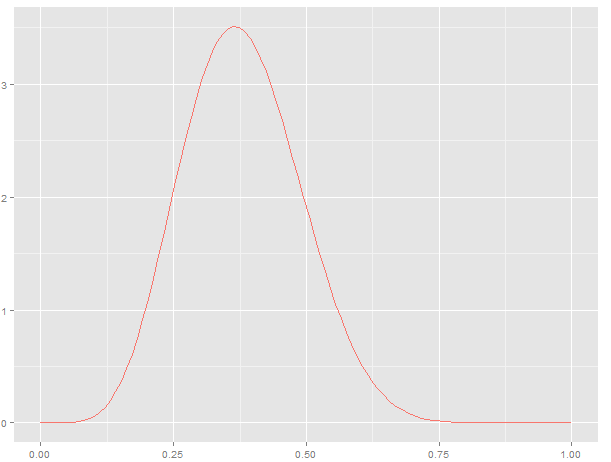
\includegraphics[width=4in]{figures/beta-fig-1.png}
\caption{Distribución Beta con $\alpha=7.01$ y $\beta=11.45$}

\end{figure}

Como podemos ver la distribución beta cumple razonablemente con lo que necesitamos, tiene promedio 0.38 y desviación standard 0.11. El promedio de la distribución beta es $\frac{\alpha}{\alpha+\beta}$

El gran truco de la distribución beta es que resulta sumamente sencillo actualizarla en función de nueva evidencia. 

$$\beta_2 = \beta_1(\alpha + hits , \beta + misses)$$

Suponiendo que nuestro jugador mete 3 triples seguidos nuestra nueva distribución beta es:

$$beta_2(7.01+3,11.45+0)$$

Si calculamos el promedio ahora tenemos $$10.01/10.01+11.34=0.46$$ notemos que nuestra predicción para el jugador en la temporada ahora es 0.46, bastante mejor que 0.38 pero lejos de un 100\% que sería la predicción frecuentista.

Supongamos que luego de varios partidos nuestro jugador mete 21 de 50 triples. Ahora el promedio es:

$$21+7.01/ (11.45+7.01+50)=0.409$$

\begin{figure}[!htb]
\centering
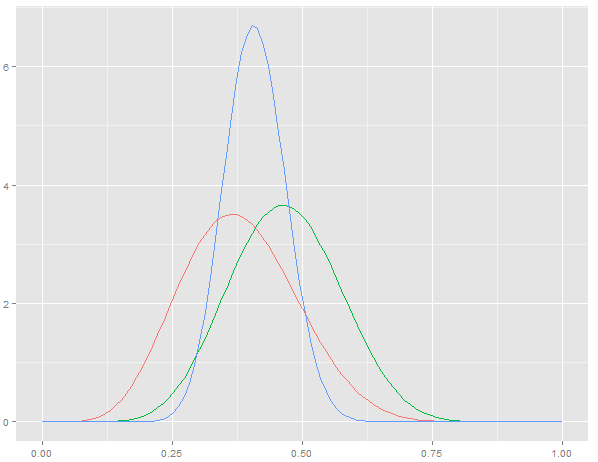
\includegraphics[width=4in]{figures/beta-fig-2.png}

\caption{Las tres distribuciones beta}
\label{fig:tresbeta}
\end{figure}

La figura ~\ref{fig:tresbeta} muestra las tres distribuciones. La roja es nuestra distribución a-priori con promedio 0.38, la verde es la distribución luego de 3 triples consecutivos, tiene promedio 0.46 la azul es la distribución luego de ver al jugador intentar 50 triples con los 21 aciertos mencionados. Observemos que a medida que agregamos evidencia la desviación standard disminuye es decir que cada vez estamos mas convencidos de cual será el porcentaje de triples del jugador durante la temporada.

La distribución beta simplifica enormemente el análisis bayesiano de las probabilidades en base a una cierta distribución a-priori y la evidencia que vamos observando. Es tan simple que muchas veces nadie cree que la estimación puede surgir de una cuenta tan sencilla como agregar los casos exitosos a $\alpha$ y los casos no exitosos a $\beta$ y calcular $\alpha/(\alpha+\beta)$ para estimar el promedio. 

\begin{verbatim}
// We hired a Data Scientist to analyze our Big Data
// and all we got was this lousy line of code.
float estimate = (successes + 78.7) / (total + 303.5);
\end{verbatim}

La filosofía bayesiana da lugar al algoritmo de clasificación \textit{naive bayes} que veremos mas adelante y a las redes bayesianas, y de acuerdo a quienes profesan esta corriente, es la explicación para todo lo que ocurre en el universo!

\subsection{La Única Ley sin Explicación}
Es muy difícil explicar una ley que no se cumple siempre pero casi y que no tiene ningún tipo de demostración aceptada pero que al mismo tiempo ha llegado a aceptarse como prueba en pericias judiciales. Estamos hablando de la ley de Benford.
Esta ley postula lo siguiente: "En un conjunto de datos numéricos la distribución del primer dígito de cada número no es uniforme sino que los dígitos mas pequeños aparecen en mayor proporción que los mas grandes"
En otras palabras estamos diciendo que si tenemos un conjunto de datos numéricos y contamos la frecuencia del primer dígito de cada número vamos a encontrar que el dígito 1 es mucho mas frecuente que el 2, este es mas frecuente que el 3 y así sucesivamente.

\begin{figure}[!htb]
\centering
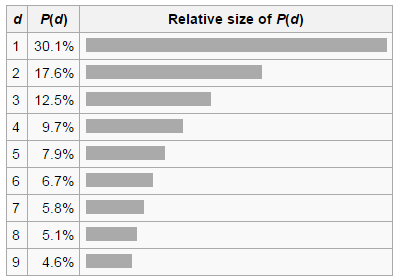
\includegraphics[width=3in]{figures/benford-fig.png}
\caption{Distribución de los dígitos según la ley de Benford}

\end{figure}

Como vemos en el gráfico la distribución es logarítmica: un 30\% de los números en nuestro set de datos empezarán con unos, un 17.6\% con 2 y así sucesivamente hasta el 9 que debería encabezar un 4.6\% de los números.
Esta ley parece no tener sentido alguno sin embargo es válida para una enorme cantidad de sets de datos, por ejemplo la altura de los edificios más altos del mundo, la distancia entre el Sol y las estrellas más cercanas, etc.

La ley de Benford suele cumplirse con tanta regularidad que se ha aceptado como pericia para demostrar fraudes cuando la presentación de ciertos valores numéricos por una de las partes no ajusta a la distribución esperada de acuerdo a la ley de Benford.Para transacciones financieras la ley de Benford se cumple con una efectividad casi asombrosa.

\begin{figure}[!htb]
\centering
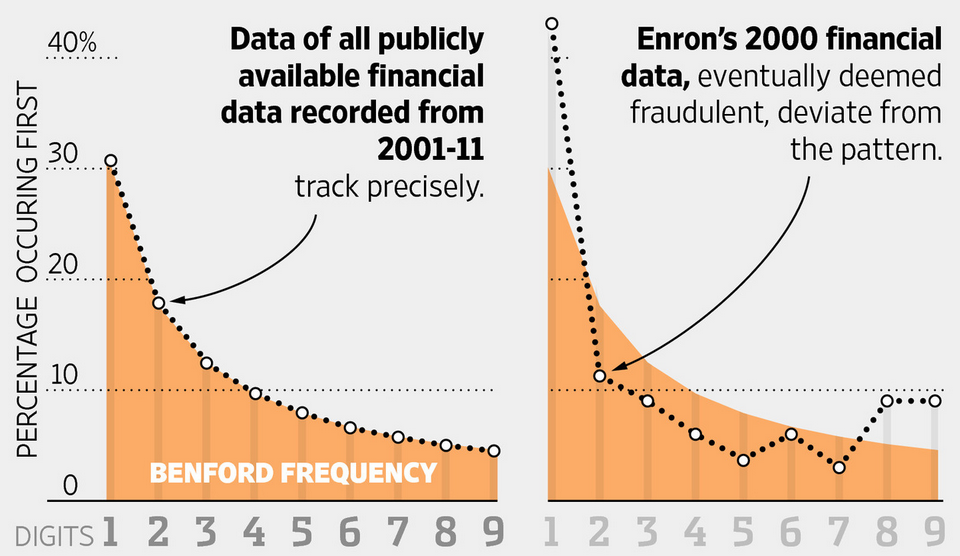
\includegraphics[width=4in]{figures/benford-enron-fig.png}

\caption{La ley de Benford en transacciones financieras públicas vs los datos entregados por Enron.}
\label{fig:benford}
\end{figure}

En la figura ~\ref{fig:benford} a la izquierda vemos como la información financiera pública ajusta casi de forma perfecta a la ley de Benford, en la derecha vemos los valores para los informes presentados en 2000 por Enron y que eventualmente se encontró de caracter fraudulento, ¡los números no coinciden!

Hay varios intentos de explicar la ley de Benford pero ninguno ha sido aceptado como lo suficientemente riguroso, aunque parezca mentira esta ley no tiene explicación ni demostración, simplemente se cumple.

\subsection{Skewness}

El fenómeno conocido como "skewness" se da cuando la distribución de las clases en nuestro set de datos está muy desbalanceada. Consideremos el ejemplo típico de una base de datos con emails rotulados como spam o no-spam que queremos usar como set de entrenamiento para un clasificador que nos permita predecir si un email no rotulado es spam o no. En el set de entrenamiento vamos a tener muchos mas emails rotulados como no-spam que como spam ya que afortunadamente el spam es sólo un pequeño porcentaje del total del volumen de emails que circulan diariamente. Por ejemplo podríamos tener un set de entrenamiento en el cual un 1\% de los mensajes están rotulados como spam. 

Este desbalanceo es peligroso ya que puede afectar seriamente el funcionamiento de nuestros algoritmos. Como ejemplo consideremos un algoritmo que simplemente predice "no-spam" para cualquier texto que se le presente. De acuerdo con nuestro set de entrenamiento este algoritmo tendrá una precisión del 99\% y sin embargo no hace absolutamente nada. 

La performance de una predicción muy simple la llamaremos "baseline", cuando el set de datos está muy desbalanceado el baseline suele fijar la vara muy alta por lo que hay que tomar con mucho cuidado el resultado de nuestros algoritmos.

Hay varias formas de combatir el skewness, una es realizar un muestreo estratificado del set de datos para asegurarnos que tenemos un cierto porcentaje de datos de cada clase, esto va a ayudar a los algoritmos a distinguir mejor entre las clases que existen sin introducirles el bias de saber que una de las clases es mucho mas importante que la otra.

En otros casos es posible asignar pesos a los errores de clasificación y podemos decir que el error de clasificar un mail normal como spam es mucho mas alto que el de clasificar un spam como normal, de esta forma el algoritmo va a tender a tener mas cuidado en la clasificación que realice. 
Este tema aparece muy frecuentemente y la forma de solucionarlo es dependiente del algoritmo que usemos por lo que será siempre un factor fundamental a considerar en el análisis exploratorio de nuestros datos. 


\section{Algoritmos Aleatorizados}
Los algoritmos aleatorizados son aquellos que en algún momento toman alguna decisión al azar. Podemos dividirlos en dos grandes familias:
\paragraph{Algoritmos tipo Montecarlo} Estos algoritmos siempre terminan en una cantidad de tiempo acotada pero pueden no encontrar la solución óptima. En su forma mas básica podemos decir que prueban soluciones al azar y se quedan finalmente con la que optimiza una cierta función, ya sea maximizándola o minimizándola para el conjunto de soluciones probadas.
\paragraph{Algoritmos tipo Las Vegas} Estos algoritmos siempre encuentran la solución óptima pero, con una cierta probabilidad, pueden tardar mucho tiempo en encontrarla.

A modo de ejemplo veamos un algoritmo de tipo Montecarlo para calcular el valor de $\pi$. La idea es muy simple: vamos a tener un cuadrado de lado $2r$ y un círculo inscripto dentro del mismo de radio $r$. Nuestro algoritmo va a generar puntos al azar dentro del cuadrado y va a verificar si caen dentro o fuera del círculo, sabiendo que si caen dentro entonces $x^2+y^2<r^2$.
Luego de simular millones de puntos tenemos la cantidad de puntos totales y la cantidad de estos puntos que cayeron dentro del círculo y a partir de estas cantidades podemos estimar el valor de $\pi$

\begin{figure}[!htb]
\centering
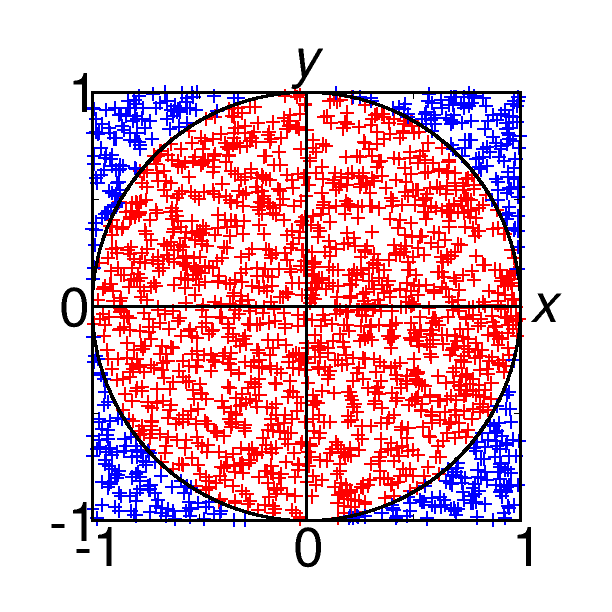
\includegraphics[width=2in]{figures/pimc-fig.png}
\caption{Calculando $\pi$ mediante Montecarlo.}

\end{figure}

El área del círculo es $\pi*r^2$ y el área del cuadrado es $(2r)^2$ por lo tanto si dividimos el área del círculo por el área del cuadrado obtenemos:

$$\frac{\pi*r^2}{(2r)^2)}=\frac{\pi}{4}$$

Por lo tanto si elegimos $N$ puntos al azar dentro del cuadrado entonces $M=N*\pi/4$ van a caer dentro del círculo. Como nuestra simulación cuenta la cantidad M y N podemos calcular 

$$pi \approx \frac{4M}{N}$$

\begin{algorithm}
 \KwData{r: circle radius, N:number of iterations}
 \KwResult{pi}
M=0\;N=0\;
 \For{i in (1..N)}{
 x = rand(0,2r)\;
 y = rand(0,2r)\;
 \If{$x^2+y^2<r^2$}{
  M= M +1
   }
}
pi = 4M/N\;
\caption{Algoritmo tipo Montecarlo para calcular pi}
\end{algorithm}

Consideremos ahora el problema de calcular el promedio en bytes del tamaño de todas las páginas web. Claramente no es factible simplemente tomar todas las páginas web y calcular el promedio de su tamaño en bytes. Un algoritmo de tipo Montecarlo puede aproximar esta cantidad simplemente tomando una cierta cantidad fija de páginas al azar, por ejemplo un millón y calculando su promedio. De acuerdo a la ley de los grandes números cuanto mayor sea el tamaño de la muestra que tomamos mas cerca va a estar nuestra estimación de converger a la solución verdadera.

\subsection{Algoritmo de Fermat}
El algoritmo de Fermat es un algoritmo de tipo Montecarlo muy simple para determinar si un número es primo, está basado en el pequeño teorema de Fermat que dice:

\begin{theorem}[Fermat]
si $p$ es primo entonces para $$ 0<a<p$$
$$a^{p-1} = 1 \pmod p$$
\end{theorem}

El algoritmo entonces simplemente genera valores al azar para $a$ y si todos los valores probados cumplen con el teorema entonces el número es primo.

\begin{algorithm}
\KwData {p,iterations}
\KwResult{composite if n is composite, otherwise probably prime}
\For {i in (1..iterations)}{
  \If{$a^{p-1} \bmod p \ne 1$} {
  return composite\;
  }
}

return probably prime\;
\caption{Algoritmo de Fermat}
\end{algorithm}

\subsection{Algoritmo de Miller-Rabin}
El algoritmo de MillerRabin es un algoritmo tipo Montecarlo para probar si un número es primo o no, es mas eficiente que el algoritmo de Fermat en el sentido de que es menos probable que un número que no es primo pase el test.

\begin{algorithm}
\KwData { $n > 2$, an odd integer to be tested for primality\;
       k, a parameter that determines the accuracy of the test\;}
\KwResult{Output: composite if n is composite, otherwise probably prime}
write $ n-1$ as $2^s*d$ with d odd by factoring powers of 2 from $n-1$\;
\For {i in (1..k)}
   pick a randomly in the range $[2, n-1]$\;
  $ x = a*d \bmod n$\;
  \If {$x = 1$ or$ x = n-1$} {do next LOOP}
   \For {r=1 .. s-1} {
     $ x = x^2 \bmod  n$
     \If{ x = 1} {return composite}
     \If {x = n-1 } {do next LOOP}
   }
   return composite\;
return probably prime\;
\caption{Algoritmo de Miller-Rabin}
\end{algorithm}

\subsection{Random Walks}
Un Random Walk es un recorrido al azar, por ejemplo podemos generar un random walk al azar en dos dimensiones comenzando en una cierta coordenada al azar (X,Y) y luego desplazándonos a X+1, X-1, Y+1 o Y-1.

\begin{figure}[!htb]
\centering
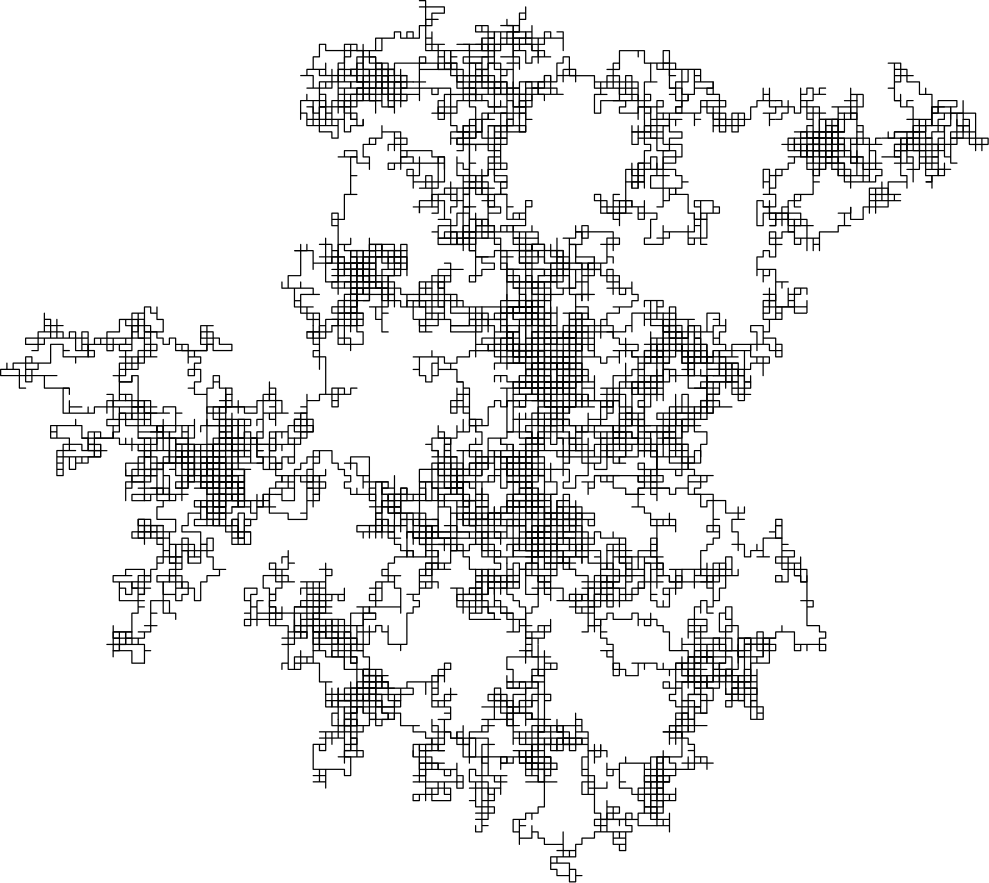
\includegraphics[width=3in]{figures/random-walk-fig-1.png}
\caption{Random Walk en 2d (25000 iteraciones).}

\end{figure}

Los Random Walks son extremadamente útiles para simular todo tipo de procesos y estimar luego parámetros que son difíciles de calcular analíticamente o que no sabemos calcular.

\subsection{Markov Chains}
Una cadena o proceso de Markov es un grafo dirigido en donde cada nodo representa un estado y cada arista representa un transición de un estado a otro. Cada arista lleva un rótulo indicando su probabilidad. La suma de todas las aristas salientes de un nodo debe ser 1.

\begin{figure}[!htb]
\centering
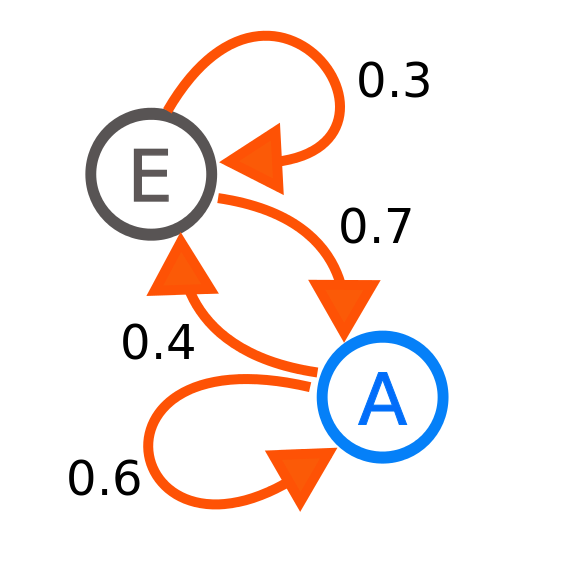
\includegraphics[width=2in]{figures/markov-chain-fig-1.png}
\caption{Cadenas de Markov.}

\end{figure}

Las cadenas de Markov pueden usarse para modelar todo tipo de procesos, por ejemplo podemos modelar información meteorológica usando como nodos los diferentes estados del tiempo (soleado, parcialmente nublado, nublado, lluvia, tormenta) y cada arista representa la probabilidad de pasar de un estado a otro.

\begin{figure}[!htb]
\centering
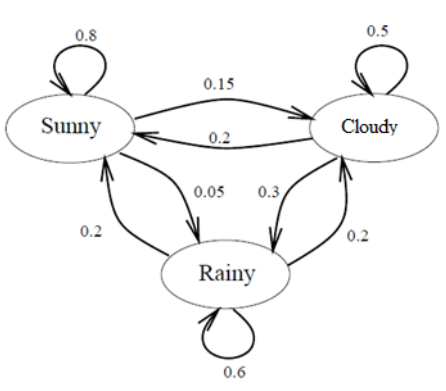
\includegraphics[width=3in]{figures/markov-chain-fig-2.png}
\caption{Proceso de Markov para el pronóstico del tiempo.}

\end{figure}

Como podemos ver si el día está soleado lo mas probable es que mañana también esté soleado y lo menos probable es que llueva.
Hay muchísimas cosas que podemos hacer con una cadena de Markov de forma analítica pero es destacable que sin tener absolutamente ningún conocimiento sobre procesos de Markov podemos responder prácticamente cualquier pregunta mediante una simulación de tipo Montecarlo.

Como ejemplo supongamos que queremos saber cuál es la probabilidad de que dentro de un mes tengamos tres días soleados. Realizamos un Random Walk comenzando en cualquier estado al azar y probabilísticamente vamos moviéndonos de un estado a otro hasta simular los 30 días, luego simplemente contamos cuantas veces aparecen tres estados "sunny" consecutivos, esto lo podemos repetir $n$ veces y calcular un promedio para mayor efectividad siempre amparados en el poder de la ley de los grandes números.

Realizar la simulación es muy simple, por cada estado(nodo) generamos un número random entre 0 y 1 y nos fijamos a que transición corresponde. Por ejemplo supongamos que estamos en "sunny" tenemos probabilidad 0.05 de ir a "rainy", 0.15 a "cloudy" y 0.8 de seguir en "sunny" generamos un número entre 0 y 1 al azar y si el número es menor o igual a 0.8 entonces el próximo estado es "sunny" si el número es mayor a 0.8 y menor a 0.95 el próximo estado es "cloudy" y si el número es mayor a 0.95 el próximo estado es "rainy" como podemos ver esto es acorde con la probabilidad de cada arista en nuestro grafo.

\subsubsection{Modelando Lenguajes como Procesos de Markov}
Una de las aplicaciones mas sorprendentes de un proceso de Markov es el modelado de un lenguaje. Podemos procesar una gran cantidad de textos y contabilizar la cantidad de veces que un caracter aparece luego de otro, de esta forma una vez procesados todos los textos podemos tener un grafo en el cual cada nodo representa un caracter y las transiciones representan la probabilidad de que un caracter aparezca luego de otro. Un random walk en este grafo genera texto al azar imitando las propiedades de los textos que procesamos.
El modelo puede mejorarse si en lugar de caracteres individuales tomamos grupos de $n$ caracteres que llamaremos \textit{n-gramas} por ejemplo podemos registrar por cada 3 caracteres la probabilidad del próximo caracter, en nuestro grafo cada nodo representa ahora cuáles son los $n$ caracteres anteriores y las transiciones representan cuál será la probabilidad del próximo caracter.
A modo de ejemplo procesamos todas las obras de Shakespeare y luego usando $n=10$ simulamos un random walk sobre el grafo el resultado es el siguiente:
\begin{verbatim}
First Citizen:
Nay, then, that was hers,
It speaks against your other service:
But since the
youth of the circumstance be spoken:
Your uncle and one Baptista's daughter.

SEBASTIAN:
Do I stand till the break off.

BIRON:
Hide thy head.

VENTIDIUS:
He purposeth to Athens: whither, with the vow
I made to handle you.

FALSTAFF:
My good knave.

MALVOLIO:
Sad, lady! I could be forgiven you, you're welcome. Give ear, sir, my doublet and hose and leave this present death.

Second Gentleman:
Who may that she confess it is my lord enraged and forestalled ere we come to be a man. Drown thyself?

APEMANTUS:
Ho, ho! I laugh to see your beard!
\end{verbatim}

Como podemos apreciar el texto no solamente tiene sentido sino que luce como Shakespeare aunque haya sido generado completamente al azar por un simple programa. Esto muestra el enorme poder de los procesos de Markov para entender una secuencia de eventos y la increíble efectividad de un simple Random Walk tipo Montecarlo como proceso generativo. Es por esto que muchos compresores de texto utilizan modelos de Markov para modelar el archivo a comprimir logrando niveles de compresión excelentes.

\subsection{Hill Climbing}
Hill Climbing es una familia de algoritmos con un principio muy simple: comenzar con una solución al azar, proponer un cambio y aceptarlo solamente si el cambio mejora la solución. Podemos decir que se trata de una meta-heurística ya que se trata de un algoritmo para construir otros algoritmos.

\begin{algorithm}
create a random solution s\;
\For {i in (1..iterations)} {
  propose an alternative solution (s')\;
  \If {s' better than s} {
    s = s'\;
  }
}
return s\;
\caption{Hill Climbing}
\end{algorithm}

Para transformar una solución en otra se tiene que realizar lo que se denomina un "cambio local" es decir un pequeño cambio en la solución. Por ejemplo supongamos que queremos minimizar la función $2x^2-3x+2$ podemos comenzar con un cierto valor de $x$ al azar generar un $\epsilon$ al azar positivo o negativo y proponer la solución $x+\epsilon$ aceptando este valor solamente si la función ha disminuido entre una solución y la otra. Eventualmente este simple proceso de Hill-Climbing va converger al mínimo de la función.

El proceso de Hill-Climbing no es ni mas ni menos que un algoritmo "greedy"  y no funciona si la función que queremos maximizar o minimizar tiene máximos o mínimos locales ya que una vez que comenzamos en una cierta solución al azar vamos a poder llegar únicamente al máximo o mínimo local mas cercano a la misma. Para evitar quedar atrapados en extremos locales usamos una versión mejorada de Hill-Climbing que se denomina algoritmo de Metrópolis-Hastings.

\subsection{El Algoritmo Metrópolis-Hastings}

La variante que introducimos en el algoritmo de Metrópolis-Hastings es aceptar una solución que empeora nuestro resultado con una pequeña probabilidad. 

\begin{algorithm}
create a random solution s\;
\For {i in (1..iterations)} {
  propose an alternative solution (s')\;
  \If {s' better than s or if $random(0,1) \leq p$ (a small number)} {
    s = s'\;
  }
}
return s\;
\caption{Metrópolis-Hastings}
\end{algorithm}

La heurística de Metrópolis-Hastings mejora el resultado de Hill-Climbing para funciones que tienen mínimos y máximos locales pero en general no se usa sino como parte de un algoritmo mas avanzado denominado "Simulated Annealing"

\subsection{Simulated Annealing}

Simulated Annealing (SA) es un meta-algoritmo extremadamente poderoso que se usa para aproximar soluciones a todo tipo de problemas muy difíciles de solucionar por otros métodos, es uno de los algoritmos mas usados para aproximar problemas que se sabe son NP-Completos. 
La idea es partir del algoritmo Metrópolis-Hastings e ir variando la probabilidad de aceptar una solución que empeora nuestro resultado. Al principio cuando recién empezamos a explorar el espacio de soluciones queremos aceptar soluciones que no mejoran el resultado final con una cierta probabilidad "$p_1$" luego se supone que nuestra solución va mejorando y queremos que esta probabilidad vaya disminuyendo hasta llegar a ser prácticamente cero en las últimas iteraciones. Esto lo logramos variando un parámetro que llamaremos la "temperatura" del algoritmo.

\begin{figure}[!htb]
\centering
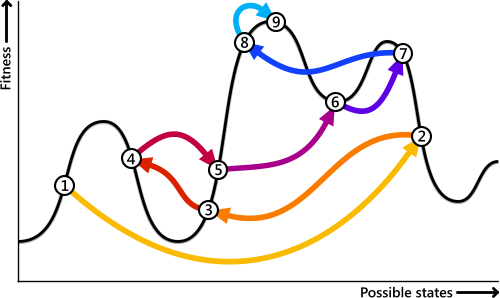
\includegraphics[width=3in]{figures/sa-fig.png}
\caption{Ejemplo de Simulated Annealing en 9 iteraciones.}

\end{figure}

Supongamos que estamos minimizando una cierta función $f(s)$; al igual que siempre vamos a comenzar con una cierta solución al azar $s$ y proponer un pequeño cambio para generar la solución $s'$. 

Tenemos que definir entonces una función que nos diga la probabilidad de aceptar a esta nueva solución $P(s,s',T)$ la probabilidad de aceptar $s'$ depende de $s$,$s'$ y la temperatura $T$. Esta función nos debe devolver una probabilidad siempre, incluso cuando $s'$ es mayor a $s$ es decir una solución peor.Además queremos que cuando $T\to0$, $P$ tienda a cero. Si $s'>s$ cuando $T=0$ el algoritmo se convierte en Hill-Climbing aceptando únicamente una solución alternativa si mejora el resultado actual. 
Una posible forma de definir la función de probabilidad P es:

\begin{displaymath}
   P(s,s',T) = \left\{
     \begin{array}{lr}
       1 :  s'<s\\
        \exp(-(s'-s)/T): otherwise \\
     \end{array}
   \right.
\end{displaymath} 

El algoritmo de Simulated Annealing quedaría entonces definido de la siguiente forma:

\begin{algorithm}
create a random solution s\;
\For{T in Tmax..0 step tstep} {
  propose an alternative solution $s'$\;
\If {random(0,1) $\leq$ $P(s,s',T)$} {
    s = s'\;
  }

}
return s\;
\caption{Simulated Annealing}
\end{algorithm}

La temperatura inicial $Tmax$ y el grado en el cual vamos disminuyendo la temperatura $tstep$ determinan la cantidad de iteraciones que vamos a realizar. Alternativamente podemos usar como parámetro la cantidad de iteraciones y $Tmax$ y calcular cuál es el step para ir desde $Tmax$ a 0 en dicha cantidad de iteraciones.

Simulated Annealing es un algoritmo muy importante ya que permite optimizar todo tipo de problemas conociendo únicamente como generar una solución alternativa a partir de cualquier otra solución (local change). Se usa para la aproximación de problemas como el problema del viajante y otros tipos de problemas muy complejos para los cuales no existe un método eficiente para llegar a la solución óptima. Es crítico en estos algoritmos determinar los parámetros correctos para converger a la mejor solución posible, es común ir probando diferentes valores de temperatura y cantidad de iteraciones hasta llegar a la mejor solución posible. 

\section{MCMC}

Vamos a empezar esta sección con un curioso ejemplo. Supongamos que queremos encuestar a la población con respecto a una pregunta en la cual suponemos que la mayoría de la gente va a mentir. Por ejemplo ¿Le gusta Arjona?. Vamos a proponer un algoritmo para poder realizar la encuesta:

\begin{enumerate}
\item Cada persona tira una moneda.
\item Si sale cara la persona responde honestamente.
\item Si sale seca la persona lanza una segunda moneda.
\item Si la segunda moneda es cara entonces responde "Si".
\item Si la segunda moneda es seca entonces responde "No"
\end{enumerate}

Con este sencillo algoritmo nadie necesita mentir ya que es imposible discernir individualmente si una respuesta de "Si" fue honesta o simplemente el resultado de la segunda moneda. Es decir que podemos confiar en los resultados.

El problema es que nuestros resultados tienen ahora ruido que nosotros mismos hemos introducido intencionalmente. Supongamos que 100 personas responden usando el algoritmo propuesto y obtenemos 35 respuestas "Si". 

De nuestras 100 personas podemos esperar que 50 hayan sacado cara en la primera moneda y hayan respondido honestamente. De los restantes 50 podemos esperar 25 respuestas "Si" y 25 respuestas "No". Por lo tanto de los otros 50 tiene que haber 10 respuestas afirmativas y eso nos permitiría afirmar que la probabilidad de que a una persona le guste Arjona es 10/50 =  0.2. 

Podemos ver que nuestro algoritmo ha disminuido el espacio muestral a cambio de privacidad en las respuestas, pero a menor espacio muestral tenemos mayor incertidumbre, ciertamente sería un error afirmar categóricamente que al 20\% de la población le gusta Arjona (el cielo se apiade).

Lo que nos interesa es la \textit{distribución} de probabilidad de p(arjona), en el enfoque Bayesiano queremos averiguar la distribución a-priori. El algoritmo que nos permite hacer esto es MCMC (Markov Chain Monte-Carlo).

Para entender MCMC pensemos una sencilla solución a nuestro problema. Podemos tirar un valor al azar para p(arjona) y simular 100 experimentos usando este valor, es decir 100 simulaciones de nuestro algoritmo con las dos monedas. Si como resultado obtenemos 35 respuestas "Si" entonces \textit{aceptamos} el valor de p. Si repetimos este proceso miles de veces con valores de p aleatorios todo los valores aceptados de p nos terminan dando la distribución de la probabilidad de que a la gente le gusta Arjona:

 \begin{figure}[!htb]
 \centering
 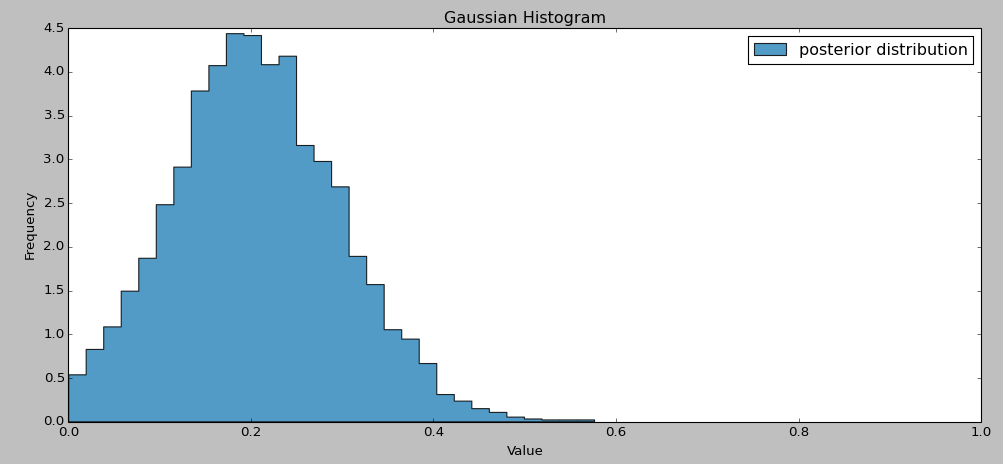
\includegraphics[width=4in]{figures/mcmc-fig-2.png}
 
 \caption{Distribución a-priori}
 \label{fig:mcmc1}
 \end{figure}

La figura ~\ref{fig:mcmc1} nos muestra el resultado de la simulación. Como podemos ver la misma está centrada en 0.2 que es el valor que habíamos calculado analíticamente pero ahora podemos ver también qué grado de incertidumbre tenemos. Podemos ver que casi con certeza el valor de p no puede ser 0.6 o mayor y que la mayoría de los valores están entre 0.05 y 0.4. Esta información es extremadamente valiosa ya que nos permite experimentar con otros espacios muestrales y algoritmos.

Lo que MCMC hace es simplemente "navegar" aleatoriamente por diferentes valores que puede tomar nuestra distribución a-priori "p" y verificar si esos valores son buenos o malos de acuerdo a la distribución a-posteriori (en nuestro caso 35/100).

Pensemos ahora el caso en el cuál tenemos no una sino varias distribuciones a-priori que queremos averiguar, el algoritmo empieza a tener problemas porque la cantidad de valores a probar crece de forma exponencial y es probable que incluso luego de millones de simulaciones no podamos converger a un valor adecuado para nuestras distribuciones. Es aquí donde aparece la verdadera inteligencia del algoritmo MCMC que no es ni mas ni menos que aplicar la heurística Metrópolis-Hastings que ya hemos visto.

El algoritmo va a empezar con ciertos valores al azar para las distribuciones desconocidas, que pueden tomarse de cualquier distribución, en nuestro caso la distribución es uniforme porque todos los valores de p son equiprobables pero podría ser una Poisson, Exponencial, etc. Una vez que el algoritmo tiene un estado "inicial" puede calcular la probabilidad a-posteriori de dicho estado. Con este dato el algoritmo ahora sugiere un cambio, es decir una variación en una de las probabilidades y calcula la nueva probabilidad a-posteriori, si es mejor a la anterior entonces el algoritmo acepta el cambio, si es peor entonces lo acepta con una probabilidad que es $p_{i}/p_{i-1}$ donde sabemos que $p_{i-1}>p_i$ ya que sino hubiesemos aceptado el cambio automaticamente. 

Siguiendo este proceso MCMC va convergiendo a los valores de las $n$ distribuciones a-priori que son mas probables y nos devuelve, igual que en nuestro caso los distintos "samples" de estas probabilidades. 

Supongamos que tenemos dos distribuciones a-priori ambas uniformes. Nuestro "espacio" es un cuadrado en dos dimensiones en donde cualquier punto del cuadrado es un par de probabilidades válido. Para cada punto de este cuadrado hay un cierto valor a-posteriori que podemos pensar como la elevación de una montaña sobre el cuadrado. El objetivo de MCMC es encontrar la montaña, por eso va navegando el cuadrado intentando subir, para encontrar los valores de p1 y p2 que maximicen la distribución a-posteriori. 

MCMC es un algoritmo extremadamente poderoso ya que nos permite a partir de los resultados observados de un cierto experimento obtener cuáles fueron las probabilidades a-priori que generaron dichos resultados con mayor probabilidad. Esto puede usarse en una gran cantidad de aplicaciones y es el algoritmo mas importante para realizar análisis de datos bayesianos. 

Habiendo explicado la intuición del algoritmo debemos aclarar que es muy complejo programar MCMC de forma eficiente por lo que recomendamos usar alguna biblioteca o función que esté bien testeada y optimizada. PyMC en Python es un buen ejemplo. 

\section{Gibbs Sampling}

Una forma de aplicar MCMC es simulanto valores de nuestro set de datos, valores nuevos no aquellos que ya conocemos. Para hacer esto tenemos que conocer la distribución de probabilidades del set de datos y no la tenemos. Los casos posibles son demasiados ya que cada punto es una variable de $n$ dimensiones en donde cada dimensión puede tomar muchos valores posibles por lo que sería imposible generar todos los casos posibles y luego tomar uno al azar de estos.

La solución para el problema de generar muestras suele ser emplear el método conocido como \textit{Gibbs sampling}, en este método vamos a elegir un dato al azar de nuestro set de datos como punto de partida, luego vamos a elegir una variable al azar (columna) y para esa variable vamos a generar un valor nuevo. El valor nuevo lo generamos en base a la distribución de probabilidades fijando las otras variables del punto seleccionado.

\section{La Unión hace la fuerza: Ensambles}

La última sección de nuestro largo capítulo introductorio la dedicamos a explicar brevemente un concepto que es fundamental en todo proceso de Data-Science: el resultado de varios algoritmos combinados casi siempre es mejor que el resultado de cualquier algoritmo individualmente.

Este concepto se ha demostrado empíricamente en muchísimas ocasiones, en el famoso concurso del premio Netflix que otorgó un millón de dólares a los ganadores el equipo ganador usó un ensamble de mas de 200 algoritmos diferentes. El mejor algoritmo de compresión hasta la fecha (PAQ) utiliza un ensamble de varios algoritmos diferentes para poder comprimir cada bit del archivo.

El principio detrás del éxito de los ensambles es muy simple: cada algoritmo explota particularmente algunas propiedades de nuestro set de datos, es decir que para diferentes datos diferentes algoritmos funcionan mejor, como lo que tenemos es un conjunto de datos la combinación de varios algoritmos suele ser la que nos de los mejores resultados. 

Mas adelante veremos diferentes métodos para crear ensambles de algoritmos y de esta forma sacar provecho de la unión de varios modelos diferentes para una solución común.

Como cierre de este capítulo que ha sido tan largo y tan extenso queremos quedarnos con los dos conceptos mas importantes que hemos visto:

\begin{enumerate}
\item Siempre es bueno conseguir mas datos a punto tal que conseguir mas datos suele ser mejor que conseguir un mejor algoritmo
\item La unión de varios algoritmos suele ser mejor que el resultado individual de cada uno de ellos.
\end{enumerate}


\chapter{Visualización}

\epigraph{The minimum we should hope for with any display technology is that it should do no harm.}{\textit{- Edward Tufte}}

En este capítulo abordamos el tema de visualizar datos, las visualizaciones son fundamentales por dos motivos: en primer lugar para entender los datos desde el punto de vista del análisis exploratorio y también para comunicar resultados como parte final del proceso de Data Science. La forma en que visualizamos en un caso u otro es completamente diferente. 

Cuando visualizamos como parte del análisis exploratorio de los datos creamos muchas visualizaciones simples sin preocuparnos demasiado por el aspecto estético de las mismas, este tipo de visualizaciones son meramente funcionales y tienen como objetivo descubrir información acerca de los datos. Mediante plots podemos entender cómo se distribuyen las variables, la relación que existe entre diferentes variables de nuestro set de datos, cuáles atributos sirven y cuáles no para la pregunta que queremos responder, podemos detectar datos anómalos, que pueden indicar errores en el proceso de obtener y depurar los datos. Podemos observar como se agrupan los datos en clusters si los representamos en 2D. En el análisis exploratorio usamos un conjunto de plots standard como herramientas que aplicamos a los datos para entenderlos.

Las visualizaciones que tienen como objetivo comunicar los resultados del proceso de Data Science son menos y el aspecto estético de las mismas es mucho mas importante. En estas visualizaciones es normal crear plots ad-hoc que sean específicos para lo que queremos comunicar o sean variantes de plots conocidos. Es fundamental que la visualización transmita la historia que queremos contar, que el público pueda entenderla y obtener a partir de ellas las conclusiones que obtuvimos en el proceso de data science que aplicamos a los datos. 

En este capítulo vamos a comentar algunas reglas básicas y fundamentales sobre visualización de datos y luego vamos a presentar los tipos de plots mas comunes comentando acerca de como usarlos. En algunos casos usaremos \textit{ggplot2} en R para crear los plots que mostramos.

\section{Principios Básicos}

\subsection{No usar tres dimensiones de forma injustificada}

Todas las visualizaciones se presentan en papel o pantallas que tienen dos dimensiones, el uso de plots de 3-d que necesariamente deben proyectarse en 2-d está desaconsejado salvo que sea absolutamente necesario. Por ejemplo el uso de plots en 3-d puede ser necesario si lo que importa es la forma que tienen ciertos objetos en el espacio tridimensional. 

En los plots en 3-d la profundidad puede producir efectos no deseados, es muy común encontrar plots tridimensionales en los cuales ciertas áreas parecen mayores que otras que son iguales simplemente por la sensación de estar mas cerca del lector. 

\subsection{El uso del plano}

La posición de los objetos en el plano es una de las fuentes de información mas importantes en un plot. En general la información en el eje $Y$ tiene mas relevancia que la información en el eje $X$, esto probablemente se deba a que asociamos el eje $Y$ con el efecto de la gravedad. Es por esto que en gráficos que muestran la evolución de una variable a lo largo del tiempo el tiempo debe ir en el eje $X$ y la variable de interés en el eje $Y$.

\subsection{Oclusión de Información}

La pauta de profundidad mas importante que podemos recibir es la oclusión, es decir cuando un objeto o parte de un objeto queda oculta detrás de otro. La información visual es que el objeto parcialmente oculto está detrás del objeto que podemos ver completo. En líneas generales esto implica que el objeto en primer plano es mas importante. 

La oclusión puede usarse en plots para relativizar la información de los objetos poniendo a aquellos que el lector debe visualizar mas tarde en un segundo plano.

\subsection{Mal uso del Plano}

Así como no debemos usar visualizaciones en 3-d cuando dos dimensiones son suficientes tampoco es recomendable usar plots en dos dimensiones cuando una simple lista en una dimensión es suficiente. 

Las listas son muy efectivas cuando el orden de los objetos en la visualización es importante, por ejemplo ordenar textos en forma alfabética ayuda a poder encontrar rápidamente un texto o etiqueta que nos interese, en contraste encontrar un nodo por su etiqueta en 2-d puede ser una tarea costosa que requiere que el usuario busque por todo el espacio de la visualización

\subsection{Capacidad de Retención}

En general la regla de 7+/-2 es una buena aproximación a la cantidad de información que el cerebro puede retener a muy corto plazo, cuando creamos visualizaciones debemos tener en cuenta esta regla para no crear una cantidad excesiva de elementos visuales que dificulten el proceso de comprensión de las mismas.

\subsection{Ceguera al cambio}

En visualizaciones que buscan comparar diferentes cosas mediante varios plots debemos tener en cuenta que en todas las personas la capacidad de detectar cambios es muy pobre cuando se centra la atención en otro objeto. Es decir que si queremos que el usuario haga una comparación debemos asegurarnos que el centro de atención de nuestra visualización esté precisamente en el objeto que cambia.

\subsection{Uso del Color}

Si bien el uso del color ayuda en muchas visualizaciones es un buen principio asegurarse que las mismas puedan entenderse correctamente en blanco y negro, esto tiene varias ventajas: en primer lugar nos aseguramos que las personas con problemas de daltonismo puedan entender la visualización correctamente, en segundo lugar nos aseguramos que nuestra visualización pueda verse correctamente en un e-reader o luego de imprimirse en B\&N. Finalmente si la visualización es efectiva en blanco y negro entonces podemos estar seguros de que el color es un elemento que ayuda a la misma y no parte de la visualización.

En la temporada 2015 la NFL estrenó uniformes nuevos para el partido entre los Jets de NY y los Bills de Buffalo, los uniformes de fuertes tonos rojos y verdes eran fáciles de distinguir en color pero lamentablemente resultaban prácticamente idénticos bajo una de las formas mas comunes de daltonismo.

\begin{figure}[!htb]
\centering
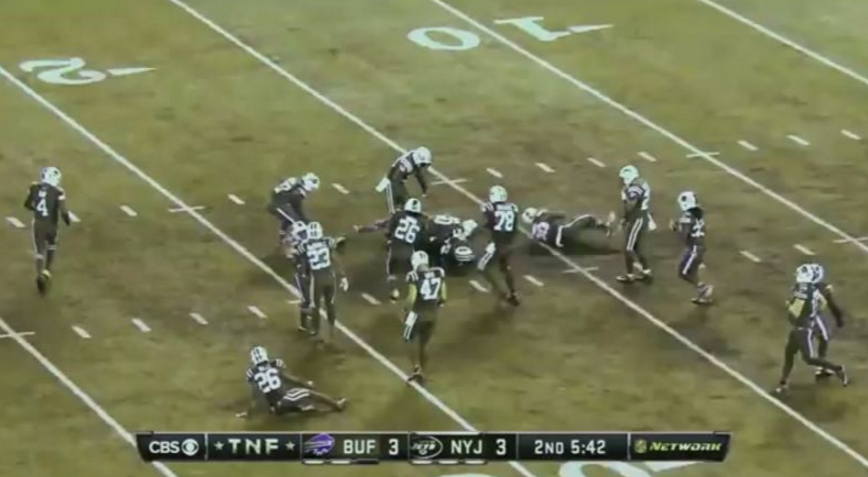
\includegraphics[width=4.5in]{figures/nfl-fig-1.png}
\caption{Jets vs Buffalo}

\end{figure}

\begin{lstlisting}[language=R,caption=.]
\end{lstlisting}

Que una organización tan importante haya caído en un error tan crítico resulta imperdonable pero sirve como ejemplo para recordar que nuestras paletas de colores siempre deben chequearse de forma tal que sean distinguibles para las personas con daltonismo. 

\subsection{Foco en la Funcionalidad}

La funcionalidad de una visualización siempre debe ser la prioridad número uno. Una visualización funcional pero estéticamente desagradable puede arreglarse mediante la aplicación de principios de diseño gráfico. Una visualización estéticamente atractiva pero que no funciona es muy difícil de corregir y a menudo el tiempo invertido en la parte cosmética de la misma se pierde por tener que rediseñar toda la visualización.

\section{Principios de Visualización de Tufte}

Edward Tufte es una de las personas con mayor influencia en el mundo de la visualización de datos siendo el autor de los libros "The Visual Display of Quantitative Information" y "Envisioning Information" los cuales dieron origen al estudio de la visualización de datos como un área importante dentro de Data Science. En esta sección resumimos algunos de los puntos claves de los principios de Tufte sobre visualización de datos.

\subsection{Excelencia}

Sobre la excelencia en la visualización de datos:

\begin{itemize}
\item Consiste en en comunicar ideas complejas con claridad, precisión y eficiencia.
\item Es lo que le da al público la mayor cantidad de ideas en la menor cantidad de tiempo usando la menor cantidad de tinta posible
\item Requiere decir la verdad sobre los datos.
\end{itemize}

Las visualizaciones deben:

\begin{itemize}
\item Mostrar los datos
\item Inducir al público a pensar sobre la sustancia en lugar de la metodología, diseño, tecnología o cualquier otra distracción
\item Evitar distorsionar lo que los datos dicen
\item Presentar mucha información un un espacio reducido
\item Permitir entender sets de datos masivos
\item Estimular el ojo a comparar diferentes datos
\item Revela los datos en diferentes niveles de detalle
\item Servir un propósito claro
\end{itemize}

\subsection{Principios}

Las visualizaciones deben orientarse a los siguientes objetivos:

\begin{itemize}
\item Focalizar en el contenido
\item Comparción en lugar de descripción
\item Integridad
\item Alta resolución
\item Uso de diseños y conceptos clásicos 
\end{itemize}

Foco en el contenido: Por sobre todo lo mas importante es mostrar los datos. El foco debe estar en el contenido de los datos y no en la técnica de visualización empleada. Esto nos lleva a que el diseño debe ser transparente. El éxito de una visualización está basado en el conocimiento de la sustancia que los datos nos transmiten y la calidad, relevancia e integridad del diseño empleado para mostrar esta sustancia.
Hay que asumir que el público es tan inteligente como la persona que crea la visualización. Nunca hay que simplificar una visualización asumiendo que el público no va a entenderla.
\section{Scatter Plots}

Un \textbf{scatter plot} es una de las visualizaciones mas comunes y versátiles, principalmente porque puede adaptarse para diferentes tipos de datos y permite acumular un buen número de dimensiones en un mismo plot. 

En principio en un scatter plot representamos dos variables numéricas en los ejes X e Y y por cada instancia de nuestro set de datos dibujamos un punto en las coordenadas indicadas. 

Estos plots nos dan una idea de la dependencia que existe entre las dos variables y de las características de esta dependencia: lineal, no-lineal, etc.

A un scatter plot básico se le pueden agregar dimensiones controlando el color de los puntos, como en el siguiente ejemplo para el conocido set de datos IRIS.

\begin{figure}[!htb]
\centering
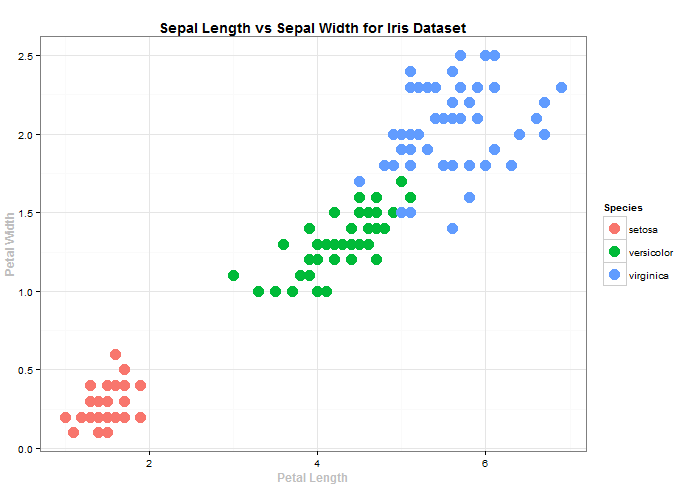
\includegraphics[width=4.5in]{figures/visu-fig-1.png}
\caption{Scatter Plot}

\end{figure}

\begin{lstlisting}[language=R,caption=Scatter Plot Para Iris]
ggplot(data=iris,aes(x=Sepal.Length,y=Sepal.Width,color=Species))+
    geom_point(size=5)+
    xlab("Sepal Length")+
    ylab("Sepal Width")+
    ggtitle("Sepal Length vs Sepal Width for Iris Dataset")
\end{lstlisting}

En el plot vemos la relación entre el largo y ancho de los Pétalos en IRIS mientras que el color muestra la especie recolectada. Claramente hay una fuerte relación lineal positiva entre el largo y ancho de los pétalos. También podemos ver que la especie IRIS setosa tiene pétalos mas pequeños que las otras dos especies y que el tamaño de estos debería ser suficiente para discriminar esta especie de flor de las otras dos. Entre IRIS versicolor e IRIS virginica el tamaño de los pétalos también es un buen discriminador pero hay una cierta superposición que puede generar algunos errores de clasificación si nos basamos únicamente en esta variable.

El color puede representar una variable tanto categórica como numérica en cuyo caso será un gradiente de color. 

Es posible cambiar la forma de los puntos de acuerdo a una variable categórica: círculos, cuadrados, estrellas, triángulos, rombos, etc.

\begin{figure}[!htb]
\centering
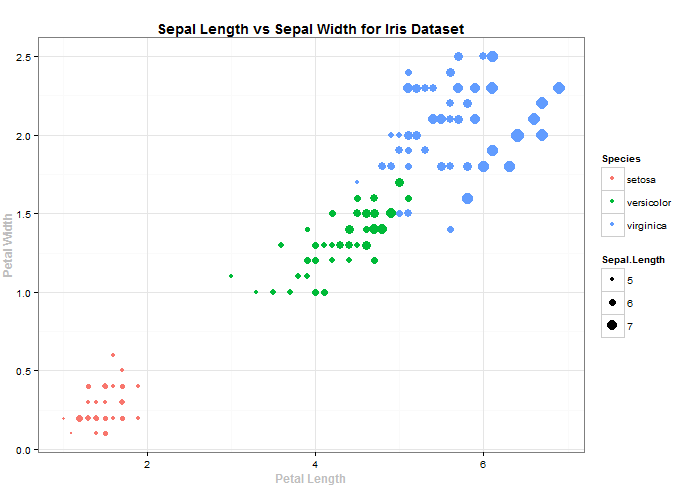
\includegraphics[width=4.5in]{figures/visu-fig-2.png}
\caption{Bubble Plot}

\end{figure}

\begin{lstlisting}[language=R, caption=Bubble plot]
ggplot(data=iris,aes(x=Petal.Length,y=Petal.Width))+
    geom_point(aes(color=Species,size=Sepal.Length))+
    geom_smooth()+
    xlab("Petal Length")+
    ylab("Petal Width")+
    ggtitle("Sepal Length vs Sepal Width for Iris Dataset")
\end{lstlisting}

Si agregamos el tamaño de los puntos para representar una variable numérica tenemos lo que se llama un \textit{bubble plot}. En este caso agregamos el tamaño de los Sépalos para el tamaño de las burbujas. Esto probablemente no aporte mucha claridad al plot pero sirve para ver que Iris Virgínica parece tener sépalos, en general, mas grandes que las otras dos especies de flores. 

Los plots de burbujas se hicieron famosos cuando Hans Rosling mostró su eficacia para transmitir información en una muy famosa charla de TED (The best stats you've ver seen). En esta charla Rosling usó plots de burbujas animados para mostrar la evolución de diferentes países de acuerdo a múltiples dimensiones al mismo tiempo. Por ejemplo usando en el eje $X$ el nivel económico del país (GDP) y en el eje $Y$ la tasa de mortalidad infantil, usando el tamaño de las burbujas para representar la población de los países y el color para indicar su continente. 

El golpe de gracia de la presentación de Rosling fue el uso de la animación para mostrar la evolución del plot de burbujas a lo largo del tiempo. Esto no solo agregó una dimensión extra sino también un importante impacto visual en donde podía, literalmente, verse como los países tendían hacia un mismo equilibrio.

En un Scatter Plot se puede agregar una línea de tendencia que ajuste a la relación entre las variables.

\begin{figure}[!htb]
\centering
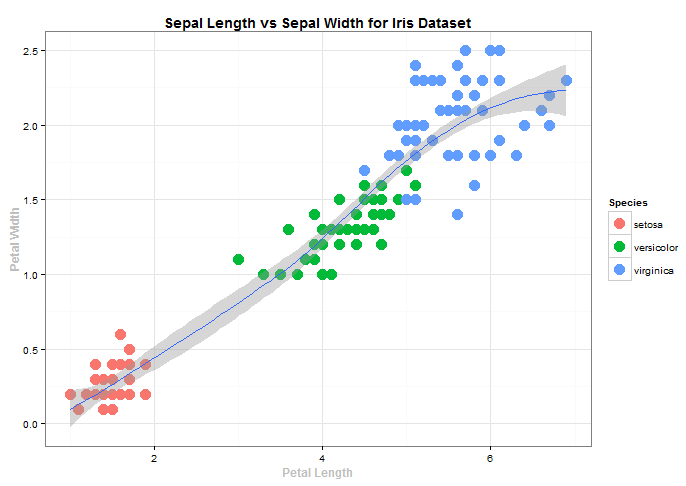
\includegraphics[width=4.5in]{figures/visu-fig-3.png}
\caption{Scatter Plot con Tendencia}

\end{figure}

\begin{lstlisting}[language=R, caption=Scatter Plot con Tendencia]
ggplot(data=iris,aes(x=Petal.Length,y=Petal.Width))+
    geom_point(size=5,aes(color=Species))+
    geom_smooth()+
    xlab("Petal Length")+
    ylab("Petal Width")+
    ggtitle("Sepal Length vs Sepal Width for Iris Dataset")
\end{lstlisting}

La tendencia puede mostrarse de varias formas distintas, desde una simple regresión lineal hasta modelos polinómicos. Es común indicar mediante un área sombreada el grado de confianza que el modelo de tendencia tiene con respecto a los datos. En nuestro plot vemos que la confianza de predecir el ancho de los pétalos en función de su altura decrece para los pétalos mas grandes y es muy efectiva para la especie \textit{iris versicolor} esto lo vemos porque la línea de tendencia es muy angosta al pasar por la zona con los puntos verdes.

Si quisiéramos ver como la tendencia varía según la especie de flor podríamos \textit{facetar} nuestro plot de acuerdo a la especie, esto equivale a hacer un scatter plot por cada especie y luego mostrarlos uno al lado del otro.

\begin{figure}[!htb]
\centering
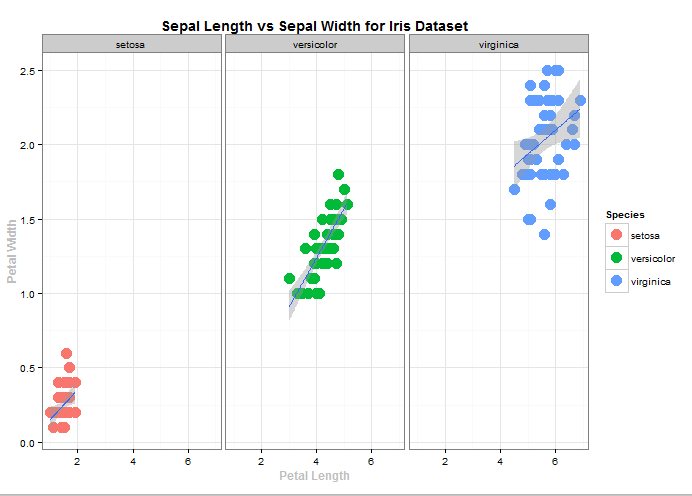
\includegraphics[width=4.5in]{figures/visu-fig-6.png}
\caption{Scatter Plot con Tendencia}

\end{figure}

\begin{lstlisting}[language=R,caption=Scatter Plot Facetado por Especie]
ggplot(data=iris,aes(x=Petal.Length,y=Petal.Width))+
    geom_point(size=5,aes(color=Species))+
    geom_smooth(method="lm")+
    xlab("Petal Length")+
    ylab("Petal Width")+
    ggtitle("Sepal Length vs Sepal Width for Iris Dataset")+
    facet_grid(.~Species)
\end{lstlisting}

Lo que hicimos fue "facetar" nuestro plot de puntos de acuerdo al valor de una variable categórica, en este caso al especie de la flor. Al hacer esto la línea de tendencia es ahora individual para cada plot y podemos observar que es muy efectiva para iris versicolor pero bastante pobre para iris virginica. Es decir que para iris virginica el alto de los pétalos no es tan buen predictor para el ancho de los mismos en comparación con las otras dos especies.

Es posible facetar lado a lado o con un plot debajo de otro. En general esto lo debemos decidir de acuerdo al tamaño de los ejes $X$ e $Y$, cuando $X$ es el eje mas largo es conveniente facetar los plots uno debajo del otro y cuando ocurre lo contrario lado a lado, esto permite minimizar le grado de compresión visual de nuestro plot.

Finalmente veamos un ejemplo en el cual ploteamos el precio de diamantes en función de los carates, está información está disponible en el set de datos "diamonds".

\begin{figure}[!htb]
\centering
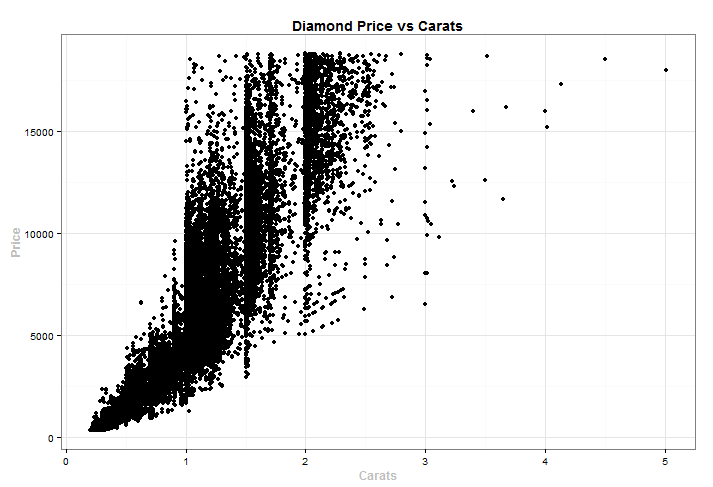
\includegraphics[width=4.5in]{figures/visu-fig-4.png}
\caption{Scatter Plot para Diamonds}

\end{figure}

\begin{lstlisting}[language=R,caption=Scatter Plot con Muchos Puntos]
ggplot(data=diamonds,aes(x=carat,y=price))+
    geom_point(size=2)+
    xlab("Carats")+
    ylab("Price")+
    ggtitle("Diamond Price vs Carats")
\end{lstlisting}

En este plot estamos mostrando un punto para cada par (carats,price) que existe en nuestro set de datos. En principio podemos ver que parece existir una tendencia lineal que indica que cuantos mas carates tiene el diamante mayor es su precio, esto es cierto hasta 1 carate en donde vemos que se produce un efecto muy curioso por el cual aparecen diamantes caros de forma casi independiente de la cantidad de carates de los mismos.

El problema del plot 8.3 es que como tenemos muchos puntos la superposición de los mismos no permite apreciar las zonas en las cuales hay mayor densidad de puntos.  Para solucionar esto podemos usar un valor de transparencia (alpha) para cada punto:

\begin{figure}[!htb]
\centering
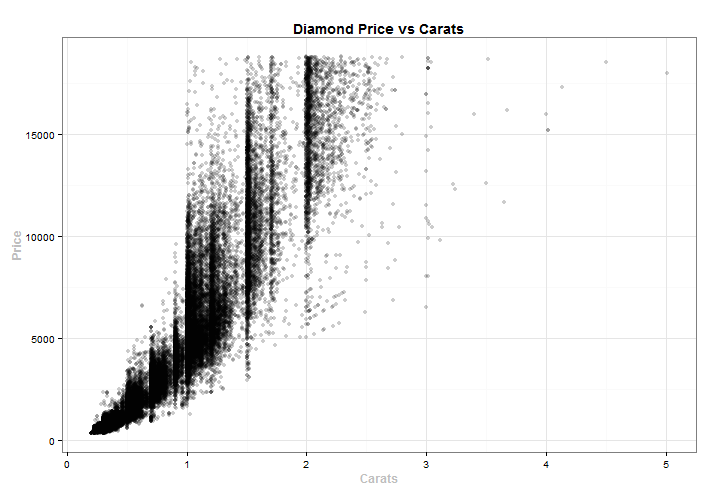
\includegraphics[width=4.5in]{figures/visu-fig-5.png}
\caption{Scatter Plot Para Diamonds con Transparencia}

\end{figure}

\begin{lstlisting}[language=R,caption=Scatter Plot con Transparencia]
ggplot(data=diamonds,aes(x=carat,y=price))+
    geom_point(size=2,alpha=.2)+
    xlab("Carats")+
    ylab("Price")+
    ggtitle("Diamond Price vs Carats")
\end{lstlisting}

Agregando la transparencia podemos ver como mejor nitidez las zonas en las que se concentran la mayoría de los diamants, vemos que hay muchos diamantes de 1, 1.5 o 2 carates y que los diamantes de mas de 2 carates son raros y de mas de 3 carates muy raros. Si cortamos verticalmente el gráfico por debajo del precio de 5000 dólares es muy difícil apreciar tendencia alguna, es decir que aprendemos que podemos usar carates para predecir el precio solo para diamantes de menos de un carate, luego de esto hay otros factores que seguramente son mas importantes.

Veamos que sucede si hacemos un scatter plot en donde el eje $x$ es una variable categórica:

\begin{figure}[!htb]
\centering
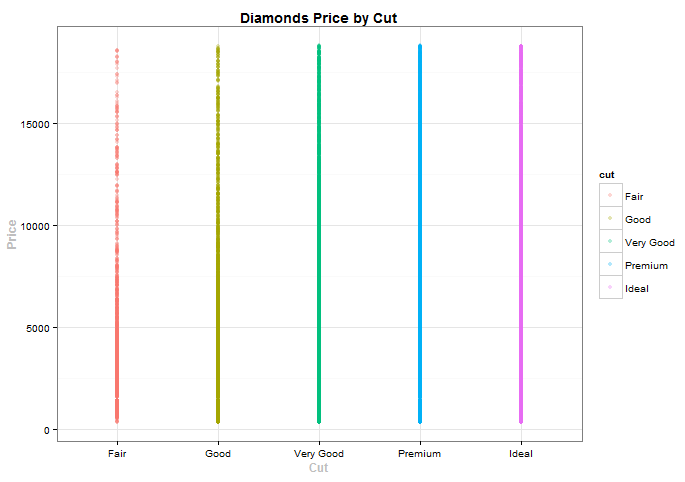
\includegraphics[width=4.5in]{figures/visu-fig-12.png}
\caption{Scatter Plot Para Una Variable Categórica (MAL)}

\end{figure}

\begin{lstlisting}[language=R,caption=Scatter Plot para Variables Categóricas (MAL)]
ggplot(diamonds, aes(x=cut, y=price,color=cut)) +
    geom_point(alpha=0.3) +
    xlab("Cut") +
    ylab("Price")+
    ggtitle("Diamonds Price by Cut") +
\end{lstlisting}

Este plot no funciona bien ya que en el eje x nuestros puntos solo pueden tomar 5 valores posibles por lo tanto solo tenemos unas líneas finitas que no tienen mucho sentido. Existe una forma de que este plot funcione que consiste en perturbar un poco cada punto, de esta forma no todos tendrán el mismo valor en $x$, a este proceso se lo denomina \textit{jittering} y el resultado es el siguiente:

\begin{figure}[!htb]
\centering
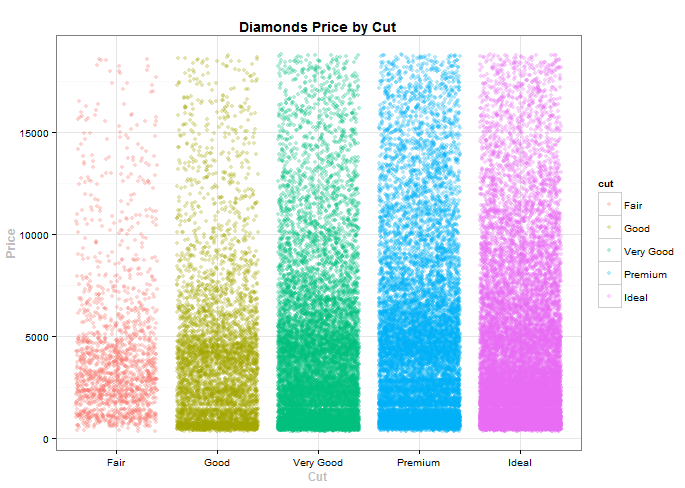
\includegraphics[width=4.5in]{figures/visu-fig-13.png}
\caption{Scatter Plot Para Una Variable Categórica Usando Jittering}

\end{figure}

\begin{lstlisting}[language=R,caption=Scatter Plot para Variables Categóricas con Jittering]
ggplot(diamonds, aes(x=cut, y=price,color=cut)) +
    geom_jitter(alpha=0.3) +
    xlab("Cut") +
    ylab("Price")+
    ggtitle("Diamonds Price by Cut") 
\end{lstlisting}

En este plot vemos mucho mejor la forma en que se distribuyen los diamantes de acuerdo a su corte y precio. Es curioso que independientemente del corte existan gran cantidad de diamantes con un precio elevado aunque está claro que esto es recién visible a partir de "very good", vemos que la zona de máxima densidad en el precio aumenta al pasar de "fair" a "good" pero es mas difícil distinguir el efecto, si existiera al pasar de "very good" a "premium" o "ideal".

Resumimos ahora las características generales de un Scatter Plot que es un plot muy versátil y que permite mostrar información usando varias dimensiones al mismo tiempo.

\begin{enumerate}
\item Los ejes x e y deben ser variables numéricas
\item Puede usarse el color para agregar una variable categórica o numérica
\item Puede usarse el tamaño de los puntos para agregar una variable categórica o numérica
\item Puede usarse transparencia para darle mayor claridad al plot
\item Puede agregarse una función de tendencia
\item Puede usarse la forma de los puntos para agregar una variable categórica.
\end{enumerate}

\section{Gráficos de Barras}

Los gráficos de barras son muy populares, y constituyen una de las visualizaciones en donde mayor cantidad de errores se cometen. Hay dos principios básicos a observar cuando hacemos gráficos de barras: una de las variables tiene que ser categórica y los ejes deben comenzar en cero. La variable categórica es aquella para la cual vamos a crear las barras, una barra por cada valor posible de la variable.

Empecemos con un ejemplo muy simple usando el set de datos mtcars que tiene información sobre autos, creemos un gráfico de barras con la cantidad de autos  que hay para las diferentes cantidades de cilindros posibles.

\begin{figure}[!htb]
\centering
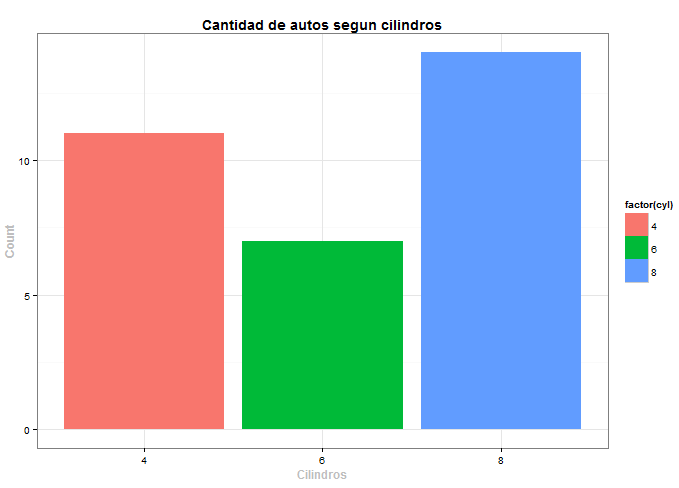
\includegraphics[width=4.5in]{figures/visu-fig-7.png}
\caption{Plot de Barras para MtCars}

\end{figure}

\begin{lstlisting}[language=R,caption=Gráfico de Barras simple]
ggplot(mtcars, aes(factor(cyl))) +
    geom_bar(aes(fill=factor(cyl))) +
    xlab("Cilindros")+
    ylab("Count")+
    ggtitle("Cantidad de autos segun cilindros")
\end{lstlisting}

Hemos usado el color simplemente para reforzar el concepto de que cada barra corresponde a una categoría diferente, no es algo necesario y es redundante con el eje $x$ del plot pero mejora la visualización. Como podemos ver hay mas autos de 8 cilindros que 6 y 4 y los de 4 son mas populares que los de 6.

Por supuesto es posible dividir cada barra en zonas según una variable categórica,  por ejemplo el tipo de corte de diamante para observar de que forma se compone la cantidad de cada uno de los diferentes niveles de claridad de los diamantes. 

\begin{figure}[!htb]
\centering
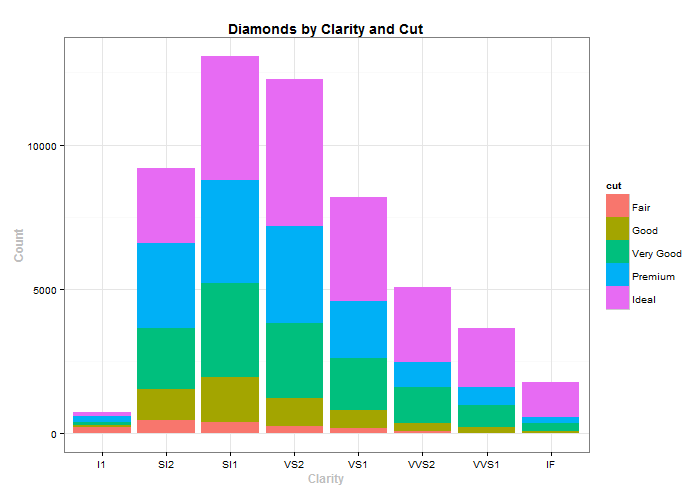
\includegraphics[width=4.5in]{figures/visu-fig-8.png}
\caption{Plot de Barras Apiladas}

\end{figure}

\begin{lstlisting}[language=R,caption=Plot de Barras Apiladas]
ggplot(diamonds, aes(clarity, fill=cut)) +
    geom_bar() +
    xlab("Clarity") +
    ylab("Count")+
    ggtitle("Diamonds by Clarity and Cut") 
\end{lstlisting}

En un gráfico con barras apiladas la altura de cada barra es el total para la categoría indicada en el eje $X$ y cada barra se sub-divide en alturas proporcionales de acuerdo a otra variable categórica que en nuestro caso es el corte del diamante. 

Podemos ver por ejemplo que para todos los niveles de claridad existe una buena cantidad de diamantes con corte "premium" y en general parece ser que el tipo de corte no depende de la claridad excepto para "frair" y "good" en donde notamos que a medida que aumenta la claridad la cantidad de diamantes correspondientes a esos cortes disminuye.

Una variante es forzar a que todas las barras ocupen la misma altura, esto lo podemos hacer creando una variable adicional que indique que porcentaje del total de cada valor de la variable categórica toma la otra variable. 

\begin{figure}[!htb]
\centering
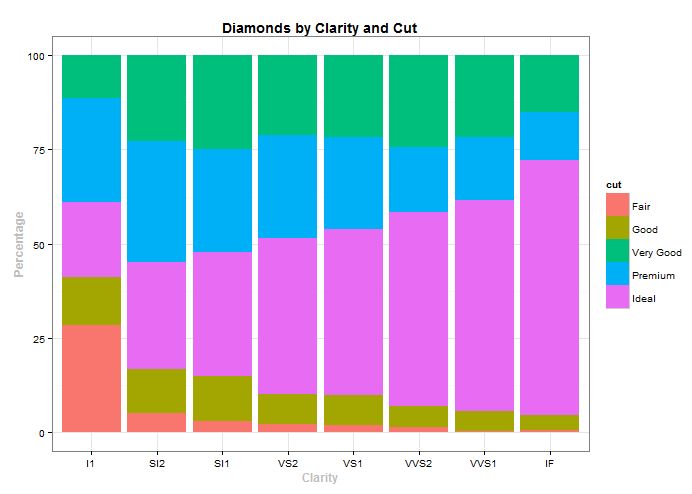
\includegraphics[width=4.5in]{figures/visu-fig-9.png}
\caption{Plot de Barras Apiladas Completas}

\end{figure}

\begin{lstlisting}[language=R,caption=Plot de Barras Apiladas completas]
ggplot(diamonds, aes(clarity,fill=cut)) +
    geom_bar(position="fill") +
    xlab("Clarity") +
    ylab("Count")+
    ggtitle("Diamonds by Clarity and Cut") 
\end{lstlisting}

Podemos ver que ahora el eje $Y$ va de 0 a 100 indicando un porcentaje, en este plot ya no tenemos información sobre el total de diamantes por cada nivel de claridad pero es mas simple comparar la cantidad de diamantes de cada corte según el nivel de claridad. Es decir que perdemos información pero ganamos claridad en otro aspecto. Aquí podemos ver muy claramente que a medida que aumenta la claridad la cantidad de diamantes con corte "fair" o "good" disminuye. Esto no ocurre con los cortes que son "very good" o superior.

Otra variante es mostrar las barras una al lado de la otra en lugar de apiladas:

\begin{figure}[!htb]
\centering
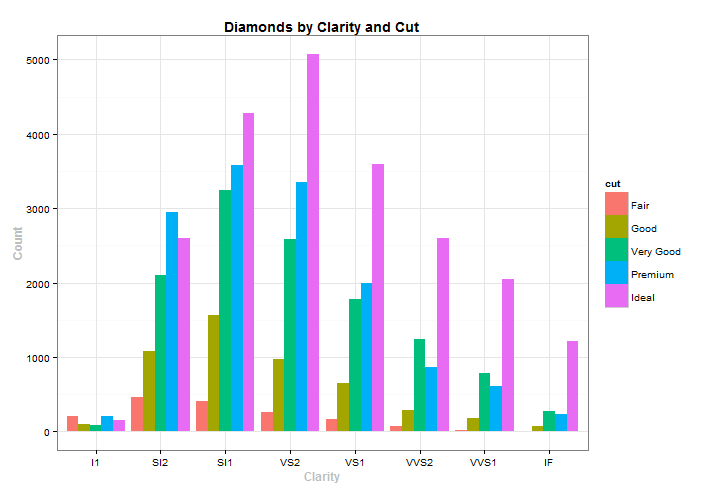
\includegraphics[width=4.5in]{figures/visu-fig-10.png}
\caption{Plot de Barras Contiguas}

\end{figure}

\begin{lstlisting}[language=R,caption=Plot de Barras Contiguas]
ggplot(diamonds, aes(clarity, fill=cut)) +
    geom_bar(position="dodge") +
    xlab("Clarity") +
    ylab("Count")+
    ggtitle("Diamonds by Clarity and Cut") 
\end{lstlisting}

En esta variante el plot podemos ver la cantidad de diamantes para cada combinación de claridad y corte. Por cada nivel de claridad tenemos tantas barras como cortes existen. Aquí vemos claramente que para la claridad V82 en adelante el corte "ideal" empieza a ser predominante, esto quiere decir que para diamantes con gran claridad no se hacen trabajos de corte económicos sino que se busca la perfección. Para diamantes con niveles de claridad pobres la distribución de los cortes es mas pareja, es decir que puede haber tantos cortes "fair" como "ideal" en cantidades similares para un diamante con el nivel de claridad mas bajo posible.

Hay que tener cuidado con la cantidad de barras dentro de cada "columna" de nuestro plot, si son muchas la interpretación del mismo puede volverse dificultosa. Observemos como este tipo de plot es en realidad un plot de barras en donde cada barra es otro plot de barras.

Es común en ciertos medios manipular la percepción de la audiencia cambiando la escala de los ejes de un gráfico de barras. Cuando los ejes no comienzan en cero un plot de barras puede mostrar una diferencia sustancial en el valor de dos variables cuando en realidad en la versión completa (y correcta) del plot se verían muy parecidas.

\section{Histogramas y Plots de Densidad}

Un histograma sirve para mostrar la distribución de una determinada variable, es decir la cantidad de veces que la variable toma determinados valores. Para construir un histograma hacen falta dos parámetros: la variable en cuestión que tiene que ser numérica (continua o discreta) y el ancho que van a tener las columnas del histograma. Por ejemplo si una variable puede tomar valores continuos entre 0 y 10 y queremos que nuestro histograma tenga 20 columnas entonces el ancho de las mismas será de 0.5. Nuestro histograma tendrá entonces la cantidad de veces que la variable toma valor entre 0 y 0.5, luego entre 0.5 y 1.0, etc.

Es importante destacar que un histograma, si bien muestra barras, es completamente diferente a un plot de barras. En el histograma la variable $x$ es numérica mientras que en el plot de barras es categórica, en un histograma el eje $x$ siempre está ordenado mientras que en un plot de barras puede tener cualquier orden. En un histograma no puede haber espacios entre las barras y en un plot de barras si, el eje $y$ en un plot de barras puede ser cualquier valor numérico mientras que en un histograma siempre es una cantidad.

Nuestro primer histograma muestra la distribución de la variable carats en el set de datos diamonds.

\begin{figure}[!htb]
\centering
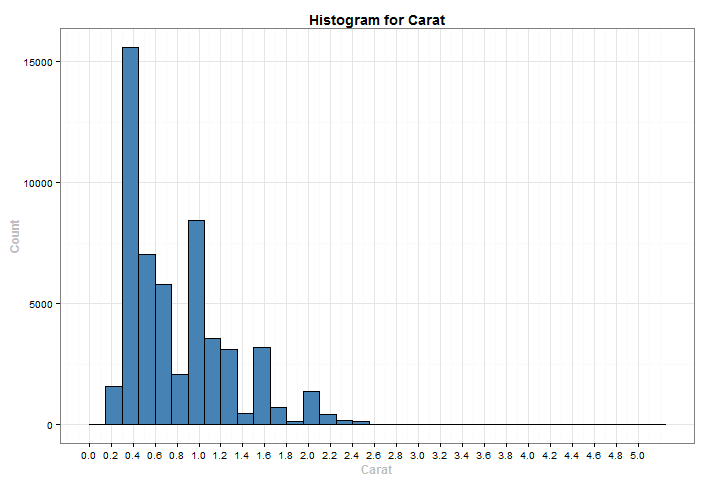
\includegraphics[width=4.5in]{figures/visu-fig-14.png}
\caption{Histograma para Carats}

\end{figure}

\begin{lstlisting}[language=R,caption=Histograma para Carats]
ggplot(diamonds,aes(x=carat)) +
    geom_histogram(color="black",fill="steelblue",binwidth=.15) +
    xlab("Carat") +
    ylab("Count") +
    scale_x_continuous(breaks=seq(0,5,.2))+
    ggtitle("Histogram for Carat") 
\end{lstlisting}

El histograma nos muestra la distribución de la variable "carats" el eje $X$ miuestra los posibles valores de la variable discretizados de acuerdo a ciertos intervalos y el eje $Y$ indica la cantidad de veces que la variable cayó dentro de cada uno de esos intervalos para nuestro set de datos. En el caso de carats vemos que los valores menores a 1.5 son los mas populares pero hay algunos diamantes que pueden llegar hasta 5, esta es una distribución \textit{right skewed} porque presenta una cola larga hacia la derecha.

El color del histograma es simplemente decorativo y no debería nunca tener colores diferentes para cada barra. Si cambiamos el parámetro \textit{binwidth} podemos crear un histograma con mas o menos granularidad.

\begin{figure}[!htb]
\centering
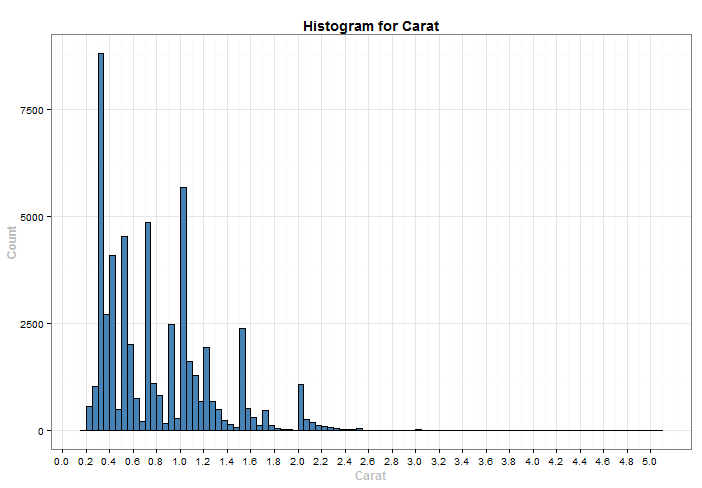
\includegraphics[width=4.5in]{figures/visu-fig-15.png}
\caption{Histograma para Carats con mas bins}

\end{figure}

\begin{lstlisting}[language=R,caption=Histograma para Carats con mas bins]
ggplot(diamonds,aes(x=carat)) +
    geom_histogram(color="black",fill="steelblue",binwidth=.05) +
    xlab("Carat") +
    ylab("Count") +
    scale_x_continuous(breaks=seq(0,5,.2))+
    ggtitle("Histogram for Carat") 
\end{lstlisting}

En la segunda versión discretizamos carats en una mayor cantidad de intervalos (bins) en donde antes teníamos una sola barra ahora tenemos varias mostrando valores mas precisos de la variable, en general no es necesario tener una gran cantidad de bins ya que con unos 10 a 20 bins suele alcanzar para entender la distribución de la variable. El tamaño de cada bin puede calcularse como $(max-min)/k$ siendo $k$ la cantidad de bins que queremos mostrar en el histograma.

Un plot de densidad es una versión continua de un histograma, aquí no hace falta indicar el tamaño de los bins. Lo que se muestra es como se distribuye la densidad de la variable numérica a lo largo de todos sus valores posibles.

\begin{figure}[!htb]
\centering
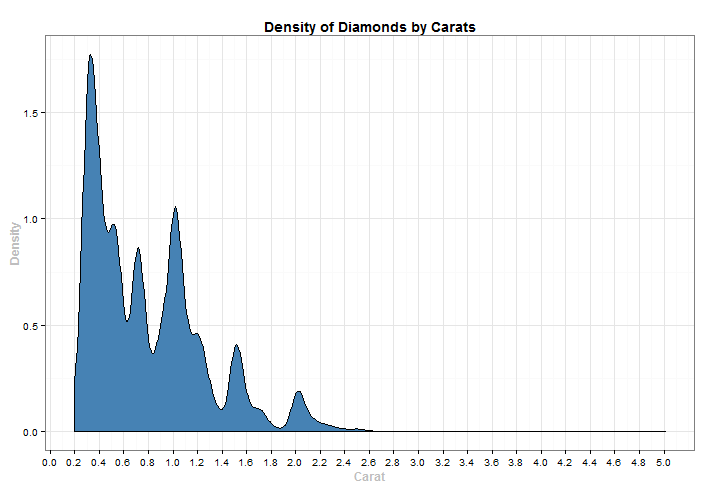
\includegraphics[width=4.5in]{figures/visu-fig-16.png}
\caption{Plot de Densidad para Carats}

\end{figure}

\begin{lstlisting}[language=R,caption=Plot de Densidad para Carats]
ggplot(diamonds,aes(x=carat)) +
    geom_density(fill="steelblue") +
    xlab("Carat") +
    ylab("Density") +
    scale_x_continuous(breaks=seq(0,5,.2))+
    ggtitle("Density of Diamonds by Carats") 
\end{lstlisting}

Aquí es mas evidente el efecto del \textit{long tail} hacia la derecha, debemos destacar que si el eje $X$ llega hasta el valor 5.0 es porque en algún momento la variable carats toma este valor, sin dudas un diamante muy valioso. 

Este histograma nos muestra picos entorno a los valores de carats 0.5,1.0  y 1.5 probablemente porque se trata de valores populares por el redondeo. Cuando tenemos estos múltiples picos en un plot de densidad siempre tenemos que considerar cuál es el motivo por el cual los datos presentan picos para ciertos valores en lugar de distribuirse de forma continua. En general la explicación es que la variable no es realmente continua sino que es semi-continua, es decir que tiene una cierta cantidad de valores que toma con mas frecuencia que otros, esto es equivalente, en cierta forma, a una discretización natural de la variable.

Podemos superponer varios plots de densidades o histogramas usando una variable categórica como separador.

\begin{figure}[!htb]
\centering
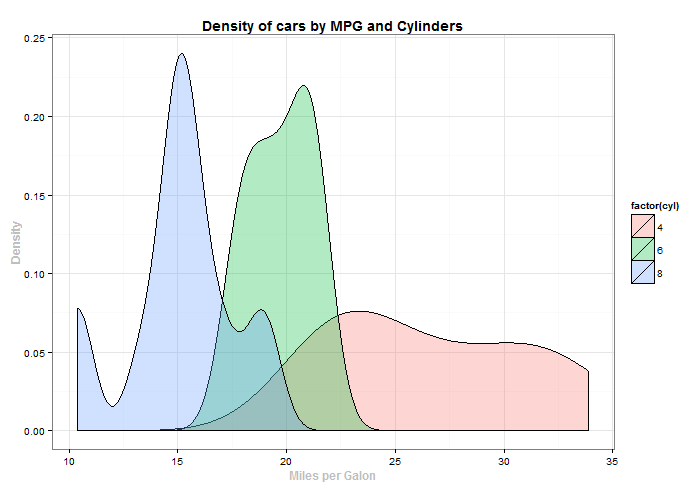
\includegraphics[width=4.5in]{figures/visu-fig-18.png}
\caption{Plot de Densidad para MPG por cilindros en Mtcars }

\end{figure}

\begin{lstlisting}[language=R,caption=Plot de Densidad para MPG por cilindros en MtCars]
ggplot(mtcars,aes(x=mpg,fill=factor(cyl))) +
    geom_density(alpha=0.3) +
    xlab("Miles per Galon") +
    ylab("Density") +
    ggtitle("Density of cars by MPG and Cylinders") 
\end{lstlisting}

Aquí vemos que cantidad de autos tenemos en mtcars según los distintos valores que puede tomar la variable "mpg" (consumo) de acuerdo a la cantidad de cilindros del auto. Observamos que a mayor cantidad de cilindos mayor es el consumo. 

Vemos también la distribución prácticamente normal de los autos de 6 cilindros y una distribución semi-uniforme para los de 4 cilindros, los autos de 8 cilindros presentan una extraña distribución que parece ser bimodal o trimodal (tiene dos o tres picos según como la interpretemos). 

\section{Boxplots}

Un \textit{boxplot} es una forma de visualizar la distribución de una variable numérica, en general se usa para comparar la distribución de la variable de acuerdo a una variable categórica mostrando varios boxplots uno al lado del otro en el eje x. 

Veamos un ejemplo rápido de un boxplot para MtCars.

\begin{figure}[!htb]
\centering
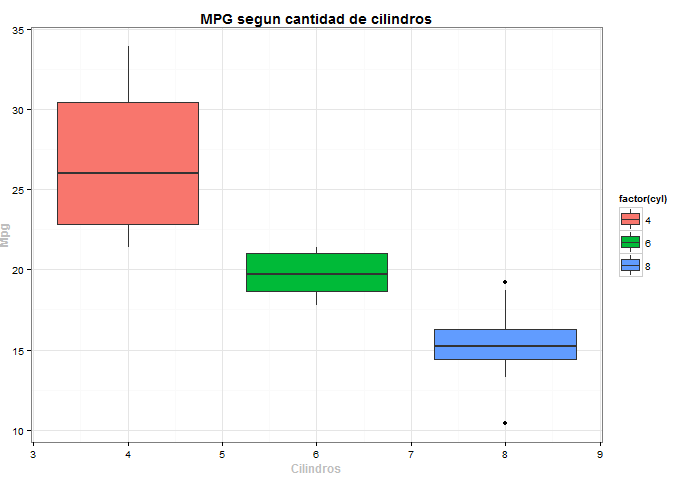
\includegraphics[width=4.5in]{figures/visu-fig-19.png}
\caption{Boxplot para mpg según cantidad de cilindros }

\end{figure}

\begin{lstlisting}[language=R,caption=Boxplot para mpg según cantidad de cilindros]
ggplot(mtcars,aes(x=cyl,y=mpg,fill=factor(cyl))) +
    geom_boxplot()+
    xlab("Cilindros") +
    ylab("Mpg") +
    ggtitle("MPG segun cantidad de cilindros") 
\end{lstlisting}

El color en este caso no es necesario ya que el eje $X$ indica la cantidad de cilindros, esto sigue los principios básicos que listamos al comenzar el capítulo ya que en blanco y negro la interpretación del plot sería la misma. El eje $Y$ nos da una idea de los valores que puede tomar la variable mpg en nuestro set de datos. 

El plot nos muestra que el rendimiento (mpg) es mayor para los autos de 4 cilindros, también podemos ver que los autos de 4 cilindros tienen una distribución mas "amplia" ya que el tamaño de su boxplot es mayor. Expliquemos cuáles son los elementos en un boxplot para volver a analizar nuestro plot.

\begin{figure}[!htb]
\centering
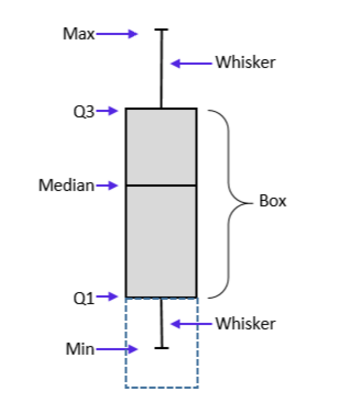
\includegraphics[width=2.5in]{figures/boxplot-fig-1.png}
\caption{Elementos de un Boxplot}

\end{figure}

\begin{lstlisting}[language=R,caption=Elementos de un boxplot]
\end{lstlisting}

La "caja" del boxplot va desde el primer al tercer cuantil, es decir que el 25\% de los datos están por debajo de la caja y el 25\% de los datos están por encima de la caja. La caja concentra entonces el 50\% de los datos y la línea dentro de la caja muestra la media. Las líneas que salen de la caja van desde el primer cuantil hasta el valor mínimo y máximo, los puntos son valores anómalos (outliers).

Regresando al boxplot que hicimos vemos que para 4 cilindros vemos que hay mas autos desde la mediana al tercer cuantil que desde la mediana al primer cuantil es decir que hay menor variabilidad en el consumo por debajo de la mediana que por encima.Esto indica una variable con un leve left skew.  Para los autos de 8 cilindros vemos que hay valores anómalos, hay un auto que tiene un consumo excesivo y otro que tiene un consumo muy bueno para ser un auto de 8 cilindros. Vemos también que para los autos de 6 cilindros la distribución es muy pareja, prácticamente normal. 

\begin{figure}[!htb]
\centering
\includegraphics[width=5.5in]{figures/visu-fig-20.png}
\caption{Boxplot y Plot de Densidad}

\end{figure}

\begin{lstlisting}[language=R,caption=Boxplot y plot de densidad]
\end{lstlisting}

La comparación entre el boxplot y el plot de densidad nos muestra que ambos plots contienen prácticamente la misma información, observemos el "pico" de la distribución para 8 cilindros que en el boxplot aparece como un outlier.

 Para 6 cilindros la distribución es prácticamente normal y eso también se ve en el boxplot, también vemos que tiene poca variabilidad porque hay muy poca distancia entre el mínimo y el máximo. Para 4 cilindros el boxplot nos dice que la distribución es mas "ancha" y que está volcada hacia la izquierda cosa que vemos en el plot de densidad. 

Un boxplot puede mostrar si una variable presenta skewing pero no puede indicar la modalidad de la misma. En el boxplot para 8 cilindros no podemos darnos cuenta que se trata de una variable trimodal. 

La ventaja de un boxplot es que podemos plotear una gran cantidad de boxplots uno al lado del otro para comparar de acuerdo a una variable categórica con muchos valores caso en el cual un plot de densidad, incluso usando transparencia, sería bastante confuso. Este es un recurso muy útil para entender si una variable afecta la distribución de otra. 

Veamos para "clarity" en diamonds como se distribuye el precio.

\begin{figure}[!htb]
\centering
\includegraphics[width=4.5in]{figures/visu-fig-21.png}
\caption{Boxplot para Clarity vs Price}

\end{figure}

\begin{lstlisting}[language=R,caption=Boxplot para Clarity vs Price]
ggplot(diamonds,aes(x=clarity,y=price,fill=factor(clarity))) +
    geom_boxplot()+
    xlab("Clarity") +
    ylab("Price") +
    ggtitle("Price by Clarity for Diamonds")
\end{lstlisting}

El boxplot nos da al mismo tiempo información de como se distribuye el precio de los diamantes para todos los valores posibles de "clarity". Como podemos ver hay muchos outliers en todos los casos y siempre hacia arriba, es decir que independientemente de su "claridad" es posible que un diamante tome un valor muy alto. Los precios inusualmente bajos son en cambio prácticamente nulos, es decir que no hay diamantes muy baratos cosa que podríamos llegar a sospechar. 

Vemos que la distribución en algunos lados es muy despareja, la presencia de los outliers hace que en todos los casos tengamos un fuerte "right skew" la mayoría de los valores son precios bajos pero hay un "long tail" de precios muy altos, es decir diamantes muy valiosos. 

La mediana nos indica que el valor medio de un diamante no depende de su claridad, el valor medio mas alto está dado para un nivel de claridad bajo (SI2) y se debe probablemente a la gran cantidad de outliers que presenta esta categoría. Los niveles de claridad mas altos muestran cajas de menor altura, mas compactas lo cual denota distribuciones con menor variabilidad. 

Para clarificar la situación es muchas veces una buena idea acompañar un boxplot de un plot de densidad o incluso de un scatter plot usando jittering. Estos plots al ser standard se pueden generar rápidamente para el análisis exploratorio de datos.

\begin{figure}[!htb]
\centering
\includegraphics[width=4.5in]{figures/visu-fig-22.png}
\caption{Violin Plot}

\end{figure}

\begin{lstlisting}[language=R,caption=Scatter plot para Price vs Clarity]
ggplot(data=diamonds,aes(x=clarity,y=price,color=clarity))+
    geom_jitter(size=2,alpha=.2)+
    xlab("Clarity")+
    ylab("Price")+
    ggtitle("Diamond Price vs Clarity")
\end{lstlisting}

En el scatter plot (usando jittering) vemos la confirmación de lo que se deduce en el boxplot, para todas las claridades la mayoría de los diamantes tiene u precio bajo pero con varios valores altos. 

Vemos también que el efecto es menor en "I1" que en el boxplot vemos que tiene menos outliers. El caso de la claridad "IF" en donde el boxplot nos mostró menor variabilidad queda ahora mas claro, hay menos cantidad de diamantes "IF" y la mayoría de ellos tiene un precio bajo. Es curioso e interesante ver que para todas las claridades excepto I1 hay una zona de precios bajos con una cantidad importante de diamantes. Como curiosidad vemos también una cierta separación en el rango de precios entre los diamantes que están en el rango mas bajo y todos los demás, esto podría deberse a la existencia de algún tipo de convención de precios para los diamantes mas económicos. 

Todas estas hipótesis que surgen de estos plots son parte del resultado del análisis exploratorio de los datos, luego en caso de que nos resulte conveniente podemos aplicar algoritmos para verificar estas hipótesis.

En algunos casos cuando los outliers son muchos el boxplot puede no permitir comparar claramente cuál de las variables tiene mas o menos outliers, existe una variante del boxplot que soluciona esto denominada \textit{plot de violín}

\begin{figure}[!htb]
\centering
\includegraphics[width=4.5in]{figures/visu-fig-23.png}
\caption{Violin Plot}

\end{figure}

\begin{lstlisting}[language=R,caption=Violin plot para Price vs Clarity]
ggplot(diamonds,aes(x=clarity,y=price,fill=factor(clarity))) +
    geom_violin()+
    xlab("Clarity") +
    ylab("Price") +
    ggtitle("Price by Clarity for Diamonds") +
    my_theme
\end{lstlisting}

El plot de violín nos muestra un ancho correspondiente a la densidad de la variable para el valor del eje $Y$ correspondiente. Es mucho mas sencillo interpretar el histograma de la variable en base al plot de violín en todos los casos tendremos "right skewing" pero en el caso de las claridades a la derecha la desproporción es mucho mayor. Vemos también que para "I1" la cantidad de valores anómalos es menor que para los otros valores de clarity.

En el plot de violín el ancho es un elemento visual importante a diferencia de un boxplot tradicional. El color tampoco es importante, el mismo plot de violín en blanco y negro sería efectivo. El rango de los ejes es igual al boxplot. 

En general puede ser buena idea realizar tanto el boxplot como el plot de violín, estos plots junto un plot de densidad por cada categoría nos ayudarán a entender perfectamente las características estadísticas de una variable.

Es posible agregar una variable categórica con pocos valores posibles extra en un boxplot cuando los resultados no se tornan confusos, en este caso usando el color para distinguir entre dos variables posibles: caja automática o manual.

\begin{figure}[!htb]
\centering
\includegraphics[width=4.5in]{figures/visu-fig-24.png}
\caption{Boxplot según una segunda variable categórica}

\end{figure}

\begin{lstlisting}[language=R,caption=Boxplot con una segunda variable categórica]
ggplot(mtcars, aes(factor(cyl), mpg)) + 
    geom_boxplot(aes(fill=factor(am))) +
    xlab("Cilindros") +
    ylab("Mpg") +
    ggtitle("MPG segun cantidad de cilindros (automaticos vs manuales)")
\end{lstlisting}

En el plot vemos en rojo los autos automáticos y en azul los manuales, vemos que para 4 cilindros los autos manuales tienen mejor rendimiento (menor consumo), esta tendencia se verifica también para 6 cilindros. Para 8 cilindros la tendencia desaparece y es aparentemente igual tener un auto manual o automático si nos preocupa el consumo, esto tal vez se deba a que un motor de gran cilindrada consume tanto que el efecto del tipo de transmisión es despreciable.

\section{Gráficos de Líneas}

Los gráficos de líneas son muy útiles, pero tienen una muy fuerte limitación, en casi todos los casos el eje $X$ debe ser tiempo. Por lo tanto es un plot dedicado casi exclusivamente a series temporales. La variable en el eje $Y$ puede ser de cualquier tipo aunque casi siempre es ordinal, ya sea numérica (el caso mas frecuente) o categórica. El eje $X$ representa entonces la evolución del valor de dicha variable a lo largo del tiempo.

Veamos un ejemplo para el precio de la acción IBM a lo largo del tiempo:

\begin{figure}[!htb]
\centering
\includegraphics[width=4.5in]{figures/visu-fig-25.png}
\caption{Plot de líneas para las acciones de IBM}

\end{figure}

\begin{lstlisting}[language=R,caption=Plot de líneas para las acciones de IBM]
ggplot(ibm,aes(Date,Close)) + 
    geom_line(size=1.1,color="steelblue") +
    xlab("Date")+
    ylab("Stock Price")+
    ggtitle("Stock Market")+
    scale_x_date(labels = date_format("\%b-\%y"),breaks = date_breaks("6 months"))
\end{lstlisting}

Vemos que la tendencia de IBM fue alcista hasta aproximadamente mayo de 2013 y luego inició un descenso, dentro de esta tendencia la variable tiene zonas donde crece y zonas donde decrece, esto es muy común en el mercado de valores y en general en muchas variables económicas donde el crecimiento de una variable se explica mediante el efecto acumulativo de varias alzas y bajas. 

Cuando nuestro set de datos tiene el formato (date,name,value) y name es una variable categórica podemos usar la misma para plotear varias líneas al mismo tiempo usando diferentes colores.

\begin{figure}[!htb]
\centering
\includegraphics[width=4.5in]{figures/visu-fig-26.png}
\caption{Plot de líneas para varias acciones}

\end{figure}

\begin{lstlisting}[language=R,caption=Plot de líneas para varias acciones]
ggplot(stock,aes(Date,Close,color=stock)) + 
    geom_line(size=1.1) +
    xlab("Date")+
    ylab("Stock Price")+
    ggtitle("Stock Market")+
    scale_x_date(labels = date_format("\%b-\%y"),breaks = date_breaks("6 months"))
\end{lstlisting}

El plot compara las acciones de IBM, Apple y Linkedin durante 5 años, notemos que el plot de IBM tiene la misma forma pero ha cambiado en función de la escala porque APPLE tenía un valor para su acción mucho mas alto hasta que se desplomo en Junio de 2014. Podemos ver que la tendencia de Apple muestra en principio una cierta recuperación que vuelve a caer, IBM es la acción con valor mas estable y Linkedin tiene un comportamiento bastante variable.

Una opción interesante es usar el eje $Y$ para representar el ranking de una variable en un cierto instante de tiempo. Por ejemplo:

\begin{figure}[!htb]
\centering
\includegraphics[width=4.5in]{figures/visu-rank-fig-1.png}

\caption{Gráficos de Líneas usando el eje $Y$ para mostrar Ranking}
\label{fig:lineasranking}
\end{figure}

La figura ~\ref{fig:lineasranking} nos muestra un gráfico de líneas para la popularidad de lenguajes en StackOverflow, en donde el eje $Y$ representa el ranking del lenguaje a lo largo del tiempo. Este tipo de gráficos son mucho mas legibles que la alternativa de representar la cantidad de preguntas o tags de cada lenguaje a lo largo del tiempo.

Al usar el ranking en el eje $Y$ se pierde la escala entre los valores de las diferentes categorías. Por ejemplo si la diferencia entre el primero y el segundo es mucho mayor que la diferencia entre el segundo y el tercero en este tipo de plots no se podría apreciar dicha diferencia.

Este tipo de plots pueden quedar muy bien en versiones interactivas en las que el usuario pueda seleccionar algunas de las variables a mostrar y que estas aparezcan en colores en el plot dejando a las otras en un tono de background, similar a lo que vemos en la figura ~\ref{fig:lineasranking}

En todos los casos el gráfico se lee de izquierda a derecha y los valores de interés deben leerse en el eje $Y$, cuando alguna de las variables está muy fuera de escala en relación a las demás se produce un efecto de compresión visual que puede dificultar la visualización del plot. En nuestro caso APPLE domina los valores del eje $T$ lo cual hace que el plot de IBM parezca mucho mas plano de lo que es realmente como vimos en el plot anterior. 

Los plots de líneas son extremadamente sensibles a valores erróneos o fuera de escala, basta que en algún momento alguna de las variables en el plot tome un valor inusualmente alto para que todo el plot quede comprimido a algo que no tiene sentido visual alguno. 

\section{Gráficos de área}

Una variante de los gráficos de línea son los gráficos de área en donde el eje $X$ sigue siendo el tiempo y el eje $Y$ sigue siendo una variable pero ahora mostramos el área debajo de cada curva de forma proporcional al valor de la misma. Esto NO es lo mismo que colorear el área debajo de las curvas ya que el área debe ser proporcional al valor de la variable según alguna variable categórica.

Veamos como ejemplo un plot de área para la cantidad de películas por categoría a lo largo del tiempo.

\begin{figure}[!htb]
\centering
\includegraphics[width=4.5in]{figures/visu-fig-27.png}
\caption{Plot de áreas para películas}

\end{figure}

\begin{lstlisting}[language=R,caption=Plot de áreas para películas]
ggplot(mtypes,aes(x=year,y=total,fill=category))+
    geom_area()+
    xlab("Year")+
    ylab("Number of Movies")+
    ggtitle("Movie Categories Across Time")
\end{lstlisting}

En el plot podemos ver que las categorías mas populares son "drama" y "comedia", las películas de acción se vuelven mas populares luego de los 80. Podemos ver también el auge de las películas de animación durante el período entre 1940 y 1960 y su resurgimiento en 2000. En este plot también parece notarse un aumento en la cantidad de documentales en los últimos años.

Observemos la diferencia con un plot de líneas

\begin{figure}[!htb]
\centering
\includegraphics[width=4.5in]{figures/visu-fig-28.png}
\caption{Plot de líneas para películas}

\end{figure}

\begin{lstlisting}[language=R,caption=Plot de líneas para películas]
ggplot(mtypes,aes(x=year,y=total,color=category))+
    geom_line(size=1.1)+
    xlab("Year")+
    ylab("Number of Movies")+
    ggtitle("Movie Categories Across Time")
\end{lstlisting}

Notemos que las películas románticas están en la parte superior del plot de áreas pero su área es realmente pequeña, las películas mas populares son las dramáticas como podemos ver en el plot de líneas y por eso son las que mayor área tienen en el plot de áreas.

Es decir que en un plot de áreas el valor superior de la última curva indica el acumulado para TODAS las categorías es decir cantidad total de películas y el área de cada categoría indica de forma proporcional su cantidad. Notemos que en el plot de áreas el eje $Y$ toma valores mayores que en el plot de líneas. En el plot de líneas el valor máximo en el eje $Y$ corresponde al máximo para alguna categoría en cualquier año mientras que en el plot de áreas el eje $Y$ mide el total de películas de todas las categorías. Esta diferencia es realmente fundamental para entender la diferencia entre ambos plots.

Igual que como hicimos en el gráfico de barras podemos forzar que un gráfico de área abarque todo el eje $Y$ en cuyo caso por cada categoría tendremos un porcentaje en lugar de un total. A este tipo de plots se los suele llamar \textit{streamgraphs}

\begin{figure}[!htb]
\centering
\includegraphics[width=4.5in]{figures/visu-fig-29.png}
\caption{Streamgraph para películas}

\end{figure}

\begin{lstlisting}[language=R,caption=Streamgraph para películas]
ggplot(mtypes,aes(x=year,y=total,fill=category))+
    geom_area(position="fill")+
    xlab("Year")+
    ylab("Number of Movies")+
    ggtitle("Movie Categories Across Time")
\end{lstlisting}

Este plot pierde la información sobre el total de películas en cada año, pero favorece la comparación del porcentaje de películas de cada categoría. Podemos ver que efectivamente hay mas documentales en los úlrimos años y podemos ver el auge de las películas de animación entre 1935 y 1960 aproximadamente en esos años las películas animadas eran muchas mas que las de acción. 

\section{Heatmaps}

Supongamos que tenemos un set de datos sobre jugadores de la NBA de la forma: (name,variable,value) por ejemplo ("Stephen Curry","G",214) indicando que Stephen Curry jugó 214 partidos (G=games).  Un heatmap representa en el eje $Y$ todos los puntos, instancias (jugadores) y en el eje $X$ cada una de las categorías posibles. Los ejes suelen ser intercambiables sin que afecte la visualización. El heatmap es entonces una matriz en donde cada celda muestra el valor que toma la variable del eje $X$ para el punto del eje $Y$.

\begin{figure}[!htb]
\centering
\includegraphics[width=4.5in]{figures/visu-fig-30.png}
\caption{Heatmap para la NBA}

\end{figure}

\begin{lstlisting}[language=R,caption=Heatmap para la NBA]
ggplot(nba.m, aes(variable, Name)) + 
    geom_tile(aes(fill = rescale),colour = "white") +
    scale_fill_gradient(low = "white",high = "steelblue")+
    theme(axis.text.x = element_text(angle = 90, hjust = 1))
\end{lstlisting}

En el plot podemos ver con valores mas oscuros los valores mas altos, es conveniente re-escalar todos los valores al rango 0-1 para que la visualización sea uniforme. 

Buscando los puntos oscuros o claros en cada columna encontramos los jugadores que se destacan ya sea de forma positiva o forma negativa para la categoría en cuestión, mientras que una fila con muchos valores oscuros corresponde a un jugador muy valioso y una fila con valores en su mayoría claros correspondería  un jugador con malas estadísticas.

El color en un heatmap siempre es un gradiente y es convención usar colores oscuros para los valores mas altos de un gradiente y colores claros para los valores mas bajos. Es muy confuso cuando se nos presenta una visualización con esto invertido. La cantidad de valores en el eje $Y$ puede ser arbitrariamente grande, la cantidad de valores en el eje $X$ debería ser un número manejable para que tenga sentido analizar para una determinada fila todos sus valores. En caso contrario caemos en el problema de no poder buscar para un cierto dato y una cierta variable cuál es su valor.

Una forma de mejorar un heatmap es agrupando los nombres de los datos (jugadores) de acuerdo a su posición y podríamos también agrupar las columnas en estadísticas que tenga sentido comparar columna a columna. 

Podemos hacer un heatmap para nuestro set de datos mtcars para comparar los distintos autos:

\begin{figure}[!htb]
\centering
\includegraphics[width=4.5in]{figures/visu-fig-31.png}
\caption{Heatmap para MtCars}

\end{figure}

\begin{lstlisting}[language=R,caption=Heatmap para MtCars]
mtcars$car=row.names(mtcars)
cars=melt(mtcars,id="car")
cars <- ddply(cars, .(variable), transform,rescale = rescale(value))
ggplot(cars, aes(variable, car)) + 
    geom_tile(aes(fill = rescale),colour = "white") +
    scale_fill_gradient(low = "white",high = "steelblue")+
    theme(axis.text.x = element_text(angle = 90, hjust = 1))
\end{lstlisting}

En este plot podemos ver que el "outlier" para mpg y con 8 cilindros es el Lincoln Continental que consume muchísimo. Este plot es muy útil para comparar los distintos vehículos considerando todas sus características al mismo tiempo. Por ejemplo podemos decidir comprar un Maserati Bora...

\section{Radar Charts}

Un Radar Chart es un plot en el cual podemos visualizar un pequeño número de instancias en varias dimensiones al mismo tiempo y compararlas. Por ejemplo la figura ~\ref{fig:radar} nos muestra un Radar Chart en donde comparamos a tres candidatos a obtener un empleo en 6 dimensiones diferentes: Educación, Experiencia, Comunicación, Friendliness, Conocimiento y Presentación. 

\begin{figure}[!htb]
\centering
\includegraphics[width=3.5in]{figures/radar-fig-2.png}

\caption{Radar Chart}
\label{fig:radar}
\end{figure}

Analizando el chart podemos ver varias cosas, como hay solo tres comparaciones posibles analicemos cada caso. Caso 1: Karen (violeta) vs Jack (rojo). Karen es mejor en Experiencia, Educación y Conocimiento pero Jack es mejor en Comunicación y Friendliness. Según parece Jack es un tipo agradable pero Karen es mejor candidata. Comparemos entonces a Karen con Mike. Mike tiene algo mas de experiencia y algo mas de educación que Karen, pero pierde en Presentación, Comunicación y Friendliness. Aparentemente Mike es Nerd. De todo esto podemos concluir que Karen es la mejor candidata y la superficie que corresponde al color violeta es bastante mayor a las superficies azules y rojas. 

\section{Coordenadas Paralelas}

Un plot de coordenadas paralelas también sirve para representar datos en muchas dimensiones pero tiene un fin diferente al radar chart. En un plot de coordenadas paralelas tendremos una línea por cada instancia (dato) y columnas representando cada dimensión, por cada dato trazamos una línea que pase por los valores que toma el dato en cada dimensión. 

\begin{figure}[!htb]
\centering
\includegraphics[width=5in]{figures/paralell-fig-1.png}
\caption{Coordenadas Paralelas}

\end{figure}

Este plot sirve para ver tendencias globales en los datos como por ejemplo que los autos que tienen poca potencia tienen valores de aceleración malos, esto lo vemos entre las columnas 4 y 5. También vemos la relación entre la aceleración y el consumo que es un poco menos clara pero muestra que los autos rápidos suelen consumir mas.

En un plot de coordenadas paralelas es importante decidir en que orden vamos a mostrar las diferentes dimensiones de forma tal que las dimensiones para las cuales la forma en que fluyen los datos nos interesa queden como vecinas. Podemos usar el color de la línea para representar una variable categórica por ejemplo en azul los autos manuales y en rojo los automáticos. Así vemos que los autos automáticos tienden a ser mas livianos y tener menos potencia que los manuales. Pero en cuanto al a\~{o} de fabricación los automáticos son mas nuevos por lo que marcarían una tendencia.

\section{Treemaps}

Un \textit{treemap} sirve para representar información jerárquica, en general comenzamos con un rectángulo que dividimos en sub-rectángulos cuya área es proporcional al valor de una cierta variable, cada uno de estos puede luego sub dividirse de acuerdo a otra variable y así sucesivamente. Puede agregarse una dimensión extra a los treemaps mediant el color de los rectángulos.

\begin{figure}[!htb]
\centering
\includegraphics[width=4.5in]{figures/treemap-fig-1.png}
\caption{Treemaps}

\end{figure}

En el ejemplo vemos un treemap para las exportaciones de Italia, la primera división por colores es por categoría de exportación, dentro de esto mostramos los productos y dentro sub-productos. 

Los treemaps se usan, por ejemplo, para mostrar el uso de un disco en una computadora, podemos dividir el rectángulo principal de acuerdo al espacio que consumen las diferentes carpetas y luego por cada carpeta subdividir en subcarpetas y archivos. De esta forma podemos identificar rápidamente cuáles son las carpetas y archivos que mas disco ocupan en caso de que necesitemos liberar espacio. 

Los treemaps se usan mucho para información demográfica lo cual resulta evidente porque podemos dividir un país en estados, luego cada estado en condados y si queremos podemos subdividir cada condado en diferentes municipios. De esta forma podemos ver el valor de una variable con diferentes escalas al mismo tiempo. 

\section{Mapas y Choropleths}

Un choropleth es un mapa en el cual se muestra el valor de una determinada variable de forma georeferenciada, el mapa se divide en áreas y para cada área se calcula el valor de la variable de interés.

\begin{figure}[!htb]
\centering
\includegraphics[width=4.5in]{figures/choropleth-fig-1.png}
\caption{Mapa de desempleo en USA}

\end{figure}

En el ejemplo vemos un mapa sobre la tasa de desempleo en USA, podemos ver que es mayor en la costa Oeste y dentro de cada estado pueden verse las variaciones para los distintos condados. 

En un choropleth es muy importante determinar la granularidad de la información es decir en que polígonos dividir el mapa y con que valor para la variable de interés llenar estos polígonos, puede ser el valor máximo, el mínimo, el promedio, la mediana y alguna otra estadística como por ejemplo la desviación standard de la variable. Esto sería importante para evitar ser víctimas de De Moivre y que haya zonas de nuestro mapa con valores inusualmente altos o bajos simplemente por tener pocos datos. Lamentablemente la mayoría de los choropleths sufren de este problema y es muy común encontrar que los valores mas claros o oscuros coinciden con las áreas mas despobladas o con menor cantidad de datos. 


\chapter{Dataframes y Análisis Exploratorio de Datos}

\epigraph{You can have data without information, but you cannot have information without data.}{\textit{Daniel Keys Moran.}}

\section{Introducción al Análisis Exploratorio de Datos}

El análisis exploratorio de datos comprende todas las tareas que van desde que se formula una pregunta interesante y se reunen los datos hasta que se desarrolla el proceso necesario para responder la pregunta. En general el objetivo del análisis exploratorio es entender los datos, ver que características tienen los mismos, detectar irregularidades, obtener valores estadísticos de los mismos y realizar visualizaciones rápidas que ayuden al proceso de exploración. El resultado suele ser un reporte o notebook que reune código y visualizaciones para llegar a algunas conclusiones o \textit{insights} sobre los datos. En cierta forma el análisis exploratorio se puede ver como un proceso iterativo de preguntas y respuestas, realizamos preguntas simples sobre los datos y generamos el código o visualización necesario para responderlas. 


\section{Introducción a Dataframes}

En general realizaremos la exploración sobre un \textit{Dataframe} que no es ni mas ni menos que un conjunto de datos en forma matricial (tabla) en donde cada fila corresponde a una observación (dato) y cada columna es un atributo correspondiente al dato (feature). En muchos casos es necesario realizar un proceso de limpieza antes de llegar a los datos en este formado prolijo a partir del cual podemos realizar el análisis exploratorio.

Un Dataframe puede verse como un conjunto de columnas o un conjunto de filas, en general cualquier operacion que podamos aplicar sobre filas se puede aplicar sobre columnas y vice-versa ya que podemos simplemente transponer el Detaframe.

En este capítulo vamos a explicar las operaciones que podemos realizar sobre un dataframe como parte del análisis exploratorio de datos desde un punto de vista lógico, es decir independiente de cualquier implementación. Sugerimos en la práctica usar R o Python-Pandas para poner estos conceptos teóricos a funcionar.

\section{Columnas}

Una columna es un vector de tamaño fijo de elementos de un mismo tipo acompañado de un índice para los mismos. Por ejemplo si creamos una columna con los elementos ("Londres","Roma","Estocolmo"), la columna creada tendrá la siguiente estructura:

\begin{verbatim}
0: "Londres"
1: "Roma"
2: "Estocolmo"
\end{verbatim}

Notar que si no se explicita el índice es simplemente el número de orden (fila) de cada valor de la columna, si el índice se explicita podemos tener algo de tipo:

\begin{verbatim}
"Inglaterra": "Londres"
"Italia": "Roma"
"Suecia": "Estocolmo"
\end{verbatim}

Una columna es entonces similar a un diccionario con la salvedad de que en una columna pueden repetirse claves en el índice mientras que en un diccionario esto no es posible. La siguiente columna es válida:

\begin{verbatim}
'A':1
'B':2
'C':3
'A':4
'B':5
\end{verbatim}

\subsection{Operaciones con Columnas}

Es posible realizar muchas operaciones interesantes sobre una columna. Por ejemplo operaciones matemáticas o estadísticas sobre vectores como la sumatoria, promedio, mediana, varianza, desviación standard, etc. Es posible también obtener un histograma de valores que nos devuelve los valores distintos de la columna y cuantas veces aparece cada valor. Es posible aplicar una función a cada elemento de la columna (Map) o aplicar una función a la columna entera (Apply) en donde recibimos un vector (representando la columna) y podemos devolver un valor o vector. Esto permite transformar dataframes de la forma en que deseemos simplemente aplicando la misma función a cada una de sus columnas. 

\subsubsection{map (columnas)}
Map es una función que recibe dos parámetros: una columna y una función. Map aplica la función a cada elemento de la columna y devuelve como resulado una nueva columna de igual tamaño que la columna original.

$$\text{col}.\text{map}(f)\rightarrow \text{col}$$

Donde $f$ es una función que recibe un elemento (de cualquier tipo) y devuelve otro. Si $f$ por ejemplo devolviera un vector entonces tendríamos como resultado una columna en donde cada elemento de la columna es un vector.

Un ejemplo clásico de map son operaciones que transforman los datos, conversion de un tipo de datos a otro, ajustes del formato en el que están los datos, etc.

\subsubsection{apply (columnas)}

Apply es una función que recibe una columna y una función, la función procesa la columna entera y puede devolver o bien un dato atómico o bien una nueva columna. 

$$\text{col}.\text{apply}(f)\rightarrow \text{any}$$

$f$ es una función que recibe como parámetro un vector y devuelve un dato arbitrario. Podemos por ejemplo usar apply para normalizar una columna restando a cada elemento el promedio de la columna de la forma:

\begin{verbatim}
def normalizar(col):
  mu = col.mean()
  return col.map(lambda x:x-mu)

columna.apply(normalizar)
\end{verbatim}

Notemos que nuestra función primero calcula el promedio usando la función estadística "mean" y luego usa map para restarle a cada elemento de la columna el promedio antes calculado.

Apply es una funciń muy genérica, puede usarse para transformar una columna de cualquier forma que necesitemos.

\section{Operaciones con Dataframes}

Como mencionamos un Dataframe puede verse como un conjunto de columnas, features, atributos o bien como un conjunto de filas. Vamos a estudiar un conjunto de operaciones básicas que permiten manipular dataframes para realizar análisis exploratorio.

Al igual que las columnas los dataframes están indexados por un cierto índice, que es una o varias columnas que actuan como clave para los registros del dataframe. Estas claves no tienen porque ser únicas y pueden ser compuestas. Por ejemplo podemos tener un dataframe con información sobre vuelos indexado por aerolínea y aeropuerto de partida. Cuando extraemos una columna de un dataframe la columna queda automáticamente indexada por el mismo índice que el dataframe. Si no se explicita el índice es simplemente el número de registro. Aprenderemos mas al estudiar las operaciones sobre indices.

\subsection{Proyección}

La operación de proyección es muy simple y consiste simplemente en seleccionar columnas a partir de un dataframe. Esta operación puede aplicarse por conveniencia o necesidad. La proyección puede hacerse por el nombre de la columna o bien por su posición ordinal (número de columna)

\begin{table}[!hbt]
\center{
\begin{tabular}{|l|l|l|c|c|c|l|}\hline
Aerolinea & Partida & Destino & Pasajeros & Depegue & Atterizaje & Avion\\ \hline\hline
Aeroflot & Moscu & Paris & 250 & 08:00 & 15:00 & Boeing 777\\
LATAM & Buenos Aires & Miami & 180 & 22:00 & 05:05 & Airbus A340\\
KLM & Manila & Amsterdam & 275 & 14:00 & 07:05 & Boeing 747-400\\ \hline
\end{tabular}
}
\vskip 0.25cm
\caption{Ejemplo Dataframe.}
\end{table}

En nuestro dataframe ejemplo podríamos realizar una operación de proyección para quedarnos unicamente con las columnas "Aerolinea" y "Avion"

\subsection{Subsetting,Filtering o Selección}

En las operaciones de Subsetting, Filtrado o Selección el objetivo es seleccionar (filtrar) filas de un dataframe de acuerdo a una cierta condición. 
El filtrado puede hacerse por varias condiciones:

\begin{itemize}
\item Por el valor del índice
\item Por número de fila
\item Por una máscara de acuerdo a una condición lógica
\end{itemize}

La operación de filtrado mas interesante es la que usa una máscada de acuerdo a alguna condición lógica. Por ejemplo podemos filtrar aquellos registros que tengan algún registro nulo usando como máscara la condición isnull() o similar. Podemos filtrar los vuelos que tengan mas de 200 pasajeros usando como máscara la condición "Pasajeros>200". Una máscara es una función que, aplicada a un registro, devuelve True o False. Al aplicar la máscara a una columna obtenemos un vector booleano de igual tamaño que la columna. Las máscaras se pueden combinar usando operaciones lógicas. Por ejemplo podemos seleccionar los vuelos de Aeroflot, que no atterizaron en moscú y que tuvieron mas de 300 pasajeros.

\subsection{Sort}

La operación de sort es muy simple y permite ordenar un dataframe, es necesario indicar cual o cuales son las columnas por las cuales queremos ordenar y si el orden es ascendente o descendente.

\subsection{Applymap}

Applymap es la versión de "map" para Dataframes. Applymap recibe como parámetro una función y la aplica individualmente a cada elemento del dataframe. En general esta operación solo tiene sentido cuando todas las columnas del dataframe tienen el mismo tipo de dato y queremos aplicar alguna conversión o transformación sobre el mismo.

\subsection{Apply (Dataframes)}

Apply es la misma función que vimos para columnas. Al aplicar Apply a un dataframe se aplica la función a cada columna del dataframe. Por ejemplo podemos hacer apply sobre un dataframe para normalizar todas sus columnas restando el promedio de la columna a cada valor de las mismas.

\subsection{Manejo de Indices}

Hemos mencionado que el índice es un conjunto de una o mas columnas que sirve para acceder a las filas de un dataframe. Por ejemplo podemos tener nuestro dataframe indexado por aerolinea o bien por aerolinea y aeropuerto o no tener indice en cuyo caso el número de fila hace las veces de índice.

Las operaciones básicas que podemos realizar entonces son reindexar un dataframe indicando que columnas usar como índices o bien resetear el índice de forma tal que cada fila quede identificada solamente por su número.

\subsection{Operaciones de Pivoteo}

A partir de cualquier dataframe es posible convertir los datos a un formato "largo" mediante una operación que llamaremos "melt". Esta operación convierte cualquier dataframe en un dataframe de tres columnas: "clave", "atributo" y "valor". Suponiendo que tenemos nuestro dataframe indexado por aerolinea si hacemos un melt, el mismo quedaría de la siguiente forma:

\begin{table}[!hbt]
\center{
\begin{tabular}{|l|l|l|}\hline
Aerolinea & Variable & Value\\ \hline\hline
Aeroflot & Partida & Moscu \\
Aeroflot & Destino & Paris \\
Aeroflot & Pasajeros & 250 \\
Aeroflot & Despegue & 08:00 \\
Aeroflot & Aterrizaje & 15:00 \\
Aeroflot & Avion & Boeing 777\\
LATAM & Partida & Buenos Aires \\
... & ... & ... \\ \hline
\end{tabular}
}
\vskip 0.25cm
\caption{Ejemplo Dataframe en formato largo.}
\end{table}

Notemos que como no teníamos una clave que identifique univocamente a los vuelos la realizar el melt hemos perdido la consistencia de nuestros datos. Por ejemplo si hubiera varios vuelos de Aeroflot sería imposible saber de donde despegó un vuelo que tuvo 250 pasajeros ya que hemos perdido la conexión entre las distintas columnas de cada registro del dataframe original. Es por este motivo que antes de realizar un "melt" es conveniente asegurarse que la clave por la cual está indexado nuestro dataframe sea únivoca.

Sobre cualquier dataframe es posible re-organizar las columnas del mismo mediante la operación "pivot", esta operación recibe tres parámetros obligatorios: "index", "columns", "values" y un parámetro opcional que es una función de agregación.
Indice es para indicar que columna queremos como índice en el dataframe final, "column" indica que columna queremos para los valores de las columnas y "value" indica de donde sale el valor para dichas columnas.
La operación de agregación solo es necesaria en los casos en los cuales pueda existir mas de un valor para la misma combinación de index y column.

Por ejemplo si tomamos nuestro dataframe original y hacemos algo del estilo:

\begin{verbatim}
flights.pivo(index="Aerolinea,columns="Avion",values="Pasajeros",agg="mean")
\end{verbatim}

Lo que obtendríamos es un dataframe en donde el índice es el nombre de la aerolínea, cada columna es un tipo de avión diferente y el valor es el promedio de pasajeros para cada aerolínea y avión.

\begin{table}[!hbt]
\center{
\begin{tabular}{|l|c|c|c|c|}\hline
Aerolinea & Boeing 777& Boeing 767 & Airbus A340 & Ilyushin I96\\
Aeroflot & 0 & 280.5 & 335.22 & 209 \\
KLM & 260.6 & 209.20 & 180.5 & 0\\ \hline
\end{tabular}
}
\vskip 0.25cm
\caption{Ejemplo Pivot.}
\end{table}

Las operaciones de pivoteo son muy flexibles y en muchos casos son necesarias para preparar una visualización, dejando al dataframe en el formato necesario para el tipo de visualización que vamos a usar.

\subsection{El Paradigma Split, Apply, Combine}

El paradigma Split-Apply-Combine es la herramienta mas poderosa para el análisis de datos a partir de un dataframe, en general usando un poco de imaginación practicamente cualquier operación que se nos ocurra hacer sobre un dataframe puede aplicarse mediante este paradigma.

El primer paso del paradigma split-apply-combine es "split" que es una operación que divide a un dataframe en grupos de acuerdo a un cierto conjunto de columnas. Para esto se usa la operación groupby.

En general groupby recibe como parámetro un conjunto de columnas y entonces divide al dataframe en grupos de acuerdo a los distintos valores que pueden tomar dichas columnas. Si hacemos un groupby("Aerolínea") para nuestro dataframe obtendremos un grupo para cada aerolínea, es decir un grupo con todos los registros de Aeroflot, otro con todos los registros de KLM, etc.

En algunos casos es posible realizar el groupby no por nombre de columna sino por alguna condición arbitraria, en los sistemas que no permiten pasar una función a groupby siempre es posible crear primero una columna con el resultado que necesitemos y luego hacer un groupby de acuerdo a esta columna. Es decir que mediante la creación arbitaria de una columna o conjunto de columnas y la aplicación de un groupby podemos dividir un dataframe en grupos de forma arbitraria lo cual permite realizar muchos procedimientos bastante creativos sobre un dataframe.

Luego de usar groupby para dividir el dataframe en grupos la siguiente operacion es "apply" que, como su nombre lo indica, consiste en aplicar alguna función a cada grupo. En general es muy común aplicar funciones de agregación. Por ejemplo el promedio de pasajeros, o la suma, o cualquier otra función estadística. Podemos aplicar una o varias funciones estadísticas. En estos casos el resultado de apply es exactamente una fila por cada grupo en donde apliamos a cada columna de cada grupo las funciones estadísticas deseadas. 

No siempre es necesario u obligatorio aplicar una función estadística o de agregación a cada grupo, podemos aplicar cualquier transformación de forma arbitraria. Por ejemplo podríamos normalizar la cantidad de pasajeros de cada registro restando el promedio de pasajeros correspondiente a la aerol{inea.

El paso final consiste en simplemente unir los grupos nuevamente con lo cual se genera un nuevo dataframe.

\subsubsection{Ejemplos}

Supongamos el siguiente dataframe.

\begin{verbatim}
first  secon    value
bar    one      -0.575247
bar    two       0.254161
baz    one      -1.143704
baz    two       0.215897
foo    one       1.193555
foo    two      -0.077118
qux    one      -0.408530
qux    two      -0.862495
\end{verbatim}

Podemos hacer un groupby por la pimer columna (first) y luego sumar para obtener:

\begin{verbatim}
grouped = df.groupby("first")
grouped.sum()

first  value
bar   -0.321085
baz   -0.927807
foo    1.116437
qux   -1.271025
\end{verbatim}

\subsection{Join}

La operación de join permite combinar mas de un dataframe de acuerdo al contenido de una o mas columnas en común, aunque no necesariamente tienen que llamarse igual.

Por ejemplo si tenemos un dataframe adicional que indica por cada aeropuerto su país, podemos hacer un join entre nuestro dataframe original y este segundo dataframe con criterio de join df1.aeropuerto = df2.aeropuerto y de esta forma agregamos a nuestro dataframe los datos del aeropuerto para cada registro, en este caso el país en donde se encuentra el aeropuerto.

Al realizar un join es posible que claves que están en un dataframe no estén en el otro. Por ejempo podemos tener en nuestro dataframe de vuelos aeropuertos que no figuren en el dataframe de aeropuertos, o a la inversa podrían existir aeropuertos en el dataframe de aeropuertos que no tengamos en el de vuelos. Hay varias opciones para manejar estos casos:

Supongamos que hacemos:

\begin{verbatim}
 flights.join(airports,left_on="aeropuerto", right_on="aeropuerto")
\end{verbatim}

En donde flights es el dataframe "izquierdo" (left) y airports es el dataframe "derecho" (right)

\subsubsection{Inner Join}
Solamente los registros que tienen clave en airports y flights quedan en el resultado. Es decir que si un vuelo tiene un aerpuerto que no está en airports el registro desaparece.

\subsubsection{Left Join}
Todos los registros del dataframe izquierdo están en el resultado del join. Es decir que todos los registros de flights estarán en el resultado, como consecuencia el campo "pais" de algunos aeropuertos puede ser nulo si no existía el aeropuerto en airports.


\subsubsection{Right Join}
Todos los registros del dataframe derecho están en el resultado. Esto quiere decir que para los aeropuertos en airports que no tenían vuelos asignados se crea un registro en donde todos los datos serán nulos excepto el aeropuerto y el país. En nuestro caso esto no tiene mucho sentido.

\subsubsection{Full Join}
Todos los registros de ambos dataframes están en el resultado. Es decir que esto es una combinación del Left Join y el Right Join.

Nuestro capítulo sobre análisis exploratorio fue breve y muy abstracto, es posible e incluso lógico que las operaciones presentadas no se entiendan sin ponerlas en práctica. Recomendamos practicar con R o Python-Pandas para familiarizarse con la sintaxis de la herramienta elegida y realizar todo tipo de análisis exploratorios interesantes sobre sets de datos reales.

\section{Ejemplo: IMDB Movies DataSet}

A modo de ejemplo vamos a realizar un análisi exploratorio del set de datos IMDB 5000. Este set de datos tiene una gran cantidad de columnas, vamos a suponer que ya hemos realizado el proceso de depuración del set de datos para llegar a un dataframe con las siguientes columnas (fig ~\ref{fig:movies1})

\begin{figure}[!htb]
\centering
\includegraphics[width=5in]{figures/movies_cap1.png}
\caption{IMDB Dataset.}
\label{fig:movies1}
\end{figure}

Las columnas de nuestro dataframe son las siguientes:

\begin{verbatim}
movie_title        3756 non-null object
title_year         3756 non-null int64
director_name      3756 non-null object
duration           3756 non-null float64
genres             3756 non-null object
num_voted_users    3756 non-null int64
budget             3756 non-null float64
gross              3756 non-null float64
imdb_score         3756 non-null float64
actor_1_name       3756 non-null object
actor_2_name       3756 non-null object
\end{verbatim}

La única columna que tiene un formato especial es "genres" que tiene una lista de géneros para las películas separados por barras verticales. 

\subsection{¿Las Películas mas largas son mejores?}

Queremos averiguar si hay uan relación entre el largo de las películas y su calificación. Podemos observar esto mediante un scatter-plot.

\begin{figure}[!htb]
\centering
\includegraphics[width=4in]{figures/movies2.png}
\caption{Duración y Score.}
\label{fig:movies2}
\end{figure}

El plot es inconcluso, no parece haber una relación directa entre la calificación y la duración. Sin embargo las películas muy largas suelen tener buenas calificaciones, mientras que las películas muy malas duran todas entre 90 y 120 minutos aproximadamente. En concreto las películas de menos de 100 minutos parecen tener mayor potencial de ser realmente muy malas.

\subsection{Los Mejores Directores}

Nos interesa saber cuales son los mejores directores. Para eso vamos a agrupar el set de datos por la columna "directorname", una vez agrupado vamos a agregar calculando el promedio de "imdbscore" y también la cantidad de registros por grupo "size". 

Una vez que terminamos de hacer el split-apply-combine nos queda un dataframe indexado por director con los campos "mean" y "size" indicando el promedio y cantidad de calificaciones de cada director. El "size" lo vamos a usar para filtrar los directores que tienen mas de 5 películas, de esta forma evitamos directores que tienen solo 1 o 2 películas con muy buen score. Esto es, por supuesto, un caso directo de la ecuación mas peligrosa de la historia.

El resultado que obtuvimos:

\begin{table}[!hbt]
\center{
\begin{tabular}{|c|c|c|}\hline
Director&Mean&Size\\ \hline\hline
Christopher Nolan&8.42&8\\
Quentin Tarantino & 8.2 & 8 \\
James Cameron & 7.91 & 7\\
David Fincher & 7.75 & 10\\
Martin Scorsese & 7.68 & 16\\ \hline
\end{tabular}
}
\vskip 0.15cm
\caption{Mejores Directores.}
\end{table}

\subsection{¿Las películas están mejorando?}

Queremos investigar si desde 1995 las películas están mejorando o empeorando.
Para eso primero hacemos un filtro dejando unicamente a las películas que tengan como "titleyear" un valor mayor a 1995. Luego podemos hacer un groupby "titleyear" y agregar en cada grupo el promedio de "imdbscore", de esta forma obtenemos el promedio de calificaciones por cada año. Luego simplemente realizamos un plot de líneas.

\begin{figure}[!htb]
\centering
\includegraphics[width=4in]{figures/movies3.png}
\caption{Score Promedio por año.}
\label{fig:movies3}
\end{figure}

Aparentemente hubo un bache entre 1998 y 2003 que fue malo para Hollywoord, luego la industria se recuperó y aparentemente la tendencia es en alza aunque la variabilidad es bastante grande.

\subsection{Duración de las Películas a lo largo del tiempo}

De la misma forma podemos hacer un groupby "titleyear" y agregar el promedio de "duration", esto nos da la duración promedio de las películas por año que podemos plotear para ver que tendencia hay.


\begin{figure}[!htb]
\centering
\includegraphics[width=4in]{figures/movies4.png}
\caption{Duración Promedio por año.}
\label{fig:movies4}
\end{figure}

Aparentemente entre 1960 y 1965 hubo un auge de películas larguísimas. Podemos obtener un listado de películas que hayan durado mas de 180 minutos ordenado por duración para dar un vistazo.

\begin{table}[!hbt]
\centering
\begin{tabular}{|l|l|r|r|}\hline
movie & title & year &  duration \\ \hline
1501 &          Blood In  Blood Out &        1993 &     330.0 \\
1144 &                Heavens Gate &        1980 &     325.0 \\
3311 &     The Legend of Suriyothai &        2001 &     300.0 \\
2970 &                     Das Boot &        1981 &     293.0 \\
1571 &               Apocalypse Now &        1979 &     289.0 \\
883  &            Gods and Generals &        2003 &     280.0 \\
1980 &                   Gettysburg &        1993 &     271.0 \\
1714 &  Once Upon a Time in America &        1984 &     251.0 \\
1160 &                    Cleopatra &        1963 &     251.0 \\
308  &      The Wolf of Wall Street &        2013 &     240.0 \\ \hline
\end{tabular}
\vskip 0.15cm
\caption{Películas mas largas.}
\end{table}

\subsection{Histograma de Ratings}

Un histograma de ratins es un plot útil para entender la distribución de las calificaciones.

\begin{figure}[!htb]
\centering
\includegraphics[width=3in]{figures/movies5.png}
\caption{Histograma de Calificaciones.}
\label{fig:movies5}
\end{figure}

El histograma está volcado hacia la derecha, con una cola a izquierda. Este es un histograma de la calificación de cada película por lo que nos muestra que en general la mayoría de las películas están entre 6 y 8 puntos.

\subsection{Correlación Entre Columnnas}

Siempre es interesante analizar el grado de correlación estadística entre las columnas de un dataframe. El resultado se puede representar numéricamente en una tabla o visualmente mediante un heatmap.

\begin{table}[!hbt]
\centering
\begin{tabular}{|l|c|c|c|c|c|c|}\hline
&titleyear &  duration &  numvotedusers &    budget &     gross &  imdbscore \\ \hline
titleyear      &    1.000000 & -0.130211 &         0.023687 &  0.047138 &  0.054808 &   -0.134982 \\
duration       &   -0.130211 &  1.000000 &         0.339592 &  0.068012 &  0.245726 &    0.366221 \\
numvotedusers  &    0.023687 &  0.339592 &         1.000000 &  0.065927 &  0.624949 &    0.482430 \\
budget         &    0.047138 &  0.068012 &         0.065927 &  1.000000 &  0.099496 &    0.029190 \\
gross          &    0.054808 &  0.245726 &         0.624949 &  0.099496 &  1.000000 &    0.214740 \\
imdbscore      &   -0.134982 &  0.366221 &         0.482430 &  0.029190 &  0.214740 &    1.000000 \\ \hline \hline
\end{tabular}
\vskip 0.15cm
\caption{Correlación entre columnas.}
\end{table}

Algunas correlaciones son interesantes. Por ejemplo entre el número de votos (numvotedusers) y el ingreso bruto (gross), esto es lógico ya que las películas mas taquilleras son las que suelen tener mayor audiencia y por lo tanto calificaciones. Si analizamos que factor influye mas en el score vemos que la duración de la película tiene una correlación positiva, lo cual confirma nuestra sospecha acerca de que las películas cortas pueden resultar muy malas, el número de votos también tiene una fuerte correlación positiva, cuanto mas taquillera la película mejor son sus calificaciones. De este cuadro pueden extraerse muchas conclusiones muy interesantes por lo que siempre resulta atractivo usarlo en la mayoría de las exploraciones que se hacen sobre un set de datos.

\subsection{Las Mejores Parejas de Actores}

Queremos averiguar que duplas de actores son las mejores. Para eso tenemos el campo actor1name y actor2name, para resolver esto agrupamos por "actor1name" y "actor2name" y luego agregamos el score calculando el promedio y la cantidad de películas en las que participaron juntos. Liego podemos filtrar la s parejas que actuaron juntas en 2 o mas películas para evitar parejas de solo una película y ordenar por el promedio de calificaciones. El resultado es:

\begin{table}[!hbt]
\centering
\begin{tabular}{|l|l|c|c|}\hline
actor1 &             actor2 &      mean &  size \\ \hline
Christopher Lee &      Orlando Bloom &  8.750000 &   4.0 \\
Leonardo DiCaprio &          Tom Hardy &  8.450000 &   4.0 \\
Jason Statham &          Brad Pitt &  8.300000 &   4.0 \\
Clint Eastwood &     Morgan Freeman &  8.200000 &   4.0 \\
Tom Hanks &  John Ratzenberger &  8.166667 &   9.0 \\ \hline
\end{tabular}
\vskip 0.15cm
\caption{Las mejores duplas de actores.}
\end{table}

\subsection{Mejores Duplas Director-Actor}

Nos interesa saber cuales son las combinaciones mas exitosas de Director y Actor. Para hacer esto debemos notar que el actor puede figurar en el campo actor1 o actor2. Empezamos separando el dataframe en 2, uno con columnas "director,actor1,score" y otro con columnas "director, actor2, score". Esto se hace simplemente proyectando el dataframe original dos veces.

Una vez que tenemos ambos dataframes hacemos un full join (outer join) usando como claves "director,actor1" y "director,actor2". Luego de esto realizamos un apply en donde si el campo actor1 es nulo lo reemplazamos por actor2. Finalmente agrupamos por "director,actor1" y agregamos el score calculando el promedio. 

\begin{table}[!hbt]
\centering
\begin{tabular}{|l|l|l|c|}\hline
&   directorname &      actor &  score \\ \hline
1847 & Frank Darabont &  Morgan Freeman &    9.3 \\
1819 &  Francis Ford Coppola &  Robert De Niro &    9.0 \\
1015 &     Christopher Nolan &    Heath Ledger &    9.0 \\
1845 &        Frank Darabont &  Jeffrey DeMunn &    8.9 \\
4901 &         Peter Jackson &      Billy Boyd &    8.9 \\ \hline
\end{tabular}
\vskip 0.15cm
\caption{Las mejores duplas de Director y Actor.}
\end{table}


\subsection{¿Qué Directores Hacen que los Actores Actuen Mejor?}

Una pregunta interesante que podemos hacernos es si los directores hacen que los actores actuen mejor. Es decir comparar el promedio de calificaciones del actor contra el promedio de calificaciones del actor con cada director y luego realizar la diferencia. El resultado es un coeficiente de cuanto mejora o empeora cada director a cada actor.

Partimos de un dataframe generado en el paso anterior con "director, actor, scorepromedio" y le hacemos un join con un dataframe que tenga "actor, calificacionpromedio" usando el campo actor como clave y un inner join. Luego realizamos la resta del primer promedio y el segundo. Agrupamos por "director" y agregamos el promedio de la diferencia y la cantidad, para eliminar a aquellos directores que no dirigieron a mas de 5 actores diferentes. El resultado es el siguiente:

\begin{table}[!hbt]
\centering
\begin{tabular}{|l|c|c|}\hline
director &  count &      mean \\ \hline
Christopher Nolan &   12.0 &  1.366056 \\
Quentin Tarantino &   15.0 &  1.204973 \\
Dean DeBlois      &    5.0 &  1.128947 \\
Peter Weir        &    8.0 &  1.116113 \\
Pete Docter       &    5.0 &  1.038810 \\ \hline
\end{tabular}
\vskip 0.15cm
\caption{Los directores que hacen mejores a sus actores.}
\end{table}

Aparentemente ser dirigido por Christpher Nolan o Quentin Tarantino hace que los actores actuen mucho mejor que su promedio, subiendo mas de un punto su calificación promedio.
De la misma forma podríamos obtener quienes hacen peores a los actores.

\begin{table}[!hbt]
\centering
\begin{tabular}{|l|c|c|}\hline
director &  count &      mean \\ \hline
Jason Friedberg &    5.0 & -2.316000 \\
Uwe Boll        &    6.0 & -1.704972 \\
Tom Dey         &    6.0 & -1.202518 \\
Mark Neveldine  &    9.0 & -1.053938 \\
Peter Hyams     &   10.0 & -0.968000 \\ \hline
\end{tabular}
\vskip 0.15cm
\caption{Los directores que hacen peores a sus actores.}
\end{table}

Una posible explicación a esta tabla sería investigar si estos directores se caracterizan por dirigir películas en general malas en las cuales actuan actores de renombre. Del estilo "Scary Movie" o "Epic Movie". 

En este ejemplo hemos visto algunas preguntas interesantes que podemos responder en el análisis exploratorio del set de datos IMDB5000, podríamos completar cientos de páginas extras del apunte con otros plots, rankins, listados y respuestas a preguntas que puedan ser interesantes. Lo que nos importa es que hemos visto como aplicando las operaciones básicas que hemos visto para dataframes podemos resolver todo tipo de problemas.

\section{Manejo Interno de DataFrames}

En esta sección analizaremos algunos algoritmos que suelen ser efectivos para el manejo interno de Dataframes en memoria. 

\subsection{Valores Únicos}

Para obtener los valores únicos en una columna podemos usar un simple algoritmo que usa una tabla de hashing para verificar si el valor encontrado en la columna es nuevo. Este algoritmo es $O(n)$ y no requiere ordenar los datos.

\begin{algorithm}
\KwData{VALUES: a list of values}
\KwResult{LABELS: unique values}
TABLE = \{\}\\
LABELS = []\\
\For{VALUE in vVALUES} {
  \If {VALUE not in TABLE} {
  LABELS.append(VALUE)\\
  TABLE[VALUE]='dummy'\\
  }
}

 \caption{Unique}
\end{algorithm}

\subsection{Factorize}

Factorize es un algoritmo que permite crear un índice numérico para una columna con datos categóricos, cada valor numérico corresponde a un valor diferente posible para el dato de la columna. Por ejemplo si una columna fuera de la forma: ['a','b', 'a', 'c', 'b', 'b','a'] la convertiríamos en algo de la forma [0,1,0,2,1,1,0]

Factorize también puede implementarse de forma sencilla usando un contador y una tabla de hashing.

\begin{algorithm}
\KwData{VALUES: a list of values}
\KwResult{INDEX: a vector of same length of values with a different integer for each different value}
TABLE = \{\}\\
LABEL = 0\\
INDEX = []
\For{VALUE in VALUES} {
  \If {VALUE not in TABLE} {
  INDEX.append(LABEL)\\
  TABLE[VALUE]=LABEL\\
  LABEL++\\
  } \Else {
  INDEX.append(TABLE[VALUE])\\
  }
}
\caption{Factorize}
\end{algorithm}

Factorize es un algoritmo importante ya que se aplica velozmente en tiempo $O(n)$ y permite crear un índice de valores enteros para cualquier tipo de columna. Este índice puede luego usarse en otros algoritmos como por ejemplo SORT, GROUP BY  o en JOIN. La implementación de la tabla de hash es importante en factorize, la tabla tendrá tantos elementos como valores diferentes tenga la columna. En el peor caso la columna no contiene valores repetidos y por lo tanto la cantidad de elementos diferentes es igual a la cantidad de elementos de la columna en este caso un índice numérico desde 0 a $n-1$ sería lo mas adecuado ya que se podría aplicar sin necesidad de usar algoritmo alguno. 

\subsection{Counting Sort}

Una consecuencia interesante de aplicar "Factorize" a una columna categórica es que obtenemos como resultado una lista de valores enteros, esto nos permite aplicar Counting-Sort si necesitamos ordenar los valores de la columna en tiempo $O(n)$.

Recordemos que Counting-Sort es un algoritmo que permite ordenar listas de enteros sin compararlos y por lo tanto permite ir mas allá del límite teórico de $O(n \log n)$ para los algoritmos de sort.

El algoritmo parte de un vector de datos en los cuáles las claves son enteros, vamos a mostrar unicamente las claves en el ejemplo.

\begin{verbatim}
[3,2,0,0,1,0,3,2,1,4,0]
\end{verbatim}

Nuestro algoritmo necesita saber cuál es el valor máximo ($k$) para los enteros (en nuestro caso 4) y usará como estructura auxilizar un vector de $k$ elementos.

\begin{verbatim}
[3,2,0,0,1,0,3,2,1,4,0]
[0,0,0,0,0]
\end{verbatim}

En un primer loop el algoritmo cuenta cuántas veces aparece cada número en el vector incrementando en el vector auxiliar.

\begin{verbatim}
[3,2,0,0,1,0,3,2,1,4,0]
[4,2,2,2,1]
\end{verbatim}

Luego el algoritmo hace una pasada al vector auxiliar e incrementa en cada posición la suma de las anteriores.

\begin{verbatim}
[3,2,0,0,1,0,3,2,1,4,0]
[4,6,8,10,11]
\end{verbatim}

Finalmente recorremos el vector original de atrás hacia adelante y para cada clave accedemos al contador que le corresponde el cuál nos determina su posición en el vector de salida (menos 1). Luego de esto decrementamos el contador que corresponde a la clave.

\begin{verbatim}
[3,2,0,0,1,0,3,2,1,4,0]
[3,6,8,10,11]
[ , , ,0, , , , , , , ]

[3,2,0,0,1,0,3,2,1,4,0]
[3,6,8,10,10]
[ , , ,0, , , , , , ,4]

[3,2,0,0,1,0,3,2,1,4,0]
[3,5,8,10,10]
[ , , ,0, ,1, , , , ,4]

[3,2,0,0,1,0,3,2,1,4,0]
[3,5,7,10,10]
[ , , ,0, ,1, ,2, , ,4]

[3,2,0,0,1,0,3,2,1,4,0]
[3,5,7,9,10]
[ , , ,0, ,1, ,2, ,3,4]

[3,2,0,0,1,0,3,2,1,4,0]
[2,5,7,9,10]
[ , ,0,0, ,1, ,2, ,3,4]

[3,2,0,0,1,0,3,2,1,4,0]
[2,4,7,9,10]
[ , ,0,0,1,1, ,2, ,3,4]

[3,2,0,0,1,0,3,2,1,4,0]
[1,4,7,9,10]
[ ,0,0,0,1,1, ,2, ,3,4]

[3,2,0,0,1,0,3,2,1,4,0]
[0,4,7,9,10]
[0,0,0,0,1,1, ,2, ,3,4]

[3,2,0,0,1,0,3,2,1,4,0]
[0,4,6,9,10]
[0,0,0,0,1,1,2,2, ,3,4]

[3,2,0,0,1,0,3,2,1,4,0]
[0,4,6,8,10]
[0,0,0,0,1,1,2,2,3,3,4]

\end{verbatim}

Counting sort hace 2 pasadas al vector original y una pasada al vector auxiliar, por lo tanto es $O(n)$

\subsection{Algoritmos para Group By}

Supongamos que queremos hacer una operación GROUP BY usando como clave una determinada columna, realizando luego una agregación por grupo. Por ejemplo: df.groupby('color').sum()

Es sencillo realizar esta operación si usamos el algoritmo Factorize primero. Una vez que convertimos cada valor diferente en un entero podemos usar un vector con tantas posiciones como diferentes valores tiene la columna e ir acumulando.

\begin{algorithm}
LABELS = FACTORIZE(column)\\
RESULT = np.zeros(len(LABELS))\\
\For{i,j in enumerate(LABELS)} {
  RESULT[j]+=VALUES[i]
}
\caption{GROUPBY(sum)}
\end{algorithm}

Este algoritmo es extremadamente eficiente y permite realizar operaciones de GROUPBY con funciones de agregación en muy poco tiempo. Si la función a aplicar a cada grupo fuera mas compleja se puede hacer un SORT del resultado de FACTORIZE (usando Counting-Sort) y recorrer los elementos de cada grupo aplicando la función corrrespondiente.

Si la operación de GROUP BY es por mas de un campo (varias columnas) podemos aplicar factorize a cada una de las columnas y luego crear un índice único para cada elemento del dataframe. Por ejemplo supongamos que tenemos las siguientes columnas:

\begin{table}[!hbt]
\center{
\begin{tabular}{|l|l|}\hline
column1 & column2 \\ \hline
red & A \\
blue & B \\
red & C \\
green & A \\
blue & D \\
red & C \\ \hline
\end{tabular}
}
\vskip 0.25cm
\end{table}

La primer columna tiene 3 valores posibles (red,blue,green) y la segunda columna tiene 4 valores posibles (A,B,C,D) sin embargo no se dan las 12 combinaciones posibles.

Si aplicamos factorize a cada columna:

\begin{table}[!hbt]
\center{
\begin{tabular}{|l|l|l|l|}\hline
column1 & F1 & column2 & F2\\ \hline
red & 0& A &0\\
blue& 1 & B&1 \\
red& 0 & C& 2 \\
green& 2 & A& 0 \\
blue& 1 & D& 3 \\
red& 0 & C& 2 \\ \hline
\end{tabular}
}
\vskip 0.25cm
\end{table}

Podemos calcular ahora el "GROUP ID" de cada fila mediante los valores de F1 y F2. Si $k_1$ es la cantidad de valores diferentes para F1 y $k_2$ es la cantidad de valores diferentes para F2 entonces podemos crear el GROUP ID con la sencilla fórmula: $k_2*F1 + F2$

\begin{table}[!hbt]
\center{
\begin{tabular}{|l|l|l|l|l|}\hline
column1 & F1 & column2 & F2 & GID\\ \hline
red & 0& A &0 & 0\\
blue& 1 & B&1 & 5\\
red& 0 & C& 2 & 2\\
green& 2 & A& 0 & 8\\
blue& 1 & D& 3 & 7\\
red& 0 & C& 2 & 2\\ \hline
\end{tabular}
}
\vskip 0.25cm
\end{table}

Si la cantidad de GIDs fuera muy grande podríamos ahora llamar a factorize sobre GID para generar una representación mas compacta aun.

\begin{table}[!hbt]
\center{
\begin{tabular}{|l|l|l|l|l|l|}\hline
column1 & F1 & column2 & F2 & GID & FGID\\ \hline
red & 0& A &0 & 0 & 0\\
blue& 1 & B&1 & 5 & 1\\
red& 0 & C& 2 & 2& 2\\
green& 2 & A& 0 & 8& 3\\
blue& 1 & D& 3 & 7& 4\\
red& 0 & C& 2 & 2& 2\\ \hline
\end{tabular}
}
\vskip 0.25cm
\end{table}

Y una vez que tenemos los Ids de los grupos factorizados podemos aplicar una función de agregación tal y como lo hicimos antes o bien ordenar usando Counting-Sort y aplicar cualquier función a cada grupo.

Métodos similares pueden usarse para computar de forma eficiente el Join entre dos o mas dataframes.

\chapter{Big Data y Almacenamiento Distribuido}

\epigraph{The world is one Big Data problem}{\textit{Andrew McCafee}}

\section{Big Data}

Entendemos por \textit{Big Data} a datos que no pueden ser procesados por métodos tradicionales. Por ejemplo, datos cuyo volumen requiere que sean almacenados en un cluster o datos cuya velocidad de arribo impide que sean procesados por algoritmos tradicionales.

En general al hablar de Big Data se mencionan las cinco "Vs", que son:

\begin{itemize}
\item Volumen
\item Velocidad
\item Variedad
\item Veracidad
\item Valencia
\end{itemize}

Explicaremos que quiere decir cada una de estas "Vs" en el contexto de grandes datos.

\subsection{Volumen}

La primer "V" hace al tamaño de los datos. Independientemente de la capacidad de almacenamiento que tenga un equipo, existen datos que superan dicha capacidad y necesitan ser almacenados en un cluster.

Entendemos como cluster un conjunto de computadoras que trabajan en conjunto y pueden ser vistas como un sistema único.

A modo de ejemplo al momento de escribir esta sección del apunte Ebay generaba unos 100 Petabytes de datos por día, es decir 100.000 terabytes, sitios como Amazon, Google, Facebook y Twitter generan cifras similares. Un avión en vuelo genera mas de 2 Terabytes de datos por tramo y el proyecto SLOAN que reune imágenes astronómicas lleva mas de 2 Petabytes acumulados.

Para enfrentar el problema de almacenamiento es necesario contar con clusters que permitan almacenar esta enorme cantidad de información de forma económica y segura, es decir tolerante a fallos de hardware y que permita escalarlo largo del tiempo.

\subsection{Velocidad}

En muchos casos el problema no es la cantidad de datos sino la velocidad con la cual se generan los mismos. Facebook genera unos 284.000 posts por segundo y podemos considerar que el flujo de datos es continuo, es decir infinito. Para procesar este tipo de información necesitamos sistemas y algoritmos de Streaming, algoritmos especializados que pueden procesar una enorme cantidad de datos con una latencia bajísima. De lo contrario los datos se acumularían y el algoritmo se vería forzado a descartar un gran volúmen de información.

\subsection{Variedad}

La variedad describe los diferentes tipos de datos que podemos procesar. En un sistema de procesamiento de datos relativamente normal es frecuente que co-existan datos en muchos formatos diferentes. Podemos contar con datos almacenados en bases de datos relacionales (SQL), datos almacenados en bases de datos especializadas (NoSQL), datos que tienen formato de texto, imágenes, sonido, etc.

La gran variedad de datos a procesar implica la necesidad de contar con herramientas especializadas tanto para almacenarlos como para poder procesarlos correctamente. Esto implica un importante esfuerzo de integración ya que en general un proceso de análisis involucra datos que provienen de diversas fuentes y en diferentes formatos.

\subsection{Veracidad}

La veracidad está relacionada con la validez de los datos. En todo conjunto de datos grande es probable que existan datos incorrectos: Mal cargados, información incorrecta de un sensor, valores fuera de escala, valores duplicados, valores incompletos, etc.

También pueden existir datos que tengan formato correcto pero cuyo valor sea nulo para el análisis que estamos efectuando. 
Estos datos constituyen ruido y es muy importante luchar contra ellos.

En general la validez de los datos se soluciona mediante procesos de limpieza (cleanup), de-duplicación y pre-procesamiento involucrando usualmente un tiempo de procesamiento importante. En muchos casos se suele decir que el 80\% del tiempo se invierte en limpiar los datos y el 20\% restante en procesarlos.  

\subsection{Valencia}

La quinta "V" proviene del concepto de valencia en química relacionado al grado de conectividad que tienen los datos entre si (Generalmente sobre información en forma de grafo). 

Un caso de aplicación es el procesamiento de Redes Sociales. En muchas redes a medida que el tiempo pasa los nodos se van relacionando entre sí generando un grado de valencia cada vez mayor. Esto puede impactar directamente en la performance de algoritmos que podriamos estar utilizando si su orden depende de la cantidad de aristas en el grafo.

\section{Almacenamiento Distribuido}

El almacenamiento distribuido consiste, como su nombre lo indica, en almacenar información en varios equipos. En general se utilizan equipos económicos muy similares a un equipo de escritorio con discos comunes. Dado que este tipo de hardware tiene una cierta tasa de fallas, la información se almacena replicada de forma tal que la caída de un equipo no implique la perdida de información. 

En cada equipo del cluster existe un file-system local que sólo es accesible desde el equipo y un file-system distribuido que es global a todo el cluster siendo posible mover archivos desde un file-system al otro.

\begin{figure}[!htb]
\centering
\includegraphics[width=4in]{figures/hdfs-fig-1.png}
\caption{HDFS.}

\end{figure}

En un file-system distribuido un archivo se representa como una sucesión de registros que pueden tener tamaño y estructura arbitrarios. El gestor interno del file-system se encarga de dividir cada archivo en "bloques" y almacenar estos bloques en diferentes equipos del cluster de forma replicada. 

A modo de ejemplo, si tenemos un archivo de 10TB, el gestor interno del file-system puede decidir particionarlo en bloques de 100Mb y almacenar cada bloque en tres equipos diferentes del cluster. 

También es necesario que el gestor interno no ubique las réplicas dentro del mismo rack o switch. Esto se debe a que si se produce la caída de un switch y consecuentemente la caida de las computadoras conectadas en ese rack no implique perder el acceso a esta información. Es por eso que se habla que la replicación debe tener "rack-awareness".

Todos estos datos son almacenados y manejados por un nodo llamado "name server" o "master node". Este es un nodo especial del cluster que "sabe" de que forma se han repartido los archivos en el cluster. El master node se replica en un backup fuera de linea de forma tal que la caída de este equipo no implique la perdida catastrófica de todo el file-system distribuido. 

Cuando se quiere acceder a un determinado registro de un archivo el "master node" se encarga de determinar en que equipos está dicha información y acceder a la misma. Si el equipo en cuestión no responde el master se encarga de acceder a una replica y disparar la creacion de una nueva replica en otro nodo del cluster. Por supuesto todo esto es configurable y dependiente de las diferentes implementaciones y versiones que existen del file-system distribuido.

Algo importante a destacar es que en general los archivos distribuidos son inmutables: Puede leerse y agregarse información al final del archivo pero la información existente no puede modificarse. Es por eso que para modificar un archivo distribuido hay que crear un nuevo archivo distribuido con los cambios necesarios y destruir el anterior. 

\section{El Ecosistema Hadoop}

Hadoop es un proyecto desarrollado en Yahoo como respuesta al esquema de procesamiento distribuido propietario de Google (Descripto en el paper de MapReduce y en Google File System (GFS). Hadoop se hizo open-source como proyecto Apache y es la base de una gran cantidad de herramientas open-source para el procesamiento de datos distribuidos. A este conjunto de herramientas se las conoce como el \textit{ecosistema} de Hadoop. En general se representa este ecosistema con un diagrama de capas en donde las capas superiores hacen uso de las capas inferiores.

\begin{figure}[!htb]
\centering
\includegraphics[width=4in]{figures/hadoopeco.png}
\caption{HDFS.}

\end{figure}

La base de Hadoop es HDFS, el file-system distribuido del cual ya hemos hablado en la sección anterior.

Sobre HDFS funciona YARN que es un administrador de recursos permitiendo distribuir el procesamiento a los diferentes nodos de un cluster. Esto consiste en asignar procesos a equipos del cluster, monitorear su funcionamiento, repetirlos en otro nodo en caso de fallas, etc.

Sobre YARN funciona MapReduce, el paradigma de procesamiento distribuido mas popular para el procesamiento de datos en modo batch. Sobre MapReduce se ubican herramientas de mas alto nivel como HIVE o PIG que permiten procesar datos mediante consultas en lenguajes de alto nivel similares a SQL que luego son mapeadas a procesos Map Reduce.

Existen otras herramientas populares no hacen uso de MapReduce, pero se apoyan en YARN. En concreto nos interesa SPARK, una herramienta que permite el procesamiento de datos distribuidos en modo batch pero aprovechando los datos en memoria. Además podemos citar a Storm, una herramienta para procesar streams de datos y a Giraph, una herramienta para procesar grafos inmensos de forma eficiente.


\section{Map Reduce}
El paradigma de programación Map-Reduce es una abstracción inspirada en el paradigma de programación funcional que permite procesar información que se encuentra almacenada de forma distribuida en un cluster.
La principal característica de este paradigma es que podemos dividir el procesamiento de la información distribuida en tres fases:

\begin{enumerate}
\item Fase de Map
\item Fase de Shuffle \& Sort
\item Fase Reduce
\end{enumerate}

Vamos a presentar cada una de estas fases de forma abstracta para luego poder usar lo aprendido en ejemplos mas concretos.

\subsection{Fase de Map}

En la fase de Map se realizan todas las operaciones que puedan hacerse de forma atómica sobre cada registro. En otras palabras cualquier cosa que no necesite mas de un registro del archivo. Esto nos permite realizar transformaciones de datos, convirtiendo cada registro del archivo en el formato que necesitemos, creando un nuevo archivo distribuido. Podemos también filtrar datos eliminando los registros que no nos sirven o seleccionar los registros que nos interesan.

Para la fase de Map lo que el "sistema" hace es asignar a cada bloque (que contiene un conjunto de registros) del archivo una tarea que ejecute el código necesario para realizar la tarea encomendada a un worker. Si algunos de estos workers falla o no responde el sistema puede asignar otro a la réplica del mismo bloque en otro equipo.

En general el usuario no controla la cantidad de procesos "Map" que el sistema utiliza. La salida de un Map puede convertirse en un nuevo archivo distribuido o bien usarse como input para otro proceso Map o un proceso reduce.

La definición "formal" de Map que hace Hadoop es la siguiente:

$$Map(k,v) \to [k2,v2]$$

Map recibe un registro en formato clave (k) y valor (v) y devuelve una lista de registros en formato (k2,v2). Es de destacar que las claves que Map devuelve no tienen por qué ser las mismas que recibe, ni siquiera tienen que ser parecidas. Es por eso que por cada registro procesado Map uno puede devolver uno, muchos o ningún registro, aprovechando esto en el procesamiento.

Desde el punto de vista del usuario/programador Map procesa un registro por vez. Desde el punto de vista de Map Reduce el sistema asigna a un proceso Mapper un cierto bloque del archivo y este proceso se encarga de procesar todos los registros dentro del bloque. Esto lo realiza llamando a la función o método Map definido por el usuario.

En definitiva Map tiene que ser una función definida por el usuario que reciba como parámetro un registro y devuelva 0 a N registros en cualquier formato que sea conveniente.

A modo de ejemplo imaginemos que tenemos un archivo con números y mediante Map queremos convertirlo en un archivo que contenga únicamente números primos. En este caso la "clave" de cada registro es simplemente un número de registro u algo que podemos ignorar. Por lo que podemos definir Map de la siguiente forma:

$$Map(r) \to [r']$$

Esta definición es mas genérica que la anterior. Map recibe un registro (r) y devuelve 0 a N registros r'.
El registro "r" puede tener cualquier formato, por ejemplo una tupla de tipo (clave,valor), simplemente un valor atómico o cualquier tipo de estructura como un diccionario. Esta es la definición que vamos a usar para Map ya que es mas genérica que la que vimos basada en Hadoop.

\subsection{Map Partitions}
Map se aplica a cada registro de un archivo distribuido. Un archivo distribuido en un cluster es un conjunto de particiones y cada partición es un conjunto de registros. Suponiendo que cada partición entra en memoria podemos definir un método llamado "Map Partitions" que aplica una función a cada partición del archivo.

$$MapPartitions([r]) \to [r2]$$

Como vemos MapPartitions recibe una lista de registros y genera otra lista de registros de igual o diferente tipo y de igual o diferente cardinalidad. Esta operación es importante para paralelizar tareas en las cuales necesitemos procesar varios registros a la vez. Por ejemplo si buscamos el valor mínimo de un archivo entonces podemos obtener el mínimo de cada partición y finalmente en un reduce obtener el mínimo global. 

Si bien Map Partitions es un recurso importante en Map-Reduce en este capítulo vamos a evitar usarlo para ver como podemos resolver problemas usando simplemente el mecanismo basico de Map y Reduce.

\subsection{Fase de Reduce}

La fase de Reduce se encarga de las operaciones que necesiten mas de un registro al mismo tiempo para funcionar. Vamos a definir dos formas de Reduce:

\subsubsection{Reduce propiamente dicho}

En esta forma reduce funciona realizando operaciones que deben ser asociativas y conmutativas entre registros del archivo donde el resultado de un reduce pasa a ser parte del input de la siguiente operación. Supongamos que tenemos un archivo formado por números de la forma [1,3,4,-2,5]. Si hacemos un reduce con la operación "+" lo que haremos es tomar primero "1" y "3" aplicar "+", el resultado nos da "4". A este resultado le aplicamos "+" con -2 y nos da 2. Por ultimo al resultado obtenido le aplicamos "+" con 5 y nos da el resultado final que es 7.

Podemos definir reduce de la forma:

$$Reduce(r,fun)  \to val$$

Es decir que procesamos un conjunto de registros y lo que obtenemos es un valor final.
Por ejemplo podemos usar Reduce para encontrar el mínimo de un archivo con una construcción similar a la siguiente:

\begin{verbatim}
archivo2 = archivo.reduce(lambda x,y: x if x<y else y)
\end{verbatim}

En este caso lo que hacemos es ir comparando los elementos de a 2 quedándonos siempre con el mínimo.

\subsubsection{Reduce by Key}

En esta variante suponemos que cada registro esta formado por una tupla de tipo (clave,valor). Notemos que tanto clave como valor pueden ser estructuras de todo tipo: listas, tuplas, diccionarios o valores atómicos. El sistema va a agrupar todos los registros para los cuales la clave es la misma y aplicarles a estos la función reduce. El funcionamiento de reduce es igual al anterior pero el resultado es un par (clave,valor) por cada clave del archivo. Para cada resultado automáticamente se agrega la clave.

$$ReduceByKey((k,v),fun) \to [(k,v)]$$

Para que reduce pueda funcionar, el sistema debe asegurarse de juntar todos los registros que tienen igual clave en un mismo equipo. Esto implica mover datos en la red y es una operación costosa que se realiza en la fase que llamamos "Shuffle \& Sort"

\subsection{Fase de Shuffle \& Sort}

La fase de shuffle \& sort es la encargada de hacer que el sistema pueda ejecutar la fase de reduce o reduceByKey. En líneas generales esto implica mover la salida de cada proceso Map a un cierto equipo de forma tal que un proceso "Reducer" pueda procesar todos los registros que le corresponden. Cuando usamos reduceByKey el sistema debe encargarse que todos los registros con la misma clave puedan ser procesados por un mismo proceso Reducer.

La fase de shuffle \& sort es siempre la parte mas costosa de todo proceso Map-Reduce es por esta razón que las optimizaciones siempre pasan por minimizar la cantidad de datos que deben moverse de un equipo a otro.

\section{Normalización}

En nuestro primer ejemplo de Map Reduce vamos a normalizar un conjunto de datos de forma tal que todas las columnas (features) tengan promedio cero y desviación standard 1.

Este paso es muy importante para muchos algoritmos que por sus caracteristicas funcionan mejor con datos normalizados. Es importante aclarar que si vamos a normalizar los datos de entrenamiento también tenemos que normalizar los datos de validación y test es decir, normalizar todos los datos como si fueran un único set de datos.

Existen situaciones en las que no conocemos todos los puntos que queremos testear, clasificar o analizar con nuestro algoritmo. En estos casos la normalización en principio no es posible. Sin embargo, pueden usarse algunos trucos como por ejemplo tomar el logaritmo de cada valor de forma tal de acercarlo un poco a lo que sería una distribución normal.

Estos aspectos los trataremos en profunidad mas adelante por lo que concentremonos ahora en como podemos normalizar un set de datos mediante Map-Reduce. Esto implicará poder calcular el promedio y la desviación standard de cada columna.

El set de datos será el siguiente

\begin{verbatim}
(1,(1,0,2,3))
(0,(3,1,2,2))
(1,(0,0,-2,4))
(1,(1,1,-1,1))
(0,(2,-2,0,1))
\end{verbatim}

El primer elemento de cada vector indica su clase, e inspeccionando el set de datos notamos que hay solo dos clases 0 y 1.
El segundo elemento es el vector propiamente dicho que, como vemos, tiene en nuestro ejemplo cuatro dimensiones.
La cantidad de elementos (puntos,vectores) la podemos calcular fácilmente realizando un count de la cantidad de datos. El count se hace siemplemente reemplazando cada dato por "1" y haciendo un reduce usando la operación suma.

El mismo tipo de idea la podemos utilizar conceptualmente para calcular el promedio de cada columna. Para ello vamos a convertir a cada vector en una serie de tuplas de tipo (col,valor) indicando el número de columna y su correspondiente valor visto en esa columna.

\begin{verbatim}
kdata = [(1,(1,0,2,3)),(0,(3,1,2,2)),(1,(0,0,-2,4)),(1,(1,1,-1,1)),(0,(2,-2,0,1))]
rsk = sc.parallelize(kdata, 4)
cant = rsk.count()
rsk2 = rsk.flatMap(lambda x:([ (idx,val) for idx,val in enumerate(x[1])]))	

OUTPUT:
(0, 1)
(1, 0)
(2, 2)
(3, 3)
(0, 3)
(1, 1)
...etc
\end{verbatim}

Una vez que tenemos los datos en este formato es sencillo calcular el promedio simplemente sumando por cada dimensión usando reduceByKey y luego dividiendo por la cantidad total de puntos, calculada anteriormente.

\begin{verbatim}
rsk2 = rsk.flatMap(lambda x:([ (idx,val) for idx,val in enumerate(x[1])]))
                .reduceByKey(lambda x,y:x+y)
                .map(lambda x:(x[0],float(x[1])/(cant)))
                .map(lambda x:x[1])
mu = rsk2.collect()

OUTPUT:
[1.4, 0.0, 0.2, 2.2]
\end{verbatim}

El siguiente paso es calcular la desviación standard que se calcula de la forma:

$$\sigma = \sqrt  \frac{\sum_{i=1}^n (x-\mu)^2}{n-1}$$

Es importante recordar que si sabemos el promedio de $n$ valores entonces solo necesitamos $n-1$ valores para reconstruirlos. Por eso en la desviación standard se hace el promedio sobre $n-1$ puntos y no $n$ para compensar el grado de libertad perdido.

El cálculo de la desviación standard en Map-Reduce sigue la misma idea que el promedio, a cada vector le restamos el promedio ($\mu$) y luego generamos registros de tipo (col,valor) en donde el valor lo elevamos al cuadrado. Finalmente acumulamos por dimensión y dividimos por $n-1$

\begin{verbatim}
rsk3 = rsk.map(lambda x:tuple(map(sub,x[1],mu)))
                .flatMap(lambda x:[(idx,val**2) for idx,val in enumerate(x)])
                .reduceByKey(lambda x,y:x+y)
                .map(lambda x:(x[1]/(cant-1)))

var = rsk3.map(lambda x:sqrt(x)).collect()

OUTPUT:
[1.140175425099138, 1.224744871391589, 1.7888543819998317, 1.3038404810405297]
\end{verbatim}

Finalmente podemos normalizar cada vector restando el promedio y dividiendo por la desviación standard.

\begin{verbatim}
rsknorm = rsk.map(lambda x:(x[0],tuple(map(div,tuple(map(sub,x[1],mu)),var))))

OUTPUT:
(1, (-0.35082320772281156, 0.0, 1.0062305898749053, 0.6135719910778962))
(0, (1.4032928308912467, 0.8164965809277261, 1.0062305898749053, -0.15339299776947424))
(1, (-1.2278812270298407, 0.0, -1.2298373876248845, 1.3805369799252667))
...etc
\end{verbatim}

Normalizar los datos es una parte fundamental para el correcto funcionamiento de varios algoritmos y por eso es conveniente tener presente como podemos hacerlo usando Map-Reduce para poder procesar datos masivos.

\section{KNN}

Vamos a trabajar ahora con una simple versión de KNN (K-Nearest Neighbors): Supondremos que no hace falta normalizar los datos y usaremos la distancia euclideana. Mostraremos dos variantes: En primer lugar el caso mas simple que es $k=1$ y luego el caso en el cual $k>1$.

\subsection{NN}

NN es la versión de KNN con $k=1$ donde vamos a tener un cierto punto como query o input y vamos a buscar en nuestro set de datos el punto mas cercano al mismo usando alguna métrica como distancia. En este caso vamos a usar la distancia euclideana pero podría usarse cualquier otra distancia. Rrecordemos que determinar la métrica óptima es muy importante para el correcto funcionamiento de KNN.

El procedimiento es muy simple: Calculamos la distancia entre cada punto y nuestro query generando un registro de tipo (distancia,(clase,vector)). Luego realizamos un reduce donde simplemente nos quedamos con el registro que tenga menor distancia comparando de a dos y conservando siempre el menor.

\begin{verbatim}
DATOS:
(1,(1,0,2,3))
(0,(3,1,2,2))
(1,(0,0,-2,4))
(1,(1,1,-1,1))
(0,(2,-2,0,1))

q = (0,0,-1,3)

def euclid(x,y):
    return sqrt(sum( (x - y)**2 for x, y in zip(x, y)))

nn = rsknorm.map(lambda x:(euclid(x[1],q),(x[0],x[1])))
                     .reduce(lambda x,y:x if x<y else y)

OUTPUT:
(1.4142135623730951, (1, (0, 0, -2, 4)))
\end{verbatim}

Es decir que si estuviéramos clasificando al punto "q" le asignaríamos la clase 1 que es la que corresponde a su vecino mas cercano (0,0,-2,4). 

\subsection{KNN}

La extensión lógica a NN es KNN, es decir $K>1$. En este caso el procedimiento es muy similar, sin embargo ya no podemos hacer un reduce para quedarnos con el menor punto dado que necesitamos los $k$ vecinos mas cercanos. Vamos a ver un procedimiento que, desde el punto de vista teórico no es del todo eficiente pero en la práctica funciona bien. La idea es calcular la distancia a cada punto y luego simplemente ordenar las distancias de menor a mayor y quedarnos los primeros $k$ registros.

\begin{verbatim}
knn = rsk.map(lambda x:(euclid(x[1],q),(x[0],x[1])))
               .sortByKey().take(3)

OUTPUT:
(1.4142135623730951, (1, (0, 0, -2, 4)))
(2.449489742783178, (1, (1, 1, -1, 1)))
(3.1622776601683795, (1, (1, 0, 2, 3)))
\end{verbatim}

Desde el punto de vista teórico este algoritmo no es eficiente. Para obtener los $k$ vecinos mas cercanos no necesitamos ordenar todas las distancias, lo que resulta en una complejidad de $O(n \log n)$), sino que podemos simplemente recorrer todas las distancias secuencialmente y quedarnos con las $k$ mas pequeñas y sus correspondientes puntos. Sin embargo, el proceso de sort que realiza map-reduce en la fase de shuffle \& sort sirve para obtener los primeros $k$ resultados de forma relativamente eficiente por lo que en la práctica esta solución es aceptable. 

\section{Procesamiento de Textos}

En este primer ejemplo vamos a suponer que nuestro archivo distribuido está formado por un conjunto de textos (cada registro es un texto), esto puede aplicarse a muchísimas situaciones, por ejemplo en la construcción de un motor de búsqueda, resolución de consultas en lenguaje natural, etc.

\subsection{Wordcount}

En nuestro primer ejemplo lo que queremos devolver es un listado de palabras y frecuencias que nos diga cuantas veces aparece cada palabra en la colección. 
El primer paso es tomar cada texto del archivo y hacer un "split" generando un registro por cada palabra del mismo.

\begin{verbatim}
archivo2 = archivo.map(lambda x: x.split())
\end{verbatim}

Lo cual genera una salida del estilo:

\begin{verbatim}
[cada linea es un registro]

INPUT:
hola que tal
que tal todos
hola a todos

OUTPUT:
hola
que
tal
que
tal
todos
hola
a 
todos
\end{verbatim}

El siguiente paso es generar por cada palabra un registro de tipo (clave,valor) en donde la clave será la palabra y el valor será 1.

\begin{verbatim}
archivo3 = archivo2.map(lambda x:(x,1))

OUTPUT:
(hola,1)
(que,1)
(tal,1)
(que,1)
(tal,1)
(todos,1)
(hola,1)
(a ,1)
(todos,1)
\end{verbatim}

Una vez que tenemos la salida  en este formato podemos hacer un reduceByKey sumando.

\begin{verbatim}
archivo4 = archivo3.reduceByKey(lambda x,y:x+y)

OUTPUT:
(hola,2)
(que,2)
(tal,2)
(todos,2)
(a ,1)
\end{verbatim}

Obteniendo el resultado final es el que queríamos. Eventualmente el sistema puede agregar funciones para ordenar el archivo, tomar los primeros "n" registros a modo de muestra, etc. Toda esta funcionalidad es accesoria, en este capítulo queremos concentrarnos únicamente en como hacer cosas usando únicamente Map y Reduce.

\subsection{N-gramas}

A partir de un texto podemos querer calcular la probabilidad de los diferentes n-gramas ya sea tomando "n" caracteres o "n" palabras. En este ejemplo vamos a usar n-caracteres y lo que queremos calcular es la frecuencia de cada n-grama a lo largo de un conjunto de textos.

Supongamos que queremos usar trigramas (n=3) y que tenemos los siguientes textos:

\begin{verbatim}
'this is a test'
'test this thing'
'this and that'
'I like this'
\end{verbatim}

En primer lugar hay que mapear cada texto a una lista de sus trigramas, esto lo hacemos mediante una función que dado un string devuelve una lista de sus trigramas y aplicando dicha función a cada texto via flatMap. flatMap deshace la estructura de lista que nos devuelve la función es decir que cada trigrama quedará como un registro en el archivo resultado.

\begin{verbatim}
def trigrams(t):
    t=t.lower()
    return [t[i:i+3] for i in range(0, len(t) - 2)]

tdd = tdd.flatMap(lambda x:trigrams(x))

OUTPUT:
'thi'
'his'
'is '
's i'
' is'
'is '
's a'
...etc..
\end{verbatim}

A partir de esta estructura la convertimos en algo de tipo (trigrama,1), indicando las apariciones que tendremos para ese trigrama especifico al precesar el texto. Luego hacemos un reduceByKey sumando las apariciones para cada una de las claves, obteniendo de esta forma la frecuencia de cada trigrama. A modo de ejemplo, veamos que podemos ordenar el archivo resultante mediante la función sortBy a la cual le pasamos una función que nos devuelva cuál es la clave de cada registro que usaremos para comparar.

\begin{verbatim}
tdd = tdd.flatMap(lambda x:trigrams(x))
               .map(lambda x:(x,1))
               .reduceByKey(lambda x,y:x+y)
               .sortBy(ascending=False,keyfunc=lambda x:x[1])

OUTPUT:
('thi', 5)
('his', 4)
(' th', 4)
('is ', 4)
('s a', 2)
('tes', 2)
etc...
\end{verbatim}

A partir de las frecuencias es posible acumular todas las frecuencias para calcular la frecuencia total acumulada y luego dividir cada frecuencia por este total para obtener la probabilidad de cada trigrama.

\begin{verbatim}
total = tdd.map(lambda x:x[1]).reduce(lambda x,y:x+y)
tddr = tdd.map(lambda x:(x[0],round(float(x[1])/total,3)))

OUTPUT:
('thi', 0.111)
('his', 0.089)
(' th', 0.089)
('is ', 0.089)
('s a', 0.044)
('tes', 0.044)
('est', 0.044)
etc...
\end{verbatim}

Un ejercicio similar es devolver por cada trigrama la lista de caracteres que siguen al trigrama y su probabilidad. Para realizar esto hay que generar registros de tipo (trigrama, caracter) y luego acumular por clave (trigrama) calculando la probabilidad de cada caracter que sigue al trigrama.


\section{Join}

En muchos casos es necesario trabajar con mas de un archivo distribuido al mismo tiempo y realizar un "join" entre ambos. En un Join lo que hacemos es generar un nuevo archivo en donde los registros de este nuevo archivo surgen de combinar, unir un registro del archivo "A" y otro del archivo "B". Según la condición del join se decide cuando dos registros de los archivos conforman un nuevo registro del archivo resultante. La opción mas simple es combinar todos los registros de "A" con todos los registros de "B", a esta operación la llamamos producto cartesiano.

\subsection{Producto Cartesiano}

Supongamos los siguientes archivos: el primero tiene información sobre alumnos en formato (padrón, nombre y apellido) y el segundo tiene información sobre materias aprobadas en formato (padrón, materia, nota).

\begin{verbatim}
Archivo "A":
(71023, "Juan Perez")
(72093, "Jorge Gomez")

Archivo "B"
(71023, 7506, 7)
(72093, 7509, 4)
(72093, 7506, 6)
(72093, 7507, 7)
\end{verbatim}

El resultado del producto cartesiano surge de combinar a cada registro de "A" con cada registro de "B" como tenemos dos y cuatro registros respectivamente el producto cartesiano tendrá un total de ocho registros.

\begin{verbatim}
A X B:

(71023, "Juan Perez", 71023, 7506, 7)
(71023, "Juan Perez",72093, 7509, 4)
(71023, "Juan Perez",72093, 7506, 6)
(71023, "Juan Perez",72093, 7507, 7)
(72093, "Jorge Gomez",71023, 7506, 7)
(72093, "Jorge Gomez",72093, 7509, 4)
(72093, "Jorge Gomez",72093, 7506, 6)
(72093, "Jorge Gomez",72093, 7507, 7)
\end{verbatim}

Algunos de estos nuevos registros no tienen mucho sentido desde el punto de vista de la semántica de los datos ya que combinan los datos de un alumno con la nota de una materia aprobada por otro alumno. Para que el resultado tenga sentido (en este caso) sería conveniente filtrar la salida de forma tal que nos quedemos únicamente con aquellos registros en los cuales el número de padrón es el mismo para ambos registros.
Cuando en el resultado final incluimos únicamente las combinaciones de registros para las cuales una cierta clave/campo coincide en ambos estamos en presencia de un "Inner Join".

\subsection{Inner Join y Outer Join}

\begin{figure}[!htb]
\centering
\includegraphics[width=3in]{figures/join-fig-1.png}
\caption{Los distintos tipos de Join.}

\end{figure}

El producto cartesiano es decir "todos contra todos" se puede llamar también "full join". Cuando queremos incluir todos los registros del archivo "A" y los registros del archivo "B" cuya clave coincida con "A" tenemos un "left join" un ejemplo de "left join" es el siguiente considerando "id" como campo clave:

\begin{verbatim}
Archivo "A" (id,valor):
(1,15)
(2,24)
(3,31)
Archivo "B" (id,valor):
(2,44)
(3,53)
(4,13)

A LEFT JOIN B
(1,15,NA,NA)
(2,24,2,44)
(3,31,3,53)
\end{verbatim}

Como puede verse todos los registros de "A" están presentes ya sea que tengan un match con algún registro de "B" o no.

De la misma forma un "right join" deja en los resultados todos los registros de B independientemente de que haya un match con el archivo "A".

Los joins son operaciones relativamente costosas. A su vez en Map Reduce que involucran la necesidad de la fase de Shuffle \& Sort pero en muchos procesos son imprescindibles al ser la única forma de combinar el resultado de dos archivos distribuidos.


\section{Operaciones con Matrices}

En esta sección vamos a operar con matrices dispersas almacenada en un archivo distribuido. Cada registro es de la forma: (fila,columna,valor)

Por ejemplo el siguiente archivo:

\begin{verbatim}
(1,2,4)
(1,5,3)
(2,1,3)
(3,2,2)
(4,4,-1)
(5,1,1)
(5,5,2)
\end{verbatim}

Corresponde a la siguiente matriz:

$$
\begin{pmatrix} 
0 & 4 & 0 & 0 & 3 \\
3 & 0 & 0 & 0 & 0 \\
0 & 2 & 0 & 0 & 0 \\
0 & 0 & 0 & -1 & 0 \\
1 & 0 & 0 & 0 & 2\\
\end{pmatrix}
$$


\subsection{Multiplicación matriz-vector}

Nuestro objetivo es calcular el producto entre una matriz y un vector, supongamos que el vector entra en memoria y está almacenado en formato de una lista de tantos elementos como columnas tiene la matriz. En este caso como la matriz es de 5x5 el vector será de 5x1.

Supongamos que nuestro vector es [1,2,3,4,5]:

\[
\begin{pmatrix} 
0 & 4 & 0 & 0 & 3 \\
3 & 0 & 0 & 0 & 0 \\
0 & 2 & 0 & 0 & 0 \\
0 & 0 & 0 & -1 & 0 \\
1 & 0 & 0 & 0 & 2\\
\end{pmatrix}
\begin{pmatrix}
1\\
2\\
3\\
4\\
5\\
\end{pmatrix}=
\]

Para resolver el producto tenemos que multiplicar cada fila de nuestra matriz por el vector. Esto es equivalente a multiplicar cada elemento de la matriz dispersa por el elemento que le corresponde en el vector y acumular por filas. Vamos a realizar toda la operación paso a paso para poder ver como funciona esto usando Map reduce.

La matriz dispersa viene en formato de triplas (fila, columna, valor) y queremos que la fila sea la clave es decir convertir (fila,columna,valor) en (fila,(columna,valor)). Esto lo logramos con una sencilla operación Map.

\begin{verbatim}
m2 = matrixRDD.map(lambda x:(x[0],(x[1],x[2])))

OUTPUT:
(1,(2,4))
(1,(5,3))
(2,(1,3))
(3,(2,2))
(4,(4,-1))
(5,(1,1))
(5,(5,2))

\end{verbatim}

Notemos que en la mayoría de los lenguajes Map Reduce las tuplas y listas se indexan desde cero. Nuestra matriz dispersa ha sido indexada a partir de 1, por lo qes algo a tener en cuenta.

Una vez que tenemos la matriz dispersa en un formato que nos conviene podemos multiplicar cada elemento de la matriz por el elemento del vector que le corresponde. Cada elemento de la matriz nos indica su número de columna y ese número de columna menos 1 nos indica el índice del vector por el que tenemos que multiplicar. Esto lo hacemos, nuevamente usando una operación Map.

\begin{verbatim}
m3 = m2.map(lambda x:(x[0],(vector[x[1][0]-1]*x[1][1])))

OUTPUT:
(1,8)
(1,15)
(2,3)
(3,4)
(4,-4)
(5,1)
(5,10)
\end{verbatim}

El último paso es muy sencillo ya que solo tenemos que hacer un reduceByKey sumando los elementos:

\begin{verbatim}
m4 = m3.reduceByKey(lambda x,y:(x+y))

OUTPUT:
(1,23)
(2,3)
(3,4)
(4,-4)
(5,11)
\end{verbatim}

Notemos que el resultado es un vector en formato (fila,valor).

Este proceso ha ilustrado el uso de Map y Reduce para manipular la forma de cada registro de forma tal que podamos realizar las operaciones necesarias entre los mismos y dejarlos listos para que un reducer pueda generarnos el resultado final.


\subsection{Multiplicación matriz-matriz}

Ahora que hemos visto en detalle la multiplicación de una matriz por un vector usando Map-Reduce y la operación de join podemos ver como realizar el producto entre dos matrices dispersas, suponiendo que sus dimensiones sean compatibles. A efectos de que el ejemplo sea lo mas claro y simple posible vamos a realizar la operación con las siguientes matrices de 2x2

\[
\begin{pmatrix} 
1&2\\
3&4\\
\end{pmatrix}
\begin{pmatrix}
5&6\\
7&8\\
\end{pmatrix}=
\]

Para realizar el producto entre dos matrices debemos notar que los elementos de la primer columna de la matriz 1 (1 y 3) siempre se multiplican únicamente por los elementos de la primera fila de la matriz 2 (5 y 6) y asi sucesivamente. Por lo tanto la estrategia es realizar un join en donde la columna de la matriz 1 coincida con la fila de la matriz 2. Las matrices las tenemos almacenadas en el siguiente formato:

\begin{verbatim}
M1:
(1,1,1)
(1,2,2)
(2,1,3)
(2,2,4)

M2:
(1,1,5)
(1,2,6)
(2,1,7)
(2,2,8)
\end{verbatim}

Vamos a usar una operación Map para convertir cada matriz en el formato (clave, valor) en donde para la matriz 1 la clave será el número de columna y para la matriz 2 la clave será el número de fila.

\begin{verbatim}
r1 = m1.map(lambda x:(x[1],(x[0],x[2])))
r2 = m2.map(lambda x:(x[0],(x[1],x[2])))

OUTPUT:
R1:
(1,(1,1))
(1,(2,3))
(2,(1,2))
(2,(2,4))

R2:
(1,(1,5))
(1,(2,6))
(2,(1,7))
(2,(2,8))
\end{verbatim}

Ahora podemos realizar un join entre r1 y r2:

\begin{verbatim}
rj = r1.join(r2)

OUTPUT:
(1, ((1, 1), (1, 5)))
(1, ((1, 1), (2, 6)))
(1, ((2, 3), (1, 5)))
(1, ((2, 3), (2, 6))) 
(2, ((1, 2), (1, 7)))
(2, ((1, 2), (2, 8)))
(2, ((2, 4), (1, 7)))
(2, ((2, 4), (2, 8)))
\end{verbatim}

Observemos ahora que en este archivo tenemos toda la información necesaria para realizar el producto entre las matrices. Para realizarlo es necesario multiplicar los valores y el resultado hay que acumularlo en el número de fila y columna indicado en los registros.
Por ejemplo para el registro $(2,((2,4),(1,7)))$ tenemos que multiplicar $4*7$ y ese resultado acumularlo para la fila2, columna1. 

Vamos entonces a realizar los productos mediante Map dejando como clave (fila, columna) para luego poder acumular (sumar) mediante un reduce. Hay que tener mucho cuidado de usar los índices correctamente por favor prestar atención y asegurarse que entienden como funciona la siguiente línea.

\begin{verbatim}
rj2 = rj.map(lambda x:((x[1][0][0],x[1][1][0]),x[1][0][1]*x[1][1][1]))

OUTPUT:
((1, 1), 5)
((1, 2), 6) 
((2, 1), 15)
((2, 2), 18)
((1, 1), 14)
((1, 2), 16)
((2, 1), 28)
((2, 2), 32)
\end{verbatim}

Finalmente solo nos queda acumular mediante reduceByKey

\begin{verbatim}
rj3 = rj2.reduceByKey(lambda x,y:x+y)

OUTPUT:
((1, 2), 22)
((1, 1), 19)
((2, 2), 50)
((2, 1), 43)
\end{verbatim}

Y el resultado es el producto de M1*M2

\[
\begin{pmatrix} 
1&2\\
3&4\\
\end{pmatrix}
\begin{pmatrix}
5&6\\
7&8\\
\end{pmatrix}=
\begin{pmatrix} 
19&22\\
43&50\\
\end{pmatrix}
\]

Notar que la misma aproximación funcionaría para multiplicar una matriz por un vector cuando ninguno de los dos entra en memoria. Esto es igual a multiplicar dos matrices solo que m2 tiene una sola columna.
De esta forma podríamos realizar productos entre matrices o entre una matriz y un vector que sea dispersas y que tengan millones o incluso billones de registros paralelizando la operación dentro de un cluster. Esto es muy importante ya que muchos algoritmos importantes se basan en realizar operaciones entre matrices.

\section{Redes Sociales}

En esta sección vamos a analizar el procesamiento de redes sociales usando Map Reduce. En un formato muy básico podemos definir las relaciones de una red social mediante registros de tipo (A,B) indicando que "A" es amigo de "B" o bien que "A" sigue a "B".

\subsection{Relaciones no correspondidas}

 Como primer ejercicio supongamos que (A,B) indica que "A" sigue a "B" y queremos encontrar todas las relaciones no correspondidas es decir que existe (A,B) pero no existe (B,A), supongamos el siguiente set de datos:

\begin{verbatim}
rs=
('A','B')
('A','C')
('B','C')
('B','A')
('C','B')
\end{verbatim}

Para resolver este problema vamos a tomar cada registro de nuestra red social y lo vamos a ordenar, de esta forma (A,B) y (B,A) quedan convertidos en (A,B). Luego podemos simplemente generar registros de tipo ((A,B),1) y haciendo un ReduceByKey obtener los registros que sumen 1 que son aquellas amistades no correspondidas. En Spark el proceso completo es el siguiente:

\begin{verbatim}
rs = [('A','B'),('A','C'),('B','C'),('B','A'),('C','B')]
rsRDD = sc.parallelize(rs, 4)
print rsRDD.map(lambda x:tuple(sorted(x)))
                  .map(lambda x:(x,1))
                  .reduceByKey(lambda x,y:x+y)
                  .filter(lambda x:x[1]==1)
                  .collect()
\end{verbatim}

\subsection{Contando Triángulos en una Red Social}

Una de las características mas importantes de una Red Social es que tienen una cantidad inusual de triángulos, es decir tienen una cantidad de triángulos que es muy superior a la cantidad que tendría una red aleatoria con igual cantidad de nodos y aristas. Esto se debe a que cuando "A" es amigo de "B" y "C" es muy probable que "B" y "C" se relacionen cerrando el triángulo, el motivo es que ambos conocen un nodo en común: "A".

En este ejemplo vamos a usar Map-Reduce para contar la cantidad de triángulos en una red social a partir de un archivo de tipo (A,B) indicando que "A" y "B" son amigos.

El archivo que vamos a usar como ejemplo es el siguiente:

\begin{verbatim}
('A','B')
('B','C')
('C','D')
('A','C')
('D','B')
('D','E')
('E','B')
('B','D')
\end{verbatim}

La estrategia que vamos a usar tiene dos partes. En primer lugar vamos a determinar todas las relaciones de tipo $A \to B \to C$ luego usaremos estas relaciones para verificar si existe la relación $A \to C$ o $C \to A$ que cierre el triángulo. 
Suponemos en este ejercicio que las relaciones de amistad son bilaterales: Si "A" es amigo de "B" entonces "B" es amigo de "A", pero en el archivo guardamos solo (A,B) o (B,A) indistintamente. Un buen comienzo es entonces ordenar cada registro del archivo para que siempre quede primero el usuario "menor".

\begin{verbatim}
rs2RDD = rs2RDD.map(lambda x:tuple(sorted(x)))

OUTPUT:
('A', 'B')
('B', 'C')
('C', 'D')
('A', 'C')
('B', 'D')
('D', 'E')
('B', 'E')
('B', 'D')
\end{verbatim}

Ahora vamos a buscar todas las triplas (A,B,C) tales que exista (A,B) y (B,C). Para hacer esto vamos a generar por cada registro de tipo (A,B) dos registros uno de tipo (A,(B,0)) y otro (B,(A,1)). De esta forma, lo que indicamos es que para la clave "A" encontramos "B" a su derecha (0) y para la clave "B" encontramos "A" a su izquierda (1).

\begin{verbatim}
res3= rs2RDD.flatMap(lambda x:[(x[1],(x[0],1)),(x[0],(x[1],0))])

('B', ('A', 1))
('A', ('B', 0))
('C', ('B', 1))
('B', ('C', 0))
('D', ('C', 1))
('C', ('D', 0))
('C', ('A', 1))
('A', ('C', 0))
('D', ('B', 1))
('B', ('D', 0))
('E', ('D', 1))
('D', ('E', 0))
('E', ('B', 1))
('B', ('E', 0))
('D', ('B', 1))
('B', ('D', 0))
\end{verbatim}

Podemos ahora agrupar por clave (groupByKey) que es lo mismo que un reducer que no hace nada con los registros salvo acumularlos en una lista. 
Una vez que agrupamos por clave tendremos por ejemplo algo del estilo:

\begin{verbatim}
('B',[('A',1),('C',0),(D,'0')])
\end{verbatim}

Indicando que para el usuario "B" hemos observado a "A" a su izquierda y "C", "D" a su derecha. Es decir que existen (A,B) y (B,C),(B,D). 
Lo que vamos a hacer entonces es generar (A,B,C) y (A,B,D) es decir que vamos a hacer las combinaciones de todos los que aparecen con 0 contra todos los que aparecen con 1 poniendo a la clave en el medio. Esto lo vamos a hacer mediante una función.

\begin{verbatim}
def proc(key,vals):
    print key
    l0 = [node[0] for node in vals if node[1]==1]
    l1 = [node[0] for node in vals if node[1]==0]
    join = list(itertools.product(l0,l1))
    res = [(node[0],key,node[1]) for node in join if len(node[0])>0 and len(node[1])>0]
    return res

res3= res3.groupByKey().flatMap(lambda x:proc(x[0],x[1])).distinct()

OUTPUT:
('A', 'B', 'E')
('C', 'D', 'E')
('A', 'B', 'C')
('A', 'C', 'D')
('B', 'C', 'D')
('B', 'D', 'E')
 ('A', 'B', 'D')
\end{verbatim}

La siguiente etapa es mucho mas simple, como sabemos que existe (A,B,E) lo que haremos es generar un registro con clave (A,E) y valor (A,B,E) que quiere decir que si existe (A,E) entonces se forma el triángulo (A,B,E). A este archivo luego le hacemos un join con el archivo original en donde convertimos (A,B) en algo de tipo ((A,B),1) es decir clave (A,B) y valor 1.

Como ejemplo pensemos que tenemos el registro (A,B,E) de la salida anterior, lo convertimos en ((A,E),(A,B,E)) es decir clave (A,E) y valor (A,B,E) y por otro lado tenemos el registro (A,E) del archivo original que convertimos en ((A,E),1). Cuando realizamos el join nos queda algo de tipo ((A,E),((A,B,E),1)).

Es importante notar que para los triángulos que no se cierran no se genera nada ya que si (A,E) no existe en el archivo original no se genera resultado alguno con clave (A,E) en el archivo final por tratarse de un inner join. Finalmente de los registros formados extraemos el primer componente del segundo componente de la tupla para tener el triángulo. Si solo nos interesa la cantidad de triángulos simplemente hacemos un count, o lo que es igual a convertir cada registro en un 1 y sumar mediante un reduce.

\begin{verbatim}
rs2k = rs2RDD.map(lambda x:(x,1))
res4 = res3.flatMap(lambda x:[((x[0],x[2]),x),((x[2],x[0]),x)])
res5 = res4.join(rs2k).map(lambda x:tuple(sorted(x[1][0]))).distinct()

OUTPUT:
('A', 'B', 'C')
('B', 'D', 'E')
('B', 'C', 'D')
\end{verbatim}


\chapter{Complejidad, Compresión y Teoría de la Información}

\epigraph{Information is the resolution of uncertainty.}{\textit{Claude Shannon}}

Una forma de entender los datos es mediante la complejidad de los mismos. La complejidad se encuentra directamente relacionada con la cantidad de bits necesarios para almacenar los datos y por lo tanto es un tema íntimamente ligado a la compresión de datos.
El hecho de comprimir bien no es una tarea trivial. Para poder lograr esto, es necesario modelar los datos de la mejor forma posible y para poder modelar los datos de la mejor forma posible es necesario entenderlos. Por lo tanto podemos decir que comprimir y entender son sinónimos. Aprender técnicas de compresión de datos permitirá entonces poder entender a los datos de la mejor forma posible lo cual es algo sumamente importante. En este capítulo se verá cómo la compresión de datos puede usarse no solo para que los datos ocupen menos espacio sino también como una forma de representar el conocimiento que se tiene sobre los mismos.

\section{Complejidad}

Si bien hay varias formas de definir complejidad, en esta unidad se desarrollará particularmente la complejidad de Kolmogorov que denominaremos $K(x)$.

\subsection{Complejidad de Kolmogorov}

\begin{defn}
Sea $x$ un string, $K(x)$ es igual a la cantidad de bits mínimos que debe tener un programa que genera $x$
\end{defn}

Veamos algunos ejemplos para entender el concepto de complejidad:

\begin{verbatim}
x1 = 00000000000000000000
x2 = 87490423166544426710
x3 = 94482553797747268471
\end{verbatim}

Es interesante analizar qué ocurre en los tres ejemplos anteriores.

El primer string es una serie de veinte ceros, por lo tanto se podría escribir un programa muy corto como \textit{for i=1 to 20\;print "0"}. Si el string tuviera miles de millones de ceros el programa crecería muy poco en tamaño, apenas lo necesario para guardar la cantidad de ceros a emitir (habría que cambiar únicamente el número 20 de la condición). Por lo tanto podemos razonar que este string tiene complejidad cero. 

El segundo string parece ser aleatorio, por lo tanto para que un programa lo genere debería simplemente hacer \textit{print "87490423166544426710"}. En consecuencia, la longitud del programa se aproxima entonces a la cantidad de bits necesarios para representar el string y la complejidad del string es la máxima posible. 

El tercer string es mas interesante, a primera vista podría parecer random pero sin embargo no lo es, son dígitos de $\pi$ a partir de un offset pequeño. El programa necesario para generar este string es entonces muy pequeño ya que existe código extremadamente mínimo para generar dígitos de $\pi$ y solo nos haría falta codificar el offset que es pequeño. Por lo tanto la complejidad de este string es muy baja. 

De los ejemplos anteriores, se deduce lo siguiente:

\begin{itemize}
	\item Puede ser muy difícil darse cuenta de la complejidad que posee cierto conjunto de datos. Por ejemplo, un programa tendría que darse cuenta que "x2" contiene ciertos dígitos de $\pi$ para luego encontrar la forma mínima de representarlo
	\item El lenguaje de programación a usar, el compilador y demás influyen en la longitud del programa mínimo que estamos buscando pero en general es algo que podemos ignorar ya que a medida que los strings son lo suficientemente grandes el overhead introducido por el programa tiende a cero (el ejemplo "x1" ejemplifica muy bien este escenario)
\end{itemize}

Entre otras cosas, la complejidad de Kolmogorov permite definir de una forma más precisa un concepto bastante complejo: el azar.

\begin{defn}[Datos Aleatorios]
Sea $x$ un string, se dice que $x$ es random/aleatorio si y sólo si $ K(x) =|x|$. Es decir que la complejidad del string es igual a la longitud del mismo.
\end{defn}

\subsection{Propiedades de K(x)}

En esta sección se verán algunas propiedades de la complejidad de Kolmogorov y luego se explicarán algunos de sus fundamentos. Denotando a $xy$ como la concatenación de los strings $x$ e $y$, las propiedades son:

\begin{enumerate}
\item $K(x) \geq 0$
\item $K(x) \leq |x|$
\item $K(xy) \leq K(x) + K(y)$
\item $K(xy) \geq K(x), K(y)$
\item $K(xy) = K(yx)$
\item $K(xx) = K(x)$
\item $K(xy)+K(z) \leq K(xz)+K(yz)$
\end{enumerate}

Las dos primeras propiedades son simples: la complejidad no puede ser negativa (es el tamaño en bits de un programa) y no puede ser mayor a la longitud del dato ya que de lo contrario podríamos simplemente hacer \textit{print x} para generarlo. Recordar que el overhead del lenguaje de programación es despreciable.

La propiedad 3 se demuestra de la misma forma que la propiedad 2. En el peor de los casos, nuestro programa podría hacer un print tanto de $x$ e $y$ entonces la complejidad del mismo es la suma de las complejidades de $x$ e $y$

La cuarta propiedad dice que la complejidad de concatenar dos strings es mayor a la complejidad de cada uno de ellos. Esto se puede demostrar por el absurdo. Si $K(x+y)<K(x)$ entonces se podría representar a $x$ con el programa que genera $x+y$ y simplemente descartar $y$.

La quinta propiedad es la simétrica y establece que la complejidad de dos strings concatenados no se ve afectada por el orden en el cual concatenamos los mismos. 

La sexta propiedad es muy importante y establece que la complejidad de un string concatenado consigo mismo es igual a la complejidad del string. Esto es muy fácil de demostrar ya que si se tiene un programa que genera $x$ entonces simplemente haciendo un ciclo for se obtiene $n$ veces $x$ sin agregar longitud al programa.

Finalmente la propiedad número siete es la ley distributiva y es fundamental para explicar algunas otras propiedades por lo que se presenta a continuación la demostración.

$$K(xy)+K(z) \leq K(xz)+K(yz)$$
Como se sabe que $K(xy)\leq K(x)+K(y)$ podemos descomponer la parte derecha de la desigualdad sin afectar la misma.
$$K(xy) + K(z) \leq  K(x) + K(z) + K(y) + K(z)$$ 
$$K(xy) \leq K(x)+K(y)+K(z)$$

Dado que sabemos que $K(xy) \leq K(x) + K(y)$ entonces la última desigualdad se seguirá cumpliendo si agregamos $K(z)$ a la izquierda.


Entre otras cosas, la complejidad de Kolmogorov puede ser utilizada para estimar la distancia entre dos strings $x$ e $y$.

\begin{defn}[Distancia de Kolmogorov]
$$KD(x,y) = K(xy)-\min\{K(x),K(y)\}$$
\end{defn}

Notar que la distancia de Kolmogorov nos da un número que va desde 0 cuando $K(xy) = \min\{K(x),K(y)\}$ hasta $\max\{K(x),K(y)\}$ por lo tanto si se quiere un número entre 0 y 1 es necesario dividir por el máximo entre $K(x)$ y $K(y)$ para obtener un valor entre 0 y 1. Esta es la distancia normalizada de Kolmogorov.

\begin{defn}[Distancia Normalizada de Kolmogorov]
$$NKD(x,y) = \frac{K(xy)-\min\{K(x),K(y)\}}{\max\{K(x),K(y)\}}$$
\end{defn}


Esta última definición es equivalente a entender, dado un programa que genera $x$ o $y$, cuántos bits hay que agregarle para generar la concatenación de x e y.
Para que esta distancia sirve como métrica tiene que cumplir las tres propiedades que cumplen las distancias:

\begin{enumerate}
\item $KD(x,y) \geq 0 $
\item $KD(x,y) = KD(y,x)$
\item $KD(x,y) \leq KD(x,z)+KD(z,y)$
\end{enumerate}

La primera propiedad es fácil de demostrar ya que $K(xy)$  es mayor a $K(x)$ y $K(y)$ por lo tanto es mayor al mínimo entre ambos y por lo tanto la distancia de Kolmogorov siempre es positiva.

Para la segunda propiedad se sabe que $K(xy) =K(yx)$ por lo tanto :
$$KD(x,y) = K(yx) - \min\{K(x),K(y)\} = KD(y,x)$$

La tercer propiedad es la desigualdad triangular 

$$KD(x,y) \leq KD(x,z) + KD(z,y)$$
$$K(xy) - \min\{K(x),K(y)\} \leq K(xz) - \min\{K(x),K(z)\} + K(zy) - \min\{K(z),K(y)\}$$
Suponiendo $ K(x) \leq K(y) \leq K(z)$, sin perder generalidad, se obtiene lo siguiente:
$$K(xy) - K(x) \leq K(xz) - K(x) + K(zy) - K(y)$$
Sumando K(z) a ambos lados
$$K(xy) + K(z) \leq K(xz) + K(zy) - K(y) + K(z)$$
Por la propiedad distributiva se obtiene que $K(xy)+K(z) \leq K(xz) + K(zy)$ y como $ K(z)>K(y)$ a la parte derecha se esta agregando una constante positiva y vale la desigualdad
$$K(xy) \leq K(xz) + K(zy) + \lambda^+ $$
Con esta última desigualdad queda demostrada la desigualdad triangular

\subsection{Intractabilidad de K(x)}

Se ha visto la utilidad de la complejidad de Kolmogorov no solo para calcular la complejidad de un string sino para obtener la distancia entre dos strings. Sin embargo vamos a demostrar que $K(x)$ es intractable o incomputable, es decir, no existe forma de calcular $K(x)$

\begin{theorem}[Kolmogorov]
K(x) es intractable.
\end{theorem}

El teorema se puede demostrar fácilmente por el método del absurdo. Suponiendo que $K(x)$ es computable, se quiere un programa que genere todos los strings posibles en binario (0,1,10,11,100,101,...) hasta encontrar el primero cuya complejidad es de 200Mb para poder imprimirlo y luego finalizar el programa. El pseudocódigo se vería como el siguiente:

\begin{verbatim}
for i=1 to Inf (cantidad de bits)
  for j=0 to 2^i-1
    if K(j)>=200Mb then EXIT
  end
end
\end{verbatim}

Se nota claramente que el programa ocupa menos de 200Mb y es capaz de generar un string $x$ cuya complejidad es mayor o igual a 200Mb y esto es un absurdo porque tendríamos dos complejidades para el mismo string $x$ (una que es menor a 200Mb, y otra que es mayor o igual a 200Mb). En consecuencia, queda demostrado que $K(x)$ no puede existir ya que si existiera entonces nuestro este programa invalida su definición.
Esta demostración necesita un cierto tiempo de maduración así que se recomienda al lector realizar una pausa y, contemplativamente, pensar en lo que se acaba de demostrar.

Es desafortunado demostrar que $K(x)$ no existe, puesto que entonces no podríamos entender la complejidad de los datos o bien no podríamos utilizar $NKD(x,y)$ como distancia. Sin embargo, es posible estimar $K(x)$ mediante un compresor de datos. Como $K(x)$ es la longitud en bits del programa mas chico que genera $x$ podemos aproximar $K(x)$ por el mejor resultado posible de aplicar un compresor de datos a $x$, es decir, $C(x)$. De esta forma, el mejor compresor posible existente hasta la fecha, permite determinar la complejidad de un string. Todas las propiedades de $K(x)$ se mantienen con algunos cuidados especiales para $C(x)$. En consecuencia, se puede definir la Distancia Normalizada de Compresión.

\subsection{Distancia Normalizada de Compresión (NCD)}

\begin{defn}[Distancia Normalizada de Compresión]
$$NCD(x,y) = \frac{C(xy)-\min\{C(x),C(y)\}}{\max\{C(x),C(y)\}}$$
\end{defn}


Es curioso de esta distancia que no es necesario parametrizarla, por eso se dice que es una distancia no paramétrica y fácilmente se puede aplicar para calcular la distancia entre dos archivos (por ejemplo: uno sobre política y otro sobre ciencia) utilizando un compresor de datos. Hay muchos algoritmos que internamente requieren computar la distancia entre dos datos, uno de ellos es el algoritmo KNN que se desarrollará en las próximas secciones

Se mencionó anteriormente que es necesario tener ciertos cuidados cuando se utiliza $C(x)$ en reemplazo de $K(x)$ para el cálculo de $NCD$. En las próximas secciones se desarrollarán distintos algoritmos de compresión y podremos entender mejor el siguiente aspecto: cuando se comprimen dos archivos concatenados $x$ e $y$, los compresores aprenden del archivo $x$ y en base a lo aprendido podrán comprimir bien o mal al archivo $y$. El problema que se presenta es que esto no siempre es cierto. Por ejemplo, cuando se usan compresores que trabajan por bloques, el compresor puede no aprender lo suficiente del archivo $x$ antes de comprimir $y$ entonces el cálculo de NCD podría verse afectado. En principio se exigirá que para calcular NCD el compresor no trabaje de a bloques sino que trabaje procesando a los archivos en su totalidad.

Dicho esto, si utilizamos un compresor adecuado, valen las siguientes propiedades: 

\begin{enumerate}
\item $C(xy)>=C(x)$
\item $C(xy)=C(yx)$
\item $C(xx)=C(x)$
\end{enumerate}

\section{Teoría de la Información}

La teoría de la información  es una rama de la computación creada por Claude Shannon en su tratado "A Mathematical Theory of Communication" \cite{Shannon}. En este trabajo Shannon estudió las propiedades de la información almacenada en forma digital en formato binario y estableció toda la teoría necesaria para poder comprimir dicha información y transmitirla a través de un canal ruidoso con la posibilidad de recuperar la información al otro lado. Este trabajo es la piedra fundamental de la teoría de compresión y comunicación de datos. En esta sección se utilizará el concepto de entropía definido por Shannon como una forma basada en probabilidades de medir la complejidad de un string o archivo, es decir, otra forma de aproximar a $K(x)$. 

Veamos algunas definiciones necesarias para llegar al concepto de entropía.

\subsection{Mensajes y Alfabetos}
Un alfabeto es un conjunto de símbolos distintos. Por ejemplo \{0,1\} es el alfabeto binario que será el que vamos a usar universalmente en este apunte.

Un mensaje es un conjunto de símbolos de un determinado alfabeto. Por ejemplo "A" es un mensaje de 8 bits, usando 8 símbolos del alfabeto binario. Por simplificación, de aquí en adelante se utilizarán mensajes de 8 bits aunque también se podrían utilizar mensajes de 16 bits (Unicode).

\subsection{Fuentes y códigos}

Una \textbf{fuente} es un conjunto de mensajes. Por ejemplo, una fuente puede ser un archivo o  un string, es decir, un conjunto de caracteres de 8 bits cada uno. Es de destacar que esto abarca cualquier archivo posible independientemente de su significado o contenido.

Un \textbf{código} es un conjunto de símbolos de un determinado alfabeto usado para representar un mensaje. En general los mensajes tienen longitud fija pero los códigos pueden tener longitud fija o variable. Existe una función de codificación que transforma un mensaje en su correspondiente código.

$$f(m_i)=c_i$$

Es de particular interés que los códigos obtenidos anteriormente se puedan decodificar para poder reconstruir la información.

\subsection{Extensiones y decodificación}

A fines de simplificar, se definen los siguientes dos conjuntos:

\begin{itemize}
\item $S=\{s_1, s_2, ..., s_n\}$: conjunto de símbolos de un alfabeto.
\item $C=\{c_1, c_2, ..., c_n\}$: conjunto de códigos tales que $c_i$ es una codificación de $s_i$.
\end{itemize}

Al momento de utilizar códigos de \textit{longitud fija}, la decodificación se vuelve una tarea más sencilla. Basta con tener una relación 1 a 1 entre $s_i$ y $c_i$. Por ejemplo:

\begin{table}[!hbt]
	\center{
		\begin{tabular}{|c|c|}\hline
			Símbolo & Código\\ \hline\hline
			A & 00\\
			B & 01 \\
			C & 10 \\
			D & 11 \\ \hline
		\end{tabular}
	}
	\vskip 0.25cm
	\caption{Ejemplo de códigos de longitud fija}
	\label{table:cod_long_fija}
\end{table}

Si tuviera el código 00101100, utilizando la tabla anterior se puede obtener el mensaje original que es ACDA.

Por el contrario, cuando un código tiene longitud variable, garantizar que un código se pueda decodificar no es una tarea trivial. Para analizar este escenario, se realizan las siguientes dos definiciones:

\begin{defn}[Singularidad de un código]
Sea $f(s_i)=c_i$ la función que codifica un símbolo $s_i$, se dice que un código es no singular si la función $f$ es inyectiva, es decir, que si $f(s_i)=f(s_j)$ entonces $s_i=s_j$
\end{defn}

\begin{defn}[Extensión de código]
Se define a la extensión de código $C^*$ a la función que mapea a un conjunto de símbolos utilizando la concatenación, es decir, $C(s_1, s_2,...s_n)=C(s_1)C(s_2)..C(s_n)$
\end{defn}

Tomando como ejemplo la tabla \ref{table:cod_long_fija}, si $C(A)=00$ y $C(B)=01$ entonces resultará que $C(AB)=C(A)C(B)=0001$ (Tener especial cuidado pues la tabla muestra ejemplos de códigos de longitud fija)

La definición de extensión y singularidad de código permitirá anunciar la siguiente propiedad.

\begin{defn}[Código unívocamente decodificable]
	Se dice que un código es unívocamente decodificable cuando su extensión $C^*$ es no singular
\end{defn}

Se muestran a continuación ejemplos de códigos unívocamente decodificables y no decodificables.

\begin{table}[!hbt]
	\center{
		\begin{tabular}{|c|c|c|c|}\hline
			Símbolo & Cod 1 & Cod 2 & Cod 3\\ \hline\hline
			A & 0 & 10 & 0 \\
			B  & 010 & 00 & 10 \\
			C & 01 & 11 & 110 \\
			D & 10 & 110 & 111 \\ \hline
		\end{tabular}
	}
	\vskip 0.25cm
	\caption{Ejemplo de códigos de longitud variable}
	\label{table:cod_long_variable}
\end{table}

Se puede notar que el primer código no es unívocamente decodificable puesto que si tomamos $C(ad)$ obtenemos el código $010$ que es el mismo código que obtenemos con $C(b)$ y esto no cumple con la propiedad de no singularidad.

Por otro lado, se puede demostrar que los códigos 2 y 3 son unívocamente decodificables. Para poder comprobar esto, se puede utilizar el test de Sardinas y Patterson (Este test excede el contenido de esta sección).


\subsubsection{Códigos prefijos}
Existe un conjunto de códigos que siempre son decodificables llamados códigos prefijos. La definición de código prefijo es la siguiente:

\begin{defn}[Código Prefijo]
Se dice que un código es prefijo si no existe ningún código que tenga un prefijo igual a otro código completo.
\end{defn}

Es decir que si se tiene por ejemplo el código "010" entonces ningún otro código puede comenzar con "010". En el ejemplo anterior el código 3 es prefijo, el código 2 no lo es ya que el código de "D" comienza con 11 que es el código de "C". 

\begin{theorem}[Códigos Prefijos]
Si un código es prefijo entonces es decodificable.
\end{theorem}

El hecho que un código no sea prefijo no implica que no sea decodificable.

Los códigos prefijos se llaman también instantáneos ya que pueden decodificarse univocamente recorriéndolos de izquierda a derecha. 

Los códigos decodificables cumplen con la llamada "desigualdad de Kraft"

\subsubsection{Desigualdad de Kraft y McMillan}

\begin{defn}[Desigualdad de Kraft]
Sea $l_i$ la longitud de cada código, se conoce a la desigualdad de Kraft como:
$$\sum_i 2^{-l_i} \leq 1$$
\end{defn}

\begin{theorem}[Kraft]
Para cualquier conjunto de longitudes que cumplan la desigualdad de Kraft existe un código prefijo con códigos de dicha longitud.
\end{theorem}

\begin{theorem}[McMillan]
Si se tiene un código unívocamente decodificable con longitud $l_1, l_2,...,l_n$ entonces se tiene que cumplir la desigualdad de Kraft. 
\end{theorem}

En el ejemplo de la tabla \ref{table:cod_long_variable}, el código 1 tiene longitudes (1,3,2,2) y se puede verificar que $\sum_i 2^{-l_i} = 1.125$ el código no cumple la desigualdad de Kraft y por lo tanto no es decodificable. Para el código 2 las longitudes son (2,2,2,3) y la sumatoria nos da 0.825 si bien el código que mostramos no es prefijo se sabe que existe un código prefijo con longitudes (2,2,2,3). Finalmente el tercer código tiene sumatoria = 1 y es prefijo.

\subsection{Entrop\'i{a}}
La entropía de una fuente se define como la esperanza (valor esperado) de la longitud de sus códigos. Cada mensaje diferente $m_i$ tiene una probabilidad de ocurrir $P_i$ y  un código asignado $c_i$ de longitud $l_i$. Dicho esto, la entropía se calcula como:

$$H(X) = \sum_{i=1}^n P_i l_i$$

La entropía puede entenderse de diferentes formas. Por un lado es una longitud promedio, es decir la longitud promedio en bits de los códigos usados para representar un mensaje. Por otro lado, es una medida de la cantidad de información representada en la fuente. Si queremos representar a una fuente en la menor longitud posible tenemos que minimizar su entropía.

Planteamos entonces:

$$(MIN) \sum_i P_i l_i$$

Para poder encontrar cuáles son los $l_i$ óptimos, se puede partir de la desigualdad de Kraft:

$$\sum_i 2^{-li} \leq 1$$

Aplicando multiplicadores de Lagrange podemos escribir el siguiente Lagrangiano:

$$\mathcal{L} = \sum P_i l_i + \lambda (\sum 2^{-l_i})$$

Diferenciando respecto de $l_i$ se obtiene que:

$$\frac{\partial \mathcal{L}}{\partial l_i} = P_i -\lambda  2^{-li} \log_e 2$$

Igualando a cero:

$$2^{-l_i} = \frac{P_i}{\lambda \log_e 2}$$

Reemplazando esta ecuación en la restricción para encontrar $\lambda$ tenemos:

$$\lambda = \frac{1}{\log_e2}$$

Y por lo tanto:

$$P_i  = 2^{-l_i}$$

Entonces:

$$l_i = -log_2 P_i$$

De esta forma se demuestra que para un mensaje con probabilidad $P_i$ el código de menor longitud (óptimo) tiene longitud igual a $-\log_2 P_i$.

De esta forma, se puede reemplazar la fórmula del $l_i$ óptimo en la fórmula de la entropía para obtener y dependerá únicamente de las probabilidades de cada mensaje $m_i$.

\begin{defn}[Entropía]
$$H(X) = - \sum_{i=1}^n P_i \log_2 P_i$$
\label{defn: entropia}
\end{defn}

Resumidamente, se hace un promedio ponderado por las probabilidades de las longitudes óptimas de los códigos $\log_2(P(x_i))$.

Se muestran a continuación algunos ejemplos.

Calcular la entropía del siguiente string.

\begin{verbatim}
ABAABC
\end{verbatim}

Notar que para calcular la entropía solo se necesita la probabilidad de cada uno de los caracteres diferentes (mensajes) del archivo/string.

\begin{verbatim}
A = 3/6
B = 2/6
C = 1/6
\end{verbatim}

De acuerdo a la definición \ref{defn: entropia}, la entropía se podrá calcular como:

$$ H = - [ \frac{3}{6} \log_2\frac{3}{6} + \frac{2}{6} \log_2 \frac{2}{6} + \frac{1}{6} \log_2 {1}{6}] = 1.4591$$

Cabe destacar lo siguiente: la entropía se mide en \textbf{bits} y es un \textbf{promedio}, es decir, que nos da la longitud promedio en bits de cada mensaje de la fuente. En este caso como el archivo tiene 6 caracteres y el promedio es 1.4591 la longitud total del archivo de acuerdo a la entropía es $6*1.4591 = 8.7549 bits$ entonces la \textbf{cantidad de información} del archivo es de casi 9 bits. Esto es muy importante ya que es una forma de aproximar la complejidad del mismo de acuerdo a un cierto modelo probabilístico. 

\begin{figure}[!htb]
\centering
\includegraphics[width=4in]{figures/three-entropies-fig.png}

\caption{Tres entropías diferentes.}
\label{fig:tresentropias}
\end{figure}

La entropía se maximiza cuando todos los mensajes son equiprobables y se minimiza cuando un mensaje tiene probabilidad 1 es decir que se trata de una fuente determinística. De esto se puede deducir que un archivo aleatorio es aquel que maximiza la entropía puesto que si los mensajes tienen 8 bits en un archivo aleatorio la probabilidad de todos sus mensajes es $1/256$ y la entropía será 8 por lo tanto en promedio se necesitarán 8 bits por cada 8 bits del archivo. Esto implica que los archivos aleatorios no se pueden comprimir, contienen información pura. Puede parecer contradictorio decir que algo completamente aleatorio es información pero para este tema la información es desorden y el orden implica redundancia.

En la figura ~\ref{fig:tresentropias} se muestran tres diferentes distribuciones de probabilidades. La entropía es máxima para la distribución de la izquierda que es la que tiene probabilidades mas parejas. La entropía  mas chica corresponde a la distribución de la derecha en donde hay dos mensajes con muy alta probabilidad y finalmente la distribución en el medio esta en el medio de las otras dos. 

\begin{figure}[!htb]
\centering
\includegraphics[width=2in]{figures/entropy-fig-2.png}

\caption{Three different entropies}
\label{fig:otrastresentropias}
\end{figure}

La figura ~\ref{fig:otrastresentropias} nos muestra la entropía para dos mensajes en donde la probabilidad de uno es uno menos la probabilidad del otro, por lo tanto podemos graficar la entropía en función de solo una probabilidad. Como podemos ver la entropía es máxima para  $P=0.5$ es decir cuando ambos mensajes son equiprobables. Cuando $P=0$ o $P=1$ la entropía es cero ya que la fuente es determinística. 

\subsection{Entropía Conjunta}

Suponer ahora que se tiene un set de datos con dos atributos: por un lado, el atributo $X$  que puede tomar valores "R","G" o "B", y por otro lado el atributo $Y$ que puede tomar valores "Y" o "N". La tabla \ref{table:entropia_conjunta_ej} muestra el set de datos:

\begin{table}[!hbt]
\center{
\begin{tabular}{|c|c|}\hline
X& Y \\ \hline\hline
R & Y \\
G & N \\
R & Y \\
R & N \\
G & Y \\
B & Y\\ \hline
\end{tabular}
}
\vskip 0.25cm
\caption{Set de datos para entropía conjunta}
\label{table:entropia_conjunta_ej}
\end{table}

A modo de repaso vamos se calculará la entropía de cada columna, es decir, la de los atributos $X$ e $Y$ de forma independiente. Para ello, es necesario utilizar las probabilidades de cada valor posible. Por un lado, para $X$ serán R=3/6 G=2/6 y B=1/6 y para $Y$ serán Y=4/6 y N=2/6

$$H(X) = H[3/6; 2/6 ; 1/6] = 1.4591$$
$$H(Y)= H[4/6; 2/6] = 0.9182$$

Para cada par $(X,Y)$ que ocurra en el set de datos, se define lo siguiente:

\begin{defn}[Entropía Conjunta]
$$H(X,Y) = -\sum_{x \in X} \sum_{y \in Y} P(x,y) \log_2 P(x,y)$$
\end{defn}

En el ejemplo de la tabla \ref{table:entropia_conjunta_ej} se tienen los siguientes pares $(X,Y)$ y sus probabilidades son:

\begin{verbatim}
RY = 2/6
RN = 1/6
GY = 1/6
GN = 1/6
BY = 1/6
\end{verbatim}

Entonces $H(X,Y) = H[2/6;1/6;1/6;1/6;1/6] = 2.251629$  

La entropía conjunta mide la cantidad de información contenida por ambas variables al mismo tiempo, es decir, la entropía del set de datos completo. 

\subsection{Entropía Condicional}

La entropía condicional mide la entropía de una variable aleatoria sujeta a que conocemos el valor de otra. Esto sería equivalente a medir la entropía de $X$ sabiendo el valor de $Y$ o la entropía de $Y$ conociendo el valor de $X$. 

Una forma intuitiva de entender la entropía condicional es pensar que se tienen dos variables sobre personas: edad y peso. Necesitamos una cierta cantidad de bits para transmitir la edad y otra cantidad para el peso. Pero si conocemos la edad entonces se necesita menos información para el peso porque una persona de 5 años de edad no puede pesar 90 kilos mientras que una persona de 40 sí. Entonces conocer la edad restringe la variabilidad de la variable peso y necesitamos menos bits para transmitirla. 

\begin{defn}[Entropía Condicional]
$$H(Y|X) =  \sum_{x \in X} P(x) H(Y|X=x)$$
\end{defn}

Para calcular $H(Y|X)$ hay que calcular la entropía de $Y$ fijando el valor de$X$ y luego multiplicar dicha entropía por la probabilidad de $X$, siendo que $X$ puede tomar 3 valores posibles: R,G y B con probabilidad 3/6,2/6 y 1/6 respectivamente. Entonces:

$$H(Y|X) = \frac{3}{6} H(Y|X=R) + \frac{2}{6} H(Y|X=G) + \frac{1}{6} H(Y|X=B)$$

Para $X=R$, la variable $Y$ toma 2 veces el valor Y y una vez valor N. Por lo tanto $H(Y|X=R) = H[2/3;1/3]$

$$H(Y|X) = \frac{3}{6} H[2/3;1/3] + \frac{2}{6} H[1/2;1/2] + \frac{1}{6} H[1]$$

$$H(Y|X) = 0.7929$$

Recordar que $H[1] = 0$ por ser determinístico es decir que cuando $X=B$ la variable $Y$ siempre toma el mismo valor.

De la misma forma se puede calcular $H(X|Y)$:

$$H(X|Y) = \frac{4}{6} H[2/4;1/4;1/4] + \frac{2}{6} H[1/2;0;1/2] = 1.333$$

Se ha calculado en esta sección $H(X)$, $H(Y)$, $H(X,Y)$, $H(X|Y)$ y $H(Y|X)$. En base a esto, se puede definir la existencia de la siguiente relación:

\begin{theorem}[Regla de la Cadena]
$$H(X,Y) = H(X) + H(Y|X)$$
\end{theorem}

Antes de realizar una demostración formal es conveniente analizar lo que el teorema dice. La entropía conjunta de dos variables es igual a la entropía de una de esas variables mas la entropía condicional de la otra variable sujeta a la primera. Esto tiene mucho sentido ya que si al conocer la entropía de $X$ entonces para calcular la entropía de $Y$ podemos considerar fijo el valor de$X$ y eso nos deja en la entropía condicional.

Demostración:


$$H(X,Y) = - \sum_{x \in X} \sum_{y in Y} P(x,y) \log_2 P(x,y)$$
$$H(X,Y) = - \sum_{x \in X} \sum_{y in Y} P(x,y) \log_2 P(x) (y|x)$$
$$H(X,Y) = - \sum_{x \in X} \sum_{y in Y} P(x,y) \log_2 P(x) - \sum_{x \in X} \sum_{y in Y} P(x,y) \log_2 P(y|x)$$
$$H(X,Y) = - \sum_{x \in X} P(x) \log_2 P(x) - \sum_{x \in X} \sum_{y in Y} P(x,y) \log_2 P(y|x)$$
$$H(X,Y) = H(X) + H(Y|X)$$

Por lo tanto:

$$H(X,Y) = H(X) + H(Y|X) = H(Y) + H(X|Y)$$

\subsection{Información Mutua}

Cuando las variables X e Y son independientes es válido decir que $H(X,Y) = H(X) + H(Y)$ ya que $H(X|Y) = H(X)$ y $H(Y|X)=H(Y)$. Sin embargo, cuando las variables no son independientes entonces comparten cierta cantidad de información que se define como información mutua.

\begin{defn}[Información Mutua]
$$I(X,Y) = H(Y) - H(Y|X)$$
$$I(X,Y) = H(X) - H(X|Y)$$
$$I(X,Y) = I(Y,X)$$
\end{defn}

Para calcular la información mutua entre dos variables se puede simplemente calcular la entropía de una variable, por ejemplo $H(X)$, y luego restarle la entropía de la otra variable fijando la primera. Lo que queda tiene que ser la información compartida por ambas variables.

\begin{figure}[!htb]
\centering
\includegraphics[width=3in]{figures/entropias-fig.png}

\caption{Entropias}
\label{fig:entropiasrel}
\end{figure}

La figura ~\ref{fig:entropiasrel} ilustra la relación que existe entre la entropía, entropía conjunta, entropía condicional e información mutua. Tener presente este diagrama ayudará a verificar los cálculos que hacemos.

Siguiendo con el mismo ejemplo, se tienen los siguientes valores:

$$H(X,Y) = H(Y,X) = 2.2516$$
$$H(X) = 0.918295$$
$$H(Y) = 1.4591$$
$$H(X|Y) = 0.7929$$
$$H(Y|X) = 1.3333$$
$$I(X,Y) = I(Y,X) = 0.12567$$

Se puede verificar que se cumplen todas las condiciones del diagrama:

$$H(X,Y) = H(X) + H(Y|X)$$
$$I(X,Y) = H(Y) - H(Y|X)$$
$$ H(X) + H(Y) - I(X,Y) = H(X,Y)$$
etc..


Sea el siguiente archivo de ejemplo:

\begin{verbatim}
ARCHIVO:
aabacbbabbb

BIGRAMAS:
aa
ab
ba
ac
cb
bb
ba
ab
bb
bb
\end{verbatim}

Se puede tomar como $X$ al primer caracter de cada bigrama y a $Y$ como el segundo caracter de cada bigrama.

\begin{table}[!hbt]
\center{
\begin{tabular}{|c|c|c|c||c|}\hline
 &a & b & c & \\ \hline 
a & 1/10 & 2/10 & 1/10 & 4/10 \\
b & 2/10 & 3/10 & 0 & 5/10\\
c & 0 & 1/10 & 0 & 1/10\\ \hline \hline
 & 3/10 & 6/10 & 1/10 & \\ \hline
\end{tabular}
}
\vskip 0.25cm
\caption{Probabilidades de los bigramas}
\end{table}

Es bueno comprobar que todas las probabilidades sumen 1. El acumulado por filas son las probabilidades para la variable $X$ y el acumulado por columnas son las probabilidades para la variable $Y$. En la lista de bigramas se puede comprobar que hay 10 bigramas en total y 4 de ellos comienzan con "a" por eso la probabilidad de "a" para la variable $X$ es 4/10, la probabilidad de "b" 5/10 y la probabilidad de "c" 1/10. De la misma forma, analizando la segunda columna de los bigramas que es la variable $Y$, se tienen tres "a" (3/10) seis "b" (6/10) y una "c" (1/10).

Con esta tabla se pueden calcular todas las entropías anteriormente mencionadas.

$$H(X)= H[4/10;5/10;1/10] = 1.3610$$
$$H(Y)= H[3/10;6/10;1/10] = 1.2955$$
$$H(X,Y) = H[1/10;2/10;1/10;2/10;3/10;1/10] = 2.4464$$
$$H(X|Y) = 3/10 H[1/3;2/3] + 6/10 H[2/6;3/6;1/6] + 1/10 H[1] = 1.1510$$
$$H(Y|X) = 4/10 H[1/4;1/4;2/4] + 5/10 H[2/5;3/5] + 1/10H[1] = 1.085$$
$$I(X,Y) = H(X) - H(X|Y )  = 0.21$$

\subsection{Entropía Relativa}

La entropía relativa mide la distancia (diferencia) entre la distribución de dos variables aleatorias. Es una medida de la ineficiencia que tenemos si asumimos que una variable tiene una cierta distribución "P" cuando en realidad tiene una distribución "Q"

\begin{defn}[Divergencia de Kullback Leibler (entropía relativa)]
$$D(P||Q) =  \sum_{x \in X} P(x) \log_2 \frac{P(x)}{Q(x)}$$
\end{defn}

Como la divergencia de Kullback Leibler es la distancia entre una distribución y otra vale decir que:

$$H(X) = H(Y) + D(Y||X)$$

Es decir que si se quiere codificar una cierta variable aleatoria "X" pero usando la distribución de otra la divergencia de KL da el precio en bits que tenemos que pagar.

Como ejemplo, las tres variables tienen que tener los mismos "x", es decir, iguales valores posibles sino no tiene sentido calcular la divergencia. 
Sean X,Y,Z variables aleatorias con tres valores posibles: A,B,C con la siguiente distribución.

\begin{verbatim}
X = [1/5; 2/5; 2/5]
Y = [3/5; 1/5; 1/5]
Z = [6/8; 1/8; 1/8]
\end{verbatim}

Calculemos las diferentes divergencias:

$$D(X||Y) = 1/5  \log_2 \frac{1/5}{3/5} + 2/5 \log_2 \frac{2/5}{1/5} + 2/5 \log_2 \frac{2/5}{1/5} = 0.4830$$
$$D(Y||X) = 3/5  \log_2 \frac{3/5}{1/5} + 1/5 \log_2 \frac{1/5}{2/5} + 1/5 \log_2 \frac{1/5}{2/5} = 0.5510$$
$$D(X||Z) = 1/5  \log_2 \frac{1/5}{6/8} + 2/5 \log_2 \frac{2/5}{1/8} + 2/5 \log_2 \frac{2/5}{1/8} =0.9611 $$
$$D(Z||X) = 6/8  \log_2 \frac{6/8}{1/5} + 1/8 \log_2 \frac{1/8}{2/5} + 1/8 \log_2 \frac{1/8}{2/5} = 1.0106$$
$$D(Y||Z) = 3/5  \log_2 \frac{3/5}{6/8} + 1/5 \log_2 \frac{1/5}{1/8} + 1/5 \log_2 \frac{1/5}{1/8} = 0.0781$$
$$D(Z||Y) = 6/8  \log_2 \frac{6/8}{3/5} + 1/8 \log_2 \frac{1/8}{1/5} + 1/8 \log_2 \frac{1/8}{1/5} = 0.0718$$

Como puede verse la divergencia de KL no es simétrica. Sin embargo $D(X||Y)$ es parecido a $D(Y||X)$ por lo que puede aceptarse como una métrica válida. En nuestro ejemplo las distribuciones mas similares son "Y" y "Z" y puede verse que esto tiene sentido ya que ambas asignan mayor peso al primer elemento "A" y menor peso a los demás elementos. 

Esta divergencia es una medida interesante sobre la diferencia que existe en dos distribuciones de probabilidades diferentes para los mismos datos. 

\subsection{Entropía Cruzada}

Al cálculo de la entropía de una variable usando la distribución de otra se lo suele llamar \textit{"entropía cruzada"} (cross entropy), y se deriva de la siguiente forma:

\begin{myequation}
H_x(P,Q) = -\sum P(x_i) \log_2(Q(x_i))
\end{myequation}

$H_x(P,Q)$ siempre es mayor o igual a $H(P)$ ya que estamos usando una distribución que sabemos no es la óptima. Esta medida puede usarse como métrica de error en varios algoritmos en donde el objetivo es acercarse lo mas posible a la distribución óptima ($P$)

\section{Teoría de la Compresión de Datos}

En general, cuando se habla de compresión de datos, lo que se busca es representar un archivo utilizando la menos cantidad de bits posibles. En esta sección se desarrollarán distintos algoritmos de compresión de datos pero también se verá un uso particular de su uso en tareas de Procesamiento Natural del Lenguaje.
Un problema de compresión de datos se suele dividir en dos etapas:

\begin{enumerate}
\item Modelar los datos
\item Codificar los datos
\end{enumerate}

\subsection{Modelar los Datos}

Modelar es la parte mas interesante y también la mas difícil de la compresión de datos. El objetivo es encontrar un modelo que describa al archivo o string que queremos representar de la forma mas compacta posible. Por ejemplo, un modelo puede ser repetir n veces "AB" si el archivo es "ABABABAB...". Otro modelo puede ser emitir los dígitos de $\pi$ a partir del dígito 1711. Está claro que darse cuenta cuál es el mejor modelo para un archivo es un problema de inteligencia artificial y de hecho es un problema intractable, es decir, que no tiene solución y esto puede demostrarse simplemente por reducción a la complejidad de Kolmogorov. Por lo tanto la tarea de un compresor es encontrar el mejor modelo posible. Diferentes algoritmos de compresión de datos modelan al archivo en base a diferentes técnicas, algunos se basan en modelos probabilísticos que modelan la  probabilidad de ocurrencia de cada caracter o incluso cada bit del archivo. Otros se basan en encontrar secuencias repetidas y reemplazarlas por un puntero a la ocurrencia anterior, y otros algoritmos usan técnicas bastante insólitas pero que funcionan muy efectivamente y finalmente algunos algoritmos se basan en combinar muchos modelos. 

\subsection{Codificar los Datos}

Codificar implica llevar un modelo a una secuencia de bits. Dicho de otra forma, la idea es que un modelo convierte un archivo en una secuencia de símbolos y la codificación se encarga de convertir dichos símbolos en un código binario para cada uno de ellos. Se ha visto que la codificación óptima para un símbolo de probabilidad $P_i$ es $- \log_2 P_i$. Sin embargo, no se ha visto cómo generar los códigos. Vamos a ver dos formas de codificar: 
\begin{enumerate}
	\item Códigos de Huffman
	\item Compresión aritmética
\end{enumerate}

\subsection{No Existe un Compresor que Pueda Comprimir Cualquier Archivo}

Es sencillo demostrar que no existe un compresor que pueda comprimir cualquier tipo de datos y esto se logra mediante el llamado "counting argument" o "pigeonhole principle". Sin perder generalidad, si existieran solo archivos de 3 bits entonces solo habría 8 archivos posibles: 000,001,010,011,100,101,110 y 111. Si un compresor comprime cualquier archivo entonces podría comprimir cada uno de estos archivos en 2 bits, pero solo existen 4 archivos de 2 bits: 00,01,10 y 11. Por lo tanto, dos o mas de los archivos de 3 bits se comprimen en el mismo archivo de 2 bits lo cual implica que será imposible descomprimirlos. Este argumento se extiende fácilmente a "n" bits que es lo mismo que pensar en cualquier archivo. Existen menos archivos comprimidos que archivos posibles por lo tanto no puede haber una relación 1 a 1 entre ambos lo cual demuestra que ciertos archivos no podrían descomprimirse.

Otra forma simple de entender el counting argument es pensar que un algoritmo capaz de comprimir cualquier archivo puede aplicarse recursivamente a la salida del compresor de forma tal que cualquier archivo podrá quedar comprimido finalmente en un bit lo cual es totalmente absurdo.

\section{Códigos de Huffman}

Los códigos de Huffman se usan para representar un set de caracteres en base a sus probabilidades usando códigos de una cierta longitud entera de bits. Se puede demostrar que para códigos de longitudes enteras los códigos de Huffman son óptimos, es decir, que aproximan de la mejor forma posible a la longitud ideal de cada código que como sabemos es $-\log_2 P_i$.

\subsection{Huffman Estático}

En este método de compresión, se realizan dos pasadas a los datos para poder generar los códigos. La primer pasada cuenta la cantidad de veces que aparece cada caracter y la segunda genera los códigos a partir de la frecuencia de cada uno de ellos.

La construcción de los códigos de Huffman puede hacerse tanto a partir de la probabilidad de cada mensaje como también a partir de sus frecuencias ya que en definitiva $P_i = f_i/\sum_i f_i$. 

Sea el siguiente archivo de ejemplo:
\begin{verbatim}
baceabbacd

FRECUENCIAS:
a = 3
b = 3
c = 2
d = 1
e = 1
\end{verbatim}

\begin{figure}[!htb]
\centering
\includegraphics[width=3in]{figures/huffman-fig-1.png}
\caption{Huffman estático estado inicial}

\end{figure}

En primer lugar se convierte cada mensaje y su frecuencia en un nodo, siendo que habrá tantos nodos como mensajes distintos. En cada paso se unen los dos códigos de menor frecuencia formando un nuevo nodo cuya frecuencia será igual a la suma de los nodos que unimos.

\begin{figure}[!htb]
\centering
\includegraphics[width=3in]{figures/huffman-fig-2.png}
\caption{Huffman estático.}
\label{fig: huffman_estatico_1}
\end{figure}

Notar que luego del primer paso (Imagen \ref{fig: huffman_estatico_1}) quedan cuatro nodos con frecuencias 3,3,2 y 2 respectivamente. El algoritmo continua hasta que queda formado un solo nodo.

\begin{figure}[!htb]
\centering
\includegraphics[width=3in]{figures/huffman-fig-3.png}
\caption{Huffman estático.}
\label{fig: huffman_estatico_2}
\end{figure}


El resultado final es un árbol binario. Rotulando la  rama izquierda como "0" y la rama derecha como "1" por convención el camino desde la raiz hasta cada hoja nos genera el código binario de cada mensaje. En nuestro ejemplo, los códigos serán a=00, b=01, c=10, d=110, e=111.

Los códigos de Huffman son siempre prefijos y por lo tanto decodificables e instantáneos. 
El algoritmo es muy simple, el único detalle es que ocurre en caso de empates, es decir si los nodos con menor frecuencia son tres o mas. La respuesta es que se puede tomar cualquier criterio para elegir dos de estos tres nodos siempre y cuando no sea un criterio al azar o dependiente del entorno del programa. La clave es que el descompresor tiene que ser capaz de generar el mismo árbol a partir de la misma lista de frecuencias.

Si se quisiera usar Huffman estático como un algoritmo de compresión es necesario emitir en el archivo comprimido la tabla de frecuencias y a continuación el resultado de reemplazar cada caracter del archivo por su código correspondiente.

\begin{verbatim}
ARCHIVO:
baceabbacd

COMPRIMIDO:
FREQS + 0100101110001010010110
\end{verbatim}

Si el archivo no tuviera una cantidad de bits múltiplo de 8 entonces hay que completar con los bits que hagan falta. A esto se lo conoce como \textit{padding}, y no siempre es trivial completar con los bits que hagan falta puesto que pueden prestar a confusión a la hora de descomprimir. En el caso de este algoritmo de compresión, se puede agregar cualquier bit como padding ya que no hay posibilidad de que el descompresor se confunda e intente descomprimir el padding porque la tabla de frecuencias le da al descompresor la cantidad total de bytes en el archivo original, entonces una vez que ha descomprimido esa cantidad de caracteres simplemente se detiene y descarta los bits que sobran. 

Para descomprimir el proceso es muy simple, y se lista a continuación:

\begin{enumerate}
\item El descompresor lee la tabla de frecuencias.
\item Se arma el árbol de Huffman utilizando las frecuencias. Este árbol será idéntico al utilizado cuando se comprimió el archivo.
\item Se lee cada bit del archivo y se va recorriendo el árbol hasta llegar a una hoja. Al llegar a la hoja, se emite el caracter correspondiente y se siguen leyendo los próximos bits comenzando desde la raíz del árbol. 
\end{enumerate} 

En general, Huffman estático no tiene muy buen nivel de compresión por lo que no se lo usa como algoritmo de compresión stand-alone. Esto no quiere decir que los códigos de Huffman no sean importantes ya que se los usa en muchos algoritmos de compresión como un método eficiente para generar códigos a partir de las probabilidades de un conjunto de símbolos.

\subsection{Huffman Dinámico}

La versión dinámica del algoritmo de Huffman tiene como objetivo realizar una única pasada al archivo o string a comprimir. Todos los métodos que se dicen dinámicos comparten esta característica. La necesidad de un algoritmo dinámico puede darse por diversos factores. En telecomunicaciones, por ejemplo, no es posible realizar una pasada a los datos para luego comprimirlos y transmitirlos sino que es necesario ir comprimiendo a medida que los datos lleguen. Mas adelante se verán otros motivos que desencadenan la necesidad de un algoritmo dinámico.

Comprimir en forma dinámica usando Huffman es sencillo. En principio se debe comenzar suponiendo que todos los mensajes \textbf{posibles} de la fuente son equiprobables y en base a ello construir un árbol. Para un archivo esto implica un árbol de 256 elementos ya que cualquier combinación de 8 bits es probable. Para suponer todos los mensajes equiprobables simplemente le asignamos a todos los mensajes frecuencia igual a 1. (Notar que no sería lo mismo usar frecuencia igual a 0 porque entonces el árbol de Huffman podría quedar desbalanceado ya que 0+0=0 en todos los pasos y un árbol desbalanceado contradice la hipótesis que todos los mensajes son equiprobables).

Una vez construido el árbol inicial se procede a comprimir el primer caracter del archivo y se incrementa en uno la frecuencia de dicho caracter en el árbol y con la nueva lista de frecuencias se construye un árbol nuevo. Este proceso se repite hasta que no quedan caracteres por comprimir en el archivo original. 

El árbol final del método de Huffman dinámico es igual al árbol inicial del método estático, es decir que en el método dinámico empezamos con un árbol balanceado y vamos modificándolo hasta llegar al óptimo. La conclusión es que el método dinámico nunca puede comprimir mejor que el método estático, en el mejor de los casos y en forma excepcional es igual, por ejemplo si el archivo es completamente aleatorio entonces el árbol inicial, balanceado, ya es el óptimo. En todos los demás casos el método dinámico comprime un poco menos que el método estático pero hace una sola pasada al archivo a comprimir y no necesita transmitir la tabla de frecuencias.

El descompresor funciona exactamente igual que el compresor. Comienza suponiendo todos los caracteres equiprobables y construye un árbol para ellos, luego descomprime bit a bit hasta llegar a una hoja del árbol emitiendo el caracter encontrado en dicha hoja y luego aumenta la frecuencia de ese caracter para reconstruir nuevamente el árbol. 

Es de destacar que el descompresor desconoce la longitud original del archivo por lo que si el compresor tuviera que usar padding para completar una longitud entera de bits entonces el descompresor podría intentar descomprimir el padding generando caracteres en el archivo descomprimido que no existen en el archivo original. Una buena forma de evitar esto es hacer que el compresor use un símbolo especial "EOF" que emite solo cuando el archivo se ha terminado, este símbolo es simplemente un mensaje mas (es decir que los árboles tendrán 257 nodos en lugar de 256). Cuando el descompresor "descomprime" el "EOF" sabe que el archivo se ha terminado y descarta los bits restantes si existieran. 

\subsection{Modelos de Orden Superior}

Hasta el momento se ha calculado la probabilidad de ocurrencia de cada caracter en base a su frecuencia. Por ejemplo, si el caracter "A" aparece 4 veces en un archivo de 20 caracteres su probabilidad será 4/20. Este es un modelo basado en la suposición de que la ocurrencia de un determinado caracter en un archivo es independiente de los caracteres anteriores. Como es de suponer esto no está del todo bien. Si el caracter anterior es una "q" la probabilidad de una "u" será muy alta, mucho mas alta que la probabilidad de la misma "u" si el caracter anterior es por ejemplo una "o". En un modelo de orden "n" la frecuencia de cada caracter se calcula en base a los "n" caracteres anteriores.  Cada combinación de "n" caracteres del archivo nos proporciona un \textbf{contexto} y en base a dicho contexto calculamos la probabilidad del caracter siguiente. 

Un caso sencillo para analizar es el de Huffman estático de orden 1. Este caso es análogo al visto anteriormente pero utilizando el caracter anterior como contexto.

\begin{verbatim}
ABCABCDABC

Tabla de Frecuencias:
Contexto A: B = 3
Contexto B: C = 3
Contexto C: A=1 D=1
Contexto D: A=1
\end{verbatim}

Para poder comprimir el archivo utilizando este algoritmo, en primer lugar, es necesario crear la tabla de frecuencias. Siendo un modelo de orden 1, el primer caracter se copia sin comprimir puesto que no tiene contexto. Si fuera un modelo de orden 2, se copiarían los dos primeros caracteres (esto también aplica para un modelo de orden n).
Dicho esto, el archivo comprimido comienza con la tabla de frecuencias y el caracter A.

\begin{verbatim}
TABLA FREQS + A
\end{verbatim}

Ahora hay que comprimir a cada caracter en base a su contexto, es decir, que vamos a tener un árbol de Huffman para cada contexto posible. El próximo caracter es B en el contexto A. En este escenario, B es el único caracter posible que puede ocurrir con lo cual no es necesario generar ningún bit para representarlo puesto que la tabla de frecuencias ya tiene la información suficiente para determinar que el caracter es una B. Luego, se comprime la letra C en el contexto B y el escenario es análogo al anterior puesto que la tabla de frecuencias vuelve a tener la información que necesitamos. El próximo caracter es A en el contexto C y por primera vez aparece el escenario de tener un contexto con más de un caracter. En este escenario, se debe armar un árbol de Huffman con todos los caracteres incluidos en ese contexto (que son A y D, es decir, dos nodos) y emitir el código correspondiente. En este ejemplo, se supondrá que A se codifica con 0 y D con 1 entonces se emitirá un 0. Un detalle muy curioso es que si se tiene nuevamente a la C como contexto y en el archivo viene D no hace falta generar nada porque el descompresor sabe que solo son posibles A y D con frecuencia 1 cada una y como A ya fue emitido necesariamente ahora tiene que venir una D. Por lo tanto el archivo final comprimido es el siguiente:

\begin{verbatim}
TABLA FREQS + A0
\end{verbatim}

El 0 que figura en el archivo comprimido corresponde a aquel bit emitido de la letra A en el contexto C.
En este algoritmo, puede ser necesario realizar padding. Al igual que el método estático de Huffman de orden 0, se puede agregar cualquier bit de padding puesto que la tabla de frecuencia indica la cantidad de caracteres a descomprimir.

Un compresor dinámico de orden 1 no necesitaría la tabla de frecuencias pero deberá empezar suponiendo que todos los caracteres son equiprobables en cada contexto. Es decir que al principio para el contexto "A" se tendrán los 256 bytes posibles con frecuencia 1. Al leer la primera "B" se actualiza el árbol pero el nuevo árbol solo se utilizará la próxima vez que el caracter anterior sea "A". Resumidamente hablando, cada contexto tendrá su propio árbol que representa la ocurrencia de los caracteres en base al caracter anterior.

\subsubsection{El problema de frecuencia cero}

Para introducir a este problema se puede analizar el siguiente ejemplo: al utilizar un modelo de orden 1 como el Huffman estático, cada caracter se codifica en función del anterior. Si el caracter anterior fuera una Q entonces es muy probable que el próximo sea una U. La primera vez que se da esta situación la probabilidad de la U será 1/256. Suponiendo que siempre luego de Q viene otra U, la segunda vez que aparezca una U su probabilidad será 2/257, luego 3/258, 4/259, etc. Dicho esto, se quiere remarcar que el compresor puede tardar mucho tiempo en aprender que la U tiene una alta probabilidad de ocurriencia en el contexto de la Q. A este problema se lo conoce como el \textit{problema de frecuencia cero} ya que su origen se debe a que en el contexto Q no se puede tener caracteres con frecuencia 0 ya que si estos ocurrieran no se podrían representar. Al inicializar todo en frecuencia 1, el compresor necesitaría de un archivo muy grande para tener tiempo de aprender y comprimir eficientemente. Es decir que tanto los métodos estáticos como los dinámicos necesitan de archivos cada vez mas grandes para funcionar con un orden cada vez mayor. 

El hecho de aumentar el orden que se utiliza a la hora de comprimir puede tener efectovs negativos. Por ejemplo, cuando los compresores estáticos son muy eficientes en cuanto a la cantidad de bits generados por cada caracter pero a medida que aumenta el orden las tablas de frecuencias las mismas dejan de ser insignificantes y se vuelven un factor importante. En un modelo de orden 0 hace falta una única tabla de 256 caracteres que se puede volver despreciable en un archivo grande. En un modelo de orden 1 necesita 256 tablas de 256 caracteres cada uno lo cual está en el orden de los 64K. En un modelo de orden 2 está en el orden de los 16Mb y para orden 3 ya sería necesario almacenar tablas de 4Gb. Esto quiere decir que para que tenga sentido comprimir un archivo con un compresor estático de orden 3 necesitamos que el archivo sea tan grande que los 4Gb necesarios para almacenar las tablas de frecuencias sean despreciables. La conclusión es que a partir de orden 2 es necesario que el compresor sea dinámico ya que de lo contrario el peso de las tablas de frecuencias domina sobre el nivel de compresión que pueda alcanzar el método.

El problema de frecuencia cero se puede resolver en compresores dinámicos de la forma en que lo hace el algoritmo PPMC que se verá más adelante luego de introducir el concepto de compresión aritmética.

\section{Compresión Aritmética}

Un compresor aritmético es capaz de comprimir los mensajes de una fuente en una cantidad no-entera de bits y gracias a esta capacidad los compresores aritméticos son óptimos dada una cierta distribución de probabilidades siendo los que mejor aproximan a la longitud ideal de los códigos que es $-\log_2 P_i$. 

Un compresor aritmético transforma un archivo en un número en el intervalo $[0,1)$, la precisión de este número determina la longitud del archivo comprimido. Al igual que el método de Huffman, un compresor aritmético puede ser estático, dinámico y usar modelos de orden superior. 

El funcionamiento de un compresor aritmético es sencillo. Se realizará un ejemplo de un compresor aritmético estático de orden cero con el siguiente archivo:

\begin{verbatim}
AAABBBAC
\end{verbatim}

Al ser estático el compresor calcula la probabilidad de cada caracter haciendo una pasada al archivo: $P(A)=1/2$; $P(B)=3/8$ ;$P(C)=1/8$ y con estas probabilidades se debe dividir el intervalo $[0,1)$ en tres segmentos (uno por cada caracter) de longitud proporcional a la probabilidad de cada caracter. En la imagen \ref{fig:compresion_aritmetica_ej}, se puede notar que A va ir desde 0 (inclusivo) hasta 0.5 (exclusivo), luego B desde 0.5 hasta 0.875 y finalmente C desde 0.875 hasta 1. Una vez dividido el intervalo el compresor puede comprimir el primer caracter A y para ello lo que hace es quedarse con el intervalo que corresponde a la A. En este caso, dicho intervalo será $[0,0.5)$. 

El siguiente paso es realizar lo mismo que antes pero utilizando el nuevo intervalo, y también se utilizan las mismas probabilidades que antes puesto que es un compresor estático. De esta forma, el intervalo quedará de la siguiente forma: A va ir desde 0 a 0.25, B irá desde 0.25 hasta 0.4375 y C va a ir desde 0.4325 hasta 0.5. 

El proceso se repetirá tantas veces como caracteres haya en el archivo.

\begin{figure}[!htb]
\centering
\includegraphics[width=5in]{figures/compresion-aritmetica-fig-1.png}
\caption{Ejemplo de compresión aritmética}
\label{fig:compresion_aritmetica_ej}

\end{figure}

La lista de intervalos que el compresor produce es la siguiente:

\begin{verbatim}
Primer Intervalo: [0,1)
Luego de "A" : [0,0.5)
Luego de "A" : [0,0.25)
Leugo de "A" : [0,0.125)
Luego de "B" : [0.0625,0.109375)
Luego de "B" : [0.0859375,0.103515625)
Luego de "B" : [0.0947265625,0.096923828125)
Luego de "A" : [0.0947265625, 0.0958251953125)
Luego de "C" : [0.0956878662109375,0.0958251953125)
\end{verbatim}

Una vez que hemos procesado todo el archivo, el resultado será cualquier número perteneciente al intervalo final cuando se comprime el último caracter. A modo ejemplo, se asume que el número final puede ser el 0.0956878662109375.

Algo importante de notar es que a medida que se subdividen los intervalos se necesitan más dígitos para representar los números que componen dichos intervalos. Como se mencionó anteriormente, la longitud de este número es finalmente la que determina el tamaño del archivo (y recordar, en el caso de los compresores estáticos, que también se suma el peso de las tablas de frecuencias).

El proceso de descompresión es muy sencillo. Teniendo en cuenta la tabla de frecuencias y el número final que se almacenó en el archivo comprimido, se arma como primer paso el intervalo $[0,1)$ subdividiéndolo de la misma forma que antes. Usando el número 0.0956878662109375, se puede notar que pertenece al intervalo $[0,0.5)$ entonces se emite la letra A y se vuelve a generar el nuevo intervalo de la misma forma que a la hora de comprimir. Recordando lo calculado anteriormente, A quedará determinada por $[0,0.25)$, B por $[0.25,0.4375)$ y C por $[0.4325,0.5)$. En el segundo paso, vemos que el número 0.0956878662109375 vuelve a caer en el intervalo de A y en consecuencia se emite A. El paso se repite hasta descomprimir la totalidad del archivo.

\section{PPMC}

PPMC (prediction by partial matching) en un algoritmo que alcanza un excelente nivel de compresión y está basado en modelos de compresión aritmética pero resolviendo el problema de frecuencia cero. La forma en la cual PPMC resuelve el problema de frecuencia cero es muy ingeniosa: en lugar de usar un solo modelo de compresión de orden $n$ usa varios modelos desde orden $n$ hasta el orden -1. Cuando un caracter no aparece en el modelo en el cual se lo busca entonces el algoritmo emite un símbolo especial (escape) y pasa al modelo de orden inmediato inferior. En cada modelo se inicializa únicamente el escape y se van agregando símbolos a medida que estos son observados en el archivo a comprimir. El modelo de orden -1 es un modelo especial en el cuál se inicializan todos los caracteres mas el símbolo de EOF con frecuencia 1, es decirm con probabilidad 1/257 y de esta forma se garantiza que cualquier símbolo del archivo original puede ser encontrado en alguno de los modelos. 

PPMC es en esencia un compresor aritmético puesto que en cada paso subdivide el intervalo actual de acuerdo al modelo que toque usar y se queda el sub-intervalo que corresponde al símbolo emitido. Luego de emitir se actualiza el modelo por el cual pasamos como en cualquier algoritmo de compresión dinámico. 

\subsection{Ejemplo PPMC}

Se muestra un ejemplo de PPMC de orden 2 suponiendo que solo son posibles los caracteres A,B y C. Los demás modelos están vacíos lo cual equivale a decir que en cada uno de ellos solo existe el escape (ESC) con probabilidad igual a 1. 

La tabla \ref{table: ppmc_example} muestra el estado inicial de PPMC en base a lo planteado.

\begin{table}[!hbt]
\center{
\begin{tabular}{|c|c|c|c|c|}\hline
M-1 & M0 & M1 & M2 \\ \hline
\begin{tabular}{c}  A=1/4\\B=1/4\\C=1/4\\EOF=1/4\\ \end{tabular} & 
\begin{tabular}{c} ESC=1\\  \end{tabular}&
& 
\\ \hline
\end{tabular}
}
\vskip 0.25cm
\caption{PPMC estado inicial}
\label{table: ppmc_example}
\end{table}

Sea el siguiente archivo:

\begin{verbatim}
ARCHIVO: ABCCCC
\end{verbatim}

\subsubsection{Comprimir A}

El primer caracter a comprimir es A. Como no se tiene contexto alguno se procede a utilizar el modelo de orden 0. Dado que en este modelo solo existe el caracter ESC, el intervalo inicial  $[0,1)$ queda ocupado íntegramente por este caracter. Al emitir el escape el intervalo no se modifica puesto que al ser el único símbolo existente en el modelo la probabilidad del escape es 1 y un símbolo de probabilidad 1 tiene longitud ideal $-log_2(1)=0$ bits

El caracter de escape emitido indica que se debe utilizar el modelo de orden -1 donde sí se podrá comprimir el caracter A con probabilidad 1/4. En este modelo, el intervalo esta dividido como se muestra en la tabla \ref{table:ppmc_example_-1} 


\begin{table}[!hbt]
\center{
\begin{tabular}{|c|c|}\hline
A & [0-0.25) \\
B & [0.25-0.5) \\
C & [0.5-0.75) \\
EOF & [0.75-1)\\ \hline
\end{tabular}
}
\vskip 0.25cm
\caption{Estado inicial del modelo -1}
\label{table:ppmc_example_-1}
\end{table}

Notar que es arbitrario el orden en el cual aparecen los caracteres. El caracter a emitir es A por lo tanto el nuevo intervalo es [0,0.25). Es fundamental notar que cada vez que PPMC "emite" un símbolo lo que realmente está haciendo es seleccionando un nuevo intervalo en base a la distribución de probabilidades del modelo en el cual se encuentra y el símbolo a emitir.

Una vez comprimido el primer caracter es necesario actualizar todos los modelos utilizados. Particularmente, el modelo de orden -1 no se actualiza nunca. En consecuencia, será necesario actualizar el modelo de orden 0 donde se agregará el caracter A y se actualizan las probabilidades como se muestra en la tabla \ref{table:ppmc_example_m0}

\begin{table}[!hbt]
\center{
\begin{tabular}{|c|c|c|c|c|}\hline
M-1 & M0 & M1 & M2 \\ \hline
\begin{tabular}{c}  A=1/4\\B=1/4\\C=1/4\\EOF=1/4\\ \end{tabular} & 
\begin{tabular}{c} A=1/2 \\ ESC=1/2\\  \end{tabular}&
& 
\\ \hline
\end{tabular}
}
\vskip 0.25cm
\caption{PPMC luego de comprimir A}
\label{table:ppmc_example_m0}
\end{table}

En PPMC la frecuencia del escape siempre es igual a la cantidad de caracteres que existen en el modelo, al haber un caracter (A) la frecuencia del escape es 1. Como A tiene frecuencia 1 y ESC tiene frecuencia 1 la probabilidad de ambos es 1/2.

\subsubsection{Comprimir (A)B}

El próximo caracter en el archivo es B en un contexto de A. Al tener un solo caracter de contexto, se utiliza el modelo de orden 1. En este modelo no existe el contexto A por lo tanto se emite un escape de probabilidad 1 sin afectar el intervalo y se intenta comprimir con el modelo de orden 0.

En el modelo de orden 0 se encuentra A y ESC por lo tanto se emite nuevamente un ESC. Será entonces necesario comprimir a B en el modeo -1, pero antes es necesario actualizar el intervalo teniendo en cuenta que esta vez se emitió un ESC con una probabilidad menor que 1. Para hacerlo, se toma el intervalo actual $[0,0.25)$ y se lo divide de acuerdo a las probabilidades del modelo que son 1/2 tanto para A como para ESC tal como se muestra en la tabla \ref{table:ppmc_example-m0a}:

\begin{table}[!hbt]
\center{
\begin{tabular}{|c|c|}\hline
A & [0-0.125) \\
ESC & [0.125-0.25) \\ \hline
\end{tabular}
}
\vskip 0.25cm
\caption{Intervalo usando M0}
\label{table:ppmc_example-m0a}
\end{table}

Al tener que emitir un ESC se actualizará el intervalo a $[0.125-0.25)$.
En el modelo -1 se podrá entonces comprimir la B. Para recordar, en dicho modelo se tiene A,B,C y EOF con probabilidades 1/4 cada uno. Al haber pasado por el modelo de orden 0 se sabe que el caracter a comprimir nunca puede ser A ya que sino se lo hubiera emitido en el modelo anterior en vez de un escape. Por lo tanto, se puede simplemente eliminar la A del modelo de orden -1. A esto se lo conoce como \textbf{mecanismo de exclusión}. 
Al eliminar A, el modelo quedará con probabilidades $P(B)=1/3$, $P(C)=1/3$ y $P(EOF)=1/3$. De acuerdo a estas nuevas probabilidades, el intervalo quedará como se muestra en la tabla \ref{table:ppmc_mecanismo_exclusion}

\begin{table}[!hbt]
\center{
\begin{tabular}{|c|c|}\hline
B & [0.125-0.1666) \\
C & [0.1666-0.208333) \\
ESC & [0.208333-0.25) \\ \hline
\end{tabular}
}
\vskip 0.25cm
\caption{Intervalo de M-1 usando mecanismo de exclusión}
\label{table:ppmc_mecanismo_exclusion}

\end{table}

Con este nuevo intervalo se emite B y en consecuencia el intervalo será [0.125-0.1666).

Recordar de actualizar los modelos que se utilizaron tal como se muestra en la figura \ref{table:ppmc_update_B}. 

\begin{table}[!hbt]
\center{
\begin{tabular}{|c|c|c|c|c|}\hline
M-1 & M0 & M1 & M2 \\ \hline
\begin{tabular}{c}  A=1/4\\B=1/4\\C=1/4\\EOF=1/4\\ \end{tabular} & 
\begin{tabular}{c} A=1/4 \\ B=1/4 \\ ESC=2/4\\  \end{tabular}&
\begin{tabular}{c} [CTX A] \\ B=1/2 \\ ESC=1/2   \end{tabular}& 
\\ \hline
\end{tabular}
}
\vskip 0.25cm
\caption{PPMC luego de comprimir AB}
\label{table:ppmc_update_B}
\end{table}

Notar que en el modelo de orden 0 la frecuencia del escape es ahora 2 porque hay dos caracteres en dicho modelo (A y B). Siempre que se agrega un nuevo caracter al modelo hay que incrementar la probabilidad del ESC.

\subsubsection{Comprimir (AB)C}

Ahora hay que comprimir la C en un contexto AB. Como hay dos caracteres de contexto, se comienza con M2 donde solo existe ESC con probabilidad igual a 1 entonces se procede a intentar con M1 sin actualizar nuestro intervalo. En M1 tampoco existe ningún contexto con letra B con lo cual se emite un escape con probabilidad 1. En el modelo M0, el caracter C tampoco existe con lo cual se emite un escape con probabilidad 2/4 y se actualiza nuestro intervalo. En este modelo, el intervalo queda subdividido como se muestra en la tabla \ref{table:ppmc_example_m0c}. Al tener que emitir aquí un escape, el nuevo intervalo quedará $[0.1458333-0.1666)$.

\begin{table}[!hbt]
\center{
\begin{tabular}{|c|c|}\hline
A & [0.125-0.13541666) \\
B & [0.13541666-0.1458333) \\
ESC & [0.1458333-0.1666) \\ \hline
\end{tabular}
}
\vskip 0.25cm
\caption{Intervalo en M0 al comprimir C luego de AB}
\label{table:ppmc_example_m0c}
\end{table}

Ahora C deberá comprimirse en el modelo de orden -1. En este modelo, se sabe que ni A ni B pueden ocurrir. En consecuencia, por el mecanismo de exclusión, solo quedarán los caracteres C y EOF con probabilidad 1/2 cada uno. De esta forma, el intervalo quedará dividido como se muestra en la tabla \ref{table:ppmc_example_m0c1}

\begin{table}[!hbt]
\center{
\begin{tabular}{|c|c|}\hline
C & [0.1458333-0.15625) \\
EOF& [0.15625-0.1666) \\ \hline
\end{tabular}
}
\vskip 0.25cm
\caption{Intervalo de M-1 al comprimir C luego de AB}
\label{table:ppmc_example_m0c1}
\end{table}

Ahora al emitir C el intervalo quedará $[0.1458333-0.15625)$.

Luego de actualizar el intervalo, se actualizan todos los modelos como se muestra en la tabla \ref{table:ppmc_update_C}.

\begin{table}[!hbt]
\center{
\begin{tabular}{|c|c|c|c|c|}\hline
M-1 & M0 & M1 & M2 \\ \hline
\begin{tabular}{c}  A=1/4\\B=1/4\\C=1/4\\EOF=1/4\\ \end{tabular} & 
\begin{tabular}{c} A=1/6 \\ B=1/6 \\  C=1/6 \\ ESC=3/6\\  \end{tabular}&
\begin{tabular}{c} [CTX A] \\ B=1/2 \\ ESC=1/2 \\ \hline [CTX B] \\ C=1/2 \\ ESC=1/2 \\    \end{tabular}& 
\begin{tabular}{c} [CTX AB] \\ C=1/2 \\ ESC=1/2 \\    \end{tabular} \\ \hline
\end{tabular}
}
\vskip 0.25cm
\caption{PPMC luego de comprimir "ABC"}
\label{table:ppmc_update_C}
\end{table}

\subsubsection{Comprimir A(BC)C}

Para comprimir C en un contexto de BC, notar que al comenzar por M2 no existe el contexto BC con lo cual se emite escape con probabilidad igual a 1. En el modelo M1 no existe el contexto C con lo cual se emite nuevamente escape con probabilidad igual a 1. En el modelo de orden cero sí existe la C con lo cual se subdivide el intervalo $ [0.1458333-0.15625)$ usando $P(A)=1/6$, $P(B)=1/6$, $P(C)=1/6$ y $P(ESC)=3/6$ como se muestra en la tabla \ref{table:ppmc_example_m0abcc}.

\begin{table}[!hbt]
\center{
\begin{tabular}{|c|c|}\hline
A & [0.1458333-0.147569444) \\
B & [0.147569444-0.14930555) \\
C & [0.14930555-0.151041666) \\ 
ESC & [0.151041666,0.15625) \\ \hline
\end{tabular}
}
\vskip 0.25cm
\caption{Intervalo en M0 al comprimir A(BC)C}
\label{table:ppmc_example_m0abcc}
\end{table}

Al emitir una C el nuevo intervalo es [$0.14930555-0.151041666)$ y se actualizan los modelos utilizados como en la tabla \ref{table:ppmc_update_abcc}

\begin{table}[!hbt]
\center{
\begin{tabular}{|c|c|c|c|c|}\hline
M-1 & M0 & M1 & M2 \\ \hline
\begin{tabular}{c}  A=1/4\\B=1/4\\C=1/4\\EOF=1/4\\ \end{tabular} & 
\begin{tabular}{c} A=1/7 \\ B=1/7 \\  C=2/7 \\ ESC=3/7\\  \end{tabular}&
\begin{tabular}{c} [CTX A] \\ B=1/2 \\ ESC=1/2 \\ \hline [CTX B] \\ C=1/2 \\ ESC=1/2 \\  \hline [CTX C] \\ C=1/2 \\ ESC=1/2 \\   \end{tabular}& 
\begin{tabular}{c} [CTX AB] \\ C=1/2 \\ ESC=1/2 \\  \hline [CTX BC] \\ C=1/2 \\ ESC = 1/2 \\   \end{tabular} \\ \hline
\end{tabular}
}
\vskip 0.25cm
\caption{PPMC luego de comprimir ABCC}
\label{table:ppmc_update_abcc}
\end{table}

\subsubsection{Comprimir AB(CC)C}

Ahora se comprime C en un contexto CC. En el modelo de orden 2 no existe el contexto CC por lo que se emite un ESC de probabilidad igual a 1. En el modelo de orden 1 existe la C en el contexto C  con lo cual el intervalo $[0.14930555-0.151041666)$ queda dividido como se muestra en la tabla \ref{table:ppmc_example_m1abccc} 

\begin{table}[!hbt]
\center{
\begin{tabular}{|c|c|}\hline
C & [0.14930555-0.1501736111) \\
ESC & [0.1501736111,0.151041666) \\ \hline
\end{tabular}
}
\vskip 0.25cm
\caption{Intervalo en M1 al comprimir AB(CC)C}
\label{table:ppmc_example_m1abccc}
\end{table}

Al emitir C, el nuevo intervalo será $[0.14930555,0.1501736111)$ y se actualizan los modelos quedando como se muestra en la figura \ref{table:ppmc_update_abccc}.

\begin{table}[!hbt]
\center{
\begin{tabular}{|c|c|c|c|c|}\hline
M-1 & M0 & M1 & M2 \\ \hline
\begin{tabular}{c}  A=1/4\\B=1/4\\C=1/4\\EOF=1/4\\ \end{tabular} & 
\begin{tabular}{c} A=1/7 \\ B=1/7 \\  C=2/7 \\ ESC=3/7\\  \end{tabular}&
\begin{tabular}{c} [CTX A] \\ B=1/2 \\ ESC=1/2 \\ \hline [CTX B] \\ C=1/2 \\ ESC=1/2 \\  \hline [CTX C] \\ C=2/3 \\ ESC=1/3 \\   \end{tabular}& 
\begin{tabular}{c} [CTX AB] \\ C=1/2 \\ ESC=1/2 \\  \hline [CTX BC] \\ C=1/2 \\ ESC = 1/2 \\  \hline [CTX CC] \\ C=1/2 \\ ESC = 1/2 \\ \end{tabular} \\ \hline
\end{tabular}
}
\vskip 0.25cm
\caption{PPMC luego de comprimir ABCCC}
\label{table:ppmc_update_abccc}
\end{table}

\subsubsection{Comprimir ABC(CC)C}

Ahora se comprime nuevamente C en un contexto CC. En M2 ya existe este escenario con lo cual directamente se comprime el caracter en este modelo subdividiendo el intervalo tal como se muestra en la figura \ref{table:ppmc_example_m2abcccc}.

\begin{table}[!hbt]
\center{
\begin{tabular}{|c|c|}\hline
C & [0.14930555-0.14973958333) \\
ESC & [0.14973958333,0.1501736111) \\ \hline
\end{tabular}
}
\vskip 0.25cm
\caption{Intervalo en M2 al comprimir ABCCCC}
\label{table:ppmc_example_m2abcccc}
\end{table}

El nuevo intervalo será $[0.14930555-0.14973958333)$ y se actualiza el único modelo utilizado que es el M2 (ver Tabla \ref{table:ppmc_update_abcccc})
\begin{table}[!hbt]
\center{
\begin{tabular}{|l|l|l|l|l|}\hline
M-1 & M0 & M1 & M2 \\ \hline
\begin{tabular}{l}  A=1/4\\B=1/4\\C=1/4\\EOF=1/4\\ \end{tabular} & 
\begin{tabular}{l} A=1/7 \\ B=1/7 \\  C=2/7 \\ ESC=3/7\\  \end{tabular}&
\begin{tabular}{l} [CTX A] \\ B=1/2 \\ ESC=1/2 \\ \hline [CTX B] \\ C=1/2 \\ ESC=1/2 \\  \hline [CTX C] \\ C=2/3 \\ ESC=1/3 \\   \end{tabular}& 
\begin{tabular}{l} [CTX AB] \\ C=1/2 \\ ESC=1/2 \\  \hline [CTX BC] \\ C=1/2 \\ ESC = 1/2 \\  \hline [CTX CC] \\ C=2/3 \\ ESC = 1/3 \\ \end{tabular} \\ \hline
\end{tabular}
}
\vskip 0.25cm
\caption{PPMC luego de comprimir ABCCCC}
\label{table:ppmc_update_abcccc}
\end{table}

\subsubsection{Comprimir ABCC(CC)}

Dado que se ha llegado al final del archivo, hay que comprimir el símbolo EOF. Esto es fundamental para que el descompresor entienda que ya no debe seguir descomprimiendo el archivo. Empezando por el contexto CC en M2 el caracter EOF no existe y en consecuencia se emite un ESC con probabilidad 1/3 (ver Tabla \ref{table:ppmc_example_m2abcccceof}).

\begin{table}[!hbt]
\center{
\begin{tabular}{|c|c|}\hline
C & [0.14930555-0.1495949074) \\
ESC & [0.1495949074,0.14973958333) \\ \hline
\end{tabular}
}
\vskip 0.25cm
\caption{Intervalo en M2 al comprimir EOF}
\label{table:ppmc_example_m2abcccceof}
\end{table}

Bajo este escenario, al emitir escape, el nuevo intervalo es $[0.1495949074,0.14973958333)$. En M1, en el contexto de C, es necesario excluir la C por el mecanismo de exclusión y entonces emitir un escape con probabilidad 1. En M0, se vuelve a excluir nuevamente la letra C y se emite entonces un escape con probabilidad $P(A)=1/5$, $P(B)=1/5$ y $P(ESC)=3/5$. Notar que la frecuencia del ESC no se modifica por aplicar exclusión. Se divide el intervalo  [0.1495949074,0.14973958333) como se muestra en la Tabla \ref{table:ppmc_example_m0abcccceof}. 

\begin{table}[!hbt]
\center{
\begin{tabular}{|c|l|}\hline
A & [0.1495949074-0.14962384258) \\
B & [0.14962384258-0.149652777)\\
ESC & [0.149652777,0.14973958333) \\ \hline
\end{tabular}
}
\vskip 0.25cm
\caption{Intervalo en M0 al comprimir EOF}
\label{table:ppmc_example_m0abcccceof}
\end{table}

El nuevo intervalo ahora es el $[0.149652777,0.14973958333)$ dado que se emitió un escape.

En el modelo M-1, sabiendo que hay que excluir A, B y C, se comprime el EOF con probabilidad igual a 1 con lo cual no se actualiza el intervalo con lo cual alcanza con elegir algún número del intervalo y almacenarlo en el archivo.

Para poder codificar el número a binario, se puede armar una tabla de potencias de 2 a partir de -1. Ver Tabla \ref{table:codificacion_binaria}. 

\begin{table}[!hbt]
\center{
\begin{tabular}{|c|l|l|l|}\hline
& & bit & acum \\ \hline
$2^-1$ & 0.5 & 0 & 0\\
$2^-2$ & 0.25& 0 & 0\\
$2^-3$ & 0.125 & 1 & 0.125\\
$2^-4$ & 0.0625 & 0  & 0.125\\
$2^-5$ & 0.03125& 0& 0.125\\
$2^-6$ & 0.015625& 1& 0.140625\\
$2^-7$ & 0.0078125& 1& 0.1484375\\
$2^-8$ & 0.00390625&0 & 0.1484375\\
$2^-9$ & 0.001953125&0 & 0.1484375\\
$2^-10$ & 0.0009765625& 1&0.1494140625\\
$2^-11$ & 0.00048828125&0 & 0.1494140625\\
$2^-12$ & 0.00024414062& 1& 0.14965820312 \\ \hline
\end{tabular}
}
\vskip 0.25cm
\caption{Codificación en binario del archivo comprimido}
\label{table:codificacion_binaria}
\end{table}

Lo que se quiere lograr es un acumulado que se encuentre dentro del último intervalo. Para lograr esto, es necesario marcar con 1 todos los números que sumados me dan el número acumulado que estamos buscando. Por lo tanto el archivo en binario completo será:

\begin{verbatim}
001001100101
\end{verbatim}


Se analiza ahora si este archivo de 12 bits corresponde con lo que se espera de acuerdo a la entropía. Esto se puede hacer simplemente considerando las probabilidades de cada símbolo emitido y usarlas para estimar su longitud ideal. Ver Tabla \ref{table:simbolos_emitidos_ppmc}

\begin{table}[!hbt]
\center{
\begin{tabular}{|l|c|l|l|l|}\hline
archivo & modelo & prob & long & intervalo\\ \hline
A & M0 & 1 &0  &[0,1)\\
A & M-1 & 1/4 &2&[0,0.25) \\
AB & M1 & 1 &0 & [0,0.25)\\
AB & M0 &1/2 &1 & [0.125,0.25)\\
AB & M-1 & 1/3 &1.58496250072 &[0.126,0.1666)\\
ABC & M2 & 1 & 0 &[0.126,0.1666)\\
ABC & M1 & 1 & 0&[0.126,0.1666)\\
ABC & M0 & 1/2 &1& [0.145833,0.1666)\\
ABC & M-1 &1/2 & 1&[0.145833,0.15625)\\
ABCC & M2 &1& 0&[0.145833,0.15625)\\
ABCC & M1 &1 & 0&[0.145833,0.15625)\\
ABCC & M0 & 1/6 & 2.58496250072&[0.14930555,0.151041666)\\
ABCCC&M2 & 1 & 0&[0.14930555,0.151041666)\\
ABCCC& M1 & 1/2 &1&[0.14930555,0.1501736111) \\
ABCCCC& M2 & 1/2 & 1& [0.14930555,0.14973958333)\\
ABCCCCEOF & M2 & 1/3 & 1.58496250072&[0.1495949074,0.14973958333)\\
ABCCCCEOF & M1 & 1 & 0&[0.1495949074,0.14973958333\\
ABCCCCEOF & M0 & 3/5 &0.73696559416 & [0.149652777,0.14973958333)\\
ABCCCCEOF & M-1 & 1 &0&[0.149652777,0.14973958333)\\ \hline
& & & 13.491851\\ \hline
\end{tabular}
}
\vskip 0.25cm
\caption{Probabilidades emitidas y sus longitudes}
\label{table:simbolos_emitidos_ppmc}
\end{table}

Notar que el total de bits que hemos emitido (12) es cercano pero inferior a los 13.49 bits que se pronostican de acuerdo a la entropía. Esto se debe a que el 13.49 es el \textbf{promedio} en bits para cualquier archivo que tenga la misma distribución de probabilidades que el archivo de ejemplo al cual le aplicamos PPMC. Algunos ocuparán 12 o 13 y otros 14 bits. Para archivos de suficiente longitud en general la estimación es muy precisa.

\subsection{PPMC Aspectos claves}

Repasemos algunos aspectos claves de PPMC.

\begin{enumerate}
\item Es necesario fijar un orden máximo
\item El modelo de orden -1 tiene todos los caracteres posibles mas el EOF y nunca se actualiza
\item La frecuencia del ESC es igual a la cantidad de caracteres en el modelo
\item Solo se actualizan los modelos que se utilizan y esto se hace luego de haber comprimido cada caracter
\item PPMC solo utiliza memoria a medida que los modelos lo requieran. Tener especial cuidado con el consumo de RAM en ordenes superiores como 5 o 6
\end{enumerate}

\subsection{Descompresión}

El proceso de descompresión en PPMC es sencillo ya que el descompresor sigue los mismos pasos que el compresor. Comienza con los mismos modelos que comienza el compresor y se fija dentro de que intervalo cae el número que representa al archivo comprimido. De esta forma puede ir emitiendo los diferentes caracteres y de la misma forma que lo hizo el compresor descartando los bits que ya ha descomprimido a medida que va re-escalando los intervalos, siempre siguiendo los pasos del descompresor. Al llegar al símbolo de EOF el descompresor se detiene y el resultado es el archivo original descomprimido.

\subsection{Orden Máximo para PPMC}

Es interesante analizar cuál es el orden óptimo para PPMC. Se puede pensar que a mayor orden mayor nivel de compresión ya que usamos contextos cada vez mas largos lo cual brinda da mayor precisión al predecir las probabilidades de los caracteres. Sin embargo, usar un orden máximo muy alto también implica generar cada vez mayor cantidad de escapes cuando no se encuentra el caracter a comprimir en el modelo actual. Eventualmente el peso de los escapes supera a lo que se gana en nivel de compresión y el algoritmo empieza a comprimir peor.

\begin{figure}[!htb]
\centering
\includegraphics[width=4in]{figures/ppmc-orden.png}
\caption{Nivel de compresión de PPMC según el orden máximo}
\label{fig:ppmc_compresion_vs_orden}
\end{figure}

El gráfico \ref{fig:ppmc_compresion_vs_orden} muestra el nivel de compresión de PPMC para diferentes valores de orden máximo. Se puede ver que el óptimo se encuentra alrededor de 5 o 6 caracteres de contexto. Esto da contextos lo suficientemente largos como para predecir muy bien sin que el peso de los escapes sea significativo. Es por esto que en general suelen usarse contextos de orden 5 o 6 al comprimir con PPMC. Para archivos especiales puede tener sentido usar contextos mas largos o mas chicos según el caso.

\subsection{Variantes de PPMC}

PPMC es la variante C de PPM. Casi todas las variantes de PPM giran alrededor de un mismo tema: la frecuencia del escape en cada modelo. Como se mencionó anteriormente, el escape debería estar relacionado con la probabilidad de encontrar un símbolo nuevo en el modelo, es decir que ocurra un caracter que aun no se ha visto para un cierto contexto. No hay una forma "exacta" de modelar esta probabilidad por lo que es necesario recurrir a alguna heurística. La heurística que se ha utilizado en el ejemplo, conocida como "método C", es una de las que mejor funciona y además es muy simple ya que solamente consiste en aumentar la frecuencia del escape cada vez que se agrega un nuevo caracter al modelo. Otros variantes de PPM como PPMA, PPMB, PPMD, PPMQ, PPMXC y PPMZ usan diferentes heurísticas para las frecuencias de los escapes. De todos estos métodos el mas interesante es PPMQ porque introduce un concepto muy importante e interesante en compresión de datos conocido como "secondary symbol estimation" (SSE).

\subsection{PPMQ y SSE}

En PPMC la probabilidad del escape es igual a su frecuencia dividida sobre el total de frecuencias. Sin embargo, se puede pensar que 1/2 podría no ser lo mismo que 3/6 o 10/20. Cuando la frecuencia del escape es 1 solo existe en el modelo un caracter además del escape, es decir que el modelo es, en cierta forma, determinístico. En este tipo de modelos la probabilidad real del escape debería ser algo menor a 1/2 mientras que en un modelo en el cual hemos visto 8 caracteres diferentes si la suma total es 16 la probabilidad del escape podría ser algo mayor a 8/16. En PPMQ se plantea una forma de ajustar la probabilidad del escape de forma tal de reflejar esta intuición. 

Para hacer esto se introduce el concepto de "secondary symbol estimation" que como su nombre lo indica consiste en pedir una "segunda opinión" sobre la probabilidad de un cierto símbolo, en este caso de los escapes. La forma en la que PPMQ hace esto es muy simple y elegante: cada vez que se va a emitir un escape contamos con dos datos sobre el mismo: su frecuencia y la suma total de frecuencias en el modelo. Estos dos datos se indexan mediante una tabla de hash. En esta tabla vamos a contabilizar la cantidad de veces que para esa frecuencia y total se emitió realmente un escape y la cantidad de veces que se emitió otro caracter. 
\begin{table}[!hbt]
\center{
\begin{tabular}{|l|l|l|l|}\hline
ESC freq & Freq Total & ESC & Other \\ \hline
1 & 2 & 1 & 3 \\
1 & 3 & 1 & 1 \\
2 & 4 &  2 & 3 \\ \hline
\end{tabular}
}
\vskip 0.25cm
\caption{PPMQ}
\label{table:ppmc_sse}
\end{table}

La tabla \ref{table:ppmc_sse} muestra un ejemplo de la estructura que necesita PPMQ. Las dos primeras columnas conforman la clave de la tabla de hash. Suponiendo ahora que se quiere emitir un escape en cierto modelo con frecuencia 2 y el total de frecuencias del modelo  igual a 4, se accede a la tabla y se visualiza que se ha emitido 2 veces un escape y 3 veces otra cosa. Por lo tanto la probabilidad del Escape es 2/5 y esta será la probabilidad que se usará para comprimir. Notar que en esta tabla la entrada que corresponde a frecuencia=2 y total =4 reúne estadísticas de todos los modelos en los cuales se haya observado esta combinación. Notar también que cada vez que se emite un caracter en un modelo (diferente de ESC) hay que actualizar la cantidad de "other" en la tabla correspondiente, de esta forma se podrá aprender que para la frecuencia y total que tenía el escape no hemos emitido un escape sino otro símbolo.

\section{DMC: Dynamic Markov Compression}

DMC \cite{CormackHorspool} es un algoritmo basado en comprimir los datos bit por bit, a diferencia de PPMC que procesaba byte a byte. DMC usa un único contexto por cada bit a comprimir a diferencia de PAQ que usa una mezcla de contextos.

Por cada bit a comprimir DMC intenta predecir la probabilidad de que el bit sea 1 o 0 comprimiendo el mismo con compresión aritmética. 

Inicialmente DMC comienza con una tabla con todos los posibles contextos de 8 a 15 bits en donde considera al 0 y al 1 equiprobables. A efectos de simplificar se realizará un ejemplo usando 2 bits como contexto.

Observar que, por ejemplo, el contexto 10 implica que el algoritmo esta posicionado en el estado 2. Si el próximo bit es un 0 entonces el compresor esta situado en el estado 0 puesto que el contexto va a ser 00 mientras que si el próximo bit es un 1 entonces es el estado 1 porque el contexto es 01. 

Esta tabla define un modelo de Markov en donde cada estado representa un contexto y las transiciones están dadas por la probabilidad del bit 0 o 1. Los pasos para comprimir son entonces los siguientes:

Partiendo de algún estado inicial:

\begin{enumerate}
	\item Calcular la probabilidad de que el próximo bit sea 1 o 0
	\item Leer el próximo bit del archivo
	\item Dividir el intervalo de acuerdo a la probabilidad calculada y el bit leído (compresión aritmética)
	\item Incrementar la probabilidad del bit leído en el contexto actual (es fundamental hacerlo \textbf{después} de dividir el intervalo)
	\item En base al bit leído determinar el próximo estado
	\item Volver a 1
\end{enumerate}

\subsection{Clonación}

Se ha visto en el ejmplo anterior que DMC es un compresor aritmético dinámico de orden 2 bits. Lo que nos falta es permitir que el algoritmo aprenda nuevos contextos. Si estamos en el estado A y el estado próximo pierde algunos bits entonces si la probabilidad del 1 o el 0 en A es superior a la del otro bit de acuerdo a un cierto umbral DMC puede decidir crear un nuevo contexto. 

Suponer que el estado A representa el contexto 11111. Cuando vemos un 0 nos movemos a B que representa 110 (ver Tabla \ref{table:dmc_example}). En el contexto A se han observado 4 ceros y un solo 1. En el contexto B se han observado 3 ceros y 7 unos. 

\begin{table}[!hbt]
	\center{
		\begin{tabular}{|l|l|l|l|l|l|}\hline
			\textbf{state} & \textbf{contexto} &\textbf{bit 0 count}&next state&\textbf{bit 1 count}&next state\\ \hline
			A&11111&4&B&1&J\\ 
			B&110&3&E&7&F\\ \hline
		\end{tabular}	
	}
	\caption{Estado antes de la clonación}
	\label{table:dmc_example}
\end{table}

Se clona el estado C a partir de B representando el contexto 111110. Las transiciones del estado B serán las mismas que las del estado clonado C ya que ese era el estado al cuál se dirigía el algoritmo desde A cuando se observaba un cero.

\begin{table}[!hbt]
	\center{
		\begin{tabular}{|l|l|l|l|l|l|}\hline
			\textbf{state}&\textbf{contexto}&\textbf{bit 0 count}&next state&\textbf{bit 1 count}&next state\\ \hline
			A&11111&4&\textbf{C}&1&J\\ 
			B&110&3&E&7&F\\ 
			C&111110&4&E&9.33&F\\\hline
		\end{tabular}	
	}
	\caption{Estado luego de la clonación}
\end{table}

La cantidad de ceros de C tiene que ser igual a la cantidad de ceros de A ya que se esta clonando A cuando se ve un cero. La probabilidad del 0 en C tiene que ser igual a la probabilidad del cero en B que era el estado al cuál se iba. Por lo tanto, la cantidad de ceros en C es 4 y la cantidad de 1 es 9.33. De esta forma, B y C realizan la misma predicción que es P(0)=0.3

Notar que la condición de que el estado al cuál vamos tenga menos bits evita que volvamos a clonar a AA porque ahora cuando en A se visualiza un cero entonces hay que ir al estado C que \textit{agrega} un bit al contexto en lugar de quitarlo, por lo tanto no hay que clonar.

En el algoritmo original el criterio para clonar es cuando la transición de A a B es al menos U1 y la cantidad de veces que se observa ese bit en B a partir de cualquier otro estado es al menos U2.

Estos umbrales se puede ir variando a medida que comprimimos para evitar que el algoritmo consuma toda la memoria. Cuando el algoritmo consume toda la memoria el modelo entero se descarta y el algoritmo se re-inicializa a su estado inicial.

DMC es un algoritmo muy interesante ya que con memoria infinita es capaz de generar el modelo completo bit a bit del archivo. Un punto a tener en cuenta es que para que el algoritmo aprenda el modelo es necesario procesar el archivo por lo que el tiempo de entrenamiento puede ser alto. 

La construcción de un modelo de Markov byte a byte (PPMC) o bit a bit (DMC) a partir del cuál calcular la probabilidad del próximo caracter o bit suele dar buenos resultados en cuanto al nivel de compresión. Esto quiere decir que esta es una buena forma de modelar el contenido de un archivo. El modelo generado luego de comprimir puede ser usado como modelo generativo para crear datos similares al que acabamos de comprimir. Simplemente hay que empezar en algún estado al azar y luego realizar un random-walk por el grafo de Markov que se ha aprendido. El resultado es que tanto PPMC como DMC pueden, luego de ser entrenados, usarse para generar textos, música u otros tipos de archivo de forma aleatoria. Cuánto mas parecidos sean estos archivos generados por el modelo a los archivos reales que podría generar una persona mas cerca está el algoritmo de "entender" de que se trata ese tipo de archivos. 

\section{La Familia LZ de Compresores}

Los algoritmos de la familia LZ de compresores se basan en el principio de reemplazar secuencias repetidas en el archivo por punteros a la posición en la cual dichas secuencias fueron observadas previamente. El principio es muy simple y se basa en la suposición de que secuencias de caracteres previamente observadas pueden volver a ocurrir en el archivo. Cuando esto ocurre podemos reemplazar una cantidad enorme de caracteres por un simple puntero a la posición previa de la secuencia y su longitud. Esta técnica, a veces llamada compresión por run-length fue popularizada a partir de 1977 por Lempel y Ziv con los algoritmos LZ77 y LZ78. Estos algoritmos dieron origen a lo que se conoce como la familia de compresores LZ que incluye una gran cantidad de algoritmos de compresión entre ellos LZ77,LZ78,LZW,LZSS, LZRW,LZFG,LZP, LZMA, Snappy y varios mas. 

\begin{figure}[!htb]
	\centering
	\includegraphics[width=3in]{figures/lz77-fig-1.png}
	\caption{La familia LZ de compresores}
	
\end{figure}

Antes de analizar el funcionamiento específico de cada uno de los algoritmos, se puede generalizar el comportamiento de un compresor de la familia LZ de la siguiente forma:

\begin{enumerate}
	\item Es necesario definir la longitud de un buffer o ventana que será en donde busquemos las repeticiones. Cuando mas grande el buffer mayor cantidad de repeticiones podemos encontrar pero al mismo tiempo mas tiempo podemos tardar en procesar cada caracter.
	\item De acuerdo a lo anterior suele ser necesario limitar el tamaño del buffer o usar indices para poder buscar rápidamente un string dentro del mismo.
	\item La velocidad de la compresión en un LZ depende de la técnica usada para buscar las repeticiones en el buffer y la longitud del mismo.
	\item El descompresor en todos los LZ es extremadamente rápido ya que solo necesita reemplazar las repeticiones por lo que haya en la posición del buffer indicado. En general en velocidad de descompresión los algoritmos LZ son imposibles de derrotar.
	\item Cada repetición se reemplaza por símbolos que permiten al descompresor determinar la posición en el buffer y la longitud de la repetición
\end{enumerate}

\subsection{RLE}

El primer algoritmo es extremadamente simple y sirve solo como una rápida introducción. El método llamado RLE (Run Length Encoding), tiene como único objetivo reemplazar secuencias de caracteres iguales repetidos en el archivo por una codificación mas compacta.
Cada vez que un caracter aparezca cuatro o mas veces en el archivo lo vamos a reemplazar por los cuatro caracteres y un número en 8 bits indicando cuantas repeticiones mas agregar.  De esta forma AAAAAAAA se transforma en AAAA4, AAAA se transforma en AAAA0 y cualquier otra cosa queda sin transformarse. Este método expande un byte por cada repetición de longitud 4, no gana ni pierde con repeticiones de longitud 5 y ahorra n-5 bytes por cada repetición de longitud "n". 

\begin{verbatim}
ARCHIVO: ABCCCCCCCDDDFFFFAAAAAAAACD
COMPRIMIDO: ABCCCCC2DDDFFFF0AAAA4CD
\end{verbatim}

Descomprimir es muy simple solo hay que ir copiando los caracteres al archivo de salida pero si se observan cuatro caracteres iguales seguidos entonces el byte que se lee a continuación se lo considera como un número que indica cuántas veces mas repetir el caracter anterior. 

\subsection{LZSS}

LZSS es una versión mejorada de LZ77 el algoritmo que dio inicio a la familia de compresores LZ. Al ser una versión mejorada de LZ77 en muchos casos se llama LZ77 a LZSS ya que la versión original no tiene un uso práctico. 

En LZSS se usa un bit para distinguir repeticiones de no-repeticiones. Cada vez que se comprime un caracter del archivo se busca hacia atrás hasta una cierta cantidad máxima de caracteres llamada \textit{ventana} en busca de repeticiones. Si se encuentra una repetición entonces se emite un bit en 1 seguido de la posición de la repetición en la ventana y la longitud de la misma. Cuando no se encuentran repeticiones se emite un bit en 0 y luego el caracter en cuestión en 8 bits (es decir, sin comprimir).

En principio entonces hay que fijar dos parámetros: la longitud de la ventana en la que se buscan las repeticiones y la longitud mínima de un match (podría no tener sentido buscar matches de longitud 1).

Por ejemplo, se comprime LZSS con una longitud mínima de match = 2 y ventanas de 4 bytes.

\begin{verbatim}
ARCHIVO: ABCDADADAABDAA

MODELO: 0A 0B 0C 0D 0A 1(1,4) 0A 0B 1(3,3)
\end{verbatim}

Para comprimir con LZSS, se siguen los siguientes pasos:

\begin{enumerate}
\item 	Letra A. Ventana = []. Se emite 0A (el cero indicando que no hay repetición)
\item 	Letra B. Ventana = [A]. Se emite 0B
\item 	Letra C. Ventana = [AB]. Se emite 0C
\item 	Letra D. Ventana = [ABC]. Se emite 0D
\item 	Letra A. Ventana = [ABCD]. A se encuentra en la ventana y sigue D, pero no hay un match del estilo AD. Se emite 0A
\item 	Letra D. Ventana = [BCDA]. D se encuentra en la ventana y sigue A que también se encuentra en la ventana. En el algoritmo LZSS, cuando se encuentran matches, se pueden utilizar los caracteres de la ventana y también los caracteres que estan matcheando. En este punto, notar que la ventana es [BCDA] y ya hemos leído DA (se podría pensar que la ventana se "extiende" a [BCDA]DA). En el archivo sigue la letra D y sigue habiendo match. Luego, sigue A habiendo match. Luego sigue A nuevamente pero no hay match. Se emite 1(1,4).
\item	Letra A. Ventana = [DADA]. A se encuentra en la ventana, pero AB no. Se emite 0A.
\item 	Letra B. Ventana = [ADAA]. B no se encuentra en la ventana. Se emite 0B.
\item 	Letra D. Ventana = [DAAB]. D se encuentra en la ventana. DA y DAA también se encuentran en la ventana. Se emite 1(3,3).
\end{enumerate}

Notar que las posiciones en la ventana se numeran de derecha a izquierda, es decir, el último elemento de la ventana está en la posición 0.
También se puede notar que la ventana está limitada hacia atrás pero no hacia adelante, con lo cual se podrían emitir matches de longitud 1Gb siempre y cuando esta longitud sea representable. 

Usando LZSS un archivo que solo tiene un caracter repetido $n$ veces como por ejemplo AAAAAAAAAAAAAAAAAAAAA se comprime en un literal y luego una cierta cantidad de matches de longitud máxima (excepto el último). Si la longitud máxima representable es mayor o igual a la longitud del archivo menos uno el archivo entero queda comprimido a un literal y un match. Notar que las limitaciones en el tamaño de la máxima longitud representable y el tamaño de la ventana hacen que LZSS no sea un compresor adecuado para aproximarnos a la complejidad de un string y por lo tanto no es usable en el cálculo de la distancia normalizada de compresión\footnote{LZMA sí lo es y pertenece a la misma familia que LZSS}

Para comprimir lo único que resta definir es como representar los pares de tipo (posición, longitud). En LZSS esto se hace simplemente mediante códigos binarios de longitud fija.Como nuestra ventana tiene 4 bytes las posiciones posibles son 0,1,2 y 3 por lo que se necesitan 2 bits para representarlas y por lo tanto cada longitud será un binario de 2 bits. Las longitudes deben comenzar desde 2 y tenemos que fijar una longitud máxima, si por ejemplo se decide usar 2 bits para las longitudes entonces podemos representar 4 longitudes y como el mínimo es 2 esto quiere decir que las longitudes representables serán 2,3,4 y 5. Esto quiere decir que la cantidad de bits que usamos para la posición define la longitud de la ventana de búsqueda (o viceversa) y la longitud en bits que usemos para la longitud del match define el match máximo posible. 

Si quisiéramos representar en forma binaria el archivo de ejemplo, quedaría algo del siguiente estilo:

\begin{verbatim}
MODELO: 0A 0B 0C 0D 0A 1(1,4) 0A 0B 1(3,3)

ARCHIVO COMPRIMIDO: 0A 0B 0C 0D 0A 10110 0A 0B 0C 11101  (73 bits)
\end{verbatim}

Notar que 00 representa un match de longitud 2 porque es el mínimo fijado.

LZSS ilustra muy bien la diferencia entre modelar y codificar. El modelo se basa en aprovechar secuencias de caracteres previamente observadas y la codificación en este caso es un simple modelo binario. 

La descompresión en LZSS es extremadamente rápida, cuando el descompresor encuentra un bit 0 emite los siguientes 8 bits como un caracter literal. Cuando el descompresor encuentra un bit 1 indicando una repetición lee los siguientes 2 bits para establecer la posición en la ventana, lee los siguientes 2 bits y suma la longitud mínima de match para determinar la longitud del match y luego simplemente copia esa cantidad de bits a partir de la posición indicada al archivo de salida. Dado que el descompresor no hace prácticamente nada es extremadamente veloz.

\subsubsection{Parsing en LZSS}

El mecanismo de parsing de LZSS es de tipo "lazy" es decir que siempre que se encuentra un match lo reemplazamos por un offset y una longitud. Curiosamente esto no siempre es óptimo ya que podría ser mejor ignorar un match para luego poder encontrar un match mas largo. Considerar el siguiente string:

\begin{verbatim}
curry urrent current
\end{verbatim}

Cuando se está por comprimir "current" vamos a buscar en el buffer y vamos a encontrar que hay un match con "curr" por lo que vamos a emitir un match de longitud 4 y luego un match de longitud 3 para "ent". Si en cambio simplemente se saltea la "c" entonces se emite un literal "c" y luego hay un match de longitud 6 (urrent). Dependiendo de la forma de codificar un literal y un match de 6 pueden ocupar menos espacio que un match de 4 y uno de 3.

La solución a este problema es, precisamente, analizar en cada paso la codificación de la posición actual y la siguiente y compararla con la codificación de un literal y lo que sigue eligiendo en cada caso la opción que menos espacio nos ocupe. A esto se lo llama \textbf{flexible parsing} y es una optimización posible en muchos de los algoritmos de la familia LZ. Notar que para el descompresor no hace falta ningún cambio ya que simplemente va a descomprimir lo que el compresor haya decidido comprimir de la forma en que el mismo lo haya elegido.

\subsection{DEFLATE (LzHuf)}

DEFLATE es una evolución lógica de LZSS en donde se mejora la forma de codificar. Es el algoritmo standard de PKZIP, WinZIP y similares que puede obtener un nivel de compresión bastante aceptable y es muy rápido. 
Para empezar la modelización del archivo es idéntica a la de LZSS es decir que hay una ventana de una cierta longitud en donde se buscan matches.

\begin{verbatim}
ARCHIVO: ABCDADADAABCAA

MODELO: 0A 0B 0C 0D 0A 1(1,4) 0A 0B 0C 1(3,2)
\end{verbatim}

La codificación del modelo es lo que cambia en DEFLATE. Para empezar se utiliza un árbol de Huffman dinámico en donde conviven los 256 caracteres posibles y además todas las longitudes posibles desde LMIN hasta LMAX. Este árbol se utilizará para codificar los caracteres literales cuando no hay un match y para las longitudes cuando hay un match. Cada vez que se emite un caracter literal hay que actualizar el árbol incrementando su frecuencia. Cuando hay un match se emite su longitud en base al código de la misma en el árbol y a continuación su posición en la ventana en una cierta cantidad de bits que se puede fijar mediante otro árbol de Huffman o bien de forma fija. Luego, se actualiza la frecuencia de la longitud en el árbol y se sigue comprimiendo el resto de los caracteres.

Esto introduce mejoras respecto al LZSS: en primer lugar ya no hace falta distinguir con un bit en 0 o 1 si se trata de un match o no. Cuando se emite un caracter no hay match y cuando se emite una longitud hay match. El descompresor sabe que si descomprime una longitud lo siguiente será una posición mientras que si descomprime un literal lo siguiente es o bien un literal o bien una longitud (mismo árbol). Una segunda ventaja es que se puede aprender cuáles son los caracteres literales mas frecuentes en el archivo y usar menos bits para los mismos. También se puede aprender cuáles son las longitudes mas frecuentes en los matches y usar menos bits para estas longitudes que para las que son no tan comunes. Esto implica un importante ahorro de bits que termina generando un mejor nivel de compresión que LZSS.

\subsection{LZW}

LZW es una versión mejorada del algoritmo  LZ78 publicado en 1978 por Lempel y Ziv y, al igual que con LZ77, en muchos lados se llama LZ78 a LZW aunque sean algoritmos diferentes. La "W" en LZW es por Welch quien fue el que trabajó en las mejoras al algoritmo junto con Lempel y Ziv.

La idea principal de LZW es la misma que la de todos los algoritmos de la familia LZ: reemplazar secuencias previamente observadas por un código que las represente. LZW logra esto mediante la utilización de una tabla o diccionario en donde va almacenando las secuencias previamente observadas en el archivo. De esta forma cuando encuentra alguna secuencia que ya vio simplemente la reemplaza por el índice de la misma en el diccionario o tabla. 

Inicialmente LZW comienza con una tabla de 512 posiciones en donde las primeras 256 entradas ya están llenas con las 256 combinaciones posibles de 8 bits y las restantes 256 posiciones están vacías. Cada posición de la tabla se representa lógicamente mediante 9 bits. El algoritmo funciona entonces de la siguiente forma:

\begin{algorithm}
	SYMBOL = readchar(FILE)\\
	\While{not EOF} {
		$NEXT \gets readchar(file)$\\
		\eIf{$SYMBOL + NEXT$ in TABLE} {
			$SYMBOL \gets SYMBOL + NEXT$
		}  {
			output code for SYMBOL\\
			\If{TABLE is not full} {add SYMBOL+NEXT to table\\
				$SYMBOL\gets NEXT$
			}
		}
	}
	output code for SYMBOL
	\caption{LZW}
\end{algorithm}

Por ejemplo, sea el siguiente archivo:

\begin{verbatim}
ABCABCA
\end{verbatim}

Se lee la A del archivo, que ya se encuentra cargada en la tabla entre alguna de las primeras 256 posiciones. En consecuencia, se lee B. El símbolo AB no está en la tabla por lo tanto se emite el código de A, es decir, su índice en la tabla que ocupa 9 bits y agregamos AB en la posición 256 de la tabla (numerando desde 0).

\begin{table}[!hbt]
	\center{
		\begin{tabular}{|l|l|}\hline
			pos & chars \\ \hline
			0 & ... \\
			1 & ... \\
			... & ... \\
			256 & AB \\ \hline
		\end{tabular}
	}
	\vskip 0.25cm
	\caption{LZW luego de comprimir A}
\end{table}

El próximo caracter es B, que ya existe en la tabla. Se busca BC en la tabla y como no existe se lo agrega en la posición 257.

\begin{table}[!hbt]
	\center{
		\begin{tabular}{|l|l|}\hline
			pos & chars \\ \hline
			0 & ... \\
			1 & ... \\
			... & ... \\
			256 & AB \\ 
			257 & BC  \\ \hline
		\end{tabular}
	}
	\vskip 0.25cm
	\caption{LZW luego de comprimir AB}
\end{table}

El próximo caracter es C, que ya se encuentra en la tabla. Se lee la A, y como CA no existe en la tabla se lo agrega en la posición 258.

\begin{table}[!hbt]
	\center{
		\begin{tabular}{|l|l|}\hline
			pos & chars \\ \hline
			0 & ... \\
			1 & ... \\
			... & ... \\
			256 & AB \\ 
			257 & BC  \\ 
			258 & CA \\ \hline
		\end{tabular}
	}
	\vskip 0.25cm
	\caption{LZW luego de comprimir "ABC"}
\end{table}


El próximo a leer es A, que existe en la tabla. Como sigue B, se puede ver que AB también existe en la tabla con lo cual se intenta con ABC que no existe en la tabla. Entonces, se emite el código de AB que es 256 y se da de alta ABC en la tabla con el código 259.

\begin{table}[!hbt]
	\center{
		\begin{tabular}{|l|l|}\hline
			pos & chars \\ \hline
			0 & ... \\
			1 & ... \\
			... & ... \\
			256 & AB \\ 
			257 & BC  \\ 
			258 & CA \\ 
			259 & ABC \\ \hline
		\end{tabular}
	}
	\vskip 0.25cm
	\caption{LZW luego de comprimir "ABCABC"}
\end{table}

Ahora sigue C que se encuentra en la tabla y CA también se encuentra en la tabla. Emitimos el código 258 y ya hemos finalizado de comprimir todos los caracteres del archivo.

El archivo comprimido entonces queda:

\begin{verbatim}
ABCABCA

(A)(B)(C)(256)(258)
\end{verbatim}

En total se usan 5 códigos de 9 bits cada uno, es decir, 45 bits para el archivo. Para completar a un múltiplo de 8 se pueden agregar bits al azar ya que nunca serán suficientes para que el descompresor genere símbolos equivocados ya que los códigos son de 9 bits (o mas) y el padding es a lo sumo 7 bits.

Cuando la tabla se completa, el compresor duplica la tabla y comienza a emitir códigos de 10 bits en lugar de 9. Este proceso se repite tantas veces como sea necesario. 

Puede prestar a confusión en qué momento el compresor comienza a emitir símbolos de 10 bits. Esto puede ocurrir o bien cuando se llena la tabla o bien un símbolo más adelante. Se pueden adoptar las siguientes dos políticas:

\begin{enumerate}
	\item Duplicar la tabla y emitir el próximo código en 10 bits
	\item Emitir el próximo código en 9 bits y luego duplicar la tabla para agregar el símbolo nuevo
\end{enumerate}

No hay un standard por lo que lamentablemente muchos compresores y descompresores LZW necesitan algún tipo de flag para indicar cuál de estas dos políticas han usado. El formato PDF usa LZW y admite ambas políticas de actualización del diccionario mediante un flag.



\subsubsection{El Descompresor LZW}

La descompresión en LZW es muy similar y sigue el camino inverso al compresor. Sin embargo es un tema que no resulta sencillo ya que LZW es el único de todos los algoritmos de compresión en el cual el compresor y el descompresor no van sincronizados perfectamente. Esta característica es especialmente molesta para programar compresores y descompresores LZW y también para entender su funcionamiento. 

\begin{verbatim}
LEEMOS (A) TABLA: 256=A?  OUT:A
LEEMOS (B) TABLA: 256=AB, 257=B? OUT:B
LEEMOS (C) TABLA: 256=AB,257=BC,258=C? OUT:C
LEEMOS (256) TABLA: 256=AB,257=BC,258=CA, 259=AB? OUT: AB
LEEMOS (258) TABLA: 256=AB,257=BC,258=CA, 259=ABC, 260=CA? OUT:CA
\end{verbatim}

Para descomprimir, se lee inicialmente un código de 9 bits que corresponde a A por lo tanto se emite A al archivo de salida y además se sabe que la entrada 256 de la tabla es A seguido de algo mas es decir A?.
Luego se lee el código que corresponde a la B y se emite B. El código 256 será AB y el 257 tendrá la forma B?.
Luego se lee C así que se completa 257=BC y se agrega 258=C? además de emitir C.
Luego se lee el código 256 que es A así que se completa 258=CA. Notar que solo nos interesa el primer caracter, y se agrega 259=AB? además de emitir AB.
Finalmente se lee 258 emtiendo CA. Se podría también completar 259=ABC y agregar 260=CA? pero esto ya no es necesario.

Debería ser evidente ahora la diferencia en sincronización entre el compresor y el descompresor. El compresor agrega a la tabla un nuevo símbolo luego de comprimir un caracter, el descompresor sin embargo solo sabe cual es el símbolo agregado por el compresor al leer el siguiente. Esto es particularmente perturbador pero no impide que se pueda comprimir y descomprimir pero nos lleva a un caso muy curioso con el cual hay que tener un terrible cuidado.

Sea el siguiente string:

\begin{verbatim}
ABABABAA
\end{verbatim}

Se lo comprime utilizando el algoritmo LZW y se obtiene lo siguiente:

\begin{verbatim}
ABABABAA

(A)(B)(256)(258)(A)
\end{verbatim}

Para poder descomprimir, se siguen los siguientes pasos:
\begin{verbatim}
LEEMOS (A) TABLA: 256=A? OUT:A
LEEMOS (B) TABLA: 256=AB, 257=B? OUT: B
LEEMOS (256) TABLA: 256=AB, 257=BA, 258=AB? OUT: AB
LEEMOS (258) ???
\end{verbatim}

Se da el terrible caso en el cual el descompresor lee un código que no está en la tabla. Sin embargo, el descompresor puede deducir lo que ha sucedido en el compresor y gracias a esto reconstruir el código faltante. El descompresor sabe que el código 258 empieza con AB y sabe que el próximo caracter que completa el código es el primero del que sigue a la hora de comprimir, que en este caso casualmente es también el 258 que comienza con A entonces el código queda reconstruido como 258=ABA.

\begin{verbatim}
LEEMOS (A) TABLA: 256=A? OUT:A
LEEMOS (B) TABLA: 256=AB, 257=B? OUT: B
LEEMOS (256) TABLA: 256=AB, 257=BA, 258=AB? OUT: AB
LEEMOS (258) TABLA: 256=AB, 257=BA, 258=ABA, 259=ABA? OUT:ABA
LEEMOS (A) TABLA: 256=AB, 257=BA, 258=ABA, 259=ABAA OUT:A
\end{verbatim}

\subsubsection{Mecanismo de Clearing}

Se ha visto que en LZW a medida que se agregan strings en el diccionario se emiten cada vez mas bits. Llega un punto en el cual el nivel del compresor puede ser malo, esto se debe a que tiene en la tabla muchos strings que ya no vuelven a ocurrir en el archivo y por lo tanto está generando códigos mucho mas grandes de lo necesario. Cuando el compresor detecta que el nivel de compresión (bits x byte) no es bueno puede usar un símbolo especial para avisarle al descompresor que tiene que hacer una purga de la tabla. Para esto se puede, por ejemplo, dedicar los símbolos 256,257,etc empezando a guardar los strings a partir del 258 o mas adelante, todo depende de cuantos "comandos" querramos tener a nuestra disposición en el compresor. Algunos de estos comandos pueden ser por ejemplo:

\begin{enumerate}
	\item Eliminar todas las tablas, volver a 9 bits
	\item Eliminar de las tablas los símbolos menos usados para pasar a 1 bit menos
	\item Eliminar de las tablas todos los símbolos que se emitieron menos de x veces (x sigue a continuación en "m" bits)
\end{enumerate}

El compresor solo necesita llevar las estadísticas necesarias y cuando cree conveniente puede emitir alguno de estos códigos especiales. El descompresor al leer alguno de estos códigos especiales replica la acción tomada por el compresor.

\subsubsection{Suboptimalidad de la codificación en LZW}

Como hemos mencionado que comprimir es modelar y codificar debemos notar que en LZW la codificación no es óptima, esto es muy fácil de demostrar puesto que al empezar con códigos de 9 bits podemos emitir 512 símbolos diferentes, de los cuales solo 256 son posibles, luego solo 257 son posibles y así sucesivamente, es decir que existen códigos que el compresor nunca puede emitir. Por ejemplo, el segundo código emitido puede ser a lo sumo 256 pero nunca 257 o superior. El descompresor también sabe esto pero sin embargo no hay forma de solucionarlo. Estos códigos imposibles hacen a la ineficiencia de LZW ya que no cualquier archivo es algo que se pueda descomprimir con LZW. 

Una forma de solucionar esto es usando compresión aritmética, en donde al principio tenemos 256 elementos en la tabla, todos equiprobables y luego al agregar el primer string al diccionario pasamos a tener 257 símbolos y así sucesivamente. La codificación aritmética como sabemos solo necesita $-log_2(1/257)=8.00562454$ bits que es mucho menos que los 9 bits que emitiríamos en la versión tradicional de LZW. 

\subsubsection{Complejidad LZ}

Es posible usar LZ78 para estimar la complejidad de un string\cite{LempelZivC} desde el punto de vista de este compresor. La complejidad se define simplemente como la cantidad de patrones diferentes que ocurren en el string. Por ejemplo si tenemos el string $010101011$ empezamos con el primer bit $0$ y lo agregamos a la tabla. El segundo bit $1$ no está en la tabla por lo que lo agregamos. Luego leemos $0$ que ya fue visto así que leemos otro bit: $01$ no está en la tabla y lo agregamos. De esta forma continuamos y nos queda algo de tipo: $0|1|01|010|11|$ con lo cual estimaríamos que la complejidad LZ de este string es 5.

Es evidente que en un string o archivo en donde hay muchos patrones repetidos conllevará a tener una complejidad baja mientras que en un string o archivo completamente aleatorio eventualmente se tendría una gran cantidad de patrones diferentes. 

Es posible usar esto para calcular la entropía de acuerdo a un compresor LZ simplemente calculando la probabilidad de cada patrón que es la cantidad de veces que el mismo ocurre en el archivo dividido la cantidad total de patrones encontrados. 

En un archivo aleatorio, se obtendría algo del estilo $0|1|01|10|11|00|001|100|010|011|101$. En este caso, la frecuencia de todos los patrones es 1 y la cantidad total de patrones depende de la longitud del archivo. Se tendrán siempre 2 patrones de longitud 1, 4 patrones de longitud 2, 8 patrones de longitud 3, etc. Eventualmente se puede probar que para un archivo random la entropía de acuerdo a la complejidad LZ es igual a la entropía simplemente calculando la probabilidad de cada bit es decir igual a la longitud del archivo mismo. 

\subsection{Snappy}

Snappy es una variante de LZ optimizada para comprimir y descomprimir con gran velocidad y esto se logra en sacrificio de la compresión. El algoritmo fue creado por Google para su producto BigTable y sigue siendo usado en muchos productos de la empresa para almacenar información comprimida sin perder la capacidad de recuperarla velozmente.

En Snappy el primer byte de cada bloque indica en sus primeros 2 bits el tipo de dato que sigue a continuación

\begin{verbatim}
00 = literales
01 = 1 byte match
10 = 2 byte match
\end{verbatim}

\subsubsection{Literales}

Cuando se indican literales (primeros dos bits =00) los siguientes 6 bits se usan para la longitud de los mismos de la siguiente forma:

\begin{verbatim}
0 a 59 : Cantidad de literales  1 a 60
60: La cantidad de literales se indica en el próximo byte.(61 a 61+256)
61: La cantidad de literales se indica en los próximos dos bytes. 
62: La cantidad de literales se indica en los próximos tres bytes. 
63: La cantidad de literales se indica en los próximos cuatro bytes. 
\end{verbatim}

Es decir que algo de tipo 00 000100 indica que se trata de literales (00) y la longitud = 4 indica que se trata de 5 literales sin comprimir por ejemplo "ABCDE".
Si los literales son 200 entonces hay que indicarlo mediante 00 111100 10001011. Los dos primeros bits indican que es un literal (00) los siguientes 6 bits son 60 indicando que la longitud de los literales se indica en el próximo byte y los siguientes 8 bits son 139 indicando que la longitud es 200 (61+139). 

Por lo tanto Snappy puede representar tiras de literales sin comprimir de 1 a 60 bytes usando n+1 bytes y puede llegar hasta varios gigas de literales ocupando n+5 bytes (1 de control y 4 para la longitud)

\subsubsection{Matches}

Los matches de longitud 4 a 11 con offsets 1 a 2047 se almacenan usando 1 byte extra. La longitud del match menos 4 se almacena en los primeros 3 bits de los 6 bits que sobran en el byte de control. Los restantes 3 bits y los 8 bits del byte siguiente se usan para almacenar el offset. 

Ejemplo:

\begin{verbatim}
ARCHIVO: abababa

000001 00  (literal of length 2)
01100001   (literal 'a')
01100010   (literal 'b')
000 001 01 (high bits of offset, match of length 5)
00000010   (low 8 bits of offset)
\end{verbatim}

Los matches de longitud 1 a 64 con offsets 1 a 65535 se almacenan usando 2 bytes extras. La longitud menos 1 se almacena en los 6 bits del byte de control. El offset se almacena en los siguientes 2 bytes. Los matches de mas de 64 bytes de longitud se almacenan como varios matches de 64 bytes.

La secuencia entera de matches y literales se almacena precedida por la longitud del archivo original hasta $2^32-1$ en formato de longitud variable. De la siguiente forma: el primer bit de cada byte indica si el número termina en dicho byte (0) o continua en el siguiente. Los restantes 7 bits tienen el número. De esta forma en 1 byte podemos almacenar desde 1 a $2^7$ y en n bytes podemos almacenar hasta $2^{7n}$.

Para buscar matches Snappy usa una tabla de hash hasheando los 4 bytes que siguen a comprimir. Como una optimización para archivos que son difíciles de comprimir el compresor se fija si ha habido 32 fallos seguidos de encontrar una repetición en cuyo caso empieza a chequear cada 2 bytes, luego de 32 fallos cada 3 bytes y así sucesivamente. Cuando encuentra un match vuelve a chequear byte por byte.

\subsection{LZMA}

LZMA es el algoritmo de la familia LZ que mejor nivel de compresión logra. Es el algoritmo usado por 7-zip y está a la altura de los mejores compresores del mercado lo cual lleva a pensar que el modelo de la familia LZ puede ser igual de óptimo que el modelo probabilístico de la familia PPM aunque sean cosas completamente diferentes. En definitiva es posible pensar que varios modelos diferentes nos lleven a tender a la complejidad de Kolmogorov del string.

LZMA es un formato complejo por lo que se describirán cuáles son sus principales características y "trucos" con respecto a otros LZs sin entrar en detalles sobre como se implementan.

\subsubsection{Tipos de Códigos}

En cada paso LZMA puede generar 7 códigos diferentes. Esto es mas que lo normal en LZSS en donde solo hay dos códigos posibles (literal o match). La tabla \ref{table:lzma_codes} muestra cuáles son los códigos que puede emitir un compresor LZMA pero hay que tener en cuenta que los 1s y 0s en la tabla no son bits sino símbolos que luego hay que codificar y que pueden ocupar mas o menos de un bit cada uno. 

\begin{table}[!hbt]
	\center{
		\begin{tabular}{|l|l|}\hline
			code & name  \\ \hline
			0 + char & LITERAL \\
			1 + 0 + len + dist & MATCH \\
			1 + 1 + 0 + 0 & SHORTREP \\
			1 + 1 + 0 + 1 + len & LONGREP[0] \\
			1 + 1 + 1 +  0 + len & LONGREP[1] \\
			1 + 1 + 1 + 1 + 0 + len & LONGREP[2] \\
			1 + 1 + 1 + 1 + 1 + len & LONGREP[3] \\ \hline
		\end{tabular}
	}
	\vskip 0.25cm
	\caption{Códigos de LZMA}
	\label{table:lzma_codes}
\end{table}

\begin{itemize}
	\item Un LITERAL representa simplemente un byte literal al igual que en LZSS.
	\item MATCH es un match en el estilo de LZSS indicando longitud (len) y distancia en el buffer al mismo.
	\item SHORTREP es un match de longitud 1 cuya distancia es igual a la distancia anterior emitida
	\item LONGREP[i] es un match cuya longitud se indica y cuya distancia es igual a la i-ésima distancia anteriormente emitida, es decir la última para LONGREP[0], la ante-última para LONGREP1 y así sucesivamente.
\end{itemize}

De esta forma se entiende como modela LZMA a cualquier archivo. La figura ~\ref{fig:lzma} muestra el modelo de LZMA para el archivo book1 donde los literales aparecen en gris, los matches comunes estilo LZSS en verde, las SHORTREP aparecen en azul, las LONGREP0 en blanco y LONGREP1-3 en rojo.

\begin{figure}[!htb]
	\centering
	\includegraphics[width=5in]{figures/lzma-fig-1.png}
	
	\caption{Modelo LZMA para el archivo book1}
	\label{fig:lzma}
\end{figure}

\subsubsection{Codificación Aritmética}

Conociendo el modelo solo queda codificarlo y LZMA usa compresión aritmética para codificar todos sus símbolos. Es decir que comenzamos con un modelo en el cual solo hay dos opciones: LITERAL u OTRACOSA, según lo que vayamos a codificar entonces elegimos el intervalo correspondiente. Por ejemplo si se elige "OTRACOSA" entonces en el siguiente paso el próximo modelo distingue un MATCH de OTRACOSA y así sucesivamente de acuerdo a la tabla de códigos posibles que se pueden emitir. Los literales se comprimen usando compresión aritmética adaptativa. Las longitudes se codifican como se muestra en la tabla \ref{table:lzma_code_lengths}.

\begin{table}[!hbt]
	\center{
		\begin{tabular}{|l|l|}\hline
			Len & Desc \\ \hline
			0 + 3 bits & Longitudes 2 a 9 \\
			1+0+3 bits & Longitudes 10 a 17 \\
			1+1+8 bits & Longitudes 18 a 273 \\ \hline
		\end{tabular}
	}
	\vskip 0.25cm
	\caption{Longitudes de LZMA}
	\label{table:lzma_code_lengths}
\end{table}

\subsubsection{Tamaño de la Ventana y Optimal Parsing}

LZMA usa un buffer de 4Gb y hashing para encontrar los matches, además usa optimal parsing analizando las diferentes opciones que tiene el compresor en cada paso y luego de "ver" algunos pasos hacia adelante selecciona la estrategia de compresión mas conveniente.

\subsubsection{Uso de Exclusión}

LZMA usa una forma de exclusión para los literales ya que sabe que el caracter que seguía a un match previamente emitido no puede ser el literal que viene a continuación pues hubiese formado parte del match. Por lo tanto puede eliminarlo de la tabla de literales posibles mejorando un poco el nivel de compresión.

LZMA es el mas avanzado de los algoritmos de la familia LZ y logra niveles de compresión que están a la altura de los mejores compresores actuales y todo esto simplemente en base a un modelo de aprovechar secuencias repetidas del archivo para reemplazarlas por códigos. 

\section{Block Sorting}

El algoritmo de Block Sorting es una de las historias mas sorprendentes del mundo de la compresión de datos, el modelo que usa Block Sorting para comprimir es extremadamente original y en cierta forma solo puede justificarse a partir de su éxito. 

La compresión por Block Sorting comprende 3 etapas: 
\begin{enumerate}
\item Aplicar transformación de Burrows y Wheeler 
\item Aplicar MTF
\item Aplicar algún compresor estadístico
\end{enumerate}

\subsection{Archivos localizados y MTF}

Un archivo está \textbf{localizado} cuando en determinadas zonas del mismo hay preponderancia de un cierto conjunto de caracteres, por ejemplo algo de la forma:

\begin{verbatim}
ADCBABDCCAFGFHJHGHHFJF
\end{verbatim}

Es un archivo fuertemente localizado ya que en la primera parte solo hay A,B,C y D y en la segunda parte F,G,H y J. Sin embargo se nota que esto no implica que haya secuencias repetidas. Un archivo localizado es una generalización de las secuencias repetidas, en cierta forma cualquier archivo con secuencias repetidas está localizado pero no cualquier archivo localizado tiene secuencias repetidas.

Cuando un archivo está localizado el algoritmo MTF (Move to Front) nos permite representarlo mediante un modelo que luego podemos codificar muy eficientemente. El algoritmo es muy simple: cuenta con un vector de 256 posiciones que comienza con los 256 caracteres posibles, por cada byte a procesar se emite el índice del mismo en el vector y luego se lo mueve al principio del mismo.

Por ejemplo, suponiendo solo posible los caracteres ABCD:

\begin{verbatim}
ARCHIVO: ABBAAABACDDCCDC
\end{verbatim}

\begin{table}[!hbt]
	\center{
		\begin{tabular}{|l|l|l|}\hline
			Leemos & Vector & Emitimos \\ \hline
			A & ABCD & 0 \\
			B & ABCD & 1 \\
			B &  BACD & 0 \\
			A & BACD & 1 \\
			A & ABCD & 0 \\
			A & ABCD & 0 \\
			B & ABCD & 1 \\
			A & BACD & 1 \\
			C & ABCD & 2 \\
			D & CABD & 3 \\
			D & DCAB & 0 \\
			C & DCAB & 1 \\
			C & CDAB & 0 \\
			D & CDAB & 1 \\
			C & DCAB & 1 \\ \hline
		\end{tabular}
	}
	\vskip 0.25cm
	\caption{Ejemplo MTF}
	\label{table:mtf_example}
\end{table}

En la tabla \ref{table:mtf_example}, se observa que MTF cambia  la entropía del archivo puesto que se pasa de H[5/15;3/15;4/15;3/15]=1.9656  a H[6/15;7/15;1/15;1/15]=1.5628. Siempre que el archivo esté localizado MTF va a disminuir su entropía. En el resultado de MTF predominan los caracteres bajos (0,1,etc) sobre los demás caracteres y esto se lo puede aprovechar comprimiendo la salida de MTF usando Huffman o compresión aritmética. Como la entropía es menor sabemos que el nivel de compresión va a ser mejor.

La descompresión de MTF es trivial ya que simplemente se leen números de 8 bits que tomamos como índices en el vector emitiendo lo que se encuentra en el mismo y moviendo dicho caracter al principio del vector.

\subsection{La Transformación de Burrows y Wheeler}

La transformación de Burrows y Wheeler\cite{BurrowsWheeler} permite tomar un archivo común (no random) y convertirlo en un archivo localizado. Esta transformación funciona de la siguiente forma: En primer lugar dividimos el archivo en bloques de un cierto tamaño, por ejemplo 900Kb y construimos todas las rotaciones del bloque. Esto lo vamos a ilustrar con un ejemplo pero en la práctica no implica hacer nada salvo guardar un puntero a cada byte del bloque, si pensamos en el bloque como si fuera una cola circular entonces cada puntero representa una rotación del mismo.

\begin{verbatim}
0 PANQUEQUE
1 ANQUEQUEP
2 NQUEQUEPA
3 QUEQUEPAN
4 UEQUEPANQ
5 EQUEPANQU
6 QUEPANQUE
7 UEPANQUEQ
8 EPANQUEQU
\end{verbatim}

Luego se ordenan las rotaciones del bloque de la siguiente forma:

\begin{verbatim}
0 ANQUEQUEP
1 EPANQUEQU
2 EQUEPANQU
3 NQUEQUEPA
4 PANQUEQUE
5 QUEPANQUE
6 QUEQUEPAN
7 UEPANQUEQ
8 UEQUEPANQ
\end{verbatim}

El resultado de la transformación es la última columna de la matriz ordenada junto con un índice que indica en que número de rotación queda el archivo original. Es decir:

\begin{verbatim}
PANQUEQUE => PUUAEENQQ + 4 
\end{verbatim}

Notar como el archivo, aun en un caso tan pequeño, ha quedado localizado. Todas las U juntas tanto así como las E y las Q. Esto se puede explicar si se interpreta que la última columna representa el caracter anterior al que está en la primer columna. Cuando se ordenan las rotaciones al quedar todas las U juntas en la primer columna entonces quedan todas las Q juntas en la última columna. En cierta forma la transformación de BW se basa en la intuición de que no todos los caracteres pueden aparecer antes que otro para construir un archivo en donde dichos caracteres quedan localizados dentro de una misma zona del archivo.

Para revertir la transformación de Burrows y Wheeler lo que se hace en primer lugar es ordenar los caracteres:

\begin{verbatim}
0 P                         
1 U                         
2 U  
3 A 
4 E  
5 E
6 N
7 Q
8 Q

(sort)
0 A 3
1 E 4
2 E 5
3 N 6
4 P 0
5 Q 7
6 Q 8
7 U 1
8 U 2
\end{verbatim}

Una vez que llegamos a esto se empieza por el índice que es 4 donde hay una P que está asociada con un 0 que es A que está asociada con un 3 que es N y así sucesivamente hasta descomprimir "PANQUEQUE".

Una vez realizada la transformación de BW notar que como el archivo está localizado entonces es posible aplicarle MTF y finalmente codificar con Huffman o compresión aritmética. Este "stack" es capaz de comprimir con un excelente nivel de compresión y se basa en principios completamente diferentes a los que vimos en PPMC o LZMA. El compresor BZIP2 es una implementación directa del algoritmo de Block Sorting, MTF y Huffman para codificar. 

\section{Índices FM}

En esta sección se plantea el problema de buscar strings dentro de un texto, esta tarea es diferente a la tarea de buscar palabras en textos ya que se plantea la posibilidad de buscar cualquier string, por ejemplo "zo en la" que podría matchear un texto que contiene "Marzo en la costa".
Para ello, se pueden utilizar estructuras como "índice de sufijos".

\subsection{Índices de Sufijos}

Un índice de sufijos es simplemente una estructura en donde todos los sufijos de un texto se han ordenado alfabeticamente. Por ejemplo, para el string "banana\$" en donde se usa el símbolo \$ para indicar el fin del string los sufijos son:

\begin{verbatim}
banana\$
anana\$
nana\$
ana\$
na\$
a\$
\$
\end{verbatim}

En la tabla \ref{table:indices_ordenados} se muestra como quedan los sufijos ordenados. 

\begin{table}[!hbt]
	\center{
		\begin{tabular}{|l|l|}\hline
			\textbf{sufijo} & \textbf{offset} \\ \hline
			\$ & 6 \\
			a\$ & 5 \\
			ana\$ & 3\\
			anana\$ & 1\\
			banana\$ & 0\\
			na\$ & 4\\
			nana\$ & 2\\ \hline
		\end{tabular}
	}
	\vskip 0.25cm
	\caption{Sufijos de "banana\$"}
	\label{table:indices_ordenados}
\end{table}

Se puede observar que la búsqueda de cualquier string en el texto puede resolverse realizando una búsqueda binaria sobre la tabla de sufijos. El problema es que la estructura necesaria para mantener esta tabla es extremadamente costosa, en el orden de $O(n^2)$ siendo n la longitud del texto que puede ser muy grande, por ejemplo con Wikipedia.

Los índices FM son una forma de representar todos los sufijos de un string de forma compacta de forma tal de soportar consultas \textit{"full-text"}.

\subsection{Mapeo LF}

El Mapeo LF es simplemente el mapeo que existe entre el resultado de la transformación de Burrows y Wheeler y la primer columna, que no es ni mas ni menos que el texto ordenado alfabeticamente.

\begin{table}[!hbt]
	\center{
		\begin{tabular}{|l|l|}\hline
			\textbf{F} & \textbf{L} \\ \hline
			\$ & $a_0$ \\
			$a_0$ & $n_0$ \\
			$a_1$ & $n_1$ \\
			$a_2$ & $b_0$ \\
			$b_0$ & \$ \\
			$n_0$ & $a_1$ \\
			$n_1$ & $a_2$ \\ \hline
		\end{tabular}
	}
	\vskip 0.25cm
	\caption{LF Mapping para "banana\$"}
\end{table}

Los subíndices indican el número de ocurrencia de cada caracter en el texto de atrás hacia adelante, $a_0$ es la última "a" en el texto. La transformación de Block Sorting mantiene el orden de los caracteres, es sencillo demostrar esto analizando la forma en la cual se construye el string "L" a partir de las rotaciones del texto original. 

\textit{La columna "L" indica el caracter anterior al de la columna "F" en el texto original.}

Observar que el texto original puede deducirse a partir de las columnas "F" y "L" partiendo de la posición del símbolo \$ en la columna "F", sabemos que el caracter anterior es $a_0$ y el anterior a $a_0$ es $n_0$ y el anterior a $n_0$ es $a_1$ y el anterior a $a_1$ es $n_1$ y el anterior a $n_1$ es $a_2$ y el anterior a $a_2$ es $b_0$ y el anterior a $b_0$ es \$ por lo que de atrás hacia adelante se puede reconstruir "banana\$"

El Mapeo LF sirve también para buscar cualquier substring en el texto. Por ejemplo, si se busca "ban", se puede realizar una búsqueda binaria de atrás hacia adelante sobre F que está ordenado. Es decir que se comienza buscando "n" en F, el caracter anterior a n se encuentra en L. Observar que para $n_0$ y $n_1$ tenemos $a_1$ y $a_2$ por lo que hay 2 substrings que terminan en "an", ahora hay que ir a F y buscar $a_1$ y $a_2$ y observar la columna L. Vemos que para $a_2$ tenemos $b_0$ en L por lo que se ha encontrado "ban". Para $a_1$ encontramos "n" pero "nan" no nos interesa.

Lo único que restaría es agregar al índice LF una columna que indique la posición del caracter en el string original tal como se muestra en la tabla \ref{table:cod_prefijo_posicion}

\begin{table}[!hbt]
	\center{
		\begin{tabular}{|l|l|l|}\hline
			\textbf{F} & \textbf{L} & \textbf{Pos} \\ \hline
			\$ & $a_0$ & 6\\
			$a_0$ & $n_0$ & 5\\
			$a_1$ & $n_1$ & 3\\
			$a_2$ & $b_0$ & 1\\
			$b_0$ & \$ & 0\\
			$n_0$ & $a_1$ & 4\\
			$n_1$ & $a_2$ & 2\\ \hline
		\end{tabular}
	}
	\vskip 0.25cm
	\caption{LF Mapping para "banana\$"}
	\label{table:cod_prefijo_posicion}
\end{table}

Notar que la posición coincide con el número de posición de lo que era el índice de sufijos. \textit{Es decir que luego de aplicar Block Sorting las columnas F y L son una representación compacta del árbol de sufijos del texto}

Cuando se resuelve "ban" se observa que ocurre en la posición 0 del texto original. La columna POS se obtiene automaticamente ya que surge del proceso de ordenar los offsets de $0$ a $n-1$ de acuerdo al orden de las rotaciones. 

\section{Comprimiendo el Índice FM}

Hasta el momento el índice FM tiene los siguientes problemas:

\begin{enumerate}
	\item Buscar en la columna L es costoso porque no está ordenada.
	\item Hay que almacenar los offsets
	\item Almacenar el rango de cada caracter es costoso
\end{enumerate}

Estos problemas se pueden solucionar de varias formas. Para el rango de cada caracter podemos pensar en una matriz que tenga tantas filas como longitud tiene el string y tantas columnas como caracteres diferentes tiene el texto. Esto permite eliminar el subíndice (rango) de la columna L y el subíndice de la columna F tampoco es necesario ya que los caracteres están ordenados por lo tanto su posición indica el rango mismo.


\begin{table}[!hbt]
	\center{
		\begin{tabular}{|l|l|l||l|l|l|}\hline
			\textbf{F} & \textbf{L} & \textbf{Pos} & \textbf{a} & \textbf{b} & \textbf{n}\\ \hline
			\$ & $a$ & 6 & 1& 0 & 0\\ 
			$a$ & $n$ & 5 & 1 & 0 & 1\\
			$a$ & $n$ & 3& 1 & 0 & 2\\
			$a$ & $b$ & 1 & 1 & 1 & 2\\
			$b$ & \$ & 0& 1 & 1 & 2\\
			$n$ & $a$ & 4& 2 & 1 & 2\\
			$n$ & $a$ & 2& 3 & 1 & 2\\ \hline
		\end{tabular}
	}
	\vskip 0.25cm
	\caption{Rangos acumulados}
\end{table}

En cada columna se almacena el número de caracteres que ocurrieron hasta la posición en la que estamos. Observar ahora que el 'índice' del caracter en la columna L puede obtenerse en $O(1)$ simplemente restando 1 al número que aparece en la columna correspondiente. Volviendo al ejemplo en el cual buscamos "ban", se empieza haciendo una búsqueda binaria de "n" en la columna F, y se puede ver que en L hay dos "a", en la columna que corresponde a la "a" se puede notar que se trata de la segunda y tercera ocurrencia de "a" por lo tanto hay que ir luego a F y buscar la segunda y tercera "a" es decir $a_1$ y $a_2$.

La matriz de rangos acumulados es costosa, la solución pasa por no almacenarla de forma completa sino cada "n" filas.

\begin{table}[!hbt]
	\center{
		\begin{tabular}{|l|l|l||l|l|l|}\hline
			\textbf{F} & \textbf{L} & \textbf{Pos} & \textbf{a} & \textbf{b} & \textbf{n}\\ \hline
			\$ & $a$ & 6 & 1& 0 & 0\\ 
			$a$ & $n$ & 5 &  &  & \\
			$a$ & $n$ & 3& 1 & 0 & 2\\
			$a$ & $b$ & 1 &  &  & \\
			$b$ & \$ & 0& 1 & 1 & 2\\
			$n$ & $a$ & 4&  &  & \\
			$n$ & $a$ & 2& 3 & 1 & 2\\ \hline
		\end{tabular}
	}
	\vskip 0.25cm
	\caption{Rangos acumulados}
\end{table}

Si se cae en una fila para la cual no hay rangos acumulados entonces es necesario ir a la fila que tiene los rangos mas cercana (hacia arriba o abajo), observar el rango del caracter y simplemente contar cuántas veces aparece dicho caracter en L en el camino hacia la fila actual. Por ejemplo, en la fila de $n_0$ hay una "a" en la columna L, no se sabe el rango de esta "a", pero en la fila siguiente "a" tiene rango 3 y en L hay una "a" por lo tanto el rango debe ser 2. Es decir que se trata de $a_1$.

Finalmente se puede reducir también la cantidad de posiciones a almacenar guardando solamente algunas de estas posiciones:

\begin{table}[!hbt]
	\center{
		\begin{tabular}{|l|l|l||l|l|l|}\hline
			\textbf{F} & \textbf{L} & \textbf{Pos} & \textbf{a} & \textbf{b} & \textbf{n}\\ \hline
			\$ & $a$ & 6 & 1& 0 & 0\\ 
			$a$ & $n$ &  &  &  & \\
			$a$ & $n$ & 3& 1 & 0 & 2\\
			$a$ & $b$ &  &  &  & \\
			$b$ & \$ & 0& 1 & 1 & 2\\
			$n$ & $a$ & &  &  & \\
			$n$ & $a$ & 2& 3 & 1 & 2\\ \hline
		\end{tabular}
	}
	\vskip 0.25cm
	\caption{Rangos acumulados}
\end{table}

Si se cae por ejemplo en la fila 1 (la primer "a") se observa que no tenemos posición. Sin embargo, se puede notar que el caracter anterior a dicha "a" que es el que aparece en la columna "L" es $n_0$ y para $n_0$ tampoco hay posición pero el anterior es $a_1$ para el cual la posición es 3 por lo tanto la posición de nuestra "a" es 3+2=5. 

\section{Estructura Final del Índice FM}

El índice tiene finalmente los siguientes componentes:

\begin{enumerate}
	\item El vector F, que contiene los caracteres del texto ordenados, por lo tanto solo hace falta un número por cada caracter indicando la cantidad de veces que aparece, en nuestro caso \$=1, a=3, b=1, n=2. Es sencillo ver que con dicha información se tiene el vector F en su totalidad. F se puede almacenar de forma muy compacta.
	\item El vector L, que tiene igual longitud al texto original.
	\item El vector POS que tiene posiciones almacenadas cada $\alpha$ caracteres del texto original.
	\item La matriz de rangos que tiene tantas columnas como caracteres diferentes el texto y 1 fila cada $\beta$ caracteres en el texto original.
\end{enumerate}

Estas estructuras permiten resolver una búsqueda de cualquier substring en el texto original de forma eficiente por lo que son ideales para almacenar grandes volúmenes de información en memoria soportando la búsqueda de cualquier substring. En aplicaciones genéticas estas estructuras son cruciales ya que la búsqueda de substrings arbitrarios es una tarea sumamente frecuente.

\section{PAQ}

PAQ es el algoritmo de compresión que mejor nivel de compresión alcanza para archivos en general, es decir en promedio para cualquier archivo (no random). Se puede pensar que PAQ es entonces el algoritmo cuyo modelo mejor logra "entender" a un archivo y se quiere saber cuál es dicho modelo. La respuesta la pueden imaginar: el modelo de PAQ es el ensamble de varios modelos diferentes.

PAQ es un compresor aritmético que funciona bit a bit, es decir que por cada bit a comprimir del archivo PAQ estima la probabilidad de que dicho bit sea 1 o 0 y subdivide el intervalo actual de acuerdo a dichas probabilidades quedándose con el intervalo que le corresponde al bit leído del archivo. Cuanto mejor sea capaz PAQ de estimar las probabilidades menos bits va a necesitar para representar la precisión necesaria para el siguiente intervalo y por lo tanto el archivo comprimido va a ser mas pequeño.

Para llegar a la probabilidad del 1 y el 0 PAQ va a combinar la predicción de varios modelos que se detallarán luego. Suponiendo que tenemos "n" modelos y que cada uno de ellos calcula la probabilidad de que el próximo bit sea un 1, lo que PAQ necesita es encontrar pesos de forma tal que la probabilidad final de que el bit sea 1 surja del promedio ponderado de las probabilidades de todos los modelos utilizados. Estos pesos en PAQ surgen de una red neuronal. El funcionamiento es en realidad muy simple, todos los bits anteriores y las predicciones de los modelos sirven como set de entrenamiento.

\begin{table}[!hbt]
	\center{
		\begin{tabular}{|l|l|l|l|l|l|}\hline
			M0 & M1 & M2 & M3 & M4 & OBS \\ \hline
			0.3 & 0.2 & 0.8 & 0.4 & 0.05 & 0 \\
			0.7 & 0.3 & 0.9 & 0.75 & 0.76 & 1 \\
			0.65 & 0.2 & 0.83 & 0.69 & 0.77 & 1 \\
			0.03 & 0.1 & 0.3 & 0.65 & 0.22 & 0\\ \hline
		\end{tabular}
	}
	\vskip 0.25cm
	\caption{Ejemplo PAQ}
\end{table}

La figura 3.23 muestra un ejemplo del set de entrenamiento que PAQ se auto-construye al ir comprimiendo el archivo. En base a las predicciones realizadas por los modelos y el bit observado realmente en el archivo (OBS) PAQ puede entrenar una red neuronal de forma tal que dadas las probabilidades de los modelos calcule la probabilidad de que el bit sea 1 de forma tal de ajustar de la mejor forma posible al set de entrenamiento es decir a lo que se observa realmente en el archivo. Esta forma de mezclar modelos se llama "context mixing" y es la clave de un algoritmo de compresión exitoso ya que en diferentes circunstancias uno u otro modelo puede funcionar mejor y a medida que PAQ va comprimiendo puede aprender cuáles son los modelos que mejor ajustan al archivo y darles el peso que corresponde para predecir mejor. Estos pesos van cambiando dinámicamente con lo cual al avanzar sobre el archivo se puede notar que un modelo empieza a ser mejor que otro. Esto se logra automáticamente al ir ajustando la red neuronal con nuevas observaciones. 

\subsection{Modelos de PAQ}

PAQ utiliza una combinación de modelos que van variando en las distintas versiones de este algoritmo. Los modelos más utilizados son los siguientes:

\begin{enumerate}
	\item Un modelo basado en los "n" (hasta 8) caracteres anteriores y los "m" bits (hasta 7) anteriores al bit actual. Este es un modelo idéntico al que usaría PPMC, en base al contexto calculamos la probabilidad de un bit 0 o 1, no hace falta usar escapes porque solo puede haber dos símbolos en cada contexto (0 o 1) lo cual hace que se pueda tener todo en memoria y que no sea tan lento aprender ya que se empieza con probabilidad 1/2 para cada bit (notar que procesar bit a bit soluciona el problema de frecuencia cero automáticamente). 
	\item Un modelo basado en repeticiones de strings. PAQ busca en un buffer de 4Mb contextos mayores a 8 bytes que matcheen el contexto actual y, cuando estos contextos existen, PAQ toma nota de cuál es el bit siguiente en cada caso y en base a eso calcula la probabilidad de que el próximo bit sea 1 o 0.
	\item Un modelo basado en palabras completas. Aquí PAQ toma como contexto una o dos palabras y "m" bits para predecir la probabilidad de que el próximo bit sea un 1 o 0, usando puntuación y/o espacios en blanco para separar palabras.
	\item Un modelo que predice estructuras repetitivas como por ejemplo tablas.
\end{enumerate}

\subsection{SSE}

Una vez que ha calculado la probabilidad de que el próximo bit sea 1 o 0 PAQ usa SSE (secondary symbol estimation) para refinar su predicción. Lo que se hace aquí es tomar "n" bits y la probabilidad discretizada en 64 intervalos como contexto y en base a eso verificar la probabilidad del 1 y el 0 ajustando mediante una fórmula variable la probabilidad conjunta de los modelos y esta estimación. Es decir que por un lado PAQ tiene una estimación por cada modelo, todas esas estimaciones y los bits realmente observados se usan para entrenar una red neuronal que calcula la probabilidad de que el próximo bit sea un 1. Con esta probabilidad y el contexto PAQ se fija cuantas veces ha aparecido realmente un 0 y cuantas veces un 1. Por ejemplo sea P=0.33, si los bits anteriores son 01000 y la probabilidad está entre 0.2 y 0.4 el bit próximo fue un cero 9 de 10 veces entonces en lugar de predecir P=0.33 podemos ajustar P a un número mas bajo ya que estamos mas seguros de que el próximo bit va a ser un cero. 

Mediante la combinación de varios modelos usando una red neuronal y SSE PAQ es capaz de construir un modelo que se adapta muy fácilmente al contenido del archivo, dándole peso a un modelo u otro según el contenido del mismo de forma dinámica lo cual le permite comprimir realmente muy bien. Hasta el próximo avance en compresión de datos PAQ representa la forma mas avanzada que tenemos de estimar la complejidad de Kolmogorov de un archivo y es el compresor a ideal a usar para calcular la distancia normalizada de compresión cuando querramos estimar la distancia existente entre dos archivos. 

\section{Compresión de datos en modelos generativos}
Uno de los problemas más interesantes de la inteligencia artificial es lograr que un algoritmo genere resultados similares a diferentes procesos creativos del ser humano como la escritura de textos, música o la creación de imágenes.
Para lograr esto, un programa debe ser capaz de sintetizar el modelo mediante el cual los seres humanos desarrollan estas actividades. En otras palabras es necesario para el programa “entender” de qué forma se escribe un texto, de qué forma se compone música. Hoy en día los algoritmos que mejor se aproximan a este tipo de tareas están basados en Redes Neuronales Recurrentes.
Por otro lado, los compresores de datos son programas capaces de representar una secuencia con distintos fines. El fin más conocido de un compresor de datos, como se ha visto anteriormente, es el de reducir el tamaño de la secuencia. Para poder comprimir bien un compresor de datos debe ser capaz de entender el conjunto de datos a comprimir de forma de poder encontrar la representación mínima posible. De esta forma es posible interpretar que un compresor de datos debería ser capaz de generar muy bien los datos que ha aprendido a comprimir.
Si comprimir es entender entonces el mejor compresor para un cierto conjunto de datos debería ser capaz de construir el mejor modelo generativo para los mismos. Se desarrollarán en las siguientes secciones algunos ejemplos de modelos generativos mediante el uso de algoritmos como PPMC o PAQ en la 


\subsection{Modelos Generativos Basados en PPMC}

PPMC es uno de los algoritmos de compresión que se puede utilizar para generar texto en base a lo que puede aprender a la hora de comprimir. Por ejemplo, se pueden comprimir todas las obras de Shakespeare usando PPMC de orden 6. Una vez que se realiza esto se obtiene un modelo que representa las obras de Shakespeare y puede ser utilizado para generar contenido de forma aleatoria. 

La forma de hacer esto es muy simple: comenzando con el modelo de orden 0 y en base a las probabilidades del mismo se genera un caracter al azar. Luego, con dicho caracter como contexto, se ingresa al modelo de orden 1 y se genera otro caracter al azar en base a las probabilidades de dicho modelo. Así se siguen generando carateres de forma aleatoria y un resultado a modo ejemplo es el siguiente:\\
\\

\fbox{\begin{minipage}{35em}
  Empress' sons\\
    Hath slain to-day!\\
  PROSPERO. How? turn the business for that I love thee now we hold thy time,\\
    Which would it pleas'd;\\
   And take against your writing.\\
  PRINCE JOHN. If th' event o' th' moon,\\
    Whom the King's will fly, like a Northern blasts from this enforce these quondam Quickly to Sir Nicholas be thy\\
    tongue divine, are gone about me;\\
    her'; and whisp'ring, rounding, though much, is not burden two fair son!\\
    Dogs howl,\\
    Form'd by the hand; les doigts? Ma foi, j'oublie les doigts?\\
  ALICE. Oui, vraiment.\\
  SIR TOBY. Fie that you miss. She'll gallop withal?\\
  HORTENSIO. From th' head.\\
  WARWICK. And so repose myself confounds himself, with another name.\\
  ROMAN. Well, whiles you carry you.\\
  KING EDWARD. And the pard,\\
    Nor build there she remain within\\
  WOODVILLE, Lieutenant's scarf? You\\
    calumny will she lives.\\
     Infirmity,\\
    When English-woman. For what of his legs again?\\
  SECOND WITCH. Fillet of my children;\\
    Than as you\\
\end{minipage}}\\ \\

Como se puede ver el algoritmo ha aprendido a escribir algo muy parecido a una obra de Shakespeare pero completamente al azar, notar que incluso aprende a introducir los personajes. El algoritmo tiene algunas limitaciones, por ejemplo no cambia las probabilidades según la cantidad de caracteres que tiene una línea de texto, cuanto mas larga la línea mas probable debería ser que aparezca un punto y un salto de línea. Tampoco sabe que si está en una posición la coma tiene mayor probabilidad hasta ser generada para cerrar la misma. En definitiva las limitaciones del algoritmo están dadas por su corta memoria, no recuerda lo que ha hecho anteriormente sino que tiene en cuenta únicamente los 6 caracteres anteriores y ese es todo su mundo. Con estas limitaciones el algoritmo es capaz de generar un texto bastante legible lo cual habla muy bien la capacidad de PPMC para modelar archivos. Es lógico suponer que cuanto mejor entiende el algoritmo el archivo que está procesando mejor va a poder generar contenido similar al mismo, esto confirma nuestra idea de que comprimir es en definitiva "entender".

\subsection{Modelos Generativos Basados en PAQ}
La forma en que se puede generar texto utilizando un compresor de la serie PAQ es aún más sencilla que utilizando un PPMC.
En la codificación aritmética hay un conjunto de símbolos que tienen asignadas una probabilidad de ocurrencia. Dicha probabilidad se encuentra en el intervalo [0,1) y cuando se trata de codificación binaria sólo hay dos símbolos posibles: 0 y 1, motivo por el cual la probabilidad se distribuye entre ambos símbolos.

\begin{figure}[!htb]
	\centering
	\includegraphics[width=3in]{figures/paq_coding.png}
	\caption{Ejemplo de intervalo}
	\label{fig:paq_coding}
\end{figure}

En algun momento $t$, PAQ puede asignar probabilidades al 0 y 1 como se muestra en la figura \ref{fig:paq_coding}. Para poder generar contenido al azar, alcanza con generar un número random en dicho intervalo y emitir el símbolo en cuestión. Según el ejemplo de la imagen, se emite el símbolo 1. Dicho símbolo luego se debe comprimir para obtener las nuevas probabilidades. Es importante mencionar aquí que, cuando se genera texto, los bits que se van emitiendo se van comprimiendo pero bajo ninguna circunstancia el compresor PAQ debe aprender de estos nuevos símbolos. Simplemente debe comprimirlos para actualizar sus modelos y hacer las predicciones con esos modelos que ya estaban entrenados anteriormente.

Se muestran a continuación algunos ejemplos de texto generado al azar usando el Kernel de Linux y un libro de Harry Potter.

\begin{figure}[!htb]
	\centering
	\includegraphics[width=5in]{figures/paq_kernel.png}
	\caption{Ejemplo de Kernel de Linux}
\end{figure}

\fbox{\begin{minipage}{35em}
CHAPTER THIRTY-SEVEN - THE GOBLET OF LORD VOLDEMORT OF THE FIREBOLT MARE!"

Harry looked around.  Harry knew exactly who lopsided, looking out parents. They had happened on satin' keep his tables."

Dumbledore stopped their way down in days and after her winged around him.

He was like working, his eyes.  He doing you were draped in fear of them to study of your families to kill, that the beetle, he time.  Karkaroff looked like this.  It was less frightening you.

"Sight what's Fred cauldron bottle to wish you reckon?  Binding him to with his head was handle."

Once and ask Harry where commands and this thought you were rolling one stationed to do.  The stone.  Harry said, battered.
\end{minipage}}\\ \\

\subsection{Análisis de sentimientos basados en algoritmos de compresión}
El análisis de sentimientos es el proceso mediante el cual determinamos el tono emocional o los sentimientos de una persona a través de textos escritos por las mismas. La particularidad de analizar textos es que se pierde demasiada información acerca del estado de ánimo de la persona que lo escribió puesto que sería más fácil determinarlo a través de observar sus gestos y sus palabras habladas. Sin embargo, esto no es un impedimento para poder llevar a cabo un análisis efectivo. 

Particularmente, el análisis de sentimientos puede ser llevado a cabo para analizar reviews de películas y automáticamente determinar si son reviews positivos o negativos.

Se había mencionado anteriormente que la complejidad de Kolmogorov $K(X)$ permitía definir una distancia entre archivos que desafortunadamente es incomputable. También se mencionó que entonces dicha distancia podría ser estimada utilizando $NCD$ (Normalized Compression Distance) bajo ciertos requisitos.
PAQ es uno de los algoritmos que puede ser utilizado para calcular dicha distancia. Particularmente, esta distancia puede ser utilizada para el análisis de sentimientos.
Utilizando estos conceptos, resulta que realizar análisis de sentimientos sobre reviews se vuelve una tarea muy sencilla siendo que un review $R$ se predice positivo si cumple que:

\begin{equation}
C(P_1, P_2...P_n,R)-C(P_1,P_2...P_n) < C(N_1,N_2...N_m,R)-C(N_1,N_2...N_m)
\end{equation}

Siendo que:
\begin{itemize}
\item $C(X)$ el algoritmo de compresión utilizado que comprime X generando un archivo de tamaño $y=C(X)$ bytes.
\item $N_i$, i=0..m: Review u opinión negativa i
\item $P_i$,i=0..n: Review u opinión positiva i
\end{itemize}


Los resultados que pueden lograrse mediante el uso de PAQ en un set de datos pueden alcanzar valores cercanos al 80\% y son valores bastante aceptables teniendo en cuenta la simplicidad del método.

Se muestra a continuación un ejemplo de cómo funciona.

Sea el siguiente review:

\begin{displayquote}
	\textit{My favorite movie. What a great story this really was. I'd just like to be able to buy a copy of it but this does not seem possible.}
\end{displayquote}

Dicho review tiene un tamaño de 132 bytes. Luego de aplicar un algoritmo de compresión como PAQ utilizando un set de reviews dado, se obtienen los siguientes resultados

\begin{displayquote}
	$C(P_1,...,P_n,R)-C(P_1,...,P_n)$: 42 bytes\\
	$C(N_1,...,N_m,R)-C(N_1,...,N_m)$: 43 bytes
\end{displayquote}

Dado que $C(P_1,...,P_n,R)-C(P_1,...,P_n)$ es menor que $C(N_1,...,N_m,R)-C(N_1,...,N_m)$, el review se predice positivo.



\chapter{Hashing}

\epigraph{The secret impresses no one. The trick you use it for is everything.}{\textit{Alfred Borden, The Prestige}}

\section{Introducción}

El estudio de este tema debe plantearse desde varios puntos de vista distintos. Por un lado estudiaremos funciones de hashing, funciones que nos permiten convertir un dato de cualquier tipo en un número lo cual puede eventualmente resultar de gran utilidad. Por otro lado estudiaremos que usando funciones de hashing podemos acceder de forma muy rápida a una tabla o vector en memoria, de esta forma una función de hashing sirve para generar una estructura de datos que denominamos "tabla de hash" y que es una de las estructuras de datos mas usadas debido a su eficiencia. Finalmente veremos que las funciones de hashing están relacionadas también con la posibilidad de representar datos de forma compacta.

A modo de empezar vamos a ver algunas funciones de hashing muy básicas que no se usan en la práctica y algunas formas rudimentarias de implementar una tabla de hash usando estas funciones. 


\subsection{Funciones de Hashing Elementales}

En su más básica definición una función de hashing debe ser capaz de recibir como input un cierto dato cualquiera y devolver un número acotado a un cierto intervalo. Al conjunto de claves posibles (input) lo denominaremos "espacio de claves" y al conjunto de números que la función de hashing puede devolver lo llamaremos "espacio de direcciones".

Por ejemplo consideremos una función de hashing que transforma un número de patente en formato (AAA999) en un número entre 0 y 50000. Como todas las patentes son posibles el espacio de claves es de $26^3*1000=17576000$ y el espacio de direcciones es evidentemente 50000.

Analicemos ahora los dos casos posibles:

\subsubsection{El espacio de claves es mayor al espacio de direcciones}

Este suele ser el caso más frecuente y es una buen motivo para justificar la necesidad de una función de hashing. Supongamos que queremos almacenar 1 millón de strings de longitud 140 en memoria. En total existen $26^{140}$ o más strings posibles por lo que de alguna forma tenemos que "comprimirlos" a un número entre 0 y 999.999, esto se logra precisamente con una función de hashing.

\subsubsection{El espacio de direcciones es mayor al espacio de claves}

Este caso es menos frecuente pero también podría llegar a darse, por ejemplo por razones de eficiencia podríamos querer almacenar 25.000 valores en una tabla con capacidad para 1 millón de datos, está bien pensar que esto, en principio, parece no tener mucho sentido pero ocurre que en ciertos algoritmos es algo deseable por lo que dejaremos planteado que es un escenario plausible.

\subsubsection{Construcción de la función de hashing}

Para construir una función de hashing necesitamos de alguna forma convertir un dato cualquiera en un número entre 0 y m, una forma de lograr esto es convertir el dato en un número z y luego aplicar la función módulo:  z mod m. Cuando los datos son numéricos esto puede hacerse directamente. Si los datos son, por ejemplo, strings de longitud fija, podemos convertir cada caracter en un código ASCII o tomar el binario que corresponde cada 2 caracteres y sumar para obtener un número. Si los datos fueran de longitud variable podríamos ir tomando de a 2 bytes en binario e ir sumando y calculando el modulo m, esto evita el overflow y permite reducir una tira de bits de cualquier longitud a un número entre 0 y m que es lo que queremos. Este tipo de funciones de hashing se denominan "fold and add", son muy fáciles de entender pero desafortunadamente no son muy eficientes, suelen generar muchas más colisiones que las deseadas y además no son muy rápidas. Sin embargo son útiles para entender que es lo que una función de hashing debe hacer.

\subsection{Tablas de Hash Elementales}

Supongamos que contamos con alguna función de hashing para un cierto tipo de datos. Una aplicación directa de esta función es construir una estructura de datos muy simple y eficiente que se denomina "Tabla de hash". Una tabla de hash no es más que un vector de tamaño $m$ en el cual almacenamos los datos en la posición indicada por la función de hashing aplicada al dato. De esta forma si queremos almacenar "Roma" en nuestra tabla de hash calculamos h("Roma") y si el resultado nos da por ejemplo 19 almacenamos el string en la posición 19 de la tabla. De la misma forma usaremos la función de hashing para buscar datos en nuestra tabla sin tener que recorrerla ni mantenerla ordenada.

En un caso ideal una tabla de hash permite almacenar y recuperar datos en O(1) lo cual es, evidentemente, muy bueno. Sin embargo esto requiere que la función de hashing sea perfecta, es decir que no produzca colisiones. Una colisión se produce cuando para dos claves (datos) diferentes la función de hashing genera el mismo valor. Como no podemos almacenar dos datos diferentes en una misma posición de nuestro vector necesitamos algún mecanismo para resolver las colisiones.

\subsection{Resolución de Colisiones}

En esta sección haremos un repaso muy breve de algunos métodos básicos para resolver colisiones: la búsqueda lineal y el encadenamieno de sinónimos. 

\subsubsection{Búsqueda lineal (direccionamiento abierto o hashing cerrado)}

La búsqueda lineal es una solución muy sencilla al problema de las colisiones. Cuando queremos almacenar un dato pero su posición está ocupada buscamos linealmente y de forma cíclica hasta encontrar un lugar libre o bien hasta volver al lugar original en cuyo caso la tabla está llena. Cuando queremos recuperar un dato tenemos que tener en cuenta que si en la posición indicada por la función de hashing encontramos otro dato entonces el dato que buscamos podría estar en otra posición por lo que tenemos que buscar linealmente hasta encontrar el dato o bien un lugar vacío. Notemos que si se permiten bajas no podemos detenernos al encontrar una posición dada de baja.

La búsqueda lineal es sencilla pero a medida que aumenta la cantidad de datos en la tabla degrada muy rápidamente y se parece mucho a una simple búsqueda lineal que es O(n) en lugar de O(1). 

\subsubsection{Encadenamiento de Sinónimos (direccionamiento cerrado o hashing abierto)}

En este método vamos a generar una lista enlazada en cada posición de nuestra tabla de hash para almacenar allí las claves que colisionen. Nuestra estructura es entonces un vector de listas. Cuando queremos almacenar un dato simplemente lo agregamos a la lista que está en la posición indicada por la función de hashing. Cuando queremos buscar un dato accedemos a la lista indicada por la función de hashing y buscamos en la lista.

\begin{figure}[!htb]
\centering
\includegraphics[width=3in]{figures/chain.png}
\caption{Encadenamiento de sinónimos}

\end{figure}

Este método es muy sencillo y es un poco mas eficiente que la búsqueda lineal pero cuando existen muchas colisiones las listas pueden volverse bastante largas por lo que las búsquedas pueden tender a O(n) en lugar de O(1). No obstante es un método muy usado y que debemos tener en cuenta ya que tiene varias aplicaciones interesantes.

\section{Implementación de Diccionarios con Hash Tables}

En esta sección describimos el mecanismo usado internamente por Python para el manejo de sus diccionarios. Un diccionario es una estructura de datos en la cual almacenamos datos mediante pares (\textit{clave},\textit{valor}). Los diccionarios de Python tienen como requisito que debe poder recuperarse facilmente un dato a partir de su clave, tienen que poder ser iterables, tienen que soportar altas, bajas y modificaciones y además tienen tamaño dinámico.

Inicialmente al ser creado un diccionario en Python tiene capacidad para 8 (ocho) registros, la posición de los datos en el diccionario está determinada por una función de hashing. Cada tipo de dato tiene asociada una función de hashing, por ejemplo para strings se usa una función como la siguiente:

\begin{lstlisting}[frame=single]
arguments: string object
returns: hash
function string_hash:
    if hash cached:
        return it
    set len to string's length
    initialize var p pointing to 1st char of string object
    set x to value pointed by p left shifted by 7 bits
    while len >= 0:
        set var x to (1000003 * x) xor value pointed by p
        increment pointer p
    set x to x xor length of string object
    cache x as the hash so we don't need to calculate it again
    return x as the hash
\end{lstlisting}

La función devuelve un número de $n$ bits dependiendo de la arquitectura, por ejemplo un número de 64 bits. Dado que inicialmente el diccionario tiene solo 8 posiciones usaremos los últimos 3 bits de la función de hashing para determinar la posición en la cual almacenar el dato.

\begin{figure}[!htb]
\centering
\includegraphics[width=3in]{figures/dicc1.png}

\caption{Ejemplo de diccionario en Python mostrando una colisión para la posición 3}
\label{fig:dicc1}
\end{figure}

La función de hashing puede producir colisiones, para resolverlas Python usa un esquema de direccionamiendo abierto (hashing cerrado) en el cual las posiciones alternativas a probar son determinadas por una secuencia aleatoria inicializada en base a los primeros bits de la función de hashing notando que estos bits no son los mismos que usamos para determinar la posición. En base a esta secuencia simplemente se "prueban" posiciones hasta encontrar una libre. Este proceso tiene que repetirse cuando se busca un dato en el diccionario, si el dato no está en la posición indicada por la función de hashing hay que probar posiciones alternativas hasta encontrar una posición libre, el dato o bien volver a la posición en la cual comenzamos.

Cuando se da de baja un registro es necesario marcarlo como dado de baja y estos registros "dummy" se consideran libres para dar de alta un nuevo dato pero se consideran ocupados (con basura) al buscar un registro ya que sino podríamos detener la búsqueda en un registro borrado y el dato podría estar más adelante.

Para minimizar las colisiones la política de los diccionarios de Python es extender el tamaño de la tabla si al menos 2/3 de sus registros están llenos, cuando la cantidad de registros es inferior a 50.000 el tamaño de la tabla se multiplica por 4 y si la cantidad de registros es mayor a 50.000 el tamaño se multiplica por 2. Esto quiere decir que si empezamos con 8 registros cuando demos de alta el sexto dato la tabla va a pasar de 8 a 32 registros, cuando tenemos 22 registros el tamaño pasa a 128, con 86 registros el diccionario pasa a 512 y con 342 registros a 2048. Para hacer esto simplemente se re-ubican las claves en la nueva tabla usando ahora los últimos 5 bits para determinar la posición de los registros. Como la tabla almacena tanto el hash, como la clave y el valor, no es necesario volver a hashear cada clave, el valor del hash se encuentra en el diccionario mismo.

Mantener el diccionario disperso, es decir con muchos registros libres es fundamental para reducir el número de colisiones y hacer que las búsquedas y las inserciones sean muy eficientes, el costo es consumir más memoria de la necesaria pero este costo se reduce ya que a partir de los 50.000 registros la capacidad de la tabla se duplica en lugar de cuadruplicar.

\begin{figure}[!htb]
\centering
\includegraphics[width=3in]{figures/dicc2.png}

\caption{Extendiendo un diccionario de 8 a 32 registros}
\label{fig:dicc2}
\end{figure}

Un diccionario puede contraerse si la cantidad de claves en los mismos es muy inferior al tamaño del mismo. Esto no se hace al dar de baja sino al dar de alta una clave nueva, es decir que la operación insert es la única que puede cambiar el tamaño físico del diccionario. 

La forma en que Python maneja sus diccionarios internamente nos permite observar que esquemas de hashing muy simples basados en direccionamiento abierto pueden ser eficientes y permiten el manejo de estructuras dinámicas, es decir que pueden crecer o achicarse a medida que se dan de alta o baja registros. Conocer el funcionamiento interno de los diccionarios es también importante para entender problemas de perfomance.

\section{Hopscotch Hashing}

El método llamado "Hopscotch" tiene como objetivo solucionar algunos de los problemas que observamos en la búsqueda lineal y el encadenamiento de sinónimos. Queremos garantizar O(1) para las búsquedas y queremos que la zona en la cual tenemos que buscar el dato sea igual o muy cercana a la indicada por la función de hashing para favorecer el uso de datos en memoria caché.

En Hopscotch partimos de un vector de "m" elementos que es nuestra tabla de hash, vamos a usar además un número "k" que indica que tan lejos podemos guardar un dato respecto de la posición indicada por la función de hashing. Si k=3 podemos guardar el dato en h(x), h(x)+1 o h(x)+2. Es decir que cada dato tiene k posiciones en las cuales puede almacenarse. Es importante mencionar que esto no quiere decir que si esas k posiciones están ocupadas el dato no pueda almacenarse.

La forma de resolver colisiones en Hopscotch es muy interesante y muy simple. En primer lugar consideremos las posiciones h(x), h(x)+1 hasta h(x)+k-1, si alguna de esas posiciones está libre entonces podemos guardar el dato allí sin ningún problema. Si todas las posiciones están ocupadas entonces buscamos linealmente hasta encontrar una posición libre y a partir de esta recorremos hacia atrás viendo si podemos ir moviendo datos hacia adelante de forma de liberar una posición válida para nuestro dato.

Veamos un ejemplo:

\begin{figure}[!htb]
\centering
\includegraphics[width=3in]{figures/hopscotch-fig.png}
\caption{Hopscotch Hashing}

\end{figure}

En nuestro ejemplo m=21, k=4 y las posiciones en gris están ocupadas. Analizamos el caso de h(x)=6. Observamos que las posiciones 6,7,8 y 9 están ocupadas por lo que buscamos hacia adelante hasta encontrar la posición libre 13. Buscamos hacia atrás y vemos que h(d)=11 por lo que podemos mover "d" a la posición 13 liberando la posición 11, luego vemos que h(c)=9 por lo que podemos mover "c" a la posición 11 que ahora está libre. Finalmente podemos almacenar a "x" en la posición 9 que hemos liberado. 

En el caso que no se pueda liberar un espacio en las k posiciones donde puede almacenarse el dato, se debe cambiar el tamaño de la tabla y rehubicar a los datos de la misma.

Notemos que usando Hopscotch una búsqueda es siempre de tipo O(k)=O(1) ya que el dato, si existe, solo puede estar almacenado en alguna de las k posiciones alternativas para el mismo. 

Hopscotch es un método sencillo mucho más eficiente que la búsqueda lineal o el encadenamiento de colisiones para tablas de hash en memoria.

\section{Funciones de Hashing}

Hemos usado funciones de hashing pero hasta el momento no hemos hablado de cómo construir una, solo hemos mencionado las funciones de tipo fold and add pero hemos dicho que no son muy eficientes. En esta sección vamos a estudiar algunas funciones de hashing eficientes para strings por lo que empezaremos describiendo cuáles son las propiedades que debe cumplir una función de hashing.

\subsubsection{Propiedades de una función de hashing}

\begin{enumerate}
  \item La función tiene que ser muy eficiente, es decir, generar el resultado en muy poco tiempo
  \item La función tiene que producir la menor cantidad de colisiones posibles
\end{enumerate}

El primer punto es muy importante y a menudo pasado por alto. El motivo por el cual usamos una función de hashing es para poder recuperar un dato de forma muy eficiente en tiempo similar a O(1). Si la función de hashing fuera muy compleja e ineficiente podría pasar que buscar linealmente en el vector tarde menos tiempo que usar la función de hashing y acceder a la posición indicada, lo cual invalidaría el uso de una función de hashing por completo.

El segundo punto pide minimizar las colisiones, lo cual no solo implica evitar, en lo posible, que nuestras claves colisionen sino que debemos intentar que la distribución de las claves en el espacio de direcciones sea lo más pareja posible. Es decir que si tenemos 20 datos y nuestro espacio de direcciones es 10, lo deseable es tener 10 colisiones. Si todas las claves fueran a parar a la misma posición tendríamos 19 colisiones que sería la peor función de hashing posible. 

En las siguientes secciones explicaremos brevemente algunas funciones de hashing que son muy eficientes y producen pocas colisiones para strings.

\subsection{FNV}

FNV es una función de hashing diseñada por Fowler, Noll y Vo en 1991. Se basa en las propiedades de ciertos números primos que denominamos "FNV primes". 

\begin{algorithm}[]
 \KwData{s: string}
 \KwResult{h: integer}
 \caption{FNV Hashing}
h = 14695981039346656037;\\
\For {c in s} {
h = h * 1099511628211;\\
h = h XOR c;\\
}
return h;\\
\end{algorithm}

Todas las variables excepto c que es un byte son enteros de 64 bits. En la multiplicación devolvemos los 64 bits inferiores si hay overflow.

\subsection{Jenkins}

La función de Jenkins fue publicada por primera vez por Dr Dobbs en 1997. Se basa en realizar operaciones lógicas como XOR y shifts, los cuales son muy eficientes de calcular en una computadora. 

\begin{algorithm}[]
 \KwData{s: string}
 \KwResult{hash: integer}
 \caption{Jenkins Hashing}
\For {hash=i=0;i<len;i++} {
hash += key[i]\\
hash += (hash $<<$  10);\\
hash xor= (hash $>>$  6);\\
}
hash += (hash $<<$ 3);\\
hash xor= (hash $>>$ 11);\\
hash += (hash $<<$ 15);\\
return hash;\\
\end{algorithm}

Jenkins es una función muy usada debido a su eficiencia y poca cantidad de colisiones.

\subsection{Pearson}

La función de Pearson no es tan usada como Jenkins o FNV pero tiene varias propiedades interesantes que hacen que su estudio sea conveniente. En primer lugar vamos a explicar la versión de Pearson para generar un hash de 8 bits, luego veremos cómo podemos extender esto.

Para la función vamos a necesitar una tabla que contenga una permutación aleatoria de los números 0 a 255, es decir una tabla de 256 posiciones.

\begin{algorithm}[]
 \KwData{s: string}
 \KwResult{hash: integer}
 \caption{Pearson Hashing}
h = 0;\\
\For{c in s}{
  index = h xor c;\\
  h = T[index];\\
}
return h\\
\end{algorithm}

Hay que destacar que cualquier cambio en cualquier bit de la clave produce un resultado diferente. Debido a esto, es sencillo extender la función si necesitamos un hash de más de 8 bits, simplemente incrementamos el primer byte del string en 1 y aplicamos nuevamente la función. De esta forma obtenemos dos hashes de 8 bits que podemos concatenar para un único hash de 16 bits. De la misma forma podemos generar hashes de 24, 32, 64, 128 bits, etc.

La función de Pearson nos permite también una primera aproximación rudimentaria a una función de hashing perfecta. Si tenemos pocas claves a hashear podemos simplemente probar diferentes tablas al azar hasta que alguna de las tablas nos genere una función de Pearson que sea perfecta. Este es un algoritmo aleatorizado de tipo Las Vegas ya que siempre produce un resultado exacto pero con una cierta probabilidad, aunque puede tardar mucho tiempo en generar el resultado.

\subsection{Funciones criptográficas}

Las funciones de hashing criptográficas son funciones de hashing que deben cumplir requisitos adicionales que hacen a la seguridad de las mismas. Una función de hashing criptográfica debe cumplir con las siguientes características:

\begin{enumerate}
  \item La función tiene que producir la menor cantidad de colisiones posibles
  \item Dado h(x) tiene que ser muy difícil hallar x
  \item Tiene que ser muy difícil hallar x e y de forma tal que h(x)=h(y)
  \item Un cambio mínimo en la clave tiene que producir un cambio significativo en el resultado (efecto avalancha)
\end{enumerate}

La construcción de funciones de hashing criptográficas es un asunto muy delicado, hoy en día la función de hashing criptográfica mas usada es SHA-256 por lo que vamos a explicar el funcionamiento de la misma.

SHA-256 se basa en la combinación de dos primitivas criptográficas muy importantes: La construcción de Merkle-Damgard y la construcción de Davis-Meyer.

\subsubsection{Construcción de Merkle-Damgard}

En esta construcción suponemos que existe una función "f" que recibe un bloque de m bits y devuelve un bloque de n bits con $n<m$. A esta función se la llama función de compresión aunque no tiene nada que ver con compresión de datos. Simplemente devuelve menos bits que los que recibe.

El objetivo de la construcción de Merkle-Damgard es dado un string de una cantidad arbitraria de bits emitir un único resultado de tamaño igual al tamaño que emite la función f.

\begin{figure}[!htb]
\centering
\includegraphics[width=3in]{figures/merkle-damgard-fig.png}
\caption{Construcción de Merkle-Damgard}

\end{figure}

Supongamos que "n" es la cantidad de bits que emite nuestra función de compresión f, dividimos nuestro mensaje entonces en bloques de "n" bits agregando un padding al final en caso de ser necesario. El padding es crítico para el correcto funcionamiento de la función y no debe ser fijo. 

Como la función de compresión recibe bloques de m bits agregamos un bloque ficticio llamado IV con el cual podemos comenzar el algoritmo. Notar que la construcción es muy simple y se basa en concatenar el resultado anterior de f al bloque próximo y luego volver a aplicar f.

Mediante la construcción de Merkle-Damgard podemos aplicar una función de compresión cualquiera a un mensaje de longitud arbitraria de forma segura, veamos ahora como construir una función de compresión segura.

\subsubsection{Construcción de Davis-Meyer}

La construcción de Davis-Meyer permite generar una función de compresión segura a partir de un algoritmo de encripción seguro. El procedimiento es muy simple, recibimos dos bloques y usaremos uno como clave para encriptar el otro, finalizando con el xor entre el bloque 1 y el resultado de la encripción. 

SHA-256 es entonces una construcción de Merkle-Damgard en donde la función de compresión es una construcción de Davis-Meyer usando SHACAL-2 como algoritmo de encripción. Cada bloque del mensaje tiene 512 bits y la función de compresión devuelve 256 bits. 

\begin{figure}[!htb]
\centering
\includegraphics[width=3in]{figures/davis-meyer-fig.png}
\caption{Construcción de Davis-Meyer}

\end{figure}

Es importante destacar que es un error muy grave usar una función de hashing tradicional cuando se necesita una función de hashing criptográfica pero también es un error grave usar una función criptográfica cuando solo necesitamos una función de hashing tradicional. Esto es porque las funciones criptográficas son menos eficientes y estaríamos perdiendo velocidad a cambio de propiedades adicionales que no necesitamos!

\section{Hashing Universal}

En muchos algoritmos necesitamos no una sino varias funciones de hashing. Con lo que hemos visto, esto no es una tarea sencilla, ya que podríamos usar Jenkins, FNV y alguna otra pero, tarde o temprano, se nos terminarían las funciones. El concepto de Hashing Universal pasa por construir, no una función de hashing, sino una familia de funciones de hashing, de forma tal que podamos elegir las funciones que necesitemos entre el total de funciones que constituyen dicha familia.

\subsection{Definición de Hashing Universal}


Sea $\mathcal{H}$ una familia de funciones de hashing de la forma $h \in \mathcal{H}:{U}\rightarrow [0..m-1] $ es decir que recibimos una clave cualquiera dentro de $U$ y generamos un número entre $0$ y $m-1$. Decimos que $\mathcal{H}$ es Universal si: 

$$\forall x,y \in U,h \in \mathcal{H}, x \neq y$$
$$ P[h(x)=h(y)]\leq \frac{1}{m}$$

Es decir que para cualquier función de hashing de nuestra familia la probabilidad de que dos claves diferentes colisionen debe ser menor o igual a $1/m$, siendo $m$ el espacio de direcciones de cada una de las funciones de hashing de la familia.

\subsection{Hashing Universal para valores atómicos (numéricos)}

Vamos a ver dos versiones que nos permiten crear una familia de funciones de hashing universal para valores numéricos. La primer versión es la más clásica y se denomina función de Carter-Wegman:

$$h \in \mathcal{H} \Rightarrow h(x) = (a * x +b  \pmod p) \pmod m$$

En donde $p$ es un número primo mayor o igual a $m$, $a$ es un número entre 1 y $p-1$ y $b$ es un número entre 0 y $p-1$

La segunda construcción está basada en la función FNV:

\begin{lstlisting}[frame=single]
def hash( d, str ):
    if d == 0: d = 0x01000193

    for c in str:
        d = ( (d * 0x01000193) ^ ord(c) ) & 0xffffffff;

    return d
\end{lstlisting}

Como podemos ver en la segunda construcción parametrizamos la función en base a un número $d$.

\subsection{Hashing Universal para claves de longitud fija}

Vamos a plantear ahora una familia de funciones de hashing que funcione para datos de longitud fija, pueden ser números, strings de longitud fija o vectores.
Sea m, nuestro espacio de direcciones, $p$ un número primo mayor o igual a $m$ y sean claves x compuestas por $r+1$ números: $x_0..x_r$. Vamos a elegir $r+1$ números $a_i$ entre 1 y m-1 y nuestra función de hashing quedará definida por:

$$h \in \mathcal{H} \Rightarrow h(x) = \sum_{i=0}^{r} (a_i * x_i \pmod p) \pmod m$$

A efectos de simplificar el análisis supongamos que $m$ es un número primo en cuyo caso podemos usar:

$$h \in \mathcal{H} \Rightarrow h(x) = \sum_{i=0}^{r} a_i * x_i \pmod m$$

Notemos que hemos definido una familia de funciones de hashing ya que por cada selección de los parámetros $a_i$ creamos una función diferente. En concreto como cada $a_i$ puede tomar un valor entre 0 y $m-1$ hay un total de $m^{r+1}$ funciones de hashing en nuestra familia.
Vamos a intentar demostrar ahora que H es universal.

Para demostrar esto vamos a partir de dos claves diferentes $x$ e $y$, cada clave está formada por $r+1$ elementos. Sin perder generalidad, podemos pedir que x e y difieran en su primer elemento, es decir $x_0 \neq y_0$ y esto es suficiente para garantizar que las claves sean diferentes. Recordemos que $m$ es un número primo y que tenemos que elegir $r+1$ números $a_i$ entre 0 y m-1. Entonces planteamos:

$$h(x) = h(y) \pmod m$$
$$\sum_{i=0}^{r} a_i * x_i = \sum_{i=0}^{r} a_i * y_i \pmod m$$
$$(a_0 * x_0) + \sum_{i=1}^{r} a_i * x_i = (a_0 * y_0)+ \sum_{i=1}^{r} a_i * y_i \pmod m$$
$$(a_0 * x_0) + \sum_{i=1}^{r} a_i * x_i - \sum_{i=1}^{r} a_i * y_i  = 0 \pmod m$$
$$a_0(x_0-y_0) +  \sum_{i=1}^{r} a_i * x_i - \sum_{i=1}^{r} a_i * y_i  = 0 \pmod m$$
$$a_0(x_0-y_0) +  \sum_{i=1}^{r} a_i *( x_i-y_i)  = 0 \pmod m$$
$$a_0(x_0-y_0) = -  \sum_{i=1}^{r} a_i *( x_i-y_i)  \pmod m$$

Una vez que hemos llegado hasta aquí tenemos que demostrar que solo existe un valor posible para $a_0$ entre 0 y m-1 que cumple con nuestra última ecuación. El lado derecho de la ecuación es algún número y sabemos que $x_o-y_0\neq 0$ por precondición. Por lo tanto tenemos algo de la forma:

$$ a_0 * z = y \pmod m$$

Supongamos que existen dos valores posibles para $a_0$ que cumplan con esto:

$$ a_{01} * z = y \pmod m$$
$$ a_{02} * z = y \pmod m$$

Restando:

$$ (a_{01}-a_{02}) * z = 0 \pmod m$$

Y siendo m un número primo esto es absurdo porque $a_{01}$ y $a_{02}$ son distintos y z no puede ser cero. (z era $x_0-y_0$).

Esto demuestra que la familia de funciones propuesta efectivamente define una familia universal.

\subsection{Hashing Universal para claves de longitud variable}

Consideramos ahora el caso en el cual nuestras claves tienen longitud variable y no hay una longitud máxima definida. Si existiera una longitud máxima para las claves entonces podríamos simplemente hacer padding y usar la familia de funciones anterior sin perder la universalidad de la misma.

Planteamos la siguiente familia de funciones de hashing para una clave de longitud $l$

$$h \in \mathcal{H} \Rightarrow, h(x)  = h_{int} ((\sum_{i=1}^{l} x_i * a^i) \mod p) $$

Donde $p$ es un número primo grande, $a$ es un número aleatorio entre 0 y $p-1$ y $h_{int}$ es una función de hashing tomada de la familia universal que definimos anteriormente que recibe un número entre 0 y $p-1$ y devuelve otro número entre 0 y $m-1$ siendo $m$ nuestro espacio de direcciones.

Notemos que podemos calcular rápidamente una función cualquiera de esta familia sin necesidad de elevar $a$ a ninguna potencia:

$$\sum_{i=1}^{l} x_i * a^i = x_0 * a^0 + x_1 * a^1 + x_2 * a^2 + .... + x_n * a^n$$

$$x_0 + a(x_1 + a*x_2+a^2*x_3+...+a^{n-1} * x_{n-1})$$

De aquí podemos derivar una fórmula iterativa para calcular el resultado:

\begin{algorithm}[]
 \KwData{s: string}
 \KwResult{h: integer}
 \caption{Hashing Universal para Strings de Longitud Variable}
h = $x_0$;\\
\For{i=0;i<l;++i)} {
$ h = ((h*a) + x_i) \mod p$
}
return hint(h)\\
\end{algorithm}

Tenemos que probar que nuestra familia es universal. Consideremos dos strings diferentes: x e y y paddeamos la longitud del más corto a la del más largo: $l$. Para que exista una colisión antes de llamar a $h_{int}$ debería ocurrir que:

$$\sum_{i=1}^{l} x_i * a^i = \sum_{i=1}^{l} y_i * a^i \pmod p $$
$$ \sum_{i=1}^{l} a^i(x_i-y_i) = 0 \pmod p$$

Es decir que $a$ tiene que ser raíz del polinomio con coeficientes $x_i-y_i$. El polinomio tiene a lo sumo $l$ raices modulo $p$, por lo tanto la probabilidad de colisión es a lo sumo $l/p$.

Como sabemos que la probabilidad de colisión de $h_{int}$ es $1/m$, la probabilidad total de colisiones en nuestra familia es:

$$\frac{1}{m} + \frac{l}{p}$$

Y cuando p es un número lo suficientemente grande esto es igual a $1/m$. Por lo tanto, la condición para que esta familia de funciones de hashing sea universal es que el número primo p sea significativamente más grande que la longitud máxima de las claves que vamos a procesar.

\section{Cuckoo Hashing}

Vamos a explicar nuestro primer algoritmo basado en múltiples funciones de hashing. El algoritmo llamado "Cuckoo Hashing" fue creado por Pagh y Rodler en el a\~no 2001 \cite{PaghRodler}. Se basa en el uso de más de una función de hashing. Para empezar, vamos a usar dos.

Cada función de hashing va a definir una posición alternativa para nuestro dato en una tabla de hash. El algoritmo de búsqueda es muy simple. El dato tiene que estar en alguna de las dos posiciones alternativas o no está en la tabla, es decir, es O(1). La inserción funciona de forma muy sencilla: almacenamos el dato en la posición indicada por la primer función de hashing. Si ese lugar estaba ocupado entonces reubicamos ese dato en su posición alternativa y así sucesivamente, hasta que no hay más datos a reubicar o bien entramos en un loop.

Ejemplo: Definamos una tabla de 6 posiciones (0 a 5) y daremos el valor de dos funciones de hashing h1 y h2 para cada clave a insertar.

\begin{verbatim}
Tabla inicial: _,_,_,_,_,_

h1(A)=2,h2(A)=0
_,_,A,_,_,_

h1(B)=4,h2(B)=1
_,_,A,_,B,_

h1(C) =2, h2(C) = 5
_,_,C,_,B,_    (A)
A,_,C,_,B,_

h1(D)=2, h2(D)=3
A,_,D,_,B,_  (C)
A,_,D,_,B,C

h1(E) = 5, h2(E)=0
A,_,D,_,B,E  (C)
A,_,C,_,B,E  (D)
A,_,C,D,B,E  

h1(F)=3, h2(F)=4
A,_,C,F,B,E  (D)
A,_,D,F,B,E  (C)
A,_,D,F,B,C  (E)
E,_,D,F,B,C  (A)
E,_,A,F,B,C  (D)
E,_,A,D,B,C  (F)
E,_,A,D,F,C  (B)
E,B,A,D,F,C  
\end{verbatim}

Es importante estudiar algún mecanismo para detectar si es posible o no dar de alta un nuevo dato sin necesidad de detectar que nuestro algoritmo ha entrado en loop. Para hacer esto, es posible construir un grafo en el cual hay tantos nodos como posiciones en nuestra tabla de hash y por cada dato que insertamos construimos una arista que une las dos posiciones candidatas, indicadas por la función de hashing.

Por ejemplo, si nuestra tabla de posiciones para nuestros datos fuera la siguiente:

\begin{table}[!hbt]
\center{
\begin{tabular}{|c|c|}\hline
h1 & h2\\ \hline\hline
0 & 6\\
1 & 6\\
2 & 0\\
3 & 1\\
5 & 3 \\
4 & 4 \\
6 & 3 \\
7  &4\\
8&0\\ \hline
\end{tabular}
}
\vskip 0.25cm
\caption{Ejemplo Cuckoo Hashing.}
\end{table}

El grafo construido tendr\'i{a} la siguiente forma.

\begin{figure}[!htb]
\centering
\includegraphics[width=3in]{figures/cuckoo-fig.png}
\caption{Cuckoo Hashing}

\end{figure}

Para que pueda darse de alta, el grafo resultante luego de la operación debe ser un pseudo-bosque. Un pseudo-bosque es un conjunto de pseudo-árboles y un pseudo-árbol es un grafo que puede tener un ciclo pero no dos. En resumen, en nuestro grafo cada componente conexo admite un ciclo pero no dos.
En el caso de nuestro ejemplo podemos dar de alta datos que tengan claves de tipo (7,8) (7,5) (4,2) etc pero no podríamos dar de alta claves con hashes (0,3) (1,2) (5,6) (4,7) etc porque se formaría un segundo ciclo en alguno de los componentes conexos.

El método del Cuckoo puede hacerse más eficiente admitiendo más de un registro por bucket (posición en la tabla de hash) o bien usando 3 funciones de hashing en lugar de 2. Con buckets para 2 registros y 2 funciones de hashing es posible llenar mas de un 90\% de la tabla con muy baja probabilidad de que una inserción falle.

\begin{table}[!hbt]
\center{
\begin{tabular}{|l|c|c|c|c|}\hline
&\textbf{b=1}&\textbf{b=2}&\textbf{b=3}&\textbf{b=4}\\ \hline
\textbf{4 hash}&97\%&99\%&99.9\%&99.9\%\\
\textbf{3 hash}&91\%&97\%&98\%&99.9\%\\
\textbf{2 hash}&49\%&86\%&93\%&96\%\\ \hline
\end{tabular}	
}
\caption{Capacidad de carga de una tabla de Cuckoo hashing según la cantidad de funciones de hashing a usar y el tamaño de los buckets\cite{PaghRodler}.}
\end{table}

La nomenclatura a usar es $C_{n,m}$ en donde $n$ es la cantidad de funciones de hashing a usar y $m$ es la cantidad de registros por bucket. Por ejemplo, en $C_{2,8}$ usamos dos funciones de hashing con buckets que soportan 8 claves cada uno. Varios esquemas de Cuckoo Hashing logran eficiencia cercana al 95\% del espacio por lo que podemos generar tablas de hash bastante compactas.

\subsection{Cuckoo Hashing With a Stash}

Cuando una inserción falla una alternativa muy simple es poner el registro en cuestión en un área de overflow o \textit{stash}. Esto permite que la clave se almacene y que el método continue siendo eficiente. Con áreas de stash relativamente pequeñas el método del Cuckoo puede lograr una eficiencia muy importante. El costo, obvio, es tener que buscar las claves en el Stash en caso de no encontrarlas en las posiciones que indique la función de hashing. Curiosamente, si el tamaño del stash es constante, esto no afecta el orden del algoritmo, ya que $O(2)=O(2+k)$ siendo $k$ el tamaño del stash una constante.

\subsection{Estructuras de Datos basadas en Cuckoo Hashing}

Las tablas de hash generadas por el método del Cuckoo tienen una propiedad muy interesante: una misma clave solo pude estar en alguna de sus posiciones alternativas en cualquier tabla de hash generada por el método. Esto sirve cuando tenemos que representar datos en varias tablas de hash y luego queremos hacer alguna operación entre las tablas.

Consideremos el caso de almacenar vectores dispersos en un diccionario. Un vector disperso como por ejemplo [0,0,1,0,3,0,0,-1,0,0,0,4,0,-2] puede representarse mediante tuplas de tipo (clave,valor) en donde la clave es la dimensión. El vector de nuestro ejemplo quedaría representado por 5 (cinco) tuplas: (3,1);(5,3);(8,-1);(12,4) y (14,-2), numerando las dimensiones a partir de 1. Podemos almacenar un vector disperso en un diccionario usando Cuckoo hashing. Por ejemplo, supongamos que usamos tablas para 3 claves con buckets de tamaño 2 y dos funciones de hashing, lo cual nos da una capacidad máxima para 6 claves.

Supongamos los siguientes valores para las dos funciones de hashing:

\begin{table}[!hbt]
\center{
\begin{tabular}{|l|c|c|}\hline
\textbf{key}&\textbf{h1}&\textbf{h2}\\ \hline
3&1&0\\
5&2&1\\
8&0&2\\
12&0&1\\
14&0&2\\  \hline
\end{tabular}	
}
\caption{Funciones de hashing para el ejemplo}
\end{table}

Luego de realizar las inserciones usando Cuckoo la tabla nos quedaría:

\begin{table}[!hbt]
\center{
\begin{tabular}{|l|c|c|}\hline
\textbf{bucket}&&\\ \hline
\textbf{0}&(14,-2)&(12,4)\\
\textbf{1}&(3,1)&\\
\textbf{2}&(5,3)&(8-1)\\ \hline
\end{tabular}	
}
\caption{Vector disperso como Cuckoo table}
\end{table}

Supongamos ahora que tenemos otro vector almacenado en una tabla similar. Es posible realizar ciertas operaciones algebraicas entre los vectores de forma eficiente gracias a las propiedades del Cuckoo\cite{ZhouLiAndersenSmola}. Por ejemplo, consideremos el producto interno entre dos vectores representados mediante el Cuckoo. 

Podemos recorrer la primera tabla de forma secuencial, tomamos el primer bucket y encontramos (14,-2). Ahora si el segundo vector tiene la clave 14 entonces estará en el primer bucket o bien en su posición alternativa; buscamos y si encontramos 14 en el segundo vector entonces multiplicamos los valores y vamos acumulando. Este proceso lo repetimos. En total la operacion es O(n), ya que por cada bucket de la tabla solo usamos una función de hashing para verificar su posición alternativa en la segunda tabla. El producto interno es la operación más usada por ejemplo en Kernels, por lo que para vectores dispersos de grandes dimensiones este método es muy interesante, ya que, como hemos visto, la representación del Cuckoo es muy eficiente.

Otras operaciones, como por ejemplo, la suma, son más complejas ya que la cantidad de claves resultantes puede ser mayor a la cantidad que teníamos en cada tabla y podrían no entrar en una nueva tabla.

\section{Balls \& Bins}

Es posible generalizar el método del cuckoo a un esquema genérico en el cual usemos múltiples funciones de hashing. Consideremos primero el caso más simple en el cual tenemos una tabla de hash en donde cada bucket tiene capacidad para $k$ datos. Usando dos funciones de hashing tenemos dos buckets candidatos para cada clave y podemos tomar como heurística almacenar el dato en el bucket que tenga menor cantidad de datos. Este esquema se denomina Two-Way hashing. Es un esquema bastante eficiente y que requiere muy pocos detalles de programación.

Si se quisiera buscar aun más eficiencia se podría desarrollar un grafo similar al del Cuckoo en donde indicamos por cada dato cuáles son sus posiciones alternativas con una arista. Con este grafo es posible realizar un balanceo de los buckets de forma tal que tengan todos una cantidad pareja de datos. Esto se logra simplemente realizando movimientos en el grafo que consisten en invertir la dirección de las aristas. 

Por ejemplo, consideremos el caso en el cual queremos insertar un dato cuyas posiciones alternativas son 3 y 5, y tenemos 2 datos en cada una de estas posiciones. Si existe alguna otra posición con 1 solo dato es posible que exista una secuencia de movimientos que permita liberar la posición 3 o 5 de alguno de sus datos. Es fácil determinar esta cadena de movimientos observando el grafo formado. 

\begin{figure}[!htb]
\centering
\includegraphics[width=2in]{figures/ballsbins-fig-2.png}
\caption{Balls \& Bins Antes}

\label{fig:ballsbins}
\end{figure}

Por ejemplo, supongamos que luego de una inserción obtenemos el siguiente grafo (fig~\ref{fig:ballsbins}). Vemos que uno de los buckets tiene 3 registros pero hay otros con solo 1 o ningún registro.

Invirtiendo la dirección de la arista UV logramos que ninguno de los buckets tenga más de 2 registros. Esta operación consiste simplemente en mover un dato a su posición alternativa. En otros casos hace falta realizar más de un movimiento para lograr el balanceo.

\begin{figure}[!htb]
\centering
\includegraphics[width=2in]{figures/ballsbins-fig-1.png}
\caption{Balls \& Bins Después}

\end{figure}

El esquema de balls \& bins usando balanceo logra una eficiencia superior al 95\% pero tiene como contra la necesidad de implementar el algoritmo de balanceo. En muchos casos el esquema más simple de two-way hashing es preferible, ya que es mucho más simple de implementar y logra buenos niveles de eficiencia.

\section{Hashing Perfecto}

Una función de hashing perfecta es aquella que no tiene colisiones, esto garantiza O(1) para cualquier búsqueda de claves. En esta sección veremos dos mecanismos diferentes para crear una función de hashing perfecta.

\subsection{Esquema FKS}

Empecemos pensando una forma muy ineficiente de realizar hashing perfecto: usando una tabla de hashing muy grande. Por ejemplo si tenemos $m$ claves a insertar queremos saber cuál debería ser el tamaño de una tabla de hash de forma tal que la probabilidad de una colisión sea menor a $1/2$. Haciendo algunas cuentas llegamos a que la tabla debe tener un espacio de direcciones de $m^2$. Si llamamos $m$ al espacio de claves y $n$ al espacio de direcciones entonces la probabilidad de una colisión es $m/n$. Si $n=m^2$ entonces la probabilidad de una colisión es $1/m$, que es lo que queremos. 

El problema es que si tenemos 1 millón de claves no podemos tener una tabla de hash con capacidad  para 1 billón de datos porque es un desperdicio muy grande de espacio y probablemente no tengamos lugar suficiente. 

La solución a este problema es usar dos funciones de hashing en lo que conocemos como esquema FKS \cite{FredmanKomlosSzemeredi}. Nuestra primera función de hashing va a tener un espacio de direcciones que podemos fijar como parámetro, llamémoslo $k$, siendo $k$ un número primo cercano a $m$. A efectos de simplificar suponemos $k=m$.

\begin{figure}[!htb]
\centering
\includegraphics[width=4.5in]{figures/fks-fig-1.png}

\caption{Esquema FKS}
\label{fig:fks}
\end{figure}

Cada uno de los $k=m$ buckets apuntados por la primera función de hashing contiene un número que es la cantidad de claves que hashearon a esa posición ($m_i$), y una \textit{segunda} función de hashing cuyo espacio de direcciones es $m_i^2$ (o el número primo más cercano a $m_i^2$). Esta función de hashing la tomamos de una familia universal hasta estar seguros de que no tenemos colisiones. 

Por ejemplo, supongamos que tenemos las claves:  1,2,7,8,9,11,12,13,16,17,46 (11 claves) y usamos como función de hashing de primer nivel $2x \mod 11$. La siguiente tabla nos muestra la distribución de las claves, y la segunda función de hashing asociada a cada bucket. 

\begin{table}[!hbt]
\center{
\begin{tabular}{|l|l|l|l|}\hline
\textbf{K} & \textbf{Keys} & \textbf{h2} & \textbf{table} \\ \hline \hline
0&11&$x$&[11]\\ \hline
1&17&x&[17]\\ \hline
2&1,12,46&$x \mod 13$&$[-,1,-,-,-,-,-,46,-,-,-,-,12]$ \\ \hline
3&7&x&[7]\\ \hline
4&2,13&$x \mod 5$&$[-,-,2,13,-]$\\ \hline
5&8&x&[8] \\ \hline
6& & & \\ \hline
7&7&x&[7]\\ \hline
8& & & \\ \hline
9& & & \\ \hline
10&16&x&[16]\\ \hline
\end{tabular}
}
\vskip 0.25cm
\caption{Esquema FKS}
\end{table}

Supongamos que buscamos la clave "12". Aplicamos la primer función de hashing $2x \mod 11$ y nos da $2*12 \mod 11=2$. Accedemos al bucket 2 de la tabla de primer nivel y recuperamos la segunda función de hashing: $x mod 13$ junto con un puntero a la tabla de la segunda función. Ahora buscamos el 12 en la posición $12 mod 13=12$ de la segunda tabla y lo encontramos en $O(2)=O(1)$. 

El esquema FKS garantiza $O(1)$ para la recuperación de claves y el costo de espacio es $2m$. El costo de la primera tabla es $m$ y el de la segunda tabla es $\sum_{i=0}^{m-1}m_i^2$. El número de colisiones en la primer tabla puede calcularse contando los pares de elementos en la segunda tabla. Entonces nos queda: 

\begin{myequation}
m + 2 \sum_{i=0}^{m-1} {m_i \choose 2} = n+\frac{2 {m \choose 2}}{m} < 2m
\end{myequation}

\subsection{Hashing Perfecto Dinámico}

Si podemos dar altas y bajas de claves entonces el esquema anterior falla. Podemos usar un mecanismo muy simple basado en agrandar y achicar el tamaño de una función perfecta \cite{Dietzfelbinger}.

Si tenemos $m$ claves construimos una función perfecta para $2m$ claves usando el esquema FKS. Esta sirve hasta que tengamos $2m$ claves, en cuyo caso reconstruimos la función de hashing para $4m$ elementos. 

Como antes, si tenemos una colisión en la tabla de segundo nivel, simplemente reconstruimos la tabla eligiendo otra función de hashing de nuestra familia $\mathcal{H}$. Esto no ocurre muy seguido por lo que el costo es bajo.  

Si eliminamos elementos hasta que tenemos $m/4$ claves en total, entonces reconstruimos la tabla para $m$ (no para $2m$), ya que si borramos lo suficiente podemos reconstruir a la mitad del tamaño. 

La posibilidad de mantener una función de hashing perfecta con bajo costo para datos dinámicos es una de las características más importantes del esquema FKS.

\subsection{Hashing Perfecto y Mínimo: Hash and Displace}

En estas secciones vamos a desarrollar la construcción de una función de hashing perfecta y mínima, es decir que tengamos $O(1)$ para las consultas y $O(m)$ espacio. Esto sólo es posible cuando conocemos cuáles son todas las claves que queremos almacenar en la tabla y los datos son estáticos. Cuando eso pasa es posible desarrollar una función que mapee cada clave a una única posición de forma tal de no tener colisiones. 

Vamos a ver en primer lugar un algoritmo conocido como HDC (Hash Displace \& Compress) cuyo origen podemos rastrear a \cite{Pagh}, \cite{BotelhoPaghZiviani} y \cite{Belazzougui}. Este algoritmo está fuertemente inspirado en el esquema FKS y es altamente eficiente para generar funciones de hashing perfectas y mínimas.

El funcionamiento del algoritmo es muy sencillo. Necesitamos una familia de funciones de hashing universales que podamos parametrizar con un número entero $h(i,x)$. Las funciones de esta familia nos generan un número entre 0 y $n-1$ que es la cantidad de claves que tenemos.

En un primer paso vamos a hashear todas las claves a una tabla $G$ usando $h(0,x)$ y encadenando los sinónimos. El resultado es una simple tabla de hash con encadenamiento de sinónimos. 

Vamos a usar un vector de $n$ bits para marcar qué valores ya hemos usado en la construcción de la función de hashing perfecta. Inicialmente este vector está en 0.

En un segundo paso vamos a recorrer esta tabla ordenando los buckets que tengan 2 o más claves, de acuerdo a la cantidad de sinónimos en los mismos de mayor a menor. Es decir, procesamos primero el bucket (lista) con mayor cantidad de colisiones.

Por cada bucket probamos funciones de hashing $h(i,x)$ con $i=1,2,...,etc$ hasta encontrar una función que nos distribuya las claves en posiciones que aun no hemos usado para nuestra función de hashing. Notemos que inicialmente no hemos usado ninguna función, por lo que es muy probable que encontremos rapidamente una función de hashing que no produzca colisiones para las claves del primer bucket (frecuentemente $h(1,x)$ funciona). Luego seguimos con el resto de los buckets, teniendo en cuenta que las posiciones que ya hemos usado anteriormente no podemos volver a usarlas. En cada caso, una vez que encontramos la función en la tabla $G$, ponemos el valor de $i$ que corresponde a la misma.

Luego del segundo paso solo nos quedan los buckets que tienen un solo registro. Estos los vamos a distribuir en las posiciones que quedaron libres simplemente indicando la posición en la tabla $G$. Para distinguir este caso de algún valor de $i$, lo vamos a marcar con un número negativo.

La función $h(0,x)$ y la tabla $G$ nos determinan entonces la función de hashing perfecta y mínima.

Para buscar una clave usando esta función usamos primero $h(0,x)$. Esto nos da una posición en la tabla $G$. Accediendo a esta tabla, observamos si el número allí almacenado es positivo o negativo. Si es negativo entonces el valor absoluto del mismo nos da el resultado de la función de hashing. Si el número es en cambio positivo, $z$, el valor de la función de hashing es $h(z,x)$. 

Consideremos un ejemplo muy simple para verificar el funcionamiento del algoritmo.

Comenzamos con 10 claves que, de forma imaginativa, llamaremos a,b,c,d,e,f,g,h,i,j.

Supongamos que la función de hashing $h(0,x)$ nos da los siguientes resultados:

\begin{verbatim}
h(0,a) = 4
h(0,b) = 2
h(0,c) = 3
h(0,d) = 1
h(0,e) = 2
h(0,f) = 5
h(0,g) = 3
h(0,h) = 2
h(0,i) = 5
h(0,j) = 0
\end{verbatim}

Tenemos entonces que el bucket 2 tiene 3 claves (b,e,h), el bucket 3 tiene dos claves (c,g), el bucket 5 tiene 2 claves (f,i) y luego tenemos tres buckets con una clave cada uno 4:(a), 1:(d) 0:(j).

Empezamos la segunda fase con el bucket 2 entonces que tiene 3 claves, probamos $h(1,x)$

\begin{verbatim}
h(1,b) = 4
h(1,e) = 7
h(1,h) = 9
\end{verbatim}

Como hasta ahora no hemos usado ninguno de los 10 valores disponibles para la función de hashing perfecta el valor $i=1$ funciona perfectamente para este bucket. Entonces nos queda $G(2)=1$. Y marcamos las posiciones 4,7 y 9 como usadas para la función perfecta.

Pasamos ahora al bucket 3 con 2 claves (c,g) probamos la función con $i=1$

\begin{verbatim}
h(1,c) = 5
h(1,g) = 4
\end{verbatim}

Lamentablemente el valor 4 ya fue usado anteriormente por lo que tenemos que rechazar esta función y probar la siguinte. Estamos buscando 2 valores diferentes entre sí y distintos de 4,7 o 9.

\begin{verbatim}
h(2,c) = 0
h(2,g) = 3
\end{verbatim}

Estos valores no estaban usados así que aceptamos esta función, marcamos $G(3)=2$ y marcamos como usandos los valores 0 y 3.

El siguiente bucket es el 5 (f,i) y los valores que no podemos aceptar son 4,7,9,0,3

\begin{verbatim}
h(1,f) = 9
h(1,i) = 2
\end{verbatim}

\begin{verbatim}
h(2,f) = 8
h(2,i) = 8
\end{verbatim}

\begin{verbatim}
h(3,f) = 3
h(3,i) = 6
\end{verbatim}

\begin{verbatim}
h(4,f) = 6
h(4,i) = 1
\end{verbatim}

Nos queda entonces $G(5)=4$ y hemos usado las posiciones 4,7,9,0,3,6,1. Nos quedan solo los buckets de una clave que vamos a poner en las posiciones que nos quedaron libres. Los buckets son: 4(a), 1(d) y 0(j). Y nos quedaron libres las posiciones 2,5 y 8. Entonces podemos hacer $G(4)=-2$, $G(1)=-5$ y $G(0)=-8$

Verifiquemos ahora que la función generada es perfecta:

\begin{verbatim}
h(0,a) = 4, G(4)=-2 => 2
h(0,b) = 2, G(2)=1, h(1,b)=4 => 4
h(0,c) = 3, G(3)=2, h(2,c)=0 => 0
h(0,d) = 1, G(1)=-5 => 5
h(0,e) = 2, G(2)=1, h(1,e)=7 => 7
h(0,f) = 5, G(5)=4, h(4,f)=6 => 6
h(0,g) = 3, G(3)=2, h(2,g)=3 => 3
h(0,h) = 2, G(2)=1, h(1,h)=9 => 9
h(0,i) = 5, G(5)=4, h(4,i)=1 => 1
h(0,j) = 0, G(0)=-8 => 8
\end{verbatim}

Como podemos ver hemos asignado cada clave a una posición única de 0 a 9 por lo que la función resultante es perfecta y mínima. Observemos que la función sigue siendo O(1) ya que solo usamos una o dos funciones de hashing para obtener el dato.

El análisis de este algoritmo nos muestra que el paso crítico es procesar los buckets ordenados de mayor a menor según la cantidad de sinónimos, esto reduce notablemente la cantidad de funciones de hashing a probar hasta encontrar alguna que no produzca colisiones para dicho bucket. Este algoritmo puede complementarse comprimiendo los números en la tabla $G$ para que ocupen aun menos espacio, esto es factible ya que en general se trata de números pequeños en el caso de los positivos y de números cuyo valor absoluto es ascendente para los negativos. Aprovechando estas características podemos usar alguna técnica de compresión de datos para que los números ocupen poco lugar minimizando la cantidad de memoria necesaria para la función de hashing.

\subsection{Hashing Perfecto y Mínimo: Algoritmo II}

Si tenemos un total de $n$ claves el primer paso es elegir un número $m$ mayor a $n$ y aplicarle a cada clave dos funciones de hashing que conviertan las claves al espacio de direcciones 0..m-1. Esto lo hacemos, por supuesto, generando dos funciones de hashing de una familia universal.

Ejemplo, tenemos 11 claves y elegimos m=16.

\begin{table}[!hbt]
\center{
\begin{tabular}{|c|c|c|}\hline
clave & h1 & h2\\ \hline\hline
A & 2 & 9 \\
B & 6 & 1 \\
C & 4 & 12 \\
E & 14 & 11 \\
H & 3 & 11 \\
U & 7 & 6 \\
J & 10 & 15 \\
O & 6 & 11\\
R & 12 & 14\\
S & 5 & 10\\
V & 0 & 11\\ \hline
\end{tabular}
}
\vskip 0.25cm
\caption{Hashing Perfecto.}
\end{table}

El siguiente paso es armar un grafo de $m$ nodos en donde cada clave es una arista y los valores de las funciones de hashing determinan los nodos que unimos con cada arista. Rotulamos cada arista con el número de clave correspondiente: la arista 0 es la clave "A", la arista 1 la clave "B", etc...

\begin{figure}[!htb]
\centering
\includegraphics[width=4in]{figures/hashing-perfecto-fig-1.png}
\caption{Hashing Perfecto Paso 1}

\end{figure}

El próximo paso es verificar que el grafo no tenga ciclos. Si existen ciclos hay que probar con otras dos funciones de hashing de nuestra familia universal. Para evitar tener que hacer este proceso muchas veces es importante que $m$ sea un número bastante más grande que $n$, ya que en definitiva $m$ es el número de nodos y $n$ es el número de aristas en nuestro grafo y queremos minimizar la probabilidad de que el grafo tenga un ciclo.

Si el grafo no tiene ciclos es posible derivar la función de hashing perfecta. Para hacerlo hay que rotular los vértices del grafo con un sencillo procedimiento. Comenzando desde un vértice cualquiera que no tenga rótulo, lo rotulamos con 0 y luego vamos rotulando todos los vecinos de dicho vértice con la siguiente fórmula:

$$ v = arista - vertice \pmod n$$

\begin{figure}[!htb]
\centering
\includegraphics[width=4in]{figures/hashing-perfecto-fig-2.png}

\caption{Hashing Perfecto Paso 2}
\label{fig:hperf2}
\end{figure}

Observemos en la figura ~\ref{fig:hperf2} el resultado de rotular los vértices: empezamos con el vértice 0 y lo rotulamos con 0. Luego para v11 calculamos 10-0=10 (mod 11). Luego rotulamos a v14 como 3-10 mod 11 = 4 y a v3 como 4-10 mod 11 = 5. Cuando no quedan más vecinos por rotular, si quedan vértices sin rotulo, repetimos el proceso, es decir que hacemos este proceso por cada componente conexo del grafo.

Los rótulos de los $m$ vértices del grafo definen una función auxiliar $g$ que debemos almacenar en algún lado ya que formará parte de nuestra función de hashing perfecta.

\begin{table}[!hbt]
\center{
\begin{tabular}{|c|c|c|}\hline
x & g(x)\\ \hline\hline
0 & 0 \\
1 & 4\\
2 & 0\\
3&5\\
4&9\\
5&2\\
6&8\\
7&8\\
8&9\\
9&0\\
10&7\\
11&10\\
12&4\\
13&9\\
14&4\\
15&10\\ \hline
\end{tabular}
}
\vskip 0.25cm
\caption{Hashing Perfecto función g.}
\end{table}

A partir de la función g y de las dos funciones de hashing usadas h1 y h2 es posible construir una función de hashing perfecta para las claves usadas de la forma:

$$h(x) = g(h1(x)) + g(h2(x)) \pmod n$$

Veamos como funciona en nuestro caso:

\begin{table}[!hbt]
\center{
\begin{tabular}{|c|c|c|c|c|c|}\hline
clave & h1(clave) & h2(clave) & g(h1) & g(h2) & $g(h1) + g(h2) \pmod n$ \\ \hline\hline
A & 2 & 9 & 0 & 0 & 0 \\
B & 6 & 1 &8 & 4 & 1 \\
C & 4 & 12 & 9 & 4 & 2\\
E & 14 & 11 &4 & 10 & 3\\
H & 3 & 11 &5 & 10 & 4\\
U & 7 & 6 & 8 & 8 & 5\\
J & 10 & 15 & 7 & 10 & 6 \\
O & 6 & 11 & 8 & 10 & 7\\
R & 12 & 14 & 4 & 4 & 8\\
S & 5 & 10 & 2 & 7 & 9\\
V & 0 & 11 & 0 & 10 & 10\\ \hline
\end{tabular}
}
\vskip 0.25cm
\caption{Hashing Perfecto función final.}
\end{table}

Observemos que la función generada es perfecta, ya que a cada clave le asigna un único número entre 0 y 10 ($m=11$). Es también mínima, ya que no hay ninguna posición en nuestra tabla final sin usar. Y, finalmente, preserva el orden de las claves originales, lo cual, a veces, es un efecto colateral deseable.

Con este algoritmo es posible entonces construir una función de hashing perfecta, mínima y preservadora del orden. Para poder hacerlo es necesario conocer de antemano todas las claves que queremos almacenar en la tabla, generar la función y almacenar g. Un detalle sumamente importante es que esta función no admite altas, bajas o modificaciones. Es decir que solo tiene sentido cuando los datos son estáticos, siendo esta la principal limitación del método.

\section{Hashing Consistente}

Consideramos ahora el caso en el cual tenemos que almacenar datos de tipo (clave,valor) en un entorno distribuido, es decir con múltiples máquinas. Esta es la base para muchos sistemas de Bases de Datos NoSQL, como por ejemplo, DynamoDB o Cassandra.

El objetivo es poder determinar dado un dato (clave,valor), en qué equipo debemos almacenar el dato. Una primera aproximación podría ser simplemente hashear la clave y hacer mod "m", siendo "m" la cantidad de equipos para determinar en donde almacenar la misma. El problema de esta solución es que si se agrega un nuevo equipo al cluster entonces nuestra función de hashing cambia de $x \mod m$ a $x \mod m+1$ y esto implica que \textbf{todas} las claves deben re-ubicarse, ya que potencialmente cualquiera puede cambiar de equipo. Esto claramente no es bueno. Necesitamos entonces un método que reduzca la cantidad de claves a reubicar en caso de agregarse o quitarse nuevos equipos al cluster y esa solución se llama "Hashing Consistente"

El principio es muy simple. Mapeamos cada máquina de nuestro cluster a un número en el intervalo $[0,1)$. Esto se puede hacer simplemente hasheando el nombre del equipo y normalizando al intervalo $[0,1)$. Lo mismo hacemos con nuestras claves. Hasheamos cada clave y normalizamos el resultado a un número en el intervalo $[0,1)$. El esquema que llamamos "Hashing Consistente" propuesto en \cite{Karger} es muy simple: a cada clave se le asigna el número de máquina o servidor que se encuentre inmediatamente a su derecha en el intervalo $[0,1)$, tomando el intervalo de forma circular.

\begin{figure}[!htb]
\centering
\includegraphics[width=3in]{figures/consistent.png}
\caption{Hashing Consistente.}

\label{fig:consistente}
\end{figure}

En el ejemplo de la figura ~\ref{fig:consistente} tenemos 3 equipos: A,B y C y 4 claves: 1,2,3 y 4. Las claves 1 y 4 se almacenan en el equipo A, la clave 2 en B y la clave 3 en C.

Observemos ahora que este esquema permite agregar o quitar equipos en el cluster con un mínimo de movimiento de claves. Por ejemplo, si se agrega un nuevo equipo "Z" entre los servidores A y B entonces solamente las claves que están en B pueden necesitar ser reubicadas. Simplemente hasheando esas claves sabemos cuales quedan en B y cuales deben pasar a Z. Lo mismo ocurre si se quita un equipo, se re-hashean las claves de dicho equipo sin afectar a las demás.

En la mayoría de los sistemas No-SQL clave-valor distribuidos este esquema se complementa con mecanismos de replicación y consistencia, en los cuales cada clave no se almacena en un único servidor sino en "N". Esto se hace simplemente tomando los "N" equipos hacia la derecha a partir de la posición de la clave en el intervalo $[0,1)$. Luego deben agregarse políticas de lectura/escritura para asegurar la consistencia de los datos. Estas políticas escapan al alcance de este apunte.

Mediante Hashing Consistente es posible manejar el almacenamiento de datos de tipo (clave,valor) de forma eficiente y descentralizada usando cientos, miles o millones de servidores por lo que practicamente no existe un límite con respecto a la cantidad de datos que podemos almacenar. Es la estructura clave de proyectos de gran importancia como DynamoDB o Cassandra.

\section{The Hashing Trick}

En esta sección vamos a explicar un mecanismo muy ingenioso e importante en Data Science conocido con varios nombres: "The Hashing Trick", "Feature Hashing" o "Hash Kernels". Vamos a explicar en primer lugar su funcionamiento desde el punto de vista práctico y en la siguiente sección desarrollaremos una explicación más formal y teórica basada en el teorema de Johnson y Lindenstrauss.

Para entender el funcionamiento de THT vamos a recordar el modelo "Bag of Words" que habíamos explicado como una forma de representar textos. En BOW cada texto se representa mediante un vector que tiene tantas dimensiones como palabras existen en total en TODOS los documentos de la colección. En cada posición del vector indicamos la cantidad de veces que cada palabra ocurre en el documento. Como cada documento solo usa algunas palabras y no todas las palabras posibles estos vectores son terriblemente dispersos. En colecciones normales de texto estos vectores pueden llegar a tener cientos de miles o incluso millones de dimensiones y en algunos algoritmos esto es algo muy difícil de manejar. Mediante THT podemos reducir el tamaño de los vectores sin perder el poder de representación de los textos de nuestra colección.

Usando THT podemos decidir el tamaño de los vectores con los cuales queremos representar los documentos. Una vez que hicimos esto, por cada palabra del documento aplicamos una función de hashing que tiene como espacio de direcciones el tamaño de los vectores e incrementamos en 1 la posición indicada por la función de hashing. El vector final luego de procesar todas las palabras del texto es su representación.

\begin{figure}[!htb]
\centering
\includegraphics[width=4in]{figures/hashingtrick-fig-1.png}
\caption{The Hashing Trick}

\end{figure}

THT tiene varias propiedades muy importantes e interesantes. En primer lugar, es un método que preserva la naturaleza dispersa de los datos. Esto es fácil de entender ya que solo encendemos las posiciones indicadas por la función de hashing para las palabras que encontramos en los textos. Aun en pocas dimensiones esto genera vectores dispersos con los cuales es más sencillo trabajar. Esto es mejor que una proyección aleatoria en donde el resultado serían siempre vectores densos.

THT no solo puede usarse para textos sino que, con alguna variante u otra, puede usarse como método genérico para representar cualquier tipo de dato. Simplemente hay que decidir de que forma aplicar la función de hashing a cada columna de los datos\cite{Shi}\cite{Shi2}.

Un tema a analizar es el efecto de las colisiones, ya que puede ocurrir que dos "features" diferentes de nuestros datos originales colisionen en un mismo feature al representarlos mediante THT. Empíricamente se ha mostrado que el efecto de las colisiones es mínimo y en muchos casos es incluso favorable, reduciendo el ruido del set de datos. Cuando el efecto de las colisiones no es bueno podemos usar el método de Weinberger para mitigarlas.

\subsection{Método de Weinberger y Hash Kernels}

En esta variante usaremos una segunda función de hashing que devuelve solamente dos valores posibles: -1 o +1 y usaremos este resultado para decidir si incrementamos o decrementamos la dimensión indicada por la primer función de hashing. Con este método, el promedio de cada columna en nuestros vectores va a tender a cero. Además, se minimiza el efecto de las colisiones, ya que no siempre incrementamos cuando dos features diferentes colisionan. El efecto más interesante de este método es que el producto interno entre los vectores en nuestra nueva representación es equivalente al producto interno entre los vectores en el espacio original, lo cual admite el uso de THT para crear Hash Kernels en donde usamos el producto interno entre los nuevos vectores para estimar la semejanza entre dos vectores (a mayor producto interno más semejantes son los vectores).

Hay que destacar que en una gran cantidad de casos THT funciona muy bien sin necesidad de usar el método de Weinberger pero el mismo es necesario cuando queremos usar THT como un kernel\cite{Weinberger}.

\subsection{Filtros de Spam Personalizados}

A modo de ejemplo comentaremos una aplicación directa de THT para la construcción de un filtro de Spam \cite{Attenberg} que los usuarios pueden personalizar. El set de datos va a ser una colección de emails en donde marcaremos los que son spam. El funcionamiento básico de nuestro filtro consiste en representar cada email con un vector y luego entrenar un clasificador lineal binario en base a los labels que tenemos de Spam o No-Spam. El clasificador aprende entonces a detectar si un email es spam o no, y podemos aplicarlo a los nuevos emails para predecir si son spam.

Por supuesto, la idea es usar THT para representar los textos en los emails, por lo que podemos fijar el tamaño de nuestros vectores.
El problema es cómo lograr que cada usuario pueda personalizar el algoritmo en base a lo que cada usuario considera spam o no y, al mismo tiempo, mantener un cierto filtro global en el cual podamos aprovechar el feedback de todos los usuarios al mismo tiempo.

La solución usando THT es muy sencilla y elegante. Cada vez que un usuario marca un email como spam o no-spam, procesamos cada palabra y aplicamos una función de hashing a la palabra pero, también, a la concatenación del usuario y la palabra. Es decir que si la palabra es "perro" y el usuario es 19931, hashearemos h(perro) y h(19931perro). En el vector incrementaremos ambas posiciones, por lo que en un mismo vector van a coexistir datos globales y datos personalizados. 

De esta forma podemos entrenar un único clasificador para todos los usuarios de forma tal que el feedback de todos los usuarios aporta al clasificador global pero a su vez el feedback de cada usuario aporta también a que su filtro sea personalizado. Lo más notable de este método es que las colisiones en los vectores no solo no tienen un efecto perjudicial sino que mejoran la performance del clasificador. 

La clave está en que cuando queremos predecir si un email es spam o no para un determinado usuario vamos a hashear cada palabra del mail y al mismo tiempo la concatenación del usuario y cada palabra. Luego con el vector obtenido aplicamos el algoritmo de clasificación que hemos entrenado y este nos dirá si es Spam o No. Una característica muy interesante de este sistema es que si algunos usuarios marcan muchos emails como spam y otros marcan muy pocos, el filtro de spam no tiene un rendimiento diferente para ambos ya que se aprovecha lo marcado por todos los usuarios! En el caso del usuario que marca pocos emails como spam su filtro estará simplemente menos personalizado.

\section{El Teorema de Johnson y Lindenstrauss}

Este teorema es fundamental en Data Science ya que por primera vez vamos a poder justificar en forma teórica que es posible trabajar con un set de datos en menos dimensiones que las que tiene originalmente. Veamos lo que dice el teorema:

\begin{theorem}[Johnson-Lindenstrauss]
Para todo conjunto de $n$ datos en $d$ dimensiones y una cierta tasa de error $0<\epsilon<1$ existe un entero positivo $k$ de la forma:
$$k=4\frac{1}{\frac{\epsilon^2}{2}-\frac{\epsilon^3}{3}}\log(n)$$
Y existe una proyección $f: \mathbb{R}^d \rightarrow \mathbb{R}^k$ que cumple:
$$(1-\epsilon) || u-v|| \leq || f(u) - f(v) ||\leq (1+\epsilon) ||u-v||$$
\end{theorem}

Lo que el teorema nos dice, en definitiva es que es posible representar a los datos en una cantidad de dimensiones en el orden de $O(log(n))$, siendo n la cantidad de datos, de forma tal que las distancias en el nuevo espacio dimensional sean muy similares a las distancias entre los puntos en el espacio original.

A modo de ejemplo veamos según el error $\epsilon$ y la cantidad de puntos cual sería el valor de $k$ según el teorema.

\begin{table}[!hbt]
\center{
\begin{tabular}{|c|c|c|c|}\hline
&$\epsilon=0.2$ & $\epsilon=0.1$ & $\epsilon=0.01$\\\hline\hline
n=1000 & 1595 & 5921  &  556330\\
n=100000 & 2657 & 9869 & 927216\\
n=1000000 & 3189 & 11842 & 1112659\\ \hline
\end{tabular}
}
\vskip 0.25cm
\caption{Johnson Lindestrauss.}
\end{table}

Podemos ver, por ejemplo, que si tenemos un millón de puntos y queremos una tasa de error del 10\%, podemos representar a nuestros datos en 11842 dimensiones. Esto puede parecer mucho pero hay que tener en cuenta que podemos pasar de cualquier cantidad de dimensiones a 11842 con un error mínimo para las distancias entre los puntos. Por ejemplo, podríamos tener originalmente un millón de dimensiones y el teorema de JL nos indicaría que podemos proyectar ese millón de dimensiones en 11842 manteniendo las distancias entre los puntos a lo sumo a un 10\% de las distancias originales.

Hasta el momento el teorema de JL nos informa la existencia de una proyección pero no nos dice como generarla. Vamos a ver aquí dos métodos muy simples que permiten generar una matriz de proyección que cumple con el teorema de JL.

\subsection{Primera Proyección}

La primera proyección de JL es muy simple: una matriz de $A=dxk$ en donde cada elemento $A_{ij}$ de la matriz surge de una distribución normal con promedio 0 y desviación standard 1 $\mathcal{N}(0,1)$

Por ejemplo:
$$
\begin{pmatrix} 
-1.1813  & -1.4869&   -1.1998\\
-0.2834  &  0.0070&   -0.9376\\
-0.2118  &  0.4475&   -0.6213\\
-1.2673  &  1.3946&    0.6132\\
-0.2562  & -1.0749&   -0.2116\\
\end{pmatrix}
$$


\subsection{Segunda Proyección}

Si partimos de un conjunto de $n$ datos en $d$ dimensiones y queremos proyectarlos a $k$ dimensiones nuestra segunda matriz de proyección es una matriz de $dxk$ en donde cada elemento $r_{ij}$ de la matriz es:

\begin{equation}
  r_{Ij}=\begin{cases}
    +1, & \text{con probablidad $1/2$}.\\
    -1, & \text{con probabilidad $1/2$}.
  \end{cases}
\end{equation}

Ejemplo para proyectar de 5 a 3 dimensiones:

$$
\begin{pmatrix} 
+1&-1&-1\\
+1&+1&+1\\
-1&+1&-1\\
+1&+1&-1\\
-1&-1&+1\\
\end{pmatrix}
$$

Para realizar la proyección se calcula:

$$x'=\frac{x*M}{\sqrt{k}}$$

Es decir que simplemente multiplicamos los datos por la matriz de proyección y escalamos por la raíz de $k$

\subsection{Tercera Proyección}

La tercera proyección define una matriz dispersa en donde $2/3$ de sus elementos son ceros y los restantes se distribuyen equitativamente entre +1 y -1. 

\begin{equation}
  r_{Ij}= \sqrt{3} * \begin{cases}
    +1, & \text{con probablidad $1/6$}.\\
      0, &\text{con probabilidad $2/3$}.\\
    -1, & \text{con probabilidad $1/6$}.
  \end{cases}
\end{equation}

Ambas proyecciones se describen en mayor detalle en \cite{Achlioptas}. La ventaja de la tercera proyección con respecto a la segunda o la primera es que es computacionalmente más eficiente para efectuar los cálculos. 

\subsection{Por qué funciona el Teorema de JL}

Hemos visto el enunciado del teorema y también tres matrices de proyección que sabemos cumplen con el mismo. Vamos a demostrar aquí que estas matrices de proyección sirven para preservar las normas de los vectores, es decir que las normas de los vectores proyectados se aproximan a las normas de los vectores originales por un cierto factor de escala.

Demostrar que una matriz de proyección preserva las normas automaticamente implica que la misma preserva las distancias entre los vectores ya que la distancia entre $v_1$ y $v_2$ es la norma de la diferencia $||v_1 - v_2||$. De la misma forma podemos demostrar que preservando las normas se preservan los productos internos entre los vectores. Esto implica que a partir de este punto solo nos interesa demostrar la preservación de las normas y esto automaticamente nos garantiza que también se preserven las distancias y los productos internos.

El motivo por el cual se preservan las normas se debe al fenómeno conocido como \textit{concentration of measures} que nos dice que la norma de un vector está fuertemente concentrada en su promedio. Esto implica que si hacemos una proyección aleatoria de un vector y la elevamos al cuadrado, el resultado aproxima la norma del vector al cuadrado. Esto es lo que vamos a demostrar a continuación.

\begin{theorem}[Concentration of Measures]
Sea $x$ un vector de $dx1$ y sea $A$ una matriz de proyección de $mxd$ con $m<<d$ en donde cada elemento de $A$ $A_{ij}$ surge o bien de una distribución Gaussiana con promedio 0 y desviación standard 1 o bien es +1 o -1 de forma equiprobable. Sea $v_m$ el resultado de $Av_d$.

Queremos demostrar que:

\begin{myequation}
\mathbb{E}[[Ax]_{j}^2] = ||x||^2
\end{myequation}

Y además

\begin{myequation}
\mathbb{E}[\frac{1}{\sqrt{m}} ||Ax||] = ||x||
\end{myequation}
\end{theorem}

Para demostrar la primera parte vamos a considerar el valor de $[Ax]_{j}^2$, es decir una fila de la matriz $A$ de $mxd$ que es un vector de $d$ elementos.

\begin{myequation}
\begin{aligned}
\mathbb{E}[[Ax]_{j}^2] & = \mathbb{E}[(\sum_{i=1}^{d}A_{ij}x_{i})^2]\\
&=\mathbb{E}[\sum_{i,i'}A_{ij}A_{i',j}x_{i}x_{i'}]\\
&=\mathbb{E}[\sum_{i}A_{i,i'}^{2}x_{i}^{2}]\\
&=\sum_{i}x_{i}^{2}\\
&=||x||^2\\
\end{aligned}
\end{myequation}

Es decir que cada uno de los $m$ elementos de $Ax$ al cuadrado tiene como valor esperado la norma de $x$ al cuadrado. Si queremos calcular ahora la norma de $Ax$ partimos de que $||Ax||_j^2=||x||^2$ y como $A$ es de $mxd$ tenemos que multiplicar por $m$. Nos queda: $||Ax||^2 = m||x||^2$ tomando la raíz en ambos lados: $||Ax|| = \sqrt{m}||x||$ por lo tanto:

\begin{myequation}
\frac{1}{\sqrt{m}}||Ax|| = ||x||
\end{myequation}

Que es la segunda parte que queríamos demostrar (siempre considerando el valor esperado).

El teorema queda demostrado bajo la única condición de que los elementos de A son independientes y tienen varianza igual a 1. Es decir que esto vale tanto para la primera como la segunda proyección de JL, ya que en ambos casos vale la misma demostración.

Notemos que el teorema de concentration of measures nos dice que el cuadrado de cada proyección tiene como valor esperado el cuadrado de la norma del vector original. Esto implica, en principio, que cada proyección tiene como valor esperado la norma del vector. Sin embargo, es importante mantener los cuadrados ya que más adelante los vamos a necesitar.

Si tenemos entonces un vector $v_d$ de $d$ dimensiones y usamos una matriz de proyección $A$ como las que describimos de $mxd$ para obtener el vector proyectado $v_m = Av_d$ entonces:

\begin{myequation}
\frac{1}{\sqrt{m}}||v_m|| = ||v_d||
\end{myequation}

Esto quiere decir que las matrices descriptas anteriormente preservan la norma de los vectores originales con un cierto factor de escala.

Esto aplica tanto para la matriz Gaussiana como para la matriz formada por +1 y -1 de forma equiprobable. Queremos ver qué ocurre si reducimos la cantidad de +1 o -1 en la matriz, ya que esto nos permitiría usar una matriz de proyección que no es densa y, por lo tanto, sería computacionalmente más eficiente.

\begin{theorem}
Sea $A$ una matriz de $dxm$ en donde cada fila de la matriz tiene $k$ elementos +1 o -1 y el resto son ceros. Queremos demostrar que esta matriz preserva las normas de los vectores de $d$ dimensiones al proyectarlos en $m$ dimensiones con un cierto factor de escala.

\begin{myequation}
||v_k|| \approx \sqrt{k} ||v_d||
\end{myequation}
\end{theorem}

Por ejemplo si queremos pasar de 5 a 3 dimensiones podemos usar:

$$
\begin{pmatrix} 
+1&0&0\\
0&-1&0\\
0&+1&0\\
0&0&-1\\
-1&0&0\\
\end{pmatrix}
$$

Nota importante: Si los vectores son de $1xd$ entonces la matriz de proyección es de $dxm$ y tiene $k$ +1 o -1 por fila. Si los vectores son de $dx1$ entonces la matriz de proyección es de $mxd$ y cada columna de la matriz tiene $k$ +1 o -1. Es decir la matriz transpuesta. A partir de aquí podemos usar indistintamente una u otra notación.

Para demostrar este teorema vamos a partir de que sabemos que si tomamos un vector $v_d$ de $d$ dimensiones y, le aplicamos una proyección aleatoria que consiste de $d$ +1 o -1, lo que obtenemos al cuadrado tiene como valor esperado la norma del vector al cuadrado.

Observemos que cada columna de nuestra matriz de $dxm$ equivale a una proyección aleatoria de $d$ elementos, por lo tanto cuando multiplicamos $v_d * A$ lo que estamos haciendo es obteniendo $m$ proyecciones aleatorias. Pero nuestra matriz no tiene $d$ +1 o -1 en cada columna. La cantidad total de +1 o -1 en nuestra matriz es $d*k$ ya que tenemos $k$ +1 o -1 por fila y un total de $d$ filas. Por lo tanto, la cantidad promedio de elementos distintos de cero en cada columna de nuestra matriz es $\frac{dk}{m}$.

Sabemos que con $d$ +1 o -1 el cuadrado de la proyección tiene como valor esperado el cuadrado de la norma. Por lo tanto si tenemos $\frac{k}{m}$ +1 o -1 el cuadrado de la proyección tiene como valor esperado $\frac{k}{m}||x_d||^2$

\begin{myequation}
vm_i^2 = \frac{k}{m}||x_d||^2
\end{myequation}

Podemos ahora calcular el valor esperado de la norma de $v_m$ de la forma:

\begin{myequation}
\begin{aligned}
vm_i^2 = \frac{k}{m}||x_d||^2\\
\sum_i vm_i^2 = m\frac{k}{m}||x_d||^2\\
\sqrt{\sum_i vm_i^2} = \sqrt{m\frac{k}{m}||x_d||^2} \\
||v_m|| = \sqrt{k} ||x_d||\\
\end{aligned}
\end{myequation}

Lo cual demuestra el teorema.

\begin{myequation}
||v_m|| = \sqrt{k} ||x_d||
\end{myequation}
\begin{myequation}
||v_d|| = \frac{1}{\sqrt{k}} ||x_m||
\end{myequation}

Cuando todos los elementos de la matriz son +1 o -1, que es la segunda proyección de JL tenemos que $k=m$ por lo tanto $\frac{1}{\sqrt{m}}||x_m|| = ||x_d||$ que es lo que demostramos en el teorema de concentration of measures. Y si $k=1$ tenemos que $||v_m|| =  ||v_d||$ es decir que la proyección aproxima el valor de las normas del espacio original con factor de escala igual a uno (!).

Esto quiere decir que una matriz de $dxm$ en donde cada fila tiene $k$ elementos +1 o -1 sirve para proyectar los vectores de $d$ a $m$ dimensiones preservando las normas entre los mismos con factor $\frac{1}{\sqrt{k}}$. El factor de escala no es lo importante sino que la matriz preserva las normas. Este tipo de matrices van a ser fundamentales para mostrar la relación entre "The Hashing Trick" y el teorema de JL.

Finalmente y, como ya hemos mencionado, recordemos que preservar las normas implica preservar las distancias y también los productos internos entre los vectores.

\subsection{The Hashing Trick y el Teorema de Johnson Lindenstrauss}

Existe una relación directa entre esta matriz y el THT de acuerdo al método de Weinberger. Consideremos el siguiente ejemplo en donde damos el valor de las dos funciones de hashing para aplicar THT según el método de Weinberger para convertir datos de 10 dimensiones a 4.

\begin{table}[!hbt]
\center{
\begin{tabular}{|c|c|c|}\hline
Dimension &h1(dim)&h2(dim)\\\hline\hline
0&2&+1\\
1&0&-1\\
2&1&-1\\
3&3&+1\\
4&1&+1\\
5&2&-1\\
6&0&-1\\
7&3&+1\\
8&2&+1\\
9&0&-1\\ \hline
\end{tabular}
}
\vskip 0.25cm
\caption{Johnson Lindestrauss y THT.}
\end{table}

Por ejemplo si nuestro vector original fuera: $ x = (3,0,0,4,1,2,1,0,1,3)$ aplicando THT quedaría $ x'= (-4,1,2,4)$

Observemos ahora que a partir de las funciones de hashing definidas por THT podemos crear una matriz de proyección. Por ejemplo que para la dimensión 0 la función de hashing 1 nos de 3 y la segunda +1 equivale a poner un +1 en la fila 0 y columna 3 de nuestra matriz de proyección que quedaría de la siguiente forma:

$$
\begin{pmatrix} 
0 & 0 & +1 & 0\\
-1 & 0 &0 &0\\
0&-1&0&0\\
0&0&0&+1\\
0&+1&0&0\\
0&0&-1&0\\
-1&0&0&0\\
0&0&0&+1\\
0&0&+1&0\\
-1&0&0&0\\
\end{pmatrix}
$$

Notemos que usar THT es equivalente a multiplicar un vector por esta matriz. La cantidad de funciones de hashing a usar incide en la cantidad de +1 o -1 que tendremos por cada fila. Esta matriz es la matriz que hemos demostrado que preserva las normas y por lo tanto podemos afirmar que The Hashing Trick preserva las normas y, por lo tanto, las distancias y los productos internos entre los vectores. Esto es revelador y terriblemente importante ya que justifica el uso de hashing para reducir la dimensionalidad de los datos. 

Observemos que las colisiones pueden causar que la matriz tenga elementos que no son +1 o -1, por ejemplo si colisionan tres +1 tendremos un 3 en la matriz. En general esto no afecta la validez del teorema ya que la suma de elementos de la matriz sigue teniendo como valor esperado promedio 0.

La cantidad de funciones de hashing y la cantidad de datos influyen en la tasa de error que tendremos para las normas, distancias y productos internos. Si lo que queremos es saber cuáles son los vecinos más cercanos a un cierto punto no nos interesa realmente el valor numérico de la distancia sino simplemente que las relaciones que había en el espacio original se preserven en el nuevo espacio y hemos mostrado que el hashing trick cumple con esta propiedad. 

\chapter{LSH}

\epigraph{Any sufficiently advanced technology is indistinguishible from magic}{\textit{Arthur C. Clarke}}

LSH (Locality Sensitive Hashing) es una solución muy eficiente al problema de los vecinos más cercanos (nearest neighbors). Anteriormente desarrollamos este problema y vimos que la solución por fuerza bruta es muy ineficiente ya que por cada punto se tiene que calcular la distancia contra todos los demás puntos para encontrar el más cercano o los $k$ más cercanos. Este problema aplica no solo a algoritmos como KNN sino a una enorme cantidad de otros algoritmos que necesitan encontrar el punto más cercano o los $k$ puntos más cercanos a un cierto punto de nuestro set de datos. LSH nos brinda una solución aproximada a este problema pero de forma mucho más rápida que la búsqueda por fuerza bruta.

\begin{figure}[!htb]
\centering
\includegraphics[width=2in]{figures/nn-fig-1.png}
\caption{El problema de los vecinos mas cercanos}

\end{figure}

El concepto detrás de LSH es muy simple: aplicar a los puntos una función de hashing de forma tal que los puntos que son parecidos (cercanos) colisionen. Si logramos construir esta función es entonces sencillo resolver el problema de los vecinos más cercanos. Dado un punto "query" aplicamos la función de hashing y accedemos al bucket de la tabla de hash indicado por la misma, luego calculamos la distancia entre nuestro punto "query" y todos los puntos dentro del bucket devolviendo el más cercano o los $k$ más cercanos según el caso.

Nuestra función de hashing debe procesar cualquier punto en $\Re^d$ dimensiones y darnos como resultado un número de bucket. Nos interesa la distribución de probabilidades que la función LSH hace sobre el conjunto de buckets. Supongamos que queremos encontrar los puntos más cercanos a un cierto punto query $q$. Queremos que la función LSH tenga una alta probabilidad de encontrar buckets con puntos cercanos y una probabilidad baja de encontrar buckets con puntos lejanos. Necesitamos entonces dos distancias y dos probabilidades. Llamaremos $d_1$ a la distancia para la cual queremos que dos puntos sean similares, y llamaremos $p_1$ a la probabilidad de que la función LSH nos de una colisión si la distancia entre dos puntos es menor o igual a $d_1$. Por otro lado llamaremos $d_2$ a la distancia para la cual queremos que dos puntos no sean similares y será $p_2$ la probabilidad de que la función nos de una colisión si los puntos están a distancia $p_2$ o más.

\begin{myequation}
\mathcal{H}(d_1,d_2,p_1,p_2)
\end{myequation}

En general fijamos $d_2=c*d_1$ para una cierta constante $c$ y queremos que $p_1>p_2$. Cuanto mayor es la diferencia entre $p_1$ y $p_2$ mejor será la función LSH. Una forma de evaluar esto es usando:

\begin{myequation}
\rho = \frac{\log 1/p_1}{\log 1/p_2}
\end{myequation}

De esta forma podemos comparar diferentes funciones LSH buscando maximizar el valor de $\rho$ de forma empírica.

\section{Minhashes}

Hasta aquí hemos explicado la teoría básica detrás de LSH pero aún no sabemos construir esta función de hashing "mágica" que cumpla con las propiedades pedidas. Necesitamos una función para la cual la probabilidad de que dos claves colisionen dependa de la distancia entre las claves.

$$
P[h(x)==h(y)] = f(||x-y||)
$$

A estas funciones las vamos a llamar "Minhashes". En concreto para que una función de hashing sea un minhash vamos a pedirle las siguientes condiciones:

\begin{enumerate}
\item La probabilidad de que dos claves colisionen debe depender de la distancia entre las claves.
\item La función debe ser monótona y continua.
\item Debe existir una forma eficiente de calcular la función.
\item Debe ser posible randomizar la función de forma tal de poder obtener muchos minhash diferentes para la misma clave.
\end{enumerate}

La primer propiedad es la que habíamos enunciado antes. Una función de hashing convencional no sirve como minhash dado que el resultado de la función no depende de la distancia a la cual están las claves. En una función de hashing convencional la probabilidad de que dos claves cercanas o distantes colisionen es la misma. Esto era un requisito necesario para que sea una buena función de hashing!

La segunda propiedad es importante ya que necesitamos que a medida que las claves estén más cerca la probabilidad de colisionar sea mayor. Una función que tiene una alta tasa de colisiones tanto para claves cercanas como lejanas no nos sirve como minhash. 

La tercer propiedad implica que la función debe ser eficiente, lo cual es fundamental, ya que de lo contrario calcular el minhash podría tardar más que buscar por fuerza bruta comparando contra todos los datos. 

Finalmente la cuarta propiedad hace a la necesidad de que cada minhash nos defina una \textbf{familia} de funciones a partir de la cual podamos generar muchos minhashes para la misma clave en caso de ser necesario.

En general es deseable que la función sea decreciente en función de la distancia. Es decir, a medida que la distancia es mayor, la probabilidad de que dos datos colisionen sea menor.

Supongamos ahora que proponemos una cierta función $h(x)$ como minhash para una cierta distancia normalizada entre 0 y 1. Podemos realizar un plot que nos indique para claves a distintas distancias cuál es la probabilidad de que colisionen. Si no podemos derivar de forma teórica la probabilidad de colisión en función de la distancia entonces es sencillo hacer una simulación en la cual generamos claves a distintas distancias y calculamos la tasa de colisión, repitiendo el experimento $n$ veces y promediando. Supongamos que el plot obtenido es como el de la figure ~\ref{fig:minhash1}.

\begin{figure}[!htb]
\centering
\includegraphics[width=4in]{figures/minhash1.png}
\caption{Función Minhash Genérica}

\label{fig:minhash1}
\end{figure}

En la figura ~\ref{fig:minhash1} vemos una función minhash que cumple las condiciones pedidas. La función es continua, monótona y decreciente en función de la distancia. Si la función es eficiente de calcular y admite la generación de muchos minhash diferentes para la misma clave entonces nos sirve como minhash.

Un minhash nos define entonces una familia de funciones de hashing en donde $p_1$ y $p_2$ dependen de la distancia entre las claves. Por lo tanto podemos escribir una familia genérica para cualquier minhash de la forma:

$$\mathcal{H}(d_1,d_2,f(d_1),f(d_2))$$

En nuestro ejemplo la familia sería:

$$\mathcal{H}(d_1,d_2,1-d_1,1-d_2)$$

Ya que podemos ver que la probabilidad de colisionar es exactamente 1 menos la distancia.

Una vez que tenemos una función minhash válida para la distancia que nos interese es posible amplificar la familia de funciones de hashing creadas por dicho minhash de forma tal que obtengamos los valores de $p_1$ y $p_2$ que necesitemos. Esto se logra mediante el proceso conocido como \textbf{amplificación} 

\section{Amplificación de Familias LSH}

Analicemos ahora qué pasaría si usáramos la función minhash planteada. Para objetos a distancia 0.2 nuestra probabilidad de colisión es 0.8, es decir que a partir de hashear un query podemos recuperar un 80\% de los objetos que están a distancia 0.2 o menor. El 20\% de objetos que son cercanos pero no recuperamos lo denominamos \textit{falsos negativos}.

Por otro lado si nuestros objetos están a distancia 0.6 o mayor entonces la probabilidad de recuperarlos es 0.4. Si consideramos que objetos a distancia 0.6 o mayor no son cercanos igual vamos a estar recuperando un 40\% de ellos al acceder a nuestra tabla de hashing. Estos objetos que no son cercanos pero que igualmente colisionan los llamamos \textit{falso positivos}. A estos objetos debemos examinarlos y descartarlos luego.

\subsection{Reducción de Falsos Positivos}

Es posible reducir la cantidad de falsos positivos usando más de una función minhash sobre la misma tabla. Si usamos $r$ funciones minhash en la misma tabla cada una de ellas nos dará como resultado un bucket. Los documentos candidatos surgen entonces de la intersección de los documentos que están en los $r$ buckets que visitamos. Por ejemplo con $r=3$ aplicamos tres minhashes diferentes y obtenemos $h_1(x)=21, h_2(x)=30,h_3(x)=5$. Accedemos al bucket 21 y recuperamos los objetos cuyos ids son $\{101,204,305,306,307,411,508\}$. Accedemos al bucket 30 y recuperamos $\{101,208,210,305,508,611,903\}$. Finalmente en el bucket 5 recuperamos $\{101,208,209,305\}$. Por lo tanto los objetos contra los cuales debemos calcular la distancia son $\{101,305\}$. Estos son los candidatos a ser cercanos a nuestro objeto query.

Si la probabilidad de colisionar es $p$ entonces la probabilidad de colisionar en los $r$ buckets es igual a $p^r$. Podemos graficar el efecto de usar más de un minhash sobre la misma tabla y obtenemos el siguiente plot (fig: ~\ref{fig:minhash2}).

\begin{figure}[!htb]
\centering
\includegraphics[width=4in]{figures/minhash2.png}
\caption{Amplificación aumentando el número de funciones de minhash}
\label{fig:minhash2}
\end{figure}

Podemos ver que la cantidad de falsos positivos disminuye a valores tan bajos como querramos pero también aumenta la cantidad de falsos negativos. 

En este momento es importante notar que el tamaño de la tabla de hashing también es importante e influye en la cantidad de falsos positivos y negativos, ya que si la tabla es pequeña pueden producirse colisiones entre elementos que no son similares. En general el tamaño de la tabla de hashing se elige en función de la función minhash a utilizar.

\subsection{Reducción de Falsos Negativos}

Reducir los falsos negativos implica poder recuperar más objetos. Es decir, que no se nos escapen objetos que son similares a la query pero no son recuperados por LSH. La idea consiste en usar más de una tabla de hashing. Si usamos $b$ tablas de hashing podemos entonces considerar objetos candidatos a aquellos que son candidatos en \textbf{alguna} de las $b$ tablas.

Si la probabilidad de que dos claves colisionen es $p$ entonces la probabilidad de que dos claves no colisionen es $1-p$ y la probabilidad de que dos claves no colisionen en ninguna de las $b$ tablas es $(1-p)^b$. Por lo tanto, la probabilidad de que colisionen en alguna de las $b$ tablas es $1-(1-p)^b$

Podemos graficar esto (fig: ~\ref{fig:minhash3})

\begin{figure}[!htb]
\centering
\includegraphics[width=4in]{figures/minhash3.png}
\caption{Amplificación aumentando el número de tablas de hashing}
\label{fig:minhash3}
\end{figure}

En el plot vemos como aumentando el número de tablas de hashing reducimos la cantidad de falsos negativos pero al mismo tiempo aumentamos la cantidad de falsos positivos.

\subsection{Combinando los dos métodos}

Podemos lograr un número tan bajo como deseemos de falsos positivos y falsos negativos usando ambos métodos combinados, es decir $b$ tablas de hashing y $r$ minhashes sobre cada tabla. La cantidad total de minhashes es entonces $b*r$.

Si la probabilidad de colisión es $p$ entonces la probabilidad de colisionar usando $b$ tablas de hashing y $r$ minhashes por tabla es:

\begin{myequation}
$$p_{r,b} = 1-(1-p^r)^b$$
\end{myequation}

\begin{figure}[!htb]
\centering
\includegraphics[width=4in]{figures/minhash4.png}
\caption{Amplificación usando ambos métodos}
\label{fig:minhash4}
\end{figure}

En la figura ~\ref{fig:minhash4} podemos ver cómo queda la curva de probabilidad de colisión en función de la distancia usando diferentes valores de $r$ y $b$, partiendo de nuestro minhash default en el cual $p=1-d$

\subsection{Encontrando los valores de $b$ y $r$}

En general cuando usamos LSH empezamos definiendo la distancia que vamos a usar. Para cada distancia hay uno, varios o ningún minhash posible. Elegimos un minhash y obtenemos, de forma teórica o mediante una simulación, la probabilidad de colisión en función de la distancia. 

Luego definimos qué valores queremos para $d_1$, $d_2$, $p_1$ y $p_2$. Por ejemplo, suponiendo que la distancia es un valor entre 0 y 1, fijemos $d_1=0.2$  y $d_2=0.5$. Podemos definir como objetivo que queremos $p_1=0.95$ y $p_2=0.05$. Recordemos que esto quiere decir que si dos objetos están a distancia $d_1$ o menos, la probabilidad de que colisionen es $p_1$, y que, si dos objetos están a distancia $d_2$ o más, la probabilidad de que colisionen es $p_2$. Por lo tanto $1-p_1$ es la probabilidad de falsos negativos y $p_2$ es la probabilidad de falsos positivos. En nuestro caso fijamos $0.05$ para ambos.

Suponiendo que usamos un minhash tal que $p = 1-d$, es decir que la probabilidad de colisión es la inversa de la distancia, con distancias entre 0 y 1. Entonces el objetivo es encontrar valores de $b$ y $r$ tales que para $d=0.2$ tengamos un valor de $p_1$ igual o mayor a 0.95 y para $d=0.4$ tengamos un valor de $p_2$ que sea 0.05 o menor.

La fórmula que usamos es $p_{r,b} = 1-(1-p^r)^b$ en donde $p=1-d$. Por lo tanto, $p_{r,b} = 1-(1-(1-d)^r)^b$. Lo que podemos hacer ahora es mediante grid-search buscar valores de $b$ y $r$.

Podemos empezar aumentando $r$ y ver qué valor obtenemos para $p_2$. En nuestro caso:

\begin{table}[!hbt]
\center{
\begin{tabular}{|c|c|c|c|}\hline
$r$&$b$&$p_1$&$p_2$\\\hline\hline
1&1&0.8&0.6\\
2&1&0.64&0.36\\
3&1&0.512&0.216\\
4&1&0.4096&0.1296\\
5&1&0.32768&0.0777\\
6&1&0.262144&\textbf{0.0466}\\ \hline
\end{tabular}
}
\vskip 0.15cm
\caption{Encontrando $r$.}
\end{table}

Para $r=6,b=1$ logramos que la probabilidad de falsos positivos baje a $0.0466$ que está dentro de los parámetros deseados. Sin embargo, esto trajo como consecuencia que $p_1$ baje a $0.262144$ y queremos que sea $0.95$ o superior. Por lo tanto lo que tenemos que hacer a continuación es subir $b$ pero al subir $b$ va a subir $p_2$, por lo que tenemos que ir subiendo $b$ y $r$ gradualmente hasta llegar a los valores deseados para $p_1$ y $p_2$. Con un poco de práctica este proceso se hace menos tedioso. En nuestro caso llegamos a $r=15$ y $b=84$ para un total de $1260$ minhashes. Aquí podemos ver por qué era importante que un minhash se pueda calcular de forma eficiente y además que sea posible obtener muchos minhash para el mismo objeto de forma sencilla.

Nos queda ahora ver cómo construir minhashes para diferentes distancias.

\section{LSH para la distancia de Jaccard}

En esta sección desarrollaremos una función minhash para documentos de texto basada en la distancia de Jaccard. Para empezar vamos a procesar cada documento obteniendo todos los n-gramas de $n$ caracteres a los cuales denominaremos "shingles".

Por ejemplo para "hola" usando bigramas los shingles son \$h,ho,ol,la,a\$. Si usamos trigramas entonces \$ho,hol,ola,la\$. La elección de $n$ para el tamaño de los n-gramas depende de los datos. En general para documentos de texto un valor de $n$ entre 5 y 10 caracteres es una buena idea. 

La semejanza de Jaccard entre dos documentos se define como:

$$sJ(D1,D2) = \frac{D1 \cap D2}{D1 \cup D2}$$

Es decir que la semejanza es el cociente entre la cantidad de shingles que los documentos tienen en común (intersección) y la cantidad total de shingles en ambos documentos (unión). 

La semejanza de Jaccard nos da un número entre 0 y 1. Vale 0 cuando los documentos no tienen absolutamente ningún shingle en común y vale 1 cuando los documentos tienen exactamente los mismos shingles. En base a esto podemos definir la distancia de Jaccard como:

$$dJ(D1,D2) = 1- \frac{D1 \cap D2}{D1 \cup D2}$$

Es importante tener en cuenta cuando estamos hablando de distancia y cuando de semejanza, recordando que uno es 1 menos el otro. 

Imaginemos ahora una matriz en la cual las filas son todos los shingles que existen en nuestra colección y cada columna representa un documento, indicando con 1 o 0 según el shingle aparezca o no en el documento (Table ~\ref{fig:shingles_documentos}).

\begin{table}[!hbt]
\center{
\begin{tabular}{|c|c|c|c|c|}\hline
shingle&d1&d2&d3&d4\\\hline\hline
s0&0&1&0&0\\
s1&0&0&1&1\\ 
s2&1&1&0&1\\
s3&0&1&0&0\\
s4&0&0&1&0\\ \hline
\end{tabular}
}
\vskip 0.25cm
\caption{Shingles y Documentos.}
\label{fig:shingles_documentos}
\end{table}

Esta matriz no hace falta construirla realmente, la vamos a usar única y exclusivamente con fines teóricos. Tomemos ahora una permutación al azar de las filas de la matriz y consideremos en qué número de fila aparece el primer 1 en cada columna. A este número lo llamaremos "minhash" (MH). Cada documento tiene entonces un minhash asociado (Table ~\ref{fig:shingles_documentos_minhash}).

\begin{table}[!hbt]
\center{
\begin{tabular}{|c|c|c|c|c|}\hline
shingle&d1&d2&d3&d4\\\hline\hline
s3&0&1&0&0\\
s0&0&1&0&0\\
s2&1&1&0&1\\
s4&0&0&1&0\\ 
s1&0&0&1&1\\ \hline
MH&2&0&3&2\\ \hline
\end{tabular}
}
\vskip 0.25cm
\caption{Shingles, Documentos y Minhash.}
\label{fig:shingles_documentos_minhash}
\end{table}

Queremos demostrar que la probabilidad de que el minhash de dos documentos coincida es igual a la semejanza de Jaccard entre ambos documentos.

Para demostrar esto vamos a considerar dos documentos aislados cualesquiera D1 y D2. Existen 3 posibilidades para cada shingle: 

\begin{enumerate}
\item El shingle aparece en ambos documentos (1-1 en la matriz)
\item El shingle no aparece en ninguno de los documentos (0-0 en la matriz)
\item El shingle aparece en uno de los documentos pero no en el otro (1-0 o 0-1 en la matriz)
\end{enumerate}

Llamemos $x$ a la cantidad de casos en los cuales el shingle aparece en ambos documentos e $y$ a los casos en los cuales el shingle aparece en un documento o en el otro pero no en ambos.

Calculemos la probabilidad de que el primer 1 de cada columna coincida. Los casos favorables son aquellos en los cuales el shingle aparece en ambos documentos: $x$. Los casos totales son aquellos en los cuales el shingle aparece en ambos documentos o bien aparece en uno pero no en el otro. Los casos en los cuales el shingle no aparece en ningún documento no hace falta contarlos porque son dos ceros y no afectan el lugar en donde aparece el primer 1. Por lo que nos queda $x+y$.

$$P[MH(D1)=MH(D2)] = \frac{x}{x+y}$$

Observemos que esta probabilidad es igual a la semejanza de Jaccard entre los documentos. Para la semejanza de Jaccard tomamos la intersección, es decir aquellos shingles que aparecen en ambos documentos ($x$) y dividimos por la unión, siendo esta la suma de aquellos shingles que aparecen en ambos documentos ($x$) y los shingles que aparecen en uno u otro documento ($y$). Notar que aquellos shingles que no aparecen en ninguno de los dos documentos no forman parte ni de la unión ni de la intersección.

$$sJ(D1,D2) = \frac{x}{x+y}$$

Como podemos ver la semejanza de Jaccard entre dos documentos es igual a la probabilidad de que los minhashes de ambos documentos coincidan.

$$P[MH(D1)=MH(D2)] = sJ(D1,D2)$$

De aquí se desprende que comparar los minhashes de los documentos es una forma lógica de evaluar la semejanza entre ambos. Notemos también que un solo minhash nos da muy poca granularidad para medir la semejanza entre dos documentos. Si solo tenemos un minhash nuestras opciones se limitan a decir que los documentos son similares (el minhash coincide) o bien no lo son (el minhash no coincide). 

La solución, por supuesto, es usar más de un minhash y luego analizar cuantos minhash coinciden usando esta medida como semejanza entre documentos. Si usamos 4 minhash tenemos que dos documentos pueden tener semejanza 0, 1/4, 1/2, 3/4 o 1, según coincidan 0,1,2,3 o los 4 minhash.

Veamos entonces de qué forma podemos calcular el minhash de un documento de forma eficiente.

Vamos a usar tantas funciones de hashing como minhash querramos usar y vamos a construir una pequeña matriz que tiene tantas filas como documentos y tantas columnas como minhashes. Inicialmente el minhash de cada documento lo inicializaremos en infinito (Table ~\ref{fig:minhashes_init}).

\begin{table}[!hbt]
\center{
\begin{tabular}{|c|c|c|c|c|}\hline
&mh1&mh2&mh3&mh4\\\hline\hline
d1&$\infty$&$\infty$&$\infty$&$\infty$\\
d2&$\infty$&$\infty$&$\infty$&$\infty$\\
d2&$\infty$&$\infty$&$\infty$&$\infty$\\ \hline
\end{tabular}
}
\vskip 0.25cm
\caption{Minhashes Inicial.}
\label{fig:minhashes_init}
\end{table}

A continuación vamos a procesar documento por documento, extrayendo los shingles y hasheando cada shingle con cada una de las 4 funciones de hashing. Supongamos que para el primer shingle de nuestro documento las funciones de hashing nos devuelven 23, 317, 41 y 1145, respectivamente. Lo que hacemos es actualizar la tabla siempre y cuando el valor de la función de hashing sea menor al valor existente en la tabla (Table ~\ref{fig:minhashes_update}).

\begin{table}[!hbt]
\center{
\begin{tabular}{|c|c|c|c|c|}\hline
&mh1&mh2&mh3&mh4\\\hline\hline
d1&23&317&41&1145\\
d2&$\infty$&$\infty$&$\infty$&$\infty$\\
d2&$\infty$&$\infty$&$\infty$&$\infty$\\ \hline
\end{tabular}
}
\vskip 0.25cm
\caption{Minhashes.}
\label{fig:minhashes_update}
\end{table}

Este proceso continua con el siguiente shingle del primer documento, luego pasamos al documento 2, y repetimos hasta haber procesado todos los documentos. En una sola lectura secuencial de nuestra colección de textos podemos obtener el valor de todos los minhashes que deseemos para cada documento sin necesidad de espacio especial en memoria.

Tenemos que mostrar ahora que el minhash calculado de esta manera es equivalente a la posición del primer uno en la columna de nuestra matriz de shingles y documentos, para probar que sigue siendo válido que la probabilidad de coincidencia entre dos minhash es igual a la semejanza de Jaccard entre los documentos.

La intuición para demostrar esto es muy simple: el valor que nos devuelve la función de hashing para un shingle lo podemos considerar igual al número de fila en la cual aparecería dicho shingle en una permutación al azar de la matriz. Por lo tanto, el valor mínimo de minhash es equivalente al número de fila en el cual aparecería el primer uno de la matriz. Notar que los shingles que NO aparecen en un documento directamente no se hashean. De esto se desprende que el espacio de direcciones de las funciones de hashing a usar para los minhash es igual o mayor a la cantidad total de shingles en nuestra colección.

Hemos presentado entonces un algoritmo muy simple para calcular cualquier cantidad de minhash a partir de una colección de documentos y hemos demostrado que la probabilidad de que dos minhash coincidan es igual a la semejanza de Jaccard entre los documentos.

\section{Minhash para la distancia angular}

Una métrica muy popular especialmente para textos y strings representados como vectores es la distancia angular. La distancia que nos interesa aquí es el ángulo entre los vectores. El coseno entre los vectores sirve entonces como medida de semejanza. Dos vectores que tienen igual dirección tienen distancia angular 0 y coseno igual a 1, mientras que vectores que apuntan en direcciones opuestas tienen distancia angular 180 grados y coseno igual a -1. El coseno entre dos vectores se calcula como:

$$\cos(\theta)=\frac{\dot{XY}}{|X||Y|}$$

A efectos de simplificar podemos normalizar todos los vectores de forma tal que tengan norma 1, por lo que el problema se reduce a la distancia angular sobre la hiper-esfera unitaria.

$$\cos(\theta)=\dot{XY}$$

Notemos que en este caso la distancia angular en la hiper-esfera unitaria es equivalente a la distancia euclideana en el intervalo (0,2). En la práctica muchos métodos LSH basados en la distancia angular funcionan bien para la distancia euclideana. Esto no tiene ninguna justificación teórica sino que simplemente funciona(!). Es por esto que los minhashes para la distancia angular son de particular importancia.

Para aproximar la distancia angular usando LSH existen varios minhashes posibles que desarrollaremos a continuación.

\subsection{El método de los hiperplanos}

Para generar un minhash válido para la distancia angular vamos a calcular el producto interno entre nuestro vector y un vector aleatorio. Este vector aleatorio puede estar formado simplemente por valores +1 y -1, ya que estos son suficientes para definir un hiperplano aleatorio. El valor del minhash va a ser 1 si el resultado del producto interno es positivo y -1 si el resultado es negativo.

Por ejemplo, si nuestro vector es $(3,-2,3,4)$, generamos un vector al azar $(1,-1,-1,1)$ y el producto interno entre los vectores es 9. Por lo tanto, el valor del minhash es +1. 

Interpretemos ahora el significado del minhash. La probabilidad de que dos vectores proyectados al azar sobre un hiperplano tengan diferente signo es igual al ángulo entre ellos dividido 180. $\theta/180$ ya que cuanto más chico es el ángulo más probable es que las proyecciones tengan igual sentido. Por lo tanto, la probabilidad de que los minhashes coincidan para dos vectores es:

$$1-\theta/180$$

\begin{figure}[!htb]
\centering
\includegraphics[width=4in]{figures/lsh-fig-7.png}
\caption{LSH para la distancia coseno}
\end{figure}

Por lo tanto con un solo minhash el método de las proyecciones aleatorias nos define la siguiente familia de funciones LSH:

$$(d_1,d_2,1-d_1/\pi,1-d_2/\pi)$$

En donde d1 y d2 son las distancias angulares entre los vectores. 

En la práctica como cada minhash nos define un valor $\pm1$ podemos decir que cada minhash nos define un bit y calculamos un hashmin de $k-bits$ usando $k$ hiperplanos aleatorios. De esta forma tenemos un minhash que puede devolvernos valores entre $0$ y $2^k$, siendo este el valor de cada una de las $b$ tablas de hash que vamos a usar. Notemos que a mayor valor de $k$ aumentan los falsos negativos ya que necesitamos que los puntos estén del mismo lado de los $k$ hiperplanos usados para que el valor del minhash coincida.

La distancia angular se puede estimar en función de la cantidad de minhash que coinciden. Por ejemplo, si usamos 4 minhash, tenemos 4 posibles casos:

\begin{table}[!hbt]
\center{
\begin{tabular}{|c|c|}\hline
minhashes que coinciden&ángulo\\\hline\hline
0/4&180\\
1/4&135\\
2/4&90\\
3/4&45\\
4/4&0\\ \hline
\end{tabular}
}
\vskip 0.25cm
\caption{Estimando $\theta$ usando minhash.}
\end{table}

En realidad ni el ángulo ni el coseno realmente importan ya que lo que usaremos es la familia LSH de la misma forma que lo hacíamos con la distancia Jaccard: usando $b$ grupos de $r$ minhashes cada uno.

\subsection{Voronoi Hashing}

En Voronoi hashing vamos a usar un conjunto de $T$ vectores aleatorios en donde los elementos de estos vectores surgen de una distribución normal, es decir $T$ vectores gaussianos. Vamos a calcular el producto interno entre cada uno de estos vectors y nuestro vector query, y nos vamos a quedar con el índice del vector que nos da el máximo producto interno como valor del minhash.

$$
h(x) = \arg \max <G_i,x>
$$

Notemos que lo que este método está haciendo geometricamente es distribuyendo $T$ puntos al azar sobre la hiper-esfera unitaria y luego comparando cuál es el punto más cercano al punto hasheado.

Es interesante destacar que si usamos solo 2 hiperplanos $T=2$, el método de Voronoi es idéntico al de los hiperplanos usando como hiperplano al que bisecte los dos puntos elegidos al azar por Voronoi. En general Voronoi con $T=2^k$ gaussianos es igual al método de los hiperplanos con $k$ hiperplanos.

\subsection{El Método de los Polítopos}

En este método, si nuestros puntos están en $d$ dimensiones, primero aplicamos a nuestro punto una rotación al azar de $d$ a $d'$ dimensiones. Es decir, multiplicamos el punto que queremos hashear por una matrix aleatoria de $dxd'$. Una vez que hicimos esto buscamos cuál es el vértice del polítopo de $d'$ dimensiones más cercano y ese es el valor del minhash.

Un polítopo está delimitado por los vectores de la base unitaria con y sin signo. En 2d la base unitaria es \{(1,0),(0,1)\}, por lo tanto el polítopo es \{(0,1),(0,-1),(1,0),(-1,0)\}, es decir, un cuadrado rotado. Numerando los vértices, por ejemplo, 0, 1, 2, 3, si el resultado de aplicar una rotación al azar a nuestro vector fuera (0.25,-12), entonces el vértice más cercano del polítopo en 2d es (0,-1) y el valor del minhash es por lo tanto 1 (el vértice cuyo número de orden es 1). Notemos que en $d$ dimensiones el polítopo tiene siempre $2d$ vértices. En 3d el polítopo es un octahedro que tiene 6 vértices y 8 caras y que es el dual del cubo que tiene 8 vértices y 6 caras.

Ejemplo: Sea el siguiente punto en 2d $x=(12,-7)$, generamos una matriz de rotación al azar de 2d:

$$
R_1=\begin{pmatrix}
0.4572 & 0.3003\\
-0.0146 & -0.3581\\
\end{pmatrix}
$$

Calculamos $R_1 * x = (-0.0612,-4.2223) $

Si los vértices son: \{0:(0,1); 1:(0,-1); 2:(1,0); 3:(-1,0)\} entonces el más cercano es (0,-1) y el valor del minhash es 1. Podemos generar tantos minhashes como necesitemos generando más rotaciones al azar. Luego podemos amplificar con los métodos vistos, agrupando minhashes.

Para hacer más eficiente este método en lugar de generar una matriz aleatoria de $kxk$ para realizar la rotación, los autores \cite{Andoni} proponen usar la matriz: $H*D1*H*D2*H*D3$ en donde $H$ es la transformación de Hadamard y $Di$ es una matriz diagonal con +/-1 al azar. La transformación de Hadamard se puede calcular en $O(k \log k)$ y esto es más rápido que el producto por una matriz aleatoria de $kxk$ que es $O(k^2)$. Empíricamente se observa que el resultado de aplicar $H*D1*H*D2*H*D3$ a un punto es equivalente a realizar una rotación aleatoria aunque nadie ha podido demostrar esto en la práctica.

Otra variante sugerida en \cite{Kennedy} es aplicar en primer lugar una reducción de dimensiones usando Johnson-Lindenstrauss para llevar los datos de $d$ a $m$ dimensiones ($m<<d$). Y luego aplicar una rotación que al mismo tiempo aumente la dimensionalidad de los datos mediante una matriz aleatoria de $mxd'$. Siendo $d'$ la dimensionalidad sobre la cual comparamos contra el polítopo más cercano.

El método del polítopo es equivalente al método de Voronoi si en lugar de tomar el producto interno máximo tomamos el máximo valor absoluto y el signo como minhash. Es decir que con $T$ gaussianos en el método de Voronoi generamos un número entre $0$ y $2T$ ya que ahora además del índice del gaussiano el signo es parte del minhash. En general el método de los polítopos en $d'$ dimensiones es igual al método de Voronoi con $2d'$ gaussianos \footnote{El único detalle es aceptar un gaussiano como una pseudo-rotación lo cual en la práctica es exactamente equivalente}.

\section{LSH para la distancia euclideana}

La distancia euclideana es sin dudas una de las métricas más usadas. En esta sección vamos a explicar mecanismos para aproximar la distancia euclideana usando LSH. Algunos de estos mecanismos también sirven para la distancia Manhattan o norma L1. 

Vamos a ver un método similar al que vimos para la distancia angular basado en proyecciones aleatorias y luego otro método basado en el algoritmo de clustering K-Means.

\subsection{El Método de las Proyecciones Aleatorias}

La idea es similar a la usada para la distancia angular. Vamos a usar proyecciones aleatorias, en este caso los hiperplanos aleatorios surgirán de una distribución p-estable, una distribución normal funciona perfectamente. Cada vector lo vamos a multiplicar por un hiperplano aleatorio para obtener un número. Y el número obtenido lo vamos a discretizar a un número de bucket dividiendo por un cierto parámetro $w$. El resultado es el número de bucket o minhash para la distancia euclideana.

\begin{figure}[!htb]
\centering
\includegraphics[width=2in]{figures/lsh-fig-9.png}
\caption{LSH para la distancia euclideana}

\end{figure}

La fórmula para calcular el minhash es entonces:

$$mh_i(x) = \left \lfloor{\frac{x * v_i + a}{w}}\right \rfloor $$

Donde $w$ es un hiper-parámetro que depende de los datos, $a$ es un número entre 0 y $w-1$ y $v_i$ es un vector aleatorio de igual dimensionalidad que nuestros puntos.

Cada proyección aleatoria implica un particionamiento del espacio en el cual estamos trabajando. Diferentes proyecciones generan diferentes particiones:

\begin{figure}[!htb]
\centering
\includegraphics[width=4in]{figures/lsh-fig-8.png}
\caption{Diferentes proyecciones aleatorias}

\end{figure}

En cada proyección los puntos que están en una misma franja son considerados similares. El parámetro $w$ regula el ancho de las bandas y la forma de discretizar. Es dependiente de los datos, es decir que tenemos que calcularlo para nuestro set de datos específicamente.

Analizaremos ahora la probabilidad de que dos documentos sean similares de acuerdo a la forma en que hemos definido los minhashes para la distancia euclideana.

\begin{figure}[!htb]
\centering
\includegraphics[width=3in]{figures/lsh-fig-11.png}
\caption{Minhash para la distancia euclideana}

\end{figure}

Cuando la distancia entre dos puntos es menor a $w/2$ la probabilidad de que caigan en el mismo bucket es $1/2 $. Esto se puede demostrar fácilmente de forma geométrica ya que si los puntos están a distancia $w/2$ o inferior la única forma de que caigan en diferentes buckets es que uno de los puntos caiga fuera del bucket y el otro dentro del mismo. Como el segmento nunca mide más de $w/2$ en promedio, la probabilidad de que esto ocurra nunca puede ser mayor a $1/2$.

Cuando la distancia es mayor a $2w$ los puntos solo caen dentro del bucket si su ángulo es cercano a 90 grados. En concreto, si el ángulo es menor a 60 grados, los puntos nunca pueden estar dentro del mismo bucket. Por lo tanto, podemos decir que la probabilidad es $1/3$, ya que esto ocurre en $1/3$ de los ángulos posibles. 

Por lo tanto nuestra familia LSH es de la forma:

$$LSH(w/2,2w,p\geq1/2,p\leq1/3)$$

Pese a que esta familia tiene una definición no muy precisa igual podemos aplicar la misma amplificación que vimos en las secciones anteriores usando varios minhashes y agrupándolos de la forma que nos resulte más conveniente. Cuando usamos $r=1$ y $b=n$, el caso más popular, lo que estamos haciendo es devolviendo como similares a los documentos que están en la misma franja en alguna de las $n$ proyecciones aleatorias que usamos.

\subsection{Métodos basados en K-Means: KLSH}

K-Means es un algoritmo de clustering que veremos más adelante. Dado un conjunto de $m$ puntos en $d$ dimensiones y una cierta cantidad de clusters $k$, que el usuario debe especificar, K-Means genera $k$ clusters. Devuelve cuales son los $k$ centroides correspondientes a cada cluster y a que centroide queda asignado cada uno de los $m$ puntos. El algoritmo lo vamos a desarrollar cuando veamos clustering, lo tomaremos aquí como un modelo de caja negra que nos genera $k$ centroides.

\begin{figure}[!htb]
\centering
\includegraphics[width=4.3in]{figures/klsh.png}

\caption{Ejemplo KLSH.}
\label{fig:klsh}
\end{figure}

El punto circular es nuestro query y nos interesa encontrar su vecino más cercano (el punto cuadrado). Podemos ver que en la segunda clusterización de K-Means el query queda dentro del mismo cluster que su vecino más cercano, por lo que accediendo al mismo vamos a poder encontrarlo. En los otros casos encontramos otros puntos pero no el más cercano. Este es un ejemplo de usar $r=1$ y $b=4$ lo cual nos da muy buena precisión. Notar que cualquier punto dentro del mismo cluster que el query debe ser comparado para poder encontrar el verdadero vecino más cerano.

El centroide al cual queda asignado cada punto es un número entre 1 y $k$ y nos sirve como minhash. Para generar varios minhashes podemos usar K-Means $n$ veces con diferentes inicializaciones. Como el algoritmo converge a un mínimo local que es dependiente de la inicialización tendremos valores diferentes en cada caso. 

Con estos minhashes podemos proceder exactamente como lo hacíamos antes, generando $b$ tablas de hash y usando $r$ minhashes por cada tabla en donde el valor de cada minhash es el número de cluster (centroide) al cual fue asignado el punto. 

Cuando queremos buscar los vecinos más cercanos a un query $q$ simplemente buscamos el centroide más cercano de cada corrida de K-Means y eso nos da el minhash correspondiente al query. Luego procedemos como siempre.

\subsection{Métodos basados en K-Means: K-Means jerárquico}

Es posible aplicar K-Means de forma jerárquica a nuestro set de datos. Por ejemplo, a partir de $m$ puntos corremos K-Means con $k=\sqrt{m}$ centroides. Esto nos da, teoricamente, un promedio de $\sqrt{m}$ puntos por centroide. Para los puntos asignados a cada centroide podemos repetir el proceso aplicando K-Means nuevamente. Esto nos permite crear un árbol de K-Means. Cuando queremos resolver los vecinos más cercanos a un query $q$ empezamos por encontrar el centroide más cercano en el primer nivel. Luego bajamos a los puntos asignados a dicho centroide en donde buscamos el centroide más cercano nuevamente y así recursivamente. Este método es eficiente para casos en los cuales tenemos billones de puntos. Para mejorar la precisión del método podemos usar multi-probin que desarrollaremos mas abajo.

Este método lo vamos a volver a desarrollar al ver K-Means.

\section{LSH para la distancia Hamming}

La distancia de Hamming indica simplemente el número de dimensiones en las cuales dos vectores difieren. Es igual a la norma $l0$.
Por ejemplo, la distancia de Hamming entre $(2,3,4,1)$ y $(2,5,0,1)$ es 2.

Para la distancia de Hamming existe una forma inmediata de obtener un minhash. Simplemente seleccionamos al azar alguna de las dimensiones del vector. La probabilidad de que los minhashes no coincidan es igual a la distancia de Hamming entre los vectores dividido por su longitud. Por lo tanto, la probabilidad de que dos minhashes coincidan es:

$$p = 1-\frac{H(x,y)}{len(x)}$$

Esto nos define la siguiente familia para vectores de $k$ dimensiones.

$$LSH(d1,d2,1-d1/k,1-d2/k)$$ 

Podemos ahora simplemente amplificar esta familia usando la técnica que ya hemos visto combinando ORs y ANDs de los diferentes minhashes. 

\section{Multi-Probe LSH}

Hasta el momento todas las funciones LSH que hemos visto se basan en la construcción de minhashes y luego en la búsqueda de vecinos en una cantidad de tablas de hash $b$, en donde por cada tabla accedemos a un número de bucket hasheando $r$ minhashes. Esto equivale a decir que un punto es candidato a ser vecino de otro si en alguna de las $b$ tablas sus $r$ minhashes coinciden. 

Para mayor precisión, es decir que no haya falsos negativos, es necesario usar un valor de $b$ grande. En general el tamaño de $b$ estará en el orden de entre 100 o 1000, pero esto queda limitado por el tamaño de la memoria. El método de multi-probe intenta aumentar la precisión de una función LSH sin necesitar una cantidad de tablas de hash muy grande.

La idea es no acceder a un solo bucket por tabla sino a varios, siendo la probabilidad de acceder a un bucket proporcional a la distancia entre el query y los puntos del bucket, distancia que por supuesto desconocemos.

El objetivo es entonces dado un query $q$ determinar cuáles son los buckets en donde hay mayor probabilidad de encontrar vecinos cercanos y acceder a una cierta cantidad $T$ de estos buckets. El bucket más probable sabemos encontrarlo simplemente aplicando una función de hashing a los $r$ minhashes de $q$. El problema es cómo determinar cuáles son los mejores buckets a probar además de éste.

La respuesta depende, por supuesto, de la métrica empleada. A continuación veremos cómo podemos hacer multi-probing según el tipo de minhash generado.

\subsection{Multi-Probing para la distancia euclideana, método de proyecciones aleatorias}

En este caso el minhash surge de la división por $w$, por lo tanto los valores que nos interesan son los vecinos al resultado del minhash. Es decir que si el minhash es (4) nos interesa el bucket 4 y luego el 3 y 5, luego el 2 y el 6, etc. Si usamos $r$ minhashes podemos entonces generar buckets candidatos modificando +/- 1 el valor de cada minhash. Por ejemplo, si tenemos (3,12,9) podemos probar los buckets (3,12,9), (2,12,9), (4,12,9) (3,13,9), (3,11,9), (3,12,8), (3,12,10), etc.

\subsection{Multi-Probing para la distancia euclideana, métodos basados en K-Means}

En este caso, el esquema es muy simple ya que calculamos la distancia entre el query y cada centroide para saber el valor del minhash (que es el centroide que está a menor distancia). Por lo tanto, los minhashes alternativos son los números de centroides que siguen ordenados por distancia decreciente.

En todos los métodos basados en K-Means podemos implementar Multi-Probing de forma sencilla accediendo a $T$ centroides en lugar de uno solo.

\subsection{Multi-Probing para la distancia angular, método de proyecciones aleatorias}

En este caso el minhash solo puede tomar dos valores: +1 o -1. Supongamos que tenemos el caso (+1,-1,+1) usando 3 minhashes por tabla. Si queremos aplicar multi-probing, lo que podemos hacer es modificar alguno de los minhashes cambiando el signo y acceder a dicho bucket. 

\subsection{Multi-Probing para la distancia angular, método de los polítopos}

En el método de los polítopos podemos aplicar multi-probing accediendo a los $T$ vértices más cercanos en lugar de acceder unicamente al más cercano. Este es un procedimiento sencillo y que no cuesta nada, ya que para determinar el vértice más cercano es necesario calcular la distancia entre cada vértice y la rotación aleatoria del punto original. Por lo tanto, simplemente en lugar de un vértice usamos $T$.

\subsection{Multi-Probing para la distancia de Jaccard}

En la distancia Jaccard la cuestión no es simple. Una posible variante es realizar alguna perturbación en el string (texto) query y ver cuales serían los minhashes para el mismo. Por ejemplo, reemplazando alguna palabra por su sinónimo, cambiando de singular a plural, etc. Cada perturbación nos da un string "similar" al que estamos buscando y por eso tiene sentido acceder a los buckets apuntados por dichos strings para buscar textos similares al que nos interesa. El método de perturbar el dato original para generar otros minhashes es genérico y podría usarse en cualquier esquema de LSH si fuera necesario.

Multi-Probing nos permite ganar precisión sacrificando tiempo. Al buscar en mayor cantidad de buckets disminuye la probabilidad de falsos negativos pero agregamos tiempo al tener que acceder a más buckets, recuperar más puntos y tener que calcular las distancias entre el query y estos puntos. La técnica es muy interesante porque permite ganar precisión sin sacrificar memoria.

\section{LSH Conclusiones}

Es hora de cerrar esta parte del capítulo haciendo un resumen de lo visto hasta ahora.

LSH tiene como objetivo resolver el problema de los $k$ vecinos más cercanos de forma eficiente, idealmente en O(1) o similar usando la menor cantidad de espacio posible. En muchos casos esto implica una aproximación al problema ya que la solución que devolvemos puede no ser exacta. Esta inexactitud puede deberse a la presencia de puntos superfluos (falsos positivos) o la ausencia de puntos relevantes (falsos negativos).

Un falso-positivo es un punto que no es cercano al que estamos buscando pero que LSH devuelve como similar. Los falsos-positivos se filtran facilmente simplemente calculando la distancia real entre el punto query $q$ y los puntos candidatos a ser similares devueltos por LSH. Estas distancias siempre las tenemos que calcuar para saber cuales son los $k$ vecinos más cercanos. El problema de los falsos-positivos es entonces de performance. Si tenemos muchos falsos positivos tendremos muchos puntos irrelevantes cuya distancia contra el query tenemos que calcular.

Un falso-negativo es un punto que es cercano al query pero que LSH no puede encontrar. Esto afecta la \textit{precisión} del método. Los falsos-negativos no tienen solución ya que la única forma de buscarlos sería recorrer todos los datos y, si hacemos eso, entonces estamos en KNN por fuerza bruta y no necesitamos LSH. 

En general todas las funciones LSH que definimos se caracterizan por tener una forma de calcular un minhash a partir del dato y luego definir los siguientes parámetros:

\begin{itemize}
\item $b$: la cantidad de tablas de hash a usar
\item $r$: la cantidad de minhash a usar por tabla
\item $T$: la cantidad de buckets a probar en cada tabla (multi-probing)
\end{itemize}

Si queremos disminuir los falsos negativos, es decir, ganar precisión, podemos aumentar $b$ sacrificando memoria o aumentar $T$ sacrificando velocidad.

En general vamos a definir $b$ en función de la memoria que tengamos disponible. Cuanto mayor es $b$, mayor precisión va a tener el algoritmo. Luego una vez fijado $b$ tenemos que definir $r$ y $T$ en función de la cantidad de falsos positivos y falsos negativos que podamos manejar y la performance (velocidad) de las consultas.

Para un $b$ fijo aumentar $r$ disminuye los falsos positivos y también disminuye la precisión. Aumentar $T$ mejora la precisión pero disminuye la performance.

\section{LSH Para Máxima semejanza}

En líneas generales, LSH es muy eficiente para recuperar elementos similares cuando usamos distancias relativamente amplias. Pero si queremos encontrar los elementos iguales o casi iguales a otros, es decir, con una semejanza muy grande, puede resultar ineficiente en comparación con otros algoritmos. En esta sección exploramos algunas alternativas usando como base la distancia de Jaccard entre documentos.

Dado un documento podemos extraer del mismo un conjunto de shingles que pertenecen al conjunto de shingles totales de nuestra colección. Si ordenamos todos los shingles en la colección podemos asociar a cada shingle un número, por ejemplo "HIS T" = 1094. Podemos representar entonces un documento como un conjunto de números que son los shingles que representan al documento, ordenándolos de menor a mayor. En general el mejor orden para los shingles es por frecuencia descendente, de esta forma el shingle 23 es mucho más raro que el shingle 193283. Para simplificar la explicación que sigue supongamos que solo existen 26 shingles posibles. Podemos asociar cada uno con una letra del abecedario y cada documento nos queda representado por un string. Por ejemplo "acfj" es un documento que tiene el shingle 0, el 2, el 5 y el 9. Podemos entonces encarar la semejanza entre documentos como si fuera un problema de semejanza entre strings.

\subsection{Usando la Longitud}

Supongamos que queremos recuperar documentos que tengan semejanza de Jaccard 0.9 o superior con respecto a un cierto documento query. Según la longitud del documento query, es decir, la cantidad de shingles que tiene, sabemos qué longitudes pueden tener los documentos que pueden ser similares. Por ejemplo, si nuestro documento tiene longitud $L_s=10$ entonces un documento con $L_s=9$, $L_s=10$ o con $L_s=11$ shingles puede ser similar pero un documento con 8 o 12 shingles no, ya que, a lo sumo, tendremos 8/10 o 10/12 shingles en común y $8/10<0.9$ y $10/12<0.9$.

Como primera solución podemos entonces indexar cada documento en un bucket de acuerdo a su longitud y luego comparar el documento query únicamente contra aquellos documentos que están en los buckets cuya longitud puede satisfacer la consulta. Estos documentos pueden ser muchos, incluso millones.

\subsection{Usando Prefijos}

Sigamos pensando que queremos documentos cuya semejanza con un cierto documento query es 0.9 o mayor. Llamemos a este número $J$ ya que es la semejanza de Jaccard. Supongamos que nuestro documento tiene 10 shingles. Queremos mostrar que para que un documento sea similar éste debe tener alguno de los dos primeros shingles. Si no tuviera ninguno de los dos primeros shingles entonces solo podría tener 8 shingles en común y la semejanza de Jaccard sería a lo sumo $8/10$, que es menor a $J$. Por lo tanto si $J=0.9$ y nuestro texto tiene 10 shingles, alcanzaría con indexar los primeros 2 shingles del mismo.
Con textos mayores es necesario indexar mayor cantidad de shingles. Consideremos un texto que tiene 50 shingles. Para que la semejanza sea mayor o igual a $J=0.9$ contra algún documento query desconocido necesitamos que al menos 45 de los 50 shingles estén en la intersección. Por lo tanto, necesitamos indexar los primeros 6 símbolos del documento. En concreto, la cantidad de símbolos a indexar es:

$$p=\left \lfloor{(1-J)L_s}\right \rfloor +1 $$

Donde recordemos $L_s$ es la longitud del texto en shingles.

Con este método vamos entonces a crear un bucket por cada shingle que haya que indexar y luego indexamos a cada documento $p$ veces poniendo el id del mismo en los buckets que corresponden a sus primeros $p$ shingles. Para hacer una consulta dado un cierto documento calculamos $p$ y luego buscamos en los buckets correspondientes a los primeros $p$ shingles del documento query.

\subsection{Prefijos y Posiciones}

Consideremos los strings: s = acdefghijk  y t = bcdefghijk, usando $J=0.9$. Como ambos tienen longitud 10 serían indexados por sus dos primeros shingles (representados por a,c y b,c respectivamente). Como coincidiríamos en el bucket de "c" los documentos serían candidatos a similares. Sin embargo la semejanza de Jaccard entre s y t es $9/11=0.81$, que es menor que $J=0.9$ 

Supongamos que construimos nuestro índice en base al par ordenado (Shingle,posición). Es decir que para s usaríamos (a,0) y (c,1), mientras que para t usaríamos (b,0) y (c,1). Analicemos ahora cómo se haría una consulta. Empecemos con nuestro string s = acdefghijk. Queremos encontrar strings que sean similares en $J=0.9$ o más. Sabemos que como $L_s=10$ entonces $p=2$, por lo que solo consideramos los dos primeros caracteres (shingles) en nuestro string: a y c. Tenemos potencialmente que buscar en 4 buckets: (a,1) (a,2) (c,1) y (c,2) para encontrar documentos candidatos. Pero en realidad, de esas 4 combinaciones, hay una que no es posible. Esta es (c,2). Si ya evaluamos (a,1), (a,2) y (c,1), sin encontrar candidatos, entonces sabemos que no hay documentos que comiencen con el mismo shingle "a" que s, ya que buscamos (a,1) sin éxito. También sabemos que no hay documentos que comiencen con el segundo shingle de s que es "c", ya que buscamos (c,1) sin éxito. Y sabemos que no hay documentos que tengan el primer shingle de s en la segunda posición pues hemos buscado (a,2), por lo tanto un documento que tenga a "c" en la segunda posición no puede tener "a" en la primera, es decir que vamos a tener al menos 11 shingles en la unión y de estos 11 shingles solo pueden coincidir 9. Por lo tanto, el documento no puede ser similar con $J=0.9$. Un ejemplo es: x=bcdefghijk.

Desarrollemos esto de forma teórica sea $L_s$ la longitud del documento (cantidad de shingles) $J$ la semejanza de Jaccard que buscamos como mínimo, $i$ la posición del shingle en el documento query. Queremos hallar $j$ que es la posición máxima que puede tener el shingle $i$ en un documento candidato a ser similar. 

Para calcular la cota superior para $j$ supongamos que $t$ es un documento cuyos primeros $j-1$ símbolos no matchearon nada en $s$ pero el $i$-esimo símbolo de $s$ es igual al $j$-ésimo símbolo de $t$. La semejanza máxima entre $s$ y $t$ se da cuando todos los símbolos a partir de $i$ y $j$ respectivamente son idénticos.
Por ejemplo, si s=ad* y t=bfd* entonces $i=2$ , $j=3$. Para que la semejanza sea máxima lo que sigue luego de d en ambos strings debería coincidir.
El tamaño de la intersección es entonces: $L_s-i+1$  y la unión es $L_s+j-1$ Esto es porque $s$ contribuye su longitud $L_s$ a la unión y además hay $j-1$ símbolos que no están en $s$. Por lo tanto, la semejanza máxima de Jaccard es:

$$J\leq \frac{L_s-i+1}{L_s+j-1}$$

Despejando $j$ tenemos:

$$j \leq (L_s(1-J)-i+1+J)/J$$

Reemplacemos para verificar que funciona bien en nuestro ejemplo con s= acdefghijk. $L_s=10, J=0.9$

Si $i=1$ entonces $j \leq (10(0.1) - 1 + 1 + 0.9)/0.9$ entonces $j \leq 2.11$, por lo que tenemos que analizar (a,1) y (a,2).
Si $i=2$ entonces $j \leq (10(0.1) - 2 + 1 + 0.9)/0.9$ entonces $j \leq 1$, por lo que tenemos que analizar (c,1) únicamente.

\subsection{Prefijos, Posiciones y Longitud}

En la sección anterior consideramos el caso ideal en el cual una vez que encontramos un match entre un shingle de un string y otro todo lo que sigue es igual, pero evidentemente no siempre es este el caso y sería deseable evitar estos falsos positivos. Una forma de hacer esto es indexar no solo el símbolo y su posición sino también la cantidad de shingles que siguen a continuación.

Por ejemplo si s = acdefghijk entonces indexaríamos (a,1,9) y (c,2,8). 

Sea un string query $s$ de longitud $L_s$ y sea $J$ la semejanza de Jaccard que buscamos. Sea $i$ la posición de $s$ en la cual estamos y sea $p$ la cantidad de shingles que quedan luego de la posición $i$. Queremos buscar el símbolo que estamos procesando de $s$ en nuestros buckets y necesitamos una cota superior para $j$ que es la posición del símbolo en el string y $q$ que es la cantidad de símbolos que siguen luego de la posición $j$.

\subsubsection{Primer caso: $p \geq q$}

La cantidad máxima de shingles en la intersección es:

$$L_s-i+1-(p-q)$$

Ya que $L_s=i+p$ la intersección es entonces $q+1$. La unión como mínimo es $L_s+j-1$, igual que antes. Por lo tanto:

$$J\leq \frac{q+1}{L_s+j-1}$$

\subsubsection{Segundo caso: $p < q$}

Ahora la intersección tiene como máximo $L_s-i+1$ tal y como calculamos cuando no considerábamos los shingles siguientes. Pero la unión ahora cambia y es $K_s+j-1+q-p$. Si usamos de nuevo $L_s = i+p$ podemos reemplazar $L_s-p$ por $i$ y nos queda $i+j-1+q$. Por lo tanto:

$$J\leq \frac{L_s-i+1}{i+j-1+q}$$

Ejemplo: Sea s=acdefghijk y usemos $J=0.8$. Sabemos que $L_s=10$, calculamos la cantidad de shingles a indexar que es igual a 3, por lo que debemos considerar $i=1,2,3$, es decir los shingles a,c,d. Supongamos primero que $p \geq q$

Sea $i=1$ entonces $p=9$, por lo tanto $q=9$

si $q=9$ entonces $10/(9+j)\geq 0.8$ entonces j=1,2,3.
si $q=8$ entonces $9/(9+j) \geq 0.8$ entonces j=1,2
si $q=7$ entonces $8/(9+j) \geq 0.9$ entonces j=1
si $q=6$ no hay valor de j

Finalmente deberíamos buscar en los buckets (a,1,9) (a,2,9) (a,3,9) (a,1,8) (a,2,8) (a,1,7).

Sea $i=2$ entonces $p=9$ por lo tanto $q\geq 8$. Dado $(q+1)/(9+j)\geq 0.8$ podemos usar el mismo análisis pero excluyendo $q=9$ entonces:

si $q=8$ entonces $j=1,2$
si $q=7$ entonces $j=1$

Y buscamos (c,1,8) (c,2,8) (c,1,7)

Si $i=3$ entonces $p=7$ y la única opción es $q=7$ y $j=1$

Agregamos (d,1,7)

Ahora consideremos $p<q$

Si $i=1$ entonces $p=9$ y $q\geq 10$ con $10/(q+j) \geq 0.8$. Los posibles valores de $q$ y $j$ son:

$q=10$ y $j=1,2$
$q=11$ y $j=1$

Agregamos entonces: (a,1,10) (a,2,10) (a,1,11)

Si $i=2$ la única opción es $q=9$ y $j=1$, que ya hemos investigado

Si $i=3$ entonces no hay soluciones.

\begin{figure}[!htb]
\centering
\includegraphics[width=3in]{figures/lsh-fig-14.png}

\caption{LSH para distancias muy pequeñas}
\label{fig:lsh_distspeq}
\end{figure}

La figura ~\ref{fig:lsh_distspeq} muestra el total de buckets a buscar que son 14. 

Con este método la cantidad de falsos positivos encontrados en cada bucket disminuye sensiblemente. El contrapunto es la cantidad de espacio necesario ya que usamos una cantidad de buckets mucho mayor al usar 3 dimensiones para indexar los mismos.

Notemos que el método descripto en todas sus variantes puede tener falsos positivos pero nunca falsos negativos, lo cual es una condición muy deseable.

\section{LSH forests}

Presentamos ahora una idea reciente \cite{Bawa} en la cual usamos LSH para construir un árbol binario de búsqueda. La idea consiste en convertir cada minhash en un 0 o 1, por ejemplo, según sea par o impar, e ir insertando los datos en un árbol binario de búsqueda. Para cada dato generamos tantos minhashes como sean necesarios para que la concatenación de todos sus minhashes sea una cadena única, es decir que le corresponda una hoja del árbol. Eventualmente puede ser necesario generar muchísimos minhashes por lo que es conveniente fijar una longitud máxima para la cantidad de minhashes que puede tener un dato. En este caso puede ocurrir que una hoja del árbol tenga más de un dato, pero en general serán muy pocos.

\begin{figure}[!htb]
\centering
\includegraphics[width=2in]{figures/lsh-fig-15.png}
\caption{LSH Forests}

\end{figure}

Al igual que en LSH tradicional es conveniente crear no uno sino varios árboles por lo que hablamos de una estructura de tipo "bosque" (forest) y de alli el nombre LSH-Forests.

A la hora de buscar resultados en base a un cierto query vamos aplicando los minhashes al dato y navegando en paralelo todos los árboles de nuestro forest hasta llegar en cada uno a la hoja que comparte el prefijo de mayor longitud con nuestro dato. Una vez que llegamos hasta la hoja correspondiente en cada forest podemos recuperar el o los datos que se encuentren en dicha hoja y luego hacer backtracking hacia arriba en cada árbol para ir recuperando otros datos hasta tener una cantidad suficiente de acuerdo a lo que estemos haciendo.

Esta es una estructura bastante eficiente en el cual organizamos cada tabla de hash como un árbol binario de búsqueda. Como contrapunto necesitamos generar una cantidad de minhashes muy superior a los que necesitamos en LSH tradicional.

\chapter{Reducción de Dimensiones}

\epigraph{Either this is madness or it is Hell. -It is neither,calmly replied the voice of the Sphere-, it is Knowledge; it is Three Dimensions}{\textit{Edwin,A, Abbot, Flatland}}

\section{Introducción}

La reducción de dimensiones es una herramienta muy utilizada a la hora de utilizar algoritmos inteligentes para procesar datos de $n$ dimensiones. En general, a medida que se aumenta el tamaño del set de datos (ya sea porque se agregan features o porque se tienen más muestras) utilizado para entrenar un algoritmo, se requieren más recursos para poder procesarlos incluyendo memoria RAM, CPU y espacio en disco para almacenar el set.
En determinadas ocasiones también puede ocurrir que se agregan más features a un set de datos que no aportan información y en consecuencia no tiene sentido utilizar dichos features para entrenar un algoritmo. Dicho esto, la reducción de dimensiones se encarga de buscar una representación más compacta de un set de datos no solo para optimizar el uso de recursos sino también para otros usos: visualización de datos, compresión de imágenes, feature engineering, etc. 
La imagen \ref{fig:dim_example} muestra una sencilla forma de reducir dimensiones de puntos en el plano $(X,Y)$ a una sola dimensión $X$.

\begin{figure}[!htb]
	\centering
	\includegraphics[width=2in]{figures/dim_example.jpg}
	
	\caption{Ejemplo de reducción de dimensiones}
	\label{fig:dim_example}
\end{figure}

\subsection*{Maldición de la dimensión}

La dimensión de los datos (es decir, la cantidad de features que tiene un set) tiene un papel muy importante en el rendimiento de un algoritmo. En un caso sencillo, un algoritmo podría aprender sobre datos relacionados al clima teniendo en cuenta distintos factores: humedad, temperatura, velocidad del viento, etc. 
En un caso simple, se podría utilizar un set de datos de una sola dimensión que sea la temperatura. Suponiendo que la temperatura fuera un número entero, se podría pensar que no existen muchos valores posibles para la temperatura. En consecuencia, el algoritmo solo debería aprender los posibles $n$ valores posibles para la temperatura. Si ahora se agregara una dimensión más (por ejemplo, la humedad) ahora el algoritmo tendría que aprender la información en un espacio definido por la humedad y temperatura que se vuelve mucho mayor. Suponiendo $m$ valores posibles de humedad, el algoritmo tendría que aprender sobre $n*m$ valores posibles. A medida que se aumentan los features, la dimensión va creciendo y se requiere un mayor muestreo para poder entrenar un algoritmo. Algo a destacar es que quitar o agregar features conlleva a que un algoritmo funcione mejor o peor y eso dependerá de qué algoritmo se utiliza y de los datos en sí.

\subsection*{Performance de un algoritmo}

El hecho de tener cada vez mas features en un set de datos puede empeorar la performance de un algoritmo. El motivo es trivial. Por ejemplo, si se tiene un set de datos de 1000 puntos en una dimensión y se agrega un feature más entonces el tamaño del set se duplica y en consecuencia se requerirá más RAM y mas CPU para procesar dicha información.

\subsection*{Feature engineering}

Los algoritmos de reducción de dimensiones sirven muchas veces para reducir el ruido de un set de datos filtrando los features ruidosos y devolviendo un nuevo set de features con menor cantidad de ruido. En otros casos es posible reducir las dimensiones de nuestro set de datos a unas pocas columnas y luego agregar estas columnas al set de datos original, este aumento de dimensiones muchas veces agrega features en donde la señal es muy fuerte en relación al ruido y es frecuente que un algoritmo funcione mejor al agregar estos features con respecto a su funcionamiento con el set de datos original.

\subsection*{Visualización de datos}

La visualización es uno de los aspectos mas importantes para poder entender un set de datos. El cerebro humano está especialmente preparado para entender datos en dos dimensiones y en menor medida en tres dimensiones. Visualizar datos en mas de tres dimensiones es difícil pero existen algunas técnicas de visualización que lo permiten. Por ejemplo en un plot de puntos que originalmente tiene dos dimensiones podemos usar el color de los puntos o el tamaño de los mismos para agregar dos dimensiones mas, esto es especialmente útil cuando las dimensiones tienen todas significados diferentes.

Los algoritmos para manipular la dimensionalidad de los datos pueden dividirse en dos grandes grupos: métodos lineales y métodos no-lineales. Los métodos lineales por excelencia son la SVD y PCA que en realidad son un mismo algoritmo. Los métodos no-lineales son mas variados y se denominan también algoritmos para \textit{Manifold Learning}. El Manifold Learning comprende distintos algoritmos que permiten visualizar datos. Algo interesante de estos algoritmos es que en determinadas ocasiones pueden representar muy bien datos no lineales en dos dimensiones.

\begin{figure}[!htb]
\centering
\includegraphics[width=5in]{figures/manifold-1-fig.png}

\caption{Algoritmos de Manifold Learning}
\label{fig:mflearning}
\end{figure}

La figura ~\ref{fig:mflearning} muestra el resultado de aplicar 8 algoritmos de Manifold Learning diferentes a un mismo set de datos. El set de datos es una superficie con forma de "S" en un espacio tridimensional y se puede observar que se trata de un manifold de 2 dimensiones embebido en un espacio de tres dimensiones. Los puntos fueron coloreados de acuerdo a la zona de la "S" en la que están. Un buen algoritmo de Manifold Learning debería mantener a los punto que están cerca en los datos originales como vecinos en su representación bidimensional. Como puede verse diferentes algoritmos logran esto con diferentes representaciones, como por ejemplo LTSA o Hessian LLE.

\subsection*{Compresión de imágenes}

Las imágenes se pueden pensar como datos en un espacio de muchas dimensiones. En consecuencia, la dimensión de dicho espacio se puede reducir utilizando algún algoritmo tal como SVD o PCA. De esta forma, se pueden ahorrar los bytes ocupados por una imagen a costas de reducir su calidad dado que en cierta forma reducir dimensiones implica perder cierta información.

\section{SVD}

La SVD (Singular Value Decomposition) es una de las herramientas mas importante para la reducción de dimensiones de un set de datos y surge de realizar una descomposición de una matriz. La SVD esta íntimamente relacionada con el hecho de diagonalizar una matriz simétrica.

Sea $A$ una matriz de $nxm$, se puede demostrar que existen tres matrics $U$, $V$ y $\Sigma$ tales que:

\begin{equation}
A=U*\Sigma*V^T
\end{equation}

Donde $U$ es una matriz unitaria en $nxn$, $V$ es otra matriz unitaria en $mxm$ y $\Sigma$ es una matriz diagonal en $nxm$.

A continuación, se muestra un método para obtener dichas matrices:
\begin{enumerate}
\item Calcular los autovalores y autovectores de $A^tA$.
\item La matriz $\Sigma$ se compone de la raiz cuadrada de los autovalores de $A^tA$ de forma diagonal y ordenados de forma descendiente.
\item La matriz $U$ se compone con los autovectores normalizados como columnas.
\item La matriz $V$ se puede obtener resolviendo el sistema $AV=U\Sigma$ sabiendo que $V^TV$ es la matriz identidad.
 \end{enumerate}

Por ejemplo, sea la siguiente matriz $A$:

$$
A = \begin{pmatrix} 
3 &0 \\
0 & -2\\
\end{pmatrix}
$$

Al calcular $A^tA$ se obtiene la siguiente matriz:

$$A^TA = \begin{pmatrix}
9 &0 \\
0 & 4\\
\end{pmatrix}
$$

Los autovalores de $A^tA$ son $\lambda_1=9$ y $\lambda_2=4$ entonces la matriz sigma estará compuesta por $\sigma_1=3$ y $\sigma_2=2$ de la siguiente forma:

$$\Sigma = \begin{pmatrix}
3 &0 \\
0 & 2\\
\end{pmatrix}
$$

Por otro lado, los autovectores normalizados de $A^tA$ asociados a $\lambda_1=9$ y $\lambda_2=4$ son $v_1=[1,0]$ y $v_2=[0,1]$, entonces:

$$U = \begin{pmatrix}
1 &0 \\
0 & 1\\
\end{pmatrix}
$$

Para encontrar la matriz $V$ basta con resolver el sistema de ecuaciones dado por $AV=U\Sigma$. Realizando cuentas, se obtiene que la matriz $V$ es:

$$V = \begin{pmatrix}
1 &0 \\
0 & -1\\
\end{pmatrix}
$$
 
En consecuencia, se puede expresar la matriz $A$ de la siguiente forma:

$$ A = U \Sigma V^t = \begin{pmatrix} 1 & 0 \\ 0 & 1\\ \end{pmatrix} \begin{pmatrix} 3& 0 \\ 0 & 2\\ \end{pmatrix} \begin{pmatrix} 1 & 0 \\ 0 & -1\\ \end{pmatrix}$$


\begin{figure}[!htb]
\centering
\includegraphics[width=3in]{figures/svd-fig-2.png}
\caption{SVD}
\label{fig:svd_example}
\end{figure}

Se ha mencionado anteriormente que $U$ y $V$ son matrices unitarias. Esto quiere decir que $U^tU=I$ y que las columnas de $U$ forman una base ortonormal. Esto mismo también vale para $V$. En definitiva, si a una descomposición en valores singulares la multiplicamos a ambos lados por $V$ se obtiene lo siguiente:

$$AV = U\Sigma$$

Esto quiere decir que si a una base ortogonal le aplico una transformación $A$ entonces el resultado será una segunda base ortogonal donde los vectores que componen dicha base son multiplicados por un escalar. La imagen \ref{fig:svd_example} representa perfectamente este escenario.

\subsection{SVD reducida}


Se ha visto que $\Sigma$ se obtiene a partir de la raíz cuadrada de la matriz $A^tA$ y también se mencionó que estos valores son los que "estiran" a la base ortogonal compuesta por los vectores $U$. En determinadas ocasiones, estos valores pueden ser cero y la consecuencia que traen es que anulan ciertas componentes a la hora de realizar el producto matricial y de ahí surge el concepto de descomposición en valores singulares reducida. Resumidamente, de los elementos $\sigma_1,\sigma_2...\sigma_n$ de la matriz $\Sigma$ se pueden tomar solo aquellos $r$ valores que son positivos de forma tal que $\sigma_1,\sigma_2...\sigma_r$ son positivos. Teniendo esto en cuenta, sería necesario solamente utilizar las primeras $r$ columnas de $U$ y las primeras $r$ columnas de $V^t$. Se puede demostrar que este valor $r$ coincide con el rango de la matriz $A$.
Por ejemplo, sea $A$ la siguiente matriz:

$$
A = \begin{pmatrix} 
1 & 1  \\
2 & 2\\
\end{pmatrix}
$$

Su descomposición en valores singulares es la siguiente:

$$ A = U \Sigma V^t = \begin{pmatrix} -0.4472136 & -0.89442719 \\ -0.89442719 & 0.4472136\\ \end{pmatrix} \begin{pmatrix} 3.16227766& 0 \\ 0 & 0\\ \end{pmatrix} \begin{pmatrix} -0.70710678 & -0.70710678 \\ -0.70710678 & 0.70710678\\ \end{pmatrix}$$


Dicho lo anterior, nos quedamos con los $r$ valores no nulos y la matriz $A$ se puede expresar de la siguiente forma:

$$ A  = \begin{pmatrix} -0.4472136  \\ -0.89442719 \\ \end{pmatrix} \begin{pmatrix} 3.16227766 \\ \end{pmatrix} \begin{pmatrix} -0.70710678 & -0.70710678 \\  \end{pmatrix}$$


En resumen, la SVD da a entender que bajo determinados escenarios se podría encontrar una forma más compacta de representar la matriz $A$ y esto da origen a la SVD para el uso de \textit{compresión de imágenes}

\subsection{Aproximación de Rango $k$}

Se ha visto con la SVD reducida que una matriz $A$ se puede representar de una forma compacta donde utilizábamos aquellos $r$ valores singulares no nulos puesto que eran los únicos que aportaban información y entonces permitía también descartar ciertos vectores de $U$ y $V$.

Dicho de otra forma, se puede pensar que como los valores de la matriz $\Sigma$ se encuentran ordenados de mayor a menor entonces estos valores representan un grado de importancia de los datos. Esto podría dar a entender que la matriz $V$ es una base en donde los vectores de la base están ordenados por su grado de importancia. En consecuencia, se podría ir más allá de quedarse con los $r$ valores no nulos, es decir, podría ser posible quedarse con los $k$ valores no nulos de $\Sigma$ ($k<r$) y aproximar bastante bien a la matriz A. Esto también es conocido como aproximación de rango $k$.

De la misma forma que se hacía con $r$, en este escenario hay que quedarse con las primeras $k$ columnas de $U$, las primeras $k$ filas y columnas de $\Sigma$ y las primeras $k$ columnas de $V$.

Por ejemplo, sea $A$ la siguiente matriz:

$$A=\begin{pmatrix}
3 & 2 & 4 & 4\\
1&0 & 0 & 3\\
3 &1 &2 &2 \\
\end{pmatrix}
$$

$$[U,\Sigma,V] = SVD(A)$$

$$U= \begin{pmatrix} 
0.8138 & 0.2143 & -0.5402\\
0.2931 & -0.9540 & 0.0632 \\
0.5018 & 0.2097 & 0.8392 \\
\end{pmatrix}
$$

$$\Sigma= \begin{pmatrix}
8.1884 & 0 & 0 & 0 \\
0 & 2.1568 & 0 & 0 \\
0 & 0 & 1.1395 & 0 \\
\end{pmatrix}
$$

$$V=\begin{pmatrix}
0.5178 & 0.1475 & 0.8427 & 0 \\
0.2601 & 0.2960 & -0.2116 & 0.8944 \\
0.5201 & 0.5919 & -0.4232 & -0.4472 \\
0.6275 & -0.7350 & -0.2569 & 0\\
\end{pmatrix}
$$

Se puede aproximar la matriz original usando 1,2 o 3 vectores de $V$

$$A_3 =
\begin{pmatrix}
0.8138 & 0.2143 & -0.5402\\
0.2931 & -0.9540 & 0.0632 \\
0.5018 & 0.2097 & 0.8392 \\
\end{pmatrix}
\begin{pmatrix}
8.1884 & 0 & 0  \\
0 & 2.1568 & 0  \\
0 & 0 & 1.1395  \\
\end{pmatrix}
\begin{pmatrix}
0.5178 & 0.1475 & 0.8427  \\
0.2601 & 0.2960 & -0.2116 \\
0.5201 & 0.5919 & -0.4232  \\
0.6275 & -0.7350 & -0.2569 \\
\end{pmatrix}$$
$$A_3=
\begin{pmatrix}
3&2&4&4\\
1&0&0&3\\
3&1&2&2\\
\end{pmatrix}
$$

$$A_2 =
\begin{pmatrix}
0.8138 & 0.2143 \\
0.2931 & -0.9540 \\
0.5018 & 0.2097  \\
\end{pmatrix}
\begin{pmatrix}
8.1884 & 0  \\
0 & 2.1568  \\
\end{pmatrix}
\begin{pmatrix}
0.5178 & 0.1475   \\
0.2601 & 0.2960  \\
0.5201 & 0.5919   \\
0.6275 & -0.7350 \\
\end{pmatrix}$$
$$A_3=
\begin{pmatrix}
3.51&1.87&3.73&3.84\\
0.93&0.01&0.03&3.01\\
2.19&1.20&2.40&2.24\\
\end{pmatrix}
$$

$$A_1 =
\begin{pmatrix}
0.8138 \\
0.2931 \\
0.5018  \\
\end{pmatrix}
\begin{pmatrix}
8.1884  \\
\end{pmatrix}
\begin{pmatrix}
0.5178    \\
0.2601  \\
0.5201    \\
0.6275  \\
\end{pmatrix}$$
$$A_3=
\begin{pmatrix}
3.45&1.73&3.46&4.18\\
1.24&0.62&1.25&1.5\\
2.12&1.06&2.13&2.57\\
\end{pmatrix}
$$

La aproximación de rango 3 es igual a la matriz original puesto que la matriz es de rango 3 y entonces es el escenario análogo a aplicar una SVD reducida. La aproximación de rango 2, usando solo dos vectores de la base $V$ es muy parecida a la matriz original. La aproximación de rango 1 no es tan buena pero hay que tener en cuenta que los 4 vectores de la matriz original están siendo escritos como una combinación lineal de un único vector que es $v=[0.5178, 0.2601, 0.5201, 0.6275]$

Se puede demostrar que la SVD da la \textbf{mejor} aproximación de rango $k$ posible a la matriz original. En donde "mejor" significa que tiene la menor diferencia con la matriz original de acuerdo a la \textit{norma de Frobenius} que es simplemente la sumatoria de cada elemento de la matriz al cuadrado. Es decir que la SVD minimiza la suma de cuadrados de la diferencia entre la matriz original y su aproximación. Esto se demuestra en el siguiente teorema:

\begin{theorem}[Eckert-Young]
Sea $A=U\Sigma V^t$ donde $U$ y $V$ son matrices unitarias y $\Sigma$ es una matriz diagonal con valores $(\sigma_n \leq \sigma_{n-1} \leq ... \leq \sigma_1)$. La i-ésima columna de U es $u_i$ y la i-ésima fila de $V^t$ es $v_i^t$

Se quiere demostrar que la aproximación de rango $k$ que minimiza $||A-A^k||_F$ es:

$$A^k = \sum_{i=1}^{k} u_i \sigma_i v_i^t$$

Para cualquier matriz $B$ de igual tamaño que A, se define la matriz $D$ de la forma:

$$D=U^tBV \Rightarrow B=UDV^t$$

Entonces:

$$||A-B||_{F}^2 = ||U \Sigma V^t - UDV^t||_{F}^2$$
$$||A-B||_{F}^2 = ||\Sigma - D||_{F}^2 $$
$$||A-B||_{F}^2 = \sum_{i} |\sigma_i - D_{ii}|^2 + \sum_{i = j} |D_{ij}|^2 $$
$$\geq \sum_{i} |\sigma_i - D_{ii}|^2 \geq \sum_{i>k}|\sigma_i-D_{ii}|^2$$

Por lo tanto la matriz $D$ de rango $k$ que minimiza $||A-B||_{F}^2$ es la matriz diagonal con elementos $(\sigma_1,\sigma_2,...,\sigma_n)$. Y entonces B es igual a $A^k$
\end{theorem}

Si bien se ha visto que para distintos valores de $k$ podemos aproximar en peor o mejor medida la matriz $A$, es necesario entender en la práctica que valor de $k$ se debe utilizar. Para ello, se define el concepto de \textit{energía} de una matriz de la siguiente forma:

\begin{equation}
\sum_{i=1}^{n} \sigma_i^2
\end{equation}

Como se ha mencionado anteriormente, $\sigma_i^2$ correspone al autovalor $\lambda_i$ de la matriz $A^tA$ y el valor $n$ corresponde al número de autovalores en cuestión.

Al realizar una matriz de aproximación $k$, donde $k$ es menor que $n$, se captura un cierto porcentaje de la energía que se calcula como:

\begin{equation}
\alpha = \frac{\sum_{i=1}^{k} \sigma_i^2}{\sum_{i=1}^{n} \sigma_i^2} 
\end{equation}


Por ejemplo, sea $A$ la siguiente matriz:

$$A=
\begin{pmatrix}
1& 9& 0& 7 &-2& 7& 6\\
 9& 6& 3& 4& 1& 0& 0\\
-1& -1& -2& 9& 0& 8& 7\\
8& 2& 0& 0& 0& -2& -2\\
7 &6 &0& 1& 0& 1& 0\\
-1& 0& 3& 0& 2& 0& 2\\
0& 0& 0& 2& -1& 2& 2\\
\end{pmatrix}
$$

La tabla \ref{table:matrix_power} muestra cómo varía la energía a medida que se aumenta el valor de $k$. Claro está que si se utilizan todos los valores singulares posibles entonces la energía será 100.
Es interesante graficar los autovalores en un gráfico de línea. Esta técnica es de utilidad para detectar en qué puntos se producen "codos" en el gráfico y de esta forma buscar números particulares donde se pueden producir grandes saltos en el valor de la energía. Esto se muestra en el gráfico \ref{fig:eigenvalues_k} donde se puede notar que hay un gran salto de energía en el segundo autovalor.

\begin{figure}[!htb]
\centering
\includegraphics[width=3in]{figures/sigma-fig-1.png}
\caption{Valores Singulares de A}
\label{fig:eigenvalues_k}
\end{figure}

\begin{table}[!hbt]
\center{
\begin{tabular}{|l|l|}\hline
Cantidad de Valores Singulares & Energía \\ \hline
1 & 55.88\\
2 & 91.11\\
3 & 96.36 \\
4 & 99.39 \\
5 & 99.79 \\
6 & 99.98 \\ \hline
\end{tabular}
}
\vskip 0.25cm
\caption{Energía en función de $k$}
\label{table:matrix_power}
\end{table}

Sorprendentemente con solo 2 vectores en la base $V$ se puede capturar un 91\% de la energía de la matriz y con 4 o mas vectores prácticamente se captura la totalidad. Se podría afirmar entonces que tiene sentido representar a este set de datos en particular en 4 dimensiones y que una representación en dos dimensiones es aceptable.

\subsection{Compresión de Imágenes}

Anteriormente se mencionó cómo la SVD reducida se puede utilizar para comprimir imágenes y también se mencionó que se puede ir mas allá de la SVD reducida y utilizar aproximaciones de rango $k$. 
Para ver qué efecto tiene una aproximación de rango $k$ a la hora de comprimir imágenes, considerar el siguiente ejemplo de una imagen de la galaxia de Andrómeda de 127x350 (44450 píxeles) donde se realizan aproximaciones de rango $k=2$, $k=5$, $k=10$, $k=20$ y $k=50$.

\begin{figure}[!htb]
\centering
\includegraphics[width=3in]{figures/and-fig-1.png}

\caption{Andrómeda via SVD}
\end{figure}

\begin{figure}[!htb]
\centering
\includegraphics[width=3in]{figures/and-fig-2.png}

\caption{Andrómeda via SVD}
\end{figure}

Cuando se utiliza $k=50$, los cálculos indican que es necesario almacenar 23850 píxeles, es decir un53\% de la imagen original. Se puede notar que con este valor de $k$ se obtiene una muy buena representación de la imagen original. En cambio, cuando $k=2$ se obtiene una imagen muy distorsionada.
La SVD no es un mecanismo adecuado para comprimir imágenes ya que existen algoritmos específicos para imágenes mucho mejores como JPG. Sin embargo, aplicar SVD a imágenes permite llegar a una descomposición muy interesante de las mismas e ilustra el funcionamiento del algoritmo para aproximar datos en dimensiones reducidas.

\subsection{Reducción de ruido}
Considerando el principio de funcionamiento de la SVD reducida y energía de una matriz, se remarcó que los autovalores más grandes en cierta forma son los que colaboran a la conservación de la energía e indican cuál es la información "más importante" de los datos. Al utilizar una aproximación de rango $k$ se busca obtener solo aquellos autovalores más importantes a costas de perder cierta información. Sin embargo, en determinadas ocasiones, este hecho de perder información a veces tiene la fortuna de ser una forma de reducir el ruido del set de datos. La figura \ref{fig:svd_noise_1} muestra (a la derecha) el efecto de aplicar una SVD sobre una imagen de un cero que contiene ciertos pixels ruidosos que no son de interés. Se puede pensar que a la hora de aplicar una SVD a esta imagen, los autovalores más chicos son los que estan asociados al ruido entonces simplemente son eliminados y de esa forma se "elimina" el ruido.

\begin{figure}[!htb]
	\centering
	\includegraphics[width=3in]{figures/svd_noise_1.png}	
	\caption{Reducción del ruido. Del lado izquierdo, la imagen ruidosa. Del lado derecho, la imagen reducida}
	\label{fig:svd_noise_1}
\end{figure}

\subsection{Eigenfaces}

\begin{figure}[!htb]
\centering
\includegraphics[width=4in]{figures/ef-fig-1.png}

\caption{Set de Datos de Rostros aparentemente humanos}
\end{figure}

Siguiendo la línea de la SVD aplicada a imágenes, si se representara un set de datos de imágenes donde cada imagen representa cada columna de la matriz, se puede utilizar la SVD para quedarse con las $k$ columnas/imágenes más representativas. Hay que tener en cuenta que estas $k$ imágenes que surgen de la reducción de imágenes vía SVD no son $k$ imágenes seleccionadas entre las originales sino que son $k$ combinaciones lineales de todas las imágenes, es decir, las $k$ imágenes más representativas.

\begin{figure}[!htb]
\centering
\includegraphics[width=3.5in]{figures/ef-fig-2.png}

\caption{Las $k$ EigenFaces mas representativas}
\end{figure}


Esta técnica que se ha utilizado para comprimir la cantidad de imágenes en un set basado en la SVD se denomina \textit{Eigenpictures} y cuando se aplica a rostros se denomina \textit{Eigenfaces}.
Este algoritmo puede usarse para reconocimiento rápido de rostros de la siguiente manera: Primero se calculan las $k$ eigenfaces por el método que se aplicó recién. Luego, por cada rostro a almacenar y que se quiere reconocer se almacena la distancia euclidiana del mismo a cada uno de los “eigenfaces”, es decir, se obtendrán $k$ distancias. De esta forma cada rostro queda almacenado en una base de datos como un simple vector de $k$ componentes. Cuando se quiere reconocer un rostro nuevo se calculan sus $k$ componentes y se busca en la base de datos a ver si existe un rostro cuya semejanza en los $k$ factores sea muy similar al que se quiere reconocer y en base a esto se decide si tenemos un rostro que ya se ha capturado, un rostro nuevo o una imagen que no es un rostro. Esto último se puede calcular mediante la diferencia entre los $k$ valores de la nueva imagen y un promedio de los eigenfaces.

\subsection{Agregar nuevos datos}

Una vez calculada la SVD puede surgir la necesidad de agregar nuevas filas a la matriz $A$, es decir, agregar nuevos datos en las mismas dimensiones. En consecuencia, es necesario obtener la nueva SVD. La forma trivial de obtenerla es simplemente recalcular la SVD, pero esto puede llegar a ser una tarea muy costosa. La forma no trivial es intentar reutilizar la descomposición que tenemos y realizar ciertos cálculos.
Si bien no hay una única forma de recalcular una SVD cuando se agregan datos, la forma más sencilla es pensar cómo se relaciona la matriz $U$ con las demás matrices:

$$A = U \Sigma V^t$$

De esta ecuación, se puede despejar $U$ de la siguiente forma:

$$AV = U \Sigma V^TV = U \Sigma $$
$$AV\Sigma^-1 = U \Sigma \Sigma^-1 = U$$

Se podría pensar de este despeje que si se agregara una nueva fila a la matriz $A$ entonces se la podría multiplicar por la matriz $V$ y luego por $\Sigma^-1$. De esta forma obtenemos su representación dentro de nuestro nuevo espacio, es decir, un nuevo vector que se agregará en la última fila de la matriz $U$.
Si bien este método es sencillo, a medida que se van agregando datos se irá perdiendo la precisión de la SVD calculada originalmente y será necesario recalcular por completo la SVD para recuperar la precisión.

\section{PCA: Principal Component Analysis}

PCA es uno de los algoritmos mas usados en el mundo de Data Science y se puede demostrar que es idéntico a la SVD.

\begin{figure}[!htb]
\centering
\includegraphics[width=3in]{figures/pca-fig-1.png}
\caption{PCA}
\label{fig:pca}
\end{figure}

La imagen \ref{fig:pca} muestra una nube de puntos en dos dimensiones y la idea de PCA es encontrar las "direcciones" principales de los datos, es decir, aquellas direcciones sobre las cuales podemos proyectar los datos reteniendo su variabilidad. En la figura ~\ref{fig:pca} hay dos direcciones principales y el eje mas largo es aquel que podría dar la mayor variabilidad si proyectáramos los datos sobre el mismo. 

En concreto, PCA ajusta una hiper-elipse a los datos y  devuelve los ejes que la componen también conocidos como \textit{componentes principales}. Luego, los datos se podrán proyectar sobre estas componentes logrando así una reducción de dimensiones.

Una forma sencilla de utilizar este método sobre una matriz $A$ es la siguiente:

\begin{enumerate}
\item Para cada elemento de la columna de $A_i$, restarle el promedio de dicha columna. Esto permite centrar los datos en el origen.
\item Para cada elemento de la columna $A_i$, dividirlo por la desviación estándar de dicha columna. Esto permite escalar los datos.
\item Calcular la matriz de covarianza $$ cov(A) = \frac{1}{n-1} A^tA$$
\item Calcular los autovalores y autovectores de la matriz de covarianza. Los autovectores conformarán las componentes principales y los autovalores indicarán la importancia de cada componente.
\end{enumerate}


La matriz de covarianza es simétrica y en cada celda indica la covarianza entre las columnas $i$ y $j$ de nuestra matriz original. Cuando la covarianza es cercana a 0 las columnas son independientes y cuando la covarianza es cercana a 1 o -1 las columnas son dependientes. En el caso concreto de covarianza igual a 1 o -1 una columna es una combinación lineal de la otra y esto quiere decir que una de ellas es redundante. 

Por ejemplo, del famoso set de datos Iris (en 4 dimensiones) la matriz de covarianza es la siguiente:

$$Cov(Iris) = \begin{pmatrix}
1 & 0.9559 & -0.3670 & 0.8136 \\
0.9559 & 1  & -0.4354 & 0.8709 \\
-0.3670 & -0.4354 & 1 & -0.1153\\
0.8136 & 0.8709 & -0.1153 & 1\\
\end{pmatrix}$$

Se puede notar que hay una relación muy fuerte entre las columnas 1 y 2 de y esto tiene sentido puesto que representan el largo y el alto de los pétalos de las flores y se entiende que en una flor si los pétalos son grandes entonces el largo del mismo debería ser proporcional a su altura. 

En el gráfico \ref{fig:pca_iris} se muestra la relación que hay entre cada par de columnas del set de datos de Iris. Se puede notar, por ejemplo, la relación casi lineal que hay entre la columna 1 y 2 y esto se pone evidente en la matriz de covarianza donde tienen una relación del 0.9559. Ocurre algo análogo entre las columnas 1 y 4 tanto así como la 2 y 4.

\begin{figure}[!htb]
\centering
\includegraphics[width=3in]{figures/pca-fig-2.png}
\caption{PCA para Iris}
\label{fig:pca_iris}
\end{figure}

Para obtener los componentes principales simplemente se calculan los autovalores y autovectores de la matriz de covarianza.En el caso de Iris, sus matrices de autovectores y autovalores serán:

$$V=\begin{pmatrix}
0.4965 & -0.6565 & 0.0680 & 0.5638 \\
-0.8065 & -0.1090 & 0.0209 & 0.5807 \\
-0.1390 & -0.2431 & 0.9207 & -0.2718 \\
0.2894 & 0.7057 & 0.3837 & 0.5206 \\
\end{pmatrix}
S=\begin{pmatrix}
0.0241 & 0 & 0 &0 \\
0 & 0.1483 & 0 & 0\\
0 & 0 & 0.9150 & 0 \\
0 &0&0&2.9127\\
\end{pmatrix}
$$

Es interesante remarcar que para reducir dimensiones se pueden tomar las $k$ componentes principales más importantes y proyectas los puntos de la matriz (previamente normalizada) sobre estas $k$ componentes principales reduciendo así las dimensiones.


\subsection{Equivalencia entre PCA y SVD}

\begin{theorem}[PCA es equivalente a SVD]
Sea la matriz de covarianza $X^tX$. Dado que esta matriz es simétrica entonces es diagonalizable y los autovectores pueden normalizarse de forma tal que sean ortonormales:

$$X^tX = WDW^t$$

Donde $W$ tiene los autovectores y $D$ los autovalores de la matriz de covarianza.

Por otro lado aplicando la SVD a la matriz $X$ se obtiene que:

$$X=U\Sigma V^t$$

Si se construye la matriz de covarianza para la descomposición de la SVD tenemos:

$$X^tX = (U \Sigma V^t)^t(U \Sigma V^t)$$
$$X^tX = (V \Sigma U^t U \Sigma V^t)$$
$$X^tX = V \Sigma^2 V^t$$


Aquí se puede ver que hay una equivalencia directa por lo tanto $V$=$W$ y $D$ = $\Sigma^2$. Por lo tanto los autovectores de la matriz de covarianza son iguales a la base de la SVD de la matriz normalizada.
\end{theorem}

\subsection{Conclusión}

La SVD es en general mas eficiente y numéricamente mas estable que PCA dado que no hace falta construir la matriz de covarianza y es por este motivo que como método genérico lineal para reducción de dimensiones se prefiere siempre usar la SVD.

\section{MDS: Multidimensional Scaling}

El algoritmo \textit{multidimensional scaling} (MDS) busca resolver el siguiente problema: Dada una matriz con las distancias entre ciudades que se desconocen, se quieren encontrar coordenadas en el plano para estas ciudades de forma tal que las distancias entre las mismas se aproximen lo mas posible a las distancias de nuestra matriz.

\begin{figure}[!htb]
\centering
\includegraphics[width=5in]{figures/mds-fig-1.png}
\caption{Tabla de Distancias Entre Ciudades Desconocidas}
\label{fig:distance_matrix}
\end{figure}

Es decir que dada una matriz de distancias entre puntos queremos hallar los puntos en sí. 

Para poder aplicar el algoritmo, se debe realizar lo siguiente:
\begin{enumerate}
	\item Elevar la matriz de distancias al cuadrado
	\item Centrar la matriz para que las filas y columnas tengan promedio cero
	\item Calcular la SVD de la matriz
	\item Las primeras $q$ columnas de $U$ da las coordenadas para los puntos que se quieren buscar.
\end{enumerate}


Por ejemplo, considerando la matriz de distancias en la imagen \ref{fig:distance_matrix}, se aplica el algoritmo y el resultado es el que se muestra en la imagen \ref{fig:mds_points}. De hecho, esos puntos corresponden a las coordenadas de las ciudades que se muestran en la imagen \ref{fig:mds_cities}.
 
\begin{figure}[!htb]
	\centering
	\includegraphics[width=4in]{figures/mds-fig-2.png}
	\caption{Las Ciudades en el plano}
	\label{fig:mds_points}
\end{figure}

\begin{figure}[!htb]
	\centering
	\includegraphics[width=4in]{figures/mds-fig-3.png}
	\caption{Las Ciudades Misteriosas}
	\label{fig:mds_cities}
\end{figure}

Notar que las coordenadas que devuelve MDS pueden estar espejadas y rotadas con respecto a la realidad ya que las distancias en todos los casos son las mismas.

Al utilizar la SVD resolvemos también el problema de la dimensionalidad si es que no se conoce el mismo. Simplemente se debe observar la matriz $\Sigma$ con los valores singulares y ver cuántos valores singulares tiene sentido mantener para conservar la mayor cantidad de energía de la matriz. 

\subsection{Perceptual Mapping}

Perceptual Mapping es una aplicación interesante de MDS para aprender los datos a partir de evaluaciones subjetivas u objetivas de los mismos. Suponer que se tiene un conjunto de autos de diferentes marcas y modelos. Podemos pedirles a los usuarios que indiquen que tan parecidos o diferentes son dos autos en un cuestionario o encuesta. Con la opinión de muchos usuarios sobre todos los pares posibles se puede construir una matriz de distancias. Luego, usando MDS, a partir de las distancias se puede construir una representación vectorial para cada modelo de auto en una cierta cantidad de dimensiones. Lo interesante es que cada una de estas dimensiones va a aportar algún tipo de información sobre los autos, por ejemplo su consumo, seguridad, etc. Se puede ver para cada "feature" cuál es el valor que toma cada modelo de auto y deducir cual es el "feature". Lo que se esta haciendo es una construcción de los datos mismos a partir de las comparaciones entre pares de datos. 

\section{ISOMAP}

ISOMAP es un algoritmo de Manifold Learning no-lineal basado en principios muy simples y tiene fama de producir resultados por lo menos aceptables en muchos casos. Puede usarse para visualización de datos, como pre-procesamiento o como features a agregar a los datos mismos. 
El algoritmo consiste en construir un grafo a partir de los datos, calcular las distancias en dicho grafo y luego aplicar MDS para obtener una representación de los datos en pocas dimensiones.

\subsection{Construcción del Grafo}

El primer paso es crear un grafo no-dirigido en donde cada punto del set de datos va a estar conectado a sus $k$ vecinos mas cercanos.Para determinar las distancias se puede usar una métrica a elección. En el grafo dos puntos $i$ y $j$ estarán conectados si $j$ está entre los $k$ vecinos mas cercanos de $i$ o si $i$ está entre los $k$ vecinos mas cercanos de $j$. Este paso es muy sencillo de completar usando por ejemplo KNN. La matriz del grafo va a tener en cada posición $M_{ij}$ la distancia entre los puntos. El grafo va a ser muy disperso ya que cada punto solo va a tener $k$ vecinos.

\subsection{Cálculo de Distancias}

Una vez obtenida la matriz de distancias, se construye una nueva matriz de distancias de todos los puntos contra todos. Para hacer esto hay que aplicar el algoritmo de Floyd-Warshall que dada una matriz de distancias entre pares de puntos nos devuelve la matriz de distancias mínimas de todos contra todos. Floyd-Warshall es $O(n^3)$ por lo que hay que tener un poco de cuidado al aplicar ISOMAP a sets de datos masivos. 

\subsection{Aplicación de MDS}

Una vez obtenida esta nueva matriz de distancias de todos los puntos contra todos, simplemente se aplica MDS con $k=2$ o $k=3$ para obtener la representación de nuestros puntos en dos o tres dimensiones respectivamente.

A modo de ejemplo, se puede aplicar ISOMAP al set de datos "Swiss Roll" (ver imagen \ref{fig:swiss_roll}) que es un manifold de dos dimensiones dentro de un espacio de tres dimensiones. El resultado se muestra en la imagen \ref{fig:swiss_roll_isomap}, donde se puede ver que ISOMAP hace un buen trabajo en este set de datos distribuyendo los puntos en franjas casi verticales en el plano de acuerdo a su posición en manifold original.

\begin{figure}[!htb]
\centering
\includegraphics[width=3in]{figures/swiss-fig-1.png}
\caption{Swiss Roll}
\label{fig:swiss_roll}
\end{figure}

\begin{figure}[!htb]
\centering
\includegraphics[width=3in]{figures/isomap-fig-1.png}
\caption{Swiss Roll luego de ISOMAP}
\label{fig:swiss_roll_isomap}
\end{figure}

\section{Laplacian Eigenmaps}

En este algoritmo también se crea un grafo a partir de los datos pero de una forma diferente a la que se utilizó en ISOMAP. En este algoritmo, la forma en la cual se crea el grafo es compartida por muchos otros como Clustering Espectral y Spectral Hashing.

\subsection{Construcción del Grafo}

Para la construcción del grafo es necesario construir una matriz de adyacencias en donde cada nodo va a estar conectado con sus $k$ vecinos mas cercanos y el peso de las aristas entre nodos vecinos estará dado por la siguiente fórmula:

\begin{myequation}
W_{ij} = e^{-\frac{||x_i - x_j||^2}{\sigma}}
\end{myequation}

El parámetro $\sigma$ regula el radio alrededor del cual dos puntos se consideran vecinos. Cuando el exponente $||x_i-x_j||^2 / \sigma$ es muy cercano a cero el valor de $W_{ij}$ es muy cercano a 1 mientras que si el exponente se hace mayor a 4 aproximadamente $W_{ij}$ es prácticamente 0. Esto permite regular cuándo se considera que dos puntos son vecinos. Observar que el tomar los $k$ vecinos mas cercanos es en cierta forma equivalente a establecer una condición de corte para la cual se considera que $W_{ij}$ es nulo. 

La matriz $W$ es una matriz de adyacencias pero no de distancias. Cuanto mas grande es el valor de $W_{ij}$ mas cercanos son los puntos. En una matriz de adyacencias binaria usamos $1$ si los puntos son vecinos y $0$ si no. Esto es exactamente lo mismo solo que con valores entre 0 y 1 para determinar el grado de vecindad entre dos puntos.

\subsection{Construcción del Laplaciano}

A partir de un grafo y su matriz de adyacencias se puede calcular la matriz Laplaciana del mismo de la forma:

\begin{myequation}
L = D - W
\end{myequation}

En donde $D$ es una matriz diagonal con el grado de cada vértice del grafo siendo el grado la sumatoria de todas las aristas que inciden sobre el mismo, osea $D_{ii} = \sum_{j=1}^{n} W_{ij}$.

La matriz resultante $L$ tendrá en su diagonal el valor del grado ya que la diagonal de $W$ es cero. El resto de los elementos de $L$ es igual a la matriz W cambiada de signo ya que todos los elementos de D que no están en la diagonal son cero. Como consecuencia de esto la suma de cualquier fila y columna de $L$ es cero.
Siendo $L$ una matriz simétrica sabemos que todos sus autovalores son reales. El último paso del algoritmo es descomponer la matriz $L$ en sus autovalores y autovectores.

\subsection{Descomposición Espectral del Laplaciano}

En una matriz Laplaciana el autovalor mas pequeño en valor absoluto siempre va a ser cero, y su multiplicidad va a ser igual a la cantidad de componentes conexos del grafo. Es decir que en un grafo conexo $L$ va a tener exactamente un autovalor igual a 0. Si se quisiera representar a los datos en $k$ dimensiones entonces hay que tomar los $k$ autovalores mas chicos en valor absoluto ignorando el 0. Los autovectores correspondientes a dichos autovalores son la representación de los datos en $k$ dimensiones.

\subsection{Teoría de la descomposición espectral}

Se puede probar que si los puntos están cercanos en el espacio original entonces la descomposición espectral los mantiene cercanos en el nuevo espacio de dimensiones reducidas.

Sean $Y_i$ los puntos en el nuevo espacio de dimensiones reducidas, podemos definir entonces la siguiente función costo:

\begin{myequation}
J = \sum_{ij}(y_i - y_j)^2 W_{ij}
\end{myequation}

W vale 0 cuando los puntos no son lo suficientemente cercanos en el espacio original, y cuando esto pasa se permite que los puntos estén a cualquier distancia en nuestro nuevo espacio sin costo. Cuando $W_{ij}$ tiende a 1 se quiere que los puntos estén cercanos en el nuevo espacio para minimizar el costo. En resumen, se quiere minimizar las distancia entre los puntos en el nuevo espacio ponderando por el valor de $W_{ij}$ en el espacio original.

\begin{theorem}\cite{Belkin}

Si los puntos $y_i$ tienen $k$ dimensiones entonces los valores que minimizan $J$ para dichos puntos están dados por la fila $i$ de los $k$ autovectores mas chicos de la matriz Laplaciana.

Entonces:

$$\sum_{ij}(y_i - y_j)^2 W_{ij} = \sum_{ij}(y_i^2 + y_j^2 -2y_i y_j) W_{ij}$$

Dado que $D_{ii} = \sum_j W_{ij}$, entonces:

$$=\sum_i y_i^2 D_{ii} + \sum_j y_j^2 D_{jj} - 2 \sum_{ij} y_i y_j W_ij $$

Aplicando que $L=D-W$:

$$\sum_{ij}(y_i - y_j)^2 W_{ij} = 2yLy^t$$

Reemplazando en J:

$$\frac{1}{2}J = \frac{1}{2} \sum_{ij} (y_i - y_j)^2 W_{ij} = yLy^t$$

Por lo tanto se puede escribir:

$$J=\sum_i y_iLy_i^t$$

Se agrega la siguiente restricción simplemente para evitar que escalando una solución válida tengamos otra solución válida:

$$y_i D y_i^t = 1 $$

Se llama $\lambda$ al valor mínimo de nuestra función costo:

$$\lambda_i = y_i L y_i^t$$

Como $y_i D y_i^t =1 $ se puede escribir:

$$y_i L y_i^t = \lambda y_i D y_i^t$$

Generalizando:

\begin{equation}
Ly = \lambda D y
\label{eq:laplacian_equation}
\end{equation}

\end{theorem}

La ecuación \ref{eq:laplacian_equation} define que $y$ es un autovector de $L$ y $\lambda D$ es un autovalor. Si $y$ es un vector unitario entonces $\lambda$ es igual a cero ya que la matriz es Laplaciana y la suma de todas sus filas y columnas es cero.

Para evitar que la solución a cualquier problema sea la misma se toma entonces el segundo autovalor mas chico y su correspondiente autovector y estos serán los que minimicen la función costo. Es decir que si se quiere representar los datos en $k$ dimensiones entonces hay que tomar los $k$ autovalores mas chicos que sean distintos de cero y sus correspondientes autovectores y esto es lo que se quiso demostrar.

Este teorema justifica desde el punto de vista teórico que la descomposición espectral del Laplaciano que surge del grafo que representa los datos en el espacio original preserva a los puntos que eran cercanos como cercanos en el nuevo espacio sin imponer restricciones sobre los puntos que no eran vecinos.

\subsection{Ejemplo del algoritmo}

Considerar los siguientes puntos en dos dimensiones:

\begin{figure}[!htb]
\centering
\includegraphics[width=3in]{figures/eigen-fig-1.png}

\caption{Manifold de 1 dimensión en 2D}
\label{fig:undmanifold}
\end{figure}

La figura \ref{fig:undmanifold} es un manifold unidimensional embebido en un espacio de dos dimensiones. Se quiere ver si Laplacian Eigenmaps puede descubrir el manifold.
Se construye la matriz $W$ usando $\sigma=2$ y $k=2$ (para obtener los dos vecinos más cercanos). El resultado es la matriz que se visualiza en \ref{fig:eigen_fig_2}. En las figura \ref{fig:eigen_fig_3} se muestra la matriz $L$. Las figuras \ref{fig:eigen_fig_4} y \ref{fig:eigen_fig_5} muestran los autovalores y autovectores de $L$ respectivamente. 

\begin{figure}[!htb]
\centering
\includegraphics[width=5in]{figures/eigen-fig-2.png}
\caption{W}
\label{fig:eigen_fig_2}
\end{figure}


\begin{figure}[!htb]
\centering
\includegraphics[width=5in]{figures/eigen-fig-3.png}
\caption{L}
\label{fig:eigen_fig_3}
\end{figure}


\begin{figure}[!htb]
\centering
\includegraphics[width=5in]{figures/eigen-fig-4.png}
\caption{Autovalores de L}
\label{fig:eigen_fig_4}
\end{figure}

\begin{figure}[!htb]
\centering
\includegraphics[width=5in]{figures/eigen-fig-5.png}
\caption{Autovectores de L}
\label{fig:eigen_fig_5}
\end{figure}

Como era de esperarse el grafo es conexo y por lo tanto $L$ tiene un único autovalor cero. Si se quiere representar los datos en una sola dimensión entonces se usa el primer autovector asociado al primer autovalor no nulo, que en este caso es el segundo autovector:

$$
V=\left ( 
\begin{matrix} 
0.459\\
0.407\\
0.308\\
0.258\\
0.094\\
-0.082\\
-0.143\\
-0.292\\
-0.318\\
-0.33\\
-0.362\\
\end{matrix}
 \right )
$$

La figura \ref{fig:eigen_fig_7} muestra qué ocurre al graficar el primer autovector que se seleccionó. Como se puede ver, los puntos $P_0, P_1...P_{10}$ mantienen el mismo orden que tenían su representación original. Aún más, aquellos puntos que eran cercanos en el espacio original también siguen siendo cercanos en este nuevo espacio. Ejemplos claros de esto son $P_0$ con $P_1$, o bien $P_5$ con $P_6$, etcétera.


\begin{figure}[!htb]
	\centering
	\includegraphics[width=5in]{figures/eigen-fig-7.png}
	\caption{Puntos del primer autovector}
	\label{fig:eigen_fig_7}
\end{figure}

\begin{table}[h!]
\centering
\begin{tabular}{cc}
\includegraphics[width=2in]{figures/swiss-fig-1.png} &\includegraphics[width=2in]{figures/eigen-fig-6.png}\\
\end{tabular}
\caption{Laplacian Eigenmaps aplicado a Swiss Roll}
\label{table:swiss_roll_laplacian}
\end{table}

Este algoritmo puede aplicarse también a Swiss Roll y se obtienen los resultados que se muestran en \ref{table:swiss_roll_laplacian}. Curiosamente se podría volver a aplicar el algoritmo a este resultado para obtener una representación en una única dimensión. 

\section{TSNE}

T-SNE\cite{vanDerMaatenHinton} es, al momento de escribir este capítulo, el mejor algoritmo para la representación de datos en dos y tres dimensiones. Es, por lo tanto, el algoritmo más usado y el más importante para visualizar datos multidimensionales en el plano o en 3D. 

T-SNE, a diferencia de PCA y al igual que en Laplacian Eigenmaps, va a intentar que los puntos que estaban cerca en $n$ dimensiones se mantengan cercanos en $k$ dimensiones. Estas son dos formas radicalmente opuestas de encarar el mismo problema.

Este algoritmo comienza calculando una probabilidad de que $j$ sea vecino de $i$. Entonces, define a $p_{i|j}$ como:

\begin{myequation}
p_{i|j} = \frac{\exp(-||x_i - x_j||^2 / 2\sigma_i^2)}{\sum_{k \neq i} \exp(-||x_i - x_k||/2 \sigma_i^2)}
\end{myequation}

El numerador es simplemente un gaussiano alrededor del punto $x_i$. Notar que cada punto tiene asociado un parámetro $\sigma_i$ que indica la densidad alrededor del punto para considerar a otro punto como cercano, y esta es la diferencia fundamental con otros métodos como Laplacian Eigenmaps en donde el parámetro $\sigma$ es global () )el mismo para todos los puntos). El denominador es la sumatoria de todos los gaussianos para normalizar la probabilidad. Se puede calcular entonces la probabilidad de que dos puntos sean vecinos que es igual a la probabilidad de que $i$ sea vecino de $j$ y $j$ sea vecino de $i$

\begin{myequation}
p_{ij} = \frac{p_{i|j}+p_{j|i}}{2N}
\end{myequation}

Si llamamos $Y$ a los puntos mapeados a 2 o 3 dimensiones, se puede calcular la probabilidad de que dos puntos $Y_i$ y $Y_j$ sean cercanos utilizando una distribución T de Student de la siguiente forma:

\begin{myequation}
q_{ij} = \frac{(1+||y_i - y_j||^2)-1}{\sum_{k \neq i}(1+||y_k - y_i||^2)-1}
\end{myequation}

El objetivo de T-SNE es lograr que si $p_{ij}$ es un valor cercano a 1 entonces $q_{ij}$ sea un valor cercano a 1 y si $p_{ij}$ es un valor cercano a cero entonces $q_{ij}$ puede quedar libre. Esto se logra mediante la divergencia de Kullback-Leibler mencionada en el capítulo de Teoría de la Información y que permite comparar dos distribuciones de probabilidades:

\begin{myequation}
KL(P||Q) = \sum_{i \neq j} p_{ij} \log{\frac{p_{ij}}{q_{ij}}}
\end{myequation}

El objetivo será minimizar esta divergencia, observando que cuando $p_{ij}$ es muy grande y $q_{ij}$ es chico la divergencia da un número muy grande. En cambio cuando $p_{ij}$ es grande y $q_{ij}$ también es grande nos da un número pequeño. Notar que si $p_{ij}$ es pequeño no importa si $q_{ij}$ es grande o pequeño. En consecuencia, lo que importa es que si los puntos eran cercanos en el espacio original ($p_{ij}$ grande) también sean cercanos en dos o tres dimensiones. Si los puntos estaban alejados en el espacio original no se tienen preferencias en el espacio reducido.

A modo de ejemplo, la figura \ref{tsne_mnist} muestra el resultado de aplicar T-SNE al set de datos MNIST que contiene datos en 764 dimensiones representando dígitos manuscritos (cada dato es una imagen de 28x28). Se puede notar que el algoritmo separa los dígitos en zonas bien diferenciadas (marcadas en colores) en el plano 2D.

\begin{figure}[!htb]
\centering
\includegraphics[width=3in]{figures/tsne-fig-1.png}
\caption{T-SNE para MNIST}
\label{fig:tsne_mnist}
\end{figure}

\section{Teorema Fundamental de la Dimensionalidad}

Uno de los puntos fundamentales cuando se usan algoritmos para reducir la dimensionalidad de un set de datos es saber si es conveniente o no reducir las dimensiones de nuestro set de datos.

\begin{theorem}[Teorema Fundamental de la Dimensionalidad]
No siempre es conveniente reducir la dimensionalidad de un set de datos.
\end{theorem}

Este teorema se demuestra fácilmente por el \textbf{"pigeonhole principle"}. Si siempre fuera conveniente aplicar reducción de dimensiones entonces recursivamente se podría llevar a cualquier set de datos a una única dimensión. Si se acepta que esto no tiene sentido entonces el teorema queda demostrado.
La consecuencia directa de este teorema es que será necesario analizar en qué casos es conveniente aplicar reducción de dimensiones y en qué casos no. Teniendo en cuenta los algoritmos vistos anteriormente, cuando se trata de visualización T-SNE suele ser un buen algoritmo para empezar. Cuando los resultados de T-SNE no son buenos se pueden utilizar otros algoritmos como ISOMAP, Laplacian Eigenmaps, LLE, Hessian, MDS, Kernel PCA etc. 

Si se trata de reducir las dimensiones por cuestiones de performance o para mejorar el rendimiento de un algoritmo la SVD debería ser la primera opción, teniendo en cuenta la posibilidad de usar algoritmos mas avanzados como Autoencoders.

\chapter{Information Retrieval}

\epigraph{The key utility measure is user happiness. Speed of response and the size of the index are factors in user happiness. It seems reasonable to assume that relevance of results is the most important factor: blindingly fast, useless answers do not make a user happy. However, user perceptions do not always coincide with system designers' notions of quality. For example, user happiness commonly depends very strongly on user interface design issues, including the layout, clarity, and responsiveness of the user interface, which are independent of the quality of the results returned.}{\textit{- Christopher D. Manning, Introduction to Information Retrieval}}



Se conoce como \textit{Information Retrieval} a la rama de la computación que se encarga de recuperar información almacenada en computadoras. En otras palabras hacer consultas sobre información almacenada. La información en general toma la forma de documentos de texto o páginas web, es decir información \textit{no estructurada} para distinguirla de aquella almacenada en una base de datos. Las consultas pueden tomar todo tipo de formas. Vamos a empezar este capítulo hablando de las consultas mas simples que podemos realizar y de las estructuras necesarias para soportarlas, luego a medida que agreguemos consultas mas complejas veremos que estructuras y algoritmos son necesarias para soportarlas.

En definitiva este capítulo aborda el meta-problema conocido como "Search" que involucra el recuperar información de acuerdo a todo tipo de consultas. Es la base de muchísimos sistemas de búsqueda como Lucene o Elastic Search.

\section{Consultas Puntuales y el Dominio de Trabajo}

Vamos a definir el dominio de un sistema de information retrieval como un conjunto de \textbf{"documentos"} en donde cada documento está compuesto por una secuencia de \textbf{términos}, en general un documento será un archivo de texto o una página web, identificados por un \textit{id} mientras que los términos serán palabras. Es decir que buscaremos palabras en textos o páginas web. Si bien esto probablemente cubre el 99\% de las aplicaciones de IR debemos notar que podemos redefinir que es un documento y que es un término según nos plazca y todo lo que veremos a continuación puede aplicarse perfectamente en el nuevo dominio.

Una consulta puntual consiste en recuperar todos los documentos que contienen una determinada palabra. Por ejemplo queremos todos los textos que tienen la palabra "Singapur". La aproximación por fuerza bruta consiste en buscar la palabra "Singapur" en cada documento de nuestra colección y luego simplemente devolver los ids de los documentos que matchearon la consulta. Este proceso implica recorrer cada palabra de cada documento en la colección por lo que solo sirve para colecciones realmente muy pequeñas. Para colecciones de un tama~{n}o mediano a grande necesitamos alguna estructura de tipo índice que nos permita resolver la consulta sin recorrer todos los documentos. La estructura mas popular para este tipo de consultas son los llamados \textit{índices invertidos}

\section{índices Invertidos}

Un índice invertido (II) contiene por cada palabra una lista de los documentos en los cuáles aparece dicha palabra. Por ejemplo sea la siguiente colección de tres documentos y su correspondiente II:

\begin{verbatim}
D1: La historia de Singapur 
D2: El precio de la historia 
D3: Turismo en Singapur

de:1,2
el: 2
en: 3
historia: 1,2
la: 1,2
precio: 2
singapur:1,3
turismo: 3
\end{verbatim}

Observemos que hemos almacenado los términos ordenados alfabéticamente. Para realizar una consulta puntual como por ejemplo "Singapur" podemos hacer una  búsqueda binaria del término Singapur y luego devolver la lista de documentos en donde se encuentra el mismo : 1 y 3. Para que esto funcione necesitamos explicar que estructuras vamos a manejar en memoria y de que forma construir el índice.

\subsection{Estructura de un índice Invertido}

Todo II se compone de dos partes: por un lado el léxico que es la lista de términos y por otro lado los punteros que son los números de documento en donde ocurren los términos por lo que debemos hablar de como almacenar el léxico, como realizar búsquedas sobre el mismo y luego como almacenar los punteros de forma eficiente.

\subsection{Almacenamiento del Léxico}

El léxico del índice comprende la totalidad de los diferentes términos indexados (no necesariamente todos los términos de la colección). Antes de explicar las diferentes técnicas veamos con que tipo de datos estamos trabajando.

\begin{figure}[!htb]
\centering
\includegraphics[width=3in]{figures/reuters-fig-1.png}
\caption{Artículo de Reuters}

\end{figure}

La colección de artículos de Reuters RCV1 tiene un total de 800.000 noticias. Esta colección ocupa aproximadamente 1Gb de texto y tiene un total de aproximadamente 400.000 términos diferentes. La longitud promedio de cada término es de 6 bytes. La colección completa tiene 100 millones de punteros.

\subsubsection{Léxico Concatenado}

Es decir que el almacenamiento del léxico comprende almacenar 400.000 términos de en promedio 6 bytes. Veamos una primera estructura absolutamente trivial: almacenaremos todos los términos concatenados uno a continuación del otro. Esto implica 400.000 * 6 = 2.4Mb. Además de tener a todos los términos concatenados uno a continuación del otro necesitamos alguna estructura en donde podamos buscar. La estructura mas simple es una tabla en donde almacenemos en cada posición el offset en bytes a donde está almacenado el término, como tenemos en total 2400000 bytes para los términos necesitamos $\log_2(2400000)=22$ bits para los offsets. Tomemos entonces 24 bits que son 3 bytes. La  tabla ocupa entonces 3*400.000 = 1.2Mb. Hasta el momento solo hemos usado 3.6Mb de memoria y contamos con una estructura de 400.000 registros de longitud fija 3 bytes en donde podemos hacer una búsqueda binaria. Cuando llegamos a una posición de esta tabla leemos la posición siguiente para saber la longitud del término, luego vamos a la posición indicada, accedemos al término y comparamos contra el que estamos buscando. Nos falta una vez que encontramos el término conectarlo de alguna forma con la lista de documentos en donde aparece, esto lo vamos a hacer mas adelante.

\subsubsection{Front Coding}

En los casos en los cuales es necesario comprimir mas el léxico podemos recurrir al mecanismo de \textit{front coding}. Este mecanismo aprovecha la particularidad de que en una lista ordenada alfabéticamente de términos los términos vecinos suelen compartir los primeros caracteres. Por ejemplo:

\begin{verbatim}
advance
advanced
advantage
adventure
advert
advertise
advertisement
advertising
\end{verbatim}

Esto puede aprovecharse mediante una estructura en la cual indiquemos la cantidad de caracteres (prefijo) compartidos con el término anterior, la cantidad de caracteres diferentes y un puntero a cuales son esos caracteres.

\begin{table}[!hbt]
\centering
\begin{tabular}{|l|l|l|} \hline
chars iguales&chars diff&chars\\ \hline
0&8&advance\\
8&1&d\\
5&4&tage\\
3&6&enture\\ \hline
0&6&advert\\
6&3&ise\\
9&4&ment\\
8&3&ing\\ \hline
\end{tabular}

\end{table}

Veamos algunos detalles: en primer lugar la tercer columna en realidad no tiene cuáles son los caracteres distintos sino un puntero a donde hemos concatenado todos esos caracteres: advancedtagentureadvertisementing. Esto es necesario para que la tabla no tenga registros de longitud variable.

En segundo lugar observemos que hemos dividido la tabla en 2 bloques de 4 términos cada uno y que hemos forzado el primer término de cada bloque a tener 0 caracteres iguales con el anterior, es decir que aunque comparta caracteres igual ponemos 0 lo cual nos obliga a que el puntero apunte al término completo.  Esto es necesario para poder realizar una búsqueda binaria del término en cuestión. La tabla funciona ahora como si tuvera $n$ bloques, es decir que la búsqueda binaria va primero al \textit{bloque} del medio, una vez allí como el primer término de cada bloque está completo puede reconstruir todos los términos del bloque y verificar si el término buscado está o no en el bloque. 

El front-coding sólo es necesario cuando tenemos poca memoria o bien la memoria que tenemos no es suficiente porque tenemos una enorme cantidad de términos. En general este caso es raro y se suele dar el inverso, el léxico no es un problema en memoria pero queremos poder encontrar los términos muy rápidamente.

\subsubsection{Mucha memoria = Mejor Performance}

Cuando tenemos memoria suficiente y queremos acceder muy rápidamente a un término podemos prescindir de la búsqueda binaria y usar por ejemplo una tabla de hash para recuperar los términos, si la colección es estática, que frecuentemente es el caso podemos usar hashing perfecto para poder acceder a cada término en O(1). En otros casos podemos usar tablas de hash enormes de forma tal de minimizar las colisiones usando algún método de resolución de colisiones de los que hemos visto. Tengamos en cuenta que en las tablas de hash lo único que hace falta es el puntero al lugar en donde hemos almacenado el término ya sea mediante la concatenación del léxico o front-coding. 

Otras estructuras como los tries, tries-compactos o árboles tipo PATRICIA pueden usarse para indexar el léxico pero en general no ofrecen muchas ventajas con respecto a una tabla de hash. En algunos casos la complejidad de estas estructuras hace que una simple búsqueda binaria en una tabla fija funcione mas rápido.

\subsection{Almacenamiento de Punteros}

Hemos visto como almacenar el léxico veamos ahora el caso de los punteros. En el set de datos de Reuters (RCV1) teníamos en total 100 millones de punteros. Veamos cuanto ocuparían los mismos almacenados de forma trivial. Cada puntero es un número de documento, como tenemos 800.000 documentos cada puntero debe ocupar: $\log_2(800000)=20$ bits, es decir que necesitamos 20*100000000 = 250Mb. Esto no implica una cantidad astronómica de memoria pero puede ser mucho y para colecciones mas grandes que Reuters podría volverse un problema. Veamos como podemos reducir el espacio necesario para almacenar los punteros.

Observemos que la lista de documentos en donde aparece un cierto término es monótona y creciente, algo del estilo:

\begin{verbatim}
elefante: 1,2,3,6,7,10,11
\end{verbatim}

Podemos reducir la entropía de esta lista almacenando las distancias entre los documentos en lugar de los documentos mismos (el primer documento queda igual):

\begin{verbatim}
elefante: 1,1,1,3,1,3,1
\end{verbatim}

En esta lista tenemos ahora varias distancias que se repiten mientras que antes teníamos una lista de números diferentes. Sin embargo aun no hemos mejorado ya que la distancia máxima sigue siendo igual al número de documentos porque un término podría aparecer solo en el último documento por lo que seguimos necesitando $\log_2(800000)$ bits por cada puntero. Para salir de esto vamos a proponer almacenar los punteros mediante códigos de longitud variable.

Una forma simple de almacenar números de longitud variable es usando el primer bit de cada byte para indicar si el número continua en el próximo byte. De esta forma los números 0 al 127 los representaríamos en 1 byte con su primer bit en 0, los números 128 al 255 los representaríamos en 2 bytes con un 1 en el primer bit del primer byte y un 0 en el primer bit del segundo byte y así sucesivamente.

\begin{table}[!hbt]
\centering
\begin{tabular}{|l|l|} \hline
Distancia&VBcode\\ \hline
1 & 00000001 \\
130 & 1000000100000010 \\
22567 & 100000011011000010100111 \\ \hline
\end{tabular}

\end{table}

En el caso de Reuters RCV1 usando códigos de longitud variable para los punteros necesitamos solo 116Mb para almacenar los mismos.

Lo único que nos resta es la conexión entre el léxico y los punteros. Los punteros los almacenaremos concatenados uno atrás del otro usando la estructura de números de longitud variable que hemos descripto. En el léxico debemos entonces agregar dos cosas: por un lado un puntero al offset donde comienzan los punteros del término (4 bytes son suficientes) al igual que cuando concatenamos los términos del léxico no hace indicar cuántos punteros tiene cada término porque el offset del término siguiente nos dice donde detenernos.

\subsection{Estructura General del índice}

Estamos en condiciones de explicar la estructura funcional de nuestro índice para resolver consultas puntuales: En primer lugar tendremos todos los términos del léxico concatenados uno detrás del otro y ordenados alfabéticamente. Por otro lado tendremos todas las \textit{distancias} (punteros) concatenadas una detrás de la otra. En ningún caso hacen falta separadores ni longitudes.

Para resolver las consultas booleanas haremos una búsqueda binaria en una tabla que tiene la siguiente estructura:

\begin{table}[!hbt]
\centering
\begin{tabular}{|l|l|} \hline
Term offset (3 bytes) & Pointers Offset (4 bytes) \\ \hline
\end{tabular}

\end{table}

\subsection{Almacenamiento de Punteros -Avanzado-}

Los códigos de longitud variable son sencillos y en la mayoría de los casos resultan perfectamente aceptables en cuanto al espacio necesario para almacenar los punteros. Sin embargo debemos notar que por lo que sabemos sobre teoría de la información y compresión de datos éstos códigos deben estar lejos de ser el esquema óptimo de compresión para representar los punteros. Hay varias pistas al respecto: la lista de distancias para un término que aparece en muchos documentos estará formada principalmente por distancias pequeñas, por ejemplo si un término aparece en todos los documentos su lista de distancias son todos unos. Sabiendo que las distancias peque\'{n}as son mas frecuentes es un desperdicio usar 1 byte para las mismas y sabemos que nuestros VBcodes son entonces sencillos pero ineficientes.

Antes de atacar el problema tengamos en cuenta que el desarrollo a continuación tiene dos propósitos: por un lado investigaremos el límite al cuál podemos llegar en la compresión de punteros y por otro lado nos da herramientas que son necesarias en aplicaciones en las cuales la cantidad de punteros es realmente astronómica, por ejemplo en un buscador del estilo de Google en donde tenemos miles de millones de documentos.

\subsubsection{Código Unario}

Los códigos unarios son muy simples: la distancia 1 se escribe 1, la distancia 2 se escribe 01, la distancia 3 se escribe 001, etc. Es decir que escribimos $n-1$ bits en cero y luego un 1. Para la distancia $n$ el código unario ocupa exactamente $n$ bits.

Observemos que los códigos pueden concatenarse uno atrás del otro de forma tal de poder recuperarlos sin necesidad de separadores o de conocer su longitud. Esto es necesario para poder concatenar todos los punteros de todos los términos por lo que buscaremos que todos los códigos que estudiemos cumplan con esta propiedad.

El código unario es muy eficiente cuando tenemos distancias muy pequeñas, ya que solo ocupa 1 bit para la distancia 1 y dos bits para la distancia 2, sin embargo el crecimiento de los códigos unario es muy violento y para la distancia 11000 necesitaríamos 11000 bits que es mucho mas de lo que necesitaríamos si simplemente usáramos VBcodes. 

No obstante esto no debemos descartar el código unario ya que es la base de los códigos siguientes y no solo eso sino que en algunos casos es óptimo. Mas sobre esto mas adelante. 

\subsubsection{Códigos Gamma}

Los códigos Gamma se definen como la concatenación de dos binarios:

\begin{equation}
  \gamma(x)=\begin{cases}
    \left \lfloor{\log_2(x)}\right \rfloor +1, & \text{en unario} \\
     x - 2^{\left \lfloor{\log_2(x)}\right \rfloor}, & \text{en binario de} \left \lfloor{\log_2(x)}\right \rfloor bits\\
  \end{cases}
\end{equation}

Calculemos por ejemplo $\gamma(19)$, $\left \lfloor{\log_2(19)}\right \rfloor=4$ por lo tanto la primera parte del código es 5 en unario: 00001. Luego necesitamos $19-2^4$ en binario de 4 bits es decir 0011. Por lo tanto $\gamma(19) = 000010011$

La decodificación es muy simple: leemos primero la parte unaria que consiste en contar ceros hasta que aparezca el primer 1, el caso de 19 leemos 00001 que es 5 en unario, sabemos que el resto son entonces 4 bits = 3 y el número se calcula como $2^4 +3 = 19$

Usando códigos delta los punteros de Reuters pueden almacenarse en 116Mb en lugar de 250Mb.

\subsubsection{Códigos Delta}

Los códigos delta son en general un poco mejores que los gamma ya que el crecimiento de los códigos es un poco mas suave. La definición informal de un código delta es muy simple: un código delta es igual a un código gamma con la salvedad de que la parte que en gamma se escribía en unario en delta se escribe en gamma. La definición formal es:

\begin{equation}
  \delta(x)=\begin{cases}
    \left \lfloor{\log_2(x)}\right \rfloor +1, & \text{en gamma} \\
     x - 2^{\left \lfloor{\log_2(x)}\right \rfloor}, & \text{en binario de} \left \lfloor{\log_2(x)}\right \rfloor bits\\
  \end{cases}
\end{equation}

La siguiente tabla compara los códigos vistos hasta el momento:

\begin{table}[!hbt]
\centering
\begin{tabular}{|l|l|l|l|l|} \hline
X & VBCode & Unario & Gamma & Delta  \\ \hline
1 & 00000001 & 1 & 1 & 1 \\
2 & 00000010 & 01 &010 & 0100 \\
3 & 00000011 & 001 & 011& 0101 \\
4 & 00000100 & 0001 & 00100& 01100 \\
5 & 00000101 & 00001 & 00101& 01101 \\ 
...&...&...&...&...\\
200 & 1000000101001000 & ... & 000000011001000 & 000100011001000 \\  \hline
\end{tabular}

\end{table}

\subsubsection{Modelo Local de Tipo Bernoulli}

Hasta el momento hemos representado a todas las distancias mediante una cierta codificación independientemente del término en el cual aparecía la misma. Si queremos mejorar aun mas el nivel de compresión de las distancias tenemos que analizar a cada término de forma aislada, esto es lo que hace un modelo \textit{local} en contraste con los que vimos hasta el momento que son modelos \textit{globales}

La intuición para los modelos locales es muy simple: en los términos que son muy populares, es decir que aparecen en muchos documentos queremos que las distancias pequeñas ocupen muy poco pues van a ser mayoría mientras que en los términos mas raros no necesitamos que esto pase y no queremos que las distancias muy grandes necesiten codificaciones muy largas.

Necesitamos entonces un sistema de codificación paramétrico y para eso presentamos los llamados códigos de Golomb. 

En un código de Golomb vamos a representar a cada distancia en función de un parámetro "b" es decir Golomb(X,b). 

Sea $q = \left \lfloor \frac{x-1}{b} \right \rfloor$
y $r = x-qb-1$

Definimos

\begin{equation}
  \text{Golomb}(x,b)=\begin{cases}
    q+1, & \text{en unario} \\
    r, & \text{en binario en notación prefija}\\
  \end{cases}
\end{equation}

$r$ es un resto de dividir por $b$ por lo tanto puede tomar $b$ valores posibles: $0..b-1$, representar los restos en binario de notación prefija significa armar un árbol de Huffman en el cual suponemos a todos los restos equiprobables.Por ejemplo si $b=3$ tenemos tres restos posibles: (0,1,2) y los podemos representar como 0,10 y 11. Para $b=6$ los restos serían 00,01,100,101,110,111. Lo importante es que la concatenación de la parte unaria y el resto permiten decodificar el código sin necesidad de separadores o longitudes.

Ejemplo: Sea $b=3$ y queremos codificar $8$ calculamos $q = \left \lfloor \frac{8-1}{3} \right \rfloor = 2$ y $r = x-qb-1 = 8-2*3-1 = 1$ por lo tanto Golomb(8,3)= 00110. Recordando que al resto 1 de dividir por 3 lo habíamos codificado como 10.

Para decodificar primero recuperamos el unario (2) por lo que sabemos que $q=2$ luego como $b=3$ usando el árbol de Huffman de los restos de dividir por 3 recuperamos $r$ y el número final es $r+qb+1 = 1 + 2*3 + 1 = 8$. Esto viene de despejar $x$ en la fórmula de $r$.

El parámetro "b" de Golomb regula la tasa de crecimiento de los códigos, veamos qué pasa si $b=1$.

$q = x-1$ y tenemos que escribir q+1 en unario lo cual equivale a escribir $x$ en unario y si b=1 no hace falta el resto ya que el resto de dividir por 1 siempre es 0, por lo tanto cuando $b=1$ el código de Golomb es el código unario (!).

Volvamos ahora al modelo Bernoulli. Es hora de explicar el por qué del nombre de este modelo. La suposición es que los términos ocurren o no ocurren en un documento de acuerdo a un proceso de tipo Bernoulli, es decir que un término puede o no ocurrir en cada documento con probabilidad $1/2$ como si dependiera del lanzamiento de una moneda. Esta suposición no es del todo cierta pero sirve a efectos de mejorar la compresión de los punteros.

Suponiendo, entonces, que la aparición de cada término en un documento es un proceso de tipo Bernoulli podemos calcular la probabilidad de que un documento cualquiera tenga un término cualquiera como:

\begin{myequation}
p = \frac{f}{N*n}
\end{myequation}

Donde: $f$ es la cantidad de punteros (distancias) en nuestra colección. $N$ es la cantidad de documentos y $n$ es la cantidad de términos.

Para Reuters RCV1:

$$
p = \frac{100000000}{800000*400000} = 0.0003125
$$

En el modelo \textbf{local} de tipo Bernoulli la probabilidad $p$ debemos calcularla para cada término de la forma:

\begin{myequation}
p_i = \frac{ft_i}{N}
\end{myequation}

Donde $ft_i$ es la frecuencia del término "i" es decir en cuántos documentos aparece y $N$ es la cantidad total de documentos. $p_i$ en este caso representa la probabilidad de que el término "i" aparezca en algún documento de la colección

Se demuestra que dada una probabilidad $p$ podemos calcular el $b$ óptimo de Golomb de la forma:

\begin{myequation}
b = \left \lceil \frac{\log(2-p)}{-\log(1-p)} \right \rceil
\end{myequation}

La siguiente tabla nos muestra el valor óptimo de $b$ de acuerdo a $p$:

\begin{table}[!hbt]
\centering
\begin{tabular}{|l|l|} \hline
Rango & b \\ \hline
0.3820...0.5000 & 1 \\
0.2452...0.3819 & 2 \\
0.1810...0.2451 & 3 \\
0.1434...0.1809 & 4 \\ \hline
\end{tabular}

\end{table}

Por ejemplo para Reuters el $b$ global es 2218 (!)

Notemos que $p$ nunca puede ser mayor a $1/2$ ya que si la probabilidad de que un término cualquiera aparezca en un documento cualquiera fuera superior a 0.5 entonces convendría indexar las no-ocurrencias es decir aquellos documentos en los cuáles el término no aparece simplemente porque de esa forma almacenaríamos menos punteros. Por ejemplo si tenemos 4 documentos y 3 términos y tenemos 7 punteros sobre 12 posibles es mejor indexar no-ocurrencias y tener 5 punteros. 

Vemos también que si $p>0.3820$ el $b$ óptimo es 1 y sabemos que si $b=1$ Golomb es el código unario por lo tanto para términos con probabilidad mayor a 0.3820 el código óptimo es el unario. Podemos también probar que unario es una cota superior a lo que pueden ocupar los punteros de un término. Veamos el siguiente ejemplo:

Sea un término que ocurre en los documentos 1,2,4,5,7 y 10. Sus distancias son 1,1,2,1,2,3 y en unario: 1,1,01,1,01,001. Si observamos la concatenación de los códigos unarios: 1101101001 vamos a ver que tenemos  en total tantos bits como documentos (10) y que los códigos unarios concatenados forman un bitmap en donde simplemente hay un 1 para los documentos en los cuales el término aparece y un cero en los que no. Claramente nunca los punteros de un término podrán ocupar mas que un bitmap de $N$ bits por lo tanto demostramos que el código unario es una cota superior a la longitud de los punteros de un cierto término.

Usando el modelo local algunos términos van a tener asociado un $b$ pequeño y otros un $b$ mayor, cuanto mas popular el término mas chico $b$, el parámetro $b$ hay que almacenarlo en la tabla que usamos para buscar los términos ya que lo necesitamos para poder decodificar los códigos de Golomb correspondientes a las distancias del mismo.

Veamos ahora que a partir de la probabilidad $p$ podemos calcular la probabilidad de una distancia: la distancia x ocurre cuando el término no aparece en los $x-1$ documentos anteriores y luego aparece es decir:

\begin{myequation}
p(x) = (1-p)^{x-1}p
\end{myequation}

Tomemos el caso de Reuters con $b=2218$ y veamos cuanto ocuparía la distancia 31278.

$q = \left \lfloor \frac{31278-1}{2218} \right \rfloor = 14$
y $r$ ocupa 11 o 12 bits al ser el resto de dividir por 2218. Es decir que el código de 31278 con $b=2218$ ocupa 26 o 27 bits.

Analicemos cuál es la probabilidad de la distancia 31278:

$$(1- 0.0003125)^(31277) * 0.0003125 = 1.77568212e-8$$

Y si tenemos la probabilidad de la distancia podemos calcular su longitud ideal si usáramos compresión aritmética:

$$L = -log2((1- 0.0003125)^(31277) * 0.0003125) = 26$$

Notablemente es igual a lo que ocupa el código de Golomb. Esto muestra que los códigos de Golomb son una excelente aproximación a la longitud ideal de las distancias de acuerdo a la probabilidad de las mismas modelada como un proceso de tipo Bernoulli. Esta última frase convalida todo lo que hemos hecho hasta ahora con este modelo. 

Usando el modelo local de tipo Bernoulli los punteros de Reuters pueden almacenarse en 103Mb, esto no es una gran ventaja con respecto a los códigos Gamma (116Mb) o Delta (111Mb). 

\subsection{Construcción del índice Invertido}

Para la construcción del II vamos a seguir un proceso basado en recorrer los datos secuencialmente, generar un archivo auxiliar, ordenarlo y recorriendo el archivo auxiliar ordenado construir el índice invertido.

Usemos el siguiente ejemplo:

\begin{verbatim}
D1: La historia de Singapur 
D2: El precio de la historia 
D3: Turismo en Singapur
\end{verbatim}

En la primera fase vamos a recorrer secuencialmente la colección armando un archivo auxiliar en donde indiquemos el término y su documento.

\begin{table}[!hbt]
\centering
\begin{tabular}{|l|l|} \hline
Término & Documento \\ \hline
la & 1 \\
historia & 1\\
de & 1\\
singapur & 1\\
el & 2\\
precio & 2 \\
de & 2\\
la & 2 \\
historia & 2 \\
turismo & 3\\
en & 3 \\
singapur & 3\\ \hline
\end{tabular}

\end{table}

Ordenando el archivo por término y documento.

\begin{table}[!hbt]
\centering
\begin{tabular}{|l|l|} \hline
Término & Documento \\ \hline
de & 1\\
de & 2\\
el & 2\\
en & 3 \\
la & 1 \\
la & 2 \\
historia & 1\\
historia & 2 \\
precio & 2 \\
singapur & 1\\
singapur & 3\\ 
turismo & 3\\ \hline
\end{tabular}

\end{table}

Recorriendo este archivo secuencialmente podemos construir el índice, el primer término es "de" y ocurre en los documentos 1 y 2, por lo tanto sus distancias son 1 y 1, etc...

\subsection{Qué Indexar}

\subsubsection{Parsing}

El proceso de extracción de términos a partir de los documentos no es trivial, hay muchas consideraciones a hacer, en primer lugar hay que determinar cuales son los separadores que nos permiten separar los términos, espacios en blanco, puntuación etc. Hay que determinar que hacer con cosas del estilo "Johnson-Johnson" que puede ser uno o dos términos, hay que decidir que hacer con los números. Por ejemplo no tendría sentido indexar los números de página de un documento pero si cosas como 1984, en concreto si tenemos la frase "2 de Marzo de 1984" tenemos el problema de que hacer con el número "2", si lo indexamos entonces vamos a indexar también números de página, números en tablas y todo tipo de ocurrencias del "2" pero si lo ignoramos no vamos a poder recuperar la frase completa en caso de buscarla. Decisiones...

\subsubsection{Case Folding}

Una vez tokenizados los términos, proceso que hemos mencionado no es sencillo, hay varias decisiones de pre-procesamiento a tomar. Por ejemplo podemos llevar todos los términos a minúsculas para no tener que indexar "Casa" y "casa" como dos términos diferentes, esto nos puede llevar a que "Azul" y "azul" se consideren lo mismo cuando en realidad el primero puede ser un nombre de persona o de una ciudad. 

\subsubsection{Stop Words}

Es posible también decidir eliminar de nuestro índice las denominadas \textit{stop words} que son palabras muy frecuentes como "a", "que" o en inglés "is", "that", "the" ,etc. En algunas aplicaciones eliminar stop words es fundamental para el correcto funcionamiento del algoritmo mientras que en otras los stop words ayudan a que el algoritmo funcione mejor. Decisiones.

\subsubsection{Stemming}

Finalmente podemos decidir aplicar \textit{stemming} que consiste en reducir a las palabras a su raíz idiomática, aplicando stemming cosas como "advertise" y "adevertisement" se convierten en un mismo término. Hay varios algoritmos de stemming conocidos siendo el mas popular el algoritmo de Porter. Al igual que en el caso de los stop words algunas aplicaciones se ben beneficiadas por realizar stemming mientras que otras no.

\section{Consultas de Frases y Proximidad}

Nuestro II puede responder, hasta el momento, consultas puntuales de forma eficiente. Esto nos permite también resolver consultas \textit{booleanas} de tipo "t1 and t2" o cosas mas complejas como "(t1 or t2) and (t3)". Para resolver estas consultas simplemente debemos resolver las consultas puntuales correspondientes a los términos involucrados y luego realizar operaciones de unión (or) e intersección (and) entre las listas de documentos que devuelven las consultas puntuales. Es decir que las consultas llamadas booleanas no son mas que operaciones de conjuntos entre consultas puntuales. 

Un tipo de consulta importante y que no podemos resolver son las frases o consultas de proximidad como por ejemplo "turismo en París" en donde queremos encontrar los documentos que tienen esa frase. Las frases son una generalización de las consultas por proximidad en donde queremos que los términos de nuestra consulta aparezcan en los documentos cercanos unos a otros, una frase es una consulta con proximidad igual a 1 es decir que cada término debe aparecer a continuación de otro. Si buscamos "torta manzana" con proximidad 2 deberíamos matchear cosas como "torta de manzana", "torta con manzana", "torta sin manzana" (?) etc.

Para resolver estas consultas tenemos que modificar nuestro II agregando información sobre la posición en la que ocurren las palabras en los documentos.

\begin{verbatim}
D1: La historia de Singapur 
D2: El precio de la historia 
D3: Turismo en Singapur
\end{verbatim}

Volviendo a nuestro ejemplo si agregamos la información posicional quedaría algo de la forma:

\begin{verbatim}
de:1 (3), 2(3)
el: 2 (1)
en: 3 (2)
la: 1(1),2(4)
historia: 1(2),2(5)
precio: 2(2)
singapur: 1(4),3(3)
turismo: 3(1)
\end{verbatim}

Los paréntesis contienen la lista de posiciones en donde aparecen los términos, en nuestro ejemplo cada término solo aparece una vez en cada documento pero es solo una casualidad.

Si buscamos la frase "la historia" tenemos entonces que resolver la consulta puntual "la", luego la consulta puntual "historia" y recuperar las listas de posiciones para los documentos en la intersección verificando si existen documentos en los cuales la posición de "historia" es igual a la posición de "la" mas 1.

En cuanto al almacenamiento de la información las posiciones se pueden representar mediante una lista de distancias. Por ejemplo si un término ocurre en el documento 1 en las posiciones (1,3 y 4) y el el documento 3 en las posiciones (2,3,5 y 6) su lista de punteros es algo de la forma: 1,3,1,2,1,2,2,4,2,1,2,1. Analicemos esta lista con cuidado. 

\textbf{1},3,1,2,1,2,2,4,2,1,2,1 indica que el primer documento en donde aparece el término es el 1

1,\textbf{3},1,2,1,2,2,4,2,1,2,1 es la frecuencia del término en D1 es decir que aparece 3 veces si que leemos los 3 códigos siguientes

1,3,\textbf{1,2,1},2,2,4,2,1,2,1 significa que el término aparece en D1 en las posiciones 1,3 y 4

1,3,1,2,1,\textbf{2},2,4,2,1,2,1 el próximo documento es el 3 (2 es la distancia respecto del anterior: 1)

1,3,1,2,1,2,2,\textbf{4},2,1,2,1 el término aparece 4 veces en el documento 3

1,3,1,2,1,2,2,4,\textbf{2,1,2,1} las posiciones del término en el documento 3 son 2,3,5 y 6 

La información posicional hace que nuestro índice crezca en tamaño notablemente por lo que podría ser conveniente usar códigos gamma o delta para las listas de punteros ya que el tamaño de las mismas podría ser muy grande usando VBcodes.

\section{Signature Files}

En los casos en los cuales un índice invertido no puede usarse por no haber espacio suficiente podemos recurrir a un índice que tiene un costo aun menor en espacio que son los \textit{signature files}. En un signature file vamos a usar funciones de hashing para obtener una representación de cada documento. La representación de cada documento surge de la representación mediante hashing de cada término, a esto lo llamamos el \textit{signature} del término.

Para obtener el \textit{signature} de un término necesitamos $k$ funciones de hashing cuyo espacio de direcciones sea $b$ bits. Por ejemplo si $b=8$ cada función de hashing devuelve un número entre 0 y 7. El signature consiste simplemente en prender los bits indicados por las funciones de hashing.

Por ejemplo si tenemos el término "hola" y $b=8$ y decidimos usar dos funciones de hashing tales que $h_1(\text{hola})=3$ y $h_2(\text{hola})=0$ el signature nos queda $s(\text{hola})=10010000$ las colisiones, si ocurren simplemente se ignoran.

Para un documento $D$ el signature del documento es el resultado de realizar un "or" (ororia) de los signatures de todos sus términos.

\begin{myequation}
s(D)=\bigvee_{t \in D} s(t)
\end{myequation}

Si tenemos el documento D="hola mundo" y usamos las mismas funciones que antes y sabemos que $s(\text{mundo})=10000010$ entonces $s(D)=10010010$ 

\subsection{Consultas}

Para realizar una consulta puntual sobre un signature file partimos de un cierto término "t" al cual le aplicamos las funciones de hashing para obtener su signature, una vez que tenemos el signature tenemos que recuperar todos los documentos para los cuales hay un 1 en las posiciones para las cuales hay un 1 en el signature del término. Estos documentos son los \textit{candidatos} a tener el término. Puede haber falsos positivos ya que en algún documento los bits pueden haber sido encendidos por otros términos diferentes al que estamos buscando (colisiones).

Este método implica analizar el signature del término contra el signature de cada documento, podemos mejorar la eficiencia si en lugar de almacenar la matriz de signatures como documento x bits la almacenamos transpuesta es decir bit x documento. A esto lo llamamos \textit{"bitslices"}. Sea por ejemplo $s(t)=10010001$ para que un documento sea candidato debe tener encendido los bits 0,3 y 7. Es decir que si almacenamos el signature transpuesto podemos acceder a las filas 0, 3 y 7 y ver cuales son los documentos para los cuales los 3 bits están encendidos. El uso de bitslices implica acceder únicamente a tantos slices como 1s tenga nuestro signature en comparación con acceder a todos los signatures de la colección.

Las consultas booleanas son muy adecuadas para el uso de Signature files, veamos el siguiente ejemplo:

\begin{verbatim}
Q = (plane and (crash or accident))
s(plane) = 0100
s(crash) = 1000
s(accident) = 1001
\end{verbatim}

Para que un documento tenga "crash or accident" debe tener el or de "1000" o  "1001".  Queremos además que el documento tenga "plane" lo cual quiere decir que el bit 2 debe estar encendido. Por lo tanto estamos buscando documentos que tengan encendido el segundo bit y que tengan ademas encendido el primero o el último bit. 

Para que un signature file funcione correctamente la cantidad de 1s y 0s en el mismo debe ser pareja, es decir que tenemos que buscar los valores para $b$ y $k$ la cantidad de funciones de hashing de forma tal que no haya demasiados 1s ni demasiados ceros. Si hay muchos 1s tendremos muchos falsos positivos en las consultas y si hay muchos ceros entonces estamos desperdiciando espacio. 

\section{Bitmaps}

Un bitmap es una forma de índice muy particular, para construir un bitmap que sirva para
un archivo de texto tenemos que tener una entrada por término (igual que en un archivo
invertido), pero lo que se guarda para cada término es un vector de N bits (siendo N la cantidad
de documentos del texto) donde cada bit es 0 o 1 según se encuentre o no el término en el
documento. Por ejemplo tomando cada línea como documento y cada palabra como termino:

\begin{verbatim}
Pedro y Pablo
Pedro corre
Pablo respira
Pedro corre y respira
Pedro corre Pedro
\end{verbatim}

El bitmap correspondiente es:

\begin{table}[!hbt]
\centering
\begin{tabular}{|l|c|c|c|c|c|} \hline
\textbf{término}&D1&D2&D3&D4&D5\\ \hline
pedro & 1&1&0&1&1 \\ \hline
y &1&0&0&1&0\\ \hline
pablo&1&0&1&0&0 \\ \hline
corre&0&1&0&1&1\\ \hline
respira&0&0&1&1&0 \\ \hline
\end{tabular}

\end{table}

Los bitmaps son excepcionalmente cómodos cuando se los utiliza para resolver consultas,
por ejemplo para las consultas booleanas basta con operar haciendo Ors y ANDs de los bitmaps
de los términos buscados para obtener los documentos que son resultado de la consulta. El
problema es que son un tanto extravagantes en cuanto al espacio que consumen, para TREC por
ejemplo un bitmap ocuparía unos 40 giga-bytes, aproximadamente 20 veces mas que el texto que
indexa. Por ello si se usan bitmaps debe usárselos comprimidos

\subsection{Compresión de Bitmaps}

Cada entrada en un índice del tipo bitmap tiene la particular característica de estar formada
por algunos unos y una enorme cantidad de ceros, para comprimir este tipo de información
puede usarse un árbol de derivación binaria.

Supongamos que tenemos la siguiente tira en binario. (64 bits).

$$0000 0010 0000 0011 1000 0000 0100 0000 0000 0000 0000 0000 0000 0000 0000 0000$$

La técnica de compresión por derivación lo que hace es ir armando un árbol en el cual el
bit-vector se procesa en cada paso tomando N bits. N bloques de N bits forman un nodo de N bits
en el cual cada bit indica si en el hijo que le corresponde hay o no algún uno. Por ejemplo, si
N=4 la primera fase es:

$$0101 1010 0000 0000$$

$$0000 0010 0000 0011 1000 0000 0100 0000 0000 0000 0000 0000 0000 0000 0000 0000$$

Una aclaración es que si en cualquier momento la cantidad de bits de un nivel no es
múltiplo de N, el último nodo del nivel superior no tendrá N bits. Lo que se debe hacer en este
caso es completar dicho nodo con ceros. Hecha la aclaración continuamos comprimiendo el nivel
superior del árbol hasta que el nuevo nivel tenga 1 solo nodo, que es justamente lo que ocurrirá:

$$1100$$

$$0101 1010 0000 0000$$

$$0000 0010 0000 0011 1000 0000 0100 0000 0000 0000 0000 0000 0000 0000 0000 0000$$

Una vez que se llega a la raíz, lo que se almacena son todos los niveles del árbol uno atrás
de otro pero obviando los nodos que son todos ceros. Esto es porque cuando un nodo esta
compuesto únicamente por ceros, entonces el bit correspondiente a dicho nodo en el nivel
superior será un cero. Por ende, cuando el descompresor lea ese bit sabrá que ese nodo esta
compuesto únicamente de ceros y puede reconstruirlo. Volviendo al ejemplo entonces, lo que se
guardará es:

$$1100, 0101, 1010, 0010,0011,1000,0100$$ (7x4=28 bits)

Para descomprimir se procede de la siguiente forma: el primer elemento de 4 bits es 1100
lo cual implica que en el nivel inferior los dos hijos de la izquierda tienen algún uno mientras que
los dos hijos de la derecha están en cero. Los próximos ocho bits (2 nodos) corresponden
entonces a los dos hijos izquierdos.

$$1100$$

$$0101 1010 0000 0000$$
Luego se repite lo mismo que antes. Se sabe que el primer grupo de 4 bits es cero, luego
hay un grupo que tiene unos que se debe leer y es 0010, luego un grupo de cuatro ceros, luego el
0011 y luego el 1000 luego cuatro ceros, el 0100 y después 9 grupos de cuatro ceros.
En el ejemplo se agrupaba un bit cada cuatro, en las aplicaciones reales suele usarse un
factor de 8 que comprime mas y es mas fácil de implementar ya que cada byte representa 8 bytes
y así sucesivamente.

En este caso comprimimos 64 bits en 28, en general el nivel de compresión de este método
es de alrededor del 75\%, con lo cual nuestro bitmap gigante pasa a ocupar unos 5 giga-bytes,
como puede verse es mucho mas de lo que ocupa el archivo invertido pero el bitmap comprimido puede
usarse para realizar consultas sin necesidad de reconstruirlo completamente lo cual resulta muy
eficiente. Los bitmaps son estructuras importantes siempre y cuando se manejen de forma comprimida
ya que pueden llegar a ocupar muchísimo espacio en su versión en crudo.

\subsection{Roaring Bitmaps}

En muchas aplicaciones un bitmap es una de las estructuras de datos mas adecuadas. Por ejemplo consideremos el caso en el cual realizamos un filtro de registros de una base de datos, archivo o índice invertido. Algo del estilo "ciudad==Roma", es conveniente cachear el resultado para que si queremos realizar nuevamente el mismo filtro la operación no sea costosa. Estos filtros cacheados son sumamente eficientes para realizar operaciones lógicas como unión, not. intersección y otras combinaciones booleanas entre resultados que no dejan de ser operaciones entre conjuntos.

El uso de bitmaps para almacenar conjuntos trae aparejado un problema fundamental. Cuando el conjunto tiene pocos elementos una simple lista de enteros es una estructura eficiente, por ejemplo el conjunto {1,5} ocuparía 8 bytes si cada elemento ocupa 4 bytes. Si la cantidad de elementos del conjunto es muy grande $n$ llega un momento en el cual $n*4$ es un número muy grande y es mucho mejor almacenar un bitmap de $m$ bits. Por ejemplo para {1,5} un bitmap de tipo {010001} ocuparía solo 6 bits en lugar de 16. Pero si el conjunto es {1,5,20000000} el bitmap ocuparía muchísimo espacio ya que hacen falta millones de ceros para llegar al tercer elemento del conjunto. Es decir que, para almacenar un conjunto, a veces es bueno un bitmap y a veces es mejor una simple lista de enteros.

El método de Roaring Bitmaps\cite{Lemire} soluciona esto permitiendo combinar ambos métodos. El funcionamiento de la estructura es muy simple, el conjunto se divide en bloques de $2^k$ enteros, en general $k=16$. Por cada bloque se decide usar o bien un bitmap o bien una lista de enteros o incluso otro método. Este formato permite revisar la existencia de un elemento rapidamente usando una búsqueda binaria y también calcular unión, intersección y negaciones de conjuntos de forma eficiente.

La estructura de Roaring Bitmaps en general ofrece un muy buen compromiso entre el nivel de compresión logrado para almacenar los conjuntos y la performance al procesar los mismos. Es por esto que es una estructura que cada vez se usa mas en el mundo de information retrieval.


\section{Consultas Ranqueadas}

Las consultas ranqueadas son, quizás, las mas comunes en un sistema de IR, se trata simplemente de dada una lista de términos (consulta) obtener una lista de los documentos mas relevantes para la consulta ordenados por relevancia. 

\subsection{BOW y Productos Internos}

Una primera aproximación es simplemente contar cuántos términos de la consulta aparecen en cada documento y usar ese puntaje para rankearlo. Esto es equivalente a realizar el producto interno entre el vector consulta y el vector de cada documento usando el modelo de \textit{Bag of Words (BOW)} en donde indicamos con 1 o 0 si el documento tiene o no a cada término de la colección. Por supuesto que en la práctica no hace falta almacenar los vectores ya que podemos resolver la consulta usando un índice invertido. Recuperamos los documentos para cada término de la consulta y luego simplemente vemos que documento tiene mayor puntaje, es decir mayor cantidad de términos.

Ejemplo:

\begin{verbatim}
D1: news about organic food campaign
D2: news of presidential campaign
D3: news of presidential campaign, presidential candidate
D4: news of presidential campaign presidential candidate
D5: news of organic food campaign campaign campaign campaign
\end{verbatim}

Si nuestra consulta es "news about presidential campaign" el puntaje de cada documento va a ser 3 ya que en cada documento aparecen 3 (tres) de las palabras de la consulta. Intuitivamente esta no es una buena respuesta a la consulta. Hay dos cosas a observar, en primer lugar "presidential y campaign" deberían tener mas peso que "news" y "about" ya que no estamos buscando "news about" cualquier cosa. En segundo lugar el documento 3 que tiene dos veces la palabra presidential debería tener mas peso que el documento 2 que solo tiene una vez dicho término. 

Para solucionar este problema pasaremos al mundialmente famoso modelo TF-IDF.

\subsection{TF-IDF}

Una mejora lógica y automática es contar la cantidad de veces que aparece cada término de la consulta en cada documento. A esto se lo llama \textit{term frequency} y es la parte TF de TF-IDF. Con esta modificación el documento 3 tendría ahora peso 4 en lugar de 3 y sería el primero en nuestra lista de documentos relevantes. 

Para solucionar el problema de "about" vs "presidential" recurrimos a IDF. La idea de IDF es muy simple: darle a cada término un peso que sea inversamente proporcional a su frecuencia. Los términos que aparecen en muchos documentos serán entonces menos importantes que los documentos que solo aparecen en unos pocos documentos. 

El IDF de un término se calcula de la forma: 

\begin{myequation}
\text{IDF}(t_i) = \log(\frac{N+1}{ft_i})
\end{myequation}

Donde $N$ es la cantidad de documentos y $ft_i$ es la cantidad de documentos en los que aparece el término.

\begin{figure}[!htb]
\centering
\includegraphics[width=4in]{figures/idf-fig-1.png}
\caption{IDF}

\end{figure}

De esta forma por cada término de la consulta y cada documento multiplicamos el valor de TF por IDF y eso nos da el peso del término para ese documento. El puntaje del documento es la sumatoria del puntaje TF-IDF de todos los términos de la consulta que aparecen en el documento.

\begin{myequation}
R(Q,D_j) = \sum_{t_i \in Q, t_i \in D_j} ft_{ij} \log(\frac{N+1}{ft_i})
\end{myequation}

Donde $ft_{ij}$ es la frecuencia del término $i$ en el documento $j$ es decir cuántas veces aparece. $N$ es la cantidad de documentos en la colección y $ft_i$ es la frecuencia del término es decir la cantidad de documentos en las que aparece el mismo. 

\begin{figure}[!htb]
\centering
\includegraphics[width=5in]{figures/tfidf-fig-1.png}

\caption{Primer Ejemplo de TF-IDF}
\label{fig:tfidfuno}
\end{figure}

La figura ~\ref{fig:tfidfuno} nos muestra un primer ejemplo de TF-IDF en acción. Como podemos ver el documento que tenía "news" y "about" ahora tiene un puntaje mas bajo ya que el IDF de estos términos es pequeño por ser términos populares.  El problema es que el documento mas relevante es ahora D5 que no trata sobre "presidential campaign" y esto ocurre porque este documento contiene muchas veces la palabra "campaign". El problema de nuestro esquema es que TF tiene demasiado peso en los puntajes de la consulta, para reducir el peso de TF hay varios esquemas posibles:

\begin{enumerate}
\item Usar 1/0 es decir 1 si el término aparece y 0 sino
\item Usar $TF_{ij}=ft_{ij}$ es decir la cantidad de veces que el término aparece en el documento
\item Usar $TF_{ij}=\log(1+ft_{ij})$
\item Usar $TF_{ij}=\log(1+\log(1+ft_{ij}))$
\end{enumerate}

\begin{figure}[!htb]
\centering
\includegraphics[width=5in]{figures/tfidf-fig-2.png}
\caption{TF}

\end{figure}

\subsubsection{BM25}

Una aproximación muy popular y flexible es la definida llamada BM25, usando BM25 el TF de un término se calcula como:

\begin{myequation}
TF_{ij} = \frac{(k+1) ft_{ij}}{ft_{ij}+k}
\end{myequation}

Cuando $k=0$ BM25 es el modelo binario es decir que vale 1 si el término aparece en el documento y 0 sino. Cuando $k \rightarrow \infty$ BM25 es el modelo lineal es decir que tiende a $tf_{ij}$ con valores de $k$ intermedios se aproxima a las variantes logarítmicas. Valores de $k$ muy usados en este modelo son $k=2$ y $k=1.2$, el motivo es que funcionan bien empíricamente.

La fórmula de ranking con la transformación BM25 queda de la forma:

\begin{myequation}
R(Q,D_j) = \sum_{t_i \in Q, t_i \in D_j} \frac{ft_{ij}(k+1)}{ft_{ij}+k} \log(\frac{N+1}{ft_i})
\end{myequation}

\subsubsection{Normalización de la Longitud de los documentos}

El único problema que nos queda por resolver es que los documentos muy largos tienen ventaja sobre los documentos mas cortos. Un documento que habla "100" veces sobre "presidential campaign" pero que ocupa 1gb probablemente sea menos relevante que un documento que menciona 2 veces "presidential campaign" pero solo tiene dos páginas. El primero podría ser simplemente el dump de una enciclopedia!

La idea es entonces normalizar los documentos de acuerdo a su longitud. Para hacer esto vamos a tomar como pivote la longitud promedio (en palabras) de un documento \textit{avdl} y vamos a usar la siguiente fórmula para normalizar:

\begin{myequation}
\text{norm}_j = 1-b+b\frac{|D_j|}{\textit{avdl}}
\end{myequation}

Con $b \in [0,1]$. Cuando $b=0 \text{norm}_j=1$ y no hay normalización. Cuando $b=1$ la normalización es $|d|/\textit{avdl}$ en cuyo caso premiamos a los documentos que son mas chicos que el promedio y penalizamos a los que son mas largos. El valor de $b$ nos da la pendiente o el ratio de penalización. Un valor de $b$ muy popular es 0.75.

Nuestra fórmula final para BM25 es entonces:

\begin{myequation}
\text{BM25}(Q,D_j) = \sum_{t_i \in Q, t_i \in D_j} \frac{ft_{ij}(k+1)}{ft_{ij}+k(1-b+b \frac{|D_j|}{\textit{avdl}})} \log(\frac{N+1}{ft_i})
\end{myequation}

BM25 y su variante BM25+ que suma una pequeña constante al resultado de $TF_{ij}$ son dos de las fórmulas mas usadas para ranquear documentos en función de una determinada consulta.

\section{Indexación Semántica Latente}

La indexación semántica latente (LSI por su sigla en inglés) consiste simplemente en aplicar la SVD a una matriz de términos por documentos. La matriz contiene en cada elemento $A_{ij}$ el valor correspondiente al peso del término $i$ en el documento $j$ que se puede calcular mediante TF-IDF o BM25. Una vez que tenemos esta matriz podríamos resolver consultas ranqueadas mediante el llamado método del coseno que consiste en calcular el coseno entre el vector consulta y cada vector documento de la forma:

\begin{myequation}
R(Q,D_j) = \frac{QD_j}{|Q||D_j|}
\end{myequation}

Si normalizamos los vectores tanto de la consulta como de cada documento entonces el puntaje surge simplemente del producto interno entre los vectores.

Aplicar LSI consiste en descomponer la matriz de documentos x términos aplicando la SVD y quedarnos las $k$ primeras columnas de la matriz $U$. Al calcular la SVD estamos descomponiendo cada documento en una combinación lineal de elementos de la base $V$ donde cada vector de la base $V$ es una combinación lineal de términos, llamemos a estos vectores, entonces, \textit{conceptos}. Al quedarnos las primeras columnas de $U$ estamos representando cada documento en los $k$ conceptos mas importantes. Esto tiene varios efectos interesantes.

En primer lugar reducimos el ruido de nuestra matriz, en donde antes teníamos una columna por cada término ahora tenemos una cantidad mucho menor de columnas en donde cada columna no es un término sino un concepto. Por ejemplo si un documento era el único que tenía un determinado término en la versión reducida no va ocurrir lo mismo por lo que el ruido de la matriz se reduce. Si buscamos algo de tipo "New England NFL" es probable que documentos que contienen el término "Patriots" sean relevantes aun si no tienen ninguno de los términos de la consulta. Esto se debe a que es muy probable que "New England", "NFL" y "Patriots" formen parte de un mismo concepto(!).

Para poder realizar una consulta es necesario plegar el vector consulta al nuevo espacio de dimensiones, esto lo sabemos hacer e involucra multiplicar al vector consulta por $V$ y $\Sigma^-1$ esto nos da la representación de la consulta $Q$ en $k$ dimensiones que podemos usar para calcular el producto interno contra cada uno de los vectores de los documentos para luego simplemente ordenarlos por puntaje. Una consecuencia favorable es que al ser los vectores mas chicos el proceso es mas eficiente.

Sistemas basados en LSI usando 200 o 300 dimensiones son capaces de responder consultas con calidad comparable a sistemas que usan cientos de miles o millones de dimensiones y por lo tanto son mucho mas lentos. Pero no solo la performance es la ventaja sino que al reducir el ruido en algunos casos los sistemas basados en LSI pueden resolver consultas mejor que un sistema tradicional. Todo esto nos lleva a tratar de entender cómo evaluar un sistema de consultas.

\section{Evaluación de Consultas}

En esta sección analizaremos de que forma evaluar el funcionamiento de un sistema de consultas rankeadas o como comparar dos sistemas y decidir cuál es mejor. Cuando comparamos no siempre estaremos hablando de sistemas diferentes sino que puede tratarse del mismo sistema usando diferentes parámetros, es la única forma de realizar la sintonía fina necesaria para encontrar los parámetros que mejor funcionen con nuestro set de datos.

En un sistema de consultas rankeadas la clave es la relevancia de cada documento por lo que será necesaria la intervención humana para determinar cuáles documentos son relevantes y cuáles no de acuerdo a una consulta. Si podemos hacer esto entonces podemos medir la \textit{precisión} y el \textit{recall} de una consulta.

La precisión mide la cantidad de documentos relevantes sobre el total de documentos recuperados. Si nuestro sistema devolvió 10 documentos y 6 son relevantes la precisión es del 60\%. El recall mide la cantidad de documentos relevantes recuperados sobre el total de documentos relevantes. Si había un total de 8 documentos relevantes y en los 10 devueltos tenemos 6 el recall es de $6/8=0.75$.

\begin{table}[!hbt]
\centering
\begin{tabular}{|c|c|c|} \hline
&Documentos Recuperados & Documentos no Recuperados \\ \hline
Documentos Relevantes & a & b \\ \hline
Documentos No Relevantes & c & d \\ \hline
\end{tabular}

\end{table}

\begin{myequation}
\text{Precision}= \frac{a}{a+c}
\end{myequation}

\begin{myequation}
\text{Recall}= \frac{a}{a+b}
\end{myequation}

Podemos combinar precisión (P) y recall (R) según un parámetro $\beta$ de acuerdo a la siguiente fórmula:

\begin{myequation}
F_\beta = \frac{(\beta^2+1)PR}{\beta^2P+R}
\end{myequation}

Cuando $\beta=1$ se obtiene la \textit{medida F1} que es una de las métricas mas populares para evaluar consultas (y otras cosas).

\begin{myequation}
F_1 = \frac{2PR}{P+R}
\end{myequation}

Recall es una función monótona y creciente de la cantidad de documentos recuperados mientras que la precisión va variando.
Consideremos el siguiente ejemplo:

\begin{table}[!hbt]
\centering
\begin{tabular}{|l|c|c|} \hline
Doc&P&R\\ \hline
D1(r)&1/1&1/10 \\
D2(r)&2/2&2/10 \\
D3&2/3&2/10\\
D4&2/4&2/10\\
D5(r)&3/5&3/10 \\
D6&3/6&3/10\\
D7&3/7&3/10\\
D8(r)&4/8&4/10\\
...&...&...\\ \hline
\end{tabular}

\end{table}

\begin{figure}[!htb]
\centering
\includegraphics[width=3in]{figures/precision-fig-1.png}
\caption{Curva de Precisión}

\end{figure}

La curva de precisión siempre tiene algunos altibajos y finalmente, por supuesto, tiende a cero a medida que necesitamos muchos documentos para capturar la totalidad de documentos relevantes en la lista de documentos devueltos. Una posible métrica para evaluar un sistema de consultas consiste en promediar la precisión para diferentes niveles de recall como por ejemplo 0.1,0.2,....1.0, a esta métrica se la llama \textit{precisión interpolada}

Si realizams una cantidad de consulas podemos hacer un promedio de la precisión interpolada de todas ellas, a esto lo llamamos \textit{mean average precisión (MAP)} el promedio puede ser el promedio aritmético (MAP) o el promedio geométrico (gMAP) recordando(?) que el promedio geométrico es la raíz n-ésima del producto de todos los valores: $(\prod\limits_{i=1}^n x_i)^{1/n}$

Finalmente una forma popular de medir la performance de un sistema de consultas hoy en día es mediante los muy simples, y populares, tests A/B.

\section{Consultas Probabilísticas}

Una aproximación diferente para rankear documentos dada una consulta es el enfoque probabilístico. La idea es muy simple: dada una consulta $Q$ calcular la probabilidad de que cada documento sea relevante para la misma. Una forma de hacer esto es calculando la probabilidad de que el documento sea relevante para cualquier otra consulta, luego la probabilidad es 1 sobre ese número. Lamentablemente esto requiere saber para todas las consultas posibles si cada documento es relevante o no y si sabemos esto probablemente no necesitemos un sistema de consultas(!).

Un giro de tuerca al problema es suponer que cada documento es potencialmente relevante y calcular cuál es la probabilidad de que la consulta haya sido $Q$

\begin{myequation}
P(\text{Relevante}(D_j)|Q) = P(Q|D_j)
\end{myequation}

Calculando la probabilidad podemos simplemente ordenar los documentos desde el mas probable al menos probable y esto nos da la relevancia de los mismos. Nuestro problema se resume entonces a calcular la probabilidad de una serie de términos dado un documento tarea de la cual se encarga el área de la computación conocida como \textit{Procesamiento de Lenguaje Natural (NLP)}

\section{Procesamiento de Lenguaje Natural}

El Procesamiento de Lenguaje Natural es una rama de las ciencias de la computación que estudia la interacción entre las computadoras y el lenguaje humano. Abarca una gran cantidad de problemas como spell checking, traducción automática, análisis de sentimiento, responder consultas en lenguaje natural, procesamiento del habla, conversación automática, etc.

Una de las tareas fundamentales del procesamiento del lenguaje natural es la construcción de \textit{modelos de lenguajes}. El objetivo de un modelo es simplemente poder calcular la probabilidad de palabras y frases en un determinado lenguaje. Restringiendo nuestro lenguaje a cada documento tenemos lo que necesitamos para resolver consultas probabilísticas.

\subsection{Modelo de N-Gramas}

El modelo de N-gramas consiste en contabilizar las frecuencias de combinaciones de N palabras. Con N=1 se trata simplemente de contar las frecuencias de las palabras tal y como hicimos antes. Con N=2 contamos las frecuencias de las palabras de acuerdo a la palabra anterior, es decir usando una palabra como contexto. Con N=3 usamos dos palabras y así sucesivamente.

A continuación un fragmento de los bigramas para Alicia en el pa	ís de las maravillas.


\begin{lstlisting}
   "magic": {
        "bottle": 1
    }, 
    "magpie": {
        "began": 1
    }, 
    "mail": {
        "within": 1
    }, 
    "main": {
        "pg": 1
    }, 
    "maintaining": {
        "tax": 1
    }, 
    "majesty": {
        "means": 1, 
        "the": 3, 
        "said": 4, 
        "must": 1, 
        "he": 3
    }, 
\end{lstlisting}

En el listado anterior $\text{ P(must|majesty)}=1/11$. De la misma forma podemos calcular cualquier otra probabilidad en base a la palabra anterior.

Y un fragmento de la colección de trigramas

\begin{lstlisting}
    "glad i've": {
        "seen": 1
    }, 
    "glad that": {
        "it": 1
    }, 
    "glad they": {
        "don't": 1
    }, 
    "glad to": {
        "do": 1, 
        "find": 2
    }, 
\end{lstlisting}


Es importante destacar como a medida que aumentamos N cada contexto tiene cada vez menos palabras que han ocurrido dentro del mismo. En contextos de 4 o 5 palabras la mayoría de los mismos tendría solo 1 palabra que ha ocurrido. 

Otro punto extremadamente importante es que el modelo de N-Gramas siempre incluye a todos modelos de orden menor a N. Es decir que en un modelo de trigramas guardaremos los trigramas, bigramas y unigramas.

A medida que aumenta N la cantidad de espacio necesario para recopilar la información del modelo aumenta. En colecciones de textos grandes es necesario usar una base de datos o un cluster para persistir el modelo ya que el mismo no puede ser almacenado en memoria.

\subsection{Calculando Probabilidades en el modelo de N-Gramas}

Si tenemos una frase como por ejemplo "Alice remained looking thoughtfully" y queremos calcular su probabilidad podemos hacerlo usando la regla de la cadena de la siguiente forma:\\
\\
P("Alice remained looking thoughtfully") = P(Alice) * P(remained|Alice) * P(looking|Alice remained) * P(thoughtfully|Alice remained looking)\\
\\
Aqui podemos notar que para frases largas es, aparentemente, necesario contar con modelos de N-gramas donde N puede llegar a ser un número grande. Esto es costoso y muchas veces inviable ya que frecuentemente solo podemos y queremos almacenar N-gramas hasta un cierto N máximo que hemos prefijado con anterioridad. 

La probabilidad de una frase larga puede calcularse con cualquier modelo de N-gramas si asumimos que las probabilidades pueden representarse como un modelo markoviano en donde la probabilidad de una palabra solo depende de las N palabras anteriores. Por ejemplo si queremos la probabilidad de una frase de 5 palabras usando trigramas podemos calcularla de la forma:

\begin{displaymath}
P(w1,w2,w3,w4,w5) = P(w1) * P(w2|w1) * P(w3|w1 w2) * P (w4|w2 w3) * P(w5|w3 s4)
\end{displaymath}

Aplicandolo a nuestro ejemplo: P("Alice remained looking thoughtfully")\\
\\
P(Alice) = 391 / 4046 = 0.0096\\
P(remained$|$Alice) = 1 / 391 = 0.0025\\
P(looking$|$Alice remained) = 1/1 = 1\\
P(thoughtfully$|$remained looking) = 1/1 =1\\
\\
\\P(Alice remained looking thoughtfully) = 0.000024\\
\\

De esta forma con un modelo de N-gramas para un N que hemos fijado podemos calcular la probabilidad de cualquier frase que necesitemos calcular o comparar probabilidades de dos o mas frases o calcular la probabilidad de las palabras en base a un cierto contexto anterior.

\subsection{Maximum Likelihood (Máxima semejanza)}

El modelo que hemos construido usando la presunción de Markov se denomina "modelo de máxima semejanza" es decir que es aquel cuyas probabilidades
mejor ajustan a los textos que hemos procesado. Para evaluar el funcionamiento de un modelo se suele procesar un cierto porcentaje de los textos que tenemos en nuestra colección dejando de lado otro porcentaje que usaremos para validar el modelo. Por ejemplo si tenemos 1000 textos podemos procesar 800 para construir nuestro modelo dejando 200 para validar.

Con los 200 textos que hemos dejado afuera luego calculamos la probabilidad de cada texto usando el modelo construido. Esto nos permite comparar diferentes modelos ya que el mejor sera el que nos de un promedio de probabilidades mas altas para los textos de validación. 

Es importante usar textos que no fueron parte del proceso con el cual se construyó el modelo para validarlo.

En general para un modelo de N-gramas cuanto mayor sea N mejor será la semejanza del modelo a los textos procesados pero también será mayor la necesidad de espacio para almacenar el mismo. El ajuste es logarítmico, es decir que hay una gran diferencia entre usar solo unigramas o bigramas pero no hay una gran diferencia entre usar hexagramas o eptagramas. En general es muy común que el modelo para colecciones de texto grandes este basado en N=2, 3 o 4. 

Ejemplo de texto al azar generado a partir de los bigramas (N=2) de Alicia en el País de las maravillas:

\begin{quote}
I 'm afraid I know why , of that I 'm a mouse -- I
wonder is over , please ! How dreadfully puzzled.  poison ,
upsetting all come upon Bill 's a box of me he seems to the young Crab
took up into Alice thought this curious to break the wind , that she
had found it was very much indeed to remain where she was passing at
a minute the hand again very long tail when one side and leave the
twentieth time , You are waiting by his scaly friend of broken
\end{quote}

Ejemplo de texto al azar generado a partir de los tetragramas (N=4) de Alicia en el País de las maravillas:

\begin{quote}
Down the Rabbit-Hole ALICE was beginning
to get very tired of sitting by her sister on the bank , and of having
nothing to do : once or twice she had peeped into the book her sister
was reading , but it had no pictures or conversations in it , and
what is the use of a book ,  thought Alice ,  shall I  never  get
any older than I am now ? That 'll be a comfort , one way  never to
be an old woman  but then
\end{quote}

El modelo de tetragramas luce exactamente como el texto porque para contextos de 3 palabras hay muy pocas palabras posibles de forma tal que lo que hacemos al generar texto al azar es regenerar el texto mismo que hemos procesado!

Para entender el grado de adaptación que puede lograr un modelo vean lo que un modelo de pentagramas puede lograr a partir del texto de la biblia generando texto al azar:

\begin{quote}
them on beds and couches , that at the same time when Gog shall come
against the fortress. 5:10 They hate him that rebuketh in the gate ,
and said , Go in peace : before the LORD is your strength. 8:11 So the
Levites stilled all the people , the priests , and they that minister
\end{quote}

\subsection{El Problema de las Probabilidades Nulas}

Una vez construido nuestro modelo del lenguaje podemos usarlo para calcular probabilidades de frases tal  y como hemos mostrado pero tenemos un grave problema cuando una de las palabras de la frase no aparece en el contexto de N palabras que estamos usando.

Por ejemplo si queremos P("Alice joined in")  encontramos que "in" nunca aparece con contexto "Alice Joined" por lo que la probabilidad de la frase sería cero.
Intuitivamente esto puede parecer correcto pero no lo es ya que la probabilidad de esa frase no puede ser igual a la probabilidad de por ejemplo P("jlaldja jdasljas dlkajsldaj") en donde ninguna de las palabras aparece en el texto. El problema de las probabilidades cero es el punto mas crítico de los modelos probabilísticos para lenguajes, es necesario encontrarle una solución para que el modelo pueda ser usado efectivamente.

En las siguientes secciones vamos a ver diferentes métodos para resolver el problema de las probabilidades iguales a cero.

\subsection{Smoothing: Corrección de Laplace}

La solución mas simple al problema de las probabilidades iguales a cero es sumar 1 a la frecuencia de cualquier palabra en cualquier contexto.A esto se lo llama "ajuste de Laplace"

Partimos de:
\begin{displaymath}
P(W, Context) = \frac{count(W,context)}{\sum \limits_i count(W_i,context)}
\end{displaymath}

En donde count(W,context    ) puede ser cero, entonces:

\begin{displaymath}
P(W, Context) = \frac{count(W,context)+1}{\sum \limits_i count(W_i,context)+V}
\end{displaymath}

En donde nos encontramos con "V" que es la cantidad total de palabras que pueden aparecer en cualquier contexto. Este número V es necesario ya que de lo contrario si solo sumáramos 1 a la frecuencia de las palabras las probabilidades podrían sumar mas de 1 y no serían probabilidades. El modelo de Laplace no funciona muy bien y tiene como gran inconveniente la necesidad de poder calcular V. Debemos notar que para calcular V deberíamos conocer el total de palabras posibles en nuestro lenguaje, aun aquellas que no han aparecido en ningún documento que hemos procesado. No siempre es posible conocer este número.

La corrección de Laplace es el método mas simple para corregir las probabilidades iguales a cero pero no siempre es posible implementarlo y no funciona muy bien por lo que solo debe ser usado en casos de emergencia. 

\subsection{Interpolación y Backoff}

Una segunda solución al problema de las probabilidades iguales a cero consiste en intentar buscar la palabra en el contexto inmediato inferior. Es decir que si "in" no aparece nunca con contexto "Alice joined" buscamos "in" con contexto "joined" y finalmente buscamos "in" como unigrama es decir sin contexto alguno.

Para el uso de modelos de orden inferior hay dos estrategias posibles. Una es pasar al modelo inferior cuando una palabra no aparece en el modelo utilizado, a esto se lo denomina "backoff". Otra estrategia es usar siempre todos los modelos y calcular la probabilidad como una interpolación de la probabilidad de la palabra en todos los contextos disponibles.

Para interpolar con trigramas necesitamos una fórmula de tipo:

\begin{myequation}
P(W,context) = \lambda1 P(W|W1 W2) + \lambda2 P(W|W1) + \lambda3 P(W)
\end{myequation}

Usamos los trigramas, bigramas y unigramas dándoles a cada uno una ponderación con el parámetro lambda.

La elección de los parámetros lambda debe hacerse probando valores y analizando el resultado del modelo obtenido en el set de validación. Recordando que el set de validación es un conjunto de documentos que no han sido procesados para la construcción del modelo. En general puede correrse un algoritmo del estilo grid-search en el cual probamos diferentes parámetros lambda como por ejemplo 0.1,0.3,1,3. El grid-search no son mas que tres ciclos for anidados en donde cada for prueba los 4 valores posibles para lambda. 

\subsubsection{Stupid Backoff}

El algoritmo de Stupid Backoff creado por Brants en 2007 es un método de backoff muy simple que es usado para colecciones de textos muy grande, como por ejemplo la Web, Wikipedia. Etc. El principio básico de un algoritmo de backoff es cuando una palabra no es encontrada en un contexto pasar al contexto de orden inmediato inferior.

La fórmula de Backoff del algoritmo es muy simple:

\begin{myequation}
P(W) = \frac{P(W)}{N}
\end{myequation}

\begin{myequation}
P(W|N) = \frac{count(W|N)}{\sum count(W|N)}\\
\end{myequation}

\begin{myequation}
P(W|N-1) = 0.4 * \frac{count(W|N-1)}{\sum count(W|N-1)}
\end{myequation}

Es decir que se usa un simple peso de 0.4 para ponderar hacia abajo el uso de un modelo de orden inferior. Si partimos de tetragramas entonces luego pasamos a 0.4 * la probabilidad con trigramas luego a 0.4 * 0.4 por la probabilidad de bigramas y finalmente a la probabilidad de unigramas que no se pondera.

Es fundamental destacar que el algoritmo de Stupid Backoff no genera probabilidades, la suma total puede llegar a dar mayor que uno, lo que nos da es simplemente un puntaje o score para las frases que estemos analizando. 

Los métodos que veremos a continuación tienen como objetivo generar probabilidades válidas sin la necesidad de usar interpolación o backoff.

\subsection{Good Turing Smoothing}

Este algoritmo tiene como objetivo equilibrar las probabilidades de las palabras desconocidas con aquellas ya procesadas por el modelo de forma de seguir generando probabilidades válidas.

Vamos a usar como notación$ N_{c}$  como la cantidad de palabras que tienen frecuencia "c" dentro del modelo de orden N. Por ejemplo usando N=1, es decir, unigramas $N_{23}$  es la cantidad de palabras que tienen frecuencia igual a 23.

La probabilidad de una palabra nueva la vamos a estimar en base a cuantas veces hemos visto una palabra nueva en el contexto es decir en base a $N_{1}$ es decir que si W nunca ocurrió en un determinado contexto entonces $P(W|context) = N_{1} / N$ siendo N la cantidad de palabras en total en el contexto. 


Veamos un ejemplo que no tiene que ver con el procesamiento de lenguaje natural sino con la pesca. Hemos pescado 10 truchas, 4 pejerreyes, 2 mojarras,1 lenguado,  1 salmon y 1 bagre. Cual es la probabilidad de que nuestra próxima captura sea un salmon? Es fácil pues hemos pescado 1 salmon de 19 pescados por lo tanto P(salmon) = 1/19. Que ocurre ahora si queremos calcular la probabilidad de que nuestra próxima captura sea un dorado? No hemos capturado ningún dorado pero hemos capturado una nueva especie 3 (tres) veces por lo tanto P(dorado) = 3/19. Esta es la intuición detrás del algoritmo de Good Turing Smoothing. Estimar la probabilidad de palabras desconocidas en base a cuantas palabras solo hemos visto una vez.

Tenemos ahora una fórmula que nos permite calcular la probabilidad de una palabra que no hemos visto en el contexto:

\begin{myequation}
P(W|context) = \frac{N_{1}}{N}
\end{myequation}

Es necesario ajustar todas las demás probabilidades para que la suma de todas las probabilidades de cada contexto siga siendo igual a 1.

\begin{myequation}
C^{*} = \frac{(c+1)N_{c+1}}{N_{c}}
\end{myequation}

$C^{*}$ es la nueva frecuencia. La probabilidad se calcula como este nuevo C dividido la suma de las frecuencias originales en el contexto.

Por ejemplo si retomamos el ejemplo de la pesca la probabilidad de Salmon era originalmente 1/16 pero ahora debemos ajustarla. C que es la frecuencia original es 1 por lo tanto debemos calcular $C^{*} = (1+1) * \frac{N_{2}}{N{1}}$ donde $N_{2}$ es igual a 1 pues solo hay un pescado con frecuencia 2 (mojarra) y $N_{1}=3$ por lo tanto C(Salmon) = 2 * (1/3) = 1. Es decir que P(Salmon) =  2/3 / 18 = 1/27.

El problema principal del algoritmo de Good Turing Smoothing es que no todos los $N_{i}$ están definidos. Por ejemplo la palabra "the" ocurre en nuestro texto 1841 veces pero no hay ninguna palabra que ocurra 1840 veces o 1839 veces. En estos casos lo que hay que hacer es estimar las frecuencias de las frecuencias faltantes usando una distribución logarítmica o similar. Debido a esto es que el algoritmo de Good Turing Smoothing no es muy usado en la práctica aunque haciendo la estimación adecuada de las frecuencias faltantes funciona perfectamente.

Es de destacar que si todas las frecuencias ocurren al menos 1 vez es decir si no hay necesidad alguna de estimación el algoritmo de Good Turing Smoothing es óptimo para lograr que el modelo sea el de máxima semejanza a los textos planteados. 

La siguiente tabla muestra los valores de "c" una vez realizado el ajuste usando Good Turing Smoothing

\begin{table}[h]
\begin{tabular}{llll}
\textbf{Count C} & \textbf{C*}\\
0 & 0.000027 \\
1 & 0.446 \\
2 & 1.26 \\
3 & 2.24 \\
4 & 3.24 \\
5 & 4.22 \\
6 & 4.19 \\
7 & 6.21 \\
8 & 7.24 \\
9 & 8.25 \\
\end{tabular}
\end{table}


\subsection{Algoritmo de Kneser-Ney}

Este algoritmo busca aproximarse a Good Turing Smoothing sin la necesidad de calcular el valor de $N_{i}$ para las frecuencias faltantes. 
En la tabla de Good Turing Smoothing observemos como C* puede aproximarse como C menos una cierta constante, en nuestro caso algo semejante a 0.75.Con excepción de los valores para 0 y 1 para los cuales podemos usar una constante diferente.

Podemos entonces estimar la probabilidad de una palabra usando bigramas de la siguiente forma:

\begin{myequation}
P(W|context) = \frac{C(W|context) - d }{\sum C(W|context) } + \lambda_{1} P(W) 
\end{myequation}

"d" es el parámetro de descuento para aproximarnos al good turing smoothing y P(W) es la probabilidad del unigrama. $\lambda_{1}$ es el peso del modelo de unigramas y es otro parámetro a determinar.

El algoritmos de Kneser-Key va a intentar también mejorar la probabilidad de los unigramas ya que como vamos a ver a continuación la probabilidad cruda no es una buena idea.

Veamos un ejemplo clásico, sea la siguiente frase (Shannon): "I can't read without my reading ...." y queremos determinar cual es la palabra que sigue. Si usamos un modelo en el cual usamos tanto bigramas como unigramas vamos a determinar esta probabilidad a partir del contexto "reading" y a partir de los unigramas, es decir sin contexto. El gran problema es que el modelo de unigramas es muy malo para predecir porque va a tender a predecir las palabras que mas aparecen en el texto aun cuando no tengan ningún sentido para la frase en cuestión, esto es lógico pues los unigramas no usan contexto pero no es algo deseable. En nuestro caso "the" sería mas probable para los unigramas que "glasses" y la frase "I can't read without my reading the" no tiene ningún sentido.

Para corregir este problema el algoritmo de Kneser-Ney plantea la probabilidad de los unigramas mediante el cálculo de la probabilidad de que una palabra sea la continuación de cualquier frase. Para entender este concepto pensemos en lo siguiente. En un texto sobre la ciudad de San Francisco la palabra "Francisco" va a tener una frecuencia muy alta en el modelo de unigramas. Sin embargo esta palabra solo ocurre después de "San" por lo tanto su probabilidad de aparecer como continuación de una frase cualquiera es muy baja. Definimos entonces:

\begin{myequation}
P_{continuation}(W) =  \frac{c(Palabras que preceden W)}{N}
\end{myequation}

Siendo N la cantidad de palabras en total en el modelo de unigramas. 

De esta forma una palabra muy popular en la colección pero que solo ocurre en un cierto contexto tiene una probabilidad muy baja de ser la continuación de una frase cualquiera.

Veamos que efecto tendría aplicar el algoritmo de Kneser-Ney a nuestro texto de Alicia en el país de las Maravillas. Vamos a empezar por hacer el ajuste en modelo de unigramas es decir en donde no hay contexto calculando la probabilidad de cada palabra como la probabilidad de que la palabra sea continuación de una frase cualquiera. Es decir que en lugar de contar la cantidad de veces que aparece cada palabra vamos a contar la cantidad de palabras que preceden a la misma.

Al procesar los unigramas de Alicia nos encontramos la palabra "queen" que aparece 73 veces en el texto pero solo tiene 4 predecesores. Por lo tanto la probabilidad de la palabra "queen" al aplicar Kneser-Ney baja considerablemente. Otras palabras como por ejemplo "course" sufren una variación mucho menor por tener un número de predecesores similar a su frecuencia, en este caso "course" tiene frecuencia 28 y 23 predecesores.

Actualizamos ahora la fórmula de Kneser-Ney para bigramas:

\begin{myequation}
P(W|context) = \frac{C(W|context) - d }{\sum C(W|context) } + \lambda_{1} P_{continuation}(W) 
\end{myequation}

En donde vamos a calcular a $\lambda_{1}$ como:

\begin{myequation}
\lambda_{1} = \frac{d}{\sum C(W|context)} c(words following context)
\end{myequation}

Donde c(words following context) es la cantidad de palabras diferentes que siguen al contexto en el cual estamos.

A partir de la fórmula de Kneser-Ney para bigramas podemos generalizar una fórmula recursiva para N-gramas:

\begin{myequation}
P(W|context_{i}) = \frac{c(W,context_{i})-d}{\sum c(W,context_{i})}+ \lambda_{i-1} P(W|context_{i-1})
\end{myequation}

\begin{myequation}
P(W|context_{0}) = P_{continuation}(W)
\end{myequation}
\begin{myequation}
P(W|context_{0}) = \frac{c(Palabras que preceden W)}{N}
\end{myequation}
\begin{myequation}
\lambda_{i} = \frac{d}{\sum C(W|context_{i})} c(words following context)
\end{myequation}


El algoritmo de Kneser-Ney es el mas usado y uno de los mas efectivos para la construcción de modelos para un lenguaje. Recordemos que teniendo un modelo podemos usar el rankeo probabilístico para determinar la relevancia de un documento con respecto a una consulta.

\section{Learning to Rank}

Recuperar los documentos que matchean una consulta es una tarea mucho mas sencilla que rankearlos, la mayoría de los search engines modernos \textit{aprenden} a rankear los resultados en lugar de decidirlo de forma independiente. Esto tiene sentido porque los buscadores pueden capturar una enorme cantidad de información cada vez que el usuario hace una consulta. La hipótesis es que los documentos relevantes para una consulta son aquellos que el usuario clickea, esto es bastante lógico. El problema consiste en como rankear los documentos para los cuáles no tenemos información. La idea de \textit{Learning to Rank}  (LETOR) es entrenar un algoritmo que pueda predecir el ranking de los documentos en base a ciertos \textit{features} en los mismos. El proceso entonces es el siguiente:

\begin{enumerate}
\item El usuario formula una consulta
\item Recuperamos los documentos que matchean la consulta (pueden ser muchos), esto puede hacerse mediante un índice invertido por ejemplo.
\item Aplicamos un algoritmo a los features de cada documento recuperado
\item Ordenamos los resultados de acuerdo al puntaje que nos devolvió el algoritmo
\end{enumerate} 

Los algoritmos para Learning to Rank se dividen en tres grupos:

\begin{itemize}
\item Por puntos (pointwise)
\item Por pares (pairwise)
\item Por listas (listwise)
\end{itemize}

\subsection{Algoritmos Pointwise}

El input en estos algoritmos es un documento y un query y el resultado es un puntaje. El puntaje surge de aplicar una combinación lineal de pesos a los features del documento, algunos features populares son:

\begin{itemize}
\item El valor de Pagerank del documento
\item El resultado del coseno entre el documento y la consulta
\item El resultado del algoritmo HITS para el documento
\item ¿Aparece alguna palabra del query en el título del documento? (1,0)
\item ¿Aparece alguna palabra del query en color en el documento? (1,0)
\item ¿La url del documento contiene "\~"? (1,0)
\item Tamaño mínimo de la ventana tal que contenga todas las palabras del query ($window$)
\item Cantidad de imágenes en el documento
\item Longitud de la URL
\item Longitud del documento
\item Lenguaje del documento
\item Fecha de última modificación del documento
\item Cantidad de links en la página
\item Cantidad de veces que el documento fue clickeado para la consulta
\item Cantidad de veces que el usuario visitó el documento (feature personalizado)
\end{itemize}

En Google se usan mas de 200 features para rankear los documentos.

Los features idealmente deben estar normalizados para que no haya grandes diferencias de escala, esto sirve para que el algoritmo aprenda mas rápido la importancia de cada feature.

\begin{figure}[!htb]
\centering
\includegraphics[width=4.5in]{figures/letor-fig-1.png}

\caption{Learning to Rank}
\label{fig:letor1}
\end{figure}

Un simple clasificador lineal es frecuentemente suficiente para rankear los documentos de forma efectiva. Comenzamos con un vector $w$ de pesos al azar para cada feature. El ranking de un documento es simplemente el producto interno entre el vector de pesos y el vector de features del documento.

\begin{myequation}
\text{Rank}(D) = w*f_d
\end{myequation}

El objetivo es encontrar $w$, podemos usar como set de entrenamiento un conjunto de documentos para los cuáles tenemos una cierta cantidad de clicks. 

Sea el siguiente ejemplo:

\begin{table}[!htb]
\begin{tabular}{|l|l|l|l|l|l|}\hline
\textbf{DocId}&\textbf{Coseno}&\textbf{PageRank}&\textbf{window}&\textbf{lastmodif}&\textbf{clicks}\\ \hline
331&0.7653&0.023&4&5&3\\
311&0.8182&0.015&2&12&1\\
19&0.6671&0.013&2&3&31\\
993&0.8131&0.018&4&2&11\\
991&0.7761&0.013&3&9&5\\ \hline
\end{tabular}
\end{table}

Queremos encontrar $w$ que minimice la diferencia de cuadrados con el vector de clicks es decir que $w* f_i$ de cada documento nos aproxime a la cantidad de clicks que tiene el mismo. De esta forma dados los features de un documento podemos predecir su cantidad de clicks sin necesidad de haberlos registrado. Los clicks sirven únicamente para entrenar el algoritmo!

El algoritmo para encontrar $w$ es Gradient Descent y es muy usado para resolver todo tipo de problemas de optimización ya que escala muy bien a datos masivos. 

Cada vez que el usuario hace click en una página actualizamos: 

\begin{myequation}
w=w-\alpha (w*x - y)*x
\end{myequation}

En donde $x$ es el vector de features del documento y $y$ es la cantidad de clicks reales. Luego de procesar millones de queries el algoritmo aprende los pesos necesarios para $w$ y podemos rankear en base a $w*x$ y continuar actualizando $w$ 

\begin{figure}[!htb]
\centering
\includegraphics[width=2.5in]{figures/letor-fig-2.png}

\caption{Error de Gradient Descent}
\label{fig:letor2}
\end{figure}

En nuestro ejemplo obtenemos $w=(28,14,0.51,-6.1,-2.13)$, (28 es el término independiente) si multiplicamos este $w$ por los vectores de cada documento obtenemos $(4,2,19,12,2)$ y la cantidad de clicks reales era $(3,1,21,11,5)$ como podemos ver es una aproximación muy buena. El vector $w$ nos da una interpretación de la importancia de cada feature. El coseno es el feature mas importante (14), seguido del pagerank (0.51), luego viene el tamaño de la ventana en donde podemos encontrar las palabras del query. Este peso es negativo, cuanto mas grande la ventana peor rankea el documento lo cual es absolutamente entendible. La fecha de última modificación, que es un offset, tiene peso negativo. Esto tiene sentido ya que a mayor valor en dicho feature mas viejo es el documento, aparentemente los documentos mas actuales rankean mejor que los mas viejos.

\subsection{Algoritmos Pairwise y Listwise}

En eset caso entrenamos en base a pares de features y el algoritmo solo tiene que decir cuál de los dos documentos es mas relevante, es decir que entrenamos una función de comparación. El resultado es +1 si el primer documento es mas relevante o -1 si el segundo es mas relevante.

Con la función de comparación que aprendemos podemos luego ordenar los documentos. 

Es posible convertir un algoritmo pairwise en un algoritmo pointwise, solo tenemos que concatenar los vectores de dos documentos y el valor target $y$ es 1 o -1 según cual tenga mayor cantidad de clicks. 

Finalmente los algoritmos de tipo \textit{listwise} procesan una lista de documentos y devuelven la lista ordenada. Son mas raros que las otras dos variantes.

Existen algoritmos específicos para rankear como por ejemplo SVMs que veremos mas adelante.


\chapter{Introducción a Machine Learning}

\epigraph{All models are wrong, but some are useful}{- George E.P. Box}

Llamamos \textit{Machine Learning} a la rama de la computación que se encarga de construir algoritmos que aprenden a hacer algo útil a partir de los datos. Un ejemplo clásico de ML es el proyecto "Deep mind" de Google en donde un algoritmo procesó durante días videos de Youtube y aprendió a reconocer gatitos. Los algoritmos de ML hoy en día se usan en todo tipo de aplicaciones: por ejemplo en Amazon para recomendarnos que productos comprar, en Twitter para recomendarnos que usuarios seguir, en Google para predecir que páginas son las mas relevantes para una consulta, en un teléfono celular para poder reconocer la voz del usuario, en Facebook para reconocer que fotos contienen rostros de personas, en el mercado inmobiliario para predecir los precios de las propiedades, en el mercado de valores para predecir el precio de una acción. Son tantas las aplicaciones de ML en la industria que se ha producido una verdadera explosión del tema en los últimos años.

Un ejemplo actual y sorprendente de ML es su aplicación a las citas online. En el pasado los sitios que pretendían encontrar la pareja ideal para los usuarios estaban basados en algoritmos que simplemente no funcionaban y su principal objetivo era cobrar el dinero correspondiente a los banners publicitarios y tener el mayor tráfico posible sin preocuparse por la calidad de los resultados obtenidos. Hoy en día sitios como match.com o okcupid usan algoritmos de ML que realmente funcionan y han generado un importante volumen del total de casamientos que se producen por encuentros online. 

En el capítulo 1 vimos una introducción a este tema y aprendimos que los algoritmos de ML se dividen en dos grandes ramas: aprendizaje supervisado y aprendizaje no-supervisado. El ejemplo clásico del primero es la clasificación automática mientras que el segundo se caracteriza por los problemas de clustering. Esta clasificación hace al tipo de problema de ML que queremos resolver, la \textit{forma} en la cual decidimos resolver el problema depende de qué filosofía elegimos y esta depende de a que tribu de la comunidad de ML decidimos confiarle nuestro problema.

\section{Evaluación de Algoritmos de ML}

Casi todos los algoritmos de ML se basan en la construcción de un \textit{modelo} a partir de los datos de forma tal de luego poder usar dicho modelo para predecir datos nuevos. Cada modelo tiene un conjunto de \textit{parámetros} e \textit{hiper-parámetros} que necesita para funcionar. Los parámetros los descubre el algoritmo a partir de los datos, los hiper-parámetros, en cambio, son datos que debemos pasarle al algoritmo para funcionar. Un ejemplo de hiper-parámetro es el $k$ en KNN. 

El problema es cómo encontrar los hiper-parámetros óptimos es decir aquellos que mejor funcionan para nuestro set de datos. Veamos primero un simple esquema basado en el concepto de \textit{validación} del modelo generado.

En general trabajaremos con un \textit{set de entrenamiento} y un \textit{set de test}, la idea es que entrenaremos a nuestro algoritmo con el set de entrenamiento y luego lo aplicaremos al set de test. De esta forma los datos para los cuales queremos probar el algoritmo nunca fueron vistos por el mismo lo cual permite saber si el modelo fue capaz de generalizar correctamente. Para poder validar el modelo necesitamos dividir el set de entrenamiento original en dos: un set de entrenamiento y un set de validación. La idea es entrenar el modelo con el set de entrenamiento y luego probarlo con el set de validación a efectos de encontrar los mejores hiper-parámetros. El set de validación en general es un 20-30\% del set de entrenamiento. 

Este procedimiento permite probar distintos valores de hiper parámetros mediante grid-search o random-search y elegir los hiper-parámetros que mejor resultado nos den en el set de validación, luego aplicamos el modelo con los hiper parámetros que encontramos al set de test.  Es incorrecto usar el set de test como set de validación ya que el algoritmo nunca debe considerar los datos de test para encontrar los valores óptimos para sus hiper-parámetros.

El único problema de este esquema es que siendo el set de validación siempre el mismo podemos caer en el problema de que los hiper-parámetros que encontremos solo sean óptimos para un pequeño conjunto de nuestros datos. Para evitar esto usamos el método de cross-validation que es prácticamente universal para optimizar algoritmos de ML.

\subsection{Cross Validation}

El proceso de \textit{K-fold Cross Validation} comienza particionando el set de entrenamiento en $k$ bloques, luego vamos a realizar varias iteraciones en las cuales entrenamos nuestro algoritmo con $k-1$ bloques y lo validamos con el restante. Este proceso se repite $k$ veces para que todos los datos hayan participado alguna vez del set de validación, el resultado es el promedio de las $k$ iteraciones del algoritmo. Esto hay que hacerlo por cada valor posible para nuestros hiper-parámetros por lo que dependiendo de los datos puede resultar un proceso costoso. 

Un caso extremo de Cross Validation es cuando usamos un único dato como set de validación, en este caso tenemos que hacer $n$ iteraciones del algoritmo, tantas como registros tiene nuestro set de datos. Los resultados son mucho mas precisos pero el proceso es, por supuesto, muy costoso y solo tiene sentido con sets de datos reducidos. 

\section{Los Problemas de ML: Overfitting y Underfitting}

En esta sección vamos a estudiar los conceptos mas importantes en ML: overfitting y underfitting y análogamente bias y variance. Vamos a empezar por intentar explicar la diferencia entre overfitting y underfitting.

El caso mas espectacular de overfitting es el caso en el cual usamos KNN con $k=1$, para el set de entrenamiento KNN es simplemente perfecto porque dado un registro cualquiera el mas parecido es el registro mismo y por lo tanto vamos a tener 100\% de precisión para el set de entrenamiento. Sin embargo esto no quiere decir que el algoritmo generalice bien y para el set de validación los resultados pueden ser catastróficos. 

Otro ejemplo es el ajuste de una función polinómica a un set de datos, si tenemos $n$ puntos en nuestro set de entrenamiento existe un polinomio de grado $n-1$ que pasa por todos los puntos, sin embargo esto no quiere decir que dicho polinomio sea un buen predictor para puntos nuevos que no estaban en el set de entrenamiento.

\begin{figure}[!htb]
\centering
\includegraphics[width=4.5in]{figures/overfit-fig-1.png}
\caption{Overfitting y Underfitting}

\end{figure}

Es decir que el concepto de overfitting está asociado a la complejidad del modelo. Un modelo excesivamente complejo puede ajustar tan bien como querramos al set de entrenamiento pero funcionar muy bien para el set de test. 

El concepto de underfitting es el opuesto y se produce cuando el modelo es demasiado simple. Si nuestros puntos están distribuidos en forma curva un modelo lineal es demasiado simple, no tiene el poder expresivo necesario para representar correctamente el set de entrenamiento.  Por lo tanto podemos decir que el modelo óptimo es aquel que tiene la complejidad necesaria para capturar lo que los datos expresan pero no mas.

\begin{figure}[!htb]
\centering
\includegraphics[width=4in]{figures/bias-variance-fig-1.png}
\caption{Bias y Variance}

\end{figure}

Los conceptos de \textit{bias} y \textit{variance} nos servirán para entender cuándo tenemos overfitting y cuándo overfitting. Podemos asociar el bias al error que tenemos en el set de entrenamiento y variance al error que tenemos en el set de test (o validación). A medida que aumenta la complejidad del modelo el error del set de entrenamiento disminuye, este es el bias que es siempre decreciente. Por otro lado a medida que aumentamos la complejidad el error del set de test aumenta. El óptimo está en algún punto medio. Cuando el modelo no es óptimo porque le falta complejidad tenemos alto bias, baja varianza y underfitting, cuando el modelo no es óptimo porque es demasiado complejo tenemos bajo bias, alta varianza y overfitting.

\begin{figure}[!htb]
\centering
\includegraphics[width=3in]{figures/bias-variance-fig-2.png}
\caption{Bias y Variance}

\end{figure}

El bias puede asociarse al poder de \textit{representación} del modelo y la varianza a la variabilidad del mismo. Cuando tenemos baja varianza y alto bias tenemos underfitting, el modelo no representa bien los datos pero tiene poca variabilidad. Cuando tenemos alta varianza y alto bias el modelo es un desastre, no entiende los datos y además tiene demasiada variabilidad. Si tenemos poco bias y poca varianza el modelo es el óptimo ajusta bien a los datos y generaliza bien. Finalmente si tenemos bajo bias y alta varianza tenemos un caso de overfitting.

En la práctica podemos identificar si tenemos un problema de bias o varianza ploteando el error del set de entrenamiento y del set de test en función de la cantidad de datos en el set de entrenamiento.

\begin{figure}[!htb]
\centering
\includegraphics[width=4.5in]{figures/bias-variance-fig-3.png}
\caption{Alto Bias}

\end{figure}

Cuando tenemos un problema de alto bias (underfitting) veremos que las curvas de error nunca se aproximan, esta distancia entre el error de test y de entrenamiento es reflejo de un modelo que no tiene la complejidad necesaria para entender los datos.

\begin{figure}[!htb]
\centering
\includegraphics[width=4.5in]{figures/bias-variance-fig-4.png}
\caption{Alta Varianza}

\end{figure}

Cuando el problema es la alta varianza tenemos que las curvas se aproximan pero el error total es demasiado alto, esto es un caso de overfitting, el modelo es demasiado complejo y generaliza mal.

En el caso de KNN el único hiper-parámetro que manejamos (además de la métrica usada para la distancia) es $k$ cuando $k$ es un número muy grande KNN considera demasiados puntos para clasificar un punto nuevo, este es un caso de underfitting, nuestro algoritmo tiene \textit{visión borrosa} por estar mirando demasiados puntos las fronteras entre nuestras clases se vuelven difusas y el poder expresivo del algoritmo es pobre. Por otro lado cuando $k$ es muy bajo el algoritmo toma muy pocos puntos para clasificar, es un caso de overfitting, el modelo clasifica los puntos nuevos en base a muy poca evidencia, nuestro algoritmo alucina, las fronteras se vuelven muy complejas, demasiado complejas para el set de datos que tenemos. En KNN como el algoritmo no tiene entrenamiento no hace falta usar cross-validation y podemos probar diferentes valores de $k$ directamente con el set de entrenamiento mismo curiosamente el mejor $k$ no necesariamente es el que menor error nos de ya que sabemos que con $k=1$ no tenemos errores. Queremos buscar el $k$ mas grande con un error tan chico como los menores errores que vimos para todos los valores de $k$, este valor será en general el óptimo.

\section{El Teorema de No Free Lunch}

Este teorema publicado por Wolpert\cite{Wolpert} en el año 1997 es fuente de todo tipo de controversias y es posiblemente uno de los teoremas peor interpretados en el mundo de Machine Learning. En esta sección vamos a intentar explicar el significado del teorema y aclarar algunas interpretaciones erróneas que se hacen a partir del mismo. 

\begin{theorem}[No Free Lunch]
Dos algoritmos de optimización cualesquiera son equivalentes si los promediamos sobre el set de todos los problemas posibles.
\end{theorem}

No vamos a demostrar el teorema aquí, para eso está el trabajo de Wolpert lo que si vamos a hacer es partiendo de que el teorema es cierto derivar un corolario muy interesante:

\begin{theorem}[No Free Lunch]
Dado un problema de optimización si un algoritmo funciona muy bien entonces existe un problema en el cual el algoritmo funciona igual de mal.
\end{theorem}

Esto es fácil de demostrar, supongamos que, para un problema de clasificación binaria (1s y 0s), tenemos un set de entrenamiento y test, entrenamos a un algoritmo con el set de entrenamiento y obtenemos un 99\% de precisión para el set de test. Si ahora cambiamos los labels del set de test invirtiendo 0s por 1s y 1s por 0s el mismo algoritmo tiene una efectividad del 1\%.

Un corolario del corolario es:

\begin{theorem}[No Free Lunch]
No existe un algoritmo que sea óptimo para cualquier problema de optimización.
\end{theorem}

Hasta aquí vamos bien pero es posible que ya hayamos cometido un error fatal. Cuando nosotros pensamos en "cualquier problema posible" estamos pensando en problemas de ML que podemos querer resolver pero estos no son \textit{todos} los problemas posibles. Todos los problemas posibles incluye el conjunto de problemas de ML que podemos querer resolver y el conjunto de todos los problemas que no tienen sentido y que nunca vamos a querer resolver. Visto de otra forma los problemas de ML que tienen sentido son solo un pequeño subespacio dentro del gigantesco espacio de todos los problemas posibles. Antes de terminar con un dolor de cabeza veamos un ejemplo sencillo:

Tenemos el siguiente set de entrenamiento en donde queremos predecir si nos va a gustar el capítulo 4 de una película basado en los 3 episodios anteriores:

\begin{verbatim}
(0,0,0) -> 0
(0,1,0) -> 0
(0,1,1) -> 1
(1,0,0) -> 0
(1,0,1) -> 1
(1,1,1) -> 1
\end{verbatim}

Es sencillo derivar un modelo predictor: si nos gustaron 2 o mas películas anteriores nos va a gustar la 4, si nos gustó solo una o ninguna entonces no.

Nuestro set de test es:

\begin{verbatim}
(0,0,1) -> 0
(1,1,0) -> 1
\end{verbatim}

Supongamos que nuestro algoritmo predice 0 y 1 es decir que tiene un 100\% de efectividad. Si ahora cambiamos los labels del set de test:

\begin{verbatim}
(0,0,1) -> 1
(1,1,0) -> 0
\end{verbatim}

Nuestro algoritmo va a tener 0\% de efectividad. Recordemos que el set de test no participa del entrenamiento por lo que el modelo será exactamente el mismo y las predicciones idénticas. 

Nuestro primer problema es un problema lógico de ML, el segundo problema también es un problema de ML pero no tiene ningún sentido. Es como entrenar al modelo para aprender que si nos gustan dos o mas películas nos gustará la 4 y predecir exactamente lo contrario. Imaginemos en el caso de MNIST un algoritmo que aprenda a no-reconocer ningún dígito, es decir que dado un dígito de MNIST prediga cualquier número excepto el número representado. Esos problemas forman parte del espacio de todos los problemas posibles pero, claramente, no son problemas del mundo real. El teorema de Wolpert no aplica al mundo real sino al universo de todos los problemas, es importante desde el punto de vista teórico pero carece de funcionalidad en la práctica.

Hay una poderosa analogía entre el teorema NFL y el teorema fundamental de la compresión de datos. Ningún algoritmo de compresión puede comprimir cualquier archivo y ningún algoritmo de optimización puede optimizar cualquier problema. Sin embargo no queremos comprimir cualquier archivo ni optimizar cualquier problema. La mayoría de los archivos son random y no nos interesa comprimirlos. La mayoría de los problemas son random y no nos interesa optimizarlos!. 

En definitiva es posible que UN algoritmo funcione mejor para cualquier problema de optimización que tenga sentido de la misma forma que hay UN algoritmo de compresión que suele ser el mejor en general (ej: PAQ). Es fundamental distinguir el concepto teórico del teorema NFL con el concepto fundamental, necesario y poderoso de que así como los archivos que comprimimos no son random los problemas de ML con los que trabajamos tampoco lo son.

Esta no es la primera ni la última vez que vamos a tener que distinguir entre el significado teórico de un teorema y su aplicación en la práctica, la clave es siempre la misma: \textbf{los datos no son random}

\section{La Unión hace la fuerza: Ensambles}

Los mejores algoritmos de ML suelen surgir de la combinación de varios algoritmos. Es muy raro que un solo algoritmo de ML logre mejores resultados que un ensamble. Esto puede verse en la mayoría de las competencias de ML en donde invariablemente los primeros resultados surgen de un ensamble. Esto no quiere decir que en la práctica siempre sea buena idea usar un ensamble, en algunos casos agregamos complejidad a cambio de una mejora muy pequeña en los resultados, en una competencia cualquier mejora es crítica pero en la vida real usar un algoritmo para tener una precisión del 80.55\% o usar un ensamble de 200 algoritmos para una precisión de 80.71\% probablemente sean resultados equivalentes y el segundo es muchísimo mas complejo.

En esta sección vamos a ver de forma abstracta los métodos teóricos para combinar algoritmos de ML que luego desarrollaremos en mayor detalle cuando veamos los algoritmos que los utilizan.

\subsection{Bagging}

Bagging en general implica aplicar el mismo clasificador $n$ veces y luego promediar sus resultados para el resultado final. El problema es que aplicar el mismo clasificador $n$ veces al mismo set de datos nos daría $n$ veces el mismo resultado. Es por esto que \textit{bagging} siempre se usa en conjunto con \textit{bootstrapping}. 

\textit{Bootstrapping} consiste en tomar una muestra del set de entrenamiento del mismo tamaño del set de entrenamiento pero con reemplazo. Es decir que un dato puede estar varias veces en la muestra. Por ejemplo si tenemos los datos: $\text{Train}=0,1,2,3,4,5,6,7,8,9$ y tomamos muestras con reemplazo de tamaño 10 algunas muestras posibles son: $B1={4,7,2,3,4,2,7,8,7,9}$ o $B2={2,6,5,5,4,9,9,7,2,6}$. Podemos entonces entrenar nuestro clasificador con los bootstraps y obtener $n$ clasificadores distintos. Luego podemos aplicar estos $n$ clasificadores al set de datos original y promediar los resultados para obtener el resultado final, esto sirve tanto en problemas de regresión como de clasificación.

Como cada clasificador no ve el total de registros del set de entrenamiento la técnica de bagging disminuye notablemente las posibilidades de caer en overfitting, ya que ninguno de los $n$ clasificadores individuales puede sobre-ajustar al set de entrenamiento completo.

Para cada clasificador existe un set de registros que queda afuera, por ejemplo en $B1$ los registros 0,1,5 y 6 no forman parte del bootstrap, a estos los llamamos registros \textit{out of bag (OOB)}. La precisión de un clasificador que usa bagging se puede obtener mediante la clasificación de los registros OOB con el clasificador mismo, como si los registros OOB sirvieran como set de validación de cada clasificador individual. 

Veamos el siguiente ejemplo: tenemos tres clasificadores y un set de entrenamiento de 10 registros para hacer clasificación binaria y marcamos en negrita los datos que forman parte del bootstrap para cada clasificador.

\begin{table}[!hbt]
\center{
\begin{tabular}{|c|c|c|c|c|c|}\hline
\textbf{Reg}&\textbf{Class}&\textbf{c1}&\textbf{c2}&\textbf{c3}&\textbf{Ave}\\ \hline \hline
0 & 0& 0 & 0 &0 & 0 \\ \hline
1&1&0&0&0&0 \\ \hline
2&0&0&0&0&0 \\ \hline
3&1&1&1&0&1 \\ \hline
4&0&1&0&0&1 \\ \hline
5&1&1&0&0&1 \\ \hline
6&0&1 & 1 & 0 & 1 \\  \hline
7&0&0&0&0&0 \\ \hline
8&1&1&1&1&1 \\ \hline
9&1&1&1&0&1 \\ \hline \hline
P& &7/10&7/10&6/10&8/10 \\ \hline
OOB & &$2/4$&$3/4$&$0/3$&0.42 \\ \hline
\end{tabular}
}
\vskip 0.25cm
\caption{Ejemplo Bagging.}
\end{table}

El promedio de precisión para los registros OOB se puede usar para analizar la precisión del ensamble entero, de esta forma buscaremos los hiper-parámetros que nos den mejor promedio de precisión OOB, esto evita que la búsqueda de hiper-parámetros haga overfit. 

Bagging puede usarse con cualquier algoritmo de clasificación o regresión pero es muy popular con árboles de decisión en donde da origen al algoritmo de \textit{Random Forests} que veremos mas adelante.

\subsection{Boosting}

El método de boosting consiste en construir un algoritmo muy preciso a partir de un conjunto de algoritmos muy simples y que pueden funcionar bastante mal. 
El método consiste en entrenar un algoritmo simple, analizar sus resultados y luego entrenar otro algoritmo simple en donde se le da mayor peso a los resultados para los cuáles el anterior tuvo peor performance. Cada algoritmo tiene a su vez un peso proporcional a la cantidad de aciertos que tuvo para el set de entrenamiento. El resultado final del algoritmo se construye mediante un promedio ponderado de todos los algoritmos usados con sus respectivos pesos. 

El caso mas popular de boosting es el algoritmo Adaboost en donde se usar como algoritmo de clasificación a un simple separador del set de entrenamiento en 2, combinando y ponderando muchos de estos clasificadores se puede lograr un resultado bastante bueno. 

Actualmente la técnica de boosting se ha vuelto mas importante en los algoritmos de tipo \textit{gradient boosting} como GBM o XGBoost, que suelen estar en el top-5 entre los mejores algoritmos de clasificación y regresión.  

\subsection{Combinando Algoritmos Diferentes}

En esta sección veremos formas de combinar el resultado de diferentes algoritmos de ML para obtener un resultado final, estos procesos suelen ser la clave para obtener un mejor resultado ya que permiten aprovechar el poder expresivo de varios modelos completamente diferentes para obtener un resultado común.Para evitar confusiones vamos a concentrarnos en problemas de clasificación, con la aclaración.

\subsubsection{Majority Voting}

Empecemos por el caso mas simple: Tenemos varios clasificadores distintos para un cierto problema, cada uno de ellos produce un resultado y queremos obtener un resultado final. Una aproximación simple es ver cual es la clase que tiene mayoría entre todos los clasificadores. Este tipo de ensamble tiene sentido cuando la predicción es directamente la clase, si la predicción es la probabilidad de cada clase entonces otros métodos funcionan mejor. Hasta aquí todo parece muy simple pero hay algunos detalles a considerar.

El resultado del voto por mayoría mejora notablemente si se usan resultados que tengan poca correlación entre sí. Veamos un ejemplo, suponemos que todos los datos tienen clase real 1 y mostramos el resultado de 3 clasificadores para nuestro set de test.

\begin{verbatim}
1111111100 = 80\%
1111111100 = 80\%
1011111100 = 70\%
------------------------
1111111100 = 80\%
\end{verbatim}

Usando tres clasificadores cuyas predicciones están muy correlacionadas es difícil obtener una nueva predicción mejor que las anteriores. Veamos ahora qué pasa cuando los modelos no están tan de acuerdo entre sí.

\begin{verbatim}
1111111100 = 80\%
0111011101 = 70\%
1000101111 = 60\%
------------------------
1111111101 = 90\%
\end{verbatim}

Cuando la correlación entre los modelos es baja el resultado del ensamble en general mejora notablemente el resultado de cada modelo individual. Una primera conclusión es que dados muchos clasificadores es conveniente elegir un conjunto que tenga buenos resultados y que estén muy poco correlacionados. Este será luego el set de clasificadores que usaremos para el ensamble.

Los modelos del ensamble pueden tener diferentes niveles de precisión, es lógico pensar que el modelo que mejor está funcionando es el que en general tiene mayor cantidad de aciertos y por lo tanto solo queremos cambiar sus predicciones si muchos de los demás clasificadores mas débiles opinan lo contrario. Esto es simplemente darle un \textit{peso} a cada modelo. Un esquema simple es darle $n$ votos al mejor clasificador, $n-1$ votos al siguiente, etc. Luego simplemente aplicamos majority voting pero el mejor clasificador aparece varias veces en la votación y por lo tanto su opinión será mas importante.

\subsubsection{Averaging}

Promediar el resultado de varios clasificadores es un método muy popular que funciona en muchos problemas distintos: regresión, clasificación ya sea para predecir clases o probabilidades, etc.  La idea principal es reducir el overfitting. En general una separación suave entre las clases es mejor que una separación muy irregular y promediar clasificadores logra esto.

\begin{figure}[!htb]
\centering
\includegraphics[width=3in]{figures/averaging-fig-1.png}
\caption{Averaging}

\end{figure}

La línea negra es una separación mejor que la verde, promediando muchas separaciones verdes deberíamos lograr una separación similar a la línea negra. 

Cuando promediamos clasificadores que predicen la probabilidad de las clases hay que tener cuidado porque cada clasificador individual puede tener una calibración completamente diferente, uno puede dar probabilidades muy cercanas a 1s y 0s mientras que otro a lo mejor se mantiene dentro de un cierto rango. Una solución para esto es convertir cada probabilidad de un rango entre $1$ y $n$ siendo $n$ el total de registros. El registro con mayor probabilidad tiene 1, el segundo 2 y el de menor probabilidad $n$ sin importar el valor de las probabilidades. Si hacemos esto para todos los clasificadores podemos luego promediar los rangos y convertir estos promedios en un número entre 0 y 1 para la probabilidad final.

Ejemplo:

\begin{table}[!hbt]
\center{
\begin{tabular}{|c|c|c|c|c|c|c|}\hline
\textbf{Reg}&\textbf{c1}&\textbf{c1 rank}&\textbf{c2}&\textbf{c2 rank}&\textbf{Ave}&Final Prob\\ \hline \hline
1&0.57&3&0.3605&1&2&0.25\\
2&0.04&4&0.3502&3&3.5&1\\
3&0.96&2&0.35&4&3&0.75\\
4&0.99&1&0.36&2&1.5&0\\ \hline
\end{tabular}
}
\vskip 0.25cm
\caption{Promedio por Rango.}
\end{table}

Para calcular la probabilidad final simplemente normalizamos $prob = \frac{x-min}{max-min}$. 

\subsubsection{Blending}

El proceso de \textit{blending} es uno de los que mejores resultados da en la creación de ensambles a partir de clasificadores diferentes. La idea es entrenar varios clasificadores diferentes y armar un set de datos con sus predicciones para luego entrenar otro clasificador que realice las predicciones finales en base a la combinación de los clasificadores. Esto puede sonar un poco confuso así que vamos a entrar en algunos detalles.

Para realizar el blending vamos a separar una pequeña parte del set de entrenamiento (10\%), lo que resta lo vamos a usar para entrenar a los $n$ clasificadores diferentes, notar que el set separado no debe usarse para validación, para validar hay que hacer un split de lo que quedó del set de entrenamiento como hacíamos habitualmente. Una vez entrenados los clasificadores los vamos a usar para predecir sobre el set que separamos (10\%), el resultado es un nuevo dataset en donde tenemos un 10\% de los registros y $n$ predicciones para los mismos. 

Para estos registros conocemos cuál es su verdadera clase porque formaban parte del set de entrenamiento original. Lo que vamos a hacer entonces es entrenar un nuevo modelo sobre estas predicciones para que el modelo aprenda como combinar los resultados de los clasificadores de forma tal que estos nos den la predicción final. Este modelo en general es simple, puede usarse logistic regression o gbm. 

El proceso de blending funciona mejor cuanto mas grande es el set de entrenamiento original porque permite que el set usado par entrenar el blender sea mayor, en estos casos podríamos usar un modelo aún mas complejo para realizar el blend, es decir un modelo no-lineal.

Una vez que entrenamos el blender lo que hacemos es re-entrenar los clasificadores con el set de entrenamiento completo (mas datos siempre dan mejores resultados) y luego aplicar esos modelos al set de test para finalmente aplicar el blender para obtener las predicciones finales. 

Algo que puede hacerse y que suele traer buenos resultados es una vez que tenemos las predicciones para el set de test combinar los sets de entrenamiento y test en un nuevo set de entrenamiento y repetir el proceso completo con este nuevo súper-set de entrenamiento. Es decir separamos un 10\% de los registros, entrenamos los modelos, entrenamos al blender en base a las predicciones del 10\% que separamos, re-entrenamos los modelos con el súper-set completo, aplicamos los modelos para predecir el set de test y luego aplicamos el blender para las predicciones finales. La conclusión final es que todo esto toma tiempo!

\paragraph{Blending}
\begin{enumerate}
\item Separar un 10\% del set de entrenamiento
\item Entrenar $n$ clasificadores diferentes con el 90\% del set de entrenamiento (separando este 90\% en sets de entrenamiento y validación para optimizar cada modelo)
\item Realizar $n$ predicciones para el 10\% que separamos usando cada uno de los $n$ clasificadores que entrenamos.
\item Entrenar un modelo \textit{blender} que use las predicciones aprendidas para realizar la clasificación final
\item Entrenar los $n$ modelos con el se de entrenamiento completo 
\item Realizar predicciones con estos modelos para el set de test
\item Combinar las predicciones para el set de test usando el modelo blender
\item Combinar los sets de entrenamiento y test en un nuevo súper-set de entrenamiento en donde los labels para lo que era el set de test son los que predijo el blender.
\item Separar un 10\% del súper-set 
\item Entrenar los $n$ modelos en el 90\% restante del súper-set
\item Predecir los resultados para el 10\% que separamos usando cada modelo
\item Entrenar un blender para combinar estas predicciones en la predicción final
\item Entrenar los $n$ modelos usando el súper-set completo
\item Aplicar los modelos aprendidos al set de test
\item Aplicar el súper-blender al set de test
\end{enumerate}

\section{Teoría de Machine Learning}

En esta sección vamos a formalizar un poco la teoría de Machine Learning. Los conceptos que veremos fueron enunciados por primera vez en 1984 por Leslie Valiant \cite{Valiant}.

El objetivo es presentar algunas definiciones y teoremas que son útiles para comprender conceptos que luego son fundamentales en la práctica como \textit{bias} y \textit{variance}. Curiosamente esta sección podría estudiarse antes o después del resto de los temas del capítulo. Aquellos que lean esta sección primero tendrán una base teórica que les va a permitir entender los conceptos que explicaremos mas adelante sin necesidad de "creer" en ellos. Los que lean la sección al final tendrán una explicación de cosas que fueron aprendiendo, es decir una forma de develar varios misterios. Dejamos la decisión a consideración de cada lector. Por si están pensando en decidir en base al lanzamiento de una moneda vamos a empezar con un concepto de probabilidades que vamos a necesitar luego. 

\subsection{Desigualdad de Hoeffding}

Sean $Z_1,...,Z_m$ $m$ variables aleatorias independientes que responden, todas ellas, a una distribución tipo Bernouilli($\phi$). Esto quiere decir que $P(Z_i=1)=\phi$ y $P(Z_i=0)=1-\phi$. Tomemos el promedio de todas estas variables como $\hat{\phi}=\frac{1}{m} \sum_{i=1}{m}Z_i$ y sea $\gamma>0$ una constante. Entonces:

\begin{myequation} \label{eq:hoeffding}
P(|\phi-\hat{\phi}|>\gamma) \leq \exp(-2\gamma^2m)
\end{myequation}

Esta definición a la cuál se la llama también \textit{Chernoff bound} dice que si tomamos el promedio de $m$ variables de tipo Bernoulli, entonces la probabilidad de que el promedio sea diferente del valor real $\phi$ es pequeña para un $m$ grande. Esto es simplemente una conclusión de la ley de los grandes números, si tenemos una moneda cargada, podemos estimar su $\phi$ lanzándola una cantidad $m$ de veces grande y calculando el promedio de veces que salió 1.

Esta desigualdad es parte fundamental de la teoría de Machine Learning cosa que, por supuesto, veremos mas adelante.

\subsection{Error de Entrenamiento}

Vamos a restringir el análisis a problemas de clasificación binarios, es decir con dos clases $\{0,1\}$. Todo lo que vamos a desarrollar se puede extender sin dificultad a problemas de regresión o de clasificación multiclase.

Nuestro set de datos tendrá entonces $m$ filas $x_i$ de $n$ dimensiones y $m$ labels $y_i \in \{0,1\}$. Llamaremos al set de entrenamiento $S=\{(x_1,y_1),...,(x_m,y_m)\}$ y suponemos que los datos del set de entrenamiento surgen de una cierta distribución de probabilidad $\mathcal{D}$. 

Al resultado del algoritmo que entrenemos lo vamos a llamar nuestra \textit{hipótesis} ($h$). Vamos a definir el \textit{error de entrenamiento}, \textit{error empírico} o \textit{riesgo empírico} de nuestra hipótesis $h$ de la siguiente forma:

\begin{myequation}
\hat{\epsilon}(h) = \frac{1}{m} 1 \{h(x_i)\neq y_i\}
\end{myequation}

Esto no es ni mas ni menos que la fracción de registros que clasificamos mal, es decir que si tenemos 100 datos y clasificamos mal a 12 de ellos entonces el error de entrenamiento es 0.12. 

\subsection{Error de Generalización}

Un algoritmo de clasificación es evaluado de acuerdo a que tan bien puede clasificar a datos que no pertenecen al set de entrenamiento, es decir datos nuevos. Para que el algoritmo pueda hacer esto bien es necesario que el algoritmo aprenda no solo a ajustar al set de entrenamiento sino a \textit{generalizar}. Si aplicamos el algoritmo a datos que no pertenecen al set de entrenamiento tenemos lo que llamamos \textit{Error de generalización}

\begin{myequation}
\epsilon(h) = P_{(x,y)~\mathcal{D}} (h(x) \neq y)
\end{myequation}

Es decir que si tomamos un dato cualquiera de nuestra distribución $\mathcal{D}$ y medimos la probabilidad de clasificarlo mal.

\subsection{Overfitting y Underfitting}

Vamos a definir como \textit{underfitting} al caso en cual nuestra hipótesis tiene un error de entrenamiento $\hat{\epsilon}$ alto.

Vamos a definir como \textit{overfitting} al caso en el cual nuestra hipótesis tiene un error de entrenamiento $\hat{\epsilon}$ bajo pero un error de generalización $\epsilon$ alto.

\subsection{El Problema de Clasificación}

El objetivo de un algoritmo es encontrar los parámetros $\theta$ asociados a la mejor hipótesis $h$; habiendo definido el error de entrenamiento y el error de generalización una forma de encontrar estos parámetros es minimizando el error de entrenamiento:

\begin{myequation}
\hat{\theta} = \text{arg} \min\limits_{\theta} \hat{\epsilon}(h_\theta)
\end{myequation}

A esto lo llamamos \textit{minimización empírica del riesgo} (ERM) por sus siglas en inglés. La hipótesis que resulta es $h=h_\theta$. ERM es la forma mas básica de definir un algoritmo de entrenamiento y es la que vamos a usar en el resto de la sección. Todos los algoritmos pueden aproximarse a un problema ERM por lo que no perdemos generalidad. 

\subsection{El Espacio de Hipótesis}

Para independizarnos de los parámetros asociados a una hipótesis vamos a definir el concepto de la \textit{familia de hipótesis} $\mathcal{H}$ como el conjunto de todos los clasificadores posibles que puede generar un algoritmo. Por ejemplo si nuestro algoritmo es un clasificador lineal entonces $\mathcal{H}=\{h_\theta:h_\theta(x)=1\{\theta*x \geq 0\},\theta \in \Re^{n+1}\}$. Es decir el conjunto de todos los clasificadores en donde la frontera es lineal. La cantidad de parámetros es $n+1$ porque agregamos el término independiente. Si nuestro algoritmo fuera otro, por ejemplo un árbol de decisión entonces $\mathcal{H}$ sería el conjunto de todos los árboles de decisión posibles. 

\subsection{Minimización Empírica del Riesgo en $\mathcal{H}$}

Podemos definir ahora al entrenamiento como la hipótesis que minimiza el riesgo empírico.

\begin{myequation}
\hat{h} = \text{arg} \min\limits_{h \in \mathcal{H}} \hat{\epsilon}(h)
\end{myequation}

\subsection{Cuando $|\mathcal{H}|$ es finito}

Consideremos primero el caso en el cual la cantidad de hipótesis posibles es un número finito. Es decir que tenemos $\mathcal{H}=\{h_1,...,h_k\}$ para un total de $k$ hipótesis posibles. En este caso $\mathcal{H}$ es un conjunto de $k$ funciones que mapean $X$ a $\{0,1\}$. La minimización empírica del riesgo implica seleccionar $\hat{h}$ como la función dentro de las $k$ funciones posibles que minimiza el error de entrenamiento. 

Queremos derivar cual es la relación que existe entre el error de entrenamiento $\hat{h}$ y el error de generalización $h$. 

Consideremos una hipótesis cualquiera fija $h_i \in \mathcal{H}$. Tomemos un dato cualquiera que no pertenezca al set de entrenamiento de nuestra distribución $(x,y)~\mathcal{D}$. Definimos ahora $Z=1\{h_i(x)\neq y\}$ es decir que $Z$ vale 1 si clasificamos mal el dato y vale 0 si lo clasificamos bien. Este $Z$ es el error de generalización y puede tomar valores 0 o 1 por lo que podemos decir que es una distribución de tipo Bernoulli.

Por otro lado podemos aplicar la hipótesis $h_i$ a cualquier punto $x_i \in S$ de nuestro set de entrenamiento. Y definir $Z_j = 1\{h_i(x_j) \neq y_j\}$. Esta es otra distribución Bernoulli.

Como tanto los puntos del set de entrenamiento como los puntos del set de validación o test fueron tomados de la misma distribución $\mathcal{D}$ entonces $Z$ y $Z_j$ tendrán la misma distribución. 

Podemos escribir el error de entrenamiento como el valor esperado de $Z_j$:

\begin{myequation}
\hat{\epsilon}(h_i)=\frac{1}{m} \sum\limits_{j=1}^{m}Z_j
\end{myequation}

Podemos aplicar ahora la desigualdad de Hoeffding (~\ref{eq:hoeffding}):

\begin{myequation}
P(|\epsilon(h_i)-\hat{\epsilon}(h_i)|>\gamma) \leq 2 \exp(-2\gamma^2 m)
\end{myequation}

Esto nos dice que para una hipótesis en particular $h_i$ el error de entrenamiento va a ser cercano al error de generalización con una alta probabilidad cuando $m$ es grande. Queremos ahora probar que esto es válido para cualquier hipótesis posible. Sabemos que la probabilidad de la unión de $n$ variables aleatorias es menor o igual a la suma de sus probabilidades es decir: $P(A_1 \cup ... \cup A_n) \leq P(A_1)+...+P(A_n)$. 

Definamos a $P(A_i)\leq 2\exp(-2\gamma^2 m)$

\begin{myequation}
\begin{aligned}
P(\exists h \in \mathcal{H} / |\epsilon(h)-\hat{\epsilon}(h)|>\gamma) = &P(A_1 \cup ... \cup P(Ak))\\
&\leq \sum\limits_{i=1}^{k}P(A_i)\\
&\leq \sum\limits_{i=1}^{k}2\exp(-2\gamma^2 m)\\
&=2k \exp(-2\gamma^2 m)\\
\end{aligned}
\end{myequation}

Si restamos de 1 a ambos lados tenemos:

\begin{myequation}
\begin{aligned}
P(\not \exists h \in \mathcal{H} / |\epsilon(h)-\hat{\epsilon}(h)|>\gamma)& = P(\forall h \in \mathcal{H}/ |\epsilon(h)-\hat{\epsilon}(h)|\leq \gamma)\\
&\geq 1-2k \exp(-2\gamma^2 m)\\
\end{aligned}
\end{myequation}

Por lo tanto con probabilidad igual al menos a $1-2k\exp(-2\gamma^2 m)$ tenemos que $\epsilon(h)$ va a estar a lo sumo a $\gamma$ de $\hat{\epsilon}(h)$. Y esto vale para cualquier $h \in \mathcal{H}$. Esto se llama \textit{convergencia uniforme} ya que vale simultáneamente para todas las hipótesis posibles. 

En el desarrollo anterior usamos tres constantes: $\gamma$, $m$ y la probabilidad del error. Podemos expresar cualquiera de ellas en función de las otras dos. 

Por ejemplo supongamos que dado un cierto $\gamma$ y $\delta > 0$ queremos saber que tan grande tiene que ser el set de entrenamiento $m$ de forma tal que podamos garantizar que con probabilidad $1-\delta$ el error de entrenamiento va a estar a lo sumo a $\gamma$ del error de generalización. 

Aplicamos entonces $\delta = 2l\exp(-2\gamma^2 m)$ y despejamos $m$ para encontrar:

\begin{myequation}
m \geq \frac{1}{2\gamma^2}\log \frac{2k}{\delta}
\end{myequation}

Por lo tanto con probabilidad al menos $1-\delta$ tenemos que $|\epsilon(h)-\hat{\epsilon}(h)|\leq \gamma$ para cualquier $h \in \mathcal{H}$. Esto es lo mismo que decir que la probabilidad de que $|\epsilon(h)-\hat{\epsilon}(h)|\geq \gamma$ para algún $h \in \mathcal{H}$ es a lo sumo $\delta$. 

Esta cota nos da una idea de cuantos datos necesitamos en el set de entrenamiento. Al valor de $m$ que necesitamos para que un algoritmo alcance una cierta cota de error con respecto al error de generalización lo llamamos \textit{complejidad de la muestra} (sample complexity).

La clave de la cota que hemos calculado es que la cantidad de datos en el set de entrenamiento crece de forma \textbf{logarítmica} con respecto a $k$ es decir a la cantidad de hipótesis. 

De la misma forma podemos partir de valores de $m$ y $\delta$ fijos y resolver $\gamma$ esto nos sirve para mostrar que con probabilidad $1-delta$ para cualquier hipótesis $h \in \mathcal{H}$:

\begin{myequation}
|\hat{\epsilon}(h) - \epsilon(h)| \leq \sqrt{\frac{1}{2m}\log \frac{2k}{\delta}}
\end{myequation}

Suponiendo que la convergencia uniforme es cierta es decir que $|\epsilon(h)-\hat{\epsilon}(h)|\leq \gamma$ para todo $h \in \mathcal{H}$. ¿Qué podemos saber sobre el error de generalización del algoritmo que elige $\hat{h} = \text{arg} \min_{h \in \mathcal{H}} \hat{\epsilon}(h)$

Definimos a nuestra mejor hipótesis como $h^*$ es decir $h^*=\text{arg} \min_{h \in \mathcal{H}} \epsilon(h)$. Notemos que estamos definiendo a nuestra mejor hipótesis como aquella que minimiza el error de generalización. 

\begin{myequation}
\epsilon(\hat{h}) \leq \hat{\epsilon}(\hat{h}) + \gamma
\end{myequation}

Esto lo sabemos porque $|\epsilon(\hat{h})-\hat{\epsilon}(\hat{h}) \leq \gamma$ por la convergencia uniforme.

Luego:

\begin{myequation}
\epsilon(\hat{h}) \leq \hat{\epsilon}(h^*) + \gamma
\end{myequation}

Porque $h$ minimiza $\hat{\epsilon}(h)$ y $\hat{\epsilon}(\hat{h})\leq \hat{\epsilon}(h)$ para todo $h$, por lo tanto en particular $\hat{\epsilon}(h)\leq \hat{\epsilon}(h^*)$. Es decir que el error de entrenamiento de $h^*$ no puede ser mejor que el de $\hat{h}$ que es la hipótesis que minimiza el error de entrenamiento.

Finalmente:

\begin{myequation}
\epsilon(\hat{h}) \leq \epsilon(h^*) + 2\gamma
\end{myequation}

Aquí usamos nuevamente la convergencia uniforme para mostrar que $\hat{\epsilon}(h^*) \leq \epsilon(h^*)+\gamma$.

Lo que hemos demostrado es que si se da la convergencia uniforme entonces el error de generalización de $\hat{h}$ es a lo sumo $2\gamma$ peor que la mejor hipótesis posible de $\mathcal{H}$ (!)

Este es quizás el resultado mas importante que hemos obtenido hasta ahora y es de tremenda significancia porque lisa y llanamente decimos que si tenemos un set de entrenamiento lo suficientemente grande entonces el resultado de un cierto algoritmo sobre ese set de entrenamiento está muy cerca del mejor resultado posible que el algoritmo nos pueda dar. En otras palabras el entrenamiento del algoritmo justifica que podamos usarlo para generalizar a cualquier otro dato (!)

Es hora de poner todo esto en un teorema:

\begin{theorem}[Generalización]
Sea $|\mathcal{H}|=k$ y sean $m,\delta$ constantes. Entonces con probabilidad al menos $1-\delta$

\begin{myequation}\label{eq:gen}
\epsilon(\hat{h}) \leq (\min\limits_{h \in \mathcal{H}} \epsilon(h)) + 2 \sqrt{\frac{1}{2m} \log \frac{2k}{\delta}}
\end{myequation}
\end{theorem}

Esto se demuestra facilmente haciendo que $\gamma$ sea igual al término de la raíz cuadrada, usando la presunción de que la convergencia uniforme ocurre con probabilidad al menos $1-\delta$ y teniendo en cuenta que la convergencia uniforme implica que $\epsilon(h)$ es a lo sumo $2\gamma$ mayor que $\epsilon(h^*)=\min_{h \in \mathcal{H}} \epsilon(h)$ (lo cual ya demostramos).

El teorema de la generalización cuantifica el concepto de bias y variance. Por ejemplo supongamos que tenemos un algoritmo que tiene una familia de hipótesis $\mathcal{H}$ y que consideramos cambiar a otro algoritmo cuya familia de hipótesis es $\mathcal{H}'$ con $\mathcal{H} \subseteq \mathcal{H}'$. Es decir que nuestro nuevo algoritmo tiene mayor cantidad de hipótesis posibles, es decir que es un algoritmo mas complejo.

El primer término de ~\ref{eq:gen} ($\min_{h}\epsilon(h))$) solo puede disminuir porque estamos tomando el mínimo sobre una cantidad de funciones mayor. Por lo tanto al aprender de un algoritmo mas complejo el \textit{bias} solo puede disminuir. Sin embargo si $k$ aumenta el segundo término ($2\sqrt{}$) también aumenta. Este incremento es lo que llamamos \textit{varianza} aumentando cuando nuestro algoritmo es mas complejo. 

Si mantenemos $\gamma$ y $\delta$ constantes y despejamos $m$ como hicimos antes podemos obtener la siguiente cota a la complejidad muestral:

\begin{theorem}[Corolario al teorema de generalización]
Sea $|\mathcal{H}|=k$ y sean $\delta,\gamma$ constantes. Entoncs para que valga $\epsilon(\hat{h}) \leq \min_{h \in mathcal{H}} \epsilon(h) + 2 \gamma$ con probabilidad al menos $1-\delta$ es condición suficiente que:

\begin{myequation} \label{eq:corogene}
\begin{aligned}
m &\geq \frac{1}{2\gamma^2} \log \frac{2k}{\delta}\\
&=O(\frac{1}{\gamma^2}\log \frac{k}{\delta})\\
\end{aligned}
\end{myequation}
\end{theorem}

\subsection{Cuando $|\mathcal{H}|$ es infinito}

Tenemos que considerar el caso de algoritmos que generan un conjunto de hipótesis infinitas. Un algoritmo de clasificación lineal, por ejemplo, puede generar infinitas rectas para separar nuestras clases. Queremos ver si lo que hemos demostrado hasta ahora puede extenderse a este caso.

Empecemos con una forma bastante incorrecta de encarar el problema. Vamos a argumentar que en una computadora no puede existir un algoritmo que genere una cantidad infinita de hipótesis.

Sea $\mathcal{H}$ una familia de hipótesis parametrizada por un conjunto de $d$ números reales. Dado que tenemos que usar una computadora para representar estos números podemos decir que cada uno de ellos es un flotante de 64 bits. Por lo tanto necesitamos $64d$ bits por cada hipótesis. Esto quiere decir que el total de hipótesis posibles es $k=2^{64d}$. Por lo tanto podemos aplicar todo lo que vimos en el caso anterior.

Aplicando el corolario del teorema de generalización (~\ref{eq:corogene}) si queremos garantizar que $\epsilon(\hat{h}) \leq \epsilon(h^*) + 2\gamma$ con probabilidad $1-delta$ entonces es suficiente con garantizar que $m \geq O(\frac{1}{\gamma^2} \log \frac{2^{64d}}{\delta}) = O(\frac{d}{\gamma^2} \log {1}{\delta}) = O(d)$. Por lo tanto la cantidad de datos en el set de entrenamiento que necesitamos crece de forma lineal a la cantidad de parámetros del modelo. Este es otro resultado sumamente importante. 

Uno de los detalles que no hemos considerado hasta el momento es el de la parametrización de de $\mathcal{H}$ hemos asumido que un clasificador lineal necesita $n+1$ parámetros, es decir una dimensión mas que el set de entrenamiento debido al término independiente. Esto asume que la hipótesis es de tipo $h_\theta(x) = \theta_0 + \theta_1 x1 + \theta_2 x2 + ... \theta_n xn$ pero esa no es la única parametrización posible de una recta, podríamos escribir por ejemplo $h_{u,v}(x) = (u_0^2 - v_0^2) + (u_1^2 - v_1^2) x1 + ... + (u_n^2 - v_n^2) xn$ que también es una recta pero en lugar de $n+1$ parámetros tiene $2n+2$. Vamos entonces a usar un concepto llamaod la dimensión VC (Vapnik-Chervonenkis) para formalizar la parametrización de un algoritmo de clasificación.

Dada una familia de hipótesis $\mathcal{H}$ definimos la dimensión de Vapnik-Chervonenkis de $\mathcal{H}$ denotada $\text{VC}(\mathcal{H})$ como la cardinalidad máxima de un set de puntos que la hipótesis pueda clasificar para cualquier repartición de los labels. Si el algoritmo puede separar cualquier cantidad de puntos entonces $\text{VC}(\mathcal{H})=\infty$

Consideremos un clasificador lineal y el siguiente conjunto de tres puntos en el plano:

\begin{figure}[!htb]
\centering
\includegraphics[width=2in]{figures/vc-fig-1.png}

\caption{Dimensión VC para un clasificador lineal en $\Re^2$}
\label{fig:vcdim1}
\end{figure}

Podemos probar que sea cual fuera la distribución de los labels de esos tres puntos siempre existe una recta que separa las dos clases. El siguiente diagrama muestra todos los casos posibles y la separación.

\begin{figure}[!htb]
\centering
\includegraphics[width=4in]{figures/vc-fig-2.png}

\caption{Dimensión VC para un clasificador lineal en $\Re^2$}
\label{fig:vcdim2}
\end{figure}

Notemos que algunos conjuntos de 3 puntos en el plano no pueden separarse con una recta, por ejemplo los de la figura ~\ref{fig:vcdim3}, pero esto no impide que $\text{VC}(\mathcal{H})$ sea 3, alcanza con encontrar \textbf{una} configuración de $m$ puntos en $n$ dimensiones que podamos separar independientemente de como rotulemos a cada punto para que $\text{VC}(\mathcal{H})=m$

\begin{figure}[!htb]
\centering
\includegraphics[width=4in]{figures/vc-fig-2.png}

\caption{Dimensión VC para un clasificador lineal en $\Re^2$}
\label{fig:vcdim3}
\end{figure}

Es posible mostrar que no existe \textbf{ninguna} configuración de cuatro puntos en el plano de forma tal que una recta pueda separarlos independientemente de como rotulemos a cada punto. Por ejemplo si ponemos los cuatro puntos en los vértices de un cuadrado rotulando con "x" y "o" las esquinas opuestas tenemos el famoso problema del XOR que es imposible de separar mediante un plano. Por lo tanto en nuestro caso para la familia de hipótesis de los clasificadores lineales en $\Re^2$ tenemos $\text{VC}(\mathcal{H})=3$. Repasando llegamos a 3 porque existe una configuración de 3 puntos tales que siempre son separables independientemente de como estén rotulados y no existe una configuración de 4 puntos que cumpla lo mismo.

Esto nos lleva a sacar algunas conclusiones interesantes sobre la dimensionalidad y la capacidad de un algoritmo de clasificar:

\begin{theorem}[Radon]
Cualquier conjunto de $d+2$ puntos en $\Re^d$ puede ser particionado en dos conjuntos disjuntos de forma tal que sus fronteras convexas se intersecten. Si las fronteras convexas se intersectan entonces los puntos no se pueden separar linealmente.
\end{theorem}

Este teorema podríamos haberlo usado para demostrar que en $\Re^2$ no podemos separar linealmente 4 puntos. Por el teorema de Radon la dimensión VC de un conjunto de puntos en $Re^d$ es $d+1$.

Otro teorema útil relacionado es el siguiente:

\begin{theorem}[Cover]
Dado un conjunto de $m$ puntos en $d$ dimensiones. Existe, con una alta probabilidad, una transformación que proyecta a los puntos en $k>>d$ dimensiones de forma tal que los puntos sean linealmente separables.
\end{theorem}

Este teorema se puede demostrar fácilmente, si tenemos $m$ puntos podemos proyectarlos al símplice de $m-1$ dimensiones de forma tal que cada punto ocupe una esquina del mismo. Por ejemplo 4 puntos en las esquinas de un tetraedro. Si hacemos esto para cualquier asignación de dos labels a estos puntos tenemos un hiperplano separador. Es decir que si asignamos 1 o 0 a cada una de las 4 esquinas de un tetraedro siempre podemos encontrar un hiperplano que separe los 1s de los 0s.

El teorema de Cover es la justificación a todos los métodos basados en el uso de Kernels, en concreto cuando proyectamos a los puntos a un espacio de muchas dimensiones es muy probable que podamos encontrar una separación lineal para los mismos.

Habiendo estudiado la dimensión VC podemos enunciar ahora el siguiente teorema:

\begin{theorem}[Vapnik]
Sea $\mathcal{H}$ una familia de hipótesis con $\text{VC}(\mathcal{H})=d$. Entonces con probabilidad al menos $1-\delta$ tenemos que para todo $h \in \mathcal{H}$:

\begin{myequation}
|\epsilon(h)-\hat{\epsilon(h)}| \leq O(\sqrt{\frac{d}{m} \log \frac{m}{d} + \frac{1}{m} \log \frac{1}{\delta}})
\end{myequation}

Y con probabilidad al menos $1-\delta$ sabemos que:

\begin{myequation}
\epsilon(\hat{h}) \leq \epsilon(h^*) + O(\sqrt{\frac{d}{m}\log \frac{m}{d} + \frac{1}{m} \log \frac{1}{\delta}})
\end{myequation}

\end{theorem}

Esto quiere decir que si una hipótesis tiene una dimensión VC finita entonces la convergencia uniforme ocurre cuando $m$ se vuelve grande. Como antes esto nos permite establecer una cota para el error de generalización.

\begin{theorem}[Corolario al teorema de Vapnik]
Para que valga $|\epsilon(h)-\hat{\epsilon}(h)|\leq \gamma$ para todo $h \in \mathcal{H}$ con probabilidad al menos $1-\delta$ es suficiente que $m=O(d)$
\end{theorem}

Es decir que la cantidad de datos en el set de entrenamiento para aprender "bien" usando $\mathcal{H}$ es lineal en la dimensión VC de $\mathcal{H}$. En general y asumiendo una parametrización razonable esto es también lineal a la cantidad de parámetros. Poniendo todo en contexto podemos concluir que para que un algoritmo funcione bien necesitamos tener al menos una cantidad de datos que sea lineal de acuerdo a la cantidad de parámetros del mismo.

El teorema de Vapnik junto con su corolario es la pieza mas importante de toda la teoría de Machine Learning, ya que nos demuestra que un algoritmo puede aprender a partir del set de entrenamiento y generalizar con un error acotado al error de entrenamiento siempre y cuando la cantidad de datos del set de entrenamiento sea lineal a la dimensión VC del algoritmo.

Beautiful.

\subsection{El Principio de la Mínima Descripción}

El principio de la mínima descripción (MDL) por sus siglas en inglés \cite{Rissanen}\cite{Grumwald} es una forma de interpretar los algoritmos de Machine Learning desde el punto de vista de la compresión de datos. La idea es muy simple: cuanto mas se puede comprimir un set de datos mas se puede aprender del mismo.

De acuerdo a MDL hay dos cosas para representar: los datos y el modelo. El modelo ideal, es decir el mejor algoritmo, es aquel que minimiza la sumatoria de la longitud necesaria en bits para representar los datos y la longitud para representar el modelo.

\begin{myequation}
MDL = \text{arg} \min L(X) + L(\theta)
\end{myequation}

En MDL buscamos un algoritmo que tenga un bajo error de entrenamiento y que al mismo tiempo sea simple. Por cada dato de nuestro set de datos un algoritmo de ML realiza una cierta predicción, en base a la predicción podemos calcular la probabilidad del dato y en base a la probabilidad del dato podemos calcular la longitud ideal en bits del mismo como $\log_2(P)$. 

Consideremos por ejemplo un simple problema de regresión en donde tenemos un conjunto de puntos $(x,y)$ y queremos encontrar un algoritmo que dado $x$ nos permita aproximar $y$. Un algoritmo de regresión va a recibir un punto $x$ y va a devolver una estimación para el valor de $y$, podemos convertir esta estimación en una probabilidad si suponemos que los residuos se distribuyen de forma normal:

\begin{myequation}
P(\epsilon_i) = \frac{1}{\sqrt{2 \pi \sigma}}\exp(-\frac{\epsilon_i^2}{2\sigma^2})
\end{myequation}

Esto nos lleva a:

\begin{myequation}
P(y_i|x_i) = \frac{1}{\sqrt{2\pi \sigma}} \exp(-\frac{(y_i - \theta x_i)^2}{2\sigma^2})
\end{myequation}

Notemos que minimizar el error es equivalente a maximizar la productoria de todas estas probabilidades (likelihood) o lo que es lo mismo la sumatoria del logaritmo de estas probabilidades (log-likelihood)

A modo de ejemplo consideremos que probamos para un cierto problema de regresión con un modelo lineal y modelos polinómicos de grado $n$. A medida que aumentamos el grado de los polinomios vamos a ajustar mejor a los puntos pero tal vez el modelo sea demasiado complejo y estemos cayendo en un caso de overfitting.

\begin{figure}[!htb]
\centering
\includegraphics[width=3.5in]{figures/mdl-fig-1.png}

\caption{Regresión lineal, cuadrática y de orden 6}
\label{fig:mdl1}
\end{figure}

La figura ~\ref{fig:mdl1} muestra el resultado de ajustar una recta, un polinomio de grado 2 y un polinomio de grado 6 a un cierto conjunto de puntos. Podemos calcular la complejidad de cada modelo calculando la sumatoria de la probabilidad para la predicción que cada modelo realiza sobre los puntos y agregando la complejidad del modelo como muestra la siguiente tabla:

\begin{table}[!hbt]
\center{
\begin{tabular}{|l|l|l|l|l|l|}\hline
\textbf{p1 probs}&\textbf{p1 bits}&\textbf{p2 probs}&\textbf{p2 bits}&\textbf{p6 probs}&\textbf{p6 bits}\\ \hline
0.0796&3.65&0.9975&0.0037&0.999&0.001\\
0.9382&0.0920&0.9382&0.092&0.9677&0.02\\
...&...&...&...&...&...\\ \hline
\end{tabular}	
}
\caption{Cantidad de bits para tres modelos diferentes}
\end{table}

Como podemos ver a medida que el grado del polinomio es mas alto mejor ajustamos a los puntos y por lo tanto tenemos mayores probabilidades para cada predicción y menor cantidad de bits para representarlas. Pero al mismo tiempo la complejidad del modelo aumenta, si consideramos que hay que representar a cada polinomio como un flotante de 64 bits entonces tenemos 128 bits para el modelo lineal, 384 bits para el modelo de grado 2 y 896 bits para el polinomio de grado 6. Esto quiere decir que para que el modelo de grado 6 sea mas conveniente que el lineal necesitamos que el acumulado de las diferencias en bits para las predicciones de los puntos sea de al menos 768 bits. 

Observemos que cuantos mas puntos tenemos mas atractivo resulta un modelo mas complejo ya que lo que ganamos en la representación de los puntos compensa la diferencia en complejidad entre los modelos que no depende de la cantidad de puntos. Esto coincide con lo que sabemos sobre overfitting, a mayor cantidad de datos menor es la probabilidad de overfitting. El modelo MDL nos explica el motivo desde el punto de vista de la compresión de datos!

\subsection{Clasificación con Algoritmos de Compresión}

Es posible usar algoritmos de compresión en problemas de ML \cite{KnolldeFreitas}, la distancia normalizada de compresión puede usarse como distancia para un algoritmo de clustering como K-Means. Y podemos también aplicarla a problemas de clasificación. Consideremos por ejemplo que queremos clasificar textos en 2 clases (clasificación binaria). Podemos entonces concatenar todos los textos con label "1" del set de entrenamiento y comprimirlos. Luego concatenar todos los textos con label "0" y comprimirlos. Para clasificar podemos usar el modelo de compresión construido en cada caso y probar comprimir el nuevo texto con uno u otro modelo, el modelo que mejor comprima al texto es entonces el que usamos para predecir el label. Algo interesante es que la diferencia de compresión nos da una idea de la certeza que tenemos y podemos calcular la probabilidad de cada clase simplemente normalizando.

Existen diferentes modelos que podemos usar al aplicar un algoritmo de compresión a un problema de clasificación:

\subsubsection{SMDL: Standard Minimum Description Length}

SMDL es el método que vimos. Creamos un modelo de compresión por cada clase y luego clasificamos en base al modelo que mejor comprime los datos nuevos. Es muy interesante reflexionar sobre la habilidad de generalizar de un modelo de compresión a partir de los datos de entrenamiento. Si los datos son muy pocos el modelo puede especializarse demasiado en ellos y luego no comprimir tan bien a nuevos datos es decir que los compresores de datos también pueden caer en overfitting y la mejor solución para evitarlo es contar con muchos datos. En este modelo el modelo de compresión no se actualiza al clasificar datos que no están en el set de entrenamiento. 

\subsubsection{AMDL: Approximate Minimum Description Length}

En AMDL concatenamos al nuevo dato con su set de entrenamiento y luego calculamos la diferencia que existe entre comprimir el set de entrnamiento y el set de entrenamiento concatenado con el nuevo dato. AMDL es bastante mas lento que SMDL pero tiene como ventaja que podemos usar cualquier compresor standard ya que solo necesitamos poder comprimir archivos con el mismo mientras que en SMDL necesitamos poder modificar el código del compresor para que almacene el modelo de compresión y poder comprimir un archivo en base al modelo almacenado.

Los compresores de datos funcionan bien como clasificadores en cualquier tipo de dato que sea de tipo secuencia temporal, los archivos de texto son un buen ejemplo pero también pueden servir para series temporales y otros datos que tengan estas características. La clave es que los compresores intentan predecir en base al contenido anterior, por eso es que es importante que los datos exhiban esta propiedad. Cuando los datos no son del tipo adecuado para un compresor es posible diseñar un compresor ad-hoc y usar el mismo con alguno de los modelos vistos, por ejemplo SMDL, para clasificar.

La dualidad entre la compresión de datos y Machine Learning demuestra que comprimir implica aprender y que la capacidad de aprender está directamente relacionada con la complejidad de los datos.

\subsubsection{BCN: Best Compression Neighbor}

En BCN vamos a tomar cada archivo (o dato) del set de entrenamiento "B" y vamos a comprimir a "B" junto con el archivo que queremos clasificar y lo comparamos contra el resultado de comprimir solo el archivo que queremos clasificar. La clase asignada es la que corresponde al archivo del set de entrenamiento que mejor resultado de compresión tuvo. Esto es KNN usando la distancia de compresión como métrica.

\chapter{KNN}

En este capítulo vamos a presentar el primero de los muchos algoritmos de clasificación que vamos a estudiar a lo largo del curso, elegimos este algoritmo por ser muy simple de entender y porque suele dar muy buenos resultados aun en problemas complejos, es un algoritmo que permite realizar tareas tanto de clasificación como de regresión y que también es usado luego en otros algoritmos como parte del proceso. Mencionamos todo esto para destacar la importancia que tiene y la necesidad de conocerlo en detalle. 

El algoritmo se denomina KNN (K-Nearest-Neighbors) ya que se basa en encontrar para un determinado punto sus K-vecinos mas cercanos. Asumimos que nuestro set de datos está formado por un conjunto de $m$ puntos en $n$ dimensiones siendo todos los valores numéricos. 

Para poder usar KNN hay que definir dos cosas: la métrica a usar para calcular las distancias y el valor de $k$ es decir cuantos vecinos vamos a considerar. A modo de ejemplo veamos un caso en el cual usamos KNN para clasificación usando la distancia euclidiana.

\begin{figure}[!htb]
\centering
\includegraphics[width=2in]{figures/knn-fig-1.png}
\caption{KNN.}
\label{fig10}
\end{figure}

\begin{table}[!hbt]
\center{
\begin{tabular}{|c|c|c|}\hline
K & P(Blue) & P(Red)\\ \hline\hline
1 & 0 & 1 \\
3  & 1/3 & 2/3  \\
5 & 3/5 & 2/5 \\ \hline
\end{tabular}
}
\vskip 0.25cm
\caption{Ejemplo KNN.}
\end{table}

La tabla nos muestra para diferentes valores de $k$ cual es la probabilidad de cada una de las clases, en nuestro caso rojo o azul. Como podemos ver para el punto verde si $k=1$ tomamos únicamente el punto mas cercano y determinamos que la clase es la de dicho punto, en nuestro caso rojo con probabilidad 1 y por lo tanto la probabilidad de azul es cero. Si tomamos $k=3$ entonces tomamos los tres vecinos mas cercanos, dos son rojos y uno es azul por lo tanto la probabilidad de rojo es 2/3 y la probabilidad de azul es 1/3. Finalmente con $k=5$ tenemos tres puntos azules y dos rojos por lo que ahora la clase mas probable es azul con probabilidad 3/5 y rojo tiene probabilidad 2/5.

Cuando queremos simplemente clasificar un punto cuya clase no conocemos no hacen falta las probabilidades podemos simplemente asignarlo a la clase con mayoría entre los k-vecinos del punto. 

Si nuestro problema es de regresión entonces podemos predecir para nuestro punto el promedio de los valores de los k-vecinos mas cercanos.

Con este sencillo esquema tenemos un algoritmo muy útil tanto para problemas de clasificación como de regresión, pero KNN no solo se usa como algoritmo de clasificación y regresión sino que es también parte fundamental de otros algoritmos. Por ejemplo podemos usar KNN en el marco de un sistema de recomendaciones, tomando las $k$ películas mas similares a las que le gustan al usuario para recomendarlas o tomando los $k$ usuarios mas parecidos al usuario para recomendarle películas que  estos hayan visto. Es por este motivo que KNN es un algoritmo sumamente importante y que estudiaremos en detalle.

\section{La Métrica a emplear}

La métrica a emplear para las distancias en KNN es sumamente importante, puede usarse cualquier métrica que cumpla las siguientes propiedades:
\begin{enumerate}
\item $d(x,y)\geq0$
\item $d(x,y) = d(y,x)$
\item $d(x,y)\leq d(x,z)+d(z,y)$
\end{enumerate}

Las tres propiedades son conocidas, una distancia debe ser positiva, simétrica y debe cumplir la desigualdad triangular.
Dado que vamos a usar distancias no solo en KNN sino en muchos algoritmos a lo largo del curso es conveniente hacer un listado de las distancias mas populares y sus definiciones para poder mencionar en que casos es posible usarlas.

\subsection{Distancia Minkowsky} La distancia mas general es la llamada distancia de Minkowsky cuya definición es la siguiente:

$$(\sum_{i}^{n}\lvert x_i-y_i  \rvert^p)^{\frac{1}{p}}$$

Cuando $p=2$ la distancia Minkowsky es la conocida distancia euclideana que es sin dudas la mas utilizada. Hay otros tres casos interesantes de esta distancia:

\subsection{Distancia Manhattan} En esta distancia $p=1$, la distancia Manhattan se llama así porque es la forma de calcular distancias en una ciudad con forma de grilla en la cual solo nos podemos mover por las calles en forma horizontal y vertical, la distancia entre dos puntos es entonces la sumatoria de la diferencia entre todas sus coordenadas.

\begin{figure}[!htb]
\centering
\includegraphics[width=2in]{figures/manhattan-fig.png}
\caption{Distancia Manhattan vs Distancia Euclideana.}
\label{fig11}

\end{figure}

\subsection{Distancia de Hamming o Norma $l_0$} Esta es la distancia de Minkowsky cuando $p=0$, en este caso la distancia entre dos puntos es igual a la cantidad de elementos en las cuales difieren los vectores. La distancia de Hamming en general se define y usa para vectores binarios, formados por ceros y unos pero la definición puede extenderse a vectores con valores arbitrarios contando simplemente en cuantas dimensiones los valores de los vectores son diferentes.

\begin{figure}[!htb]
\centering
\includegraphics[width=3in]{figures/balls-fig-1}

\caption{Puntos a distancia=1 del origen para diferentes valores de $p$ en la distancia Minkowsky, observar que la distancia euclideana ($p=2$) es invariante a la rotación lo cual la hace tan popular}
\label{fig:minkowsky}
\end{figure}


\subsection{Norma $l_{\infty}$} En este caso $p=\infty$ y la distancia equivale a la diferencia mas grande entre dos elementos cualesquiera entre los vectores. Esto es fácil de ver ya que a medida que aumentamos $p$ en la distancia Minkowsky solo las coordenadas con mayor diferencia tienen peso en la distancia final, en el límite la única coordenada que realmente cuenta es la de mayor distancia.

Sean por ejemplo los siguientes vectores:

\begin{verbatim}
X = (1, 0, 2, 4)
Y = (1, 2, 1, 1)
\end{verbatim}

La distancia de Hamming entre los vectores es 3 porque difieren en tres de las 4 dimensiones. La distancia Manhattan es 6 que es la sumatoria de las distancias entre cada dimensión, la distancia euclideana es $\sqrt{14}$ y finalmente la norma $l_{\infty}$ es 3 que es la mayor diferencia entre las coordenadas de los vectores.


\subsection{Distancia de Mahalanobis}

La distancia de Mahalanobis es útil cuando tenemos atributos (features) que están correlacionados. Consideremos por ejemplo el gráfico de la figura ~\ref{fig:malahanobis}. Como podemos ver hay una correlación entre los ejes X e Y, los dos puntos marcados con las X rojas están dentro del mismo percentil de variabilidad de cada uno de sus ejes. En otras palabras en una escala relativa a la variabilidad de cada eje los dos puntos deberían estar a igual distancia del origen.

\begin{figure}[!htb]
\centering
\includegraphics[width=5in]{figures/mahalanobis-fig.png}
\caption{Distancia de Mahalanobis.}
\label{fig:malahanobis}

\end{figure}

La distancia de Mahalanobis es aquella que teniendo en cuenta la variabilidad de cada uno de los atributos logra que puntos que están dentro del mismo percentil de variación para su atributo queden a la misma distancia. La fórmula para la distancia de Mahalanobis es:

$$D(x,y) = \sqrt{(x-y)S^{-1}(x-y)}$$

Donde "S" es la matriz de covarianza. La matriz de covarianza se define como aquella matriz que tiene en la diagonal la varianza de cada uno de los atributos y en los elementos $A_{ij}$ la covarianza entre los atributos "i" y "j". La matriz de covarianza se define de la siguiente forma:

$$ cov(x,y) = \frac{1}{n} \sum_{i=1}^{n} (x_i-\overline{x})(y_i-\overline{y})$$

Hay que destacar que cuando la matriz de covarianza es la identidad la distancia de Mahalanobis es igual a la distancia euclideana.

\subsection{Distancia Coseno} La distancia coseno mide la distancia entre dos vectores como el ángulo entre los mismos. Recordemos que el coseno entre dos vectores puede calcularse de la siguiente forma:

$$\cos \theta = \frac{<X,Y>}{||X|| ||Y||}$$

Es decir el producto interno entre los vectores dividido el producto de sus normas. La distancia coseno es entonces:

$$\theta = \arccos \frac{<X,Y>}{||X|| ||Y||}$$

Notemos que el coseno es una medida de semejanza (a mayor coseno mas chico el ángulo entre los vectores) mientras que el ángulo es una medida de distancia. En muchos algoritmos vamos a usar esta dualidad entre semejanzas y distancias calculando unas u otras según sea necesario.

Observemos también que si los vectores están normalizados el coseno entre los mismos puede calcularse simplemente como el producto interno entre los vectores, esta propiedad también será muy usada a lo largo del curso.

La distancia coseno se usa cuando lo que importa es la dirección en la que apuntan los vectores y no la magnitud de los mismos. Es una distancia muy usada en textos, por ejemplo en el modelo Bag of Words ya que lo que nos importa es la diferencia semántica entre los textos y no si un texto es mas largo que el otro. Es decir que la cantidad de palabras que el texto tiene no debería influir en el cálculo de distancias. 

La distancia coseno está relacionada con el coeficiente de correlación de Pearson que se define de la siguiente forma:

\begin{myequation}
\rho(x,y)=\frac{\sum_i (x_i - \mu_x)(y_i - \mu_y)}{\sqrt{\sum_i (x_i-\mu_x)^2}\sqrt{\sum_i (y_i - \mu_y)^2}}
\end{myequation}

$\mu_x$ y $\mu_y$ son los promedios de los valores del vector. Si los promedios son iguales a cero entonces el coeficiente de Pearson es igual al coseno entre los vectores. El coeficiente de Pearson toma valor entre -1 y 1 y es una medida de semejanza. 

La distancia coseno o el coeficiente de Pearson son especialmente útiles cuando nuestros vectores tienen muchos elementos desconocidos, o lo que es igual, son muy dispersos, con mayoría de ceros. En estos casos si calculamos la distancia euclideana solo para los elementos del vector que son conocidos los vectores que tienen muy pocos elementos (o muy pocos distintos de cero) van a estar muy cerca de todos los demás. Es por esto que el coseno o Pearson son usados en sistemas de recomendaciones como veremos mas adelante en el texto.

\subsection{Distancia de Edición o Levenshtein}

La distancia Levenshtein es una forma de calcular la distancia entre strings. Lo que medimos es la cantidad de operaciones que hay que hacer para convertir un string en otro. Las operaciones válidas son agregar un caracter al string o quitar un caracter del string, ambas tienen costo 1. La distancia total es la suma de los costos, es decir el total de inserciones o eliminaciones a realizar. En algunos casos puede considerarse también el reemplazar un caracter por otro, esta operación puede considerarse de costo igual a 1 o bien de costo igual a 2 razonando que una modificación es igual a una eliminación seguida de una inserción. Ambas definiciones son válidas y puede usarse indistintamente.

Como ejemplo la distancia Levenshtein entre "pato" y "palta" es 3, ya que necesitamos tres operaciones de costo 1 cada una para pasar de un string al otro "pato","palto","palt","palta".

La distancia Levenshtein tiene la particularidad de que es costoso calcularla, en general por programación dinámica y no existen aproximaciones eficientes a la misma. Es una distancia muy útil pero que debe ser usada con cuidado cuando los datos son masivos debido al costo computacional de la misma.

\subsection{Distancia de Jaccard}

La distancia de Jaccard se usa para calcular la distancia entre conjuntos. La definición es muy simple:

$$dJ(X,Y) = 1-  \frac{X \cap Y}{X \cup Y}$$

En un abuso de notación debemos entender que el numerador indica la cantidad de elementos en la intersección y el denominador la cantidad de elementos en la unión de los conjuntos. 
La semejanza de Jaccard es simplemente $1-dJ(X,Y)$ y es un número entre 0 y 1 y lo denominamos $J(X,Y)$. Cuando los conjuntos son idénticos la cardinalidad de la intersección es igual a la cardinalidad de la unión y la distancia es 0 y la semejanza 1. Cuando los conjuntos son disjuntos la distancia es 1 y la semejanza 0.

Ejemplo: X={1,3,4,7} Y={1,2,3,5} dJ(X,Y) = 4/6, hay dos elementos en la intersección de los conjuntos (1,3) y 6 elementos en la unión (1,2,3,4,5,7) por lo tanto la semejanza es 2/6 y la distancia 4/6. 

\subsection{Distancia Geodésica}

La distancia geodésica se aplica en grafos y es simplemente la cantidad de aristas a recorrer para llegar desde un nodo a otro. Esta distancia se usa cuando no tenemos información sobre las coordenadas de los nodos sino simplemente la información de que nodos están vinculados con otros. 

\begin{figure}[!htb]
\centering
\includegraphics[width=2in]{figures/geodesic-fig.png}

\caption{Distancia Geodésica.}
\label{fig:geodesica}
\end{figure}

En la figura ~\ref{fig:geodesica}  la distancia geodésica entre "e" y "c" es 3 ya que hay que recorrer tres aristas para llegar desde uno nodo al otro.

\subsection{Distancia entre Grafos}

Esta distancia sirve para comparar un grafo con otro, es decir que queremos saber que tan diferentes son dos grafos cualesquiera. La definición es similar a la distancia de edición entre strings, contamos el costo de las operaciones necesarias para convertir un grafo en otro. Las operaciones posibles son agregar un nuevo nodo, eliminar un nodo, agregar una arista o eliminar una arista, todas ellas de costo 1. 

\begin{figure}[!htb]
\centering
\includegraphics[width=3in]{figures/graph-distance-fig.png}

\caption{Distancia entre grafos.}
\label{fig:graphdistance}
\end{figure}

En la figura ~\ref{fig:graphdistance} vemos dos grafos a distancia 6, ya que para pasar del primero al segundo son necesarias las siguientes operaciones:

\begin{enumerate}
\item eliminar la arista e1
\item eliminar el nodo n1
\item eliminar la arista e2
\item agregar la arista e4
\item insertar el nodo n2
\item insertar la arista e3
\end{enumerate}

\subsection{Distancia para atributos categóricos: VDM}
Hasta el momento no hemos visto ninguna distancia que tenga sentido para atributos categóricos o factores es decir aquellos que pueden tomar un valor de una lista predeterminada de valores. Temas como cuál es la distancia entre "masculino" y "femenino" o entre "rojo" y "verde" no son conceptos para nada claros. Para este tipo de atributos vamos a definir la distancia VDM (value distance measure) de la siguiente forma:

$$VDM(f1,f2) = \sum_{class=i}^{c} |P(f1|class_i)-P(f2|class_i)|$$

Consideremos el siguiente ejemplo en el cual tenemos dos clases: "azul" y "rojo" y un atributo categórico con tres valores posibles: "A","B" o "C". Supongamos los siguientes puntos:

\begin{verbatim}
(rojo,A)
(azul,B)
(rojo,C)
(azul,B)
(azul,C)
\end{verbatim}

Podemos calcular la probabilidad de cada uno de los valores posibles para el atributo en función de cada clase, por ejemplo $P(A|rojo)$ es la probabilidad del atributo "A" si la clase es rojo. Para la clase rojo nuestro atributo toma una vez el valor "A" y una vez el valor "C" por lo tanto $P(A|rojo)=1/2$. La tabla de probabilidades es:

\begin{table}[!hbt]
\center{
\begin{tabular}{|c|c|c|}\hline
 & rojo & azul\\ \hline\hline
A & 1/2 & 0 \\
B  & 0 & 2/3  \\
C & 1/2 & 1/3 \\ \hline
\end{tabular}
}
\vskip 0.25cm
\caption{Probabilidades de factores.}
\end{table}

A partir de esta tabla podemos calcular las distancias A-B, A-C y B-C usando la fórmula de la VDM. Por ejemplo para la distancia entre A y B tenemos que hacer la sumatoria de la diferencia entre la probabilidad de "A" y "B" en cada una de las clases es decir: $VDM(A,B) = |(1/2-0)| + |(0-2/3)| = 1/2 + 2/3 = 7/6$. La tabla de distancias es la siguiente:

\begin{table}[!hbt]
\center{
\begin{tabular}{|c|c|c|c|}\hline
&A &B & l\\ \hline\hline
A & 0 & 7/6 & 1/3 \\
B  & 7/6 & 0 & 5/6  \\
C & 1/3 & 5/6 & 0 \\ \hline
\end{tabular}
}
\vskip 0.25cm
\caption{Ejemplo distancia VDM.}
\end{table}

Es decir que "A" está mas cerca de "C" que de "B" 

\subsection{Distancias Especiales}

En muchos casos es necesario definir una distancia mixta o customizada de acuerdo a la aplicación que tenga nuestro set de datos. Consideremos por ejemplo un set de datos sobre películas, para cada película conocemos su director, género, actores principales, actores de reparto, estudio, año de publicación, guionista, sonidista, etc etc. Es decir que tenemos una buena cantidad de atributos de tipos realmente muy diferentes. La dificultad pasa por calcular la distancia entre dos películas o lo que es lo mismo la semejanza entre dos películas. 

Este tipo de problemas necesitan de la definición de una distancia "custom" o definida por el usuario. Por ejemplo podemos asignar "pesos" a cada uno de los diferentes atributos y posibles valores de semejanza. Si las películas tienen el mismo director entonces 5 puntos, sino 0 puntos. Si no tienen actores en común 0 puntos, 1 punto si tienen un actor en común y 2 puntos si tienen 2 o mas actores en común. Si el año es el mismo 3 puntos, si la diferencia es de 1 o 2 años 2 entre 3 y 5 años 1 punto y mas de 5 años 0 puntos, etc. De esta forma definimos la semejanza máxima que puede haber entre dos películas como el máximo de puntos que podemos sumar cuando todos los atributos son idénticos. Luego la semejanza entre dos películas se puede calcular como la suma de puntos sobre el total posible y la distancia es 1-semejanza ya que la semejanza es un número entre 0 y 1. Esta construcción de distancias o semejanzas "custom" es clave en sistemas de recomendación basados en contenidos en donde queremos recomendarle a un usuario productos similares a aquellos que le han gustado o ha comprado recientemente. Este tema será tratado con mayor extensión en el capítulo sobre sistemas de recomendación.

\subsection{Aprendiendo la Distancia}

Una posibilidad intrigante para la distancia entre los puntos es aprenderla a partir de los puntos mismos. Dados los puntos y la clase a la que pertenece cada uno podemos usar un algoritmo de clasificación conocido como "Random Forests" que será desarrollado mas adelante para aprender un modelo a partir de nuestros datos. En un Random Forest obtenemos un conjunto de $n$ árboles de decisión en donde cada árbol intenta clasificar a nuestros puntos. Tomando dos puntos podemos calcular su distancia como el número de árboles en los que RF predice una clase diferente para cada punto. Normalizando sobre la cantidad de árboles $n$ tenemos una distancia entre 0 y 1. 

Este tipo de distancias que aprendemos con un algoritmo para aplicar luego otro algoritmo deben ser tomadas con cuidado, por ejemplo no tendría sentido aprender una distancia con RF para luego aplicar KNN para clasificar si el resultado del Random Forest es superior al que obtenemos con KNN. 

\section{Determinando la Distancia a usar en KNN}

Tenemos que comentar ahora de que forma determinar la distancia a usar en KNN, el método básico es probando diferentes distancias y viendo cual de ellas nos da un mejor resultado. Dada una cierta distancia de un cierto valor de $k$ podemos ver para cada punto de nuestros datos de entrenamiento, para los cuales conocemos su clase (o valor si es un problema de regresión) cual sería la predicción del algoritmo KNN. Luego simplemente comparamos las predicciones con los valores conocidos para calcular la precisión del algoritmo o el error del mismo. En un problema de clasificación podemos calcular el porcentaje de puntos que el algoritmo clasifica correctamente mientras que en un problema de regresión podemos calcular la sumatoria total de los errores al cuadrado sobre el total de puntos (MSE o Mean Squared Error).

Notemos que la precisión de KNN puede calcularse directamente a partir del set de entrenamiento, en el set de entrenamiento cada punto tiene una clase, lo que hacemos es tomar cada punto y clasificarlo en base a sus $k$ vecinos mas cercanos y comparar esta predicción con la clase real del punto que conocemos. Este mecanismo nos permite analizar el comportamiento de KNN en el set de entrenamiento y nos ayuda a elegir los mejores hiper-parámetros para el algoritmo. Al usar este método de validación cuando tomamos cada punto no lo consideramos como parte de sus k-vecinos, es decir que hacemos de cuenta que el punto está fuera del set de entrenamiento. Si los puntos fueran muchos podemos seleccionar algunos al azar para calcular la precisión del algoritmo (Montecarlo style)

\section{Determinar el valor de K}

Para determinar el valor óptimo para K el procedimiento es igual que para determinar la métrica a usar como distancia: probar diferentes valores de $k$ y ver cual es el que nos da mejores resultados. Aquí hay que tener un cierto cuidado ya hay que entender qué implica aumentar o disminuir la cantidad de vecinos mas cercanos y es la primera vez que encontramos el concepto de sobre-ajuste (overfitting) al cual nos referiremos de aquí en mas como overfitting por ser el término mas comúnmente usado en la literatura para describir el problema.

Veamos qué pasa cuando usamos $k=1$ es decir cuando a cada punto lo clasificamos únicamente en base al punto mas cercano.

\begin{figure}[!htb]
\centering
\includegraphics[width=3in]{figures/kn1-fig.png}
\caption{KNN con $k=1$.}
\label{fig14}

\end{figure}

Lo que podemos ver es que la distribución que aprende nuestro clasificador no es homogénea, es decir que hay puntos de distintas clases mezclados en zonas en las cuales predomina otra clase, esto implica que nuestro clasificador va a funcionar bien o muy bien para el set de entrenamiento pero no ha aprendido a generalizar y esto quiere decir que no va a ser muy bueno para predecir la clase de puntos nuevos que no hayamos observado en el set de entrenamiento. Esta es la definición de \textit{overfitting}: cuando un algoritmo funciona bien o muy bien para el set de entrenamiento y mal para datos nuevos. El concepto es que aprender a predecir el set de entrenamiento no es lo mismo que aprender a generalizar. En KNN para generalizar mejor hay que usar valores de $k$ mayores. Veamos qué pasa con $k=5$

\begin{figure}[!htb]
\centering
\includegraphics[width=3in]{figures/kn5-fig.png}

\caption{KNN con$ k=5$.}
\label{fig:knn5}
\end{figure}

Como podemos ver en la figura ~\ref{fig:knn5}  el clasificador ha aprendido ahora a generar áreas mas suaves y por consiguiente es un clasificador que generalizará mejor para predecir puntos que no estaban en el set de entrenamiento. Podríamos pensar que es entonces conveniente usar valores de $k$ grandes como $k=1000$ o incluso $k=n$ sin embargo las cosas no son tan sencillas. Al aumentar el valor de $k$ estamos dando cada vez mayor peso a las clases que tienen mayor cantidad de puntos en el set de entrenamiento, en el extremo si $k=n$ vamos a predecir para todos los puntos la clase que mayor cantidad de puntos tiene en el set de entrenamiento lo cual no es bueno. En definitiva el $k$ óptimo en KNN es aquel que nos de un buen desempeño en cuanto a la precisión de clasificación para el mayor $k$ posible. Una forma de encontrar este valor óptimo es seleccionar el mayor $k$ que nos de una precisión aceptable para el problema que estemos trabajando.

Veamos un ejemplo de la precisión de un clasificador de tipo KNN para diferentes valores de $k$

\begin{figure}[!htb]
\centering
\includegraphics[width=2in]{figures/mnist-fig-1.png}
\caption{MNIST dataset}
\label{fig16}

\end{figure}

En este caso usamos KNN para predecir el valor de dígitos manuscritos en el set de datos MNIST. El set de entrenamiento cuenta con 20.000 imágenes de 28x28 pixeles cada una representando dígitos manuscritos. Cada imagen tiene como clase el dígito que representa (0 a 9). El set de test tiene otras 10.000 imágenes cuya clase no conocemos. Aplicamos KNN para determinar a qué clase corresponde cada dígito en base a la clase de sus $k$ vecinos mas cercanos usando la distancia euclidiana.

\begin{figure}[!htb]
\centering
\includegraphics[width=3in]{figures/knn-mnist-fig.png}
\caption{KNN para MNIST}
\label{fig17}

\end{figure}

Observamos en primer lugar que KNN tiene un resultado muy bueno para este set de datos, esto se debe a que el set de datos está presentado de forma ideal para KNN mas adelante explicaremos el motivo. En cuanto al valor de $k$ si  $k=1$ tenemos un caso de overfitting, $k=2$ no funciona nada bien y luego podríamos llegar a elegir prácticamente cualquier valor entre $k=3$ y $k=11$ ya que todos esos valores tienen un muy buen nivel de precisión y también generalizan bien.

\subsection{Grid Search y Random Search en KNN}

En un algoritmo vamos a llamar parámetros a aquellos valores que el algoritmo encuentra a partir de los datos y vamos a llamar hiper-parámetros a aquellos datos que el algoritmo necesita para poder funcionar. KNN tiene dos hiper-parámetros: $k$ y la métrica a usar (distancia). Para encontrar los hiper-parámetros óptimos para un algoritmo pueden usarse dos métodos: Grid-Search o Random-Search. En un Grid-Search probamos todas las combinaciones posibles dentro de una lista de valores posibles para cada hiper parámetro. Si por ejemplo probamos cuatro métricas y diez valores de k, tenemos que correr KNN un total de 40 veces. Es posible empezar con un "paso" grueso para los hiper parámetros y luego ir refinando la búsqueda, por ejemplo podemos probar primero con $k=1,5,10,15,20$ y luego si el óptimo resultó ser por ejemplo 10 buscar entre $k=6 $ $k=14$. Este proceso es especialmente necesario cuando los hiper-parámetros pueden tomar valores reales.

\begin{algorithm}
 \KwData{X: training set, Y: labels,m:number of observations}
 \KwResult{k and distance metric for KNN }
$best\_precision = 0$, $best\_k=0$,$ best\_metric=none$\;
 \For{k in (1..100)}{
 \For {metric in (euclidean,manhattan, cosine, jaccard,hamming,linf,...)} {
  preds = knn(X,Y,k,metric)\;
  precision = sum(preds==Y)/m\;
\If{$precision >best\_precision$}{
   best\_precision = precision\;
   best\_k = k\;
   best\_metric = metric \;
   }
}
}
 \caption{Grid Search for KNN}
\end{algorithm}

Cuando la cantidad de hiper-parámetros es realmente muy grande la combinatoria a realizar puede resultar muy ineficiente, en estos casos puede recurrirse al método de Random-Search. En un Random-Search controlamos cuantas iteraciones realizamos de nuestro algoritmo y por cada iteración seleccionamos los valores de los hiper-parámetros al azar dentro de un rango pre-establecido. Este método no es tan preciso como un grid-search pero es mucho mas rápido.Random-Search es nuestro primer ejemplo de algoritmo aleatorizado una rama de los algoritmos que usaremos extensamente en el curso.

\section{Sensibilidad a valores fuera de escala}

Es hora de hablar de los puntos débiles de KNN y qué tipo de cosas pueden hacer que el algoritmo tenga malos resultados. Un primer factor importante es que dado que KNN se basa en distancias para funcionar correctamente, queremos que todos los atributos de nuestros datos tengan el mismo peso en el cálculo de distancias, si los atributos no están todos dentro de la misma escala entonces puede que un atributo domine el cálculo de distancias sobre todos los demás y el algoritmo tendrá un rendimiento pobre. 

Para evitar que un atributo domine el cálculo de distancias es necesario normalizar los valores de los atributos (columnas), por ejemplo al rango [0..1]. Esto se logra restándole a cada atributo el promedio de la columna y luego dividiendo por la desviación standard de la misma. Al restar el promedio logramos que el promedio de la columna sea cero y al dividir por la desviación standard logramos que el rango sea [0..1]. A este procedimiento lo llamaremos "Normalización de atributos o features" o simplemente "Normalización". Son muchos los algoritmos que necesitan datos normalizados para funcionar mejor. Notemos que normalizar no cambia las propiedades geométricas de los datos es decir que las distancias se mantienen.

\section{Sensibilidad a atributos anómalos}

Mas allá de haber normalizado los datos es posible que no todos los atributos sean adecuados para clasificar. Consideremos por ejemplo un caso muy simple en el cual estamos intentando predecir la altura de alumnos en base a otros datos como el peso, edad, sexo, etc. Atributos del estilo "educación" o el promedio en la carrera o las notas que tenga claramente no son relevantes para la tarea que estamos desarrollando. En muchos casos esto no es evidente ya que desconocemos cuáles son los atributos mas relevantes y cuáles son no-relevantes de acuerdo a lo que queremos predecir. Los algoritmos de Forward Selection y Backward Selection permiten determinar cuál es el conjunto de atributos óptimo para KNN.

\subsection{Forward Selection}

En el algoritmo de forward selection comenzamos con cero atributos y en cada paso agregamos el atributo que mejor resultado nos genera. Para considerar el resultado podemos usar un valor fijo para $k$ o bien la mejor precisión para varios valores de $k$ o bien un promedio de la precisión para diferentes valores de $k$ probados.
De esta forma vamos iterando y agregando atributos siempre y cuando los resultados mejoren, cuando ya no es posible mejorar los resultados o bien cuando no quedan mas atributos por agregar termina el algoritmo y tenemos el set de atributos a usar en KNN. 

\begin{algorithm}[]
 \KwData{data:X, labels:Y, number of observations:m}
 \KwResult{Set of features to use}
unused\_features=[all features], used\_features=[], best\_precision = 0\;
 \While{not empty unused\_features}{
  loop\_precision = 0\;
  best\_at = NULL\;
  \For{at in unused\_features} {
  pred = knn(X[used\_features + at],Y,k,metric)\;
  precision = sum(pred==Y)/m\;
  \If{$precision > loop\_precision$} {
    loop\_precision = precision\;
    best\_at = at;
  }
  }
  \eIf{$loop\_precision > best\_precision$}{
   add best\_at to used\_features\;
   remove best\_at from unused\_features\;
   best\_precision = loop\_precision\;
   }{
   EXIT \#No improvement adding any feature\\
  }
 }
 \caption{Forward Selection}
\end{algorithm}

\subsection{Backward Selection}

Backward selection es la versión inversa del algoritmo forward selection. Comenzamos con todos los features y vamos eliminando un feature a la vez hasta que ya no se pueda mejorar la precisión del algoritmo. 

\begin{algorithm}[]
 \KwData{data:X, labels:Y, number of observations:m}
 \KwResult{Set of features to use}
  used\_features=[all\_features], best\_precision = 0\;
 \While{True}{
  loop\_precision = 0\;
  best\_at = NULL\;
  \For{at in used\_features} {
  pred = knn(X[used\_features - at],Y,k,metric)\;
  precision = sum(pred==Y)/m\;
  \If{$precision > loop\_precision$} {
    loop\_precision = precision\;
    best\_at = at;
  }
  }
  \eIf{$loop\_precision > best\_precision$}{
   remove best\_at from used\_features\;
   best\_precision = loop\_precision\;
   }{
   EXIT \#No improvement removing any feature\\
  }
 }
 \caption{Backward Selection}
\end{algorithm}

\section{Aproximaciones para KNN}

\subsection{Orden del algoritmo y eficiencia}

Es necesario ahora analizar la eficiencia del algoritmo KNN, en su versión mas simple para clasificar un punto nuevo tenemos que compararlo contra todos los puntos existentes ($m$) para encontrar los $k$ vecinos mas cercanos. Cada una de estas $m$ comparaciones implica comparar $n$ dimensiones. Por lo tanto el orden del algoritmo es $O(m*n)$

La necesidad de comparar cada punto a clasificar contra todos los puntos del set de datos es el gran problema de KNN y el motivo por el cual suele ser muy ineficiente para datos masivos. Clasificar 1000 puntos con un set de entrenamiento de un millón de datos implicaría un total de mil millones de comparaciones cada una de ellas en $n$ dimensiones. Esto nos lleva a la conclusión de que KNN no escala bien y que a partir de una cierta cantidad de datos es necesario usar algún tipo de optimización o aproximación que nos permita lograr mejores resultados. Veremos a continuación algunas de estas posibles optimizaciones y aproximaciones.

\subsection{Indices Espaciales: KD-Trees}

Un índice espacial es una estructura de datos en donde podemos insertar nuestros puntos n-dimensionales de forma tal de luego poder realizar búsquedas de los puntos mas cercanos a un cierto query sin tener que recorrer todos los puntos del set de datos. Existen muchísimas variantes de estos índices, a efectos de ejemplo vamos a mencionar el mas popular que son los llamados KD-Trees. Por motivos que vamos a aclarar muy pronto vamos a ser muy breves en cuanto a la descripción del funcionamiento de un KD-Tree.

Un KD-Tree es similar a un árbol binario de búsqueda pero en cada nivel del árbol comparamos una coordenada diferente de nuestros puntos n-dimensionales. Si trabajamos en dos dimensiones la raíz del árbol compara la coordenada "X" del punto, todos los puntos con X menor al valor de la raíz van a la rama izquierda y todos los puntos con X mayor o igual al valor de la raíz van a la rama derecha. En el siguiente nivel comparamos la coordenada Y. Todos los puntos con Y menor al valor del nodo van a la izquierda y los mayores o iguales a la derecha. En el siguiente nivel volvemos a la coordenada "X" y así sucesivamente hasta que cada rama tenga un solo punto o bien hasta un máximo número de niveles prefijados.

Conociendo los puntos a insertar podemos tomar como valor de "split" en cada nivel al punto para el cual la coordenada con la cual estamos trabajando es la media. La mediana funciona mejor que el promedio porque nos permite siempre dividir el conjunto de puntos en dos partes mas o menos iguales y eso logra que el árbol quede balanceado lo cual es fundamental para que la búsqueda dentro del mismo sea de orden logarítmico y no lineal.

\begin{figure}[!htb]
\centering
\includegraphics[width=5in]{figures/kdtree-fig.png}

\caption{KD-Tree en 2D}
\label{fig:kdtree2d}
\end{figure}

La figura ~\ref{fig:kdtree2d} nos muestra un KD-Tree en dos dimensiones y la forma en la cual el árbol particiona el espacio. La representación que se obtiene se llama "treemap" y es una visualización popular para datos que se presentan de forma jerárquica como los árboles, carpetas en un disco, etc.

Un KD-Tree permite buscar los puntos mas cercanos a un query sin tener que recorrer todos los puntos del set de datos, comenzando por la raíz vamos navegando el árbol de acuerdo a las coordenadas del punto que buscamos, eventualmente hace falta hacer algo de backtracking para obtener los $k$ vecinos mas cercanos al punto pero en general se trata de una operación de orden logarítmico, eso es bueno y en principio podríamos pensar que un KD-Tree o algún otro de los índices espaciales es la solución ideal al problema de la búsqueda de los vecinos mas cercanos para el algoritmo KNN. Sin embargo esto no es así.

El problema de los KD-Trees y de todos los índices espaciales en general es que sólo funcionan bien para muy pocas dimensiones, 2, 3 o 4 dimensiones. A medida que la cantidad de dimensiones aumenta los índices degradan muy rápidamente a punto tal de ser iguales a la simple comparación por fuerza bruta contra todos los puntos. Este problema es una versión del meta-problema conocido como "la maldición de la dimensionalidad" del cual hablaremos mas adelante pero que ya podemos definir de una forma muy simple: "algunos algoritmos no funcionan bien con muchas o muy pocas dimensiones". En este caso los índices espaciales sólo funcionan bien con muy pocas dimensiones. Es por esto que no les dedicamos mucho espacio ni dedicación ya que es muy raro contar con un problema de Data Science en el cual los datos se presenten en dos o tres dimensiones. Los índices espaciales son muy útiles en aplicaciones gráficas, juegos y todo tipo de programas en los cuales trabajemos en dos o tres dimensiones, lamentablemente no es nuestro caso. Mas adelante al hablar de dimensionalidad vamos explicar mejor el motivo por el cual los KD-Trees degradan a una búsqueda lineal cuando tenemos muchas dimensiones.

\subsection{Indices Espaciales: VP-Trees}

Los VP-Trees son otra forma de índice espacial, también sufren la maldición de la dimensionalidad pero resisten mucho mas a la misma que un KD-tree, es decir que si un índice espacial nos va a ayudar a que KNN funcione mas rápido lo mas probable es que dicho índice sea un VP-Tree.

Un VP-Tree debe su nombre a (Vantage Point Tree) y afortunadamente es una estructura de datos muy sencilla que no necesita de ningún parámetro, el único detalle crucial es que la métrica usada para las distancias en KNN debe cumplir sí o sí con la desigualdad triangular.

Vamos a comentar primero como se construye un VP-Tree y luego como usarlos para resolver el problema de los vecinos mas cercanos a un cierto punto.

Empezamos considerando a todos los puntos en un único nodo. Elegimos al azar un punto que será nuestro "Vantage Point" inicial. Calculamos la distancia desde dicho punto a todos los demás y calculamos la mediana de todas las distancias. Luego dividimos los puntos en dos conjuntos: aquellos cuya distancia es menor o igual a la mediana y aquellos cuya distancia es mayor a la media. La raíz del árbol contiene el Vantage-Point (punto elegido), la mediana de las distancias que llamaremos $\mu$ y dos punteros uno al sub-árbol izquierdo con todos los puntos a distancia menor o igual a la mediana y otro al sub-árbol derecho con todos los puntos con distancia mayor a la media. Este proceso se repite recursivamente hasta que queda formado el árbol. 

\begin{figure}[!htb]
\centering
\includegraphics[width=3in]{figures/vptree.png}

\caption{VP-Tree}
\label{fig:vptree}
\end{figure}

Cuando queremos realizar un query empezamos por la raíz. Si la distancia desde el punto query $q$ a la raíz ($\tau$) es menor a $\mu$ entonces calculamos si con un radio de $\tau$ estamos siempre dentro del radio de $\mu$ alrededor del punto raíz. Si esto ocurre solo tenemos que explorar la rama izquierda del árbol usando la distancia entre el query y la raíz como valor para $\tau$. 

Si con un radio de $\mu$ alrededor del punto query quedamos siempre fuera del círculo de radio $\mu$ alrededor de la raíz entonces solo tenemos que explorar el sub-árbol derecho usando $\tau=\mu$

En el peor caso estamos en un caso intermedio entre los dos anteriores y tenemos que explorar ambos sub-árboles. 

Una vez que accedemos al sub-árbol izquierdo o derecho analizamos la distancia entre el punto query y esta raíz y repetimos el proceso.

\begin{figure}[!htb]
\centering
\includegraphics[width=2in]{figures/vptree1.png}

\caption{VP-Tree caso en el cual solo recorremos el sub-árbol izquierdo}
\label{fig:vptree1}
\end{figure}

\begin{figure}[!htb]
\centering
\includegraphics[width=2in]{figures/vptree2.png}

\caption{VP-Tree caso en el cual visitamos solo el sub-árbol derecho}
\label{fig:vptree2}
\end{figure}

\begin{figure}[!htb]
\centering
\includegraphics[width=2in]{figures/vptree3.png}

\caption{VP-Tree caso en el cual visitamos ambos sub-árboles}
\label{fig:vptree3}
\end{figure}

Los VP-Trees son sencillos de construir y usar y suelen ser los índices espaciales que mejor resisten la maldición de la dimensionalidad. Notemos que el proceso de construcción del árbol es extremadamente simple y que para usar el árbol para resolver queries solo hace falta lógica para determinar en que hijos visitar de cada nodo y cuando podemos detener la búsqueda al ya tener $k$ puntos cercanos al query y estar seguros de que no puede haber mas. El árbol tiene toda la información necesaria para poder hacer esto.

Si bien los VP-Trees son superiores (en general) a los KD-Trees no son perfectos y cuando trabajos con muchas dimensiones puede darse que en todos los casos haya que recorrer los dos hijos de cada nodo lo cual degrada en una búsqueda lineal o peor (por el overhead). Esto ocurre rapidamente en datos sintéticos y aleatorios, incluso con pocas dimensiones pero como los datos reales nunca son random podemos suponer que no se distribuyen de forma uniforme por lo que un VP-Tree puede darnos una ventaja cuando la cantidad de puntos con la que estamos trabajando es realmente muy grande incluso en muchas dimensiones. Esto nos muestra que existe una puja constante entre la maldición de la dimensionalidad y la bendición de la no-uniformidad de los datos y diferentes algoritmos explotan esta tensión de forma diferente.

\subsection{Líderes y seguidores}

El algoritmo de líderes y seguidores es un algoritmo aleatorizado para aproximar el problema de los $k$ vecinos mas cercanos. Este algoritmo necesita de una etapa de pre-procesamiento de los datos que se hace una única vez y luego de esta permite aproximar los vecinos mas cercanos sin necesidad de comparar contra todos los puntos. El algoritmo es bastante sencillo y lo describimos a continuación.

En primer lugar tomamos una cantidad de puntos al azar de nuestro set de datos, en general $\sqrt{n}$ y los denominamos "líderes". Luego procesamos cada uno de los puntos que quedaron del set de datos y comparando contra cada líder lo asignamos al líder mas cercano. De esta forma luego de la etapa de pre-procesamiento cada punto del set de entrenamiento o bien es un líder o bien está asociado (linkeado) a un líder. 

Para buscar los $k$ vecinos mas cercanos a un cierto query lo que hacemos es buscar comparar el punto contra cada líder y para el líder mas cercano comparar contra todos sus seguidores. Es decir que hacemos únicamente comparaciones con $2*\sqrt{n}$ puntos ya que suponemos que cada líder tiene asociados en promedio $\sqrt{n}$ seguidores.  Es evidente que este algoritmo es una aproximación ya que puede ocurrir que los $k$ puntos encontrados no sean exactamente los $k$ vecinos mas cercanos, tal vez un punto mas cercano estaba asociado a otro líder y se nos escapa de la búsqueda. Es posible "tunear" la precisión de este algoritmo sacrificando velocidad por mayor precisión, una forma de hacer esto es comparar contra los $n$ líderes mas cercanos en lugar de uno solo.

\begin{algorithm}[]
 \KwData{data:X, labels:Y, number of observations:m}
 \KwResult{set of leaders}
  leaders = randperm(m)[1..$\sqrt{m}$]\;
 \For{point in X}{
  \If{point not in leaders}{
   compare point against each leader\;
   assign point to closest leader\;
   }
 }
 \caption{Lideres y seguidores: pre-procesamiento}
\end{algorithm}

\begin{algorithm}[]
 \KwData{query: Q data:X, leaders:L,k,metric}
 \KwResult{$k$ closest neighbors}
 l = findClosestLeader(Q,L)\;
candidates = findPointsByLeader(X,l)\;
neigbors = KNN(Q, candidates, k, metric)\;
 \caption{Lideres y seguidores:query}
\end{algorithm}

\subsection{Aproximación con K-Means}

\begin{figure}[!htb]
\centering
\includegraphics[width=2in]{figures/vorono-fig-1.png}

\caption{Diagrama de Voronoi en 2D representando los centroides de K-Means}
\label{fig:vorono}
\end{figure}

Una opción muy similar al método de líderes y seguidores es aplicar K-Means a los datos tomando $\sqrt{m}$ centroides ($m$ es la cantidad de puntos). K-Means es un algoritmo de clustering que veremos mas adelante que nos devuelve un conjunto de centroides y a cada punto lo asigna al centroide mas cercano, igual que en líderes y seguidores. 

Cuando queremos los $k$ vecinos mas cercanos a un punto comparamos contra los centroides y los puntos que pertenecen a ese cluster. Eventualmente podemos comparar contra los $b$ centroides mas cercanos si queremos mejor precisión con el costo de algunas comparaciones mas.

Este método difiere de líderes y seguidores en que los líderes no son ahora puntos tomados al azar sino los centroides encontrados por K-Means por lo que es mas probable que se distribuyan mejor en el espacio de nuestros datos. La desventaja es que tenemos que correr K-Means sobre el set de datos lo cual es menos eficiente que simplemente tomar los líderes al azar. 

Dependiendo del caso uno u otro método pueden funcionar muy bien para aproximar el problema. 

\subsection{Editing}

El proceso conocido como "editing" en KNN consiste en eliminar del set de entrenamiento puntos que no son necesarios para la clasificación de otros puntos. Consideremos que para un cierto valor fijo de $k$ nuestro espacio de puntos definido por el set de entrenamiento queda dividido en áreas que corresponden a cada una de las clases posibles, cualquier punto futuro que caiga dentro de cada área será clasificado con la clase que corresponde al área dentro de la cual ha caído el punto.

\begin{figure}[!htb]
\centering
\includegraphics[width=2in]{figures/knn-voronoi-fig.png}
\caption{KNN fronteras}
\label{fig19}

\end{figure}

Notemos que para definir cada área sólo es necesario contar con los puntos que están cerca de las fronteras de las mismas, los puntos interiores no juegan ningún papel en la clasificación de puntos  cuya clase desconocemos. El proceso de editing tiene como objetivo eliminar dichos puntos. Los puntos que son realmente relevantes para clasificar los vamos a llamar \textit{prototipos} nuestro objetivo es encontrar los prototipos y descartar el resto de los puntos.

Para encontrar los prototipos hay dos procedimientos, uno parecido a forward selection y el otro a backward selection solo que en lugar de features estaremos seleccionando instancias (puntos).

En forward-edit comenzamos con un conjunto vacío de puntos, luego por cada punto de nuestro set de datos nos fijamos si el punto quedaría correctamente clasificado con los puntos que tenemos hasta el momento, si el punto queda correctamente clasificado entonces lo descartamos mientras que si queda mal clasificado entonces es necesario cambiar la frontera por lo que agregamos el punto al conjunto de prototipos.

\begin{algorithm}[]
\KwData{data:X,k,metric}
\KwResult{T:set of prototypes}
$T={}$ \\
\For{point  x in X} {
 \If{x is NOT correctly classfied in T} {
    add point x to T\\
 }
}
\caption{Forward Editing}
\end{algorithm}

La versión llamada backward-editing comienza con todos los puntos. Luego por cada punto del conjunto verificamos si al removerlo el punto igual quedaría bien clasificado en cuyo caso removemos al punto del conjunto. El resultado final es el set de prototipos.

\begin{algorithm}[]
\KwData{data:X,k,metric}
\KwResult{T:set of prototypes}
$T=X$ \\
\For{point x in T} {
 \If{x is correctly classfied in T-\{x\}} {
    remove point x from T\\
 }
}
\caption{Backward Editing}
\end{algorithm}

El proceso de editing mejora la performance de KNN y no cambia en absoluto la precisión del algoritmo para clasificar ya que solo remueve de nuestro set de entrenamiento aquellos puntos que no son necesarios para clasificar. El costo es la necesidad de pre-procesar todos los puntos para obtener los prototipos tarea que sólo debemos realizar una única vez. 

\subsection{NN vía Grafos}

Es posible usar grafos para construir una estructura de datos que nos permita aproximar el problema de los $k$ vecinos mas cercanos de forma eficiente. Para construir el grafo es necesario realizar un pre-procesamiento de los datos. Cada punto será un nodo del grafo y lo vamos a linkear a sus $k$ vecinos mas cercanos. Esto implica hacer una pasada de KNN para todos los puntos del set de entrenamiento, podemos combinar esta pasada con el proceso de editing y eliminar puntos redundantes o ruidosos al mismo tiempo. El resultado del pre-procesamiento es entonces un grafo con tantos nodos como puntos y donde cada nodo tiene $k$ aristas.

\begin{figure}[!htb]
\centering
\includegraphics[width=2in]{figures/knn-graphs-fig.png}

\caption{KNN aproximado por grafos}
\label{fig:knngrafos}
\end{figure}

Para buscar los $k$ puntos mas cercanos a un cierto query lo que hacemos es comenzar desde un punto al azar del grafo y calcular la distancia entre el query y los vecinos de dicho punto. Una vez que hicimos esto nos movemos al nodo que mas nos acerca al query. Este proceso lo repetimos hasta que no hay posibilidad de acercarnos mas al query. En el camino nos quedamos con los $k$ puntos que hayan estado mas cerca del query que estamos procesando. 
En la figura ~\ref{fig:knngrafos} si empezamos en Y0 y nuestro Query es Q nos movemos primero a Y1 y luego a Y2 guardando siempre en el camino cuáles son los $k$ puntos mas cercanos a Q de los que hemos analizado. Por cada nodo visitado siempre analizamos sus $k$ vecinos.
Este algoritmo es bastante rápido y eficiente siempre y cuando sea factible realizar el pre-procesamiento necesario\cite{Dong}\cite{Hajebi}.

\subsection{LSH}

LSH (Locality Sensitive Hashing) es un conjunto de algoritmos para determinar rápidamente datos que son similares entre sí, la idea es usar una función de hashing especial de forma tal que si dos datos son similares la función de hashing los asigne a una misma posición o bucket. Es fácil entender cómo estas funciones pueden usarse para aproximar el algoritmo KNN en lo que denominaremos ANN (Approximate Nearest Neighbors), por cada punto simplemente aplicamos la función de hashing y comparamos contra todos los puntos que estén dentro del bucket indicado. Esto permite aproximar los $k$ vecinos mas cercanos a un cierto punto en $O(1)$ lo cual es extremadamente eficiente. 
LSH  puede usarse con diferentes métricas y es un tema tan importante que mas adelante le dedicaremos un capítulo completo. Por el momento sepamos que LSH es una de las formas mas eficientes para aproximar el problema de los vecinos mas cercanos a un punto. 

\section{Teoría de KNN}

\begin{framed}
\begin{quote}
"Here be dragons"
\end{quote}
\end{framed}

Esta es la sección mas teórica del capítulo en donde vamos a desarrollar el error que comete KNN al clasificar. Para empezar debemos plantear cuál es el error mínimo que puede tener un clasificador que llamaremos $e^*$, para entender este error supongamos que tenemos un set de datos en el cual todos los puntos tienen exactamente los mismos atributos pero diferente clase. Esta claro que lo mejor que podemos hacer es $1-P(C)$ siendo "C" la clase mayoritaria. Si tenemos dos clases, una con el 70\% de los puntos y otra con el 30\% entonces nuestro error será de 0.3. El error siempre lo vamos a calcular como un número entre 0 y 1 que es la probabilidad de que clasifiquemos mal un punto. Si todos los puntos son iguales lo mejor que podemos hacer es predecir la clase mayoritaria para todos los puntos y nuestro error será igual a la proporción de puntos que no están en esta clase.
Vamos a analizar ahora cuál es el error cometido por KNN cuando $k=1$ es decir que clasificamos únicamente en base al vecino mas cercano, llamemos a este algoritmo NN. (por nearest neighbor). 

\subsection{Teorema de Cover-Hart}

\begin{theorem}[Cover-Hart]
Si $e^*$ es el error óptimo de un clasificador entonces si tenemos infinitos datos el error de NN es $eNN \leq 2 e^*$
\end{theorem}

Supongamos únicamente dos clases (+)  y (-).

$$ eNN = P^+ * PNN^- + P^- * PNN^+$$

Dejando todo en función de los positivos:

$$ eNN = P^+  *  (1-PNN^+) + (1-P^+) * PNN^+$$

Es decir que el error cometido por NN es igual a la probabilidad de que el punto sea positivo por la probabilidad de que NN lo clasifique como negativo mas la probabilidad de que el punto sea negativo por la probabilidad de que NN lo clasifique como positivo.

Veamos qué pasa cuando tenemos infinitos puntos es decir $n\to\infty$

$$\lim_{n\to\infty} PNN^+ = P^+$$
$$\lim_{n\to\infty} PNN^- = P^-$$

Esto vale ya que con infinitos puntos la probabilidad que NN califique a un punto como positivo es exactamente igual a la proporción de puntos positivos en el set de datos que es $P^+$

Por lo tanto con infinitos puntos podemos reescribir el error de NN como:

$$eNN = P^+*(1-P^+) + (1-P^+)*P^+$$

Supongamos ahora que $P^+$ es la clase minoritaria, ya que es lo mismo suponer que es $P^+$ o $P^-$. Si $P^+$ es la clase minoritaria entonces $e^*=P^+$ y podemos entonces escribir el error de NN en función de $e^*$

$$eNN = 2 e^*(1-e^*) \leq 2e^*$$

Esta última fórmula es la desigualdad de Cover-Hart y es muy importante ya que nos asegura que NN tiene en el peor de los casos el doble de error que un clasificador ideal, esto puede parecer mucho si el error ideal es 0.3 porque NN podría llegar a errar en el 60\% de los casos pero cuando el error ideal es bajo como por ejemplo 0.01 NN no puede ser peor que 0.02.

Una conclusión interesante de la desigualdad es que si el error óptimo es $e^*$ y el error de KNN con $k=1$ es a lo sumo $2e^*$ entonces cuando tomamos $k>1$ nuestro mejor resultado es a lo sumo el doble de tomar $k=1$. En otras palabras si con $k=1$ tenemos un error de 0.14 entonces lo mejor que podemos obtener con cualquier otro valor de $k$ es un error de 0.07. Esta es una cota extremadamente importante ya que permite probar métricas con $k=1$ y luego analizar cuanto pueden mejorar tomando mayor cantidad de vecinos.

La desigualdad de Cover-Hart puede extenderse a KNN y lo que obtenemos es que para KNN el error es a lo sumo el error ideal multiplicado por una constante "c" muy chica, esto quiere decir que si los datos fueran infinitos KNN sería óptimo. Hay que tener cuidado al interpretar esto ya que los datos \textbf{nunca} son infinitos y por mas grande que sea el conjunto de datos la diferencia entre infinito y un número muy grande es infinito. Por lo tanto no podemos decir que con muchos datos KNN sea óptimo. 

La conclusión que sí podemos obtener es que KNN mejora a medida que tenemos mayor cantidad de puntos, cuanto mejor definidas queden las fronteras mejor será la performance del algoritmo en clasificar puntos nuevos. 

\section{Parzen Windows}

El algoritmo Parzen Windows es un familiar muy cercano de KNN, en lugar de seleccionar siempre los $k$ vecinos mas cercanos Parzen Windows selecciona los vecinos que están dentro de una cierta distancia $\sigma$ prefijada. Esto lleva a que la cantidad de vecinos a considerar sea variable.

\begin{figure}[!htb]
\centering
\includegraphics[width=4in]{figures/knn-parzen-fit.png}
\caption{KNN vs Parzen Windows}
\label{fig:parzen}

\end{figure}

La figura ~\ref{fig:parzen} muestra la diferencia existente entre Parzen Windows y KNN, en uno es variable la cantidad de vecinos y fija la distancia y en el otro se fija la cantidad de vecinos y las distancias son variables.
En cuanto a los resultados obtenidos en general ambos algoritmos dan resultados bastante similares, Parzen Windows suele usarse mas para problemas de regresión que para clasificación aunque los motivos teóricos para que esto ocurra nunca han sido expuestos.

\section{KNN con pesos}

Una extensión lógica al algoritmo KNN es darle pesos a los vecinos de acuerdo a su proximidad con respecto al punto que queremos estimar. Esto es especialmente lógico en problemas de regresión en donde podemos razonar que si nuestro punto está realmente muy cerca de otro entonces el valor a estimar debería ser muy parecido al de dicho punto sin que vecinos mas alejados influyan mucho.Notemos que el uso de pesos invalida el proceso de editing ya que ahora todos los puntos del set de entrenamiento pueden ser útiles.

La idea es entonces asignar a cada uno de los $k$ vecinos un peso $W_i$ que vamos a calcular de la siguiente forma:

$$W_{i \ne 1} = \frac{d(x,x_k) - d(x,x_i)}{d(x,x_k)-d(x,x_1)}$$

Con la salvedad de que el punto mas cercano tiene siempre peso igual a 1 y el mas lejano tiene peso 0. $x_k$ es el vecino mas lejano, $x_1$ es el vecino mas cercano.

Por ejemplo supongamos que $k=5$ y las distancias que tenemos son (ordenadas de menor a mayor): (3,3.25,6,7,13).

Para el primer punto el peso es igual a 1 por definición. Para el segundo punto el peso lo calculamos de la forma:

$$W_2 = \frac{13-3.25}{13-3} =0.975$$

Mientras que para el cuarto punto el peso es:

$$W_4 = \frac{13-7}{13-3} = 0.6$$

Una vez que calculamos los pesos es sencillo estimar el valor de regresión para el punto en cuestión como:

$$\bar{Y} = \frac{\sum_i W_i * X_i}{\sum_i Wi}$$

Notemos que también podemos usar este esquema para problemas de clasificación. En KNN antes cada vecino tenía un voto para determinar a que clase pertenece el punto, ahora tendrá el valor correspondiente a $W_i$ y la clase que sume mas es la que determina la clase del nuevo punto.

Otra forma popular de "pesar" los vecinos en KNN es mediante la fórmula:

$$W_i = \frac{1}{d(x,x_i)^\beta}$$

En donde $\beta$ es un parámetro. Cuando $\beta=0$ tenemos el algoritmo tradicional, todos los puntos tienen peso = 1. Cuando $\beta=1$ tenemos una interpolación lineal, cuando $\beta=2$ le damos un peso cada vez menor a los puntos que se alejan del punto original.

Finalmente una tercera opción es pesar los puntos mediante un gaussiano alrededor de cada punto:

$$W_i = \exp(-\frac{|x_i-x|^2}{2\sigma^2})$$

$\sigma$ es el radio alrededor de cada punto para considerar que los puntos dentro del mismo son vecinos. Podemos determinar $\sigma$ calculando el promedio de las distancias entre cada punto y su k-ésimo vecino mas cercano.

Un detalle muy interesante es que al usar pesos podemos usar un valor de $k$ tan grande como deseemos, los puntos mas lejanos simplemente van a tener un peso cada vez menor y en concreto podríamos usar $k=n$ en cuyo caso para clasificar un punto tenemos en cuenta todos los puntos del set de datos como vecinos. Cuando esto pasa lo que tenemos es efectivamente un \textit{kernel} de distancias entre puntos. Mas adelante al ver otros algoritmos de clasificación dedicaremos un buen tiempo al estudio de métodos basados en kernels.

Existen otros esquemas interesantes para usar pesos en KKN descriptos en \cite{Gou}

\section{Evitando Overfitting en KNN}

En KNN, y especialmente cuando $k$ es un número chico, existe el riesgo de overfitting, es decir que el algoritmo funcione muy bien para el set de entrenamiento pero no tan bien para puntos nuevos, esto es un error de generalización.

Una forma de evitar el error de generalización consiste en eliminar del set de entrenamiento puntos anómalos definiendo como punto anómalo aquel para el cual todos sus vecinos pertenecen a una clase diferente a la del punto. Luego de eliminar los puntos anómalos la capacidad de generalizar del algoritmo debería ser superior ya que se elimina el efecto de estos puntos en la frontera de algoritmo. Este proceso es compatible con el proceso de edición, es posible al mismo tiempo que buscamos los prototipos eliminar los puntos anómalos.

\section{RKNN: Ensambles basados en KNN}

Es posible combinar el resultado de varios algoritmos KNN en un ensamble. Hemos mencionado que KNN es muy sensible a cuáles son los atributos (features) que usamos para calcular las distancias, podemos entonces crear un ensamble en donde cada KNN usará un conjunto de $m$ atributos al azar de nuestro set de datos.

Por ejemplo si tenemos 5 atributos: (A,B,C,D,E) si usamos $m=3$ podemos tener un KNN que use (A,C,D) otro con (B,C,E) otro con (A,B,D), etc. Cada KNN va a realizar una predicción para el set de test o bien para cada punto de nuestro set de datos (leave one out cross validation), la predicción del ensamble surge de cuál es la opinión mayoritaria de todos los KNN. En un problema de clasificación binaria si tenemos un total de 100 KNNs y 82 de ellos dicen que un punto es de clase "1" y los otros 18 dicen que es de clase "0" entonces vamos a clasificar al punto como de clase "1" con probabilidad 0.82. 

La cantidad de atributos $m$ es un hiper-parámetro al igual que $k$ y la métrica a usar como distancia, los tres hiper-parámetros tienen que buscarse por grid-search usando cross-validation. 

El uso de un ensamble permite minimizar el impacto de atributos que no son buenos predictores o que afectan el resultado de KNN, un detalle muy importante es que el ensamble nos permite calcular la importancia predictora de cada atributo. Cada KNN tiene un cierto promedio de precisión, que podemos extenderle a cada uno de los atributos que participan del mismo, por lo tanto podemos promediar el promedio de precisión de cada atributo simplemente calculando la precisión de los KNN en los cuáles el atributo participa. Por ejemplo:

\begin{table}[!hbt]
\center{
\begin{tabular}{|l|l|}\hline
\textbf{Atributos} & \textbf{Precisión} \\ \hline
A,C,D & 0.78\\
A,B,E & 0.84\\
B,C,D & 0.81\\
C,D,E & 0.75\\ \hline
\end{tabular} 
}
\caption{Ejemplo de un ensamble de 4 KNNs con 3 atributos sobre un total de 5}
\end{table}

En este caso el atributo "A" tiene una precisión promedio de 0.81, "B" tiene 0.825, "C" tiene 0.78 y "D" tiene 0.78. Esto lo podemos usar para detectar cuáles son los atributos que ayudan mas a KNN y cuáles son los menos significativos y eliminarlos, realizando un nuevo ensamble con menor cantidad de atributos posibles. Este es un caso de feature-selection basado en un ensamble de KNNs.

\section{Algunas conclusiones y comentarios}

KNN es un algoritmo extremadamente importante. Es capaz de funcionar tanto para problemas de clasificación como para problemas de regresión y se ajusta perfectamente a fronteras no-lineales. Requiere el ajuste de únicamente dos hiper-parámetros que son el valor de $k$ (si no usamos pesos) y la métrica a usar para determinar las distancias. A mayor cantidad de puntos en el set de entrenamiento mejor es el resultado de KNN y en el límite si los puntos fueran infinitos KNN es óptimo en el sentido de minimizar el error de clasificación. Irónicamente KNN, en su versión mas \textit{naive} escala muy mal al tener que calcular las distancias contra todos los puntos del set de datos por cada punto a clasificar. Vimos varios algoritmos y métodos para hacer que KNN sea mas eficiente ya sea reduciendo la cantidad de puntos contra los cuales tenemos que calcular las distancias o usando algoritmos de aproximación que sólo usan un subconjunto del set de entrenamiento para clasificar. Los índices espaciales que funcionan muy bien en pocas dimensiones degradan en la búsqueda por fuerza bruta en espacios de dimensiones medianos a grandes por lo que en general no los usamos para KNN, nos referimos a esto como un caso de la maldición de la dimensionalidad y este es el tema de nuestra próxima sección.

\section{Dimensionalidad}

Estudiar la dimensionalidad de los datos es un paso fundamental, imprescindible en la mayoría de los procesos de Data Science. Este estudio implica entender en que espacio se presentan los datos, en que espacio residen realmente, cómo se comportan los algoritmos que pretendemos usar en estos espacios y si resulta conveniente realizar alguna transformación del espacio original a otro espacio a efectos de lograr algún beneficio. 

\subsection{Manifolds}
Un Manifold es un espacio que localmente se comporta como un espacio euclideano aunque globalmente no lo sea. El mejor ejemplo que podemos dar para ilustrar esto es el de una esfera como nuestro planeta mismo. En una esfera la distancia euclideana no funciona, sin embargo una pequeña porción de la esfera puede tratarse como un espacio euclideano y es así como medimos las distancias con las cuales nos manejamos diariamente. Para ir desde un punto de una ciudad a otro nadie tiene en cuenta que se está moviendo sobre la superficie de una esfera.

\begin{figure}[!htb]
\centering
\includegraphics[width=3in]{figures/manifolds-fig.png}

\caption{Manifolds}
\label{fig:manifoldocho}
\end{figure}

Un ejemplo de algo que no es un Manifold es la figura de ocho que mostramos en el centro de la figura ~\ref{fig:manifoldocho}. En este espacio los puntos en el "cruce" nunca se comportan como un espacio euclideano sin importar que tan chica sea la escala en la cual se trabaje. 

En muchos casos un conjunto de datos se presenta en un espacio que no corresponde a la dimensionalidad real de los datos, cuando tenemos un espacio representado en otro hablaremos de un "embedding", este puede ser de mayor o menor cantidad de dimensiones que el espacio original. La espiral a la derecha de la figura ~\ref{fig:manifoldocho} es un buen ejemplo de esto, lo que tenemos es un Manifold unidimensional en un espacio de dos dimensiones. Si tomamos una pequeña porción de la espiral los puntos se comportan localmente bajo las reglas de un espacio euclideano y podríamos estirar la espiral hasta quedarnos con una recta que representaría a nuestros datos perfectamente. A los algoritmos que intentan descubrir la verdadera dimensionalidad de los datos los llamaremos algoritmos de "Manifold Learning", una categoría muy importante dentro de Data Science. 

\subsection{Los Datos No son Random y Siempre Tienen Pocas Dimensiones}

Este concepto es fundamental y muchas veces se lo ignora lo cual lleva a realizar todo tipo de afirmaciones incorrectas e incluso a predecir de forma totalmente infundada el comportamiento de un algoritmo. La premisa que intentaremos explicar es que independientemente de la cantidad de dimensiones en las cuales se presenten los datos estos casi siempre tienen pocas dimensiones. Es decir que frecuentemente nuestros datos se van a presentar como un manifold de pocas dimensiones inmerso en un espacio dimensional mucho mayor. Algo semejante a lo que sería una superficie de dos dimensiones en un espacio tridimensional.

\begin{figure}[!htb]
\centering
\includegraphics[width=3in]{figures/2dmanifold-fig.png}
\caption{Manifold de 2d en 3d}

\end{figure}

Para explicar por qué decimos que los datos siempre tienen pocas dimensiones la clave es entender que los datos no son aleatorios, si fueran aleatorios no serían datos sino ruido. Que los datos tengan un significado, que sean entendibles por un ser humano implica que existe una estructura en los mismos y esto implica que no sean aleatorios. Como los datos no son aleatorios es imposible que "cubran" todo el espacio dimensional en el cual se presentan. Empecemos con un ejemplo muy simple: Datos sobre personas para las cuales registramos la altura y peso. Estos datos se presentan en 2d pero no ocupan el espacio total en 2d, por ejemplo una persona que mide 1 metro 50 no puede pesar 1345kg y una persona que pesa 55kg no puede medir 4 centímetros. 

Otro ejemplo muy claro son las imágenes, supongamos que tenemos un set de datos con imágenes de 32x32 pixeles en blanco y negro. Está claro que nuestros datos se presentan en un espacio de 1024 dimensiones (32x32) pero también debe quedar claro que nuestras imágenes de ninguna forma cubren la totalidad de dicho espacio, esto es porque no cualquier vector de 1024 pixeles es una imagen válida.

\begin{figure}[!htb]
\centering
\includegraphics[width=3in]{figures/random-images-fig.png}
\caption{Imágenes aleatorias}

\end{figure}

Las imágenes al azar que mostramos no tienen ningún sentido y nunca formarían parte de nuestro set de datos, por ejemplo si las imágenes fueran fotos podríamos argumentar que no son fotos posibles. Esto quiere decir que sólo un subespacio de nuestro espacio de 1024 dimensiones contiene las imágenes que serían válidas, aquellas que tienen sentido. En otras palabras las imágenes se presentan en un manifold de una cierta cantidad de dimensiones inmerso en un espacio de 1024 dimensiones. 

\subsection{Manifold Learning y Cambios de Dimensiones}

Los algoritmos de manifold learning y cambio de dimensiones permiten transformar los datos de un espacio dimensional a otro, para hacer esto tiene que existir algún motivo válido, es decir una razón que explique por qué nos conviene trabajar en un espacio de dimensiones que no es aquel en el cual se presentaron los datos originalmente. Algunos motivos muy comunes son:

\begin{enumerate}
\item Para poder visualizar los datos en dos o tres dimensiones. (¡este es un motivo poderoso!)
\item Porque el algoritmo que queremos usar funciona mejor en otro espacio dimensional. (combatir la maldición de la dimensionalidad)
\item Por razones de eficiencia de tiempo o espacio
\item Para eliminar el ruido de nuestro set de datos
\end{enumerate}

En mayor o menor medida es probable que uno o varios de estos motivos se presenten en nuestras aplicaciones. Es por esto que casi siempre vamos a tener que usar de una forma u otra algún algoritmo de cambio de dimensiones. Existen muchos algoritmos para cambiar las dimensiones de los datos y vamos a dedicarles un capítulo entero mas adelante.

\subsection{La Maldición de la dimensionalidad}

Este tema es muy popular y lamentablemente en una enorme cantidad de sitios, blogs, apuntes e incluso libros está incorrectamente definido y explicado, vamos a intentar explicar de qué se trata realmente la "maldición" y por qué se presta a confusión. 

La definición que vamos a usar para la maldición de la dimensionalidad es muy simple: "no todos los algoritmos se comportan bien en cualquier espacio de dimensiones". Algunos algoritmos se comportan bien en pocas dimensiones y otros se comportan mejor en muchas dimensiones. Hemos estudiado KNN y hemos visto que si trabajamos en pocas dimensiones podemos usar un índice espacial, podríamos decir entonces que la maldición de la dimensionalidad para KNN pasa por no poder usar índices espaciales y tener que caer en una búsqueda por fuerza bruta u otros recursos cuando las dimensiones son muchas. Es importante entender que para cada algoritmo hay razones completamente diferentes por las cuales podemos preferir muchas o pocas dimensiones. 

Habiendo hecho esta definición tan genérica y mostrado un ejemplo conocido que ya hemos estudiado podríamos dar por cerrado el tema, sin embargo, es conveniente mostrar algunos efectos de tener muchas o pocas dimensiones y cómo a veces estos efectos pueden llevar a alguna confusión acerca de su influencia en el funcionamiento de los algoritmos.

\subsubsection{El problema del muestreo}

En todo problema de Data Science es correcto decir que cuantos mas datos podamos recolectar mejor serán nuestros resultados. Esto es algo lógico ya que los datos ayudan a que nuestros algoritmos puedan entenderlos y generar mejores resultados. En 2001 Banko y Brill \cite{Banko} publicaron un trabajo que se hizo muy famoso en el cual sostenían que en la mayoría de los casos recolectar mas datos era mas importante que usar un algoritmo mejor. Dicho de otra forma con cantidad de datos suficientes incluso algoritmos muy simples convergen al mismo resultado que los algoritmos mas avanzados.

\begin{figure}[!htb]
\centering
\includegraphics[width=3in]{figures/banko-brill-fig.png}
\caption{Banko and Brill 2001}

\end{figure}

Una vez que hemos establecido que a mayor cantidad de datos mejores resultados tenemos que analizar el efecto de la dimensionalidad en la cantidad de datos necesarios. Es fácil darse cuenta que a medida que aumenta la cantidad de dimensiones del set de datos aumenta exponencialmente la cantidad de datos "posibles" por lo tanto a mayor cantidad de dimensiones necesitamos exponencialmente mas datos para mantener el mismo nivel de muestreo (sampling). 

Podemos decir entonces que este es uno de los efectos de la maldición de la dimensionalidad sin embargo tenemos que ser muy cuidadosos, es cierto que a mayor cantidad de dimensiones la cantidad de datos "posibles" aumenta exponencialmente si y sólo si cualquier dato es "posible" pero esto implicaría datos aleatorios y hemos establecido que los datos nunca son aleatorios. Por lo tanto hay que tener mucho cuidado al decir que a mayor cantidad de dimensiones necesitamos muchos mas datos para tener un buen muestreo, en la mayoría de los casos con datos reales esta afirmación no es válida.

\subsection{El Efecto de la Dimensionalidad sobre las Distancias}
Es necesario estudiar el efecto que la dimensionalidad tiene sobre las distancias, en concreto sobre la distancia general de Minkowsky que definimos como:

$$d(x,y)=(\sum |x-y|^p)^{1/p}$$

Como vivimos en un mundo tridimensional algunos efectos que ocurren al tomar distancias en espacios de muchas dimensiones pueden parecer completamente contra-intuitivos, algunos ejemplos de estos curiosos efectos son:

\begin{itemize}
\item En un espacio de muchas dimensiones si tenemos una distribución gaussiana multinomial la mayoría de la masa no está en la mediana de la distribución sino en una cáscara alrededor de la misma.
\item En muchas dimensiones la mayor parte del volumen de una hiper-esfera está en su superficie y no dentro de la misma (!)
\item En muchas dimensiones los puntos dentro de un hipercubo están mas cerca de la frontera del hipercubo que de su vecino mas cercano
\item En muchas dimensiones la distancia euclideana entre puntos tiende a converger
\end{itemize}

Estos curiosos efectos nos llevan a la conclusión de que debemos tener mucho cuidado al trabajar en espacios multidimensionales y a pensar que la selección de una métrica adecuada puede ser fundamental, por ejemplo para el funcionamiento de un algoritmo como KNN que está basado en distancias.

El efecto de la dimensionalidad en las distancias queda evidenciado por el siguiente teorema:

\begin{theorem}\cite{Beyer}
$$if \lim_{d  \to \infty} var(\frac{||x||_d}{E[||x||_d]}) = 0, then \frac{Dmax-Dmin}{Dmin} \to 0$$
\end{theorem}

La demostración de este teorema puede encontrarse en \cite{Beyer} y lo que nos dice es que a medida que la cantidad de dimensiones tiende a infinito la diferencia entre la distancia máxima entre dos puntos del espacio y la distancia mínima converge es decir que todas las distancias son aproximadamente iguales. Este es un resultado muy perturbador. Afortunadamente, como hemos visto, los datos reales no suelen ocupar completamente el espacio en el cual se presentan pero de todas formas es importante considerar que en muchas dimensiones el concepto de distancia entre puntos empieza a peligrar.

Consideremos el caso de la norma $l_{\infty}$ es decir la diferencia máxima que existe entre x e y en alguna dimensión. Esta norma es útil en dos o tres dimensiones pero es claro que a medida que aumentamos la cantidad de dimensiones su utilidad va decreciendo, en un espacio de 100 dimensiones por ejemplo la diferencia máxima en solo una de estas dimensiones ciertamente no debe ser la mejor forma de medir la distancia entre dos puntos. La intuición es que a medida que aumentamos la cantidad de dimensiones exponentes cada vez mas bajos nos dan una mejor medida de distancia entre los puntos, este razonamiento es cierto y fue demostrado tanto en forma teórica como empírica en \cite{Aggarwal}. Se demuestra que para espacios de muchas dimensiones la distancia Manhattan ($p=1$) funciona mejor que la distancia euclideana e incluso distancias con $p<1$ funcionan aun mejor. 

\begin{figure}[!htb]
\centering
\includegraphics[width=3in]{figures/distancias-fig.png}
\caption{Comportamiento de distancias en un algoritmo de clasificación para 20 dimensiones}

\end{figure}

La conclusión es que en espacios multidimensionales debemos considerar distancias con exponentes bajos, incluso menores a 1 y darles la oportunidad de competir contra la distancia euclideana comparando los resultados porque en muchos casos nos vamos a encontrar con que las distancias con exponentes fraccionarios y menores a uno tienen un rendimiento superior en algoritmos de clasificación y clustering.

\subsubsection{El problema de los KD-Trees}

Retomamos ahora el problema de los KD-Trees en muchas dimensiones, hemos dicho que en muchas dimensiones un KD-Tree degrada en una búsqueda por fuerza bruta, vamos a intentar una explicación intuitiva de por qué sucede esto. 

Nuestro espacio de $d$ dimensiones se puede ver como un hipercubo, consideremos una hiper-esfera inscripta dentro del hipercubo. A medida que la cantidad de dimensiones aumenta el volumen de la esfera se vuelve insignificante con respecto al volumen del hipercubo. Esto es muy fácil de ver pensando en que porcentaje de superficie ocupa un círculo inscripto dentro de un cuadrado y que porcentaje de volumen ocupa una esfera inscripta dentro de un cubo.

\begin{figure}[!htb]
\centering
\includegraphics[width=2in]{figures/dimcurse-fig-1.png}
\caption{Distancias y dimensionalidad}

\end{figure}

Esta observación sirve para sacar algunas conclusiones interesantes: cuando trabajamos en muchas dimensiones la mayoría de los puntos se concentra en las esquinas del hipercubo y por lo tanto la distancia entre los puntos se vuelve muy parecida. Este es el motivo por el cual un KD-tree se degrada, como las distancias son todas muy parecidas no es posible elegir un split en cada dimensión de forma tal que estemos seguros que el punto mas cercano a nuestro query está de un lado del split y no del otro. En forma intuitiva es como si en cada split del KD-Tree no pudiéramos tomar una decisión ya que para un punto dado el punto mas cercano podría estar en cualquier dirección, por lo tanto no queda otra que considerar prácticamente todos los puntos y por eso los KD-Trees y cualquier índice espacial degrada cuando tenemos muchas dimensiones. 

\subsubsection{Shared Neighbors}

Además del uso de exponentes fraccionarios hay otros trucos que podemos probar cuando trabajamos en muchas dimensiones, uno de estos trucos es el concepto de "vecinos mas cercanos compartidos" o (Shared nearest neighbors). Esta métrica define la distancia entre dos puntos x e y como la intersección entre los vecinos mas cercanos de ambos puntos.

$$SNN(x,y) = |KNN(x,k) \cap KNN(y,k)|$$

Esta métrica ha demostrado funcionar mejor que otras en espacios de muchas dimensiones\cite{Houle}.



\chapter{Clasificación}

\epigraph{I think it is much more interesting to live with uncertainty than to live with answers that might be wrong.}{- Richard Feynman}

En este capítulo vamos a estudiar distintos algoritmos de clasificación en todos los casos contaremos con un set de entrenamiento que tiene $n$ registros en $d$ dimensiones  y con cada registro tenemos asociado un \textit{label} que nos dice a que clase pertenece el registro. Cuando hay dos clases hablamos de clasificación binaria y cuando tenemos tres o mas hablamos de clasificación multiclase. 

El objetivo de un algoritmo de clasificación es usando el set de entrenamiento construir un modelo que permita predecir la clase de datos que no pertenecen al set de entrenamiento, es decir datos nuevos. 

\section{árboles de decisión}

Un árbol de decisión es un árbol binario en donde en cada nodo dividimos el set de datos en dos de acuerdo a un cierto criterio. El objetivo es llegar a nodos hoja en los cuáles podamos clasificar correctamente nuestros datos. Vamos a usar el siguiente set de datos para la construcción del árbol.

\begin{table}[!hbt]
\center{
\begin{tabular}{|l|l|l|l|l|}\hline
\textbf{candidato}&\textbf{presencia}&\textbf{estudios}&\textbf{experiencia}&\textbf{contratado}\\ \hline
1&buena&univ&alta&si \\ 
2&mala&univ&media&no \\
3&buena&sec&alta&si \\
4&mala&univ&baja&no \\
5&buena&sec&media& si \\
6&buena&univ&media&si \\
7&reg&pri&baja&no \\
8&reg&univ&media&si \\ \hline
\end{tabular}
}
\vskip 0.25cm
\caption{Datos para construir un árbol de decisión.}
\end{table}

\subsection{ID3}

Nuestro primer algoritmo es ID3 (iterative dichotomiser tree) creado por Ross Quinlan en 1979. Es un algoritmo de tipo \textit{greedy} que en cada paso realiza el mejor split posible del set de datos en dos partes. Este proceso se repite recursivamente hasta construir el árbol final. Lo único que necesitamos para construir el árbol es determinar que split realizar en cada paso y en ID3 el criterio es seleccionar el atributo que nos da mayor \textit{ganancia de información}.

La ganancia de información está relacionada directamente con el concepto de entropía y veremos como funciona a partir de nuestro ejemplo.

Inicialmente tenemos un total de 8 datos de los cuales 5 son contratados y tres no. Es decir que la entropía de nuestro set de datos es $H[5/8;1/8]= 0.9544$ recordemos que esto se calcula con la fórmula: $-\sum_i P_i * \log_2 P_i$

Consideremos ahora nuestro primer atributo: \textbf{presencia}, este atributo tiene tres valores posibles: buena,mala, regular. 

\begin{table}[!hbt]
\center{
\begin{tabular}{|l|l|l|}\hline
\textbf{presencia}&\textbf{contratado}&\textbf{no contratado}\\ \hline
buena & 4 & 0 \\
mala & 0 & 2 \\
regular & 1 & 1\\ \hline
\end{tabular}
}
\vskip 0.25cm
\caption{Atributo presencia.}
\end{table}

Para calcular la ganancia de información vamos a calcular la entropía para cada valor posible del atributo:

$$H(\text{presencia=buena})=H[4/4;0/0]=0$$

$$H(\text{presencia=mala})=H[0/0;2/2]=0$$

$$H(\text{presencia=regular})=H[1/2;1/2]=1$$

La entropía del atributo es el promedio ponderado de la entropía de cada valor posible por la probabilidad de que el atributo tome dicho valor. La probabilidad de "buena" es 4/8, la probabilidad de "mala" es 2/8 y la probabilidad de ''regular" es 2/8, por lo tanto la entropía de "presencia" es:

$$H(\text{presencia})= \frac{4}{8} * 0 + \frac{2}{8} * 0 + \frac{2}{8} * 1 = 0.25$$

La ganacia de información es la diferencia entre la entropía del set de datos y la entropía del atributo:

$$\text{GI(presencia)} = 0.9544 - 0.25 = 0.7044$$

De la misma forma calcularemos la Ganancia de información de los demás atributos:

$$\text{GI(estudios)} = 0.9544 - (\frac{1}{8} H[0/0;1/1] + \frac{2}{8} H[0/0;2/2] + \frac{5}{8} H[3/5;2/5] = 0.3476$$

$$\text{GI(experiencia)} = 0.9544 - (\frac{2}{8} H[2/2;0/0] + \frac{4}{8} H[1/4;3/4] + \frac{2}{8} H[0/0;2/2] = 0.5488$$

El atributo con mayor ganancia de información es "presencia" por lo que será la raíz de nuestro árbol.

\begin{figure}[!htb]
\centering
\includegraphics[width=4in]{figures/tree-fig-1.png}
\caption{árbol de decisión ID3 primer split}

\end{figure}

Nuestro árbol ya clasifica correctamente a todos los casos de presencia buena (los contratamos) o mala (los rechazamos), nos queda el caso en el cual la presencia es regular para el cual tenemos un contratado y un rechazado. Lo que hacemos es simplemente aplicar recursivamente el algoritmo como si nuestro nodo fuera ahora nuestro set de datos, es decir que tenemos 2 datos únicamente con entropía 1 ya que tenemos probabilidad 1/2 y 1/2 para cada clase. Tenemos que elegir el atributo que mayor ganancia de información nos de. Podemos hacer esto sin cuentas porque observamos que en los dos casos en los cuales la presencia es regular podemos usar tanto los estudios como la experiencia para hacer el split.

\begin{figure}[!htb]
\centering
\includegraphics[width=4in]{figures/tree-fig-2.png}
\caption{árbol de decisión ID3}

\end{figure}

De nuestro sencillo ejemplo podemos deducir que un árbol de decisión corre un grave peligro de caer en overfitting, en definitiva podemos hacer preguntas y preguntas hasta que cada hoja tenga únicamente nodos de una sola clase. Para evitar esto suele usarse un hiper-parámetro \textit{minbucket} que indique la cantidad mínima de registros que puede tener un nodo no-hoja. Si usamos minbucket=1 caemos en overfit, por ejemplo si usamos minbucket=25 entonces nuestro árbol no va a particionar nodos que tengan 25 o menos registros. 

Notemos también que las hojas del árbol nos dan la probabilidad de cada clase en base a cuantos registros de cada clase hay en el nodo hoja.

\subsection{C4.5}

El algoritmo C4.5 es una mejora con respecto a ID3, es muy simple agregar las mejoras que son las siguientes:

\begin{itemize}
\item Aceptar atributos numéricos, para manejarlos se establece un umbral para realizar el split, por ejemplo $precio<100.50$
\item Aceptar datos con atributos faltantes. Simplemente se ignoran en el cálculo de la entropía
\item Permitir que los atributos tengan un cierto peso en cuyo caso se pondera la ganancia de información por el peso (importancia) del atributo para decidir los splits
\item Podar el árbol una vez creado. C4.5 examina el árbol e intenta remover las ramas que no ayudan en nada reemplazándolas con nodos hoja, esto ocurre cuando la predicción que haríamos en un nodo es igual o mejor a la predicción a la que llegamos en sus hojas.
\end{itemize}

Cuando un atributo es numérico lo que hacemos es ordenar sus valores y luego buscar linealmente cuál es el split que nos da menor entropía ya que a menor entropía mayor ganancia de información. Veamos el siguiente ejemplo:

\begin{table}[!hbt]
\center{
\begin{tabular}{|l|l|}\hline
\textbf{atributo}&\textbf{clase}\\ \hline
5&1\\
11&0\\
7&0\\
16&1\\
2&1\\
1&1\\
12&0\\
18&0\\
4&1\\ \hline
\end{tabular}
}
\vskip 0.25cm
\caption{Atributos numéricos.}
\end{table}

Ordenando tenemos lo siguiente:

\begin{table}[!hbt]
\center{
\begin{tabular}{|l|l|}\hline
\textbf{atributo}&\textbf{clase}\\ \hline
1&1\\
2&1\\
4&1\\
5&1\\
7&0\\
11&0\\
12&0\\
16&1\\
18&0\\ \hline
\end{tabular}
}
\vskip 0.25cm
\caption{Atributos numéricos.}
\end{table}

El mejor split lo vamos a encontrar para el valor 5, en donde nos quedan de un lado 4 de 9 registros todos con clase=1, por lo tanto su entropía es 0. Del otro lado nos quedan 5 de 9 atributos y la entropía es $\frac{5}{9} H[4/5;1/5]=0.4011$ 

Para manejar problemas de regresión podemos hacer todo exactamente como hasta ahora y en cada nodo-hoja realizar un promedio del valor de los nodos, esta será nuestra estimación para los nodos que luego lleguen hasta esa hoja.

\section {Random Forests}

El algoritmo de \textit{Random Forests} (RF) es uno de los algoritmos mas populares en clasificación porque suele producir buenos resultados para la mayoría de los sets de datos, el gran secreto es su enorme habilidad para evitar overfitting y la fuerza de funcionar en base a un ensamble. En líneas generales un RF es una aplicación directa de \textit{bagging} a árboles de decisión pero con una diferencia, cada árbol no usa el total de atributos sino un subset de los mismos. 

En definitiva un RF es un conjunto de árboles de decisión en donde cada árbol usa un bootstrap del set de entrenamiento y un cierto conjunto de atributos tomados al azar. Los RF tienen, en general, dos hiper parámetros: la cantidad de árboles a crear y la cantidad de atributos de cada uno. El primero (cantidad de árboles) no es muy complejo ya que en general a mayor cantidad de árboles mejor funciona el ensamble pero hay que tener en cuenta que llegado un punto la mejora es prácticamente inapreciable y perdemos performance, por esto en general usaremos una cantidad de árboles que podamos manejar y que nos den el mejor resultado posible o bien que no tengan una diferencia apreciable con el uso de mayor cantidad de árboles. El segundo hiper-parámetro: la cantidad de atributos por árbol  es el mas crítico y necesita ser encontrado mediante grid-search usando la precisión OOB (out of bounds). 

\begin{figure}[!htb]
\centering
\includegraphics[width=4.5in]{figures/rf-fig-1.png}
\caption{Random Forests}

\end{figure}

La figure 11.3 muestra un set de datos de 5 elementos y 3 atributos y 4 posibles árboles creados a partir del mismo. Vemos que cada árbol usa un bootsrap de 5 elementos y un conjunto al azar de 2 de los 3 atributos de nuestro set de datos.

El hecho de usar un bootstrap en lugar del set de entrenamiento completo permite evitar overfitting mientras que el usar un subconjuntos de atributos tomados al azar ayuda a determinar cuáles son los atributos que realmente resultan mas importantes para la clasificación. Un RF es capaz de darnos una medida de importancia para cada atributo promediando la precisión OOB de aquellos árboles que usan el atributo. Cuando un atributo es un buen predictor sus árboles van a tener mejores resultados que aquellos que usan un conjunto de atributos que no son buenos predictores. Con cientos o miles de árboles un RF puede tener una muy buena opinión sobre la capacidad predictora de cada atributo por lo que podemos usarlos como parte del proceso de \textit{feature engineering} para decidir que atributos eliminar del set de datos por considerarlos ruidosos.

Los Random Forests son invariantes a la escala de los atributos es decir que no necesitamos normalizarlos. Esta es una gran ventaja con respecto a algoritmos en donde la escala es crítica como KNN o redes neuronales. 

\subsection{Distancia RF}

Un RF nos permite también aprender una métrica para nuestro set de datos, si queremos calcular la distancia entre $x_i$ y $x_j$ lo que hacemos es clasificar a ambos puntos con nuestro RF aprendido en base al total de los puntos y luego tomar como distancia el número de árboles en los cuales la predicción para $x_i$ y $x_j$ es diferente. Dividiendo por el total de árboles tenemos una distancia normalizada entre 0 y 1. Es decir que dos datos para los cuales todos los árboles predicen la misma clase son idénticos de acuerdo a esta métrica. Observemos que la clase no tiene que ser la misma a lo largo de todos los árboles, lo que importa es si la clase que un árbol predice para ambos puntos es igual y no cual es esa clase o que clase predijeron los otros árboles.

Esta distancia puede usarse luego en otros algoritmos. Las cosas empiezan a ponerse interesantes.

\section{XGBoost}

\textit{XGBoost} es el algoritmo estado del arte en clasificación, una gran cantidad de competencias de ML se ganan mediante algoritmos basados en Xgboost on ensambles en donde XGboost es el clasificador base. Vamos a aprovechar esta sección para desarrollar la teoría detrás de los árboles de decisión y los ensambles basados en árboles.

Podemos generalizar la función objetivo de cualquier clasificador de la forma:

\begin{myequation}
\text{Obj}(\Theta)= L(\Theta) + \Omega(\Theta)
\end{myequation}

$\Theta$ son los parámetros que el algoritmo tiene que aprender. L es el error de nuestro modelo con respecto a los datos y $\Omega$ es el factor de regularización que mide la complejidad del modelo. Al minimizar la suma buscamos un modelo que ajuste bien a los datos pero que no sea excesivamente complejo para evitar el overfitting.

La función $L$ es:

\begin{myequation}
L(\Theta) = \sum_{i=1}^{n}  l(y_i,\hat{y}_i)
\end{myequation}

La función l es el error de predecir $\hat{y}_i$ para $y_i$ y depende del problema que estemos resolviendo, en un problema de regresión puede ser:

$$l=(y_i-\hat{y_i})^2$$

En un problema de clasificación binario donde predecimos la probabilidad de que la clase sea 1.

$$l=y_i \ln(1+e^{-\hat{y_i}}) + (1-y_i) \ln(1+e^{\hat{y_i}})$$

Notar que cuando $y_i=1$ el segundo término se anula y en el primero nos queda $\ln(1+e^{-\hat{y_i}})$ que tiende a cero a medida que $\hat{y_i}$ tiende a 1 y tiende a infinito cuando $\hat{y_i}$ tiende a cero. De la misma forma cuando $y_i=0$ el primer término se anula y la función es $\ln(1+e^{\hat{y_i}})$ que tiende a cero cuando $\hat{y_i}$ tiende a cero y a infinito cuando $\hat{y_i}$ tiende a 1.

\subsection{Boosting Trees}

El concepto de boosting se puede aplicar considerando que nuestra predicción se construye mediante la suma de los resultados de varios árboles. 

Vamos a suponer un problema de regresión donde nuestra predicción es la sumatoria de las predicciones de varios árboles, de la forma:

\begin{myequation}
\hat{y_i} = \sum_{j=1}^{k}f_j(x_i)
\end{myequation}

En donde $f_j$ es el j-ésimo árbol, que pertenece a la familia de todos los árboles de regresión $\mathcal{F}$.

Notar que en este caso en lugar de aprender parámetros ($\Theta$) el algoritmo está aprendiendo funciones $f_j$ siendo cada función un árbol de regresión. Cada árbol va a intentar corregir los errores del anterior, por ejemplo si $y_i=3$ y nuestro primer árbol predice $2.8$ nuestro segundo árbol va a intentar predecir $0.2$. Esta es la clave del concepto de \textit{boosting}

De (11.2) se desprende:

\begin{myequation}
\hat{y_i}^{(t)} = \sum_{k=1}^{t} f_k(x_i) = \hat{y_i}^{(t-1)} + f_t(x_i)
\end{myequation}

Reemplazando en (11.1):

\begin{myequation}
\text{Obj}^{(t)} = \sum_{i=1}^{n} l(y_i,\hat{y}_i^t) + \sum_{i-1}^{t} \Omega(f_i)
\end{myequation}

\begin{myequation}
\text{Obj}^{(t)} = \sum_{i=1}^{n} l(y_i,\hat{y}_i^{(t-1)}+ f_t(x_i)) +  \Omega(f_t) + \text{constant}
\end{myequation}

Notemos que ha quedado todo en función de $f_t$ por lo que el problema es encontrar $f_t$ tal que minimicemos la función objetivo. $f_t$ es el árbol que estamos construyendo por lo que el problema se reduce a en cada paso encontrar el árbol que minimiza la función.

Reemplazando la función $l(y_i,\hat{y}_i) = (y_i-\hat{y}_i)^2$:

\begin{myequation}
\text{Obj}^{(t)} = \sum_{i=1}^{n} (y_i-(\hat{y}_i^{(t-1)}+f_t(x_i)))^2 +  \Omega(f_t) + \text{constant}
\end{myequation}

\begin{myequation}
\text{Obj}^{(t)} = \sum_{i=1}^{n} [2(\hat{y}_i^{(t-1)}-y_i)f_t(x_i) + f_t(x_i)^2] +  \Omega(f_t) + \text{constant}
\end{myequation}

Recordemos ahora la famosa serie de Taylor: $f(x+\nabla x)\approx f(x) + f'(x) \nabla x + \frac{1}{2} f''(x) \nabla x^2$

Definimos: 

\begin{myequation}
g_i  = \partial_{\hat{y}^{(t-1)}} l(y_i,\hat{y}^{(t-1)})
\end{myequation}

Aplicando la función $l$ de regresión:

\begin{myequation}
g_i  = \partial_{\hat{y}^{(t-1)}} (\hat{y}^{(t-1)}-y_i)^2  = 2(\hat{y}^{(t-1)}-y_i)
\end{myequation}


\begin{myequation}
h_i=\partial^2_{\hat{y}^{(t-1)}} l(yi,\hat{y}^{(t-1)})
\end{myequation}

Aplicando la función $l$ de regresión:

\begin{myequation}
h_i=\partial^2_{\hat{y}^{(t-1)}}(y_i-\hat{y}^{(t-1)})^2 = 2
\end{myequation}

Reemplazando en (11.8): 

\begin{myequation}
\text{Obj}^{(t)} = \sum_{i=1}^{n} [l(y_i,\hat{y}_i^{(t-1)}) + g_i f_t(x_i) + \frac{1}{2} h_i f_t^2(x_i)] + \Omega(f_t) + C
\end{myequation}

Si removemos las constantes:

\begin{myequation}
\text{Obj}^{(t)} = \sum_{i=1}^{n} [g_i f_t(x_i) + \frac{1}{2} h_i f_t^2(x_i)] + \Omega(f_t)
\end{myequation}

Con:

$$g_i  = \partial_{\hat{y}^{(t-1)}} l(y_i,\hat{y}^{(t-1)})$$
$$h_i=\partial^2_{\hat{y}^{(t-1)}} l(yi,\hat{y}^{(t-1)})$$

Notemos que esto sirve para cualquier función $l$ diferenciable!

\subsection{Complejidad de un árbol}

Es necesario ahora definir la complejidad de un árbol para poder calcular $\Omega$. En XGBoost usaremos la siguiente fórmula:

\begin{myequation}
\Omega(f_t) = 	\gamma T + \frac{1}{2} \lambda \sum_{j=1}^{T} w_j^2
\end{myequation}

Donde $T$ es la cantidad de hojas que tiene el árbol y $w_j$ es el valor de la j-ésima hoja del árbol, cada hoja tiene que tener asociado un valor que es el que usamos para la regresión. $\gamma$ y $\lambda$ son hiper-parámetros.

\begin{figure}[!htb]
\centering
\includegraphics[width=3.5in]{figures/xgboost-fig-1.png}

\caption{Complejidad de un árbol}
\label{fig:complejtree}
\end{figure}

En el árbol de la figura ~\ref{fig:complejtree} la complejidad es: $\Omega = \gamma 3 + \frac{1}{2} \lambda (4+0.01+1)$

Cada hoja del árbol contiene un conjunto de registros (instancias) del set de datos. Vamos a definir al conjunto de instancias de la hoja $j$ como: 

\begin{myequation}
I_j = {i|q(x_i)=j}
\end{myequation}

En donde $q(x_i)$ es una función que mapea la instancia $x_i$ al número de hoja del árbol en la cual se encuentra la misma.Recordemos que $w_j$ era el valor de la hoja por lo tanto $f_t(xi) = w_{q(x_i)}$ y podemos reescribir nuestra función objetivo:

\begin{myequation}
\text{Obj}^{(t)} = \sum_{i=1}^{n} [g_i f_t(x_i) + \frac{1}{2} h_i f_t^2(x_i)] + \Omega(f_t)
\end{myequation}

\begin{myequation}
\text{Obj}^{(t)} = \sum_{i=1}^{n} [g_i  w_{q(x_i)} + \frac{1}{2} h_i w^2_{q(x_i)}] + \gamma T + \lambda \frac{1}{2} \sum_{j=1}^T w_j^2
\end{myequation}

\begin{myequation}
\text{Obj}^{(t)} = \sum_{j=1}^T[(\sum_{i \in I_j} g_i)w_j + \frac{1}{2} (\sum_{i \in I_j} h_i + \lambda) w_j^2] + \gamma T
\end{myequation}

Esto es equivalente a la suma de T funciones cuadráticas independientes.

\subsection{Optimizando la función objetivo}

Mencionemos un par de cosas sobre las funciones cuadráticas de una sola variable:

$\text{argmin}_x Gx + \frac{1}{2} H^2 = -\frac{G}{H}$, $H>0$, $\min_x Gx + \frac{1}{2}Hx^2 = -\frac{1}{2} \frac{G^2}{H}$

Si definimos entonces:

\begin{myequation}
G_j = \sum_{i \in I_j} g_i
\end{myequation}

\begin{myequation}
H_j = \sum_{i \in I_j} h_i
\end{myequation}

Volvemos a definir el objetivo:

\begin{myequation}
\text{Obj}^{(t)} = \sum_{j=1}^T[(\sum_{i \in I_j} g_i)w_j + \frac{1}{2} (\sum_{i \in I_j} h_i + \lambda) w_j^2] + \gamma T
\end{myequation}

\begin{myequation}
\text{Obj}^{(t)} = \sum_{j=1}^T[G_j w_j + \frac{1}{2}(H_j + \lambda) w_j^2] + \gamma T
\end{myequation}

\subsection{Calculando el Score de una Estructura}

Si la estructura del árbol ($q(x)$) es fija entonces el peso óptimo de cada hoja y la función objetivo resultante son:

\begin{myequation}
w_j^* = -\frac{G_j}{H_j+\lambda}
\end{myequation}

\begin{myequation}
\text{Obj} = -\frac{1}{2} \sum_{j=1}^T \frac{G_j^2}{H_j+\lambda} + \gamma T
\end{myequation}

\begin{figure}[!htb]
\centering
\includegraphics[width=4.5in]{figures/xgboost-fig-2.png}
\caption{Puntaje de la estructura del árbol en XGBoost}

\end{figure}

En el ejemplo vemos que hay 5 instancias (registros), cada una con sus correspondientes estadísticas de gradiente. Vemos que la Instancia 1 está en la hoja 1, la instancia 2 en la hoja 3, la instancia 3 en la hoja 3, la instancia 4 en la hoja 2 y finalmente la instancia 5 en la hoja 3. 

\subsection{Buscando la Estructura del árbol}

Tenemos ahora una función que nos permite calcular la función objetivo para una cierta estructura $q(x)$:

\begin{myequation}
\text{Obj} = - \frac{1}{2} \sum_{j=1}^T \frac{G_j^2}{H_j+\lambda}  + \gamma T
\end{myequation}

Podríamos enumerar todas las estructuras $q(x)$ posibles y quedarnos con aquella que minimiza la función objetivo, una vez encontrada la estructura podemos calcular el peso óptimo de cada hoja como:

\begin{myequation}
w_j^* = - \frac{G_j}{H_j+\lambda}
\end{myequation}

El problema es que hay demasiadas estructuras posibles y, claramente, no podemos probarlas todas. La solución en XGBoost es crecer el árbol de forma \textit{greedy}. Empezamos con un árbol de profundidad cero, por cada nodo hoja del árbol intentamos hacer un split, el cambio en la función objetivo luego del split es:

\begin{myequation}
\text{Gain} = \frac{G_L^2}{H_L + \lambda} + \frac{G_R^2}{H_R + \lambda} - \frac{(G_L+G_r)^2}{H_L+H_R +\lambda} - \gamma
\end{myequation}

El primer término es el puntaje del hijo izquierdo, el segundo término el puntaje del hijo derecho y el tercer término es el puntaje si no hacemos el split. $\gamma$ representa el costo de agregar otra hoja al árbol.

Para determinar de que forma hacer el split lo que hacemos es ordenar los valores del atributo y luego buscar de izquierda a derecha el split que nos de mejor ganancia para ese atributo. Repetimos esto para cada atributo y elegimos el mejor de todos los splits que hemos analizado, es decir que atributo usar y por que valor hacer el split. Las variables categóricas se convierten en $k$ variables binarias usando one-hot-encoding, en una variable binaria el split a considerar es siempre binario (1 o 0). 

\subsection{XGBoost en la práctica}

Resumimos aquí el funcionamiento del algoritmo:

\begin{itemize}
\item Agregamos un árbol en cada iteración
\item Al principio de cada iteración calculamos $g_i = \partial_{\hat{y}^{(t-1)}} l(y_i,\hat{y}^{(t-1)})$ y $h_i=\partial^2_{\hat{y}^{(t-1)}} l(y_i,\hat{y}^{(t-1)})$
\item Usamos estas estadísticas para hacer crecer un árbol $f_t(x)$ de forma greedy
$$\text{Obj} = - \frac{1}{2} \sum_{j=1}^T \frac{G_j^2}{H_j+\lambda}  + \gamma T$$
\item Agregamos $f_t(x)$ al modelo $\hat{y}_i^{(t)} = \hat{y}_i^{(t-1)} + f_t(x)$ aunque en general lo que hacemos es $y^(t)=y^{(t-1)} + \epsilon f_t(x)$ en donde $\epsilon$ es un factor en el orden de 0.1. Esto quiere decir que no hacemos una optimización completa en cada paso sino que reservamos algo para las rondas siguientes, esto previene el overfitting (!)
\end{itemize}


Si bien no tiene sentido implementar XGBoost desde cero es muy recomendable haber entendido el algoritmo para saber que es lo que estamos haciendo y que significan los diferentes hiper-parámetros cuando lo usamos. Existen implementaciones de XGBoost muy eficientes en varios lenguajes y es uno de los algoritmos de clasificación y regresión que mejores resultados obtiene, podríamos decir que XGBoost es para clasificar lo que PAQ es para comprimir. No siempre es el mejor pero casi siempre da buenos resultados y es siempre recomendable probarlo.

\section{Na\"{i}ve Bayes}

Este algoritmo está basado en el teorema de Bayes, tiene varias propiedades interesantes. Es un algoritmo extremadamente sencillo, rápido y que escala muy bien, casi nunca es "el mejor" algoritmo pero tampoco suele ser el peor en la gran mayoría de los problemas. Ha sido usado con éxito en varias aplicaciones y debe su fama a los primeros filtros de Spam exitosos que estaban basados en este algoritmo.

El único elemento necesario para entender el algoritmo es el teorema de Bayes así que vamos a explicarlo directamente mediante un ejemplo. Supongamos que tenemos un set de datos de 8 documentos sobre deportes clasificados en tres clases: fútbol, ajedrez y polo.

\begin{verbatim}
D1 (polo) = pelota equipo caballo handicap equipo
D2 (ajedrez) = jaque caballo elo
D3 (futbol) = pelota equipo foul deporte pelota
D4 (ajedrez) = deporte equipo elo
D5 (futbol) = foul pelota equipo pelota
D6 (futbol) = deporte pelota pelota
D7 (polo) = caballo foul caballo deporte
D8 (futbol) = caballo foul foul
\end{verbatim}

Podemos rápidamente construir una matriz con la cantidad de veces que aparece cada palabra en cada clase de la forma:

\begin{table}[!hbt]
\center{
\begin{tabular}{|l|c|c|c|}\hline
\textbf{Término}&Polo&Ajedrez&Fútbol\\ \hline
pelota & 1&0&6\\
equipo &2 &1 &2 \\
caballo &3&1&1\\
handicap&1&0&0\\
jaque&0&1&0\\
elo&0&2&0\\
foul&1&0&4\\
deporte&1&1&2\\ \hline
\textbf{total} & 9 & 6 & 15 \\ \hline
\end{tabular}
}
\vskip 0.25cm
\caption{Ejemplo Na\"{i}ve Bayes.}
\end{table}

Esta tabla nos indica rápidamente la probabilidad de cada término en su clase, por ejemplo la probabilidad de "pelota" en polo es 1/9 ya que la suma de todas las frecuencias de todos los términos en la clase polo es 9 y pelota aparece 1 vez. 

Lo que queremos calcular es, dado un documento nuevo, cual es la probabilidad de cada una de las tres clases: P(polo|D), P(ajedrez|D), P(fútbol|D). Si podemos hacer esto entonces simplemente clasificamos al documento de acuerdo a que clase es mas probable. Aplicando el teorema de Bayes:

\begin{myequation}
P(\text{class}|D) = \frac{P(\text{class}) P(D|\text{class})}{P(D)}
\end{myequation}

La probabilidad de cada clase es simplemente la cantidad de documentos de dicha clase sobre el total de documentos, En nuestro caso P(polo)=2/8, P(ajedrez)=2/8 y P(futbol)=4/8. La probabilidad de cada documento la podemos suponer 1, en realidad no nos interesa porque vamos a comparar la probabilidad del documento en cada clase y el denominador es siempre el mismo así que podemos ignorarlo (el denominador no depende de la clase).

Por lo tanto si podemos resolver P(d|class) tenemos todo el algoritmo resuelto.

La probabilidad de un documento dada un clase depende de las palabras que aparezcan en el documento y la probabilidad de estas palabras en dicha clase, si suponemos que las palabras de un documento son independientes podemos calcular:

\begin{myequation}
P(D|\text{class}) = \prod_{w_i \in D} P(w_i|\text{class})
\end{myequation}

Donde P(wi|class) es simplemente la cantidad de veces que la palabra aparece en la clase dividido la suma total de todas las frecuencias de todas las palabras en la clase. Para evitar underflow en lugar de multiplicar las probabilidades podemos sumar el logaritmo de las mismas:

\begin{myequation}
P(D|\text{class}) = \sum_{w_i \in D} \log(P(w_i|\text{class}))
\end{myequation}

Por supuesto que suponer que las palabras de un texto son independientes no es algo correcto, pero para Bayes esto funciona bien, el modelo solo tiene en cuenta si la palabra aparece o no en el documento y nada mas, por esto se lo llama \textit{na\"{i}ve}, por basarse en una suposición que es muy inocente.

\subsection{El Problema de las probabilidades cero}

Supongamos que tenemos D=pelota, barrilete. La palabra barrilete no ocurre en ninguna de nuestras clases por lo tanto P(barrilete|class) es igual a cero para cualquier clase. Por lo tanto independientemente de las otras probabilidades vamos a decir que P(D|class) es cero para todas las clases. Esto claramente está mal.

La solución pasa por aplicar la corrección de Laplace que ya vimos al estudiar modelos de lenguajes. Simplemente suponemos que la frecuencia de palabras nuevas es 1 y al cálculo de las probabilidades siempre le agregamos la cantidad de palabras del vocabulario. Esto es equivalente a sumar 1 a las frecuencias de todas las palabras. Por ejemplo calculemos P(handicap|ajedrez) vemos que la frecuencia de handicap en ajedrez es cero por lo tanto vamos a calcular P(handicap|ajedrez) = $1/(6+8) =0.071$. Para palabras que ya existen hay que hacer lo mismo, por ejemplo P(pelota|polo) = $2/9+8 = 0.118$. Si una palabra no existe en todo el vocabulario hay que tener cuidado de sumar 1 a la longitud del vocabulario. Por ejemplo P(barrilete|polo) = 1/(9+9). Ya que ahora no tenemos 8 palabras en total sino 9. La corrección de Laplace es muy sencilla y permite calcular la probabilidad de un documento dada una clase de forma casi automática.


\subsection{Bayes en acción}

A modo de ejemplo clasifiquemos D=deporte,equipo, caballo.

P(polo|deporte,equipo,caballo) = P(polo) P(deporte|polo) P(equipo|polo) P(caballo|polo) = 0.25 * 0.176 * 0.235 * 0.118 = 0.00121

P(ajedrez|deporte,eqiuipo,caballo) = P(ajedrez) P(deporte|ajedrez) P(equipo|ajedrez) P(caballo|ajedrez) = 0.000729

P(futbol|deporte,equipo,caballo) =  P(fútbol) P(deporte|fútbol) P(equipo|fútbol) P(caballo|fútbol) = 0.000740

Por lo tanto clasificaríamos nuestro documento como "polo". 

En este ejemplo multiplicamos directamente las probabilidades porque los datos son pocos, recordemos que en lugar de hacer esto hay que sumar el logaritmo de las probabilidades.

Bayes puede ser víctima de overfitting. Si existe una palabra rara que solo aparece en una clase y en ninguna otra entonces cada vez que Bayes vea esta palabra va a clasificar automáticamente al documento dentro de esa clase, el algoritmo alucina que cualquier cosa que tiene esa palabra pertenece a la única clase en la que la observó. Una posible solución es ignorar las palabras que tienen una frecuencia baja o que solo se observaron en una clase. En la práctica esto a veces es necesario y a veces no.

Bayes es un clasificador muy popular para textos pero puede usarse también en cualquier otro caso, su principal virtud es la capacidad de escalar a datos realmente masivos sin ningún tipo de problema, no todos los algoritmos tienen esta ventaja.

\section{Perceptrón}

Perceptrón es un algoritmo de clasificación lineal. El algoritmo surge a fines de la década del 50 y fue desarrollado por Frank Rosenblatt . En aquel entonces se buscaba crear un algoritmo que imitara el funcionamiento del cerebro humano. La teoría era que una neurona podía programarse como una salida binaria que dependía del resultado de la combinación lineal entre los inputs y pesos asignados a los mismos. La neurona respondía 0 o 1 según el resultado de la combinación lineal fuese mayor o menor a un cierto umbral.


\begin{figure}[!htb]
\centering
\includegraphics[width=4.5in]{figures/perceptron-fig-1.png}
\caption{Perceptrón}

\end{figure}

El diagrama muestra una típica forma de representar un perceptrón, notar que hay un “input” extra con valor  1 para el desplazamiento “b” de la función lineal w*x+b. La función de activación debe emitir un resultado binario que puede ser 1 o 0 ,-1 o 1 etc. Para decidir que resultado emitir entre los dos posibles la función de activación, en este caso, emite 1 si w*x es mayor a cero o 0 en caso contrario. Es posible usar cualquier otro tipo de función de activación siempre y cuando sea una función que reciba un número y devuelva dos valores posibles. 

Definido de esta forma es fácil darse cuenta que perceptrón puede usarse para clasificación binaria, en sus primeras versiones se usó en un robot que contaba con células fotoeléctricas como inputs y podía de esta forma clasificar un objeto que estuviera delante del mismo, en su momento éste fue un avance revolucionario para la entonces jóven rama de la computación conocida como Inteligencia Artificial, sin embargo debe quedar claro que Perceptrón es un algoritmo que encuentra un hiperplano separador y no mas que esto por lo que dista bastante de emular cualquier cerebro.

\subsection{Algoritmo Base}

El algoritmo mediante el cual perceptrón “aprende” los valores de “w” es extremadamente simple:

\begin{itemize}
\item El Perceptrón base usa -1 y 1 como clases.
\item La predicción se hace calculando $w*x$
\item La función de activación es la función signo, es decir -1 si $w*x$ es menor a 0 o 1 en caso contrario (el cero se define positivo por convención).
\item La regla de actualización es: $w = w+x*y$ que solo aplicamos cuando nuestra predicción falla. Notemos que $y$ nos da el signo para la actualización de w.
\end{itemize}

\begin{myequation}
w = w+y_i x_i
\end{myequation}

\begin{algorithm}[]
\While{not fin}{
 tomar un punto y su clase $(x_i,y_i)$ \\
 \If{$\text{sign}(w*x) \neq y$} {
   $w=w+y*x$
 }

}
 \caption{Perceptrón base}
\end{algorithm}

\subsection{Algoritmo Mejorado}

En el algoritmo mejorado agregamos un factor de aprendizaje para ir actualizando $w$ de forma gradual y además permitimos que $y$ tome dos valores cualesquiera y podemos usar cualquier función de activación.

\begin{algorithm}[]
\While{not fin}{
 tomar un punto y su clase $(x_i,y_i)$ \\
 \If{$f(w*x) \neq y$} {
   $w=w+ \alpha * y*x$
 }

}
 \caption{Perceptrón mejorado}
\end{algorithm}

\begin{myequation}
w = w+ \alpha y_i x_i
\end{myequation}

Si por ejemplo usamos $y={0,1}$ Es decir que cuando $y==0$ y nuestra predicción fue 1 actualizamos $w=w-\alpha * x$ y cuando $y==1$ pero nuestra predicción fue 0 $w=w+alpha * x$

Debemos notar varias cosas interesantes. Primero y principal es un algoritmo online! Procesa los puntos uno por uno y nunca necesita memoria para mas de un punto a la vez. En segundo lugar los pesos solo se actualizan si el algoritmo está clasificando mal el punto, si la predicción es correcta el algoritmo no hace nada. El algoritmo termina cuando la cantidad de errores es cero o bien cuando se han realizado la cantidad de iteraciones que deseamos hacer.

El costo de perceptrón está representado por la cantidad de errores que comete, es decir la cantidad de puntos que no puede clasificar correctamente en el set de entrenamiento.

\subsection{Normalización Online}

En algunos casos es conveniente para que la convergencia sea más rápida normalizar todas las columnas de nuestros datos para que tengan promedio cero y desviación standard 1. Sin embargo esto no puede hacerse en un algoritmo online o que procese streams porque no conocemos la totalidad de los datos. Una forma de simular la normalización de los datos es usar $1+\log(x)$ en lugar de $x$, es decir tomar 1+ el logaritmo del dato para la columna que nos interese. De esta forma si una columna de nuestros datos tiene una escala completamente diferente a otra la diferencia se reduce notablemente por el efecto del logaritmo.

\subsection{Predicciones}

Una vez que perceptrón ha aprendido la recta separadora es muy simple clasificar cualquier punto nuevo, simplemente multiplicamos por $w$ (a veces lo llamamos $\theta$) y aplicamos al resultado la función de activación.

Una de las características mas importantes de Perceptrón es su capacidad de encontrar siempre una separación lineal, si es que existe y converger rápidamente a una solución. Vamos a demostrar esto estudiando el teorema de convergencia del algoritmo.

\subsection{Convergencia}

El teorema de convergencia de perceptrón dice: "si las clases son linealmente separables perceptrón converge en un número finito y acotado de pasos".

Este teorema es fundamental pues asegura que teniendo clases linealmente separables eventualmente perceptrón va a encontrar alguna separación entre las mismas produciendo cero errores en la clasificación del set de entrenamiento.

Notar que existen infinitas líneas que separan las clases. De todas estas perceptrón va a encontrar una cualquiera, hay que analizar si esto puede ser o no un problema. 

\begin{figure}[!htb]
\centering
\includegraphics[width=4.5in]{figures/perceptron-fig-2.png}
\caption{Convergencia de Perceptrón}

\end{figure}

El ejemplo muestra los distintos hiperplanos que el algoritmo prueba hasta encontrar una separación perfecta entre las clases.

\begin{theorem}[Block-Novikoff]
Sea un conjunto de $m$ puntos y sus correspondientes labels: $(x_1,y_1),(x_2,y_2),...,(x_m,y_m)$. Donde $y_i=\pm 1$ y supongamos que $||x_i| \leq D$. Sea $u$ un vector unitario $(||u||=1)$ tal que $y_i(x_i u)\geq \gamma$. Es decir que $u$ separa a las clases ya que cuando $y=1$  $xu \leq \gamma$ y cuando $y=-1$ $xu \leq -\gamma$.

Entonces el nímero total de errores que Perceptrón comete antes de converger es a lo sumo $(D/\gamma)^2$
\end{theorem}

Para demostrar el teorema vamos a usar el algoritmo base de perceptrón en donde si $x\theta \geq 0$ predecimos 1 y si $x \theta <0$ predecimos -1.

No vamos a usar factor de aprendizaje por lo que la regla de actualización será: $\theta = \theta + yx_i$

Sabemos que perceptrón solo actualiza el hiperplano $\theta$ cada vez que comete un error. Sea $\theta^{(k)}$ el valor de $\theta$ anterior a que el algoritmo cometa el k-ésimo error. Comenzamos con $\theta^{(1)}=\overrightarrow{0}$ que es la inicialización del algoritmo. 

Si el error $k$ ocurre con el dato $(x_i,y_i)$ Entonces $\text{sign}(x_i \theta^{(k)}) \neq y_i$, por lo tanto $x_i \theta^{(k)} \leq 0$

Además por la regla de actualización sabemos que $\theta^{(k+1)} = \theta^{(k)} + y_i x_i$

Entonces tenemos que: $u \theta^{(k+1)} = u \theta^{(k)} + y_i x_i u$ y por lo tanto $u\theta^{(k+1)} \geq u\theta^{(k)} + \gamma$. 

Por inducción $u \theta^{(k+1)} \geq k\gamma$

Por otro lado:

\begin{equation}
	\begin{aligned}
	||\theta^{(k+1)}||^2  &=  ||\theta^{(k)} + y_i x_i||^2 \\
	                                     &=  ||\theta^{(k)}||^2 + ||x_i||^2 + 2 y_i x_i \theta^{(k)} \\
				     & \leq ||\theta^{(k)}|| + ||x_i||^2 &( x_i \theta^{(k)} \leq 0) \\
                                               & \leq  ||\theta^{(k)}|| + D^2 
	\end{aligned}
\end{equation}

Aplicando inducción directa:

$$||\theta^{(k+1)}||^2 \leq kD^2$$

Combinando $||\theta^{(k+1)}||^2  \leq  ||\theta^{(k)}|| + D^2 $ y  $u \theta^{(k+1)} \geq k\gamma$ tenemos:

$$\sqrt{k}D \geq ||\theta^{(k+1)}||$$

Sabemos que $||u||=1$ y que $zu = ||z|| ||u|| \cos \phi$ por lo tanto:

$$\sqrt{k}D \geq \theta^{(k+1)} u$$

Recordemos: $u \theta^{(k+1)} \geq k\gamma$

$$\sqrt{k}D \geq k \gamma u$$

$$k \leq (D/\gamma)^2$$

Que es lo que queríamos demostrar.

\subsection{Funciones de Activación}

A continuación mostramos algunas funciones de activación típicas que pueden usar con perceptrón.

\subsubsection{Signo}

\begin{figure}[!htb]
\centering
\includegraphics[width=2.5in]{figures/perceptron-fig-4.png}
\caption{Función signo}

\end{figure}

\begin{myequation}
f(x) = \text{sign}(x)
\end{myequation}

La función signo es la mas simple de todas, simplemente devuelve 1 si $X>0$ o -1 s i$ X<0$ o 0 si $X=0$
La función signo tiene derivada 0 en todos los puntos excepto en el 0 en donde no es diferenciable. 

\subsubsection{Sigmoid}

\begin{figure}[!htb]
\centering
\includegraphics[width=2.5in]{figures/perceptron-fig-5.png}
\caption{Función Sigmoidea}

\end{figure}

\begin{myequation}
f(x) = \frac{1}{1+e^{-x}}
\end{myequation}

La función sigmoidea es muy usada para convertir valores a un número entre 0 y 1. Todos los valores menores a 0 generan un n\'{iu}mero cercano a 0 y todos los valores mayores a 0 generan un número cercano a 1. Cuanto mas chico $x$ mas parecido a 0 el resultado y cuanto mas grande $x$ mas parecido a 1 el resultado. 

El resultado de la función sigmoidea al ser un número entre 0 y 1 puede considerarse una probabilidad. Por ejemplo la probabilidad de que un cierto punto pertenezca a una clase. 

La derivada de la función sigmoidea es muy sencilla:

\begin{myequation}
f'(x) = f(x) (1-f(x))
\end{myequation}

Si hemos calculado previamente $f(x)$ podemos calcular su derivada usando simplemente una resta y un producto sin necesidad de volver a calcular la exponenciación. Esto hace que la función sigmoidea sea eficiente en algoritmos que usan el gradiente de funciones de múltiples variables como por ejemplo Gradient Descent.

\subsubsection{Tanh}

\begin{figure}[!htb]
\centering
\includegraphics[width=2.5in]{figures/perceptron-fig-6.png}
\caption{Función Tanh}

\end{figure}

\begin{myequation}
f(x) = \frac{sinh(x)}{cosh(x)}
\end{myequation}

La tangente hiperbólica es otra función muy usada como función de activación. Genera un número entre -1 y 1. Es muy similar a la función sigmoidea pero con un rango mayor para su resultado.

La derivada de la función tanh también es muy simple.

\begin{myequation}
f'(x) = 1-f(x)^2
\end{myequation}

Como podemos ver al igual que con la función sigmoidea una vez que hemos calculado la función de activación podemos calcular su derivada usando simplemente una resta y un producto. Es de destacar que la función tanh tiene un gradiente más pronunciado que la función sigmoidea por lo que será mas robusta en algoritmos en los cuales es necesario propagar el gradiente en diferentes etapas.

\subsection{Perceptrón Multiclase}

Perceptrón es por definición un clasificador binario pero podemos adaptarlo o extenderlo a problemas de clasificación multiclase, es decir con $n$ clases posibles. Hay muchas alternativas para lograr esto pero vamos a mencionar las dos opciones mas típicas que no solo se aplican a Perceptrón sino a cualquier otro clasificador binario que querramos extender a un problema con más de dos clases.

\subsubsection{One vs All}

En one vs all vamos a entrenar perceptrón por cada clase (1 pertenece y 0 no pertenece) y luego cuando queremos clasificar un dato nuevo aplicamos todos los vectores aprendidos, el resultado mayor nos indica a que clase pertenece el dato. 

$$c=\arg \max_y w_y x$$

Notemos que no aplicamos la función de activación sino que simplemente dejamos expresado el resultado de $w*x$ y luego teniendo todos los resultados tomamos el mayor para decidir la clase. 

\subsubsection{One vs One}

En el método one vs one vamos a aplicar un Perceptrón binario a cada par de clases posibles, si tenemos 4 clases vamos a usar un Perceptrón para la clase 1 y la 2, otro para la 2 y la 3, otro para 3 y 4, otro para 2 y 3 y el último para 3 y 4. Con todos estos clasificadores cada vez que queremos clasificar un dato aplicamos los diferentes perceptrones y luego elegimos la clase que más “triunfos” tuvo. Por ejemplo con 4 clases si nuestro dato $x$ produce como resultados$ c1<c2, c1<c3, c1>c4, c2>c3,c2>c4, c3>c4$ tenemos que en total la clase 1 ganó una vez, la clase 2 ganó 3 veces, la clase 3 ganó 2 veces y la clase 4 ganó 0 veces. Por lo tanto clasificaríamos a $x$ como clase 2. 

One vs One en general es algo más robusto que One vs All pero requiere de mayor cantidad de recursos, si las clases son muchos One vs One tiene que construir una cantidad combinatoria de clasificadores y es inviable por lo que optaríamos por One vs All.

\subsection{Conclusiones}

Perceptrón es un clasificador lineal extremadamente simple. El algoritmo funciona, por definición de forma online pudiendo procesar streams o datos masivos sin problemas. Según lo que hemos experimentado este algoritmo es particularmente bueno para procesar datos binarios (0s y 1s) muy dispersos en un espacio dimensional enorme. Es decir que es una excelente opción para clasificar textos de forma muy eficiente. 

El algoritmo fue olvidado durante muchos años cuando los investigadores se dieron cuenta que no cumplía con su promesa de simular el comportamiento del cerebro humano, muchos años después este algoritmo renace por su enorme eficiencia como clasificador lineal. Aunque tenga muchos años Perceptrón sigue siendo una opción a considerar y es la base de otros algoritmos muy usados con las redes neuronales o SVM. 

\section{SVM}

Bienvenidos al gran monstruo de los clasificadores lineales: SVM. Un algoritmo que es muy usado para resolver todo tipo de problemas y que tiene muchísimas versiones y variantes. Hoy en día SVM es una de las herramientas mas usadas y mas poderosas para resolver problemas de clasificación. 

SVM es otro algoritmo de clasificación lineal, es decir que la salida del mismo será un vector n-dimensional. Una recta en dos dimensiones o un hiperplano en n-dimensiones. La idea es muy simple y podemos expresarla a partir de lo que sabemos de nuestro querido Perceptrón. En Perceptrón buscábamos algún hiperplano que separe las clases que queremos clasificar. En SVM el objetivo es encontrar el mejor hiperplano.

\begin{figure}[!htb]
\centering
\includegraphics[width=2.5in]{figures/svm-fig-1.png}
\caption{SVM}

\end{figure}

En SVM el mejor hiperplano es aquel que maximiza el margen entre las clases. Es decir el que logra la máxima separación entre las clases. De todos los separadores lineales posibles hay solo uno que cumple con esta condición.

En un alarde de imaginación vamos a empezar por el principio estableciendo la notación que vamos a usar que es parecida pero no exactamente igual a la notación que hemos usado con los algoritmos anteriores, una verdadera maldad.

Tenemos $m$ datos en $n$ dimensiones representados en una matriz de $mxn$. Cada punto lo identificamos como $x_i$ 
Tenemos 2 clases que vamos a representar con -1 y 1.
El vector $y$ de longitud $m$ tiene la clase a la que pertenece cada punto. 

Vamos a partir del planteo de Perceptrón:

\begin{myequation}
f(w,b) = g(x*w+b)
\end{myequation}

$g$ es la función de activación, que en este caso es 1 si $x*w+b$ es mayor a cero o -1 en caso contrario. Hasta aquí tenemos Perceptrón en su versión básica pero desdoblando el desplazamiento del vector  $w$, aquí  no agregamos la columna de unos porque el desplazamiento en SVM requiere de un cuidado especial. Notar que si $xw+b$ es un hiperplano entonces $w$ es un vector perpendicular al mismo ya que la ecuación del hiperplano es $xw+b=0$. Si no recuerdan esto por favor hagan un ejemplo en el plano para convencerse de que esto es cierto por ejemplo si $w1=1 ,w2=-1$. El plano es $w1x+w2y=0$ es decir $x-y=0$, esta es la recta $x=y$ a la cual $w=(1,-1)$ es perpendicular.

Lo que vamos a agregar para ir transformando Perceptrón en SVM es el concepto de “margen”.

\begin{figure}[!htb]
\centering
\includegraphics[width=2.5in]{figures/svm-fig-2.png}
\caption{SVM}

\end{figure}

La idea del margen es muy simple. En el diagrama vemos tres puntos: A,B y C. Por su ubicación sabemos que $A*w+b$ es mayor que $B*w+b$ que a su vez es mayor que $C*w+b$. Cuanto mayor sea el “margen” más seguros vamos a estar sobre la clasificación del punto. En este caso estamos totalmente seguros de clasificar a “A” como una cruz pero con respecto a “C” nuestro nivel de confianza es menor, ya que un mínimo desplazamiento del hiperplano que separa las clases podría hacer que “C” quede del otro lado del mismo y lo clasifiquemos dentro de la clase “circulito”. 

Por lo tanto vamos a decir que el margen de A es mayor que el de B y éste a su vez es mayor que el de C. Vamos a definir el margen de dos formas diferentes.

\subsection{Margen Funcional}

Dado un punto $x_i$ y su clase $y_i$, un vector $w$ y un desplazamiento $b$. Definimos el margen de $x_i$ como $\hat{\gamma}_i$.

\begin{myequation}
\hat{\gamma}_i = y_i (w*x_i + b)
\end{myequation}

Es muy fácil interpretar este margen. Cuando la clase es +1 el margen es grande si $w*x+b$ es un número grande y cuando la clase es -1 el margen es grande cuando $w*x+b$ es un número muy negativo. 

Vamos a tomar como margen funcional de nuestro conjunto de datos al menor de todos los márgenes funcionales:

\begin{myequation}
\hat{\gamma} = \text{arg}\min_i \hat{\gamma}_i
\end{myequation}

El margen funcional es muy claro pero tiene un problema: podemos hacer crecer a $w$ y $b$ tanto como querramos para que el margen sea cada vez mas grande. 

Debe quedar claro que si escalamos $w$ y $b$ multiplicándolos por una constante en realidad no estamos clasificando mejor, de hecho estamos clasificando igual que antes porque $g(cwx+cb)$ va a seguir siendo positivo en los casos en que $g(xw+b)$ era positivo y negativo en los demás casos. Es decir que podríamos llevar al margen funcional a números arbitrariamente grandes sin estar clasificando mejor. Esto lo tenemos que corregir. 

\subsection{Margen Geométrico}

\begin{figure}[!htb]
\centering
\includegraphics[width=2.5in]{figures/svm-fig-3.png}
\caption{SVM}

\end{figure}

Queremos ahora calcular el margen geométrico de “A” que es el vector $AB$. El punto “A”está representado por $x_i$,Y sabemos que $w/||w||$ es el vector unitario que tiene igual dirección que $w$. Podemos entonces proyectar $\gamma_i$ sobre $w$ calculando $\gamma_i*\frac{w}{||w||}$. Una vez que hacemos esto es sencillo calcular el punto “B” como: $x_i-\gamma_i \frac{w}{||w||}$. Este punto “B” reside en el hiperplano separador por lo tanto: $(x_i-\gamma_i \frac{w}{||w||})w+b=0$ y de aquí podemos despejar $\gamma_i$ .

\begin{myequation}
\gamma_i = \frac{x_i w+b}{||w||} = x_i (\frac{w}{||w||}) + \frac{b}{||w||}
\end{myequation}

Este es el margen geométrico y lo llamamos $\gamma_i$ para distinguirlo del margen funcional $\hat{\gamma}_i$.Notar que vale para los puntos a uno u otro lado del hiperplano separador.

Observemos dos cosas muy importantes sobre el margen geométrico: En primer lugar es invariante a escalar $w$ y $b$ por una constante que es lo que buscábamos. En segundo lugar si $||w||=1$ entonces el margen geométrico y el margen funcional son iguales. Como hemos dicho que podíamos escalar a $w$  arbitrariamente vamos a pedir que $||w||=1$ lo cual nos simplifica mucho las cosas.

Al margen geométrico global lo definimos como el mínimo de todos los márgenes geométricos:

\begin{myequation}
\gamma = \text{arg}\min_i \gamma_i
\end{myequation}

Nuestro objetivo es maximizar la separación entre clases, es decir maximizar el margen mínimo. Podemos escribir entonces el siguiente planteo:

\begin{myequation}
\begin{aligned}
\max_{w,b} \gamma \\
st:& y_i(w*x_i+b)\geq \gamma&,i=1..m\\
&||w||=1\\
\end{aligned}
\end{myequation}

Notar que necesitamos $||w||=1$ para que las restricciones no involucren a $||w||$. Tener también presente que es el mínimo de todos los márgenes es decir que estamos maximizando el margen mínimo.

Recordemos que $\gamma = \frac{\hat{\gamma}}{||w||}$ por lo que podemos escribir el mismo problema maximizando el márgen funcional:

\begin{myequation}
\begin{aligned}
\max_{w,b} \frac{\hat{\gamma}}{||w||} \\
st:& y_i(w*x_i+b)\geq \gamma&,i=1..m\\
\end{aligned}
\end{myequation}

Cambiando el márgen geométrico por el funcional no hemos modificado en nada el problema. Y recordemos que podemos escalar a $w$ y $b$ por un factor constante sin cambiar el problema, vamos a buscar entonces valores para $w$ y $b$ tales que $\hat{\gamma}=1$ con lo cual nuestro problema es:

\begin{myequation}
\begin{aligned}
\max_{w,b} \frac{1}{||w||} \\
st:& y_i(w*x_i+b)\geq \gamma&,i=1..m\\
\end{aligned}
\end{myequation}

Maximizar $\frac{1}{||w||}$ es lo mismo que minimizar $||w||$ por lo que podemos escribir el problema como:

\begin{myequation}
\begin{aligned}
\min_{w,b} ||w|| \\
st:& y_i(w*x_i+b)\geq \gamma&,i=1..m\\
\end{aligned}
\end{myequation}

Y como es lo mismo por conveniencia vamos a multiplicar a $||w||$ por $1/2$ y a deshacernos de la raiz cuadrada en la norma .

\begin{myequation}
\begin{aligned}
\min_{w,b} \frac{1}{2} ||w||^2 \\
st:& y_i(w*x_i+b)\geq \gamma&,i=1..m\\
\end{aligned}
\end{myequation}

Este es un problema de programación lineal cuadrático ya que $y_i,x_i$ son valores constantes y el funcional es una función cuadrática. Podemos resolverlo por ejemplo usando algún solver de PLC (programación lineal cuadrática) y ahí terminaría el problema. Sin embargo vamos a desarrollar un algoritmo para poder resolverlo nosotros mismos.

\subsection{Support Vectors}

Veamos nuevamente un vistazo a la geometría de nuestro problema simplificado al plano:

\begin{figure}[!htb]
\centering
\includegraphics[width=3.5in]{figures/svm-fig-4.png}
\caption{SVM}

\end{figure}

Algo muy interesante que tenemos que observar es que SVM se basa en encontrar el hiperplano para el cual el margen de separación mínimo es máximo. Esto implica que algunos de nuestros puntos van a quedar sobre los márgenes, estos puntos son los que llamamos “Support Vectors” y son los que definen el nombre del algoritmo. Es muy importante destacar que SVM solo necesita de estos puntos para definir el hiperplano separador y todos los demás puntos los podríamos ignorar completamente!

Tenemos que mencionar que en general la cantidad de support vectors debería ser cercana a la cantidad de dimensiones de los datos “n” +1. Por ejemplo en dos dimensiones hacen falta tres support vectors. Dos de una clase para definir uno de los márgenes y el tercero es un punto de la otra clase por la que pasa una recta paralela a la primera. 

Interpretemos primero nuestro planteo final, en definitiva hemos llegado a la conclusión de que SVM se resume a minimizar la norma del vector wque es perpendicular al hiperplano separador. Con esto logramos maximizar el margen mínimo entre un punto cualquiera de nuestro set de datos y el hiperplano separador. En concreto imaginemos que tenemos dos puntos, uno $x^+$ con clase +1 y otro $x^-$ con clase -1 que residen en los márgenes, es decir que son support vectors. La distancia entre los mismos es $x^+ - x^-$

Esta distancia la queremos maximizar.

Y podemos calcular el margen que separa a los puntos proyectando sobre $w$:

\begin{myequation}
(x^+ - x^-) \frac{w}{||w||}
\end{myequation}

Sabemos que si los puntos están en los márgenes entonces $w x^++b =1$ y $w x^- +b =-1$ entonces $w x^+  =1-b$ y $w x^- = -1-b$ Reemplazando:

\begin{myequation}
(1-b-(-1-b)) \frac{1}{||w||} = \frac{2}{||w||}
\end{myequation}

Con lo cual explicamos que maximizar la distancia equivale a maximizar $1/||w||$ que equivale a minimizar $||w||$ o $\frac{1}{2}||w||2$ que es lo mismo.

\begin{figure}[!htb]
\centering
\includegraphics[width=3.5in]{figures/svm-fig-7.png}
\caption{Un ejemplo de SVM}

\end{figure}


A esta altura tienen que estar convencidos que el problema de SVM se reduce a minimizar la norma del vector $||w||$ sujeto a las restricciones de que los puntos positivos den valores de $xw+b$ iguales a 1 y los puntos negativos den -1. 

Vamos a volver a nuestro planteo entonces:

\begin{myequation}
\begin{aligned}
\min_{w,b} \frac{1}{2} ||w||^2 \\
st:& y_i(w x_i+b) \geq 1&,i=1..m
\end{aligned}
\end{myequation}

\begin{myequation}
\begin{aligned}
\min_{w,b} \frac{1}{2} ||w||^2 \\
st:& y_i(w x_i+b) -1 \geq 0&,i=1..m
\end{aligned}
\end{myequation}

El objetivo es desarrollar un algoritmo que nos permita resolver este problema. Podemos convertir un problema de optimización con restricciones en un problema de optimización sin restricciones usando el método de los multiplicadores de Lagrange.

\subsection{El Problema Dual}

Calculamos entonces el Lagrangiano de nuestro planteo:

\begin{myequation}
\begin{aligned}
\mathcal{L}(w,b,\alpha)=\frac{1}{2}||w||^2 - \sum_{i=1}^{m} \alpha_i [y_i (w x_i +b)-1]\\
\alpha_i \geq 0
\end{aligned}
\end{myequation}

Una observación extremadamente importante es que minimizar el Lagrangiano respecto de $w,b$ es equivalente a maximizarlo respecto de los $\alpha_i$. Veamos el motivo: Nuestro Lagrangiano puede generalizarse de la siguiente forma:

\begin{myequation}
\begin{aligned}
\mathcal{L}(w,b,\alpha)=f(w) - \sum \alpha_i g_i(w)\\
g_i(w) \geq 0
\end{aligned}
\end{myequation}

Donde $g_i(w)$ son las restricciones $y_i(w x_i +b)-1$

Si maximizamos los $\alpha_i$ entonces para se cumpla la restricción tenemos que $\mathcal{L}(w,b,\alpha)=f(w)$, ya que de no cumplirse las restricciones el Lagrangiano daría infinito. Si las restricciones se verifican entonces el valor máximo que puede tomar nuestro Lagrangiano es $f(w)$ porque el otro término necesariamente es negativo ya que tanto $\alpha_ i$ como $g_i(w)$ tienen que ser positivos para cumplir las restricciones.

Entonces tenemos dos problemas posibles:

\begin{itemize}
\item Problema primal: Minimizar el Lagrangiano respecto de $w,b$
\item Problema dual: Maximizar el Lagrangiano respecto de $\alpha$
\end{itemize}

Esto es terriblemente importante!

Consideremos ahora el problema primal y queremos minimizar el Lagrangiano respecto de $w,b$ fijando valores de $\alpha$ esto lo podemos lograr derivando el Lagrangiano respecto de $w$ y $b$.

\begin{myequation}
\begin{aligned}
\frac{\partial \mathcal{L}}{\partial w} = w-\sum_{i=1}^{m} \alpha_i y_i x_i\\
\frac{\partial \mathcal{L}}{\partial b} =\sum_{i=1}^{m} \alpha_i y_i\\
\end{aligned}
\end{myequation}

Igualando a cero para minimizar obtenemos algunas fórmulas interesantes:

\begin{myequation}
\begin{aligned}
w=\sum_{i=1}^{m} \alpha_i y_i x_i \\
\end{aligned}
\end{myequation}

\begin{myequation}
\begin{aligned}
\sum_{i=1}^{m} \alpha_i y_i = 0 \\
\end{aligned}
\end{myequation}


Reemplazando la primera de estas dos fórmulas en el Lagrangiano y simplificando:

\begin{myequation}
\begin{aligned}
\mathcal{L}(w,b,\alpha) = \sum_{i=1}^{m}  \alpha_i - \frac{1}{2} \sum_{i=1}^{m} \sum_{j=1}^{m} y_i y_j \alpha_i \alpha_j x_i^{(t)} x_j -b \sum_{i=1}^{m} \alpha_i y_i
\end{aligned}
\end{myequation}

Hemos visto en (11.57) que el último término se nula. Reemplazando y usando la notación de producto interno:

\begin{myequation}
\begin{aligned}
\mathcal{L}(w,b,\alpha) = \sum_{i=1}^{m}  \alpha_i - \frac{1}{2} \sum_{i=1}^{m} \sum_{j=1}^{m} y_i y_j \alpha_i \alpha_j <x_i, x_j>
\end{aligned}
\end{myequation}

Notar que de nuestro Lagrangiano han desaparecido $w$ y $b$ es decir que solo dependemos de los $\alpha_i$ y de los datos del problema $x_i,y_i$ que son constantes. 

Convirtiendo al problema dual, es decir maximizando los tenemos el siguiente planteo:

\begin{myequation}
\begin{aligned}
\max_{\alpha} w(\alpha) = \sum_{i=1}^{m}  \alpha_i - \frac{1}{2} \sum_{i=1}^{m} \sum_{j=1}^{m} y_i y_j \alpha_i \alpha_j <x_i, x_j>\\
st:\sum_{i=1}^{m} \alpha_i y_i =0\\
\alpha_i \geq 0\\
\end{aligned}
\end{myequation}

Y este es el problema para el cual vamos a construir nuestro algoritmo SVM.

Hay algo súper súper importante a notar en nuestro planteo que es que de nuestra matriz de m puntos en n dimensiones solo nos interesa el producto interno entre las filas. Si sabemos el resultado del producto interno no necesitamos conocer los puntos! Esto nos va a llevar a cosas sumamente interesantes más adelante.

Notemos que una vez que resolvamos este problema obteniendo los valores de i podemos calcular w con la ecuación (11.57). Una vez calculado $w$ es sencillo despejar b tomando cualquier punto ya que sabemos que si el punto es positivo y está en el margen, es decir que es un support vector, entonces $w x_i^+ +b=1 \rightarrow b=1- w x_i^+$. Es decir que encontrando los valores de i que maximizan (11.61) resolvemos todo el problema. 

Como hemos visto SVM depende únicamente de los support vectors por lo que para aquellos puntos que no son SV el $\alpha_ i$ correspondiente va a ser igual a cero. Es decir que la mayoría de nuestros $\alpha_i$ van a ser cero y aquellos que son diferentes a cero nos definen los support vectors de nuestro problema.

La cantidad de support vectors nos da una idea sobre el grado de overfitting de SVM. Cuando tenemos pocos support vectors lo que estamos diciendo es que todos los puntos que no son SV no hacen falta para clasificar a los puntos del set de entrenamiento, es decir que el algoritmo ha aprendido a generalizar muy bien. Por lo tanto la cantidad de SVs sobre el total de puntos es una métrica interesante para evaluar el grado de generalización que pudo hacer nuestro SVM. Cuanto mas chico este número mejor.

\subsection{Algoritmo SMO (Sequential Minimal Optimization) [opcional]}

Este es un algoritmo muy simple para resolver SVM basado en Coordinate Ascent, la idea básica es ir optimizando de a un $\alpha_i$ por vez. Fijamos todos los $\alpha_{j \neq i}$ y optimizamos $\alpha_i$. Repetimos el proceso y eventualmente llegamos a los $\alpha_i$ que maximizan nuestro planteo.

\begin{algorithm}[]
\While{not convergence}{
\For{i=1:m} {
 optimizar $\alpha_i$
}
}
 \caption{SMO}
\end{algorithm}

Donde optimizar $\alpha_ i$ implica encontrar el valor máximo de $\alpha_i$ i de forma tal que nuestro objetivo $W(\alpha)$ no disminuya respecto del valor anterior. En otras palabras mientras aumente $W$ aumentamos $\alpha_i$.

Lamentablemente tenemos un pequeño problema en nuestra idea que es la restricción $$\sum_{i=1}^m \alpha_i y_i =0$$

Supongamos que queremos optimizar $\alpha_1$ es decir que fijamos $\alpha_2...\alpha_m$

$$\alpha_1 y_1 + \sum_{i=2}^m \alpha_i y_i = 0$$
$$\alpha_1 y_1 = -\sum_{i=2}^m \alpha_i y_i$$

Multiplicando a ambos lados por $y_i$ (que no puede ser 0):

$$\alpha_1 y_1 y_1 = -y_1 \sum_{i=2}^m \alpha_i y_i = 0 $$

Notemos que $y_i^2$ es 1 ya que $y_i$ solo puede ser 1 o -1 por lo tanto:

$$\alpha_1 = -y_1 \sum_{i=2}^m \alpha_i y_i = 0$$

Es decir que el valor de $\alpha_1$ depende de los demás alfas y no podemos moverlo en ninguna dirección.

La solución es que tenemos que optimizar los alfas de a pares!. 

\begin{algorithm}[]
\While{not convergence}{
  Select a pair $\alpha_i,\alpha_j$\\
 optimizar 
}
 \caption{SMO}
\end{algorithm}

La selección del par de variables a optimizar puede realizarse con alguna heurística. O simplemente al azar.

Para la fase de optimización necesitamos pensar cómo podemos variar dos variables al mismo tiempo de forma tal de maximizar el objetivo.

Supongamos que queremos optimizar $\alpha_1$ y $\alpha_2$, sabemos que:

$$\alpha_1 y_1 + \alpha_2 y_2 = -\sum_{i=3}^m \alpha_i y_i$$

La parte de la derecha de la ecuación es constante porque son los valores de que quedan fijos, lo reemplazamos por $\zeta$ (zeta)

$$\alpha_1 y_1 + \alpha_2 y_2 = \zeta$$

$$\alpha_1 = (\zeta - \alpha_2 y_2) y_1$$

Y ahora podemos reemplazar el valor de $\alpha_1$ en $w$:

$$w(\alpha_1,\alpha_2,...,\alpha_m) = w((\zeta-\alpha_2 y_2)y_i,\alpha2,...,\alpha_m)$$

Usando la ecuación de (11.57) es fácil darnos cuenta que W queda como una ecuación cuadrática en función de $\alpha_2$ ya que todos los demás valores son constantes. Podemos resolver entonces $\alpha_2$ simplemente derivando $w$ e igualando a cero. De esta forma podemos resolver todo el problema planteado por SVM con una algoritmo extremadamente sencillo:

\begin{algorithm}[]
 \KwData{X,y}
 \KwResult{w,b,$\alpha$}
\While{not convergence}{
  Select a pair $\alpha_i,\alpha_j$\\
  despejar $\alpha_j$ en función de $\alpha_i$\\
  reemplazar en $w(\alpha)$\\
  resolver $\alpha_j$ \\
  resolver $\alpha_i$ \\
}
resolver $w,b$
 \caption{SMO}
\end{algorithm}

Este algoritmo muy simple funciona en todos los casos en los cuales los datos sean linealmente separables, si los datos no son linealmente separables el algoritmo falla, esto sería malo, peor que Perceptrón o Logistic Regression así que vamos a introducir un pequeño cambio en nuestro algoritmo para permitir que funcione cuando los datos no son linealmente separables.

\subsection{Soft Margin}

Recordando, allá lejos y hace tiempo cuando vimos Perceptrón vimos que cuando los datos no eran linealmente separables Perceptrón intentaba minimizar la cantidad de datos mal clasificados. En la simpleza de Perceptrón cualquier hiperplano con igual cantidad de puntos mal clasificados era igual en cuanto a la solución del problema. 

Ocurre que no sólo es bueno clasificar bien los puntos sino que a veces puede ser bueno clasificar mal algunos puntos. Veamos el siguiente caso:

Tenemos claramente dos grupos, uno de cruces y otro de circulitos con un punto alejado que aparentemente está mal clasificado. Puede ser un error de medición, un caso excepcional o cualquier otra cosa, a estos puntos los llamamos “outliers” y suelen ser todo un problema por lo que más adelante veremos un algoritmo para detectarlos y filtrarlos. La línea sólida es una separación lineal perfecta tal y como la encontraría Perceptron ya que tiene cero errores de clasificación. La línea punteada en cambio es la separación que nos gustaría encontrar ya que es mucho más efectiva para para clasificar puntos a futuro. Suponemos que esto queda completamente claro.

La idea entonces es introducir en SVM una penalización por cada punto mal clasificado. Vamos a escribir entonces:

\begin{figure}[!htb]
\centering
\includegraphics[width=3.5in]{figures/svm-fig-5.png}
\caption{Soft Margin}

\end{figure}

Tenemos, claramente, dos grupos: uno de cruces y otro de circulitos con un punto alejado que aparentemente está mal clasificado. Puede ser un error de medición, un caso excepcional o cualquier otra cosa, a estos puntos los llamamos “outliers” y suelen ser todo un problema por lo que más adelante veremos un algoritmo para detectarlos y filtrarlos. La línea sólida es una separación lineal perfecta tal y como la encontraría Perceptrón ya que tiene cero errores de clasificación. La línea punteada en cambio es la separación que nos gustaría encontrar ya que es mucho más efectiva para para clasificar puntos a futuro. Suponemos que esto queda completamente claro.

La idea entonces es introducir en SVM una penalización por cada punto mal clasificado. Vamos a escribir entonces:

\begin{myequation}
y_i (w x_i + b) \geq 1 - \xi_i
\end{myequation}

Donde “xi” es el error que tenemos para el punto “i” es decir que está dentro del margen. Tiene margen funcional menor a 1. 
$\xi_i$ va a ser cero para todos los puntos por afuera del margen y un cierto valor positivo para los puntos dentro del margen. Agreguemos ahora un costo constante “C” para penalizar estos errores:

El planteo entonces es:

\begin{myequation}
\begin{aligned}
\min_{w,b} \frac{1}{2} ||w||^2 + C \sum_{i=1}^m \xi_i\\
st: y_i (w x_i +b) \geq 1-\xi_i\\
\xi_i \geq 0\\
\end{aligned}
\end{myequation}

“C” regula si el algoritmo va a intentar minimizar la cantidad de puntos dentro del margen o bien maximizar el margen entre las clases. Con un margen muy amplio tendremos muchos puntos dentro del mismo y con un margen muy pequeño muy pocos, en general queremos encontrar un equilibrio. 

Aplicando el Lagrangiano y convirtiendo el problema al dual tenemos:

\begin{myequation}
\begin{aligned}
\max_{\alpha} w(\alpha) = \sum_{i=1}^{m} \alpha_i - \frac{1}{2} \sum_{i=1}^m \sum_{j=1}^m y_i y_j \alpha_i \alpha_j <x_i,x_j>\\
st: \sum_{i=1}^{m} \alpha_i y_i =0\\
0\leq \alpha_i \leq C\\
\end{aligned}
\end{myequation}

Notemos que agregando el concepto de soft-margin el único cambio que tenemos en nuestro planteo es que los ique antes estaban solamente restringidos a ser positivos ahora tienen que ser también menores o iguales al factor de penalización C.

Veamos cómo influye esto en nuestro algoritmo SMO:

\subsection{SMO (Soft Marging)}

Recordemos que seleccionando $\alpha_1$ y $\alpha_2$ para optimizar teníamos:

$$\alpha_1 y_1 + \alpha_2 y_2 = \zeta$$

Y ahora cada $\alpha_i$ debe ser menor o igual a "C" es decir que graficamente tenemos lo siguiente:

\begin{figure}[!htb]
\centering
\includegraphics[width=3.5in]{figures/svm-fig-6.png}
\caption{SMO Soft Margin}

\end{figure}

Como vemos los $\alpha_i$ tienen que estar dentro de [0,C]x[0,C]. Y al mismo tiempo tienen que satisfacer $\alpha_1 y_1+\alpha_2 y_2=\zeta$. Es decir que tenemos que los valores válidos para $\alpha_1$ y $\alpha_2$ son aquellos que están al mismo tiempo dentro del cuadrado y sobre la línea. Es decir que $\alpha_2$ que es el valor que despejamos no puede ser menor a “L” ni mayor a “H”.  En nuestro ejemplo L=0 pero podría ser cualquier otro valor según la recta $\alpha_1 y_1+\alpha_2 y_2 = \zeta$.

Podemos dejar nuestro algoritmo sin cambios pero una vez que encontramos el valor de $\alpha_2$ que maximiza $w$ realizamos el siguiente ajuste:

Si $$\alpha_2 <L \rightarrow \alpha_2=L$$

Si $$\alpha_2 >H \rightarrow \alpha_2=H$$

\begin{figure}[!htb]
\centering
\includegraphics[width=3.5in]{figures/svm-fig-8.png}
\caption{Un ejemplo de SVM con Soft Margin}

\end{figure}

En este momento declaramos el planteo completo y tenemos un algoritmo listo para programar que nos permite optimizar SVM usando Soft-Margin. 

Hemos visto la versión lineal de SVM pero SVM puede resolver también separaciones no-lineales mediante un truco muy bonito que llamamos "the kernel trick".

\section{The Kernel Trick}

“The Kernel Trick” es un mecanismo muy ingenioso que nos permite clasificar datos que no son linealmente separables con un clasificador lineal. El truco está basado en el teorema de Cover:

\begin{theorem}[Cover]
Dado un set de datos que no es linealmente separable es posible, con una alta probabilidad transformarlo en un set de datos linealmente separable proyectándolo un un espacio de mas dimensiones mediante alguna transformación no-lineal
\end{theorem}

La demostración de este teorema es muy sencilla: dados $n$ puntos podemos asignar a cada punto un vértice del símplice de $n-1$ dimensiones y entonces cualquier partición de los puntos en dos conjuntos es separable por un hiperplano.

A modo de ejemplo consideremos 4 puntos en el plano, hay casos en los cuales estos 4 puntos no son linealmente separables, el teorema de Radon dice que en $n$ dimensiones existe un conjunto de $n+2$ puntos tales que sus fronteras convexas se intersecten, cuando las fronteras convexas se intersectan los conjuntos no son linealmente separables. En el plano el caso es el XOR en donde 4 puntos divididos en dos conjuntos $s1={(0,0) ,(1,10}$ y $s2={(1,0),(0,1)}$ no son linealmente separables. Por el teorema de Cover podemos proyectar estos 4 puntos en $n-1=3$ dimensiones. Si ponemos cada punto en la esquina de un cubo en 3d cualquier partición de esos 4 puntos en dos conjuntos es linealmente separable.

\begin{figure}[!htb]
\centering
\includegraphics[width=2.5in]{figures/kernel-fig-1.png}

\caption{Puntos que no son linealmente separables en el plano}
\label{fig:inseparables}
\end{figure}

La figura ~\ref{fig:inseparables} muestra un conjunto de puntos que no podemos separar linealmente en el plano. El resultado de un clasificador lineal es en general bastante malo. 

\begin{figure}[!htb]
\centering
\includegraphics[width=4.5in]{figures/kernel-fig-2.png}
\caption{Clasificadores lineales con clases que no son linealmente separables.}

\end{figure}

Tanto SVM como Perceptrón buscan clasificar bien a todos los puntos azules y una cierta cantidad de puntos rojos, Logistic Regression por otra parte divide ambas clases en dos partes y clasifica mal a la mitad de los puntos. Las dos interpretaciones del problema están tan mal y bien como uno quiera interpretarlas. En definitiva lo ideal sería poder separar las clases pero es evidente que esto es imposible con un clasificador lineal. O eso parece…

El problema que tenemos es que la cantidad de dimensiones en las que estamos trabajando no son suficientes para separar los datos, si pasamos los datos a tres dimensiones podemos ponerles una cierta altura en el eje “z” a los puntos azules, por ejemplo 1 y dejar los puntos rojos en z=0.

\begin{figure}[!htb]
\centering
\includegraphics[width=2.5in]{figures/kernel-fig-3.png}
\caption{Agregando una dimensión}

\end{figure}

En este espacio es muy simple separar los puntos con un simple hiperplano, es decir con un clasificador lineal como cualquiera de los que hemos usado hasta el momento. Según parece lo único que necesitamos entonces es mapear los puntos de dos dimensiones a tres dimensiones y el problema está resuelto.

La función de mapeo la vamos a llamar $\phi(x)$ que recibe un punto $x$ en $n$ dimensiones y devuelve otro punto $x$ en una cantidad de dimensiones mayor.

Ahora debemos notar que en SVM en ningún momento necesitamos acceder a los puntos de nuestro conjunto de datos sino simplemente al producto interno entre los mismos. Por eso en SMO SVM cuando los datos son pocos pre-calculamos la matriz $K$ de productos internos. Si agregamos la función de mapeo al producto interno tenemos lo que llamamos un “kernel”

\begin{myequation}
K(x,y) = <\phi(x),\phi(y)>
\end{myequation}

El “kernel trick” consiste en calcular el resultado de $K(x,y)$ sin realizar el mapeo de los datos, es decir directamente a partir de $x$ e $y$ calcular cuál será el resultado de su producto interno luego de una cierta transformación que lleva a los puntos a más dimensiones, repetimos, sin realizar la transformación en ningún momento.

Veamos un ejemplo:

Supongamos que tenemos puntos en tres dimensiones: $x=(x1,x2,x3); y=(y1,y2,y3)$. Definimos la siguiente función que mapea de tres a nueve dimensiones:

$$\phi(x) =(x1x1,x1x2,x1x3,x2x1,x2x2,x2x3,x3x1,x3x2,x3x3)$$

Calculamos ahora el producto interno $<\phi(x),\phi(y)>$:

\begin{equation}
\begin{aligned}
<\phi(x),\phi(y)>& = x1x1y1y1+x1x2y1y2+x1x3y1y3+x2x1y2y1+x2x2y2y2+x2x3y2y3\\
&+x3x1y3y1+x3x2y3y2+x3x3y3y3\\
&= x1^2y1^2+x1x2y1y2+x1x3y1y3+x2x1y2y1+x2^2y2^2+x2x3y2y3\\
&+x3x1y3y1+x3x2y3y2+x3^2y3^2\\
&=x1^2y1^2+x2^2y2^2+x3^2y3^2+2(x1y1x2y2)+2(x1y1x3y3)+2(x2y2x3y3)\\
&=(x1y1+x2y2+x3y3)^2\\
&=<x,y>^2\\
\end{aligned}
\end{equation}

Esto quiere decir que si tenemos por ejemplo $x=(1,2,2)$ $y=(3,2,1)$ podemos calcular $K(x,y)=<x,y>^2=(3+4+2)^2=81$
Lo cual es muchísimo más sencillo que convertir cada vector de tres a nueve dimensiones y luego realizar el producto interno entre estos vectores de nueve dimensiones. Esta es precisamente la gracia del “kernel trick” obtener de forma sencilla el resultado de un producto interno en un espacio de mayores dimensiones al original.

Veamos ahora el primero de los kernels que podemos usar con SVM, se trata del kernel polinómico:

\subsection{Kernel Polinómico}

\begin{myequation}
K(x,y) =(<x,y>+c)^d
\end{myequation}

Para entender el funcionamiento de este kernel vamos un ejemplo con “d”=2 y puntos $x,y$ de tres dimensiones:$x=(x1,x2,x3);y=(y1,y2,y3)$

Haciendo cuentas que vamos a omitir por cuestiones de espacio y porque no son mas que cuadrados de trinomios llegamos a que podemos encontrar la función de mapeo asociada al kernel (x)

$$\phi(x) =[x1x1,x1x2,x1x3,x2x1,x2x2,x2x3,x3x1,x3x2,x3x3,\sqrt{2cx1},\sqrt{2cx2},\sqrt{2cx3},c]$$

Es decir que calcular $(<x,y>+c)^2$ equivale a realizar el producto interno entre $x$ e $y$ tranformados a 13 dimensiones por $\phi(x)$.

Debemos preguntarnos que tipo de kernels son válidos ya que podemos sospechar que no cualquier cosa que hagamos con dos vectores y que devuelva un escalar es un kernel. Para que sea un kernel tiene que ser posible hallar la función tal que el resultado del kernel sea igual al producto interno entre los dos vectores mapeados por $\phi(x)$. Para poder llegar a una definición vamos a definir antes la llamada “Matriz del Kernel”.

Sea $K(x,y)$ un kernel y sea $X$ un conjunto de “m” puntos en “n” dimensiones. definimos a la matriz $K$ como la matriz en la cual $K_{ij}=K(x_i,x_j)$

Esta matriz es muy parecida a la matriz de productos internos que podemos pre-calcular en SVM solo que en SVM lineal $ K(x,y)=<x,y>$. Es decir que el kernel lineal es el producto interno.

\section{Teorema de Mercer}

\begin{theorem}[Mercer]
Sea $K:\mathbb{R}^n \rightarrow \mathbb{R}^n$ una función. Decimos que $K$ es un kernel válido sí y solo sí para cualquier conjunto de punots ${x_1,x_2,...,x_m} \in \mathbb{R}^n$ la matriz asociada a $K$ es simétrica y positiva semi-definida.
\end{theorem}

Una matriz $K$ es positiva y semi-definida sí y solo sí para cualquier $z$ se verifica que $zKz^{(t)} \geq 0$. Es condición necesaria y suficiente que la matriz no tenga autovalores negativos.

Supongamos que $K$ es un kernel válido de forma tal que $K_{ij} = K(x_i,x_j) = <\phi(x_i),\phi(x_j)>$

Por propiedad del producto interno: $K_{ij}=<\phi(x_i),\phi(x_j)>=<\phi(x_j),\phi(x_i)> = K(x_j,x_i) = K_{ji}$ esto demuestra que $K$ debe ser simétrica.

Desarrollemos la segunda condición del teorema usando $z^{(j)}$ para denotar la j-ésima coordenada de $z$

\begin{equation}
\begin{aligned}
zKz^{(t)} &= \sum_i \sum_j z^{(i)} K_{ij} z^{(j)}\\
&=\sum_i \sum_j z^{(i)} <\phi(x_i),\phi(x_j)> z^{(j)}\\
&=\sum_i \sum_j z^{(i)} \sum_k \phi^{(k)}(x_i) \phi^{(k)}(x_j) z^{(j)}\\
&=\sum_k \sum_i \sum_j z^{(i)} \phi^{(k)}(x_i)\phi^{(k)}(x_j) z^{(j)}\\
&=\sum_k (\sum_i z^{(i)} \phi^{(k)}(x_i))^2\\
zKz^{(t)} &\geq 0\\
\end{aligned}
\end{equation}

En el ante-último paso usamos la siguiente propiedad: $\sum_i \sum_j z^{(i)} x^{(i)} x^{(j)} z^{(j)} = <x,z>^2$

Con lo cual queda demostrado el teorema de Mercer.

Destaquemos que el hecho de que la matriz sea simétrica y positiva semi-definida es condición necesaria y suficiente, es decir que si verificamos estas dos condiciones en algún kernel entonces sabemos que existe el mapeo $\phi(x)$ sin necesidad de calcularlo. 

Al ser la matriz del Kernel una matriz simétrica y positiva podemos tomarla como una matriz de semejanza entre los puntos. En el caso del kernel que no hace nada, es decir el producto interno el mismo da cero cuando los puntos son diferentes (ortogonales) o un número cuando los puntos son iguales. Es por esto que muchas funciones de semejanza pueden usarse como Kernel al cumplir las condiciones de Mercer, un ejemplo es el Kernel Gaussiano también conocido como RBF.

\subsection{Kernel Gaussiano (RBF)}

\begin{myequation}
K(x,y) = \exp(-\frac{||x-y||^2}{2\sigma^2})
\end{myequation}

Sigma es un hiper-parámetro que depende de los datos a los cuales aplicamos el kernel.
Esta es una función de semejanza muy usada que da como resultado algo cercano a cero cuando $x$ e $y$ están muy lejos y da como resultado algo cercano a 1 cuando $x$ e $y$ son muy similares. 

Este Kernel cumple las condiciones de Mercer por lo que sabemos que es un kernel válido y que por lo tanto existe una función de mapeo , en este caso la función mapea a los vectores $x$ e $y$ a un espacio de infinitas dimensiones(!), no podemos calcular $\phi(x)$ pero sabemos que existe por el teorema de Mercer que lo garantiza.

Esto es llevar el “kernel trick” al extremo, mediante una operación sencilla estamos calculando el equivalente al producto interno de dos vectores de infinitas dimensiones.

Tomando nuestro conjunto de datos “inseparables” podemos aplicar el kernel RBF y usar el resultado como una tercera dimensión para visualizar si sirve para separar los datos:

\begin{figure}[!htb]
\centering
\includegraphics[width=2.5in]{figures/kernel-fig-4.png}
\caption{Aplicando el Kernel RBF}

\end{figure}

Sorpresa! Ahora cualquier clasificador lineal va a estar en condiciones de separar nuestros datos en dos clases sin problema alguno. 

Vamos a analizar el efecto del kernel en las distancias entre los puntos

Este es el resultado con los puntos como referencia.

\begin{figure}[!htb]
\centering
\includegraphics[width=4.5in]{figures/kernel-fig-5.png}
\caption{Distancias sin aplicar el Kernel}

\end{figure}

Los puntos 1 a 75 son los azules. El sector superior izquierdo de la matriz muestra las distancias entre los mismos que son muy chicas (oscuras). El sector inferior derecho muestra las distancias entre los puntos rojos, como vemos algunos están muy cercanos entre sí por ser vecinos y otros están en extremos opuestos del anillo rojo y tienen distancia muy pequeña. Los otros dos cuadrantes representan las distancias entre puntos azules y rojos que son bastante similares.

\begin{figure}[!htb]
\centering
\includegraphics[width=4.5in]{figures/kernel-fig-6.png}
\caption{Distancias luego de aplicar RBF}

\end{figure}

Aquí vemos el efecto de la proyección del set de datos en 3d con respecto a las distancias. Nos interesan especialmente los sectores que representan las distancias entre los puntos rojos y los azules, ahora ya no es todo equidistante lo cual nos ayuda a pensar que tenemos mejores posibilidades de encontrar una separación lineal entre las clases. Notar que el Kernel mantiene la cercanía entre los puntos azules y los rojos.

\section{Aproximación de Nystrom}

Uno de los problemas al usar kernels es la necesidad de calcular la matriz del kernel que si los puntos son muchos puede ser potencialmente enorme. Cuando el cálculo de la matriz completa no es factible aparece la aproximación de Nystrom como una solución. Los pasos son los siguientes:

\begin{enumerate}
\item Elegir al azar una cierta cantidad de puntos de nuestro conjunto de datos.
\item Calcular la matriz del Kernel para estos puntos (siendo la cantidad un número manejable)
\end{enumerate}

Cuando queremos calcular $K(x,y)$ si los puntos están en la matriz entonces el resultado es automático. Si los puntos no están en la matriz entonces hay que calcular los puntos de la matriz más cercanos a $x$, los puntos más cercanos a $y$ y finalmente estimar $K(x,y)$ como el promedio ponderado de los $K(w,z)$ en la matriz en donde $w$ es cercano a $x$ y $z$ es cercano a $y$. 

Como podemos imaginar cuantos más puntos tomemos para la matriz mejor será la aproximación. Existen muchas variantes de este algoritmo de aproximación y varios de los métodos que usan kernels usan alguna de estas variantes. Recordemos que la matriz no es necesaria, podemos calcular $K(x,y)$ cada vez que sea necesario. Cuando la memoria alcanza y queremos velocidad pre-calculamos la matriz. Si la matriz no entra en memoria y necesitamos performance usaremos la aproximación de Nystrom, finalmente si la matriz no entra en memoria y no tenemos problemas de performance entonces simplemente calculamos el valor de $K(x,y)$ cada vez que sea necesario.

El “kernel trick” es un recurso realmente sorprendente que permite que un clasificador lineal separe datos que no son linealmente separables.

\section{Kernel SVM}

En esta sección aplicamos el Kernel trick al algoritmo SVM.  Esto es trivial ya que en toda la formulación de SVM teníamos todo expresado en función de productos internos por lo que solo tenemos que reemplazar esos productos internos por el valor de $K(x,y)$ y el algoritmo funciona perfectamente.

El objetivo de esta sección es hablar sobre los hiper-parámetros de SVM usando un kernel RBF, tenemos dos hiper-parámetros a optimizar: "C" que es el costo de clasificar mal usando soft-margin y $\sigma$ que es el radio de la función RBF para el kernel gaussiano.

\begin{figure}[!htb]
\centering
\includegraphics[width=3.5in]{figures/kernel-fig-7.png}
\caption{Ejemplo de frontera usando Kernel RBF}

\end{figure}

El ejemplo muestra como un SVM con Kernel RBF es capaz de encontrar una frontera no-lineal para separar las clases. En líneas generales este algoritmo puede encontrar prácticamente cualquier tipo de frontera, igual que KNN pero con la ventaja de solo usar los puntos cercanos a la frontera para clasificar, es decir los support vectors. 

\subsection{El efecto de C y $\sigma$}

El parámetro “C” de SVM y los parámetros que necesite el Kernel seleccionado son críticos para el funcionamiento de SVM. Vamos a ver en primer lugar un ejemplo de diferentes soluciones de SVM con diferentes hiper-parámetros, luego vamos a analizar como influye cada uno.

Comenzamos por un ejemplo de soluciones que SVM encuentra para un cierto set de datos y diferentes hiper-parámetros:

\begin{figure}[!htb]
\centering
\includegraphics[width=5.5in]{figures/kernel-fig-8.png}
\caption{El efecto de $C$ y $\sigma$}

\end{figure}

“C” controla la penalización por clasificar mal, a medida que aumentamos “C” SVM va a intentar clasificar mayor cantidad de puntos bien en el set de entrenamiento. Un “C” muy chico hace que el modelo no responda adecuadamente a los datos (high bias) mientras que un “C” muy grande hace que el modelo sobre-ajuste (high variance) es decir que cae en overfitting. 

Sigma por otro lado controla la zona alrededor de cada punto o en otras palabras cuando dos puntos son considerados cercanos entre sí. Un sigma muy chico hace que los puntos no tengan vecinos y queden aislados unos de otros esto ocasiona high variance. Un sigma muy grande hace que todos los puntos sean vecinos lo cuál hace que el modelo no ajuste bien a los datos (high bias). 

En nuestro caso tenemos el modelo con mayor bias y menor varianza en la esquina superior izquierda (C=1.Sigma=0.5). Como vemos la solución es similar a una recta y esto refleja que el modelo no está ajustando bien a los puntos. En el otro extremo tenemos C=1000 y Sigma=0.1 y vemos un claro caso de overfitting (sobre-ajuste) ya que prácticamente tenemos una clasificación por cada punto, es decir que tendremos muy buen ajuste al set de datos pero muy mala generalización.

En general SVM es un algoritmo que resiste muy bien el overfitting, o dicho de otra forma es bastante difícil caer en overfitting usando un SVM, especialmente si tenemos muchos datos. Cuando la cantidad de datos es grande SVM va a intentar siempre la menor cantidad de support vectors posible, al hacer esto automáticamente el algoritmo está intentando generalizar bien ya que vamos a clasificar muchos puntos usando una cantidad relativamente pequeña de de puntos-frontera. 

\begin{table}[!hbt]
\center{
\begin{tabular}{|c|c|}\hline
Sigma chico = High Variance, Low Bias & Sigma grande = Low Variance, High Bias\\ \hline
C chico = Low Variance, High Bias & C grande = High Variance, Low Bias \\ \hline
\end{tabular}
}
\vskip 0.25cm
\caption{Bias y Variance en SVMs.}
\end{table}

Al igual que en todos los algoritmos los hiper-parámetros óptimos para SVM se buscan mediante grid-search. Una opción recomendable es realizar una matriz con el error para el set de validación en función de los parámetros C y $\sigma$ que vamos probando, a medida que vamos encontrando "zonas" en donde el algoritmo funciona mejor podemos ir refinando los valores para estos hiper-parámetros. Siempre es conveniente también controlar la cantidad de support-vectors que el algoritmo usa, una cantidad excesivamente grande es sinónimo de un funcionamiento an\'{p}malo en SVM y debe ser corregido. 

\section{SVM Transductivo}

SVM al igual que todos los clasificadores que hemos visto es un método \textit{inductivo} es decir que aprende a partir de los datos del set de entrenamiento que, suponemos, se encuentran bien clasificados. Sin embargo los datos no clasificados son muchos mas que los que ya tienen un label. El uso de estos puntos para los cuales no conocemos su clase se conoce como \textit{transducción}. Este es un caso de aprendizaje semi-supervisado ya que usamos puntos con labels y puntos sin label al mismo tiempo.

\begin{figure}[!htb]
\centering
\includegraphics[width=3.5in]{figures/svm-fig-9.png}

\caption{SVM Transductivo}
\label{fig:svmtrans}
\end{figure}

En la figura ~\ref{fig:svmtrans} vemos que si solo usamos A,B y C como set de entrenamiento podríamos llegar a un modelo equivocado. Si agregamos puntos cuya clase desconocemos el modelo puede mejorar aprendiendo mejor la verdadera frontera entre las clases, los puntos sin clasificar siempre son realmente muchos por lo que ayudan a definir fronteras mas precisas. Por supuesto que el detalle es que no conocemos a que clase pertenecen estos puntos.

La formulación de SVM con transducción es la siguiente:

\begin{myequation}
\begin{aligned}
\min \frac{1}{2}||w||^2 + C \sum \xi\\
st& y_i(w x_i -b) \geq 1\\
& y_j^*(w x_j -b) \geq 1\\
& y_j^* \in \{-1,1\}\\
\end{aligned}
\end{myequation}

Como vemos agregamos una restricción en donde el SVM puede darle el label que quiera a los puntos que no tienen label pero cumpliendo el objetivo de maximizar el margen de separación de las clases para los puntos para los cuáles conocemos su label. 

Esto agrega bastante complejidad a SVM y será bastante mas lento pero el algoritmo es igual al que hemos desarrollado. Para muchos autores el aprendizaje semi-supervisado es el futuro de la clasificación automática y los SVM transductivos son una de las opciones mas interesantes a explorar en el futuro cercano.

\section{SVM Ordinal}

Podemos usar SVM para aprender a ordenar, cada documento tendrá asociada una clase $C_i$ de forma tal que si un documento tiene una clase mayor que otro entonces es mas importante. Esto no es igual a un problema de clasificación multiclase sino que es un problema de \textit{clasificación ordinal}

\begin{myequation}
C_i > C_j \rightarrow w x_i > w x_j \rightarrow w(xi-xj)>0
\end{myequation}


Podemos ahora usar $x_i-x_j$ como puntos de nuestro set de entrenamiento y +1 o -1 como clase y entrenar un SVM común.

Este tipo de SVM es ideal para problemas de rankeo de tipo Learning to Rank, que hemos visto en el capítulo sobre Information Retrieval y que vamos a volver a ver dentro del marco de los sistemas de recomendaciones.


\section{Conclusiones}

Desde que fue desarrollado por Vladimir Vapnik en la década del 90 los SVMs han ganado mas y mas popularidad, principalmente por haber sido durante un tiempo el estado del arte para la clasificación de textos e imágenes. Cuando los datos tienen muchas dimensiones un SVM lineal puede encontrar una separación pero al mismo tiempo puede decidir cuáles son los puntos críticos para determinar la frontera entre las clases (support vectors). Cuando las clases no son linealmente separables un SVM con kernel RBF suele dar muy buenos resultados. 

SVM es un pariente cercano de KNN porque se basa en la semejanza (kernel) entre los puntos para determinar la frontera entre las clases, pero el comportamiento de ambos algoritmos es totalmente diferente. KNN tiene como problema la maldición de la dimensionalidad mientras que SVM brilla cuando podemos proyectar los datos en infinitas dimensiones para encontrar una separación lineal. Es uno de los pocos algoritmos que navega por hiper-espacios de enorme dimensionalidad de forma confiable. 

\chapter{Clustering}

\epigraph{Figures don't lie but liers do figure.}{- Mark Twain}

El proceso que se conoce como \textit{clustering} es el ejemplo mas claro de aprendizaje no supervisado\footnote{En el aprendizaje supervisado, los datos no requieren ser etiquetados. Es decir, no se necesita ningún conocimiento a priori como sí se necesita por ejemplo en tareas de clasificación}. Dado un set de datos se quiere agrupar los datos en \textit{clusters} de forma tal que todos los datos dentro de un mismo cluster sean similares entre sí pero diferentes a los de cualquier otro cluster. Algunos estudios sugieren que esta es una forma de aprendizaje universal y que es la forma principal de aprendizaje del cerebro humano puesto que mediante la asociación de objetos se puede aprender su significado de la misma forma que un niño es capaz de determinar qué cosas se pueden comer y qué cosas sirven para jugar aun al verlas por primera vez. 

Los algoritmos de clustering son importantes en todo tipo de aplicaciones. Por ejemplo, un supermercado o tienda online puede agrupar productos que se suelen vender juntos o enviarnos recomendaciones de productos similares a los que compramos. Podemos agrupar música y luego encontrar temas similares a los que nos gustan analizando de qué clusters provienen esos temas. Podemos reconocer imágenes u objetos, entre otras cosas. 

Para algunos autores el aprendizaje no supervisado es el área que mas va a necesitarse en el futuro, estos algoritmos son los que mas datos van a tener en el futuro por poder trabajar sin necesidad de labels.

En las siguientes secciones se desarrollarán distintos algoritmos de clustering.

\section{Clustering Jerárquico}

El método de clustering jerárquico, también llamado clustering aglomerativo, es uno de los algoritmos de clustering más importantes ya que genera una descomposición jerárquica del set de datos creando clusters desde $k=1$ hasta $m$, siendo $m$ la cantidad de puntos del set de datos. Es útil tanto como herramienta de clustering como así también como instrumento para el análisis exploratorio de los datos ya que tanto la descomposición creada como su representación gráfica aportan información que ayuda en gran medida a entender los datos. El gran problema del clustering jerárquico es su eficiencia para grandes volúmenes de datos.

El algoritmo en sí es extremadamente sencillo. Comienza suponiendo que cada punto es un cluster. En consecuencia, en el primer paso hay $m$ clusters. Luego, en cada paso, se toman los dos clusters más cercanos entre sí y se los une en un nuevo cluster. Este proceso se repite hasta que queda un único cluster. Recordando la unidad de compresión de datos, este algoritmo es el dual a los códigos de Huffman.

Dicho esto, hay dos cuestiones importantes que es necesario definir para poner en marcha el algoritmo:

\begin{itemize}
\item Distancia a utilizar
\item Forma de calcular la distancia entre clusters
\end{itemize}

La distancia a utilizar entre dos puntos puede ser cualquier que se ajuste a la naturaleza del set de datos. Por ejemplo, si son puntos en el plano se puede utilizar distancia euclídea. Si fueran archivos, se podría usar la distancia de Jaccard.

El punto interesante es entender cómo calcular la distancia entre dos clusters.

\subsection{Distancia Entre Clusters}

En el primer paso del algoritmo, se comparan todos los datos contra todos y se eligen los dos objetos mas similares y en consecuencia se tendrán $m-1$ clusters de los cuales uno de ellos será de tamaño 2 y los $m-1$ restantes serán de tamaño 1. En el paso siguiente hay que volver a elegir los dos clusters mas cercanos pero ahora no alcanza con comparar punto a punto porque uno de los clusters tiene mas de un punto. Se necesita entonces una forma de medir la distancia entre dos \textit{grupos} de puntos, y para ello se sugieren las siguientes opciones:

\begin{itemize}
\item La distancia mínima entre dos puntos de cada cluster
\item La distancia máxima entre dos puntos en cada cluster
\item El promedio de las distancias de todos los puntos de un cluster contra todos los puntos del otro cluster
\item La distancia entre los promedios de los puntos de cada cluster (centroides)
\item El método de Ward \cite{Ward}
\end{itemize}

\subsection{Encontrando la cantidad de Clusters}

Entender qué cantidad de clusters elegir no es una tarea trivial. Para ello, se analizará un ejemplo como el que se muestra en la figura \ref{fig:clustering_example}

\begin{figure}[!htb]
\centering
\includegraphics[width=3.5in]{figures/hclus-fig-1.png}
\caption{Puntos para Clustering Jerárquico}
\label{fig:clustering_example}
\end{figure}

Al aplicar el algoritmo completo (es decir, hasta que queda un único cluster con todos los puntos) se obtiene como resultado una lista que indica qué clusters debemos unir en cada paso. Por ejemplo, si en el primer paso se une el punto 100 con el 121 entonces la primera fila de la lista será (100,121) y a partir de ahora existe el cluster $m+1$ que representa a estos dos puntos. 

Un sencillo ejemplo es el de la siguiente lista que surgió de aplicar clustering jerárquico a un set de 5 puntos. En el primer paso, se une el punto 1 con el 3 indicado como (1,3) formando el cluster 6. Luego, en el segundo paso, el cluster 6 se une con el punto 5 y esto se entiende como que se forma el cluster 7 formado como ((1,3),5). En el siguiente paso, el punto 2 se une con el 4 formando el cluster 8 como (2,4). En el último paso, se une el cluster 7 y 8 formando el cluster 9 como (((1,3),5),(2,4))

\begin{verbatim}
1 3
6 5
2 4
7 8
\end{verbatim}


A su vez, en cada paso se puede indicar la distancia entre los clusters. Suponiendo en este ejemplo que se utiliza la distancia mínima entre dos puntos de cada cluster, entonces la lista podría quedar de la siguiente forma:

\begin{verbatim}
1 3 2
6 5 2.5
2 4 3
7 8 12
\end{verbatim}

Siguiendo con el ejemplo de la figura \ref{fig:clustering_example}, se aplica el algoritmo y luego en cada paso se puede graficar cual fue la distancia entre los dos clusters que se unieron tal como se muestra en la figura \ref{fig:clustering_distances}.

\begin{figure}[!htb]
\centering
\includegraphics[width=3.5in]{figures/hclus-fig-2.png}
\caption{Distancias al hacer clustering Jerárquico}
\label{fig:clustering_distances}
\end{figure}

Como se puede ver, en cada paso la distancia es cada vez mayor, esta información es valiosa.
Se podría discretizar las distancias en una cierta cantidad de “buckets” (podría ser 20 en este ejemplo) de 135 puntos. Una vez que se hace esto se puede encontrar el primer bucket que no contiene ninguna distancia y esto da el primer "gap" o salto de distancias. 

En el caso de estos 135 puntos el valor es 4 lo cual indica que teóricamente hay 4 clusters en el set de datos. Esto coincide con lo que se visualmente. El método no es infalible pero puede usarse como una herramienta ya que no necesita absolutamente ningún parámetro.

La figura \ref{fig:clustering_test_k} muestra los resultados que se obtienen si se corta el algoritmo en una cierta cantidad de clusters fija.

\begin{figure}[!htb]
\centering
\includegraphics[width=4.5in]{figures/hclus-fig-3.png}
\caption{Probando la cantidad de clusters}
\label{fig:clustering_test_k}
\end{figure}

Notar que si bien hay 4 clusters “visibles” en el set de datos recién se llega al resultado que queremos con 9 clusters (k=9) y esto se debe por un lado a la forma en la cual se calcula la distancia entre clusters (en este caso por default) y también a que el método es sensible a los outliers\footnote{Los outliers son datos que no pertenecen a ningun cluster o datos "defectuosos"}.

\subsection{Dendrogramas}

\begin{figure}[!htb]
\centering
\includegraphics[width=3.5in]{figures/hclus-fig-4.png}
\caption{Dendrograma}
\label{fig:dendrograma}
\end{figure}

A partir de los datos generados por la función de clustering jerárquico, se puede generar un diagrama que nos muestre en cada paso qué clusters se han unido y con qué distancia. Este diagrama se lo conoce como \textit{dendrograma}.

La altura de las líneas representa la distancia a la cual estaban los puntos. Por ejemplo, usando la figura \ref{fig:dendrograma}, se puede ver que $k=4$ es mejor que $k=3$ ya que se estarían cortando distancias más grandes. Esto da una idea aproximada de cuáles pueden ser los valores de k más adecuados para nuestro set de datos.

\subsection{Performance}

Está claro que el método de clustering jerárquico es extremadamente poderoso puesto que se tienen todas las soluciones de clustering posibles para diferentes valores de $k$ al alcance de la mano. Además, se tiene información muy valiosa en la descomposición jerárquica del set de datos.

El problema es cómo programar el algoritmo. Es necesario en cada paso encontrar los clusters que están a distancia mínima, esto por fuerza bruta implica recorrer los $n$ clusters que hay y por lo tanto el algoritmo es de orden cuadrático (esto sin considerar que la distancia entre clusters también puede ser costosa según el método elegido).

La solución pasa por aproximar el problema de los clusters más cercanos en cada etapa, en general se puede usar LSH como un algoritmo para evitar tener que calcular la distancia de todos contra todos. De esta forma, por cada cluster simplemente se busca el más cercano entre la lista de candidatos devuelto por LSH. Esto puede usarse calculando la distancia entre clusters como la distancia entre centroides. Cada vez que se crea un nuevo cluster se promedian sus puntos y este centroide será el punto que se hasheará con LSH insertándolo en la estructura de datos correspondiente. Luego por cada punto se calcula el más cercano y se obtiene el par que de distancia mínima. La gran ventaja de usar LSH es que buscar el cluster más cercano a uno dado es O(1) en lugar de O(n).

Una solución por fuerza bruta de clustering jerárquico puede ser mejor que K-Means, una solución aproximada usando LSH en general puede ser mejor, igual o peor que K-Means y por eso es que K-Means suele ser el método de clustering más usado. De todas formas, para pocos puntos o como método exploratorio es fundamental conocer la herramienta de clustering jerárquico. Un dendrograma, el plot de distancias o el método para encontrar $k$ pueden resultar fundamentales para el análisis de varios conjuntos de datos.

\section{K-Means}

K-Means es uno de los mas importante de los algoritmos de clustering, no solo como algoritmo de clustering sino como parte de otros algoritmos. Es un algoritmo que nunca funciona muy mal y a veces funciona muy bien lo cual lo hace una excelente herramienta de propósito general. Si se agrega que no necesita de ningún hiper parámetro excepto la cantidad de clusters podemos comprender por qué es tan popular. Se comenzará esta sección planteando el objetivo de K-Means y luego el algoritmo con sus diferentes variantes y aplicaciones.

\subsection{El Problema general}

El problema de clustering general recibe una serie de $m$ puntos en $n$ dimensiones. El objetivo es encontrar cómo repartir los $m$ puntos en $k$ clusters de la mejor forma posible. En K-Means, la cantidad de clusters $k$ es siempre un hiper-parámetro.

Es necesario aclarar qué significa “la mejor forma posible”. Se puede definir a cada cluster a partir de su centro (centroide) en cuyo caso la mejor distribución posible es aquella que minimiza la distancia entre cada punto y el centroide que se le ha asignado. 

\begin{myequation}
\min \sum_{i=1}^m ||x_i - c_{idx(i)}||^2
\label{eq:kmeans}
\end{myequation}

La fórmula \ref{eq:kmeans} calcula la distancia desde cada punto del set de datos hasta el centroide que le corresponde. $idx(i)$ es una función que indica el número de centroide (cluster) asignado al punto $i$ y $c_j$ es la posición del centroide $j$. Los centroides tienen igual cantidad de dimensiones que los puntos y pueden o no coincidir con puntos de los datos. Un centroide que es también un punto de los datos se lo llama \textit{clusteroid}. En general, no se va a pedir que los centroides sean también puntos sino que se permite que tomen cualquier posición dentro del espacio de los datos.

Es importante entender esta función para comprender el problema genérico de clustering. Se sabe que hay $k$ centroides y que cada uno de estos centroides puede estar en cualquier punto del espacio. El objetivo es encontrar la posición óptima para estos centroides de forma tal de minimizar la distancia total entre los puntos y los centroides que se le han asignado. Es evidente que cada punto debe estar asignado a su centroide más cercano para minimizar la distancia por lo que el problema puede resumirse a encontrar la posición óptima para los $k$ centroides. Si se tiene un conjunto de puntos en dos dimensiones y un solo centroide ($k=1$) es evidente que la función de distorsión va a tener un único mínimo ya que hay una sola posición para el centroide que minimiza la suma de las distancias al cuadrado entre el centroide y todos los puntos.

\begin{figure}[!htb]
\centering
\includegraphics[width=4.5in]{figures/kmeans-fig-1.png}
\caption{Función costo de K-Means para $k=1$}
\label{fig:k_means_cost_1}
\end{figure}

Buscar la posición óptima del centroide en este caso es una tarea sencilla. Lamentablemente, $k=1$ es el único caso en el cual el problema de clustering genérico es sencillo. A partir de $k=2$, el problema se vuelve realmente complejo. Usando $k=2$ y el mismo conjunto de puntos anterior se grafica la función de distorsión en base a la posición de los centroides como se muestra en la figura \ref{fig:k_means_cost_2}. A cada posición posible $(x,y)$ se la indexa con un número de $1$ a $N$ de forma tal de poder graficar la función en tres dimensiones.

\begin{figure}[!htb]
\centering
\includegraphics[width=4.5in]{figures/kmeans-fig-2.png}
\caption{Función costo de K-Means para $k=2$}
\label{fig:k_means_cost_2}
\end{figure}

Como se puede ver en \ref{fig:k_means_cost_2}, la función de distorsión tiene ahora muchos mínimos locales y esto dificulta muchísimo construir algoritmos que encuentren el mínimo global. De la misma forma, se puede observar algo positivo que es que los mínimos locales son muy cercanos al mínimo global por lo que un algoritmo que sea localmente óptimo no está lejos de ser globalmente óptimo. Esta propiedad es la que aprovechó Lloyd para desarrollar el algoritmo K-Means. El problema de K-Means en general es NP-Hard a partir de $k=2$ en cualquier espacio euclideano a partir de $\mathcal{R}^2$.

\subsection{El Algoritmo de Lloyd}

El algoritmo de Lloyd, que es el que se conoce como K-Means, es una forma de aproximar el problema de clustering general. Una de sus grandes virtudes es que se trata de un algoritmo muy sencillo que consta de solamente un ciclo y dos operaciones tal como se muestra en el algoritmo \ref{alg:kmeans}

\begin{algorithm}[]
Inicializar Centroides\\
\While{not convergence}{
 asignarle a cada punto su centroide mas cercano \\
 recalcular cada centroide como el promedio de todos sus puntos \\
}
\caption{Kmeans}
\label{alg:kmeans}
\end{algorithm}

Lo que se hace es simplemente inicializar $k$ centroides al azar, por ejemplo eligiendo $k$ puntos del set de datos (recordar que si el centroide es un punto del set de datos entonces es un clusteroide). Luego se asigna cada punto a su centroide mas cercano. Luego, se recalculan los centroides como el promedio de todos sus puntos y se repite el proceso hasta que los centroides convergen.

K-Means pertenece a la familia de algoritmos EM(Expectation Maximization), partiendo de una cierta posición para los centroides la fase “E” (expectation) asigna a cada punto el centroide mas cercano. La fase “M” (maximization) recalcula cada centroide de forma tal de minimizar la distancia desde el centroide a los puntos asignados al mismo.

La convergencia puede verificarse mediante la diferencia entre los centroides entre el paso anterior y el actual. Cuando los centroides prácticamente ya no cambian de posición se declara la convergencia del algoritmo.

Se puede garantizar que K-Means converge al analizar la función de distorsión o costo que se muestra en la ecuación \ref{eq:k_means_convergence}

\begin{myequation}
J(c,idx) = \sum_{i=1}^m ||x_i  - c_{idx(i)}||^2
\label{eq:k_means_convergence}
\end{myequation}

En la fase “E” los centroides están fijos y al asignarle a cada punto su centroide más cercano J disminuye. En la fase “M” se asigna a cada centroide el promedio de sus puntos y eso también hace que J disminuya. Por lo tanto J es monótona y decreciente lo cual garantiza su convergencia a un mínimo local.


\begin{figure}[!htb]
\centering
\includegraphics[width=3.5in]{figures/kmeans-fig-3.png}
\caption{Ejemplo K-Means}
\label{fig:k_means_example}
\end{figure}

\begin{figure}[!htb]
\centering
\includegraphics[width=4.5in]{figures/kmeans-fig-4.png}
\caption{Ejemplo K-Means}
\label{fig:k_means_example_2}
\end{figure}

La figura \ref{fig:k_means_example} muestra un ejemplo donde hay 4 clusters y varios puntos aislados. Al correr el algoritmo con $k=4$ e inicializando los centroides al azar se obtiene lo que se muestra en la figura \ref{fig:k_means_example_2}. Las líneas muestran el movimiento de los centroides desde su posición inicial (random) hasta la posición en la cual el algoritmo converge. Se puede ver que en la primera ejecución (izquierda) K-Means detecta bien el cluster amarillo y el verde pero el cluster rojo es en realidad dos clusters y el azul reúne a un conjunto de puntos que no están asociados. En la segunda ejecución (derecha) el algoritmo detecta correctamente los cuatro clusters que se querían identificar.

La conclusión es muy simple: al ser un algoritmo que encuentra un mínimo local K-means es muy sensible a la posición inicial de los centroides. Una posible solución para no caer en un mínimo local malo es realizar varias ejecuciones de K-means, idealmente en paralelo, y computar la función de distorsión $J$ para cada resultado final quedándonos con la mínima. Notemos que esto es una aplicación directa de un algoritmo tipo Montecarlo en donde en cada iteración probamos una inicialización aleatoria para los centroides.


\begin{figure}[!htb]
\centering
\includegraphics[width=4.5in]{figures/kmeans-fig-5.png}
\caption{Ejemplo K-Means mejor y peor costo}
\label{fig:k_means_example_cost}
\end{figure}

La figura \ref{fig:k_means_example_cost} muestra el resultado del mejor y peor costo. Se puede ver que el resultado del peor costo es realmente muy malo mientras que el resultado del mejor costo es lo que se esperaba obtener.

\begin{figure}[!htb]
\centering
\includegraphics[width=4.5in]{figures/kmeans-fig-6.png}
\caption{Costo en K-Means}
\label{fig:k_means_example_cost_2}
\end{figure}

El gráfico \ref{fig:k_means_example_cost_2} muestra el resultado de la función costo para 100 ejecuciones de K-Means y un histograma representando la cantidad de veces que se observaron diferentes rangos de costo. Como se puede ver, afortunadamente los costos bajos son amplia mayoría, es decir que únicamente con algunas pocas inicializaciones desafortunadas K-means llega a un mínimo global muy malo. Esto quiere decir que una sola iteración de K-Means nos dará un buen resultado con una probabilidad alta y hacer un ciclo con unas pocas ejecuciones es más que suficiente para llegar a un excelente resultado.

\subsection{K-Means++}

K-Means++\cite{Arthur} es una variante de K-Means en donde lo único que cambia con respecto al algoritmo de Lloyd es la forma en que se inicializan los centroides. La idea de K-means++ es asignar los centroides de forma espaciada, de esta forma el óptimo local obtenido por K-Means tiene una mayor probabilidad de estar cerca del óptimo global; o lo que es lo mismo el óptimo local está lejos de los óptimos que son muy malos con una probabilidad alta. El algoritmo \ref{alg:k_means++} describe cómo se pueden inicializar los centroides.

\begin{algorithm}[]
Elegir un punto al azar como primer centroide\\
\For{i=2:k}{
 por cada punto calcular la distancia con cada centroide y quedarnos el mínimo\\
 calcular la probabilidad de cada punto como su distancia mínima dividido la suma de todas las distancias minimas\\
 elegir un nuevo punto al azar en base a estas probabilidades\\
 agregar el punto a la lista de centroides\\
}
\caption{Kmeans++}
\label{alg:k_means++}
\end{algorithm}

Suponer por ejemplo que el primer centroide elegido al azar es $k_1$. El objetivo ahora es encontrar el siguiente centroide $k_2$ de forma tal que esté alejado de $k_1$. Para ello, lo que se hace es asignar a cada punto una probabilidad de acuerdo a su distancia a $k_1$ y en base a dicha probabilidad se elige el próximo centroide al azar. Notar que si ya se tiene más de un centroide entonces la probabilidad se calcularía en base a la distancia de cada punto al centroide más cercano.

\begin{figure}[!htb]
\centering
\includegraphics[width=5.5in]{figures/kmeans-fig-8.png}
\caption{Kmeans++}
\label{fig:k_means++_example}
\end{figure}

En la figura \ref{fig:k_means++_example} se puede ver K-means++ genera una inicialización más dispersa de los centroides iniciales. El problema de K-Means++ es que para datos realmente masivos necesita hacer $k$ iteraciones sobre los datos para elegir los centroides, tarea que es todavía mas ineficiente cuando $k$ es un número largo. Existe una variante a K-Means++ \cite{Bahmani} llamada K-Means paralell. La idea es hacer solo $log(k)$ pasadas sobre los datos, en cada iteración se agregan $l$ centroides en lugar de 1 y el resultado es que se tendrá una cantidad de centroides mayor a $k$. Los centroides finales se obtienen clusterizando los candidatos a centroides ponderados por la probabilidad con la cual fueron seleccionados, este paso se puede hacer, por ejemplo, usando clustering jerárquico. Las figuras \ref{fig:kmeansp1} y \ref{fig:kmeansp2} reflejan esta situación.

\begin{figure}[!htb]
\centering
\includegraphics[width=3in]{figures/kmeansp1.png}

\caption{Suponiendo que se usa $k=4$ y $l=3$,  en el primer paso se elige un punto al azar como centroide, en el segundo paso se eligen 3 puntos usando K-means++, en el tercer paso otros 3 puntos y se tienen en total 7 candidatos a centroides. Clusterizando estos 7 centroides se obtendrán los 4 centroides que se usarán como inicialización de K-Means}
\label{fig:kmeansp1}
\end{figure}


\begin{figure}[!htb]
\centering
\includegraphics[width=3in]{figures/kmeansp2.png}

\caption{Resultado luego de clusterizar los 7 centroides en 4 clusters.}
\label{fig:kmeansp2}
\end{figure}

En general, K-Means++ y su variante K-Means paralell generan una inicialización mejor para K-Means y esto permite no solo obtener una mejor solución final sino que también acelera la velocidad de convergencia del algoritmo.

\subsection{El valor K a utilizar}

\begin{figure}[!htb]
\centering
\includegraphics[width=3.5in]{figures/kmeans-fig-9.png}
\caption{Encontrando K}
\label{fig:kmeanscost}
\end{figure}

En muchas ocasiones el número de clusters $k$ a generar es desconocido. Es necesario entonces encontrar el mejor valor de $k$ posible. En general, la forma de buscar $k$ es mediante un Grid-Search con diferentes valores  posibles. 

Como métrica para evaluar la calidad de cada valor de k se puede usar un promedio de nuestra función de distorsión para varias iteraciones de K-Means o el diámetro promedio de los clusters, tomando como diámetro de un cluster la distancia máxima entre dos puntos del mismo. Existen otras métricas para evaluar la calidad de una solución de clustering pero todas tienen alguna falla así que es conveniente optar por la más simple.

En la figura \ref{fig:kmeanscost} se muestra como varía la función costo en función de $k$. El $k$ óptimo en general está en el “codo” de este gráfico. En este caso, corresponde a $k=4$ lo cual es bastante lógico ya que naturalmente se tenían cuatro clusters. Es de destacar que cuando $k$ es igual a la cantidad de puntos el costo total es cero y cada cluster contiene solo un punto pero esto obviamente no tiene mucho sentido. 

\subsection{Diagramas de Voronoi}

El proceso de clustering de K-means genera lo que se conoce como un  \textit{diagrama de Voronoi} o una \textit{teselación de Voronoi }. Este diagrama consiste en delimitar la frontera hasta la cual llega cada centroide. Por ejemplo, la figura \ref{fig:k_means_voronoi} muestra el diagrama de Voronoi del set de datos de ejemplo.

\begin{figure}[!htb]
\centering
\includegraphics[width=4.5in]{figures/kmeans-fig-10.png}
\caption{Diagrama de Voronoi}
\label{fig:k_means_voronoi}
\end{figure}

El diagrama de Voronoi muestra a qué cluster quedaría asignado un punto nuevo que se quisiera agregar al set de datos sin correr de nuevo K-Means. Un detalle fundamental de esto es que, como se puede ver, K-means realiza una partición de todo el espacio n-dimensional. Esto quiere decir que se puede representar a cualquier punto del espacio de n-dimensiones en k-dimensiones de acuerdo a la separación establecida por el diagrama de Voronoi correspondiente al resultado de K-means. Esto va a ser muy útil más adelante.

\begin{figure}[!htb]
\centering
\includegraphics[width=3.5in]{figures/kmeans-fig-11.png}
\caption{Diagrama de Voronoi}

\end{figure}

Notar la forma que toma un diagrama de Voronoi, cada sector del diagrama depende única y exclusivamente de un punto: el centroide. Las fronteras indican la separación entre centroides, a cada lado de las líneas estamos mas cerca de uno u otro centroide. El tamaño de cada área no depende de la cantidad de puntos asociados al centroide sino de que tan aislado se encuentra el centroide respecto del resto, cuanto mas aislado mas grande será la superficie de su área. 

\subsection{Kmeans online}

Cuando se trata de procesar datos masivos, el principal problema de K-Means es que requiere en cada iteración calcular el centroide más cercano a cada uno de los puntos y esta operación es costosa ya que hay que comparar cada punto contra cada centroide lo cual implica visitar todos los puntos del set de datos por cada iteración. La versión online de K-Means procesa un punto por vez del set de datos, no necesita conocer todos los puntos antes de empezar y requiere un mínimo uso de memoria.

La idea es muy sencilla: a partir de $k$ centroides inicializados de alguna forma que es externa al algoritmo, por ejemplo al azar, se procesa cada punto asignándolo al centroide más cercano y luego se mueve ese centroide hacia el punto procesado de forma proporcional a la cantidad de puntos que tiene el cluster en total. Es necesario contar con un vector de $k$ elementos en donde se irán contando cuántos puntos contiene cada cluster hasta el momento. El algoritmo \ref{alg:k_means_online} refleja esta situación.

\begin{algorithm}[]
n[1..k] = 0\\
Asignar k centroides al azar $c_1..c_k$\\
\For{i=1:m}{
 sea $j$ el centroide mas cercano a $x_i$\\
 idx(i)=j\\
 n[j]++\\
 $c_j = c_j + \frac{1}{n[j]} (x_i - c_j)$\\
}
\caption{K-Means Online}
\label{alg:k_means_online}
\end{algorithm}

Es importante destacar que por cada punto el algoritmo computa la distancia contra cada centroide pero la cantidad de centroides nunca es demasiado grande. El algoritmo tradicional, en cambio, computa en cada iteración la distancia de todos los puntos a todos los centroides.

Pueden realizarse varias iteraciones de  OnlineKMeans en caso de ser necesario, aunque cuando los puntos son millones o provienen de un stream infinito suele ser necesario y suficiente realizar una única iteración.

Es interesante analizar el comportamiento del algoritmo frente a un stream. A medida que se procesan mas y mas puntos cada punto va a quedar asociado mediante su cluster a aquellos que son más cercanos. Esto permite realizar clustering y clasificación online sobre streams sin prácticamente ninguna restricción de tiempo ni memoria.

\begin{figure}[!htb]
\centering
\includegraphics[width=3.0in]{figures/kmeans-fig-12.png}
\caption{Kmeans Online}
\label{fig:k_means_online_voronoi}
\end{figure}

La figura \ref{fig:k_means_online_voronoi} es el diagrana de Voronoi resultante luego de procesar miles de puntos en 2D. Se puede ver que el diagrama es muy similar al diagrama de Voronoi de K-Means tradicional con algunos puntos aislados que quedan dentro de un cluster pero pertenecen a otro. Esto es fácil de explicar ya que estos puntos fueron asignados originalmente a un cluster cuyo centroide se fue moviendo luego. La versión online de K-Means únicamente asigna una vez por punto, una vez que el punto fue asignado a un centroide permanece dentro de dicho cluster. Esto puede solucionarse, por supuesto, realizando mas de una iteración. En la segunda iteración los puntos que quedaron mal asignados en la primera pasada pasan al cluster que les corresponde. 


\begin{figure}[!htb]
\centering
\includegraphics[width=3.5in]{figures/kmeans-fig-16.png}
\caption{Kmeans Onliine vs Kmeans++ y Kmeans}
\label{fig:k_means_comparison}
\end{figure}

La figura \ref{fig:k_means_comparison} muestra el experimento realizado al promediar varias ejecuciones de K-Means y K-Means Online para diferente número de iteraciones y comparando el costo. Como es lógico, el costo promedio de la versión online disminuye a medida que se aumentan las iteraciones alcanzando su mejor rendimiento en unas 10 iteraciones  mientras que la versión tradicional oscila según comience con mejores o peores inicializaciones. Lo mas destacable es que a partir de tres o cuatro iteraciones el resultado de la versión online es siempre mejor que la versión tradicional.

La versión Kmeans++ es mejor que las dos anteriores aunque muy similar a la versión online con múltiples iteraciones con el costo de tener que pre-procesar los datos para lograr los centroides iniciales.

\subsubsection{Teoría de K-Means Online}

Se puede probar que K-Means online también optimiza la función costo de K-Means \cite{BottouBengio}. Se puede considerar la función costo de K-Means como la sumatoria del costo de cada punto.

\begin{myequation}
J = \sum \limits_{i} L(x_i,c)
\end{myequation}

En donde el costo de cada punto es su distancia al centroide mas cercano:

\begin{myequation}
L(x_i,c) = \min_k \frac{1}{2} (x_i-c_k)^2
\end{myequation}

El Hessiano de la función costo es la matriz que tiene la derivada segunda de la función costo con respecto a cada par de parámetros (centroides). Se puede descomponer la matriz $H$ como la suma de matrices $H_i$ en donde $H_i$ es la matriz asociada al i-ésimo punto. Además $H_i$ se puede descomponer en bloques y para cada par de centroides el costo $L(x_i,c)$ solo depende del centroide mas cercano al punto $x_i$ por lo tanto ese bloque de $H_i$ es la matriz identidad y el resto son todos ceros. Si se suman todas las matrices $H_i$ lo que se obtiene es una matriz diagonal en donde cada elemento de la diagonal es la cantidad de puntos asociados a cada centroide:

$$
H=\begin{pmatrix}
N_1 & 0 & ... & 0 \\
0 & N_2 & ... & 0 \\
\vdots & \vdots & \ddots & \vdots \\
0 & 0 & ... & N_k \\
\end{pmatrix}
$$

Por lo tanto aplicando el método de Newton-Raphson la regla de actualización de los centroides es:

$$
\Delta c_k  = \sum \limits_{i} \left\{
	\begin{array}{ll}
		\frac{1}{N_k} (x_i-w_k) & \mbox{if } x_i \in k  \\
		0 & otherwise
	\end{array}
\right.
$$

Notar que esta es precisamente la definición de K-Means online por lo tanto se puede afirmar que K-Means online optimiza la función costo de K-Means mediante el método de Newton-Raphson. 


\subsection{Soft K-Means}

Este algoritmo es una una generalización de K-Means que también se conoce con varios nombres como Fuzzy C-Means o simplemente EM (Expectation Maximization). El objetivo de este algoritmo es muy simple: permitirle a cada punto pertenecer al mismo tiempo a más de un cluster. Generalizando, cada punto pertenece a todos los clusters y lo que determinamos en el algoritmo es el grado de pertenencia de cada punto a cada cluster o la probabilidad de que el punto pertenezca a cada cluster.

El algoritmo K-Means tal y como se lo conoce asigna a cada punto al centroide más cercano realizando luego el recalculo de los mismos y eventualmente el algoritmo converge a la asignación final en la cual los centroides ya no se mueven. Se dice que la asignación de K-Means es \textit{hard} ya que cada punto queda asignado a un único cluster (al más cercano) y la posición de todos los demás centroides no es importante. 

Una versión \textit{soft} de K-Means asigna a cada punto k probabilidades, siendo cada una de ellas la probabilidad de que el punto se asigne a cada uno de los k-centroides. Cuanto más cerca está el punto del centroide mayor es su probabilidad. Para calcular estas probabilidades se pueden sumar todas las distancias y luego realizar 1-(dist/suma). De esta forma, la suma de todas las probabilidades para cada punto es igual a 1.

El algoritmo se basa en dos pasos que son los mismos que teníamos en K-Means:

\begin{enumerate}
\item Dada la asignación de cada punto a cada cluster calcular los centroides.
\item Dados los centroides calcular la asignación de cada punto a cada cluster.
\end{enumerate}

Estos procesos se repiten en un ciclo hasta que los centroides no cambien (con una cierta tolerancia). Para calcular la asignación de cada punto $i$ a cada cluster $k$ se usa la siguiente fórmula:

\begin{myequation}
w_{ik} = (\sum_j (\frac{d(c_k,x_i)^2}{d(c_j,x_i)^2}))^{-1}
\label{eq:soft_k_means_assignment}
\end{myequation}

Notar que la fórmula \ref{eq:soft_k_means_assignment} simplemente calcula la distancia entre el punto y el centroide dividiendo por la sumatoria de la distancia entre el punto y todos los centroides. Finalmente eleva esto al cuadrado.

Para calcular los centroides se usa la siguiente fórmula:

\begin{myequation}
c_k = \frac{\sum_i x w_{xk}^2 }{\sum_x w_{xk}^2}
\end{myequation}

Es decir, simplemente un promedio de todos los puntos ponderado por el peso de la asignación de cada punto a cada centroide. 

\begin{figure}[!htb]
\centering
\includegraphics[width=3.5in]{figures/skmeans-fig-5.png}
\caption{Soft Kmeans}
\label{fig:soft_kmeans_example}
\end{figure}

La figura \ref{fig:soft_kmeans_example} es un ejemplo de Soft K-Means. El resultado muestra una típica salida de K-Means donde los puntos cercanos a los centroides están asignados casi por completo a los mismos y los puntos “en el medio” están repartidos. Hay un punto de color violeta en el medio de los clusters rojo y azul. El punto de más arriba de todo es mayormente verde pero tiene algo de azul, y así sucesivamente.

\begin{figure}[!htb]
\centering
\includegraphics[width=3.5in]{figures/skmeans-fig-6.png}
\caption{Soft Kmeans}
\label{fig:soft_kmeans_voronoi}
\end{figure}

La figura \ref{fig:soft_kmeans_voronoi} muestra el diagrama de Voronoi \textit{soft} donde se nota claramente el grado de influencia de cada cluster en nuestro espacio de puntos. Esto es algo muy interesante además de verse muy bonito.

\subsubsection{Versión Online}

Al igual que con la versión tradicional de K-Means, se puede necesitar una versión online para poder procesar millones o billones de puntos. Para ello, se procede exactamente igual que en la versión tradicional. Se toma un punto, se calcula la probabilidad de cada centroide en base al punto y se acerca a cada centroide en proporción a dicha probabilidad y a la acumulación total de probabilidades que tenga el centroide. Es decir que cuantos más puntos se “peguen” fuertemente a un centroide menos se moverá el mismo al procesar un punto nuevo.

La versión online de Soft K-Means tiende a generar el mismo resultado que la versión anterior en una cantidad relativamente baja de iteraciones.

La versión \textit{soft} de K-Means es una generalización en la cual se obtiene para cada punto la probabilidad de que el mismo pertenezca a cada cluster. Esto tiene una enorme cantidad de aplicaciones ya que en muchísimos problemas de clustering una asignación \textit{soft} de los puntos es preferible. Por ejemplo, si se realiza clustering de documentos de texto es posible que un texto pertenezca a varios “temas” en distinto nivel. Por ejemplo 20\% noticias, 80\% deportes. Así como éste se pueden pensar en muchos ejemplos más. 

\subsection{La base de Kmeans y sus aplicaciones}

Para entender esta sección se parte de un ejemplo de Soft K-Means donde se usan 4 puntos en 3 dimensiones representados por la siguiente matriz de 4x3:

$$X=\begin{pmatrix}
0.815&0.632&0.957\\
0.906&0.097&0.965\\
0.127&0.278&0.158\\
0.913&0.547&0.970\\
\end{pmatrix}$$


Al aplicar Soft-Kmeans usando $k=2$, como resultado se va a obtener el grado de pertenencia de cada punto a cada cluster que se representa en la siguiente matriz de 4x2:

$$IDX =\begin{pmatrix}
0.0328&0.9672\\
0.0847&0.9153\\
0.9999&0.0001\\
0.0096&0.9904\\
\end{pmatrix}$$

Se puede ver que el punto 3 claramente pertenece a un cluster y el resto pertenecen al segundo cluster. Mirando los puntos esto tiene sentido ya que el tercer punto tiene la primer y tercer coordenada completamente distinta a los otros 3 que tienen valores muy similares.

Otro de los resultados que se obtienen de Soft Kmeans son los centroides. Como $k=2$ entonces se obtienen 2 centroides de 3 dimensiones:

$$C=\begin{pmatrix}
0.1333&0.2776&0.1643\\
0.8776&0.4392&0.9644\\
\end{pmatrix}$$

El primer centroide es casi igual al punto 3 y el otro centroide es el promedio ponderado de los otros 3 puntos de acuerdo a sus probabilidades de pertenecer a cada cluster. Lo interesante de todo esto es que se pueden tomar a los centroides como una \textit{base} y a las asignaciones como \textit{cordenadas} y entonces la matriz de puntos $X$ se puede aproximar como $IDX * C$

$$\begin{pmatrix}
0.0328&0.9672\\
0.0847&0.9153\\
0.9999&0.0001\\
0.0096&0.9904\\
\end{pmatrix} 
\begin{pmatrix}
0.1333&0.2776&0.1643\\
0.8776&0.4392&0.9644\\
\end{pmatrix}=\begin{pmatrix}
0.8532 & 0.4340 & 0.9382 \\
0.8145 & 0.4256 & 0.8966 \\
0.1334 & 0.2776 & 0.1643 \\
0.8704 & 0.4377 & 0.9567 \\
\end{pmatrix}$$

Notar que la matriz reconstruida es muy similar a la matriz original. La tercer fila que corresponde al tercer punto de $X$ es prácticamente igual. En el caso de K-Means tradicional el funcionamiento es igual pero la matriz IDX tiene únicamente 1s y 0s porque la asignación es hard pero igual podemos usar esta matriz y los centroides para aproximar la matriz original. En el caso de Kmeans tradicional cada punto se representa mediante su centroide. En el caso de Soft K-Means cada punto se representa mediante una combinación lineal de todos los centroides. Todo esto nos lleva a conclusiones que son realmente muy importantes:

\begin{enumerate}
\item Se puede usar K-Means como una forma de reducción de dimensiones, en donde cada punto se representa mediante las coordenadas del mismo con respecto a una base que son los centroides.
\item La cantidad de clusters $k$ da la cantidad de vectores en la base y por lo tanto permite regular la cantidad de dimensiones en la que representaremos a los datos.
\item El diagrama de Voronoi da las fronteras para representar nuevos puntos de acuerdo a la base obtenida originalmente por K-Means.
\item Cada vector de la base es un centroide por lo tanto es un promedio de puntos de nuestro set de datos
\item Por lo tanto usando K-Means como base se representa a cada punto mediante una combinación lineal de vectores que surgen de promediar puntos del set de datos.
\item Por ser promedio de puntos del set de datos los vectores de la base de Kmeans pueden interpretarse como nuevos datos.
\item A mayor cantidad de centroides mas precisa será la reconstrucción de la matriz de datos original.
\item Cada punto se representa mediante una combinación afín de centroides (las coordenadas son positivas y suman 1) es decir que por cada centroide se toma un cierto porcentaje del mismo y se lo usa para representar parte del punto. Notar que esto vale tanto para soft K-Means como para hard K-Means en cuyo caso hay un único centroide con coordenada 1 y todos los demás son 0.
\end{enumerate}

\begin{figure}[!htb]
\centering
\includegraphics[width=4.5in]{figures/kmeans-fig-17.png}
\caption{Centroides de Kmeans con $k=10$ para MNIST}
\label{fig:k_means_mnist}
\end{figure}

La figura \ref{fig:k_means_mnist} muestra los centroides luego de aplicar K-Means con $k=10$ al set de datos Mnist que tiene 60000 imágenes en 784 dimensiones. Como se puede ver, K-Means encuentra centroides que representan cada "cluster" . Lo ideal sería que cada cluster represente a un dígito pero este caso sería demasiado perfecto. Se puede ver que hay una cierta confusión entre los "4"s y los "9s" ya que hay tres centroides que parecen "9"s. Si se repite el proceso usando ahora 100 centroides se obtiene lo que se muestra en la figura  \ref{fig:k_means_mnist_2} donde aparecen los 100 centroides encontrados por K-Means y como se puede ver hay varias formas de escribir cada dígito representada por un centroide. Estos centroides son promedios de los puntos asignados a los mismos y se nota que hay diferentes formas de escribir cada dígito.

\begin{figure}[!htb]
\centering
\includegraphics[width=4in]{figures/kmeans-fig-18.png}
\caption{Centroides de Kmeans con $k=100$ para MNIST}
\label{fig:k_means_mnist_2}
\end{figure}



\subsection{Reducción de Dimensiones con K-Means}

Habiendo hablado de la base de K-Means se puede ver como usar K-Means para reducir las dimensiones de un set de datos. Una posibilidad es representar a cada punto mediante su centroide mas cercano (hard Kmeans) o mediante una combinación afín de centroides. Los sistemas basados en coordenadas requieren de la base de K-Means para tener sentido, el objetivo es encontrar una forma de representar los datos en $k$ dimensiones sin que sean necesarios los centroides.

Una forma simple de hacer esto es por cada punto calcular la distancia a cada uno de los $k$ centroides y usar estas $k$ distancias como $k$ coordenadas por cada punto. Esto da una forma simple y directa de representar los datos en $k$ dimensiones. Para corregir problemas de escala se puede usar una función que mapee la distancia al centroide $x$ a un número entre 0 y 1 por ejemplo:

\begin{myequation}
y = e^{-x\gamma}
\end{myequation}

$\gamma$ es un hiper-parámetro que regula la forma en la que se mapea, por ejemplo con $\gamma=0.5$ se obtiene el gráfico \ref{fig:gamma_map}.

\begin{figure}[!htb]
\centering
\includegraphics[width=3.5in]{figures/gamma-fig-1.png}
\caption{Gamma map con $\gamma=0.5$}
\label{fig:gamma_map}
\end{figure}

Con el gráfico \ref{fig:gamma_map} en mente, se ve que las distancias mayores a 8 van a quedar todas muy cerca de 0. El objetivo es encontrar un $\gamma$ que sea eficiente para distribuir las distancias que hay entre los puntos y los centroides de forma pareja. Esto puede hacerse, por supuesto, usando grid-search y luego un histograma de los valores que tenemos para las $k$ coordenadas de nuestros puntos buscando que la distribución tienda a ser normal. Tener \textit{features} con distribución normal es algo beneficioso para varios algoritmos y se lo puede lograr usando K-Means.

Otra opción es simplemente usar un corte no-lineal para las distancias de los puntos a los centroides:

\begin{myequation}
y = \max{0, x-\text{avgdist}}
\end{myequation}

Es decir que se calcula la diferencia entre la distancia y el promedio de distancias y si da negativo se la convierte a 0.

Ambas opciones permiten extraer $k$ features a partir de un set de datos en cualquier cantidad de dimensiones luego de aplicar K-Means con $k$ centroides. Es muy sorprendente que estos features aprendidos por K-Means funcionan realmente muy bien como representación del set de datos. Es muy común que un algoritmo de clasificación funcione mejor con estos features que con los datos originales.

Dado que K-Means es en general eficiente un método sorprendente para manejar clasificación en un set de datos es aplicar K-Means para reducir los datos a $k$ dimensiones y luego aplicar sobre estos datos un clasificador lineal. Hay varias cosas que funcionan muy bien basadas en esta técnica.

\subsection{Kmeans Esférico}

K-Means esférico es la aplicación de K-Means a la distancia angular en lugar de la distancia euclidiana. Esta distancia es útil siempre y cuando se agrupen datos en base a la dirección hacia la cual los datos apuntan en lugar de su posición en el espacio. Esto es particularmente útil para textos en donde la semejanza entre un texto y otro está directamente relacionada por la distancia angular entre los mismos. Se puede pensar que el “ángulo” de cada texto representa su significado por lo que al usar la distancia angular en lugar de la euclidiana se esta comparando el significado de los textos y no los textos en sí mismos. Este es un concepto muy poderoso ya que más de una vez textos que son completamente diferentes en contenido en realidad tienen el mismo significado.

Recordar que el coseno del ángulo entre dos vectores se puede calcular como:

\begin{myequation}
\cos \theta = \frac{<x.y>}{||x|| ||y||}
\end{myequation}

Cuanto mayor es el coseno mas chico es el ángulo y más parecidos son los vectores. Cuanto menor sea el coseno mayor el ángulo y mayor la distancia entre los vectores. Si se normalizan los vectores para que tengan norma 1 entonces el coseno del ángulo entre los mismos se reduce al producto interno entre los vectores. 

Para aplicar K-Means esférico, el primer paso es normalizar todos los vectores para que tengan norma=1. Esta normalización se realiza por filas. Los centroides iniciales se generan al azar con componentes entre 0 y 1 y también se los normaliza por filas. Ahora que se tiene un conjunto de $m$ puntos en $n$ dimensiones y hay $k$ centroides en $n$ dimensiones, para calcular cuál es el centroide más cercano a cada punto hay que hacer el producto interno entre cada punto y cada centroide. Se pueden hacer todas las cuentas juntas calculando el producto entre la matriz X de $mxn$ y la matriz de centroides de $kxn$ transpuesta.

\begin{myequation}
D = X*C
\end{myequation}

Este producto de matrices da una matriz D de $m$ filas por $k$ columnas, donde cada fila representa a un punto y cada columna representa la semejanza (coseno) a cada uno de los $k$ centroides. Para determinar a qué centroide se asigna cada punto simplemente se observa cual es el valor máximo para los cosenos entre cada punto y cada centroide. Notar que al contrario que en K-Means tradicional aquí se toma el máximo producto interno que corresponde a la mínima distancia angular.

La matriz de asignación de puntos a centroides $S$ se la construye de $mxk$ en donde cada fila solo tiene un valor distinto de cero que es el valor del coseno entre dicho punto y su centroide mas similar. Es decir, $S$ es la matriz en la cual por cada fila de $D$ se deja únicamente el valor máximo y el resto se los convierte en 0.

Ahora se pueden recalcular los centroides como un promedio de los puntos que pertenecen a cada centroide ponderado por el valor del coseno del centroide con cada punto. Es decir,  se calcula lo siguiente:

\begin{myequation}
C = S^{(t)} X
\end{myequation}

Una variante es hacer:

\begin{myequation}
C = C + S^{(t)} X
\end{myequation}

Esto se conoce como \textit{dampening} y sirve para que los centroides no cambien tan bruscamente de una iteración a otra.

El paso final de K-Means esférico es normalizar los centroides para que tengan norma 1 y se pueda volver a usarlos en la próxima iteración.

\begin{algorithm}[]
X = RowNormalize(X)\\
Asignar C=$k$ centroides al azar\\
C = RowNormalize(C)\\
\While{not convergencia}{
$D= X*C^{(t)}$\\
$S = (D==max(C))$ \\
$C =( S^{(t)} * X) + C$\\
C = RowNormalize(C)\\
}
\caption{Kmeans Esférico}
\end{algorithm}

En general este algoritmo converge rápidamente en 10 o menos iteraciones y es bastante mas veloz que la variante euclideana.

\subsubsection{Versión Online}

La versión que se ha visto es eficiente pero puede consumir mucha memoria al calcular el producto entre la matriz de puntos y la matriz de centroides. Si los puntos son millones o si tenemos millones de dimensiones (o ambas) el cálculo de la matriz podría ser inviable. Por lo tanto se necesita una versión $online$ del algoritmo que pueda funcionar punto a punto. 

Afortunadamente no hace falta hacer casi ninguna modificación excepto agregar un loop que procese punto por punto calculando el producto entre dicho punto y la matriz de centroides. Una vez procesados todos los puntos se recalculan los centroides y se itera este procedimiento tantas veces como sea necesario.

\subsubsection{Voronoi Esférico}

La figura \ref{fig:spherical_voronoi} muestra el diagrama de Voronoi asociado cuando se usa el ángulo entre los vectores como distancia. El resultado, además de ser muy bonito, muestra claramente cómo el algoritmo agrupa de acuerdo al ángulo entre los puntos. 

\begin{figure}[!htb]
\centering
\includegraphics[width=3.5in]{figures/sfe-fig-1.png}
\caption{K-Means esférico}
\label{fig:spherical_voronoi}
\end{figure}

La figura \ref{fig:spherical_voronoi_2} muestra el diagrama luego de haber normalizado los puntos para que tengan norma 1. Aquí se ve exactamente el mismo resultado que antes pero con todos los puntos a distancia 1 del origen por haber sido normalizados.


\begin{figure}[!htb]
\centering
\includegraphics[width=3.5in]{figures/sfe-fig-2.png}
\caption{K-Means esférico}
\label{fig:spherical_voronoi_2}

\end{figure}

\subsection{Kernel K-Means}

Kernel K-Means es simplemente la aplicación de un kernel al algoritmo K-Means. De esta forma se puede lograr clustering cuando los clusters no son linealmente separables. El funcionamiento y objetivo del kernel es el mismo que se utiliza con SVM: transformar los datos a un espacio de mayor cantidad de dimensiones, incluso infinitas dimensiones, de forma que sean linealmente separables. En este caso, se quiere que los clusters queden separados linealmente puesto que es un requisito para K-Means. 

Para poder usar kernels en K-Means hay que reducir toda la formulación del algoritmo al uso de productos internos. En primer lugar se verá que es sencillo reducir la distancia entre dos puntos a productos internos:

\begin{myequation}
|x-y|^2 = x^2 + y^2 -2xy = <x,x> + <y,y> -2<x,y>
\label{eq:kernel_k_means}
\end{myequation}

Con la fórmula \ref{eq:kernel_k_means} se puede usar cualquier kernel para calcular la distancia entre dos puntos. El problema en K-Means es el cálculo de los centroides porque éstos se obtienen como un promedio de los puntos que pertenecen al cluster pero a su vez estos centroides residen en un espacio de muchas o infinitas dimensiones usando kernels, cosa que no se puede calcular. El truco es calcular directamente la distancia entre un punto y cada uno de los centroides sin tener que calcular los centroides. Para que esto sea posible, se plantea la distancia entre un punto y un centroide:

\begin{myequation}
||\phi(x) - \frac{\sum \phi(a_i)}{N_i}||^2
\end{myequation}

Phi es la función que proyecta a un espacio de dimensiones superiores y que no se sabe ni se quiere calcular. $N_i$ es la cantidad de puntos en el cluster $i$. Al expandir el binomio, se obtiene lo siguiente:

\begin{myequation}
\phi(x)*\phi(y) + \frac{\sum_{a_j,a_l \in i} \phi(a_j) \phi(a_k)}{N_i^2} - 2 \frac{\sum_{a_j \in i} \phi(a_j) \phi(x)}{N_i}
\end{myequation}

Y ahora se tiene todo expresado en productos internos y se puede reemplazar por los kernels:

\begin{myequation}
||x-c_i||^2 = K(x,x) + \frac{\sum_{a_j,a_l \in i} K(a_l,a_j)}{N_i^2} -2 \frac{\sum_{a_j \in i} K(a_j,x)}{N_i}
\end{myequation}

La primera sumatoria implica el kernel entre todos los puntos que pertenecen al cluster. La segunda sumatoria usa el kernel entre el punto $x$ que se quiere asignar y todos los que pertenecen al cluster $i$.

Notar que la forma en que funciona K-Means ahora se ha modificado ya que se hace todo en un solo paso. En primer lugar se asigna a cada punto un cluster al azar entre 1 y k. Luego por cada punto se calcula la distancia entre el punto y cada cluster con la fórmula anterior y se asigna el punto al cluster más cercano. Este proceso se repite hasta lograr la convergencia o bien hasta superar un cierto número de iteraciones. Notar que al asignar el punto al cluster más cercano se están modificando las asignaciones que se usan para calcular la distancia misma por lo que solo hace falta este paso para lograr la convergencia. En otras palabras, la asignación de los puntos a los centroides cambia los centroides sin necesidad de tener que calcular estos últimos.

Para que Kernel - K-Means sea eficiente es necesario pre-calcular la matriz de kernel entre todos los puntos por lo que es necesario que la cantidad de puntos en total no sea muy grande. No es un algoritmo eficiente para datos masivos.

\subsection{K-Modes}

K-Modes es una variante de K-Means para datos que tienen atributos categóricos. Es posible usar K-Means con atributos categóricos convirtiéndolos usando One-Hot encoding o métodos similares. K-Modes tiene como ventaja que no se necesita conversión alguna de los datos.

El algoritmo en sí es idéntico al que ya se ha visto, solo hay que redefinir de qué forma se computa el promedio de puntos para calcular los centroides y de qué forma se miden las distancias entre puntos y centroides. Para medir la distancia entre dos puntos se usará la norma $l_0$, es decir la cantidad de atributos en los cuáles los datos difieren. Por ejemplo, si $x_1=(3,\text{blue},\text{Y},\text{Chicago})$ y $x_2=(5,\text{blue},\text{Y},\text{Denver})$ la distancia entre $x_1$ y $x_2$ es 2 ya que los puntos difieren en dos atributos. 

Para calcular el "promedio" entre $n$ puntos se tomará por cada dimensión el valor que mas veces aparece, es decir la "moda" y por eso el nombre K-Modes. Si hay empate se desempata al azar. En general esto funciona bien cuando la cantidad de atributos es muy grande para que pueda haber mayor precisión en el rango de distancias posibles.  

\subsection{K-Means y el Problema de los Vecinos Mas Cercanos}

Es posible usar K-Means para aproximar el problema de los vecinos mas cercanos (KNN) de forma eficiente. En primer lugar, se analiza la posibilidad de correr K-Means sobre el set de datos con una cierta cantidad de centroides $k$ y luego usar la estructura resultante para resolver el problema de los vecinos mas cercanos.

Si se tienen $n$ puntos en $d$ dimensiones y se usa $k=\sqrt{n}$ K-Means devuelve los $k$ centroides y el centroide asignado a cada punto. Es decir que cada uno de los $n$ puntos queda asignado a un centroide entre 1 y $k$. Para buscar los puntos mas cercanos a un cierto punto $q$ hay que comparar $q$ contra cada uno de los $k$ centroides y luego para el centroide mas cercano comparar contra todos los centroides asignados a dicho punto. Para esto se puede usar un índice invertido en donde tenemos $k$ entradas y por cada entrada la lista de puntos que fueron asignados a dicho centroide. 

Esto da un algoritmo que es $O(2\sqrt{m})=O(\sqrt{m})$ y esto es muy eficiente ya que para millones de puntos solo hay que realizar miles de comparaciones. El proceso puede hacerse online usando K-Means online e ir consultando a medida que se van agregando puntos con lo cual sirve también como un algoritmo de Streaming.

\begin{figure}[!htb]
\centering
\includegraphics[width=3.5in]{figures/klsh-fig-1.png}
\caption{LSH via Kmeans}
\label{fig:lsh_kmeans}
\end{figure}

La figura \ref{fig:lsh_kmeans} es un diagrama de Voronoi, y se puede ver que cada uno de los clusters tiene aproximadamente 100 puntos. Cuando se quiere hacer una consulta el punto a consultar cae dentro de alguno de los 100 clusters existentes y solo comparamos contra los miembros de dicho cluster. Si el punto pertenece a la frontera del cluster entonces es posible que estemos dejando de lado algunos puntos que pueden ser similares. 

\begin{figure}[!htb]
\centering
\includegraphics[width=4.5in]{figures/klsh-fig-2.png}
\caption{LSH via Kmeans para CIFAR-10}
\label{fig:lsh_kmeans_cifar}
\end{figure}

La figura \ref{fig:lsh_kmeans_cifar} muestra los resultados de aplicar este método para encontrar imágenes similares en CIFAR-10. Los resultados son buenos y no es necesario ningún tipo de parametrización especial. Lo mas interesante es que el método escala muy bien incluso para millones de imágenes dado que el proceso de K-Means se hace una única vez al principio y se han visto variantes muy eficientes de K-Means. Por ejemplo, puede usarse K-Means online que corra en background continuamente actualizando los centroides en base a las imágenes para obtener cada vez mejores resultados.

En este algoritmo a partir de una consulta es necesario en primer lugar comparar la misma contra cada uno de los centroides para obtener el más cercano, por lo tanto se puede aprovechar y usar las distancias a los centroides para ver si no hay dos centroides que estén muy cercanos al punto que se busca en cuyo caso se puede buscar en ambos. Es una negociación de precisión por performance.

\subsubsection{Datos Masivos, realmente masivos}

Si los puntos son tantos que la cantidad de puntos a buscar por cada centroide se hace muy grande una posible solución es usar un valor de $k$ mas grande para tener menor cantidad de puntos asignados a cada centroide pero es evidente que esta solución no es eficiente porque habrá que comparar el query contra una cantidad mayor de centroides y además el proceso de K-Means se vuelve mucho mas lento. En el extremo si $k=n$ entonces estamos frente a una búsqueda por fuerza bruta. Es decir que aumentar el valor de $k$ solo acerca a la búsqueda por fuerza bruta que es precisamente lo que queremos evitar.

Hay al menos dos soluciones para este problema: una basada en una estructura llamada \textit{inverted multi index} y otra usando árboles basados en K-means. Ambas soluciones solo tienen sentido si tenemos cientos de millones o incluso billones de puntos a los cuales se quiere aplicar KNN.

\subsection{The Inverted Multi-Index}

En este algoritmo \cite{Babenko} se comienza dividiendo las columnas $d$ del set de datos en dos bloques de $d/2$ columnas cada uno. Luego se usa K-Means sobre cada uno de estos bloques como si fuera un set de datos independiente, es decir primero se corre K-Means con las primeras $d/2$ columnas de los datos y luego con las últimas $d/2$ columnas. Esto dará dos juegos de centroides independientes $U$ y $V$ y dos centroides asignados a cada punto. Ahora en lugar de tener un índice invertido por cada centroide se tendrá un índice por cada \textit{par} de centroides. 

Al usar dos valores, la cantidad de puntos en cada \textit{celda} del índice se reduce notablemente, es posible incluso que en una celda no se tenga la cantidad de puntos necesarios para encontrar los $k$ vecinos mas cercanos a un cierto query. Para el query, simplemente se buscan los dos centroides mas cercanos al mismo y esto nos dará la primera entrada del índice invertido múltiple a buscar. Por ejemplo (2,3) indicando que el query es cercano al cluster 2 del primer K-means y al cluster 3 del segundo K-means. Al ir comparando el query con los $2k$ centroides se puede calcular la disatncia del mismo a cada centroide por lo que se tendrá para cada combinación de centroides una distancia que es la suma de la distancia del query a cada centroide. Para resolver el problema de KNN se accederá al índice invertido en orden de distancias decreciente hasta completar los $k$ puntos.

\begin{figure}[!htb]
\centering
\includegraphics[width=4.5in]{figures/invertedmulti.png}

\caption{Inverted Multi Index: En primer lugar se calcula la distancia desde el query Q a cada centroide usando $d/2$ columnas de Q en cada caso. Luego, en base a las distancias entre el query y cada centroide, se calcula la suma de las dos distancias ($r$ y $s$). Por lo tanto será necesario acceder primero al índice por las posiciones (3,4) cuya distancia sumada es 0.6, luego por (4,4) con distancia 0.8, luego a (3,3) y así sucesivamente. Cada uno de estos pares sirve como clave de un índice invertido que almacena qué puntos del set de datos original quedaron asignados a cada par de centroides}
\label{fig:invertedmulti}
\end{figure}

Hay múltiples variantes de esta estructura. Por ejemplo, se puede aplicar primero la SVD al set de datos sin reducir la cantidad de dimensiones, luego correr los 2 K-Means como se ha descripto y luego dentro de cada celda se puede volver a aplicar el algoritmo como si cada celda fuera un set de datos independiente. Esta estructura recursiva da lugar a varios algoritmos que son extremadamente eficientes como por ejemplo LOPQ \cite{KalantidisAvrithis}. 

Estos métodos son muy necesarios por ejemplo para búsqueda de imágenes similares a otras en donde puede haber billones de puntos (imágenes) en millones de dimensiones. Para estos sets de datos KNN suele ser el mejor algoritmo para encontrar semejanzas. En algunos casos extrayendo features de las imágenes usando algoritmos como por ejemplo SIFT. Incluso reduciendo la cantidad de dimensioenes a cientos o miles KNN es completamente inviable y son necesarias aproximaciones. Los Multi-Inverted indexes,LOPQ o K-Means Trees son una solución a este problema y por eso su importancia.

\subsubsection{K-means Trees}

Para datos que son realmente masivos o streams el uso de la versión online de K-Means es necesario pero aún así se puede presentar el problema de que la cantidad de comparaciones en cada paso sea muy costosa. Por ejemplo, con 1 millón de datos se necesitan 1000 comparaciones por consulta y puede que este sea un número demasiado alto.

Es posible acotar la cantidad de comparaciones que hacemos en cada punto construyendo múltiples niveles de K-Means. A esto se lo conoce como “árboles de K-Means” donde cada nivel tiene una cantidad fija de centroides y una cantidad fija de puntos. Cuando la cantidad de puntos en una de las ramas del árbol supera el máximo se crea un nuevo nivel de K-Means en donde cada punto va a ser un centroide y no tendrá puntos asociados. De esta forma se puede ir llenando el árbol garantizando tiempo constante para inserciones y consultas.

\begin{figure}[!htb]
\centering
\includegraphics[width=3in]{figures/kmeanstrees.png}

\caption{Ejemplo de K-Means recursivo en dos niveles. En primer lugar se hace un K-Means con $k=9$, luego un K-Means de estos 9 centroides con $k=3$. Si el query es el punto rojo habrá que comparar primero con los tres centroides fucsias, ir al mas cercano y repetir el proceso, usando backtracking si es necesario hasta recolectar los $k$ vecinos mas cercanos al query.}
\label{fig:kmeanstrees}
\end{figure}

El éxito de este algoritmo comparado contra LOPQ o los inverted multi indexes depende en gran medida del set de datos y de la forma en la cual los datos se distribuyen en el mismo.

\section{Clustering Espectral}

El algoritmo de Clustering Espectral \cite{WeissNgJordan} surge originalmente como una forma de realizar cortes entre componentes de un grafo, siendo un algoritmo originalmente pensado para grafos pasó un cierto tiempo hasta que se comenzó a usar para cualquier tipo de datos. Este algoritmo, al igual que Kernel K-Means, tiene la capacidad de detectar formas de clusters arbitrarias, no-lineales.

Sea $X_{mxn}$ la matriz de $m$ datos en $n$ dimensiones. Para transformarla en un grafo vamos a usar el mismo proceso que se ha utilizado en Laplacian Eigenmaps

\subsection{Primer paso: construir la matriz de afinidad}

\begin{myequation}
W_{ij} = \exp - \frac{||x_i - x_j||^2}{2\sigma^2}
\end{myequation}

Siendo $\sigma$ un parámetro que queremos determinar. 

\subsection{Segundo paso: construir la matriz Laplaciana}

\textit{“En un grafo $G$ la matriz Laplaciana del mismo contiene la información sobre la conectividad de los diferentes componentes del grafo”}

La matriz Laplaciana tiene varias construcciones posibles pero la más común es:

\begin{myequation}
L = D-W
\end{myequation}

Siendo $D$ la matriz diagonal con el grado de cada vértice del grafo, donde por grado se entiende la suma de cada columna de $W_{ij}$. Cuando $W$ es la matriz de adyacencia de un grafo el grado es la cantidad de vértices conectados al mismo. En este caso, al ser el grafo completo y con pesos en las aristas, el “grado” será la suma de todos los pesos de las aristas que inciden sobre cada nodo. Notar que se trabaja con grafos no-dirigidos.

Otras variantes para L:

\begin{myequation}
L2 = D^{1/2} (D-W) D^{1/2}
\end{myequation}

\begin{myequation}
L3 = D^{-1}-W
\end{myequation}

Ciertas propiedades de la teoría de grafos dicen que el espectro de la matriz Laplaciana sirve para encontrar cortes mínimos en un grafo. Un corte mínimo es aquel que divide el grafo en dos conjuntos de nodos de forma tal que las aristas entre nodos de los dos conjuntos tienen afinidad mínima. Es decir que se lo puede utilizar para separar el grafo en componentes lo cual equivale a realizar clustering entre los puntos que se han representado como grafos del nodo.

Una propiedad interesante de los autovalores de la matriz Laplaciana de un grafo es que la cantidad de autovalores iguales a cero es igual a la cantidad de componentes conexos en el grafo. Recordar que la matriz Laplaciana representa la conectividad del mismo. En un grafo completo habrá un solo autovalor igual a cero y en un grafo sin aristas todos los autovalores son cero lo cual tiene mucho sentido.

\subsection{Tercer paso: Autovalores y Autovectores de la matriz Laplaciana}

El siguiente paso es descomponer la matriz Laplaciana en sus autovalores y autovectores y determinar la cantidad de autovectores a usar. Esto se lo puede hacer analizando el plot de los autovalores de la matriz.

\begin{figure}[!htb]
\centering
\includegraphics[width=3.5in]{figures/spec-fig-2.png}
\caption{Autovalores de L}
\label{fig:clustering_eigenvalues}
\end{figure}

La figura \ref{fig:clustering_eigenvalues} muestra los distintos autovalores de $L$. Se nota que hay un único autovalor en cero lo cual indica que el grafo es conexo. Lo que se busca es un "salto" en los valores de los autovalores. En este caso, el salto se produce luego del tercer autovalor. Como el autovalor 0 lo descartamos se podría deducir que en este caso en particular es conveniente usar 1 o 2 autovectores. Es decir, que nuestros datos se representarán en 1 o 2 dimensiones.


\begin{figure}[!htb]
\centering
\includegraphics[width=4.5in]{figures/spec-fig-3.png}
\caption{Autovectores de L}
\label{fig:clustering_eigenvectors}
\end{figure}

La figura \ref{fig:clustering_eigenvectors} muestra los autovectores de la matriz $L$ (los autovectores estan ordenados de la misma forma que los autovalores). Observando con detenimiento los autovectores, se puede ver que tienen una estructura muy particular puesto que toman valores muy similares para un cierto conjunto de puntos. Los autovectores no están mostrando ni más ni menos que la estructura de la matriz de afinidad en diferentes niveles. 
Es posible que uno solo de estos autovectores sea suficiente para realizar el clustering de los datos, en general el primer autovector. Otras veces se necesita un conjunto de autovectores. 

El algoritmo \ref{alg:spectral_clustering} resume el paso a paso del clustering espectral.

\begin{algorithm}[]
Construir matriz W\\
Construir matriz L \\
Obtener los autovalores y autovectores de L\\
Determinar z=el numero de autovalores  a usar\\
Aplicar K-Means a los z autovectores de L\\
Asignar los puntos originales de acuerdo a las asignaciones de Kmeans\\
\caption{Clustering Espectral}
\label{alg:spectral_clustering}
\end{algorithm}

La figura \ref{fig:spectral_clustering_example_1} muestra el resultado luego de aplicar K-Means en el espacio del espectro de la matriz Laplaciana.

\begin{figure}[!htb]
\centering
\includegraphics[width=4.5in]{figures/spec-fig-4.png}
\caption{Clustering Espectral}
\label{fig:spectral_clustering_example_1}
\end{figure}

El método de clustering espectral permite encontrar clusters de formas realmente arbitrarias como lo muestra el ejemplo \ref{fig:spectral_clustering_example_2}.

\begin{figure}[!htb]
\centering
\includegraphics[width=4.5in]{figures/spec-fig-5.png}
\caption{Clustering Espectral}
\label{fig:spectral_clustering_example_2}
\end{figure}

\subsection{Selección de Hiper-Parámetros}

Al realizar clustering espectral hay que tener mucho cuidado en la selección de parámetros. Las cosas que hay que seleccionar son:

\begin{itemize}
\item El parámetro sigma para la matriz de afinidad
\item La fórmula a usar para la matriz Laplaciana
\item La cantidad de autovectores a usar
\end{itemize}

En muchas ocasiones esto implica un proceso complejo con varias pruebas antes de llegar a los resultados esperados. También implica que usar Spectral Clustering sin seleccionar los parámetros no tiene mucho sentido y puede producir cualquier tipo de resultado. 
En muchos casos la selección de hiper-parámetros se puede automatizar usando la función costo de K-Means, aplicandola sobre los puntos originales y los centroides que surgirían del promedio de los puntos que pertenecen a cada uno. Es decir que Clustering Espectral solo dice a qué cluster pertenece cada punto y con esto se pueden calcular los centroides y la distancia de cada punto a su centroide. 

El algoritmo de clustering espectral es una herramienta muy poderosa ya que puede solucionar casos en los cuales la mayoría de los algoritmos falla, especialmente los casos en que K-Means no funciona en ninguna de sus innumerables variantes. El mecanismo por el cual se soluciona el problema es realizando el clustering en un espacio de dimensiones completamente diferente pero que surge en función del espacio original. La selección de los hiper-parámetros es crítica en el algoritmo de Clustering Espectral. Por más poderoso que sea el misil de nada sirve si no apunta a donde se quiere.

\subsection{Aproximaciones: KASP}

El algoritmo de Clustering Espectral tiene como problema la necesidad de contar con la matriz de afinidad $W$ que es una matriz de $mxm$ siendo $m$ la cantidad de datos. Esto puede llegar a ser un número imposible de manejar. Es necesario entonces realizar una aproximación que permita usar clustering espectral sin la necesidad de calcular $W$ de forma completa. Una aproximación que se puede utilizar se llama \textit{Kasp} \cite{YanHuangJordan} y está basada en K-Means.

El procedimiento es muy simple:

\begin{enumerate}
\item Usar K-Means para generar $z$ centroides a partir de los datos.
\item Usar clustering espectral sobre los centroides.
\item Asignar a cada punto del set original el cluster al que pertenece su centroide.
\end{enumerate}

Es un procedimiento muy sencillo. Solo hay que usar primero K-Means, luego clustering espectral y simplemente recuperar para cada punto el centroide asignado por el algoritmo de clustering espectral que corresponde al centroide asignado por K-Means para el punto. Es notable que se usa Kmeans como método de compresión del set de datos de $m$ a $k$ puntos en donde $k$ puede ser arbitrario.

Clustering Espectral puede aplicarse de forma directa a la detección de comunidades en grafos. Por ejemplo, en redes sociales y en este caso la matriz W es la matriz de adyacencia del grafo y el resto del algoritmo no requiere ningún cambio. 

\section{CURE}

CURE \cite{GuhaRastogiShim} (Cluserint Using Representatives) es un algoritmo de clustering para grandes cantidades de datos, que es robusto a datos anómalos y permite clusters de forma arbitraria. CURE combina clustering jerárquico y K-Means de forma eficiente.

El primer paso es elegir un subconjunto de puntos al azar y agruparlos en $k$ clusters usando clustering jerárquico. Es necesario conocer la cantidad de clusters que queremos $k$ igual que en K-Means. Estos puntos no pueden ser muchos ya que, como se sabe, sería ineficiente realizar el proceso de clustering jerárquico. 

\begin{figure}[!htb]
\centering
\includegraphics[width=3.5in]{figures/cure-fig-1.png}
\caption{CURE 1}

\end{figure}

El segundo paso es de cada cluster formado elegir $f$ puntos representativos que son $f$ los puntos del cluster que están mas alejados entre sí. 
El tercer paso es mover los puntos representativos un 20\% hacia el centro del cluster.

\begin{figure}[!htb]
\centering
\includegraphics[width=3.5in]{figures/cure-fig-2.png}
\caption{CURE 2}

\end{figure}

En el paso final por cada punto del set de datos que falta procesar se lo asigna al cluster que corresponde al punto representativo mas cercano al punto.

\begin{algorithm}[]
Elegir $L$ puntos al azar\\
Aplicar clustering jerarquico para encontrar $k$ clusters con dichos puntos\\
\For{i=1..k}{
Seleccionar los $f$ puntos mas representativos del cluster $i$\\
}
\While{x not in L} {
\For{i=1,,k} {
Comparar X con los puntos representativos en $k$\\
Asignar x al cluster que corresponda al punto representativo mas cercano\\
}
}
\caption{CURE}
\end{algorithm}

El orden de CURE es $O(n^2 \log n)$ por lo que puede resultar ineficiente para datos masivos en cuyo caso hay que recurrir a algoritmos online. 

\section{DBScan}

DBScan es un algoritmo de clustering basado en el concepto de "densidad" es decir encontrar zonas en las cuales haya una densidad de puntos altas e identificar estas zonas como un cluster. Gracias a esto, DBscan es capaz de determinar automáticamente la cantidad de clusters y puede también detectar outliers. 

DBScan tiene dos hiper-parámetros: la distancia mínima entre dos puntos para estar en un mismo cluster que llamaremos "$e$"  y la cantidad mínima de puntos vecinos a la distancia correcta para poder generar nuevos clusters "$k$". Ambos son fáciles de interpretar, $e$ dice la densidad con la cual se agruparán los puntos y $k$ es la cantidad mínima de puntos que puede tener un cluster. Los puntos que no pertenecen a un cluster y no son suficientes para formar un nuevo cluster son los outliers. 

El algoritmo comienza con un punto cualquiera, si el punto no pertenece a un cluster entonces se analiza si tiene al menos $k-1$ vecinos a distancia menor o igual a $e$ en cuyo caso se forma un nuevo cluster con estos $k$ puntos. Si el punto ya pertenece a un cluster entonces se buscan los puntos a distancia $e$ o menor y se los agrega al cluster.

\begin{figure}[!htb]
\centering
\includegraphics[width=3.5in]{figures/dbscan-fig-1.png}
\caption{DBScan}

\end{figure}


\begin{figure}[!htb]
\centering
\includegraphics[width=3.5in]{figures/dbscan-fig-3.png}
\caption{Ejemplo DBScan}
\label{fig:dbscan_example}
\end{figure}

DBscan es capaz de detectar formas arbitrarias de casi cualquier tipo como se muestra a modo ejemplo en la figura \ref{fig:dbscan_example}. Esto funciona siempre y cuando todos los clusters tengan densidades parecidas, es decir que los puntos dentro de cada cluster se encuentren a distancias similares. Cuando los clusters tienen distintas densidades DBscan falla ya que puede no ser posible encontrar un parámetro $e$ que sirva.

En cuanto a performance se encuentra el problema de por cada punto encontrar los puntos a distancia menor o igual a $e$ y eso es $O(n^2)$ por fuerza bruta. La solución en DBscan es usar algún tipo de índice espacial para llevar esto a $O(n \log n)$. Como ya se sabe estos índices no escalan bien en muchas dimensiones por lo que en espacios de muchas dimensiones DBScan sufre el problema de la dimensión al igual que KNN.

\section{HDBScan}

HDBScan \cite{CampelloMoulaviSander} es un algoritmo de clustering basado en DBScan que soluciona el problema de las densidades diferentes en los clusters. El problema es que si se usa una distancia muy pequeña $e$ los clusters con densidades de puntos bajas quedan sin identificar es decir como un enorme conjunto de outliers mientras que si se usa una densidad grande suficiente para encontrar los clusters menos densos empiezan a mergearse entre sí. 

A lo largo de esta sección se trabajará con el conjunto de puntos de la figura \ref{fig:hdbscan_example}.

\begin{figure}[!htb]
\centering
\includegraphics[width=3.5in]{figures/hdbscan-fig-9.png}
\caption{HDBScan ejemplo}
\label{fig:hdbscan_example}
\end{figure}

El primer paso de HDBScan es construir una matriz de distancias entre los puntos pero en lugar de usar la distancia euclideana en HDScan se usa una distancia especial denominada "Mutual Reachability Distance (MRD)".

\subsection{La Distancia MRD}

Se asocia a cada punto con la distancia de su vecindario que es la distancia máxima entre sus $k$ vecinos mas cercanos. $k$ es un hiper-parámetro para el algoritmo. A esta distancia se la conoce como el $\textit{core}_k$ del punto. Cada punto tiene asociada una cierta distancia correspondiente a $\text{core}_k(x_i)$ que, tal como se mencionó, es la distancia máxima entre el punto y sus $k$ vecinos mas cercanos. La figura \ref{fig:hdbscan_core} refleja esta situación.

\begin{figure}[!htb]
\centering
\includegraphics[width=3.5in]{figures/hdbscan-fig-1.png}
\caption{Vecindario de un punto}
\label{fig:hdbscan_core}
\end{figure}

La distancia MRD \cite{Eldridge} se define entonces de la siguiente forma:

\begin{myequation}
\text{MRD}(a,b) = \max\{\text{core}_k(a),\text{core}_k(b),d(a,b)\}
\end{myequation}

MRD funciona particularmente bien junto con clustering jerárquico que es uno de los algoritmos que va a usar HDBScan. 

\subsection{El árbol Generador Mínimo}

Usando la matriz de distancias MRD el objetivo de HDBScan es encontrar las "islas" de puntos que tienen alta densidad en donde la densidad es variable para cada isla. Conceptualmente lo que se hace es considerar a los datos como un grafo en donde el peso de las aristas es la distancia MRD entre los puntos. 

Se podría ir variando un cierto umbral y descartar las aristas que tengan una distancia mayor al mismo, eventualmente se tiene una jerarquía de componentes conexos que descubre las "islas" del grafo que se estaba buscando. 

Una forma análoga de hacer esto es construyendo el árbol generador mínimo para el grafo. Esto se puede hacer de forma muy eficiente mediante el algoritmo de Kruskal. Se empieza con un grafo vacío y en cada paso se agrega la arista de menor peso que conecte el árbol actual a un nodo que todavía no forme parte del árbol. Notar que el árbol generador usando la distancia MRD no es igual al árbol generador usando la distancia euclideana.

\begin{figure}[!htb]
\centering
\includegraphics[width=4.5in]{figures/hdbscan-fig-4.png}
\caption{árbol generador mínimo}

\end{figure}

Una vez que se tiene el árbol generador mínimo se usa el algoritmo de clustering jerárquico sobre estos puntos usando la distancia MRD.

\subsection{Clustering Jerárquico}

\begin{figure}[!htb]
\centering
\includegraphics[width=4.5in]{figures/hdbscan-fig-5.png}
\caption{Clustering Jerárquico sobre los puntos del árbol generador mínimo}
\label{fig:hdbscan_dendrogram}
\end{figure}

La figura \ref{fig:hdbscan_dendrogram} muestra un dendrograma en el cual se podrán identificar cuáles son los clusters en el set de datos. De abajo hacia arriba el dendrograma puede interpretarse como qué clusters se fueron uniendo para formar clusters mas grandes. En este caso eso no es de interés sino que se quiere recorrer el dendrograma de arriba hacia abajo. Si se recorre el dendrograma de arriba hacia abajo se parte de un único cluster con todos los puntos que se va subdividiendo en otros clusters, al igual que en DBScan se quiere fijar un tamaño mínimo para que un conjunto de puntos se pueda considerar un cluster. Para que un split del dendrograma genere dos nuevos clusters éstos tienen que tener al menos la cantidad mínima de puntos que se estableció. En caso contrario, se lo considera como un cluster que pierde puntos pero sigue siendo el mismo cluster.

Esto permite podar el dendrograma en donde solo quedan los splits que generan clusters válidos. La cantidad de puntos en los clusters puede ir variando porque los clusters que no se subdividen pueden perder puntos, esto se lo puede representar con un nuevo dendrograma como se muestra en la figura \ref{fig:hdbscan_dendrogram_2}.

\begin{figure}[!htb]
\centering
\includegraphics[width=4.5in]{figures/hdbscan-fig-6.png}
\caption{Dendrograma luego de la poda}
\label{fig:hdbscan_dendrogram_2}
\end{figure}

\subsection{Extraer los clusters}

Se empieza con un único cluster con muchos puntos y éste se subdivide en 2. La rama izquierda inmediatamente se divide en dos clusters que perduran en el tiempo perdiendo algunos puntos. La rama derecha se dividen en el paso 2 en dos clusters siendo que el de la rama izquierda queda y el de la rama derecha se divide en 2 en el paso 3. Esta representación simplificada tiene información muy importante sobre los clusters en el set de datos. 

Intuitivamente se quieren aquellos clusters que persisten a lo largo del tiempo puesto que los clusters que duran muy poco probablemente sean simplemente ruido. Observando el dendrograma luego de la poda se puede decir que se quieren los clusters que tienen mayor área en el plot. Si se selecciona un cluster no se podrá luego elegir a ningún descendiente del mismo porque compartirían puntos. 

En primer lugar se necesita una medida de distancia para medir la persistencia de los clusters. Recordar que en cada paso del clustering jerárquico se tiene la distancia a la que estaban los clusters unidos. Para ello, se utilizará $\lambda=1/distance$. Por cada cluster se tendrán entonces dos lambdas: uno que es el valor con el cual el cluster nace y otro con el cual el cluster muere (es decir se subdivide en dos clusters de al menos $p$ puntos). A estos se los llamarán $\lambda_{\text{birth}}$ y $\lambda_{\text{death}}$.

Además, por cada punto $p$ en un cluster se tiene $\lambda_p$ que es el valor de $\lambda$ en el momento en el cual el punto "cayó" fuera del cluster, y este valor va a estar entre $\lambda_{\text{birth}}$ y $\lambda_{\text{death}}$ ya que el punto o bien cae fuera durante la vida del cluster o bien abandona el cluster cuando el cluster muere. Notar que el hecho de que un punto "caiga" fuera de un cluster no quiere decir que el punto deje de pertenecer al cluster.

Se define la \textit{estabilidad} de un cluster como:

\begin{myequation}
\sum_{p \in \text{cluster}} (\lambda_p - \lambda_{\text{birth}})
\end{myequation}

Ahora que se tienen todos los elementos para explicar el algoritmo con el cual seleccionaremos los clusters: se empieza con cada hoja del dendrograma podado como un cluster seleccionado. Se recorre el árbol hacia arriba (ordenamiento topológico inverso). Si la suma de la estabilidad de los dos hijos es mayor que la estabilidad del padre entonces seteamos la estabilidad del padre como la suma de la estabilidad de sus hijos. Si la suma de la estabilidad de los hijos es menor que la estabilidad del padre entonces se declara al cluster padre como un cluster seleccionado y se des-seleccionan a los hijos. Una vez que se llega a la raíz el conjunto de clusters seleccionados constituye el grupo de clusters.

\begin{figure}[!htb]
\centering
\includegraphics[width=4.5in]{figures/hdbscan-fig-7.png}
\caption{Seleccionando los Clusters}

\end{figure}

Una vez que se obtienen los clusters es fácil llegar al resultado final. Cualquier punto que no esté en alguno de los clusters seleccionados es ruido y se le asigna un label -1. Por cada cluster se tiene el valor de $\lambda_p$ para cada punto del cluster, y si se normalizan esto valores en el rango $0..1$ se tendrá una medida de pertenencia de cada punto al cluster.  Esto se lo puede usar como la probabilidad de que cada punto pertenezca al mismo. La solución final para este ejemplo es la que se muestra en la figura \ref{fig:hdbscan_dendrogram_3}.

\begin{figure}[!htb]
\centering
\includegraphics[width=3.5in]{figures/hdbscan-fig-8.png}
\caption{Resultado Final de HDBScan}
\label{fig:hdbscan_dendrogram_3}
\end{figure}

La intensidad del color en la figura \ref{fig:hdbscan_dendrogram_3} refleja la probabilidad de que el punto pertenezca al cluster. En este caso no hay outliers, todos los puntos quedaron identificados dentro de algún cluster. 

\begin{figure}[!htb]
\centering
\includegraphics[width=3.5in]{figures/hdbscan-fig-10.png}
\caption{Otro ejemplo de HDBScan}
\label{fig:hdbscan_example_2}
\end{figure}

En el segundo ejemplo mostrado en la figura \ref{fig:hdbscan_example_2} se puede ver cómo HDBScan identifica los clusters principales en el set de datos independientemente de su forma o densidad y cómo quedan como outliers los puntos para los cuales no hay una forma lógica de asociarlos a un cluster. Un punto a considerar es que algunos puntos que, aparentemente, deberían quedar dentro de un cluster aparecen como outliers, HDBScan tiende a detectar mas outliers de los necesarios y esto puede corregirse controlando el porcentaje de outliers y variando los hiper-parámetros del algoritmo.

HDBScan es un algoritmo muy interesante ya que permite encontrar clusters de forma arbitraria y con densidades arbitrarias, identificar outliers y detectar automáticamente el número de clusters.

\section{Biclustering}

Suponer que hay un set de documentos y la matriz de términos por documentos correspondiente al mismo. Un algoritmo de clustering tradicional puede usarse tanto para agrupar documentos como para agrupar términos usando la matriz o su transpuesta según el caso. Lo interesante es agrupar en base a ambas cosas, es decir, crear clusters que representen a un conjunto de términos y documentos. A esto se lo conoce como bi-clustering o co-clustering. 

La utilidad de este algoritmo es permitir agrupar los documentos en clusters y al mismo tiempo obtener una agrupación de cuáles son los términos que están mas asociados a esos documentos. Notar que esto no es lo mismo que clusterizar los documentos y luego extraer los términos mas significativos de cada cluster.

Para lograr esto, se verán dos algoritmos para bi-clustering: uno basado en clustering espectral y el otro basado en LSI.

\subsection{Co-clustering Espectral}

El algoritmo de co-clustering espectral \cite{Dhillon} se basa en el principio de aplicar clustering espectral al Laplaciano del grafo bipartito entre las filas y las columnas de una matriz. Afortunadamente el grafo que sería de $(m+n)x(m+n)$ no es necesario ya que puede derivarse de la matriz de datos que llamaremos $A$. Por ejemplo:

$$A=\begin{pmatrix}
5&1&4&0\\
1&8&0&5\\
5&0&5&1\\
1&4&1&4\\
\end{pmatrix}$$

En primer lugar se calcula una matriz diagonal $R$ que tendrá la suma por filas de la matriz $A$ y una matriz $C$ que será una matriz diagonal con la suma por columnas de la matriz $A$. Se llaman $R$ y $C$ por "rows" and "columns".

\begin{equation}
\begin{aligned}
R=\begin{pmatrix}
10&0&0&0\\
0&14&0&0\\
0&0&11&0\\
0&0&0&10\\
\end{pmatrix}
&
C=\begin{pmatrix}
12&0&0&0\\
0&13&0&0\\
9&0&10&0\\
0&0&0&10\\
\end{pmatrix}
\end{aligned}
\end{equation}

El siguiente paso es obtener la matriz normalizada que llamaremos $A_n$ que se obtiene mediante la fórmula:

\begin{myequation}
A_n = R^{-1/2}AC^{-1/2}
\end{myequation}

En este caso el resultado es:

$$A_n=\begin{pmatrix}
0.4564 &   0.0877 &   0.4000  &       0\\
0.0772 &   0.5930 &        0  &  0.4226\\
0.4352 &        0 &   0.4767  &  0.0953\\
0.0913 &   0.3508 &   0.1000  &  0.4000\\
\end{pmatrix}
$$

La matriz $A_n$ sirve como matriz Laplaciana del grafo bipartito entre las filas y columnas de $A$.

El siguiente paso es calcular la SVD de la matriz normalizada:

\begin{myequation}
A_n = U \Sigma V
\end{myequation}

\begin{equation}
\begin{aligned}
U=\begin{pmatrix}
 -0.4714  &  0.4879 &   0.5598 &   0.4757\\
 -0.5578  & -0.5989 &   0.4016 &  -0.4111\\
 -0.4944  &  0.5357 &  -0.4317 &  -0.5313\\
 -0.4714  & -0.3411 &  -0.5822 &   0.5678\\
\end{pmatrix}
\\
\Sigma=\begin{pmatrix}
1&0&0&0\\
0&0.7860&0&0\\
0&0&0.1465&0\\
0&0&0&0.0095\\
\end{pmatrix}
\\
V=\begin{pmatrix}
   -0.5164   & 0.4815  &  0.3106  &  0.6364\\
   -0.5375   &-0.5496  &  0.5665  & -0.2968\\
   -0.4714   & 0.5298  & -0.2737  & -0.6498\\
   -0.4714   &-0.4306  & -0.7125  &  0.2910\\
\end{pmatrix}
\end{aligned}
\end{equation}

Se descarta la primer columna de $U$ y $V$ y se quedan con las siguientes $\log_2(k)$ columnas en donde $k$ es la cantidad de clusters que se quiere formar. En este ejemplo se quieren formar 2 clusters por lo tanto $k=2$ y entonces se usa solo la segunda columna de $U$ y $V$. En general, son varias las columnas a conservar y no solo una.

Las columnas se normalizan de la siguiente forma:

\begin{myequation}
U_2 = R^{-1/2} U[:,2:(2+\log_2(k))]
\end{myequation}

\begin{myequation}
V_2 = C^{-1/2} V[:,2:(2+\log_2(k))]
\end{myequation}

Finalmente se forma la matriz $Z$ concatenando (x filas) las matrices $U_2$ y $V_2$ y el resultado quedará:

$$
Z = \begin{pmatrix}
    0.1543\\
   -0.1601\\
    0.1615\\
   -0.1079\\
    0.1523\\
   -0.1469\\
    0.1597\\
   -0.1362\\
\end{pmatrix}
$$

El último paso es aplicar K-Means sobre la matriz $Z$. Las primeras $m$ filas de $Z$ dan la asignación de las filas de la matriz $A$ a los clusters y las siguientes $n$ filas dan la asignación de las columnas. Notar que en esta matriz quedaron numeros positivos para las filas y columnas pares y negativos para las filas y columnas impares, lo cual tiene sentido para la matriz $A$. Por lo tanto, luego de correr K-Means, se obtendrá un bi-cluster formado por \{d1,d3,t1,t3\} y otro bi-cluster formado por \{d2,d4,t2,t4\}.

Notar que el algoritmo está usando la matriz $U$ de la SVD para agrupar las filas y la matriz $V$ de la SVD para agrupar las columnas, esto tiene mucho sentido si se recuerda la interpretación algebraica de la SVD.

El algoritmo \ref{alg:bi_clustering_spectral} resume el funcionamiento de este bi-clustering.

\begin{algorithm}
\SetAlgoLined
\KwData{A: document term matrix, k: number of clusters}
\KwResult{Documents and terms partitioned into clusters C}
\Begin{
$R=diag(sum(A,2))$\;
$C=diag(sum(A,1))$\;
$A_n = R^{-1/2}AC^{-1/2}$\;
$[U,\Sigma,V]=svd(A_n)$\;
$U_2 = U[:,2:(2+\log_2(k))]$\;
$V_2 = V[:,2:(2+\log_2(k))]$\;
$Z = [R^{-1/2}U_2;C^{-1/2}V_2]$\;
$C = Kmeans(Z)$
}
\caption{Spectral Co-Clustering}
\label{alg:bi_clustering_spectral}
\end{algorithm}

\subsection{LSI Co-clustering}

El algoritmo basado en LSI es muy similar al anterior cambiando solamente el contenido de la matriz, es decir, la forma en que se normaliza la misma. Antes se suponía que había una matriz de términos por documentos en donde se indicaba la cantidad de veces que cada término ocurría en cada documento. Ahora se usará una matriz del estilo de la que se usa en LSI (es decir, basada en TF-IDF) como por ejemplo:

\begin{myequation}
W_{ij} = \log_2(ft_{ij}) \log(\frac{N}{ft_i}+1)
\end{myequation}

Donde $ft_{ij}$ es la cantidad de veces que el término $i$ ocurre en el documento $j$ ; $ft_i$ es la cantidad de documentos en los que ocurre el término $i$ y $N$ es la cantidad total de documentos en la colección.

A esta matriz se la llamará $L$ y se le aplicará la SVD tal y como se hacía en LSI. Una vez realizado esto se tendrá que la matriz $U$ dará la relación entre los términos y los conceptos latentes y la matriz $V$ dará la relación entre los documentos y los conceptos latentes. A ambas matrices se las multiplica por la matriz de valores singulares $\Sigma$ para darles el peso que corresponde. Luego de cada matriz se toman $\log_2(k)$ columnas partiendo de la columna 1. Finalmente, se conctenan los dos resultados por filas y se aplica K-Means pero esta vez en lugar de aplicar K-Means tradicional hay que aplicar K-Means esférico. 

El algoritmo \ref{alg:co_clustering_lsi} explica el funcionamiento de co-clustering basado en LSI.

\begin{algorithm}
\SetAlgoLined
\KwData{A: TF-IDF matrix, k: number of clusters}
\KwResult{Documents and terms partitioned into clusters C}
\Begin{
$[U,\Sigma,V]=svd(A)$\;
$U_2 = U[:,1:(1+\log_2(k))]$\;
$V_2 = V[:,1:(1+\log_2(k))]$\;
$Z = [\Sigma U_2;V_2 \Sigma]$\;
$C = SphericalKmeans(Z)$
}
\caption{LSI Co-Clustering}
\label{alg:co_clustering_lsi}
\end{algorithm}

Ambos algoritmos dan resultados similares \cite{ParkLeckie} y son los algoritmos mas usados para aplicar bi-clustering a una matriz de términos por documentos. Los resultados obtenidos son muy interesantes ya que permiten analizar los clusters en base a los términos que fueron clusterizados junto con los documentos. Por ejemplo, luego de aplicar Spectral Co-Clustering a una serie de textos de newsgroups los resultados fueron los siguientes:

\begin{verbatim}
Best biclusters:
----------------
bicluster 0 : 1951 documents, 4373 words
categories   : 23% talk.politics.guns, 19% talk.politics.misc, 14% sci.med
words        : gun, guns, geb, banks, firearms, drugs, gordon, clinton, cdt, amendment

bicluster 1 : 1165 documents, 3304 words
categories   : 29% talk.politics.mideast, 26% soc.religion.christian, 25% alt.atheism
words        : god, jesus, christians, atheists, kent, sin, morality, belief, resurrection, marriage

bicluster 2 : 2219 documents, 2830 words
categories   : 18% comp.sys.mac.hardware, 16% comp.sys.ibm.pc.hardware, 16% comp.graphics
words        : voltage, dsp, board, receiver, circuit, shipping, packages, stereo, compression, package

bicluster 3 : 1860 documents, 2745 words
categories   : 26% rec.motorcycles, 23% rec.autos, 13% misc.forsale
words        : bike, car, dod, engine, motorcycle, ride, honda, cars, bmw, bikes

bicluster 4 : 12 documents, 155 words
categories   : 100% rec.sport.hockey
words        : scorer, unassisted, reichel, semak, sweeney, kovalenko, ricci, audette, momesso, nedved
\end{verbatim}

Se puede observar que los términos permiten interpretar el significado de cada uno de los clusters. 

\section{NMF: Non-negative matrix factorization}

Este capítulo aborda el fascinante mundo de la factorización de matrices, concretamente las factorizaciones no-negativas. Factorizar una matriz como el producto de dos matrices no-negativas tiene una enorme cantidad de aplicaciones, algunas de ellas muy curiosas. Como buena noticia, los algoritmos para resolver la factorización son realmente simples y elegantes y las aplicaciones son muy interesantes así que habrá muy poco costo y un gran beneficio. 

Antes de empezar con el tema, es necesario remarcar dos cosas: en primer lugar NMF tiene muchas aplicaciones más fuera del mundo del Clustering, y en segundo lugar es que existen \textbf{muchos} algoritmos para NMF. 

Se parte de una matriz $A$ de $mxn$ no-negativa. Se quieren hallar dos matrices $W$ y $H$ en donde $W$ es una matriz de $mxk$ no-negativa y $H$ es una matriz de $kxn$ no-negativa tales que:

\begin{myequation}
A \approx W*H
\end{myequation}

Una forma alternativa de definir el problema es encontrar las matrices que minimicen la norma de Frobenius con la matriz original:

\begin{myequation}
\min \frac{1}{2} || A-WH||^2
\end{myequation}

\subsection{Algoritmo Multiplicativo}

Este algoritmo inicializa $W$ y $H$ al azar y luego actualiza las matrices mediante un algoritmo multiplicativo.

\begin{algorithm}[]
inicializar $W$ y $H$ al azar\\
\For{i=1:maxiter} {
$H=H.*(W^{(t)}A) ./ (W^{(t)}WH + 10^{-9})$\\
$W=W.*(AH^{(t)})./(WHH^{(t)} + 10^{-9})$\\
}
\caption{NMF Multiplicativo}
\end{algorithm}

La suma de $10^{-9}$ es solo para evitar dividir por cero. Las operaciones $*.$ y$/.$ implican el producto o division miembro a miembro de dos matrices. 

Ejemplo:

$$X=\begin{pmatrix}
 0.7431   & 0.7060 &   0.0971 &   0.9502\\
    0.3922 &   0.0318 &   0.8235&    0.0344\\
    0.6555 &   0.2769 &   0.6948&    0.4387\\
    0.1712 &   0.0462 &   0.3171 &   0.3816\\
\end{pmatrix}$$

$$X \approx \begin{pmatrix}
 1.5608  &  0.1184\\
    0.0000 &   1.0588\\
    0.6510   & 0.9086\\
    0.3398   & 0.3549\\
\end{pmatrix}
\begin{pmatrix}
0.4426 &   0.4362&    0.0047 &   0.6197\\
    0.3655 &   0.0000  &  0.7778 &   0.0610\\
\end{pmatrix} =
\begin{pmatrix}
0.7341 &   0.6809 &   0.0995 &   0.9744\\
    0.3870&    0.0000&    0.8236&    0.0646\\
    0.6202  &  0.2840  &  0.7098  &  0.4588\\
    0.2801   & 0.1482   & 0.2776   & 0.2322\\
\end{pmatrix}$$

Notar en el ejemplo que se ha utilizado una aproximación de rango 2 a la matriz original y que el resultado es una aproximación bastante buena. Se sabe que no es la mejor aproximación ya que ésta es la que devuelve la SVD pero la diferencia es que estas matrices solo pueden tener números positivos.

El estudio de la convergencia de este algoritmo es complicado. Al estar basado en multiplicaciones está garantizado que las matrices siempre serán no-negativas. Por el mismo motivo una vez que un elemento de alguna de las dos matrices se hace igual a cero queda en cero en la matriz resultado. Esto es bueno porque contribuye a que el resultado tienda a generar matrices relativamente dispersas pero por otro lado es malo ya que una vez que el algoritmo inicia su proceso ésta “condenado” a llegar a una única solución posible. 

Esta solución es totalmente dependiente de la inicialización por lo que diferentes ejecuciones del algoritmo pueden generar resultados bastante distintos, es decir que hay una importante tasa de incertidumbre. Es bueno, en caso de ser posible, agregar restricciones a NMF y luego proceder por Gradient Descent. 

\subsection{La Base de NMF}

Al igual que la SVD o K-Means, NMF descompone una matriz en una base y coordenadas en esa base, la base tiene $k$ vectores de igual dimensión que los datos. En el caso de NMF la base y las coordenadas solo pueden tener elementos positivos. Esto obliga al algoritmo a descomponer cada vector del set de datos original en una suma de partes. Cada vector en la base debe ser entonces una "parte" del set de datos original de forma tal que sumando partes de los diferentes vectores se pueda aproximar la reconstrucción del set de datos original.

\begin{figure}[!htb]
\centering
\includegraphics[width=4.5in]{figures/nmf-fig-1.png}
\caption{Comparacion de SVD, K-Means y NMF}
\label{fig_svd_kmeans_nmf}
\end{figure}

En la figura \ref{fig_svd_kmeans_nmf} se muestra una comparación donde se puede ver los vectores en la base de K-Means, SVD y NMF para un set de imágenes con rostros. Los vectores de la base en K-Means parecen rostros del set de datos original y esto es porque cada rostro es un promedio de otros rostros, en general similares. En SVD los rostros son fantasmagóricos, algunos están en negativo porque las coordenadas de la descomposición de la SVD pueden ser negativas y además los vectores están ordenados por importancia siendo que el primero es el mas importante para reconstruir cualquier rostro del set de datos, el segundo es el segundo mas importante, etc. Finalmente NFM muestra imágenes muy oscuras, en donde cada imagen tiene una zona mas clara, estas son las diferentes "partes" que luego se pueden sumar para reconstruir cualquier rostro de nuestro set de datos original.

En cuanto a poder de reconstrucción SVD suele dar los mejores resultados, esto es lógico pues aprendimos que es la mejor aproximación de rango “k” a la matriz original. La desventaja de SVD es que la base que genera no es muy útil y la reconstrucción es difícil de interpretar al ser una combinación lineal de la base.

K-Means es el método con peor nivel de reconstrucción pero con la base que más se asemeja a las imágenes originales. Esto es lógico ya que cada imagen debe quedar asociada al centroide más similar por lo que los centroides son un promedio de las imágenes dentro del cluster.

Finalmente NMF es una tercer variante en la cual la base representa las partes de un determinado objeto y la reconstrucción se hace tomando diferentes partes de la base. Esto es así gracias a la restricción de no-negatividad de las matrices generadas por NMF.

\begin{table}[!hbt]
\center{
\begin{tabular}{|l|l|l|l|}\hline
&\textbf{Kmeans}&\textbf{SVD}&\textbf{NMF} \\ \hline
Base & Promedio de puntos & Ortonormal & Partes \\
Representacion & 1 elemento de la base & CL & Sumatoria\\
Poder Reconstructivo & Muy bajo & Muy alto & Intermedio \\
Semejanza base-datos & Muy alta & Muy baja & Partes \\
Vectores ordenados por importancia& No & Si & No \\ \hline
\end{tabular}
}
\vskip 0.25cm
\caption{SVD, Kmeans y NMF}
\end{table}

\begin{figure}[!htb]
\centering
\includegraphics[width=2.5in]{figures/nmf-fig-2.png}
\caption{Base de NMF para MNIST}
\label{fig:nmf_mnist}
\end{figure}

La figura \ref{fig:nmf_mnist} muestra las partes de los trazos a partir de las cuales se puede reconstruir cualquier dígito de MNIST. Analizando la figura \ref{fig:nmf_mnist_2}, se puede ver claramente como las bases de mayor cantidad de vectores logran una mejor reconstrucción de los datos originales. Esto no es ni más ni menos que una forma de compresión destructiva de los datos, mediante las matrices $W$ y $H$ se representan a los datos originales en mucho menos espacio. Por ejemplo, una matriz de $40x2$ y una matriz de $2x40$ suman en total 160 elementos que son muchos menos que los $40x40$ necesarios para almacenar los datos originales. Esto funciona para cualquier tipo de dato. Es decir que tanto K-Means como SVD como NMF pueden funcionar como algoritmos de compresión de datos o para reducir dimensiones. 

\begin{figure}[!htb]
\centering
\includegraphics[width=4.5in]{figures/nmf-fig-3.png}
\caption{Reconstrucción de MNIST con NMF}
\label{fig:nmf_mnist_2}
\end{figure}


\chapter{Sistemas de Recomendaciones}

\epigraph{Now you're looking for the secret, but you won't find it, because of course you're not really looking. You don't really want to know. You want to be fooled.}{- The Prestige}

\section{Introducción: El modelo de descubrimiento}

Un sistema de recomendaciones tiene como objetivo descubrir contenidos que puedan ser
interesantes para el usuario. Estos contenidos pueden ser de cualquier tipo: películas, música,
libros, noticias, productos, etc. A modo de ejemplo, en este apunte usaremos películas como contenido por
conveniencia. Sin embargo, todos los temas que veremos se aplican de la misma forma a cualquier otro
tipo de contenidos.

Los sistemas de recomendaciones en general tienen el enorme objetivo de transformar la forma
en la que los usuarios utilizan internet cambiando un modelo basado en “búsquedas” por un
modelo basado en “descubrimiento”.

En un modelo basado en búsquedas los usuarios usan motores de búsqueda como Google o
Bing(?) para encontrar contenidos de interés. En un modelo basado en descubrimiento un
sistema de recomendaciones descubre contenidos que pueden ser de interés para el usuario y
se los presenta: En lugar de hacer que el usuario busque los contenidos hacemos
que estos lleguen al usuario. El cambio filosófico es fundamental.

Una diferencia fundamental entre un modelo de búsqueda y un modelo de descubrimiento es
que en una búsqueda los usuarios deben saber que es lo que quieren encontrar. En cambio en
un modelo de descubrimiento el usuario encuentra cosas que no sabía que existían. Este tema
es muy importante ya que sin un sistema de recomendaciones adecuado los usuarios no
podrían acceder a los contenidos que no conocen, quedando limitados solamente a lo conocido.
Como veremos más adelante en general hay muchos más contenidos desconocidos que pueden ser de interés o relevancia para el usuario que los conocidos.

\section{Características de un Sistema de Recomendaciones}

Un sistema de recomendaciones exitoso debe cumplir con algunas características mínimas que
listamos a continuación:

\begin{itemize}
\item Precisión
\item Serendipity
\item Diversidad
\end{itemize}

\subsection{Precisión}

La precisión apunta a recomendarle al usuario contenidos que sean de su interés. Un buen
sistema de recomendaciones no debe recomendar al usuario cosas que al mismo no van a
interesarle. El efecto de ésto puede ser catastrófico ya que el usuario deja de confiar en el
sistema e ignora los productos o contenidos recomendados.

La mayoría de los sistemas de recomendación se enfocan fuertemente en lograr una alta
precisión. Mas alla de que ésto es muy importante como veremos, no es lo único que debemos
considerar.


\subsection{Serendipity}

El concepto de “serendipity” puede resumirse brevemente cómo: “no mostrarle al usuario
contenidos que ya conoce o que puede descubrir fácilmente por sus propios medios”.

Esto es equivalente a decir que el sistema debe ser capaz de recomendarle al usuario
contenidos que no son muy populares en general.

Este principio, de gran importancia, está asociado a la forma en la cuál se distribuye la
popularidad de los contenidos en todos los sistemas de recomendaciones. 
Se verifica como ley que existen unos pocos contenidos que son muy populares y una enorme cantidad de
contenidos que tienen baja popularidad. Esto se conoce como el principio del “Long Tail”.

Si graficamos la cantidad de ítems en el eje “x” y la popularidad de los mismos en el eje “y”
independientemente del tipo contenido obtenemos algo de la siguiente forma:

\begin{figure}[!htb]
\centering
\includegraphics[width=4.5in]{figures/rec-fig-1.png}
\caption{The Long Tail}

\end{figure}

La distribución tiene la forma de un “power law” es decir y = x. Es importante no confundirla
con una distribución exponencial.

El “long tail” hace referencia a la enorme cantidad de productos que no son muy populares y es
a estos donde debe apuntar sus sugerencias un sistema de recomendaciones. 
Los motivos son diversos. En primer lugar los productos populares son conocidos, presentandose dos situacionesÑ el usuario o bien ya los conoce o puede encontrarlos fácilmente. 
En segundo lugar la cantidad de contenidos poco populares es muy grande por lo que recomendándolos de forma eficiente podemos incrementar mucho la utilidad de nuestro sistema. 
Finalmente hay que destacar que estos productos poco populares son el diferencial entre las ventas online y las ventas tradicionales, ya que los negocios tradicionales no suelen tener la enorme variedad que tienen los sistemas online.

\begin{figure}[!htb]
\centering
\includegraphics[width=3.5in]{figures/rec-fig-2.png}
\caption{Ejemplo Long Tail}

\end{figure}

En el ejemplo de la imagen podemos ver que la música de “Britney Spears” es muy popular (el mundo
está perdido). A los usuarios a quienes les gusta Britney suele gustarles Pink. Sin embargo, recomendar
música de Pink no tiene un gran atractivo porque Pink es una cantante muy popular y casi
todos los usuarios la conocen. En cambio es más interesante recomendar temas de “No Doubt”
o aun mejor de “The Selecter”. Si al momento de leer esto están buscando algún tema de “The
Selecter” para ver de que se trata entonces habrán comprendido completamente el principio de
“the long tail” y la importancia del principio de “serendipity” en un sistema de recomendaciones.

\subsection{Diversidad}

La diversidad apunta a no mostrarle al usuario contenidos que son exclusivamente de un
mismo tipo. Si nuestros contenidos pudieran dividirse de alguna forma, por ejemplo en categorías, no es
una buena idea recomendarle al usuario productos de una única y exclusiva. Por
ejemplo no sería bueno recomendarle al usuario únicamente películas bélicas.

\begin{figure}[!htb]
\centering
\includegraphics[width=4.5in]{figures/rec-fig-3.png}
\caption{Diversidad}

\end{figure}

\subsection{Otros desafíos para un sistema de recomendaciones}

A continuación listamos algunos problemas típicos en sistemas de recomendaciones. Algunos
de éstos problemas son muy difíciles de solucionar y nos van a permitir entender la enorme
complejidad que podemos enfrentar.

\subsubsection{Los gustos de los usuarios pueden cambiar}

Consideremos el caso de un usuario que venía comprando casi exclusivamente libros de
ciencia ficción pero sus últimas tres compras son libros sobre historia del arte. ¿Qué conclusión
podemos sacar sobre ésto?. Tal vez el usuario se ha hartado de la ciencia ficción y quiere
ahora leer sobre arte en cuyo caso deberíamos recomendarle libros sobre arte. O tal vez el
usuario es simplemente un fan de la ciencia ficción que tuvo que leer algunos libros sobre
historia del arte para una materia que está estudiando en la facultad. En cuyo caso deberíamos
seguir recomendando libros de ciencia ficción. Éste problema es de difícil
resolución porque en escenarios idénticos la mejor acción puede ser totalmente opuesta para
dos usuarios.

Que el sistema de recomendaciones sea diverso en cierta forma nos ayuda a mitigar éste
problema.

\subsubsection{La influencia del tiempo}

Los factores temporales son absolutamente críticos en los sistemas de recomendación. En
primer lugar a medida que pasa el tiempo las calificaciones que los usuarios hicieron de los
contenidos van envejeciendo. Si un usuario pensaba que una película era muy mala hace 2
años puede o no que siga pensando lo mismo pero sin dudas el peso de esta calificación no es
tan relevante hoy en día como lo fue hace dos años.

Por otro lado se puede verificar que cuando una película es nueva sus calificaciones tienden a
ser al principio más altas. Esto es fácil de explicar porque los usuarios consideran a la novedad de la misma como parte de la calificación. Una película que es muy esperada por
los usuarios y que es muy mala tendrá al principio calificaciones mucho más altas que las que tendrá luego de
un tiempo simplemente por el factor de ansiedad. Los usuarios tardan un cierto tiempo en darse
cuenta que aquello por lo que tanto esperaron en realidad es muy malo.

\subsubsection{El usuario a veces quiere ver cosas que no le gustan}

Este es un problema particularmente molesto. Un usuario que califica positivamente películas
de acción y bélicas a veces tiene ganas de ver una comedia romántica un domingo a la noche.
El famoso caso de “voy a ver una película mala para reírme un rato”. Modelar este
comportamiento en un sistema de recomendaciones es algo que, como podrán imaginar,
resulta terriblemente difícil.

\subsubsection{Lo que el usuario califica vs. lo que el usuario ve}

En los sitios en los cuáles el usuario puede calificar los contenidos se da a veces, en algunos
usuarios (por suerte no en todos) un comportamiento muy particular. El usuario consume
contenido de un determinado tipo y sistemáticamente lo califica con bajos puntajes. Por
ejemplo el usuario ve en su mayoría comedias románticas pero les suele poner una o dos
estrellitas. ¿Por qué pasa esto?

En esta situación el usuario piensa que el sistema de recomendaciones es para realizar
una crítica artística de las películas y no para brindar su opinión personal sobre las mismas. “A mi
esta película me gusta, pero como creo que no es muy buena le pongo 2 estrellitas”.

Esto puede modelarse comparando lo que el usuario consume con las calificaciones del mismo
y establecer de esta forma un grado de “confianza” en las calificaciones del usuario que pueden
usarse luego en el sistema de recomendaciones.
A continuación veremos el primero y más importante de los algoritmos que suelen usarse en
sistemas de recomendaciones.

\section{Sistemas No Personalizados}

Una primera aproximación a un sistema de recomendaciones consiste en recomendarle a todos los usuarios las mismas cosas, es decir suponer que la opinión de los usuarios como grupo es suficiente para recomendarle ítems a cualquiera de ellos. Un buen ejemplo de esto son sistemas del estilo de Tripadvisor. En ellos las recomendaciones dependen exclusivamente del promedio de calificaciones que todos los usuarios hicieron de cada ítem, luego mostrándole a todos los usuarios las mismas recomendaciones.

Vamos a usar como ejemplo de un sistema no-personalizado a Reddit en donde es necesario ordenar tanto los comentarios de las noticias como las noticias que van a aparecer en la página principal. Recomendar noticias es mas complejo que recomendar comentarios porque las noticias envejecen. Estas son afectadas por el factor tiempo mientras que los comentarios son atemporales: Queremos mostrar los mejores comentarios primero independientemente del momento en que fueron realizados.

\subsection{Recomendando Comentarios en Reddit}

En Reddit los usuarios pueden comentar noticias y además pueden votar a favor (upvote) o en contra (downvote) de cada comentario realizado. Este sistema de upvotes y downvotes aplica en muchas situaciones por lo que es interesante estudiarlo. El objetivo es muy simple: mostrar los comentarios ordenados desde el mejor al peor. 
Vamos a ver que esta tarea aunque muy simple puede resultar compleja y para demostrar esto vamos a comenzar con algunas ideas simples que, lamentablemente, no funcionan.

\subsubsection{Primera Aproximación: Diferencia entre Upvotes y Downvotes}

En este esquema le damos un puntaje a su comentario de la forma $\text{Upvotes}-\text{Downvotes}$ el problema de esta aproximación es bastante simple. Supongamos que un comentario $X$ tiene 200 upvotes y 100 downvotes, es decir un total de $2/3$ de votos positivos mientras que otro comentario $Y$ tiene 3500 comentarios positivos y 3300 comentarios negativos, es decir un total de 51.8\% de comentarios positivos. El primer comentario debería aparecer primero por tener mayor proporción de upvotes. Sin embargo con nuestra fórmula el score del primero es 100 y el del segundo 200, es decir que un comentario que tiene menor proporción de votos positivos que otro tiene el doble de puntaje. Claramente esto no está bien. La forma intuitiva de corregir esto es calculando la proporción de votos positivos sobre el total.

\subsubsection{Segunda Aproximación: Proporción de Upvotes sobre el total}

Calcularemos el puntaje de cada comentario con la fórmula $\text{Upvotes}/\text{Upvotes}+\text{Downvotes}$ esto nos da la proporción de votos positivos sobre el total que aparentemente podemos usar para rankear los comentarios. Lamentablemente, esta aproximación también está mal. Supongamos que un comentario tiene 2 votos positivos y ningún voto negativo mientras que otro comentario tiene 100 votos positivos y un voto negativo. En nuestra fórmula el primero tiene 100\% de votos positivos y estaría adelante del segundo que tiene "sólo" un 99\% de votos positivos. 

Una vez mas, estamos siendo víctimas de la ecuación mas peligrosa de la historia, que nuevamente hace su aparición para complicar las cosas. Los comentarios con pocos votos van a ser tanto los peores como los mejores porque tienen muy pocos votos pero mucha varianza. Una posible solución es filtrar los comentarios con pocos votos pero esto no es posible en Reddit porque no podemos hacer que los comentarios simplemente desaparezcan(!). Necesitamos entonces una fórmula que corrija el score de los comentarios de acuerdo a la variabilidad de los mismos. Y la solución para esto no es precisamente del todo simple....

\subsection{Intervalos de Confianza}

La pregunta que nos queremos hacer es de la forma: "Dados los upvotes y downvotes que tenemos, queremos saber con una confianza del 95\% cual es el límite inferior para la probabilidad de que el comentario sea positivo.".
Esto es equivalente a determinar si una moneda está desbalanceada en base a la cantidad de caras y secas que obtenemos. Por ejemplo luego experimentar con la moneda, si vemos 100 caras y 1 seca pensaremos que la moneda no es legal. Por otro lado si solamente tiraramos la moneda 2 veces y vieramos 2 caras, y ninguna secas, no tendriamos tanta confianza en decir que la moneda esta cargada. 

El problema se reduce entonces al cálculo del intervalo de confianza para un proceso de tipo Bernoulli. Esto se puede solucionar de forma sencilla con la fórmula de Wilson para el cálculo de intervalos de confianza en una distribución Bernoulli.

Vamos a definir a $p = U / U+D$ como la proporción de upvotes. Y $n=U+D$ como el total de votos. La fórmula de Wilson es entonces:

\begin{myequation}
\frac{(p + \frac{z^2}{2n} \pm z \sqrt{[p(1-p)+z^2/4n]/n})}{1+z^2/n}
\end{myequation}

Donde $z$ es el cuantil correspondiente a la distribución normal. Por ejemplo si queremos una confianza del 95\% entonces $z=1.96$. En base al nivel de confianza que queremos podemos calcular $z$ usando la fórmula o las tablas correspondientes a la distribución normal.

Usando un intervalo de confianza del 95\% y reemplazando $z=1.96$ la fórmula se reduce a:

\begin{myequation}
\frac{\frac{U + 1.9208}{U + D} - 1.96 *  \frac{\sqrt{(U *  D) / (U +  D) + 0.9604}}{U +  D}}{ (1 + 3.8416 / (U +  D))}
\end{myequation}

Usando esta fórmula podemos calcular la probabilidad de que un comentario sea positivo. Por ejemplo veamos los siguientes casos:

\begin{table}[!hbt]
\center{
\begin{tabular}{|c|c|c|}\hline
\textbf{Upvotes} & \textbf{Downvotes} & \textbf{Probabilidad} \\ \hline
3090 & 14 & 0.99247 \\
103 & 8 & 0.8641 \\
11 & 0 & 0.7411 \\
205 & 3 & 0.9584 \\
2105 & 2100 & 0.4854 \\
2 & 0 & 0.3423 \\
107 & 3 & 0.9228 \\
4 & 1 & 0.3755 \\
5 & 4 & 0.2666 \\ \hline
\end{tabular}
}
\end{table}

En la tabla podemos ver que la probabilidad de que el comentario sea positivo es el valor que podemos usar para ordenar los comentarios que mostramos al usuario. Este es el sistema usado por Reddit para evitar caer en la ecuación mas peligrosa de la historia. 

El mismo sistema puede aplicarse en todos los casos en los cuales tengamos un sistema con votos a favor y en contra o positivos y negativos, es decir cualquier proceso tipo Bernoulli. Por ejemplo si votamos si un Tweet es interesante o no podemos ordenar Tweets de acuerdo a la probabilidad de que sean interesantes, o estimar la probabilidad de que un texto sea Spam o no en base a la opinión de los usuarios, etc.

La belleza del sistema radica en que las probabilidades nos dan un ordenamiento independientemente del volumen de votos que haya en el sistema y de que haya ítems con muchos mas votos que otros debido a su popularidad.

\subsection{Ordenando las noticias en Reddit}

El homepage de Reddit es una pieza crítica para el éxito del sitio: la idea de la misma es mostrar las noticias ordenadas por importancia. Esto es un sistema de recomendaciones no-personalizado ya que estamos recomendando noticias a los usuarios pero a todos los usuarios les recomendamos las mismas noticias.

Los factores que influyen en la dificultad del sistema radican en la edad de las noticias. Si basamos el score de cada noticia en la misma fórmula que usamos para los comentarios entonces las noticias nuevas son penalizadas por no tener muchos votos. Por otro lado, a medida que pasa el tiempo queremos que el score de las noticias disminuya. Esto se debe a que las noticias irán perdiendo relevancia a medida que pasa el tiempo. Estas diferencias hacen que, para ordenar las noticias, necesitemos una fórmula completamente diferente a la que usamos en los comentarios.

\begin{figure}[!htb]
\centering
\includegraphics[width=3.5in]{figures/reddit-fig1.png}
\caption{El Homepage de Reddit}

\end{figure}

Supongamos que un usuario de Reddit visita el sitio cada una cierta cantidad de segundos, por ejemplo $S=120$, llamemos a la tasa de reload $\lambda=1/S$. Cuando un usuario ve una historia hay cuatro posibles escenarios:

\begin{itemize}
\item 1. a = Es una noticia nueva que al usuario le gusta.
\item 2. b = Es una noticia nueva que al usuario no le gusta.
\item 3. c = Es una noticia vieja que al usuario le gusta.
\item 4. d = Es una noticia vieja que al usuario no le gusta.
\end{itemize}

Donde "nueva" o "vieja" indican si la noticia ya existía en la visita previa del usuario $S$ segundos atŕas.
Llamemos $p$ a la probabilidad de que una noticia le guste al usuario y $q$ a la probabilidad de que al usuario no le guste.

Podemos ahora calcular una función de utilidad en base a los 4 escenarios posibles y sus respectivas probabilidades.

\begin{myequation}
u(p,q) =  a*pq + (1-p)q * b + p(1-q)*c + (1-p)(1-q)*d
\end{myequation}

Para estimar la probabilidad de que a un usuario le guste una noticia podemos usar la siguiente fórmula:

\begin{myequation}
p = \frac{U+1}{U+D+2}
\end{myequation}

Esta es una estimación bayesiana generada a partir de una distribución beta con parámetros 1 y 2 (ver capítulo 1). 

Para $q$ que es la probabilidad de que una noticia sea nueva podemos usar la suposición que hicimos acerca de las visitas de los usuarios al sitio. Si los usuarios visitan Reddit cada $S$ segundos tenemos un proceso de tipo Poisson con una tasa de arribo de $\lambda = 1/S$. La probabilidad de que hayan pasado al menos $S$ segundos desde la última visita es entonces $q$ y se calcula como:

\begin{myequation}
q = e^{-\lambda t}
\end{myequation}

Es decir que si una noticia tiene $t$ segundos de edad entonces $q$ nos da la probabilidad de que un visitante al azar no la haya visto previamente. Reemplazando $p$ y $q$ en nuestra función de utilidad: 

$$
u(U,D,t) = \frac{U+1}{U+D+2} e^{-\lambda t} a + \frac{D+1}{U+D+2} e^{-\lambda t} b + \frac{U+1}{U+D+2} (1-e^{-\lambda t}) c + \frac{D+1}{U+D+2} (1-e^{-\lambda t}) d
$$

Podemos asumir que para las noticias viejas no obtenemos ninguna ganancia (c=d=0) y que para las noticias que al usuario le gustan la utilidad es 1 (a=1) y que la utilidad es -1 para las noticias que al usuario no le gustan (b=-1). Reemplazando obtenemos:

\begin{myequation}
u(U,D,t) = \frac{U+1}{U+D+2} e^{-\lambda t} - \frac{D+1}{U+D+2} e^{-\lambda t}
\end{myequation}

Simplificando...

\begin{myequation}
u(U,D,t) = \frac{U-D}{U+D+2} e^{-\lambda t}
\end{myequation}

Calculando el logaritmo de $u$ lo cual no afecta el ordenamiento:

\begin{myequation}
\log u(U,D,t) = \log{(U-D)} 0 \log{(U+D+2)} - \lambda t
\end{myequation}

La fórmula real usada por Reddit es una variante de esta fórmula de la forma:

\begin{myequation}
u(U,D,A,B) = \log(U-D) + \frac{A-B}{45000}
\end{myequation}

Donde $A$ es el timestamp de la noticia y $B$ es el timestamp en que fue creado Reddit. La hora actual no hace falta, podemos calcular la edad de una noticia como la diferencia con respecto a la fecha de nacimiento de Reddit, lo importante es que la diferencia relativa entre noticias se mantiene.

Podemos demostrar que la fórmula de Reddit corresponde a la fórmula de utilidad que hemos derivado previamente, no lo haremos por cuestiones de espacio. Mas información al respecto en http://www.evanmiller.org/deriving-the-reddit-formula.html.

\section{Sistemas Basados en Contenidos (Content Based)}

En un sistema de recomendaciones basado en contenidos el objetivo es recomendarle al usuario ítems similares a aquellos que le han gustado.

Por cada ítem es necesario construir un \text{it} profile, un vector que representa las características del ítem. Imaginemos que este vector es binario es decir que cada feature puede ser 1 o 0. Podemos usar como features cosas del estilo "película es de acción", "dirigida por Q. Tarantino","duración menor a 120 minutos", "año de estreno 2014", etc. El vector puede tener realmente muchas dimensiones a veces miles.

Por cada usuario podemos también construir un profile que es un vector de igual cantidad de dimensiones, luego cuando un usuario califica una película sumamos el puntaje a aquellas dimensiones para las cuales la película tiene un "1" en su feature. Por ejemplo si el usuario califica con un "5" a "Pulp Fiction" vamos a sumar 5 a la dimension que corresponde a "película de acción", "dirigida por Q. Tarantino", "con Bruce Willis", etc. 

Teniendo el profile de cada ítem y de cada usuario podemos estimar la calificación de un usuario para un ítem calculando el coseno entre los profiles.

\begin{myequation}
cos \theta = \frac{xy}{||x|| ||y||}
\end{myequation}

Eventualmente hay que hacer algunas cuentas: Podemos normalizar a todos los vectores para que tengan norma = 1 y entonces el resultado del coseno es una semejanza entre 0 y 1. Si la semejanza va de 0 a 1 podemos multiplicar por la calificación máxima para estimar una calificación.


Los sistemas basados en contenido poseen varias ventajas: 

\begin{itemize}
\item Solo necesitan la información del usuario para realizarle recomendaciones, es decir que puede haber un único usuario y el sistema funciona. 
\item Tienen la habilidad de detectar los gustos particulares de los usuarios. 
\item Pueden recomendar ítems que sean nuevos o que no sean populares, solo se necesita tener el profile del ítem.
\item Pueden explicar el motivo de sus recomendaciones, listando cuales son los features que hicieron que el ítem sea recomendado.
\end{itemize}

Entre las desventajas podemos encontrar:

\begin{itemize}
\item Encontrar los features necesarios para construir los profiles es algo realmente difícil.
\item No puede recomendar nada a los usuarios nuevos ya que estos no tienen profile.
\item No pueden recomendar ítems que no estén dentro de los gustos del usuario de forma que son sistemas que pueden quedar sobre-especializados.
\item No tienen la posibilidad de usar la opinión de otros usuarios sobre los ítems.
\end{itemize}

Los sistemas basados en contenidos pueden funcionar muy bien pero son bastante difíciles de crear y mantener principalmente por la necesidad de seleccionar todos los features necesarios para construir un profile. En general no son tan populares como los sistemas basados en collaborative filtering.


\section{Collaborative Filtering}

Sean “n” usuarios y “m” ítems. Los usuarios califican los ítems con un número de 1 a 5.
Podemos representar esto en una matriz de $$nxm$$ que denominaremos “matriz de utilidad"

\begin{figure}[!htb]
\centering
\includegraphics[width=3.5in]{figures/rec-fig-4.png}
\caption{Matriz de Utilidad}

\end{figure}

Notemos que la matriz tiene muchos “huecos”. Esto se debe a que de todas las calificaciones posibles solo
existen algunas pocas. Esto es en cierta forma similar a decir que la matriz es dispersa pero no
es exactamente lo mismo: Los elementos que faltan \textbf{no son ceros sino que son números
desconocidos}.

El objetivo de Collaborative Filtering (CF) es estimar las calificaciones que nos faltan en la matriz de
utilidad.

CF tiene dos formas de estimar las calificaciones que faltan:

\begin{itemize}
\item Semejanza entre usuarios
\item Semejanza entre ítems
\end{itemize}

\subsection{Semejanza entre usuarios (User User)}

Supongamos que queremos estimar las calificaciones que le faltan al usuario “i”. Lo que
hacemos es buscar los usuarios mas similares a “i” y luego estimar las calificaciones faltantes
en base a un promedio ponderado de las calificaciones de los demás usuarios ponderadas de
acuerdo a la semejanza que tengan con nuestro usuario “i”.

Necesitamos entonces una función de semejanza entre usuarios sim(u,v) que calcule cuán
similares son dos usuarios en base a las calificaciones que han realizado los mismos. Cuanto
más parecidas sean estas calificaciones más parecidos serán los usuarios. Usuarios que han
calificado conjuntos de ítems disjuntos tendrán semejanza nula.

Una de las funciones más usadas para calcular la semejanza es la función de correlación de
Pearson:

\begin{myequation}
\text{sim}(x,y) = \frac{\sum_{s\in S_{xy}} (r_{xs} - \overline{r_x}) (r_{ys}-\overline{r_y})}{\sqrt{\sum_{s \in S_{xy}}(r_{xs} - \overline{r_x})^2} \sqrt{\sum_{s \in S_{xy}}(r_{ys} - \overline{r_y})^2}}
\end{myequation}

Donde $\overline{r_x}$ es el promedio de calificaciones del usuario $x$.

Notemos que si los promedios de calificaciones fueran cero entonces la función de correlación
de Pearson es el coseno entre $x$ e $y$. En muchos casos se empieza entonces por centrar todas
las calificaciones de los usuarios en cero, es decir restarle a cada calificación el promedio del
usuario.

Para nuestro primer usuario quedaría:

$ x = (2,NA,2,4,5,NA) \rightarrow \mu = 3.25 \rightarrow (1.25,NA,1.25,0.75,1.75,NA)$

Para un usuario dado, por ejemplo el u5 en nuestra matriz podemos calcular la semejanza con
todos los demás usuarios usando el coseno, luego de restar el promedio a cada calificación.

\begin{verbatim}
  sim(5,1) = 0.27
  sim(5,2) = 0.72
  sim(5,3) = 0.5
  sim(5,4) = 0.13
  sim(5,6) = NA
\end{verbatim}

(suponer que estas cuentas están bien)

Ahora podemos calcular cada calificación faltante usando la siguiente fórmula:

\begin{myequation}
r_{xi} = \frac{\sum_{y \in N} s_{xy} r_{yi}}{\sum_{y \in N} s_{xy}}
\end{myequation}

En donde $N$ es el conjunto de los $N$ usuarios más similares al que queremos estimar y $r_{yi}$ es el
rating del usuario “y” para la película “i”.

Por ejemplo podemos usar $N=2$ para tomar los dos usuarios más similares al que nos interesa.

En el caso de la primera película del usuario 5 tenemos que el único usuario que la ha
calificado y que tiene semejanza positiva con nuestro usuario es el 2. Por lo tanto la cuenta es:
$(5*0.72)/0.72 = 5$

Es decir que estimamos que al usuario 5 le va a gustar mucho Sherlock porque Sherlock le ha
gustado mucho al usuario 2 que es similar al 5. 

Nota de implementación: Para tomar los “N” usuarios más parecidos al usuario al cuál le
queremos recomendar podemos usar LSH que como sabemos implica tiempo sublineal.

\subsection{Semejanza entre ítems (Item Item)}

En esta variante lo que vamos a hacer para estimar la calificación de un usuario para un ítem
es buscar los ítems mas parecidos al que queremos estimar y que haya sido calificados por el usuario.
Luego estimamos la calificación haciendo un promedio ponderado entre las calificaciones del
usuario para estos ítems y la semejanza que tienen con el ítem que queremos estimar.

Vamos a usar la siguiente matriz de utilidad:

\begin{figure}[!htb]
\centering
\includegraphics[width=4.5in]{figures/rec-fig-5.png}
\caption{Matriz de Utilidad Item Item}

\end{figure}

Supongamos que queremos estimar la calificación del usuario 5 para la película 1. El primer
paso es calcular la semejanza de todas las demás películas con respecto a la uno. Para esto
restamos a cada calificación el promedio de la película y usamos el coseno.

Notar que el modelo user-user restábamos a cada calificación el promedio del usuario y en el
modelo ítem-ítem vamos a restar el promedio del ítem (película).

\begin{figure}[!htb]
\centering
\includegraphics[width=4.5in]{figures/rec-fig-6.png}
\caption{Matriz de Utilidad Ítem Ítem}

\end{figure}

Usando $N=2$ tomamos que las dos películas más similares a la 1 son la 6 con semejanza 0.59
y la 3 con semejanza 0.41. Por lo tanto estimamos la calificación del usuario 5 para la película 1
calculando el promedio ponderado por la semejanza:

$$(2*0.41 + 3*0.59) / (0.41+0.59) = 2.6$$

Nos queda:

\begin{figure}[!htb]
\centering
\includegraphics[width=4.5in]{figures/rec-fig-7.png}
\caption{Matriz de Utilidad Item Item}

\end{figure}

Recordemos que podemos encontrar los “N” ítems mas similares al que queremos estimar
usando LSH en tiempo sublineal.

En general el modelo ítem-ítem da mejores resultados que el modelo user-user. Esto puede
explicarse pensando que los usuarios tienen gustos muy diversos y que incluso cambian con el
tiempo mientras que la semejanza entre películas es algo mucho más estable para un número
de calificaciones lo suficientemente grande. ¡Aplica la ley de los grandes números!


\subsection{Collaborative Filtering en base a Desviaciones}

A continuación describimos la forma en la cual suele implementarse CF en un
sistema de recomendaciones real.

Vamos a estimar la calificación del usuario “i” a la película “j” de la siguiente forma:

\begin{myequation}
r_{ij} = \mu + \delta_i + \delta_j + \delta_{ij}
\end{myequation}

Donde: 

$\mu$ es el promedio de todas las calificaciones de todas las películas (promedio global). 

$\delta_i$ es la desviación del usuario $i$ con respecto a $\mu$

$\delta_j$ es la desviación del ítem $j$ con respecto a $\mu$

$\delta_{ij}$ es la desviación del usuario $i$ para la película $j$ que se calcula como:

\begin{myequation}
\delta_{ij} = \frac{\sum_{j \in N} s_{ij} (r_{ij} - b_{xj})}{\sum_{j \in N} s_{ij}}
\end{myequation}

Con:

\begin{myequation}
b_{xj} = \mu +\delta_x + \delta_j
\end{myequation}

Veamos como funciona esto en nuestro ejemplo para el caso de que querramos estimar la
calificación del usuario 5 para la película 1.

\begin{figure}[!htb]
\centering
\includegraphics[width=4.5in]{figures/rec-fig-8.png}
\caption{CF en base a desviaciones}

\end{figure}

En primer lugar calculamos $\mu$ el promedio global de todas las películas: $111/35 = 3.17$

La desviación del usuario 5 es una medida de que tan severo es el usuario 5 y se calcula
como la diferencia entre el promedio de calificaciones del usuario 5 y el promedio global.
El promedio del usuario 5 es: $2+5+4+3 / 4 = 3.5$
Por lo tanto la desviación con respecto al promedio global es: $+0.33$

Ahora calculamos la desviación de la película 1 que mide que tan buena o mala es la película
con respecto al promedio global:
El promedio de la película 1 es: $1+3+5+5+4 /5 = 3.6$
Es decir que la desviación de la película 1 es: $+0.43$

Y ahora podemos calcular la desviación del usuario 5 con respecto a la película 1 usando la
semejanza ítem-ítem pero computando el promedio ponderado de las desviaciones en lugar de
las calificaciones:
Habíamos calculado las 2 películas más semejantes y eran la 3 y la 6.
Analicemos la desviación de la calificación del usuario 5 para la película 2.

Promedio global = 3.17

Desviación del usuario 5: $+0.33$

Desviación de la película 4: $-0.17$

Por lo tanto la desviación de la calificación “2” del usuario 5 a la película 3 es:
$2-(3.17+0.33-0.17)=-1.33$

Y para el usuario 5 y la película 6 tenemos:

Promedio global = 3.17

Desviación del usuario 5: $+0.33$

Desviación de la película 6:$-0.57$

Por lo tanto la desviación de la calificación “3” del usuario 5 a la película 6 es:
$3-(3.17+0.33-0.57) =0.07$

Ahora calculamos el promedio ponderado de estas desviaciones de acuerdo a la semejanza
íitem-ítema:
$((0.41*-1.33)+(0.59*0.07))/(0.41+0.59)=-0.5$

Por lo tanto podemos estimar la calificación del usuario 5 película 1 como:
$3.17+0.33+0.43-0.5=3.43$

Observemos que esto es igual (o muy parecido) a lo que nos daba la estimación usando
únicamente la semejanza ítem-ítem pero \textbf{agregando la desviación del usuario y la desviación de
la película}. Dado que es un usuario que suele calificar por encima del promedio y es una película que es
mejor que el promedio, tiene sentido que hayamos pasado de 2.6 a 3.43 como
estimación.

Hemos presentado el algoritmo de collaborative filtering que estima las calificaciones de los
ítems en base a desviaciones a partir del promedio de todas las calificaciones. Hay una
desviación propia del usuario, otra propia del ítem y finalmente otra desviación que relaciona al
usuario con ese ítem y que se calcula en base a la semejanza ítem-ítem o usuario-usuario.

\section{Evaluación de Sistemas de Recomendación}

Evaluar un sistema de recomendación es una tarea compleja. En definitiva queremos saber si lo que recomendamos es realmente útil para el usuario, lo cual es algo netamente subjetivo. Por esta razón es difícil construir métricas que sirvan para evaluar y comparar un sistema de recomendaciones. 

Una paradoja interesante es la siguiente: Evaluamos un sistema de recomendación en base a las calificaciones que los usuarios hicieron de ciertos ítems, esto supone que los usuarios son "perfectos". Pero si los usuarios son perfectos entonces ya consumieron todos los ítems que les resultaban interesantes y no necesitamos recomendarles cosas nuevas. Visto de otra forma, evaluamos los sistemas de recomendaciones en base a lo que los usuarios hicieron en el pasado suponiendo que un buen sistema es aquel que es capaz de predecir lo que el usuario consumió. Esto tiene una falla fatal dado que a lo mejor los usuarios hubieran consumido otras cosas si se las hubiéramos recomendado. Como podemos ver el tema no es nada sencillo y hay que tomar con extremo cuidado el resultado de cualquier métrica.

En esta sección veremos algunas de las métricas populares para intentar hacerlo.

\subsection{Evaluación basada en las predicciones}

La primer familia de métricas se basa en realizar predicciones para los ítems que los usuarios ya han calificado usando el sistema y luego comparar estas predicciones con los ratings conocidos. 

\begin{figure}[!htb]
\centering
\includegraphics[width=3.5in]{figures/rec-fig-9.png}
\caption{Evaluación de Sistemas de Recomendaciones}

\end{figure}

La solución a este problema es bastante simple y consiste en separar un cierto porcentaje de
calificaciones al azar, por ejemplo un 20\% del total. Con el 80% restante construimos nuestro
sistema de recomendaciones y luego lo probamos realizando predicciones para las
calificaciones que hemos removido. Como conocemos el valor real de estas calificaciones
podemos calcular la efectividad del sistema mediante un simple cálculo:

\begin{myequation}
J=\sqrt{\frac{1}{N} \sum_{ij}(\hat{r}_{ij} - r_{ij})^2}
\end{myequation}

A esta métrica se la denomina RMSE (root mean squared error). También puede calcularse sin
la raíz en cuyo caso se denomina MSE. El cuadrado cumple la función de hacer que el error
sea mayor a medida que la diferencia entre la predicción y el valor conocido para el rating aumenta. 

Gracias a esta métrica podemos probar diferentes algoritmos y parámetros para
nuestros algoritmos de forma tal de encontrar el algoritmo que minimice el error total. 

Es recomendable realizar varios tests tomando cada vez un 80\% y 20\% al azar de las
calificaciones y calcular el promedio de error de todas las pruebas. De esta forma evitamos que
un cierto muestreo de las calificaciones sea muy influyente en cuanto al rendimiento del
sistema. A esta técnica en aprendizaje automático se la llama “cross validation”

La principal crítica a las métricas basadas en RMSE o MSE es que ciertos errores no son tan importantes como otros, por ejemplo si un usuario le dio 5 estrellas a una película y el sistema predice 4 tenemos un error igual a 1, que es el mismo error entre darle 2.5 o 3.5 estrellas a una película. Sin embargo el primero es bastante mas importante que el segundo ya que a la hora de recomendar queremos encontrar las películas de 5 estrellas. En definitiva cometer errores con las películas que mas le gustaron al usuario es mas grave que cometer errores sobre las películas que no le han gustado o con calificaciones intermedias. Las métricas basadas en el orden intentan atacar este problema.

\subsection{Evaluación basada en el orden de las recomendaciones}

En esta familia de métricas el sistema de recomendaciones realiza predicciones y las mismas se ordenan de mayor a menor, luego comparamos el orden de los ítems recomendados con el orden de los ítems conocido por el usuario. Hay varias formas de hacer esto.

\subsubsection{MPR: Mean Reciprocal Rank}

En esta métrica tenemos para cada usuario una lista de ítems relevantes, una vez que el sistema realiza sus recomendaciones buscamos en que número de orden aparece el primer ítem relevante y calculamos 1 sobre esa posición como valor de la métrica. El promedio para todos los usuarios es la evaluación del sistema.

\begin{myequation}
MRR(O,U)=\frac{1}{n} \sum_{u \in U} \frac{1}{p_u}
\end{myequation}

Donde $p_u$ es la posición en la lista de recomendaciones del primer ítem que sabemos es relevante para el usuario.

Esta métrica es sencilla y sirve para evaluar escenarios en los cuales queremos evaluar que tan rápido el sistema permite encontrar lo que el usuario está buscando. Es una métrica muy usada en Information Retrieval en escenarios en los cuales el usuario busca la solución a un problema. Dado que hemos usado una métrica popular en Information Retrieval podemos ver otra.

\subsubsection{MAP: Mean Average Precision}

Aquí usamos los conceptos de Precisión y Recall de Information Retrieval. Recordemos que precisión es calcular la cantidad de ítems relevantes sobre la cantidad de ítems recomendados mientras que Recall es calcular la cantidad de ítems relevantes sobre el total de ítems relevantes. Si calculamos un promedio de la precisión para cada nivel de recall diferente obtenemos la métrica conocida como "Average Precision", el promedio de está métrica para todos los usuarios nos da MAP: "Mean Average Precision"

Ejemplo: Supongamos que nuestro sistema recomienda los ítems A,B,C,D,E y que A,C y D son realmente relevantes para el usuario.

\begin{verbatim}
A (R=1/3) (P=1)
B (R=1/3)
C (R=2/3) (P=2/3)
D (R=3/3) (P=3/4)
E (R=3/3)
\end{verbatim}

El valor de $AP$ es $(1+2/3+3/4)/3$.

\begin{myequation}
MAP(O,U)=\frac{1}{n} \sum_{u \in U} AP(O(u))
\end{myequation}

\subsubsection{Correlación de Spearman}

En Collaborative Filtering hemos usado el coeficiente de correlación de Pearson para decidir la semejanza entre usuarios o ítems, comparando los valores de los ratings. El coeficiente de Spearman es similar pero en lugar de los valores de los ratings comparamos la posición o ranking de los valores. Es decir que si un vector es (5,3,4) lo convertimos en (1,3,2) que son las posiciones que tendrían 5,3 y 4 en el vector ordenado de mayor a menor. Los empates obtienen el promedio de las posiciones es decir que el vector (5,2,2) se convierte en (1,2.5,2.5) ya que para "2" promediamos las posiciones 2 y 3. Una vez transformados los valores en posiciones calculamos la correlación igual que lo hacíamos con la fórmula de Pearson. 

El principal problema de la fórmula de Spearman es que castiga todos los errores de la misma forma. Si un sistema se equivoca en el orden de los ítems 1 a 3 el error debería ser mayor que equivocarse en el orden de los ítems 11 a 13. En general queremos que un error en el ordenamiento de los ítems recomendados sea mas grave cuanto mas chico es el ranking del ítem. Lo cual nos lleva a nuestra última métrica.

\subsubsection{Normalized Discounted Cumulative Gain}

En primer lugar veamos como calcular DCG (Discounted Cumulative Gain), la idea es muy simple: dividimos el rating real (puntaje) de cada ítem por el logaritmo de su posición en la lista de recomendaciones, pero para los dos primeros ítems no dividimos (o dividimos por 1)

Por ejemplo supongamos que nuestro sistema recomienda los ítems A,B,C,D en ese orden. Consultamos en nuestro set de test los ratings de los ítems y obtenemos 4,3,0,5 que son las calificaciones que el usuario le había dado a esos ítems. El cálculo de DCG es:

\begin{verbatim}
A 4
B 3
C 0
D 5

DCG = 4/1 + 3/1 + 0/log(3) + 5/log(4) = 9.5
\end{verbatim}

Para normalizar y obtener la métrica nDCG lo que vamos a hacer es calcular cuál sería el valor de DCG si nuestro sistema de recomendación hubiese devuelto los ítems ordenados de acuerdo a las calificaciones del usuario:

\begin{verbatim}
D 5
A 4
B 3
C 0

Perfect DCG = 5/1 + 4/1 + 3/log(3) + 0/log(4) = 10.9
\end{verbatim}

Y simplemente calculamos DCG/Perfect DCG para obtener nDCG, es decir nDCG = 9.5/10.9 = 0.872. Luego simplemente promediamos el nDCG para todos los usuarios para obtener un promedio para el sistema de recomendaciones. 


\section{Modelos Latentes}

Las calificaciones que los usuarios realizan de los ítems, en nuestro caso películas, aportan
valiosa información sobre las preferencias de los mismos. Por ejemplo podemos observar que
un usuario que ha calificado muy bien a Star Wars, Star Trek y Superman probablemente sea
fanático de la ciencia ficción y por lo tanto deberíamos estimar una calificación alta para ese
tipo de películas.

El algoritmo de collaborative filtering se limita únicamente a calcular semejanzas entre películas
pero no es capaz de darse cuenta que un grupo de películas similares expresa la actitud del
usuario hacia las películas de dicho tipo. A este tipo de modelización la llamamos “modelo
latente” porque nos permite inferir \textbf{preferencias de los usuarios que no están explícitas en la
matriz de utilidad}.

Hay dos métodos que funcionan muy bien para obtener la información latente de la matriz de
utilidad: RBMs o SVD++

\subsection{SVD++}

El algoritmo SVD++ \cite{Koren} fue presentado informalmente durante la competencia del premio Netflix por un millón de dólares. Este algoritmo representó un importante salto en la mejora de los sistemas de recomendaciones y hoy en día se usa extensamente. Está basado en el simple concepto de factorizar la matriz de utilidad para descubrir los modelos latentes. 

El principio aquí es muy simple: descomponer la matriz de utilidad en el producto de dos
matrices: Q y P. En donde Q tendrá tantas filas como ítems y tantas columnas como factores
latentes usemos y P tendrá tantas filas como usuarios y tantas columnas como factores.

\begin{myequation}
U_{mxn} = Q_{mxr} P^t_{nxr}
\end{myequation}

La cantidad de factores “r” es un parámetro que debemos fijar. Al descomponer la matriz $Q$ nos
dará la relación entre los ítems y los factores. $P$ nos dará la relación entre los ítems y los
factores. Es decir que en $Q$ vamos a poder observar que tipo de factores están asociados a
cada película y en $P$ tendremos las preferencias de los usuarios con respecto a los factores.

El objetivo es encontrar $Q$ y $P$ tales que $Q*R$ minimice el error con la matriz de utilidad original.

\begin{figure}[!htb]
\centering
\includegraphics[width=4.5in]{figures/rec-fig-10.png}
\caption{Factorización de la Matriz de Utilidad}

\end{figure}

Si logramos hallar estas matrices $Q$ y $P$ entonces podemos estimar la calificación del usuario $i$
para la película $j$ haciendo $q_i * p_j$. Notar que para las calificaciones que ya teníamos esto
debería darnos un número muy similar al de la matriz de utilidad ya que hemos construido a $P$ y
$Q$ para minimizar la diferencia entre $QP$ y la matriz original. Lo interesante de esto es que las
matrices $Q$ y $P$ que minimicen el error con la original nos dan mágicamente todos los valores
que nos faltaban en la matriz de utilidad original.

Por ejemplo en nuestro caso si queremos estimar la calificación del usuario 5 para el item 2.
Hacemos $q_2 = (-0.5,0.6,0.5)$ y  $p_5=(-2,0.3,2.4)$
$q_2 * p_5^t = 2.4$

Es decir que estimamos una calificación de 2.4.

Tenemos que ahora que analizar de que forma hallar las matrices $Q$ y $P$.

Notamos que el problema es muy similar a la indexación semántica latente en donde usamos la
descomposición SVD para reducir las dimensiones de una matriz y obtener un modelo latente.
Desafortunadamente no podemos usar SVD para nuestro sistema de recomendaciones porque
la matriz de utilidad no está completa, tiene muchos “huecos”. Lamentablemente SVD no funciona si no tenemos
todos los datos de la matriz original es por eso que necesitamos un algoritmo similar a SVD pero
que funcione con matrices incompletas. Algo así como una SVD parcial.

Podemos escribir el siguiente problema de optimización:

\begin{myequation}
\min_{P,Q} \sum_{(i,x) \in R} (r_{xi} - q_i p_x)^2
\end{myequation}

En donde la matriz r que usamos es nuestro set de entrenamiento, es decir el 80\% de los datos
de nuestro sistema.

Aquí tenemos que detenernos a pensar porque pese a que aún no tenemos el algoritmo ya
tenemos un potencial problema con el mismo. Podríamos encontrar valores para las matrices $Q$
y $P$ que minimicen la diferencia con la matriz de utilidad de nuestro set de entrenamiento pero
que funcionen muy mal para el set de pruebas (el otro 20\% que reservamos para evaluar el
sistema). Esto es un clásico problema de overfitting en el cual nuestro algoritmo
aprende a ajustar muy bien al set de entrenamiento pero funciona muy mal para realizar
predicciones.

La forma de solucionar el overfitting es intentar minimizar las normas de las matrices $Q$ y $P$. A
esto se lo llama “regularización”.

Nuestro problema es entonces:

\begin{myequation}
\min_{P,Q} \sum_{(i,x) \in R} (r_{xi} - q_i p_x)^2 + [\lambda_1 \sum_x||p_x||^2 + \lambda_2 \sum_o||q_i||^2]
\end{myequation}

Donde $\lambda_1$ y $\lambda_2$ son hiper-parámetros a definir.

Como en tantos otros problemas de optimización podemos encontrar la solución mediante el
método de Gradient Descent (GD). Concretamente usaremos la variante “Stochastic gradient
descent” en donde vamos a ir optimizando $P$ y $Q$ en base a cada una de las calificaciones, que
ya conocemos, procesando éstas calificaciones una por una.

\subsubsection{Algoritmo de Gradient Descent para calcular $Q$ y $P$}

\begin{algorithm}[]
Inicializar $Q$ y $P$ con los valores de la SVD suponiendo que las calificaciones que faltan son cero.\\
\While{not convergencia} {
\For{$r_ij  \in R$} {
Actualizar $Q_{ij}= Q_{ij} - \alpha \nabla Q_{ij}$\\
Actualizar $P_{ij} = P_{ij} - \alpha \nabla P_{ij}$\\
}
}
\caption{SVD++}
\end{algorithm}

Calcular el gradiente para $Q$ y $P$ para una calificación $r_{xi}$ es sencillo:

La derivada del error es: $\epsilon_{xi} = r_{xi} - Q_i P_x$ Por lo tanto:

\begin{myequation}
\begin{aligned}
Q_i = Q_i + \alpha(\epsilon_{xi} P_x - \lambda_1 Q_i)\\
P_x=P_x + \alpha(\epsilon_{xi} Q_i - \lambda_2 P_x)\\
\end{aligned}
\end{myequation}

Este algoritmo es eficiente y funciona muy aceptablemente. Por lo que hemos obtenido una
solución muy eficiente para estimar las calificaciones que nos faltan en nuestro sistema en
base al modelo latente. Como se podrán imaginar estamos muy lejos de haber terminado.

Notar que los parámetros lambda no se optimizan en el algoritmo. A los parámetros que no se
optimizan dentro del algoritmo los llamamos “hiper-parámetros”. Los hiper-parámetros en
general se buscan realizando un grid-search en base a una serie de valores posibles. Por
ejemplo podemos probar con lambda = \{0.005, 0.05, 0.5, 0, 0.5, 1,2\} y entonces tenemos 36
combinaciones a probar para nuestros dos valores de lambda. Corremos el algoritmo de
optimización SGD para cada valor y nos quedamos con los lambda que minimicen el error.

\subsubsection{Agregando las desviaciones del usuario y de la película.}

Podemos volver a pensar que es conveniente modelar la recomendación en base a
desviaciones a partir del promedio de calificaciones global:

\begin{myequation}
r_{xi} = \mu + b_x + b_i + q_i p_x
\end{myequation}

Sabemos como calcular $Q$ y $P$, ahora $QP$ nos dará una desviación en lugar de una
recomendación pero el algoritmo es exactamente el mismo. $\mu$ es el promedio global de todas
las calificaciones. Y $b_x$ y  $b_i$ ahora son valores que podemos también aprender en lugar de
calcularlos. Es decir que buscaremos los $b_x$ y los $b_i$ que mejor ajusten a nuestro sistema.

Escribimos el problema de optimización:

$$
\min_{Q,P} \sum_{(x,i) \in R} (r_{xi} - (\mu + b_x + b_i + q_i p_x))^2 + \lambda_1 \sum_i ||q_i||^2 + \lambda_2||p_x||^2 +\lambda_3 \sum_x ||b_x||^2 + \lambda_4 \sum_i ||b_i||^2
$$

Y lo resolvemos por SGD pero ahora ademas de actualizar $Q$ y $P$ tenemos también que ir
actualizando $b_x$ y $b_i$ en cada paso. Lo cual no representa ningún problema pues solo implica
hacer un par de actualizaciones mas en el código.

\section{Factores Temporales}

Habíamos mencionado, ya hace un buen tiempo, en este mismo apunte que los factores
temporales son muy importantes en un sistema de recomendaciones.

Afortunadamente es sencillo incorporar el tiempo en nuestro algoritmo.
Los parámetros que se ven afectados por el tiempo son $b_x$ y $b_i$ es decir la desviación del
usuario y la desviación de la película. Los usuarios cambian de opinión a lo largo del tiempo y
la percepción de una película también cambia a lo largo del tiempo.

Lo que hacemos es dividir nuestro set de entrenamiento (el 80\% de los datos) en intervalos de
tiempo de una cierta duración fija, por ejemplo 10 semanas, vamos a tener entonces tantos
valores para $b_x$ y $b_i$ como intervalos de tiempo tengamos en total. Al ir optimizando los
parámetros vamos a usar el $b_x$ y el $b_i$ que correspondan según la fecha en que fue realizada
cada calificación.

Planteamos entonces

\begin{myequation}
r_{xi} = \mu + b_x(t) + b_i(t) + q_i +p_x
\end{myequation}

\section{Factorization Machines}

El algoritmo FM \cite{Rendle} es uno de los que mejores resultados suele dar en competencias en las cuales hay que construir un sistema de recomendaciones, este algoritmo puede usarse tanto para recomendaciones como para clasificación o regresión y se basa en encontrar los factores latentes asociados a cada variable del sistema. 

Para empezar la presentación del algoritmo supongamos que tenemos calificaciones de usuarios en triplas del estilo \{userid,movieid,rating\}. Podríamos pensar en usar una simple regresión lineal para estimar la calificación de un usuario a una película de la forma:

$$
\hat{y} = w_0 + w_1 \text{userid} + w_2 \text{movieid}
$$

Por supuesto que esto no funcionaría ya que no tiene sentido usar el userid y movieid como variables numéricas en una regresión lineal. Que el userid sea 10 o 20000 no debería afectar el coeficiente para estimar la calificación del ítem. La solución a este problema es convertir el userid y movieid en "n" y "m" variables binarias mediante "one-hot encoding". Si tenemos 4 usuarios el usuario 2 quedaría codificado como (0,1,0,0) y si tenemos 5 películas la película 3 quedaría (0,0,1,0,0) y entonces podríamos tener vectores de la forma: (0,1,0,0,0,0,1,0,0,4) indicando que el usuario 2 de 4 calificó con 4 la película 3 de 5.

Esto nos lleva a un modelo de regresión lineal de la forma:

$$
\hat{y} = w_0 + \sum\limits_{i=1}^{n} w_i * x_i + \sum\limits_{j=1+n}^{m+n} w_j * x_j
$$

Este modelo captura un "coeficiente" por cada una de las variables del modelo y estima la calificación en base a estos coeficientes. En otras palabras la calificación va a depender del usuario y la película. Es muy similar al modelo en el cuál usábamos la desviación del usuario y la película para estimar la calificación. Podemos extender este modelo agregando otras variables codificadas mediante one-hot encoding como por ejemplo cuáles son otras películas calificadas por el usuario, en que momento hizo la calificación o cuál es la última película calificada.

\begin{figure}[!htb]
\centering
\includegraphics[width=3in]{figures/fm-fig-1.png}

\caption{Features codificados mediante One-Hot-Encoding para armar un Factorization Machine}
\label{fig:fm1}
\end{figure}

En la figura ~\ref{fig:fm1} podemos observar como quedarían los vectores, notemos que en un sistema real estos vectores tienen cientos de miles o millones de dimensiones ya que dependen de la cantidad de usuarios e ítems en el sistema.

Con este modelo podríamos crear una regresión lineal usando todos los features, este modelo sin embargo no capturaría la interacción entre las diferentes variables, por ejemplo tendríamos un coeficiente para el usuario, otro para la película pero no tendríamos un coeficiente que relacione el usuario o la película. Al "factorizar" lo que hacemos es agregar todos los coeficientes de interacción entre cada una de las variables del modelo en total agregamos $\choose{n}{2}$ nuevas variables de tipo $w_{ij}$ indicando la relación entre la variable $i$ y la variable $j$ del modelo. 

$$
\hat{y} = w_0 + \sum\limits_{i=1}^{n} w_i * x_i + \sum\limits_{i=1}^{n}\sum\limits_{j=i+1}^{n} w_{ij} * x_i * x_j
$$

Este modelo es muy completo pero tiene como problema que la cantidad de coeficientes sufre de un problema de explosión combinatoria. Teniendo millones de usuarios y millones de películas no hay forma de manejar todas las interacciones posibles entre las variables del modelo. Este es el punto en el cuál el algoritmo de Factorization Machines aporta una solución muy ingeniosa y elegante. 

La idea es representar a cada variable (columna) de nuestro modelo mediante un vector de "k" elementos siendo "k" la cantidad de factores latentes que queremos usar. Si hacemos esto entonces podemos re-escribir nuestro modelo de regresión de la forma:

\begin{myequation}
\hat{y} = w_0 + \sum\limits_{i=1}^{n} w_i * x_i + \sum\limits_{i=1}^{n}\sum\limits_{j=i+1}^{n} <v_i,v_j> * x_i * x_j
\end{myequation}

La cantidad total de parámetros a estimar ahora es: $w_0$, "n" coeficientes $w_i$ y "n" vectores $v_i$ de $k$ dimensiones cada uno. Este número de parámetros es perfectamente manejable incluso en sistemas con millones de usuarios e ítems.

\subsection{Expresividad de FM}

Notemos que los parámetros de interacción $w_{ij}$ están ahora factorizados mediante el producto interno $<v_i,v_j>$ con lo cuál seguimos teniendo la interacción entre todas las variables del modelo pero factorizadas de acuerdo a $k$ factores latentes. $k$ es un hiper-parámetro que podemos buscar por grid-search como es costumbre.

Sabemos que para un $k$ suficientemente largo existe una matriz $V$ de forma tal que $W=VV^t$, esto quiere decir que el modelo tiene el poder de expresar todas las interacciones entre las variables que definimos. Al restringir la dimensionalidad de los vectores $V$ a $k$ dimensiones evitamos el overfitting ya que hacemos que el modelo tenga que aproximar W mediante una matriz de rango $k$. 

\subsection{Como funcionan los parámetros de una FM}

Supongamos que tenemos los siquientes datos:

\begin{verbatim}
U = {Alice (A), Bob (B), Charlie (C), . . .}
I = {Titanic (TI), Notting Hill (NH), Star Wars (SW),
Star Trek (ST), . . .}

S = {(A, TI, 2010-1, 5),(A, NH, 2010-2, 3),(A, SW, 2010-4, 1),
(B, SW, 2009-5, 4),(B, ST, 2009-8, 5),
(C, TI, 2009-9, 1),(C, SW, 2009-12, 5)}
\end{verbatim}

Queremos estimar la interacción entre Alice (A) y Star Trek (ST) para predecir el rating. 
No tenemos ningún caso en el cual "A" haya calificado "ST" por lo que hace falta una estimación/predicción.
La estimación se puede calcular mediante la interacción de los vectores $vA$ y $vST$. En primer lugar vemos que Bob y Charlie van a tener vectores $vB$ y $vC$ similares porque ambos tienen interaccion similar con Star Wars (vSW) por lo tanto $<vB,vSW>$ y $<vC,vSW>$ tienen que ser similares. Alice ($vA$) va a tener un vector diferente al de Charlie ($vC$) porque difieren en la calificación de Titanic y Star Wars. Finalmente los vectores de Star Trek $vST$ y Star Wars $vSW$ tienen que ser similares porque Bob tienen calificaciones similares para ambos. En total esto quiere decir que el producto interno entre los vectores de Alice y Star Trek tiene que ser similar al producto interno entre Alice y Star Wars lo cual tiene sentido.
  
\subsection{Algoritmos basados en FMs}

Podemos usar Factorization Machines para regresión como hemos visto hasta ahora, lo cuál nos sirve en un sistema de recomendaciones para estimar la calificación de cualquier usuario para cualquier ítem. 

Para clasificación podemos usar $y\in[1,0]$ como variable destino y la función sigmoidea para estimar a que clase pertenece cada vector. 

Finalmente para rankings podemos usar pares de vectores $(x_a,x_b)$ indicando en la variable destino $y$ si uno es mayor que el otro o no, esto nos construye una función de comparación que luego podemos usar para ordenar cualquier conjunto de vectores para los cuáles no conocemos el valor de $y$

\subsection{Aprendizaje de FMs}

El aprendizaje de una FM es muy sencillo y puede realizarse por varios métodos como por ejemplo "Stochastic Gradient Descent" (SGD). El gradiente del modelo es 1 para $w_0$, $x_i$ para $w_i$ y $xi\sum_{j=1}^{n}v_j x_j-v_i x_i^2$ para $v_i$. 

La implementación de referencia de FMs es LibFM y es muy simple de usar desde cualquier lenguaje de programación. 

\subsection{LibFM}

El formato de LibFM es casi igual al de LibSVM. Cada línea contiene un vector de nuestro set de datos, por cada vector indicamos primero el label (clase o rating) y luego pares de tipo columna:valor ya que los vectores son siempre muy dispersos. LibFM entrena en base a un archivo de entrenamiento en este formato y luego predice los valores para un archivo de test que tiene igual formato pero para el cual los labels se ignoran (pueden ser todos ceros).

A modo de ejemplo usaremos 4 películas (dimensiones 0 a 3) y 5 usuarios (dimensiones 4 a 8), las películas 0 y 1 son de una misma hipotética categoría y las películas 2 y 3 también. Usaremos entonces 2 factores latentes ($k=2$).

El archivo de entrenamiento es:

\begin{verbatim}
5 0:1 4:1
5 1:1 4:1
1 2:1 4:1
2 3:1 4:1
5 2:1 5:1
5 3:1 5:1
1 0:1 5:1
5 0:1 6:1
5 1:1 6:1
1 2:1 6:1
1 3:1 6:1
5 2:1 7:1
5 3:1 7:1
1 1:1 7:1
5 0:1 8:1
1 2:1 8:1
\end{verbatim}

Y el archivo de test es:

\begin{verbatim}
0 1:1 8:1
0 3:1 8:1
\end{verbatim}

Es decir que para el usuario 8 a cual le gustó la película cero y no le gustó la 2 queremos predecir la calificación para las películas 1 y 3. El comando que usamos es:

\begin{verbatim}
libfm -task r -method mcmc -train train.libfm -test test.libfm -init_stdev 0.5 -iter 100 -dim '1,1,2' -out output.libfm
\end{verbatim}

init\_stdev es un hiper-parámetro del cual depende la velocidad de convergencia por lo que hay que elegirlo con cuidado. Con la opción -dim elegimos si usamos un bias, si usamos interacciones de 1 nivel y el valor de k, en nuestro caso $k=2$

Y el resultado obtenido es:

\begin{verbatim}
4.37187
1.86926
\end{verbatim}

Notemos que esto está de acuerdo a lo esperado, al usuario le debería gustar la película 1 pero no la película 3.

El algoritmo Factorization Machines es uno de los mas poderosos para sistemas de recomendaciones ya que tiene mayor poder expresivo que otros algoritmos basados en factores latentes pero al mismo tiempo tiende a evitar el overfitting gracias al uso de la factorización. Sin dudas es uno de los algoritmos mas importantes de este capítulo.


\section{El Problema del Cold-Start: Multi-Armed Bandits}

Uno de los problemas mas difíciles en un sistema de recomendaciones es como incorporar nuevos ítems al sistema. Para los ítems que son populares podemos no hacer nada y eventualmente estos van a tener suficientes rankings como para ser recomendados. Esto es algo que a un sistema de recomendaciones no le importa porque los ítems populares siempre van a ser consumidos. Lo importante en un sistema de recomendaciones es poder recomendar ítems que no sean populares y que puedan ser del agrado de los usuarios maximizando el uso del "long tail". Los ítems que son nuevos y no son populares (masivos) nunca son recomendados y por lo tanto nunca reciben rankings lo cual da genera un círculo vicioso que conocemos como \textit{cold start problem}


El objetivo es entonces desarrollar un algoritmo que nos permita recomendar ítems nuevos a los usuarios sin que estos sean populares. Algunos de estos ítems van a ser buenos y otros no, incluso pueden ser muy malos. El problema es similar a jugar con máquinas tragamonedas en donde sabemos que alguna máquina da mas premios que las otras pero no sabemos cual. Tenemos que descubrir esto mediante experimentación, es por esto que los algoritmos que se encargan de este tipo de cuestiones se denominan \textit{"multi-armed bandits"}

\subsection{Multi-Armed Bandits}

Supongamos que medimos si a un usuario le gustó o no una recomendación mediante un 1 o 0, supongamos que tenemos varios ítems y decidimos usar un algoritmo greedy es decir recomendar el ítem que tiene mejores resultados hasta ahora. Ofrecemos el ítem $k_1$ a un usuario cualquiera y al usuario no le gusta $x_1=0$ ofrecemos el ítem $k_2$ a algún usuario y al usuario le gusta $x_2=1$, a partir de aquí el ítem $k_1$ no va a volver a ser recomendado nunca mas ya que tiene resultado igual a 0 y el ítem $k_2$ en el peor de los casos será $1/N>0$. Greedy no funciona, porque abandona rápidamente a los ítems que no fueron exitosos en su primer intento.

La clave consiste en combinar \textit{exploración} y \textit{explotación}. La exploración consiste en ofrecer nuevas alternativas. La explotación consiste en recomendar la mejor alternativa en base a los resultados observados. El algoritmo greedy explota pero no explora.

\subsection{Algoritmo Epsilon}

En este algoritmo en cada instante con probabilidad $\epsilon$ elegimos el ítem con mejor promedio hasta ahora y con probabilidad $1-\epsilon$ elegimos un ítem cualquiera al azar (de los ítems que son nuevos obviamente).

El hiper-parámetro $\epsilon$ controla el balance entre exploración y explotación, dependiendo el valor óptimo de los datos. Uno de los problemas del algoritmo epsilon es que la exploración no tiene criterio, es completamente aleatoria.


\subsection{Algoritmo UCB1}

En cada instante "t" elegimos el mayor valor de $\text{UCB}(j)$.

\begin{myequation}
\text{UCB}(j) = \hat{\mu}_j + \alpha \sqrt{\frac{2 \ln(t)}{\text{tries}(j)}}
\end{myequation}

Donde $\text{tries}(j)$ es la cantidad de veces que intentamos el ítem $j$, $\hat{\mu}_j$ es el promedio de éxito del ítem $j$ hasta el momento. $\alpha$ es un hiper-parámetro.

El promedio de cada ítem se puede estimar mediante algún algoritmo de Machine Learning (regresión) por ejemplo en base a los features propios de cada ítem, como su director, actores, género, presupuesto, etc. Este promedio puede usarse como $\mu_j$ para UCB1. 

Los algoritmos que vimos en esta sección no solo se aplican al problema del cold-start en sistemas de recomendaciones sino a muchos otros casos, como por ejemplo colocación de avisos en páginas web en base a su CTR (click through rate), posición de los artículos en un sitio de noticias, etc.

A propósito, si alguien quiere hacerle daño a una empresa que publicita en la web lo peor que podemos hacerles es clickear en sus avisos. Esto no solo hace que se les cobre sino que genera un aumento en la probabilidad de que estos avisos sean mostrados generando un gasto todavía mayor.

\section{Diversidad: Optimización Submodular}

Uno de los puntos importantes en un sistema de recomendaciones es realizar sugerencias que abarquen una amplia selección de distintas categorías para los ítems. No queremos recomendarle al usuario películas o libros que sean todas del mismo género. 

\begin{figure}[!htb]
\centering
\includegraphics[width=4.5in]{figures/rec-fig-11.png}
\caption{Diversidad}

\end{figure}

Vamos a suponer que tenemos una cierta cantidad de ítems que podemos recomendar y que cada ítem pertenece a una o varias categorías. El objetivo es que los ítems que vamos a recomendar cubran la mayor cantidad de temas posibles. Este problema es conocido, se llama \textit{set-cover} y lamentablemente es NP-completo, es decir que no existe una solución en tiempo polinómico. Vamos a suponer que la cantidad de ítems que vamos a recomendar es $k$

Una aproximación es usar un algoritmo greedy:

\begin{algorithm}[]
$A_0 = \{\}$\\
\For{$i=1..k$}{
  elegir el ítem cuyo conjunto de categorías $d$ maximiza: $F(A_{i-1} \cup d)$\\
  $A_i = A_{i-1} \cup d$\\
}
\caption{Diversidad by Greedy}
\end{algorithm}

Es fácil probar que greedy no es óptimo: Sea $S_1=\{1,2,3,4,5\}, S_2=\{1,2,3,7\},S_3=\{4,5,6,8\}$. Greedy toma en primer lugar a $S_1$ que nos agrega 5 categorías, luego tomamos a $S_3$ que nos agrega dos categorías (6 y 8) contra $S_2$ que solo agregaría 7. Finalmente agregamos $S_2$. Como podemos ver esto cubre todas las categorías usando 3 ítems (tres conjuntos) pero en realidad los conjuntos correspondientes a los ítems 2 y 3 ($S_2$ y $S_3$) cubrirían todas las categorías por lo que sería una mejor solución.

Se puede demostrar que Greedy aproxima al menos un 63\% la solución óptima cuando la función a optimizar es submodular. Esto lo utilizaremos en redes sociales para maximizar influencia.

Recordemos que una función $F(S)$ es submodular si agregar un elemento al conjunto $S$ nos da una ganancia en $F$ que es peor o igual a agregar ese mismo elemento a un subconjunto de $S$

\begin{myequation}
\begin{aligned}
A\subseteq B\\
F(A\cup d) - F(A) \geq F(B \cup d) - F(B)
\end{aligned}
\end{myequation}

Intuición: Si agregamos un mismo conjunto nuevo a un subconjunto de S seguramente la ganancia es mayor a agregarlo a S (porque S cubre mas cosas que cualquiera de sus subconjuntos)

¡La submodularidad es la versión discreta de la concavidad!

\begin{figure}[!htb]
\centering
\includegraphics[width=4.5in]{figures/rec-fig-12.png}
\caption{Submodularidad}
\label{fig:submodularidad}

\end{figure}

Es fácil probar que en el caso de la diversidad la función $F$ es submodular. Por lo tanto sabemos que el algoritmo greedy es en el peor caso un 63\% de la solución óptima.  Es decir que $F(A)>0.63 * \text{OPT}$. El problema de greedy es que es muy lento. En cada iteración tenemos que evaluar la ganancia marginal que nos daría agregar cada uno de los ítems a nuestro conjunto de recomendaciones. 

Podemos optimizar nuestro algoritmo greedy mediante una versión lazy que llamaremos, por supuesto, \textit{lazy greedy}. En esta versión llevaremos una lista ordenada de la ganancia que nos daría cada ítem, elegimos el ítem de mayor ganancia de esta lista y lo agregamos al conjunto de recomendaciones, ahora quitamos ese ítem de la lista y recalculamos la ganancia solamente el ítem que queda con mayor ganancia (o los ítems si hay empate). Esto es válido por definición de submodularidad: $\Delta_i(d) \geq \Delta_j(d)$ para $i<j$ porque $A_i \subseteq A_j$ los márgenes $\Delta_i(d)$ solo pueden disminuir a medida que la cantidad de iteraciones $i$ aumenta. 

Veamos el siguiente ejemplo:

\begin{verbatim}
s1={1,3,6}
s2={2,3,4,6}
s3={1,4,7}
s4={3,9}
s5={2,3,4}
s6={1,9}
s7={5,7,8}
s8={2,5,8}

La ganancia es:

s1 = 3
s2 = 4
s3 = 3
s4 = 2
s5 = 3
s7 = 3
s8 = 3
...
\end{verbatim}

Elegimos entonces s2 como nuestro primer conjunto: $\{2,3,4,6\}$ ahora recalculamos la ganancia solo para los que quedan con ganancia máxima (3) luego de eliminar s2.

\begin{verbatim}
s1 = 2
s3 = 2
s4 = 2
s5 = 1
s7 = 2
s7 = 2
s8 = 1
...
\end{verbatim}

De estos elegimos s1, nuestro conjunto es ahora $s1 \cup s2$ y recalculamos:

\begin{verbatim}
s3 = 1
s4 = 1
s5 = 1
s7 = 2
s8 - 1
...
\end{verbatim}

Ahora el ganador es S7. etc...

\begin{figure}[!htb]
\centering
\includegraphics[width=3.5in]{figures/rec-fig-13.png}
\caption{Lazy Greedy}

\label{fig:lazygreedy}
\end{figure}

Podemos ver que Greedy es muchísimo mas rápido que la búsqueda del óptimo por fuerza bruta (que es exponencial) y que lazy-greedy es aun mas rápido que greedy. Recordemos que el resultado de lazy-greedy es idéntico al de greedy por submodularidad de la función $F$.

\subsection{Recomendaciones Personalizadas}

Es lógico suponer que a un usuario pueden gustarle mas ciertas categorías que otras, es decir que cada usuario puede tener un vector de pesos indicando sus preferencias por cada una de las categorías a las que puede pertenecer un ítem.

Nuestro objetivo es ahora maximizar $w*s$ donde $s$ es un vector binario según el tema esté cubierto o no por los ítems recomendados y $w$ es el vector de pesos del usuario. Afortunadamente lazy greedy funciona perfectamente. Realizamos la recomendación usando lazy-greedy con la fórmula de $w*s$ para estimar la ganancia marginal de cada ítem. Luego el usuario nos va a decir si el ítem recomendado le gustó o no y usamos este feedback para actualizar el vector $w$

\begin{myequation}
w_i = \beta^r * w_i
\end{myequation}

Si el feedback es positivo entonces multiplicamos $W_i$ por $\beta$ si el feedback es negativo (-1) entonces dividimos $W_i$ por beta.

\section{Learning to Rank}

El paso final de todo sistema de recomendaciones es decidir en que orden presentar las recomendaciones al usuario. Las calificaciones que hemos pronosticado nos ayudan a saber qué ítems recomendar. Sin embargo entre un ítem para el cual pronosticamos 4.64 y otro para el cual pronosticamos 4.63 no queda muy claro en que orden deberíamos mostrarlos. Los dos son prácticamente iguales en cuanto a la probabilidad de que al usuario le interese el ítem.

La solución es usar algoritmos de \textit{Learning to Rank} como los que hemos visto en el capítulo 7 para aprender automáticamente el orden en el que debemos presentar los ítems a los usuarios. 

\section{El Sistema Completo}

Un sistema de recomendaciones tiene muchos componentes, necesitamos recolectar la mayor cantidad posible de calificaciones para poder alimentar el algoritmo de collaborative filtering, en muchos sistemas modernos no contamos con calificaciones sino con información sobre que ítem compró cada usuario (o consumió). Mediante collaborative filtering podemos predecir si un usuario va a comprar o consumir cada uno de los ítems que no ha consumido aun. 

Collaborative filtering es un proceso costoso en donde uno de los puntos críticos es la búsqueda de ítems semejantes, para esta tarea podemos usar LSH como una forma de aproximar de forma eficiente el problema de los vecinos mas cercanos. El uso de factores latentes como la SVD++ o RBMs mejora los resultados de Collaborative filtering notablemente.

CF nos da una lista de ítems que pensamos pueden gustarle al usuario, de esta lista tenemos que filtrar aquellos que por su popularidad resultan "obvios" (serendipity) y podemos aplicar un algoritmo de diversidad para que los resultados abarquen la mayor cantidad de categorías posibles.

Finalmente mediante Learning to Rank ordenamos las recomendaciones y se las entregamos al usuario.

Hay muchos detalles mas que son particulares de cada sistema, estos sistemas son tremendamente importantes en el mundo moderno generando en algunos casos mas del 50\% de los ingresos de empresas como Netflix o Amazon que necesitan de buenas recomendaciones para generar mas ventas.

\chapter{Streaming}

\epigraph{The final end of Eternity, and the beginning of Infinity}{- Isaac Asimov}

Un stream es un flujo de datos que no tiene fin. Los streams son muy comunes hoy en día: Los paquetes de una red, las publicaciones en redes sociales como Twitter o Facebook, los comentarios en un foro, las ventas en sitios como Amazon o Ebay, todos estos casos representan flujos de datos continuos.

Los algoritmos tradicionales tienen graves problemas al procesar streams. En primer lugar es muy difícil calcular estadísticas, rankings y otras métricas interesantes si los datos cambian constantemente. Esto se debe a cuando calculamos un cierto valor este ya ha perdido actualidad por la cantidad de nueva información reciba. Por otro lado prácticamente ningún algoritmo puede procesar una cantidad de datos infinitos.

Los algoritmos de streaming están diseñados para solucionar estos problemas, son algoritmos que trabajan en memoria y procesan los datos a medida que estos ocurren actualizando constantemente su resultado. Esto permite obtener en tiempo real datos sobre un determinado stream, permitiendonos saber que esta ocurriendo y dejándonos tomar decisiones.

Imaginemos por un momento que somos Amazon, la cantidad de estadísticas y datos que pueden interesarnos son enormes. Por ejemplo: ¿Cuáles son los productos mas vendidos en las últimas horas? ¿Cuántos productos diferentes se han vendido? ¿Hay algún producto que se esté vendiendo mas de lo habitual?, ¿Cuántos Iphones vendimos en las últimas 24 horas?, etc. Todas estas preguntas son prácticamente imposibles de resolver sin usar algoritmos de streaming por el simple hecho de que en 2015 Amazon generaba U\$S 120.000 en ventas cada... 5 segundos(!)

\section{Reservoir Sampling}

Nuestro primer algoritmo es muy importante porque permite convertir un stream infinito en un conjunto de datos finito. La idea es tener en cada momento una muestra (\textit{sample}) del stream en memoria. Luego podemos calcular los datos y estadísticas que nos interesen sobre el stream a partir de la muestra usando algoritmos tradicionales. El algoritmo necesita mantener en memoria una cantidad fija de elementos $k$. Para que las estadísticas tengan sentido debemos garantizar que la probabilidad de que un dato del stream esté en la muestra sea igual a:

\begin{myequation}
P(X_i \in \textit{sample}) = \frac{k}{N}
\end{myequation}

Donde $N$ es la cantidad de elementos del stream hasta el momento. Notemos que la probabilidad es dinámica es decir que a medida que observamos más datos la probabilidad de que un dato esté en la muestra debe ser menor. A su vez también es importante entender que la probabilidad de todos los elementos independientemente de cuando los observamos debe ser igual.

El algoritmo funciona de la siguiente manera: Por cada dato que genera nuestro stream calculamos $p=k/n$, la probabilidad de que el dato ingrese a la muestra. Luego generamos un número random y de acuerdo a $p$ decidimos si el dato ingresa o no a la muestra. Por ejemplo si resulta $p=0.6$, generamos un random entre $0$ y $1$ y el dato ingresará a la muestra si el número es menor a $0.6$. Si el dato no ingresa, la muestra no cambia. Si el dato ingresa entonces elegimos al azar un dato de la muestra y lo reemplazamos por nuestro dato.

Consideremos el siguiente ejemplo: $k=3$ y nuestro stream consiste en números y observamos: $1,6,2,3$. Los primeros $k$ (tres) números ingresan a la muestra, por lo que tendremos en la muestra $1,6,2$. La probabilidad de que $3$ ingrese es ahora $3/4$. La probabilidad de que $1$ siga en la muestra se puede calcular como la probabilidad de que $3$ no ingrese $(1/4)$ mas la probabilidad de que $3$ ingrese pero $1$ no sea reemplazado es decir $(3/4*2/3=1/2)$. Resulta entonces en la probabilidad del $1$ siga en la muestra es entonces $1/4+1/2=3/4$. Este mismo calculo se puede realizar de la misma forma para el resto de los elementos de la muestra (reformulando el evento: "1 siga en la muestra"). Por lo tanto que podemos ver que con 4 elementos la probabilidad de cada uno de ellos es igual a $3/4$ que es lo que queríamos.

\begin{theorem}[Reservoir Sampling]
Dado un stream de $n$ elementos la probabilidad de que un elemento esté en la muestra es $k/n$
\end{theorem}

Vamos a demostrar esto por inducción. 

Suponemos que luego de $n$ elemento la probabilidad es $k/n$ queremos ver que con $n+1$ elementos la probabilidad es $k/(n+1)$

Caso base: Si $n=k$ entonces la probabilidad de cada elemento es $k/k=1$.

Cuando el elemento $n+1$ es observado podemos calcular la probabilidad de que un elemento permanezca en la muestra como:

probabilidad de que $n+1$ no ingrese + probabilidad de que $n+1$ ingrese por la probabilidad de que el elemento no sea eliminado.

probabilidad de que $n+1$ no ingrese = $1-(k/(n+1))$
probabilidad de que n+1 ingrese  = $k/(n+1)$
probabilidad de que el elemento sea reemplazado: $k-(1/k)$


$$1-(\frac{k}{n+1}) + (\frac{k}{n+1})(k-\frac{1}{k}) = \frac{n}{(n+1)}$$

Entonces en el paso $n$ el dato está en la muestra con probabilidad $k/n$ y en el paso $n+1$ el dato está en la muestra con probabilidad $n/(n+1)$.

Por lo tanto la probabilidad de que un dato esté en la muestra en el paso $n+1$ es la probabilidad de que esté en el paso $n$ por la probabilidad de que se mantenga en el paso $n+1$

$$(\frac{k}{n}) (\frac{n}{n+1}) = \frac{k}{n+1}$$

Que es lo que queríamos demostrar.

El algoritmo de Reservoir sampling es interesante porque nos da una forma práctica de resolver el problema de los datos infinitos usando una muestra de tamaño finita representativa de los mismos. En ese aspecto si tenemos implementaciones inciales para calcular esas métricas nos permitiria poder utilizarlas sobre un stream a partir de un muestreo del mismo.

\section{Momentos de un Stream}

Un stream es una colección de elementos, llamemos $M_i$ a la cantidad de veces que el elemento $i$ ocurrió en el stream. Por ejemplo si el stream es 1,2,3,2,4 entonces $M_1=1, M_2=2,M_3=1 y M_4=1$. Observemos que el dato no necesariamente tiene que ser un número, el stream podría ser a,b,c,b,d y los valores serían los mismos: $M_a=1,M_b=2,M_c=1,M_d=1$. Vamos a definir el momento de orden $k$ de un stream como:

\begin{myequation}
M^k(S) = \sum_{i \in S} M_i^k
\end{myequation}

A partir de esta definición calculemos algunos de los momentos de interés al analizar un stream.

El momento de orden 0 implica elevar la cantidad de veces que cada elemento distinto del stream aparece a la cero. Esto es equivalente a contar 1 por cada elemento diferente del stream. Por lo tanto, el momento de orden 0 es la cantidad de elementos distintos en el stream. Calcular el momento de orden 0 no es sencillo ya por cada elemento del stream necesitamos saber si es nuevo o ha sido previamente observado dado que solo los elementos nuevos suman. Sin embargo, no podemos tener todos los elementos distintos que hemos observado en memoria y comparar; estos podrían ser miles de millones y comparar cada elemento contra ellos es ineficiente.

El momento de orden 1 es simplemente la cantidad de elementos en total en el stream, es decir $n$. Para calcular este momento no hace falta ningún algoritmo especial, simplemente sumamos 1 cada vez que observamos un dato del stream a un contador.

El momento de orden 2 del stream, es un poco mas difícil de interpretar y se lo conoce como \textit{número sorpresa} del stream. Es un indicador de si los datos del stream se distribuyen de forma pareja o de si hay un elemento que predomina sobre los demás. Esto es de valor para detectar variaciones al irlo recalculando para el mismo stream a medida que se va recibiendo nueva información sobre el stream.

Por ejemplo sea $S_1 = (1,2,3,4,5,6,7,8,9,1)$, $S_2=(1,1,2,3,1,1,4,5,1,7)$

$M^0(S_1) = 9$
$M^1(S_1) = 10$
$M^2(S_1) = 12$

$M^0(S_2) = 6$
$M^1(S_2) = 10$
$M^2(S_2) = 30$

Para calcular el momento de orden 0 de un stream veremos el algoritmo de Flajolet-Martin y un derivado del mismo conocido como HyperLogLog.

\section{Flajolet-Martin e HyperLogLog}

\subsection{Flajolet-Martin}

El algoritmo de Flajolet-Martin\cite{FlajoletMartin} es sumamente simple y sorprendente, implica solamente el uso de una función de hashing y un contador en memoria. 
Por cada dato que observamos en nuestro stream aplicamos la función de hashing y contamos la cantidad de 0s consecutivos en la misma a partir del bit 0. En memoria llevaremos un contador $r$ con la cantidad máxima de ceros que hemos observado al comienzo de cualquier resultado de la función de hashing.

El momento de orden $0$ del stream se estima como:

\begin{myequation}
M^0(S) \approx 2^r
\end{myequation}

Ejemplo: 

\begin{verbatim}
S=a,b,a,c,b,c,d

h(a) = 01000101 r=1
h(b) = 10010111 r=1
h(a) = 01000101 r=1
h(c) = 00101101 r=2
h(b) = 10010111 r=2
h(c) = 00101101 r=2
h(d) = 01010011 r=2

Mo = 2^2 =  4
\end{verbatim}

La intución detrás del algoritmo es la siguiente. Si la función de hashing es buena entonces:

\begin{itemize}
  \item un 50\% de los hashes comienzan con 0.
  \item un 25\% de los hashes comienzan con 00.
  \item un 12.5\% de los hashes comienzan con 000.
  \item y asi sucesivamente...
\end{itemize}

Por lo tanto calcular $2^r$ aproxima a la cantidad de elementos que vimos en nuestro stream.
Visto de otra forma, si hemos visto $2^r$ elementos diferentes en el stream entonces alguno de ellos tiene que comenzar con $r$ ceros (si no hay colisiones).

Como en el mundo real las colisiones existen el algoritmo no es perfecto, siendo sensible a los valores de la función de hashing. Por ejemplo, si para algún dato la función de hashing nos diera $0$ entonces todo el algoritmo dejaría de funcionar. Una forma de solucionar esto es usando $k$ funciones de hashing al mismo tiempo y llevando $k$ contadores $r_i$ en memoria.

Si tenemos $k$ estimadores debemos notar que el promedio no es una buena estimación porque es muy sensible a valores extremos en alguno de los estimadores. La mediana es mas adecuada, pero presenta el problema que siempre será una potencia de 2. Esto no es bueno ya que solo podríamos estimar potencias de 2 como resultado del algoritmo.

La solución en el algoritmo de Flajolet-Martin pasa por dividir los $k$ estimadores en $b$ grupos de $m$ estimadores cada uno y calcular como resultado final el promedio de las medias de cada grupo.

Ejemplo:

$r_1 = 2$
$r_2 = 5$
$r_3 = 1$
$r_4 = 3$
$r_5 = 3$
$r_6 = 4$

Si usamos 2 grupos de 3 estimadores cada uno entonces en el primer grupo tenemos $4,32,2$ y la mediana es $4$. En el segundo grupo tenemos $8, 8, 16$ y la mediana es 8. Por lo tanto nuestra estimación es el promedio entre 8 y 4 es decir 6. Vamos a estimar que nuestro stream tiene 6 elementos distintos.

\subsection{HyperLogLog}

HyperLogLog (HLL) \cite{Flajolet} es una versión mejorada de los mismos autores y que es la que hoy en día mas se usa para estimar la cantidad de elementos distintos en un stream.

HLL usa una única función de hashing, por ejemplo Jenkins y sobre la misma construye varios estimadores, calculando el resultado final como el promedio armónico de los estimadores. ¡Eso es todo!

La función de hashing nos genera un número de 64 bits, los primeros $k$ bits los vamos a usar para el número de estimador. Por ejemplo, si queremos 32 estimadores usamos los primeros 5 bits para calcular el número de estimador, que usaremos para identificar el número de estimador que corresponde. De los restantes bits contamos como siempre la cantidad de ceros al comienzo de los mismos y actualizamos el contador del estimador correspondiente si esta cantidad es mayor a la anterior.

\begin{myequation}
M^0(S) \approx    \frac{n}{\sum_{j=1}^{n} 2^{-R_j}}
\end{myequation}

Por ejemplo si tenemos los siguientes estimadores: $3,5,2,2,3$ el promedio es $(8+32+4+4+8)/5 = 11.2$ mientras que el promedio armónico es $5/(1/8+1/32+1/4+1/4+1/8)=6.4$. El uso del promedio armónico de debe a que este mitiga el efecto de valores muy grandes en el promedio y aumenta el efecto de valores pequeños; siendo esto ideal para el algoritmo HLL.

\section{AMS}

El algoritmo AMS\cite{Alon} sirve para estimar el momento de orden 2 de un stream, es decir su número sorpresa. Este algoritmo mantiene en memoria $k$ estimadores, cada estimador registra un elemento del stream y la cantidad de veces que apareció el mismo. Por cada elemento del stream si el mismo está entre los estimadores simplemente aumentamos el contador en 1, si el elemento no está entre los estimadores entonces ingresa a memoria con probabilidad $k/n$ igual que en reservoir sampling si el estimador ingresa a la memoria reemplaza a otro estimador elegido al azar. 

Cada estimador estima el modelo de orden 2 del stream mediante:

\begin{myequation}
M^2(S) \approx n(2* C_i -1)
\end{myequation}

Siendo $C_i$ el contador y $n$ la cantidad de elementos del stream.
Al igual que en Flajolet-Martin vamos a agrupar los estimadores en $b$ grupos de $m$ estimadores cada uno siendo el resultado final la mediana del promedio de cada grupo. Notar que esto es al revés que en FM porque ahora los estimadores no son potencia de 2.

Ejemplo: Usamos 3 estimadores ($k=3$) y nuestro stream es 1,2,3,2,4,2,5,3,4,4,3,1. Vamos a indicar con un * si el estimador ingresa a memoria es decir si salió favorecido en el "sorteo" que hacemos para determinar si le toca ingresar. 

\begin{verbatim}
Dato = 1 k1.elem=1 k1.val=1
Dato = 2 k1.elem=1 k1.val=1; k2.elem=2 k2.val=1
Dato = 3 k1.elem=1 k1.val=1; k2.elem=2 k2.val=1;k3.elem=3 k3.val=1
Dato = 2 k1.elem=1 k1.val=1; k2.elem=2 k2.val=2;k3.elem=3 k3.val=1
Dato = 4 k1.elem=1 k1.val=1; k2.elem=2 k2.val=2;k3.elem=3 k3.val=1
Dato = 2 k1.elem=1 k1.val=1; k2.elem=2 k2.val=3;k3.elem=3 k3.val=1
Dato = 5*k1.elem=1 k1.val=1; k2.elem=2 k2.val=3;k3.elem=5 k3.val=1
Dato = 3  k1.elem=1 k1.val=1; k2.elem=2 k2.val=3;k3.elem=5 k3.val=1
Dato = 4*k1.elem=4 k1.val=1; k2.elem=2 k2.val=3;k3.elem=5 k3.val=1
Dato = 4 k1.elem=4 k1.val=2; k2.elem=2 k2.val=3;k3.elem=5 k3.val=1
Dato = 3 k1.elem=4 k1.val=2; k2.elem=2 k2.val=3;k3.elem=5 k3.val=1
Dato = 1 k1.elem=4 k1.val=2; k2.elem=2 k2.val=3;k3.elem=5 k3.val=1
\end{verbatim}

El número sorpresa real del stream es: $2^2 + 3^2 + 3^2 + 3^2 +1^2 = 32$

La estimación para $k1$ es $12(2*1-1)=36$
La estimación para $k2$ es $12(2*3-1)=60$
La estimación para $k3$ es $12(2*1-1)=12$

Asumiendo que usamos 3 grupos de 1 estimador cada uno la mediana es  36 que se acerca bastante al valor real para el momento de orden 2 del stream. En este caso como cada grupo tiene solo un estimador.

\section{DGIM}

Para el siguiente problema vamos a considerar Streams binarios, es decir que cada dato puede ser 1
o 0. Tomamos una ventana fija de $m$ bits con m realmente muy grande y queremos calcular
cuántos bits en 1 vimos en los últimos k bits con $k\leq m$

Este modelo es muy flexible y puede usarse en muchísimas situaciones. Por ejemplo podemos tener
un stream por producto y agregar un bit por cada venta realizada indicando con 1 si el vendimos ese
producto y con 0 si fue otro. De esta forma podríamos saber cuantas veces se vendió un cierto
producto en las últimas 100.000 ventas o cuántas veces se usó un cierto término en Google en las
últimas $n$ búsquedas. Etc.

Para comprender que el algoritmo no es trivial debemos entender que $m$ puede ser un número muy grande y necesitamos poder calcular la cantidad de unos en cualquier ventana de tamaño $k$ con $k \leq m$. Contar cuantos unos tenemos por cada consulta no es entonces una opción viable. 

El algoritmo que usaremos fue desarrollado por Datar, Gionis, Indyk y Motwani \cite{DatarGionisIndykMotwani}. A partir de ahora
lo llamaremos DGIM. Es un algoritmo cuyo funcionamiento es realmente muy extraño y de todos
los que presentaremos en el capítulo es el mas complejo de entender sin embargo una vez entendido
es un algoritmo bastante simple. Podríamos decir que es algo así como andar en bicicleta, aprender
parece difícil pero una vez que lo hacemos no nos olvidamos mas.

Sobre la ventana de $m$ bits el algoritmo va a mantener $k$ sub-ventanas que no pueden superponerse.
Por cada sub-ventana va a llevar 2 valores: la posición en la ventana donde comienza la sub-ventana
y la cantidad de unos que hay en la misma. Por cada bit procesado a la posición de cada sub-ventana
le sumamos uno (para mantener el offset).

Se sabe donde termina cada sub-ventana porque se sabe donde comienza la anterior y la última sub-ventana
esta acotada por el fin de la ventana grande: $m$. La posición donde comienza la ventana se
calcula módulo $m$. En el apunte no lo haremos para no confundir.

Para ver como se construyen estas sub-ventanas veamos como funciona el algoritmo.

Procesamos bit por bit el stream, si el bit es 0 lo ignoramos completamente. Si el bit es 1 entonces
creamos una ventana de tamaño 1 para ese bit con contador = 1.

Luego debemos analizar cuántas sub-ventanas hay con 1 bit en total.

Si hay 1 o 2 no hacemos nada.

Si hay 3 entonces combinamos las dos sub-ventanas mas viejas en una nueva sub-ventana de 2 bits.

Y luego vemos cuantas sub-ventanas de 2 bits hay

Si hay 1 o 2 no hacemos nada.

Si hay 3 entonces combinamos las dos sub-ventanas mas viejas en una nueva sub-ventana de 4 bits.

Y asi sucesivamente...

Ejemplo, tomando un $m$ que suponemos grande para que no influya.

Notar que el offset de las sub-ventanas siempre apunta al bit mas reciente de las mismas y que ese bit siempre es 1.
Recordar que siempre se combinan las sub-ventanas mas viejas.

\begin{verbatim}
Stream: [1]
[pos=0 bits=1]
Stream: [1]0
[pos=1 bits=1]
Stream: [1]0[1]
[pos=2 bits=1] [pos=0 bits=1]
Stream: [1]0[1]
[pos=3 bits=1] [pos=1 bits=1]
Stream: [1]0[1]00
[pos=4 bits=1] [pos=2 bits=1]
Stream: [1]0[1]00[1]
[pos=5 bits=1] [pos=3 bits=1] [pos=0 bits=1]
Aqui tenemos 3 sub-ventas con 1 bit, combinamos las dos mas viejas
Stream: [101]00[1]
[pos=3 bits=2] [pos=0 bits=1]
Stream: [101]00[1][1]
[pos=4 bits=2] [pos=1 bits=1] [pos=0 bits=1]
Stream: [101]00[1][1]0
[pos=5 bits=2] [pos=2 bits=1] [pos=1 bits=1]
Stream: [101]00[1][1]0[1] (combinar)
Stream: [101]00[11]0[1]
[pos=6 bits=2] [pos=2 bits=2] [pos=0 bits=1]
Stream: [101]00[11]0[1][1]
[pos=7 bits=2] [pos=3 bits=2] [pos=1 bits=1] [pos=0 bits=1]
Stream: [101]00[11]0[1][1]0
[pos=8 bits=2] [pos=4 bits=2] [pos=2 bits=1] [pos=1 bits=1]
Stream: [101]00[11]0[1][1]0[1] (combinar)
Stream: [101]00[11]0[11]0[1] (combinar, hay 3 de longitud 2)
Stream: [1010011]0[11]0[1]
[pos=5 bits=4] [pos=2 bits=2] [pos=0 bits=1]
\end{verbatim}

Con la estructura de sub-ventanas para calcular cuantos 1s hay en una cierta sub-ventana de
longitud $k$ lo que hacemos es sumar la cantidad de bits de todas las sub-ventanas comprendidas y la
mitad de la ultima.

Ejemplo si tenemos la salida de nuestro seguimiento:

\begin{verbatim}
[pos=5 bits=4] [pos=2 bits=2] [pos=0 bits=1]
\end{verbatim}

Y queremos saber cuantos 1s hay en los últimos 6 bits del stream notamos que las ventanas de pos=3 y pos=0 quedan dentro de estos 6 bits y la ventana de pos=11 parcialmente. Entonces estimamos $1+2+4/2 =$ 5 bits

Si recordamos el stream: 101001101101

Vemos que la cantidad real de 1s en los ultimos 6 bits era 4, la estimación es cercana.

Sin embargo para este caso particular como sabemos que buscamos 6 bits y la tercer sub-ventana justo comienza en el sexto bit podemos saber que ese bit es un uno pues todas las ventanas comienzan con 1. Por lo tanto podemos calcular $1+2+1$ = 4 bits. (es un caso particular).

DGIM necesita en promedio $\log(2M)$ sub-ventanas y por cada sub-ventana necesita $\log N$ bits para la
posición y $\log \log N$ bits para la cantidad de 1s. Es decir que el espacio en memoria siempre está
acotado al logarimo del tamaño de la ventana y esto es perfectamente manejable.

El error de DGIM es de aproximadamente un 50\%, esto es bastante alto. Para reducirlo lo que
hacemos es en lugar de admitir 2 sub-ventanas como máximo de cada tamaño admitir "r". Haciendo
esto el error de DGIM es de $1/r$. Es decir que si queremos un error del 10\% admitimos hasta 10
ventanas de cada longitud pero necesitamos almacenar mayor cantidad de sub-ventanas con mayor
consumo de memoria.

\subsection{Extensión para valores enteros}

Supongamos que el stream en lugar de ser binario es de valores enteros y queremos la suma de los
últimos $k$ elementos con $k<m$ siendo $m$ un número muy grande.

Se puede usar DGIM fácilmente para resolver este problema si suponemos que los enteros son
números de "z" bits cada uno. Podemos entonces usar un DGIM por cada bit del número.

Luego tenemos la cantidad 1s en promedio en los últimos k elementos por cada bit del número y
podemos estimar el número como

\begin{myequation}
\sum C_i*2^i
\end{myequation}

\section{Decaying Windows}

Otra forma de analizar el problema de contar cuantos 1s aparecen en los últimos bits de un stream
consiste en aplicar una función que vaya decayendo el peso de cada bit en 1 ya observado a medida
que procesamos el stream.

Si nos interesan los últimos "n" bits del stream entonces usamos una constante $c = 10^-n$, llevamos
un contador que comienza en 0 y por cada bit del stream multiplicamos el contador por $1-c$ y luego
sumamos el bit (1 o 0).
Ejemplo:

\begin{verbatim}
Sea c=0.1 (1-c=0.9)
1 (1)
10 (0.9)
100 (0.81)
1001 (1.729)
10011 (2.5561)
100110 (2.30049)
1001100 (2.070441)
10011001 (2.8633969)
etc..
\end{verbatim}

En general se usan valores del orden de $10^-n$ con $n$ grande.

Supongamos ahora que tenemos un stream de URLs clickeadas por usuarios y queremos saber
cuáles son las URLs mas populares en los últimos "n" clicks. Podemos implementar esto con el
algoritmo que presentamos si asociamos a cada URL un stream binario en donde 0 indica que la
URL no fue clickeada y 1 que si.

La cantidad de URLs es muy grande por lo que queremos llevar solo una cantidad fija en memoria.

El algoritmo entonces seria algo asi:

Por cada URL del stream

Multiplicar todos los valores en memoria por (1-c)

Eliminar de memoria todas las URLs por debajo de un cierto umbral (ej 0.5)

Si la URL que estamos procesando esta en memoria sumarle 1 sino agregarla con valor 1.

Por ejemplo sea el stream ABCABBABCD
Y sea $c=0.1$ con umbral $0.6$

\begin{table}[!hbt]
\center{
\begin{tabular}{|l|l|l|l|l|}\hline
&A&B&C&D\\ \hline \hline
A&1& & &\\  
B&0.9&1 & & \\
C&0.81&0.9&1 & \\
A&1.73&0.81&0.9& \\
B&1.56&1.73&0.81& \\
B&1.4&2.56&0.73& \\
A&2.26&2.3&0.66 \\
B&2.03&3.07& & \\
C& 1.83&2.76 & 1 & \\
D& 1.65 & 2.48 & 0.9 & 1\\ \hline
\end{tabular}
}
\vskip 0.25cm
\caption{Ejemplo Decaying Windows.}
\end{table}

\section{Filtros de Bloom}

Dado un stream queremos saber si los elementos que observamos en el mismo pertenecen o no a un
cierto conjunto de elementos predefinidos. Por ejemplo podemos tener una base de direcciones de
email confiables y queremos analizar si un email puede ser spam o no verificando si su emisor está
o no en esta lista de direcciones confiables.

La "base" de elementos contra los cuales verificamos es siempre muy grande, no sirve mantenerlas
en memoria en un hash o estructura similar.

El método de filtrado mas popular consiste en usar los llamados \textit{Filtros de Bloom}. Un filtro de
Bloom es un vector binario de $B$ bits y $k$ funciones de hashing $0..B$. Para "agregar" un elemento al
filtro le aplicamos las funciones de hashing y luego encendemos en 1 los bits apuntados por las
funciones. Se prenden $k$ o menos bits según haya o no colisiones.

Para verificar si un dato del stream pertenece a nuestro conjunto le aplicamos las funciones de
hashing y verificamos si los bits están en todos en 1. Si alguno está en 0 entonces el elemento no
pertenece al conjunto. Si todos los bits están en 1 entonces el elemento pertenece al mismo con una
cierta probabilidad ya que podría haber un falso positivo si alguno de esos bits fue encendido por
algún otro elemento.

Si tenemos $k$ funciones de hashing, $n$ elementos a hashear y $m$ bits. Luego de hashear todos los
elementos. ¿Cuántos bits quedan en 1 y cuántos en 0 en el vector? ¿Cuál es la probabilidad de un
falso positivo?

Comenzamos con algunos cálculos básicos:

La probabilidad de que una función encienda un cierto bit es $1/m$

La probabilidad de que una función no encienda un cierto bit es $1-(1/m)$

Si tenemos $k$ funciones de hashing la probabilidad de que ninguna encienda un cierto bit es:
$$\left \lfloor 1-(1/m) \right \rfloor^k$$

Luego de insertar $n$ elementos la probabilidad de que un cierto bit siga siendo 0 es
$$\left \lfloor 1-(1/m) \right \rfloor^{kn}$$

La probabilidad de que las k posiciones a testear sean 1 entonces es:
$$(1-\left \lfloor 1-(1/m) \right \rfloor^{kn})^k$$

Y una estimación para esta fórmula es: 

\begin{myequation}
(1-e^{kn/m})^k
\end{myequation}

Esta función se puede graficar para probar valores de n,m y k que funcionen correctamente.

Para valores de n y m fijos el valor óptimo de k se puede calcular de la forma:
\begin{myequation}
k=\frac{m}{n} \log 2
\end{myequation}

Para m y n fijos el gráfico de k según la probabilidad de falsos positivos es:

\begin{figure}[!htb]
\centering
\includegraphics[width=3in]{figures/bloom-fig-1.png}
\caption{Filtros de Bloom FP prob según $k$}

\end{figure}

Como podemos ver la probabilidad de un falso positivo va bajando hasta llegar al óptimo y luego
sube ya que hay demasiados bits en 1 en el filtro.

Si usamos el k óptimo entonces la cantidad de bits a usar puede calcularse como:

\begin{myequation}
m = \frac{n \ln p}{\ln(2)^2}
\end{myequation}

Siendo $p$ la probabilidad que queremos para un falso positivo.

Ejemplo:

Si tenemos mil millones de direcciones de email y queremos que la probabilidad de un falso
positivo sea: $p=0.01$ entonces:

$$m = - (1000000000 \ln 0.01) / (\ln 2)^2$$

m = 9585 millones de bits

y k = 2.88 es decir 3 funciones de hashing

Algo interesante sobre los filtros de Bloom es que puede usarse el filtro para estimar la cantidad de
elementos que han sido insertados en el mismo\cite{SwamidassBaldi}. 

\begin{myequation}
n \approx - \frac{m \ln(1-x/m)}{k}
\end{myequation}

M = cantidad de bits del filtro.

X = cantidad de bits en 1.

Los filtros de Bloom son muy sencillos en su concepto pero aplicarlos correctamente requiere el uso
de estas fórmulas y no todo el mundo las conoce!

\subsection{Extensión para admitir borrado}

Si queremos poder insertar y eliminar elementos del filtro entonces la estructura normal no sirve
porque no podemos al borrar apagar los bits en 1 indicados por las $k$ funciones de hashing pues
estos bits podrían corresponder a otros elementos ya insertados en el filtro y luego al buscarlos el
filtro nos diría que no están.

La solución es usar un \textit{counting filter} que en lugar de 1 bit por cada posición tiene un entero de $f$
bits, de esta forma cada vez que se inserta se incrementan los enteros apuntados por las funciones de
hashing y cuando se elimina se decrementa. La pertenencia es simplemente verificar que las
posiciones sean todas distintas de cero.

La desventaja, evidente, es la mayor cantidad de espacio necesaria.

\section{Cuckoo Filters}

Una variante muy interesante a los filtros de Bloom son los \textit{Cuckoo Filters} \cite{Andersen} que implementan una estrcutura del estilo de los filtros de Bloom, para responder si un objeto es miembro de un conjunto, usando Cuckoo hashing como estructura principal.

Las diferencias entre los filtros Cuckoo y los filtros de Bloom son las siguientes:

\begin{itemize}
\item Los filtros Cuckoo requieren menos espacio que los filtros de Bloom
\item Los filtros Cuckoo son mas rápidos para consultas
\item Los filtros Cuckoo son mas lentos para inserciones
\item Los filtros Cuckoo permiten la operación de borrado, los filtros de Bloom no
\end{itemize}

Al igual que en un filtro de Bloom la idea de los filtros Cuckoo es poder responder a la pregunta "¿es x miembro del conjunto S?" de forma eficiente y usando una estructura de datos compacta. Almacenar las claves usando Cuckoo hashing es una opción pero entonces la estructura ocuparía una cantidad de espacio que depende del tamaño de las claves y la cantidad de claves lo cual haría que un filtro de Bloom sea mucho mas compacto. Para solucionar este problema en los Cuckoo Filters no se almacena la clave sino un hash de la misma llamado fingerprint, los fingerprints son pequeños en general en el orden de los 6 a 8 bits. Para almacenar estros fingerprints usaremos una tabla Cuckoo de $m$ buckets en donde cada bucket puede almacenar $b$ fingerprints. Como vimos al estudiar Cuckoo hashing $b$ determina que tanto podemos llenar la tabla antes de que las inserciones fallen, para los filtros Cuckoo es típico usar $b=4$ con lo cual podemos usar en promedio un 95\% de la tabla antes de tener problemas con las inserciones.

Al igual que en Cuckoo hashing necesitamos 2 posiciones alternativas para las claves, la primera posición estará determinada por aplicarle a la clave una función de hashing $f(x)=[0...m]$ esta función de hashing se aplica a la clave (no al fingerprint) y nos indica en que bucket almacenar la clave. Si el bucket tiene lugar libre entonces calculamos el fingerprint de la clave, tipicamente con otra función de hashing, y lo almacenamos. Si el bucket no tiene lugar entonces procedemos al igual que en el método del Cuckoo, guardamos \textbf{el fingerprint de la clave} en el bucket indicado por $f(x)$ y aleatoriamente removemos algun fingerprint. Pero ahora tenemos un problema: no podemos aplicar una segunda función de hashing a la clave porque ¡no tenemos clave!, lo que tenemos es un fingerprint. La solución es aplicar la función de hashing al fingerprint y hacer un XOR entre la posición original y el hash del fingerprint. Por lo tanto las posiciones alternativas son:

\begin{enumerate}
\item $\text{hash}(x)$
\item $\text{hash}(x) \oplus \text{hash}(\text{fingerprint})$
\end{enumerate}

El algoritmo de búsqueda es muy simple:

\begin{algorithm}
f = fingerprint(x) \\
i1 = hash(x) \\
i2 = i1 xor hash(f) \\
\If{table[i1] or table[i2] has f} {
  return True \\
}
return False \\
\caption{lookup(x)}
\end{algorithm}

Hay una limitación muy importante que debemos mencionar: como los fingerprints son pequeños la segunda posición para una clave solo puede variar en $2^f$ con respecto a la primera. Es decir que para la primera posición puede haber millones (dependiendo de $m$) de posiciones posibles pero para la segunda posición la cantidad de posiciones es limitada es decir que no es uniforme en $m$ condicionada a la primera posición. En teoría esto implica que los filtros Cuckoo no deberían funcionar bien, sin embargo en la práctica funcionan perfectamente. Hay una pregunta abierta muy importante que es la siguiente: ¿Por qué este esquema funciona igual de bien que el esquema tradicional del Cuckoo hashing cuando en teoría es claramente inferior?

Las inserciones ya las hemos descripto y funcionan igual que en el Cuckoo Hashing, a efectos de implementación simplemente hacemos un ciclo de "n" intentos y si luego de estos "n" intentos no hemos insertado el fingerprint entonces la estructura falla, esto ocurre cuando hay colecciones de $2b+1$ claves que hashean al mismo bucket inicial, ya que no habrá lugar para ellas ni en el bucket inicial (b posiciones) ni en el alternativo (otras b posiciones). 

Esto tiene un efecto colateral interesante: En los filtros de Bloom las inserciones nunca fallan, por lo tanto a medida que insertamos mas y mas datos lo que ocurre es que la cantidad de falsos positivos aumenta. En el límite cuando todos los bits del filtro de bloom son 1 para cualquier consulta la respuesta es positiva; en los filtros Cuckoo las inserciones pueden fallar por lo que la cantidad de falsos positivos se mantiene acotada independientemente de la cantidad de datos que insertemos en el filtro, esta es una propiedad muy importante y sumamente interesante.

Otra propiedad interesante es que los filtros Cuckoo soportan el borrado y ésta es una operación muy simple, si queremos eliminar una cierta clave obtenemos los dos buckets alternativos y si encontramos el fingerprint de la clave en alguno de ellos eliminamos una copia, cualquiera es suficiente. Si dos claves x e y diferentes tienen el mismo fingerprint $f$ y además colisionan en un mismo bucket $i1$ entonces también colisionan en $i2$ y por lo tanto no importa si estamos elimando a x o y ya que son absolutamente indistinguibles dentro del filtro. Una vez eliminado uno una consulta por cualquiera de las dos claves nos va a seguir dando positivo. Es decir que puede pasar que luego de insert(x), insert(y), delete(x) la consulta lookup(x) nos de positivo y lookup(y) también nos de positivo (!). 

Para que esta operación tenga sentido es necesario que la clave haya sido insertada antes, borrar algo que no fue insertado puede traer como consecuencia eliminar algo indebidamente pero este es un problema de cualquier filtro de este estilo.


Para finalizar detallamos los parámetros necesarios para crear un Cuckoo Filter:

\begin{table}[!hbt]
\center{
\begin{tabular}{|l|l|}\hline
\textbf{Parámetro} & \textbf{valor} \\ \hline
n & cantidad de claves \\
m & cantidad de buckets \\
b & cantidad de registros por bucket \\
f & tamaño de los fingerprints \\ \hline
\end{tabular}
}
\vskip 0.25cm
\caption{Parámetros para Cuckoo filters.}
\end{table}

En general $b=4$ y $f=6$ y $m$ depende de la cantidad de claves que se quieran insertar calculando que $4m$ debe tener menos de un 95\% de las $n$ claves que queremos almacenar. La probabildiad de falsos positivos en un filtro Cuckoo se puede estimar mediante $8\lambda/2^f$ siendo $\lambda$ el factor de carga es decir $n/4m$ usando buckets de tamaño 4. Esto es porque en promedio una búsqueda compara contra 8 posiciones, 4 por bucket y hay 2 buckets alternativos y para cada una de estas posiciones la probabilidad de un falso positivo es $2^-f$. Como podemos ver aumentando $f$ es decir el tamaño de los fingeprints podemos reducir la cantidad de falsos positivos a costa de aumentar el tamaño de la estructura, un tradeoff que es ya lógico y conocido. 


\section{Count-Min}

El algortimo \textit{Count-Min Sketch} \cite{Muthukrishnan-Cormode} es uno de los algoritmos de streaming mas importantes porque permite para cualquier dato de un stream estimar cuántas veces ocurrió el mismo hasta el momento. Esto permite responder todo tipo de problemas siendo uno de los mas frecuentes el denominado \textit{Heavy Hitters Problem} por lo que empezamos esta sección con un análisis teórico de este problema.

\subsection{The Heavy Hitters Problem}

El problema de los \textit{Heavy Hitters} consiste simplemente en encontrar los elementos mas frecuentes (populares) en un stream. Una forma de plantearlo es dado un stream de $n$ elementos, y un cierto valor $k$, siendo $n$ un número muy grande y $k$ un número relativamente chico encontrar los elementos que ocurren al menos $n/k$ veces en el stream. El caso particular de $k=2-\delta$ con $\delta$ pequeño consiste en encontrar un elemento que sea mayoría en el stream. 

Este problema puede verse también de otra forma: encontrar los $k$ elementos mas frecuentes en el stream. 

El problema tiene una enorme cantidad de aplicaciones: los productos mas vendidos en Amazon, los hashtags mas populares en Twitter, las IPs que mas paquetes envían a un router, los queries mas populares en Google, etc. Es fácil pensar cientos o miles de cosas interesantes que son variantes de nuestro problema.


La solución trivial consiste en ordenar todos elementos del stream $O(n \log n)$ y luego recorrer linealmente el stream contando la cantidad de veces que aparece cada elemento. Esto, como podemos imaginar, es inaceptable en un stream porque simplemente es imposible tener todos sus elementos en memoria y mucho menos ordenarlos.

Vamos a demostrar que lamentablemente no hay forma de resolver el problema de los Heavy Hitters en ninguna de sus variantes en $O(n)$ sin que la complejidad espacial se dispare.

\begin{theorem}
No existe algoritmo que resuelva el HH problema en $O(n)$ usando una cantidad sublineal de espacio auxiliar.
\end{theorem}

Para demostrar esto vamos a usar una instancia en particular del problema que luego por inducción puede extenderse a cualquier caso. Sea $k=n/2$ es decir que queremos encontrar los elementos que ocurren al menos 2 veces en el stream. Supongamos que nuestro stream $S$ tiene la forma:

$$S=x_1,x_2,x_3,....,x_{n-1},x_n$$

Llamemos $S_{n-1}=  x_1,x_2,x_3,....,x_{n-1}$ si queremos ver si $x_n$ es un HH en S necesitamos simplemente comprobar si $x_n \in S_{n-1}$. Esto quiere decir que resolver el problema HH se reduce al problema de resolver la pertenencia de un elemento a un conjunto.

Es trivial demostrar que no se puede resolver el problema de pertenencia de un elemento a un conjunto sin almacenar el conjunto. Cualquier dato que descartemos del mismo puede ser el elemento que estamos buscando. 

Por lo tanto el problema HH no se puede resolver en $O(n)$ sin almacenar al menos $O(n)$ elemento en memoria. Estas son malas noticias ya que sabemos que no podemos tener el stream almacenado en memoria. Es necesario, si queremos resolver este problema en un stream contar con una solución aproximada ya que hemos visto que la solución exacta es imposible.

\subsubsection{El problema de los HH aproximado}

En el problema aproximado tenemos un stream $S$ de $n$ elementos y dado un cierto $k$ queremos cumplir dos condiciones:

\begin{enumerate}
\item Todo valor que ocurre al menos $n/k$ veces en $S$ está en el resultado
\item Todo valor en el resultado ocurre al menos $\frac{n}{k}-\epsilon n $ veces en $S$
\item El espacio usado debe ser $O(1/\epsilon)$
\end{enumerate}

Notemos que si $\epsilon$ tiende a cero en cuyo caso el problema aproximado se vuelve el problema exacto el costo de almacenamiento $1/\epsilon$ tiende a infinito. Supongamos que usamos $\epsilon=\frac{1}{2k}$, el algoritmo aproximado tiene que emitir cualquier valor con frecuencia al menos $\frac{n}{k}$ pero puede también emitir valores con frecuencia al menos $\frac{n}{2k}$ el espacio usado por el algoritmo debe ser $1/\epsilon = 2k$ que es perfectamente viable por ser $k$ un número manejable.


\subsection{The Count-Min Sketch}

Abordemos ahora el algoritmo que nos interesa: Count-Min. Este algoritmo es bastante simple de explicar, es equivalente a tener $\ell$  Counting Filters. Necesitamos entonces $\ell$  funciones de hashing, llamaremos $b$ al espacio de direcciones de las mismas. Por cada dato del stream, aplicamos las $\ell$  funciones de hashing e incrementamos el bucket apuntado por las funciones en cada uno de los filtros. La estimación del algoritmo sobre la cantidad de veces que apareció un ítem es el mínimo de los $\ell$  contadores.

\begin{figure}[!htb]
\centering
\includegraphics[width=4.5in]{figures/countmin-fig-1.png}
\caption{Count-Min Sketch}

\end{figure}

Por ejemplo supongamos que tenemos los siguientes filtros ($\ell =3$):

\begin{verbatim}
[4,3,2,6,3,2,1,3]
[5,3,4,3,9,4,9,8]
[3,6,7,4,9,9,5,3]
\end{verbatim}

Y para un cierto elemento las funciones de hashing nos dan h1=3, h2=1 y h3=0. Nuestra estimación para la cantidad de veces que ocurrió este elemento es $\min{6,3,3}=3$. Si el elemento ocurre nuevamente entonces incrementamos los filtros y quedarían:

\begin{verbatim}
[4,3,2,7,3,2,1,3]
[5,4,4,3,9,4,9,8]
[4,6,7,4,9,9,5,3]
\end{verbatim}

Usando el algoritmo es fácil resolver el problema de los HH ya que por cada elemento del stream podemos estimar su cardinalidad. El problema de los top-k elementos también es sencillo, solo necesitamos una tabla de $k$ elementos y cada vez que ocurre un elemento en el stream estimamos su cardinalidad y actualizamos el ranking según sea necesario. 

Intuitivamente podemos darnos cuenta que Count-Min nunca va a estimar un número menor a la cardinalidad real de un elemento, pero puede estimar un número mayor debido a colisiones. En la próxima sección desarrollaremos la teoría detrás del algoritmo para estimar el error del mismo.

\subsection{Claves Transistorias: Bit-Marking}

Una característica común en muchos streams es que contienen claves \textit{transistorias}, éstas son claves que están activas durante un período de tiempo corto del stream. Por ejemplo en un stream de ventas de productos un producto que se vende durante sólo unos días es una clave transistoria. Un buen ejemplo de esto son los productos navideños. 

El problema es que las claves transistorias al colisionar con las claves que podríamos llamar \textit{permanentes} contribuyen a la saturación de Count-Min es decir a que la estimación tenga mayor probabilidad de ser una sobre-estimación de la frecuencia real de algunos ítems. El algoritmo de Bit-Marking \cite{Dimitropoulos} nos puede ayudar a mitigar el problema.

Procesamos el stream en ventanas de tamaño $w$. Y vamos a usar como estructura adicional de igual dimensión que la estructura de count-min pero con un bit en lugar de un número por cada celda.

Incialmente todos los bits son cero. Cuando uno de los filtros es actualizado encendemos el bit que corresponde para indicar que el filtro estaba activo dentro de la ventana. 

Al finalizar cada ventana recorremos el filtro de bits y para los bits que son cero reseteamos el count-min a cero. Es decir que si una posición de count-min no fue actualizada dentro de una ventana la reseteamos a cero bajo la suposición de que había sido activada por una clave transistoria que ha dejado de ocurrir. Las posiciones del filtro que tienen actividad en todas las ventanas nunca se resetean. 

\begin{algorithm}
\KwData{Stream of keys,Window length w, Number of sketches $\ell$, Length of sketches $m$}
counter = 0;\\
\For{key} {
  \For{i=1 to $\ell$} {
    CM[i][$h_i(key)$] += 1;\\
    b[i][$h_i(key)$] = 1;\\
    counter+=1;\\
    \If{counter==w} {
      counter == 0;\\
      \For{k=1 to $\ell$} {
        \For{n=1 to $m$} {
          \If{b[k][n]==0} {
            CM[k][n]=0;\\
          }
          b[k][n]=0;\\
        }
      }
    } 
  }
}
\caption{Bit-Marking}
\end{algorithm}

Bit-Marking puede disminuir notablemente la cantidad de colisiones en un filtro Count-Min lo cual hace que el error del algoritmo disminuya.

\begin{figure}[!htb]
\centering
\includegraphics[width=3.6in]{figures/bitmarking.png}

\caption{Error promedio de Count-Min y error promedio usando Bit-Marking. El Algoritmo Sliding-Sketch es otra variante y tiene un rendimiento casi igual a bitmarking y por eso lo hemos omitido.}
\label{fig:bitmarking}
\end{figure}

Un punto interesante es que podemos usar el algoritmo de bit-marking para detectar eventos especiales en el Stream, reportando los momentos en los cuáles se eliminan una cantidad importante de claves transistorias. Esto puede indicar que en la o las ventanas inmediatas anteriores sucedió algo que no es habitual en el stream. Solo necesitamos monitorear la cantidad de claves que removemos en cada ventana y fijar un umbral para detectar actividad inusual en el stream. 

\subsection{Teoría de Count-Min}

El algoritmo Count-Min soporta únicamente dos operaciones: $\text{Inc}(x)$ y $\text{Count}(x)$. La operación $\text{Count(x)}$ nos debe devolver cuántas veces hemos usado $\text{Inc}(x)$ hasta el momento. 

El algoritmo tiene dos parámetros: la cantidad de buckets $b$ y la cantidad de funciones de hashing $\ell$. En esta sección vamos a intentar resolver como encontrar estos parámetros, pero por el momento imaginemos que $b$ esta en el orden de los miles y $\ell$ es un número como 5,6 o 7. 

El objetivo del parámetro $b$ es comprimir el stream porque $b<<n$, esta compresión necesariamente genera errores. El objetivo de $\ell$ es repetir el el experimento varias veces de forma tal de minimizar los errores. Una de las propiedades mas interesantes y sorprendentes de CM es que estos parámetros son \textbf{independientes} de la longitud del stream $n$ recordando que $n$ puede ser del orden de billones o trillones. 

La estructura de datos de CM es una matriz de $\ell x b$ que se inicializa en ceros. El procedimiento para $\text{Inc}(x)$ es muy simple:

\begin{algorithm}
 \For{i in (1..$\ell$)}{
  $\text{CM}[i][h_i(x)]++$
}
 \caption{CM Inc}
\end{algorithm}

\begin{figure}[!htb]
\centering
\includegraphics[width=4.5in]{figures/countmin-fig-2.png}
\caption{Count-Min Sketch}

\end{figure}

El procedimiento para $\text{Count}(x)$ es muy simple, devolvemos el mínimo de los $\ell$ contadores:

\begin{algorithm}
  return $\min_{i=1}^{\ell}{\text{CM}[i][h_i(x)]}$
 \caption{CM Count}
\end{algorithm}

La complejidad de CM es $O(\ell)$ tanto para $\text{Inc}$ como para $\text{Count}$.

Como los contadores nunca se decrementan podemos afirmar que $\text{CMS}[i][h_i(x)]\geq f_x$ siendo $f_x$ la frecuencia real de $x$. Como hemos visto CM nunca puede sub-eestimar $f_x$ pero puede sobre-estimar. Nos interesa saber cuánto puede sobre-estimar el algoritmo. La respuesta depende, por supuesto, de los parámetros $b$ y $\ell$. A medida que $b$ crece tenemos menos colisiones y a medida que $\ell$ aumenta tomamos el mínimo entre mas estimaciones lo cual nos da un resultado mas preciso. 

Analicemos primero el caso de un solo filtro individual. Llamaremos $Z_i$ a la estimación que hacemos para un cierto item $x$ en el i-ésimo filtro siendo $f_x$ la frecuencia real del ítem. La frecuencia que estimamos usando CM es la suma de la frecuencia real del ítem y de los elementos que colisionaron con el mismo.

\begin{myequation}
Z_i = f_x + \sum_{y \in S} f_y
\end{myequation}
 
Consideremos el siguiente ejemplo: Tenemos un stream con 5 elementos posibles y usamos $b=3$ sabemos que $h(1)=2, h(2)=0,h(3)=0,h(4)=1,h(5)=2$. Para el elemento 4 la estimación de CM va a ser la frecuencia exacta ($f_4$) ya que es el único elemento que hashea a la posición 1 del filtro. La estimación para el elemento 1 va a ser igual a $f_1 + f_5$ ya que ambos ítems hashean a la misma posición: 2. 

Si tomamos las funciones de hashing de una familia universal sabemos que $P[h(x)=h(y)]\leq \frac{1}{b}$ por lo tanto:

\begin{myequation}
Z_i  \leq f_x + \frac{1}{b} \sum_{y \neq x} f_y \leq f_x + \frac{n}{b}
\end{myequation}

Recordemos que en el problema HH aproximado queremos estimar la frecuencia de cada ítem hasta un error de $\epsilon n$ si usamos $b=\frac{1}{\epsilon}$ y reemplazamos en (9.12) obtenemos:

\begin{myequation}
Z_i \leq f_x + \epsilon n
\end{myequation}

Esto muestra que el valor de $b$ es independiente de $n$ que es una de las cosas que queríamos demostrar. Intentemos convertir el error en una probabilidad, es decir la probabilidad de que un filtro sobre-estime el valor de $f_x$.

En esta parte vamos a necesitar la desigualdad de Markov que dice que si $X$ es una variable aleatoria no-negativa y $c>1$ es una constante entonces:

\begin{myequation}
P[X>c E[X]] \leq \frac{1}{c}
\end{myequation}

La interpretación de la desigualdad de Markov es sencilla. Supongamos que tenemos una variable aleatoria no-negativa con valor esperado 10. Queremos ver cuántas veces puede tomar un valor mayor a 100 ($c=10$). En principio es posible que X tome el valor 100 10\% de las veces siempre y cuando tome valor 0 el resto de las veces. Pero no puede tomar un valor mayor a 100 mas del 10\% de las veces, si así fuera entonces su valor esperado sería necesariamente mayor a 10. Como ejemplo práctico pensemos que si tenemos 10 valores aleatorios de tipo 101,0,0,0,0,0,0,0,0,0 su valor esperado es 101/10 = 10.1 que es mas que 10. Si uno de los valores es 100 entonces necesariamente los otros 9 tienen que ser 0 y si un valor es mayor a 100 entonces el valor esperado no puede ser 10 (con 10 elementos). Suponemos que con esto la desigualdad de Markov queda debidamente justificada.
 
Llamemos ahora $X$ a la sobre-estimación de Count-Min:

\begin{myequation}
X= Z_i -f_x \geq 0
\end{myequation}

X no puede ser negativo porque hemos mostrado que CM nunca puede sub-estimar la frecuencia de un elemento. Supongamos que usamos $b=\frac{e}{\epsilon}$ (notar que el numerador es "e" no epsilon). De acuerdo a (9.12 ) X es a lo sumo $\frac{\epsilon n}{e}$ y podemos aplicar la desigualdad de Markov con valor esperado $E[X]=\frac{\epsilon n}{e}$ y $c=e$ para obtener:

\begin{myequation}
P[X>e \frac{\epsilon n}{e}] \leq \frac{1}{e}
\end{myequation}

Y entonces:

\begin{myequation}
P[Z_i > f_x + \epsilon n]\leq \frac{1}{e}
\end{myequation}

Esto es para un solo filtro es decir una sola fila $i$ de nuestra matriz. Recordemos que $\text{Count}(x)$ sobre-estima $f_x$ si y sólo si cada fila sobre-estima $f_x$ en igual forma o mas. Si asumimos que las $\ell$ funciones de hashing son independientes entonces:

\begin{myequation}
P[\min_{i=1}^{\ell} Z_i>f_x + \epsilon n] = \prod_{i=1}^{\ell} P[Z_i>f_x + \epsilon n] \leq \frac{1}{e^\ell}
\end{myequation}

Entonces si queremos una probabilidad de error $\delta$ despejamos $\ell$ en (9.18) y encontramos que $\ell \geq \ln \frac{1}{\delta}$. Por ejemplo si $\delta=1$\% entonces $\ell=5$ es suficiente. Notemos que para estimar $\ell$ es decir la cantidad de funciones de hashing solo necesitamos la probabilidad de sobre-estimar que queremos tener, la cantidad de elementos en el stream o el tamaño de los filtros no interesa(!). 

\subsubsection{Conclusiones obtenidas}

\begin{itemize}
\item El espacio necesario es por cada filtro $b = \frac{e}{\epsilon} \ln \frac{1}{\delta}$. Para el problema de HH aproximado $\epsilon = \frac{1}{2k}$  es una opción muy común . Para $k=100$ y $\delta=0.01$ esto implica unos pocos miles. Para valores mas grandes de $k$ esto escala linealmente. En todo caso la cantidad es independiente de $n$  (n puede ser billones). Esta es la magia del algoritmo Count-Min podemos descartar prácticamente todos los datos e igual mantener buenas aproximaciones a la frecuencia de cada elemento(!!)
\item Las operaciones $\text{Inc}(x)$ y $\text{Count}(x)$  son $O(\ln \frac{1}{\delta})$.
\item CM garantiza que el error es siempre una sobre-estimación y nunca una sub-estimación de la frecuencia real del item.
\item Usando $\ell = \ln \frac{1}{\delta}$ funciones de hashing la probabilidad de sobre-estimar es $\delta$
\end{itemize}

Desde su publicación en 2004 este algoritmo se ha usado en una gran cantidad de aplicaciones y constituye el estado del arte para la estimación de frecuencias individuales en un stream usando únicamente una pequeña matriz en memoria y procesando los datos uno a la vez, en ciertos casos los problemas que parecen imposibles tienen soluciones realmente muy simples.

\chapter{PageRank y sus Derivados}

\epigraph{It's quite complicated and sounds circular, but we've worked out a way of calculate a Web site's importance}{- Larry Page}

PageRank \cite{PageBrin} es uno de los algoritmos mas importantes en la historia de la computación. Es el algoritmo que dio origen a Google y permitió que los Search Engines le ganen la pulseada a los spammers en una batalla que continua hasta el día de hoy. PageRank está basado en principios matemáticos muy simples y elegantes. Es un algoritmo que tiene muchísimas variantes y en este capítulo vamos a estudiar el fascinante mundo de PageRank y muchos de sus derivados.

En un principio los motores dedicados a buscar páginas web trabajaban analizando pura y
exclusivamente el contenido de estas páginas. De acuerdo a la consulta del usuario se asignaba un
puntaje a cada página que dependía de factores como la cantidad de veces que los términos buscados
aparecían en la página, la distancia entre los mismos, el lugar en que aparecían los términos, etc.

Lamentablemente este método es sensible a que los usuarios modifiquen de forma maliciosa el
contenido de sus páginas para quedar mejor posicionados en los resultados de las búsquedas. Por
ejemplo para una cierta búsqueda popular podiamos ver que página quedaba primera en los resultados, copiar su contenido y
pegarlo a nuestra página en texto oculto. Una vez hecho esto nuestra página debería haber ranqueado en los primeros lugares, sin importar si el contenido de la misma este relacionado a la búsqueda en cuestión.

Otra técnica común era repetir en texto oculto una cierta palabra miles o millones de veces. Prodiamos poner "movies" en texto invisible 1 millón de veces en nuestra página y cuando el usuario buscaba "movies" nuestra página figiraba entre las primeras aunque ni siquiera se tratara sobre ese tema.

El gran éxito de Google fue lograr ranquear los resultados de las búsquedas de forma independiente
del contenido de las mismas mediante el algoritmo PageRank.

PageRank se basa en la estructura de links que existe entre los documentos/páginas de la Web. El concepto básico es que cada página tiene una cierta "importancia" que es intrínseca y depende de los links que lleven a dicha página. Cuántos
mas links nos puedan llevar a una cierta página mas importante será la misma.

Para entender la idea detrás de PageRank vamos a comenzar con el modelo matemático detrás de PageRank, el modelo de Random surfers.

\section{Random Surfers}

Un \textit{Random Surfer} es un navegante aleatorio en la web. Este navegante comienza en cualquier página al azar de todas las disponibles. Desde esa página nuestro navegante elige un link al azar de la página en la que se encuentra y navega a la página seleccionada, repitiendo este proceso en la nueva pagina que ha visitado. Este proceso se repite indefinidamente en las sucesivas iteraciones del navegante aleatorio.

El concepto detrás de pagerank consiste en darle a cada página un peso que es igual a la probabilidad de que nuestro Random Surfer termine su recorrido en esa página luego de $n$ saltos.

El modelo de random surfers no es ni mas ni menos que un modelo de Markov en donde tenemos tantos nodos como páginas y aristas como links. La probabilidad de cada arista es 1 sobre el total de links en la página. A modo de ejemplo, si una página tiene dos links cada uno tiene una probabilidad de $1/2$.

Ejemplo: Supongamos que tenemos tres páginas: A,B y C. La página A tiene links a B y C. la página B solo linkea a A y la página C solo linkea a B.  Nuestra cadena de Markov tiene el siguiente aspecto.

\begin{figure}[!htb]
\centering
\includegraphics[width=3in]{figures/pr-fig-1.png}
\caption{Ejemplo Markov Chain}

\end{figure}

Inicialmente la probabilidad de cada página es $1/3$ ya que nuestro navegante aleatorio puede empezar en cualquier página, esto lo representamos mediante el vector $[1/3,1/3,1/3]$

La matriz de la cadena de Markov es la siguiente:

\begin{myequation}
A = \begin{pmatrix}
0 & 1 & 0\\
1/2 & 0 & 1\\
1/2 & 0 & 0\\
\end{pmatrix}
\end{myequation}

Es importante notar que hemos puesto los links que salen de cada página por columnas. Desde A podemos ir a B y C, desde B solo a A y desde C solo a B.

Nuestro objetivo es ahora calcular la probabilidad de cada página luego del primer salto.

Si comenzamos en A (prob 1/3) podemos ir a B o C entonces la probabilidad luego del primer salto de A va a ser cero (no podemos quedarnos), la de B será 1/6 y la de C será igual a 1/6.

Por otro lado si comenzamos en B (prob 1/3) solo podemos ir a A entonces la probabilidad luego del primer salto de A va a ser 1/3, la de B será 0 y la de C será tambien 0 (dado que no podemos llegar a ellos desde B).

Finalmente empezando desde C las probabilidad luego del primer salto de llegar a A,B,C serán respectivamente 0, 1/3 y 0.

Para poder calcular la probabilidad de llegar a una determinada página luego del primer salto, considerando todos los casos posibles debemos operar de la siguiente forma:
La probabilidad de llegar en A luego del primer salto es igual a la probabilidad de empezar en A y quedarse en A (0) más la probabilidad de empezar en B e ir a A (1/3) más la probabilidad de empezar en C y pasar a A (0). Por lo tanto la probabilidad de A luego de 1 salto es 1/3.

Observemos que esto es igual al producto de la fila 1 de la matriz por la probabilidad de A, ya que la fila 1 de la matriz tiene las probabilidades con las cuales se puede llegar desde otras páginas hasta A.

De la misma forma la probabilidad de B luego de un salto surge de multiplicar la fila 2 de la matriz por la probabilidad de B y nos da 1/2.

Finalmente la probabilidad de C es 1/6.

Por lo tanto luego de un salto las probabilidades de cada página se pueden calcular como el producto de la matriz de Markov por las probabilidades iniciales.

\begin{myequation}
\begin{pmatrix}
0 & 1 & 0\\
1/2 & 0 & 1\\
1/2 & 0 & 0\\
\end{pmatrix}
\begin{pmatrix}
1/3\\
1/3\\
1/3\\
\end{pmatrix}=
\begin{pmatrix}
1/3\\
1/2\\
1/6\\
\end{pmatrix}
\end{myequation}

Observemos que la suma de probabilidades es 1 lo cual es lógico ya que todas las columnas de la matriz original suman 1. 

Si queremos averiguar las probabilidades luego de 2 saltos tomamos el resultado anterior [1/3,1/2,1/6] y lo usamos como las probabilidades iniciales, es decir que volvemos a multiplicar:

\begin{myequation}
\begin{pmatrix}
0 & 1 & 0\\
1/2 & 0 & 1\\
1/2 & 0 & 0\\
\end{pmatrix}
\begin{pmatrix}
1/3\\
1/2\\
1/6\\
\end{pmatrix}=
\begin{pmatrix}
1/2\\
1/3\\
1/6\\
\end{pmatrix}
\end{myequation}

Según parece luego de dos saltos la probabilidad de la página A es del 50\%. El PageRank se define como las probabilidades luego de infinitos saltos. Esto nos lleva a pensar si PageRank converge y si converge a que valor lo hace, por lo tanto vamos a tener que desarrollar algo de teoría.

\section{Convergencia}

\begin{theorem}[Distribución Estacionaria]
Si $A$ es una matriz estocástica entonces existe $v$ tal que:
$$Av = v$$
\end{theorem}

Una matriz estocástica es aquella en la cual todas sus filas o columnas suman 1. En el caso de PageRank por definición todas las columnas suman 1 y por lo tanto la matriz es, en principio, estocástica. Existen algunos casos patológicos en los cuales la matriz no es estocástica de los que vamos a hablar mas adelante.

Queremos probar que existe $v$ tal que $$Av=v$$. Esto demostraría que existe una distribución de probabilidades estacionaria, es decir que no cambia al pre-multiplicarla por la matriz $A$.

Si $Av=v$ entonces la matriz $A$ tiene un autovalor igual a 1. Queremos mostrar entonces que una matriz estocástica tiene un autovalor igual a 1.

\begin{theorem}[Perron-Frobenius]
El autovalor principal de una matriz estocástica es igual a 1
\end{theorem}

Para demostrar esto primero vamos a demostrar que 1 es un autovalor y luego demostraremos que no puede existir un autovalor mayor. 

Sabemos que todas las columnas suman 1 por lo tanto en $A-I$ todas las columnas suman cero. Esto muestra que $A-I$ es una matriz singular. De esto se desprende que existe una combinación lineal no trivial de sus columnas $v$ que nos da el vector nulo. Por lo tanto 1 es un autovalor y $v$ es el autovector asociado.

Hemos demostrado que $A$ tiene un autovalor igual a 1. Veamos ahora que no puede haber un autovalor mayor a 1.

Supongamos que existe $\lambda>1$ tal que $Ax=\lambda x$. Como todas las columnas de A suman 1 ningún elemento en $Ax$ puede ser mayor al elemento máximo de $x$. Por otro lado si $\lambda>1$ entonces algún elemento de $\lambda x$ es mayor al elemento máximo de $x$, por lo tanto llegamos a un absurdo. Es simple demostrar que el autovalor 1 es único dado que si existiera otro autovalor igual a 1 entonces tendríamos que para $v_1 \neq v2$ $Av_1 =v_1$ y $Av_2 = v_2$ y entonces $v_1 y v_2$ tienen que ser iguales.

Hemos demostrado entonces que una matriz estocástica tiene un único autovalor igual a 1 y que es el autovalor principal de la matriz. 

Ahora vamos a demostrar que el método iterativo que hemos propuesto converge a la distribución estacionaria.

\begin{theorem}[Power Method]
Sea $A$ una matriz diagonalizable y sea $x_0$ un vector aleatorio si repetimos $x_0 = A x_0$ en el límite $x_0$ es el autovector asociado al autovalor de mayor valor absoluto de la matriz.
\end{theorem}

Notemos que este teorema sirve para cualquier matriz, no solo para matrices estocásticas.

Para demostrar esto vamos a escribir a $x_0$ como una combinación lineal de los autovectores de $A$:

$$x_0 = \alpha_1 v_1 + .... + \alpha_n v_n$$

Si calculamos $x_t = A * x_0$ tenemos:

$$x_t = \alpha_1 \lambda_1^{(t)} v_1 + .... + \alpha_n \lambda_n^{(t)} v_n$$

Si suponemos que $\lambda_1$ es mayor a $\lambda_2$ entonces el coeficiente de $v_1$ crece mas rapido que los demás coeficientes y luego de varias iteraciones domina la fórmula. Por lo tanto luego de iterar:

$$x_t = \alpha_1 \lambda_1^{(t)} v_1$$

Como $v_1$ es un autovector entonces $\alpha_1 \lambda_1^{(t)} v_1$ también lo es y como $\lambda_1$ tiene que ser el autovalor de mayor valor absoluto para dominar la fórmula entonces $v_1$ es un autovector asociado a dicho autovalor. 

Por esta razón mediante el método iterativo encontramos el autovalor principal de una matriz y un autovector asociado al mismo.

En el caso de una matriz estocástica hemos probado que el autovalor principal es 1 por lo tanto el autovector asociado es aquel que cumple que $Av = 1v$ por lo tanto $Av = v$. Eesto prueba que el método iterativo que estamos revisando converge. 

En conclusión la matriz de PageRank tiene un único autovalor principal igual a 1 y el método iterativo converge a un autovector asociado a dicho autovalor. 

Volviendo a nuestro ejemplo inicial, si repetimos el método iterativo la suficiente cantidad de veces, llegamos a que PR(A)=0.4, PR(B)=0.4, PR(C)=0.2. Si observamos nuestro modelo de Markov podemos analizar que esto tiene sentido ya que podemos ir de A hacia B o de B hacia A pero a C solo podemos llegar desde A, es decir que es lógico que la probabilidad de A sea igual a la de B y que estas probabilidades sean mayores a las de C. 

Finalmente en base a todos los teoremas anteriores podemos enunciar el último eslabón que nos faltaba.

\begin{theorem}[Teorema Fundamental de las Cadenas de Markov]
Para un Random Walk lo suficientemente largo en una cadena de Markov la probabilidad de terminar en un cierto vértice $v$ es independiente del vértice en el cual se inició el Random Walk.
\end{theorem}

Este teorema se desprende del teorema de la distribución estacionaria y es muy importante porque es la pieza final en el rompecabezas de PageRank. Mediante un Random Walk lo suficientemente largo podemos calcular la probabilidad de terminar en cada una de las páginas de nuestro grafo y al ser esto independiente de donde comenzamos nos sirve como una medida de importancia de cada de ellas.

Hemos pasado por varios teoremas pero lo bueno es que ya estamos en condiciones de entender todo el capítulo: PageRank en cualquiera de sus variantes es un algoritmo que busca el autovector principal de una matriz estocástica. Si entendemos esto, ya entendimos todo el algoritmo.

En las siguientes secciones estudiaremos algunos casos patológicos que suelen presentarse en la web que hacen que tengamos que realizar algunas variantes en el algoritmo que las condiciones planteadas sigan siendo válidas.

\section{Dead Ends}

Consideremos el siguiente grafo: 

\begin{figure}[!htb]
\centering
\includegraphics[width=3in]{figures/pr-fig-2.png}
\caption{Dead Ends}

\end{figure}

Y su matriz asociada:

\begin{myequation}
\begin{pmatrix}
0       & 0.5 & 0  &0\\
0.33 & 0   & 1 &0\\
0.33 & 0  & 0 &0\\
0.33 & 0.5& 0&0\\
\end{pmatrix}
\end{myequation}

La página D es un \textit{dead-end} es decir una página desde la cual no se puede ir a ninguna otra página. En esta situación, nuestro navegante aleatorio eventualmente va a caer en D y quedará atrapado en esa página. Por lo tanto D va a capturar todo el PageRank y las otras páginas van a quedar en cero. El problema se hace evidente al analizar la matriz y ver que la misma no es estocástica, dado que toda la columna correspondiente a D se encuentra en 0.

Para que PageRank funcione, la matriz \textbf{siempre} tiene que ser estocástica, por lo que cuando una página es un dead-end tenemos que corregirla. La forma usual de hacerlo es agregando links a todas las otras páginas con probabilidad 1/n, indicándole al navegante aleatorio que puede visitar cualquiera de las paginas disponibles desde allí.

\begin{myequation}
A=\begin{pmatrix}
0       & 0.5 & 0  &1/4\\
0.33 & 0   & 1 &1/4\\
0.33 & 0  & 0 &1/4\\
0.33 & 0.5& 0&1/4\\
\end{pmatrix}
\end{myequation}

Luego de la corrección el PageRank final de cada página converge a: [0.2308, 0.3077, 0.1538, 0.3077], es decir que las páginas mas importantes son B y D, luego A y finalmente C.

Siempre que encontremos dead-ends el primer paso es corregirlos para asegurar que la matriz sea estocástica. 

\section{Spider Traps y Teletransportación}

Consideremos ahora el siguiente grafo:

\begin{figure}[!htb]
\centering
\includegraphics[width=3.5in]{figures/pr-fig-3.png}
\caption{Spider Traps}

\end{figure}

Y su matriz asociada:

\begin{myequation}
A=\begin{pmatrix}
0 & 1/2 & 0 & 0&0 \\
0 &0&1&0&0\\
1/2&0&0&0&0\\
1/2&1/2&0&0&1\\
0&0&0&1&0\\
\end{pmatrix}
\end{myequation}

Podemos ver el en grafo que una vez que nuestro navegante aleatorio llegue a D va a quedar atrapado en D y E sin poder salir. Por lo tanto, el PageRank va a distribuirse entre D y E y el resto de las páginas va a quedar en cero. Esto es lo que llamamos un \textit{Spider Trap}. El término hace alusión a los robots indexadores de los buscadores que se llaman "spiders". Una vez que un robot encuentre el link A-D o B-D y lo navegue no va a poder salir del ciclo D-E-D-E... es decir que queda encerrado en una trampa.

Si observamos la matriz asociada al grafo veremos que es estocástica por lo que en principio no hace falta hacerle ninguna corrección. La solución a este problema fue el gran descubrimiento del algoritmo PageRank y se llama \textit{teletransportación}.

Cada vez que nuestro navegante aleatorio llegue a una página vamos a darle dos posibilidades: Con probabilidad $\beta$ le vamos hacer elegir un link al azar y navegarlo como venimos trabajando hasta el momento y con probabilidad $1-\beta$ vamos a teletransportarlo a cualquier otra página al azar (siendo todas equiprobables).

En nuestro grafo el navegante aleatorio va a llegar a D y puede que haga algunas veces el ciclo D-E-D-E... pero eventualmente se va a teletransportar a otra página del grafo y va a poder salir del loop.

La forma de aplicar teletransportación a la matriz de PageRank es algo muy simple, como puede a verse a continuación reformulando A:

$$
A= \beta \begin{pmatrix}
0 & 1/2 & 0 & 0&0 \\
0 &0&1&0&0\\
1/2&0&0&0&0\\
1/2&1/2&0&0&1\\
0&0&0&1&0\\
\end{pmatrix} + (1-\beta)
\begin{pmatrix}
1/5 &1/5 &1/5&1/5&1/5\\
1/5 &1/5 &1/5&1/5&1/5\\
1/5 &1/5 &1/5&1/5&1/5\\
1/5 &1/5 &1/5&1/5&1/5\\
1/5 &1/5 &1/5&1/5&1/5\\
\end{pmatrix}
$$

Si usamos PageRank ahora con nuestra nueva matriz A usando $\beta=0.8$ obtenemos [0.07,0.09,0.07,0.39,0.35] teniendo las páginas D y E el mayor PageRank. Esto es lógico pero ahora el PageRank de las otras páginas no es cero.

Observemos que el proceso de multiplicar la matriz A por el vector de PageRank es equivalente a a hacer:

$$
\begin{pmatrix}
A\\
B\\
C\\
D\\
E\\
\end{pmatrix}
=
\beta \begin{pmatrix}
0 & 1/2 & 0 & 0&0 \\
0 &0&1&0&0\\
1/2&0&0&0&0\\
1/2&1/2&0&0&1\\
0&0&0&1&0\\
\end{pmatrix} 
\begin{pmatrix}
A\\
B\\
C\\
D\\
E\\
\end{pmatrix}
+ (1-\beta)
\begin{pmatrix}
1/5\\
1/5\\
1/5\\
1/5\\
1/5\\
\end{pmatrix}
$$

Donde [A,B,C,D,E] son los PageRank en alguna de las iteraciones. Es decir que podemos multiplicar el vector de PageRank por la matriz de links multiplicada por $\beta$ y luego a cada elemento del vector sumarle $1-\beta \frac{1}{N}$. Los resultados son exactamente los mismos. 

A su vez, La teletransportación soluciona otro problema que es el caso de los grafos periódicos.

\begin{figure}[!htb]
\centering
\includegraphics[width=3in]{figures/pr-fig-10.png}
\caption{Grafo Periódico}

\end{figure}

Si el grafo es periódico el PageRank no converge sino que oscila. Para que esto no ocurra debe ser posible garantizar que luego de un Random Walk lo suficientemente largo existe una probabilidad positiva de estar en cualquier vértice del grafo en el próximo paso.

Una forma de asegurar esto que se usa en Cadenas de Markov es agregando un link en cada nodo a si mismo, pero en PageRank no es necesario hacer esto porque la teletransportación asegura la aperiodicidad del grafo: En cualquier momento con una probabilidad positiva podemos teletransportarnos a cualquier otro nodo.

\subsubsection{Interpretando $\beta$}

El parámetro $\beta$ es la probabilidad de seguir un link es decir de no teletransportarse. En general se usa $\beta=0.8$ o similar. 

Analicemos el efecto de $\beta$ en nuestro navegante aleatorio. Cuando $\beta=1$ tenemos el caso sin teletransportación. En este caso hay un único random walk infinito sobre nuestra cadena de Markov. Si $\beta <1$ entonces la cadena se reinicia cada tanto, cuanto menor sea $\beta$ mas random walks vamos a tener y mas cortos van a ser estos. En el límite cuando $\beta \rightarrow 0$ tenemos infinitos random walks de longitud 0 es decir que simplemente tomamos nodos al azar de nuestro grafo para visitarlos y el resultado será que el PageRank de cada uno va a ser $1/N$.

Con el agregado de la teletransportación y recordando que es necesario arreglar los dead-ends tenemos desarrollado el algoritmo de PageRank de forma completa. 

En la siguiente sección vamos a hacer una introducción a como hacer para que PageRank funcione cuando el grafo tiene billones de nodos, el caso de Google y la Web.

\section{Page Rank en la práctica}

Si tenemos una matriz con billones de nodos no podemos pensar en calcular el producto de la matriz por el vector de PageRank de las páginas ya que incluso para una sola iteración este proceso sería inviable. Afortunadamente, como en tantos otros casos, hay otra forma de hacer lo mismo.

Existe una relación casi simbiótica entre PageRank y MapReduce, esto explica el gran éxito de Google ya que MapReduce surge, precisamente, como la solución al problema de aplicar PR para toda la Web. 

Consideremos de que forma queremos procesar el PageRank. Podemos ir página por página y en cada página tenemos una serie de links a otras páginas, sabemos ademas el PageRank de cada página. Entonces estando en una página sabemos que esta transfiere su PageRank a cada una de las páginas linkeadas de forma equiprobable.

Podemos entonces simplemente sumar a cada una de las otras páginas el PageRank correspondiente a la página origen dividido por la cantidad de links y multiplicado por $\beta$. Una vez que hicimos esto para todas las páginas simplemente sumamos al vector resultado la teletransportación que es $(1-\beta)*(1/N)$. Esto nos da un algoritmo muy simple para procesar el PageRank si tenemos el vector de PageRank en memoria:

\begin{algorithm}[]
$PR[1..N] = 1/N$
\While{not convergencia} {
\For{i=1..N} {
\For{l in links(i)} {
  //transfer PR to linked pages\\
 $PR[l] = PR[l] + \beta PR[i]/|l|$
}
}
// Add teleportation to ALL pages\\
$PR = PR + (1-\beta)  (1/N)$
}
\caption{PageRank v1.0}
\end{algorithm}

Observemos que la matriz de links en realidad no hace falta. Solo necesitamos el vector con el PageRank de cada página y por cada página los links que tiene la misma.

Este método es suficiente para grafos realmente grandes pero no para billones de páginas como en el caso de Google, en estos casos es donde podemos usar Map Reduce de una forma muy simple.

\subsection{PageRank via Map Reduce}

En base al procedimiento anterior podemos pensar una versión muy simple de PageRank usando MapReduce. El proceso Map procesa una página con sus links y emite un registro por cada link en la página transfiriéndole la parte del PageRank que le corresponde. El proceso Reduce suma todos los puntajes obtenidos y agrega la teletransportación.

\begin{algorithm}[]
 \KwData{url,pagerank,listalinks}
\For{l in listalinks} {
emit(link,$\beta * pagerank/|listalinks|$)\\
}
\caption{PageRank MAP}
\end{algorithm}

\begin{algorithm}[]
 \KwData{url,[puntajes]}
emit(url,sum(puntajes)+($1-\beta$)/N\\
\caption{PageRank Reduce}
\end{algorithm}

Este proceso se repite tantas veces como sea necesario para llegar a la convergencia. Vamos alternando fases de Map y Reduce en donde cada reduce actualiza el valor del PageRank para cada página y sirve como dato para la siguiente fase de Map.

Si agregamos nuevas páginas podemos incorporarlas simplemente con PR=0 y tarde o temprano el algoritmo va a converger, no es necesario volver a empezar el algoritmo ya que comenzando con cualquier vector el método iterativo siempre converge al autovector asociado al autovalor principal de la matriz.

En las siguientes secciones veremos una serie de aplicaciones de los conceptos de PageRank para resolver diversos tipos de problemas, en particular aprovechando la noción de teletransportación para decidir adonde teletransportarnos.

\section{TopicRank}

El concepto de teletransportación en PageRank es muy importante y permite varias variantes interesantes. En el algoritmo tradicional nos teletransportamos con igual probabilidad a cualquier página, pero esto lo podemos cambiar. Si decidimos, por ejemplo, teletransportarnos solo a aquellas páginas que tratan sobre un determinado tema tenemos una variante de PageRank llamada TopicRank en donde las búsquedas sobre un cierto tema van a darnos como resultado páginas que tratan sobre dicho tema. Esto se logra manipulando el concepto de teletransportación.

Supongamos que sabemos, de alguna forma, cuáles son las páginas que tratan sobre un determinado tema, necesitamos entonces correr una versión de PageRank para dicho tema, tendremos un PageRank por cada tema. Para realizar el PageRank temático en lugar de sumar $(1-\beta)/N$ a cada página sumamos $(1-\beta)/|C|$ en donde $|C|$ es la cardinalidad del tema, es decir la cantidad de páginas que están clasificadas dentro del tema que nos interesa.

\begin{figure}[!htb]
\centering
\includegraphics[width=3.5in]{figures/pr-fig-5.png}
\caption{Topic Rank 1}

\end{figure}

Tomemos el siguiente ejemplo, si aplicamos PR tradicional con $\beta=0.8$ llegaremos al siguiente resultado: A=0.2028, B=0.3821, C=0.2840, D=0.1311. Supongamos ahora que las páginas temáticas son A y D entonces tenemos:

\begin{figure}[!htb]
\centering
\includegraphics[width=3.5in]{figures/pr-fig-6.png}
\caption{Topic Rank 2}

\end{figure}

El cálculo del PR en este caso se realiza mediante la siguiente fórmula:

$$r=\beta \begin{pmatrix}
0 & 1/2 & 0 & 0 \\
0 & 0 & 1 & 1\\
1/2 &1/2 & 0 & 0\\
1/2 &0 &0 &0 \\
\end{pmatrix}r+ (1-\beta) \begin{pmatrix}
1/2\\
0\\
0\\
1/2\\
\end{pmatrix}$$

Iterando llegamos a A=0.2358, B=0.3396, C=0.2302, D=0.1943. Podemos ver que el PageRank de A y D es mayor al calculado antes. Si queremos darle mayor peso todavía a las páginas temáticas tenemos que darle mayor probabilidad a la teletransportación, es decir usar un $\beta$ mas chico. Usando $\beta=0.5$ obtenemos A=0.3077, B=0.2308, C=1346, D=3269 en donde las páginas temáticas son las que tienen mayor PageRank.

\section{TrustRank}

TrustRank es una variante de PageRank para lograr disminuir el efecto de las \textit{spamfarms}. El objetivo de una SpamFarm es aumentar, el PageRank de una determinada página. Para lograr esto los spammers crean una gran cantidad de páginas que linkean a la página en cuestión y links desde la página a estas otras, formado una "red". Luego insertan links en páginas públicas que lleven a la página objetivo.

\begin{figure}[!htb]
\centering
\includegraphics[width=3.5in]{figures/pr-fig-8.png}
\caption{Spam Farms}

\end{figure}

Los links a la página se pueden lograr insertando links en comentarios en sitios confiables que admiten comentarios del los usuarios, por ejemplo los comentarios de noticias en algún diario, foros, comentarios en Redes Sociales, etc. Todos estos links públicos permiten que los robots que indexan las páginas descubran la página objetivo. Una vez que esto ocurre el robot va a descubrir los links desde esta página a todas las que están dentro del spam farm y el link desde estas a la página objetivo. Con algo de trabajo este método logra aumentar artificialmente el PageRank de una página. 

La forma en que TrustRank combate los SpamFarms es, nuevamente, mediante la manipulación de la teletransportación. La idea es simple: Solo nos podemos teletransportar a páginas confiables. Esto es equivalente a tener un TopicRank en donde el "topic" es que la página es confiable.

Determinar qué páginas son confiables no es una tarea sencilla, podemos definir ciertos dominios como confiables como por ejemplo .gov, .edu, .mil, etc. Y luego para el resto de los dominios recurrir a la clasificación manual. 

Al usar TrustRank cada página tiene un valor de TrustRank y un valor de PageRank, lo que nos importa es la diferencia entre ambos. Si llamamos TR al valor del TrustRank y PageRank al valor del pagerank podemos determinar la "masa de spam" de una página como:

\begin{myequation}
\text{SpamMass} = \frac{PR - TR}{PR}
\end{myequation}

A partir de la masa de spam podemos establecer un cierto umbral y eliminar las páginas que estén por encima del mismo. O marcar las páginas para que un humano las supervise y decida si deben ser eliminadas del índice o no.

\section{SimRank}

Continuando con las variantes posibles para la teletransportación tenemos el caso en el cual solo podemos teletransportarnos a una única página. Lo que obtenemos entonces es una serie de random walks en los cuales siempre volvemos al mismo punto de partida. El PageRank de cada página representa entonces la probabilidad de llegar a cada página desde una cierta página origen y a esto lo llamamos \textit{SimRank}

\begin{figure}[!htb]
\centering
\includegraphics[width=3.5in]{figures/pr-fig-9.png}
\caption{Sim Rank}

\end{figure}

En el ejemplo tenemos un grafo en donde queremos calcular el SimRank con respecto a la página A, el proceso será igual al que hicimos hasta ahora, en la teletransportación vamos a sumarle $(1-\beta)$ a la página A únicamente. Es decir que cualquier teletransportación nos lleva a "A".

$$r=\beta \begin{pmatrix}
0 & 0 & 0 & 1/2 \\
1/2 & 0 & 0 & 1/2\\
1/2 &1 & 0 & 0\\
0 &0 &1 &0 \\
\end{pmatrix}r+ (1-\beta) \begin{pmatrix}
1\\
0\\
0\\
0\\
\end{pmatrix}$$

El resultado es A=0.2897, B=0.2056, C=0.2804, D=0.2243. El PageRank de A no nos interesa, lo que nos interesa es que la página más "similar" a A es la C, luego D y finalmente B. Es interesante tomarnos unos minutos e interpretar este resultado mirando el grafo.

\subsection{Sim Rank via Montecarlo}

EL problema del algoritmo SimRank es que no podemos calcular el SimRank de cada página, esto tomaría un total de $N$ ejecuciones de SimRank lo cual, en general, no es aceptable. Además no es algo que tenga sentido hacer ya que no siempre necesitamos todas las semejanzas sino solo algunas pocas. 

La solución pasa por no calcular el SimRank sino por simularlo mediante el método Montecarlo. Cuando queremos obtener las páginas mas similares a alguna hacemos una simulación de random walks comenzando en la página y con un cierto $\beta$ donde $1-\beta$ es la probabilidad de re-iniciar el random walk. A medida que realizamos los random walks registramos por que páginas pasamos y cuántas veces visitamos cada una. Luego de simular una buena cantidad de random walks, lo cual puede hacerse muy rápidamente, tenemos una muy buena aproximación al SimRank de la página simplemente listando las demás en orden decreciente por cantidad de visitas.

Este método se puede usar en Redes Sociales para recomendar amigos o usuarios a seguir siendo el utilizado en Twitter. Cuando un usuario visita Twitter es sencillo simular $n$ Random-Walks a partir del usuario y contar las veces que pasamos por otros usuarios. Luego simplemente recomendamos los que mas veces visitamos y no son seguidos por el usuario. El método tiene resultado muy buenos y consume muy pocos recursos ya que funciona en memoria sobre el grafo completo de la Red Social.

\subsection{Panther}

Existe un algoritmo muy similar a la versión MonteCarlo de SimRank que tiene propiedades muy diferentes denominado Panther \cite{Zhang}. En este algoritmo creamos Random Walks al azar pero a partir de cualquier nodo, no solo a partir del nodo que nos interesa. La semejanza entre dos nodos se define luego simplemente como el porcentaje de caminos en los cuáles los nodos aparecen juntos.

Por ejemplo si tenemos los siguientes caminos:

\begin{verbatim}
1-3-5-2-3-4
1-2-6-7-2-3
3-7-5-8-2-3
\end{verbatim}

La semejanza entre los nodos 3 y 5 será 2/3 ya que aparecen juntos en dos de los tres paths generados. Este algoritmo sirve para calcular la semejanza entre dos nodos cualesquiera usando Random Walks y una estructura de datos adecuada para contabilizar la cantidad de veces que dos nodos aparecen juntos. Por ejemplo, puede usarse un índice invertido para indicar en que walks participa cada nodo. Luego dados dos nodos tomamos las listas de walks y contamos la intersección entre las listas como la cantidad de walks en los que ambos nodos aparecen. Dividiendo por la cantidad total de walks tenemos la semejanza entre dos nodos cualesquiera.

El método es muy eficiente para redes de incluso billones de nodos.

\section{VisualRank}

VisualRank es un algoritmo para rankear imágenes en un buscador de imágenes. Supongamos que un usuario busca "Mona Lisa" en un buscado de imágenes, podemos buscar imágenes en las cuales aparezca la frase "Mona Lisa", ya sea en su título, o en algún metadato. El resultado es una gran cantidad de imágenes que parecen responder a la consulta "Mona Lisa" pero no tenemos idea de cuál es realmente la mas relevante. En imágenes no tenemos TF-IDF ni nada por el estilo, entre las imágenes que tienen en su título la frase buscada podemos tener las mas relevantes y las menos relevantes al mismo tiempo. 

\begin{figure}[!htb]
\centering
\includegraphics[width=4.5in]{figures/vrank-fig-1.png}
\caption{Visual Rank}

\end{figure}


El algoritmo VisualRank se encarga de resolver este problema mediante una ingeniosa idea: la imagen mas relevante debe ser aquella que mas se parece a todas las demás. Si podemos rankear las imágenes de acuerdo a su semejanza contra todo el resto tendremos un orden muy efectivo para presentarle los resultados al usuario.

VisualRank comienza armando un grafo entre todas las imágenes recuperadas, un grafo completo en donde cada arista representa la semejanza entre las imágenes. Luego corriendo PageRank en el grafo, usando la semejanza entre imágenes como la probabilidad de visitar una luego de otra, podemos rankear las imágenes y presentar el resultado final. El problema es como calcular la semejanza entre las imágenes.

Para calcular la semejanza entre dos imágenes VisualRank hace uso del algoritmo SIFT (Scale Invariant Feature Transform). Este algoritmo extrae de cada imagen un conjunto de puntos que no se modifican con diferentes escalas, rotaciones o iluminación.

\begin{figure}[!htb]
\centering
\includegraphics[width=4.5in]{figures/vrank-fig-2.png}
\caption{SIFT}

\end{figure}

Cada punto extraído por SIFT tiene un descriptor de 128 elementos (un vector). La semejanza entre dos imágenes se calcula mediante la distancia entre todos los puntos SIFT de una imagen contra todos los puntos SIFT de la otra.

Ocurre que comparar todos los puntos SIFT contra todos por cada par de imágenes es una tarea muy costosa por lo que VisualRank usa LSH para poder realizar estas comparaciones en $O(1)$. Aplicamos una función LSH a los puntos SIFT de dos imágenes y la semejanza es simplemente la cantidad de colisiones que tuvimos en total dividiendo por el total de puntos SIFT.

VusalRank o variantes de VisualRank son usados por los buscadores de imágenes modernos para poder ordenar los resultados de una consulta por relevancia.

\section{TextRank}

Habiendo aplicado PageRank a imágenes podemos, ¿por qué no?, aplicar el algoritmo sobre textos. El resultado de este experimento se llama TextRank y es uno de los algoritmos mas efectivos para realizar resúmenes automáticos. Un resumen automático consiste en extraer de un texto sus frases mas significativas y presentarlas luego en orden de aparición. 

Por ejemplo aquí mostramos un resumen automático del guión de Star Wars realizado por TextRank.

\begin{framed}
\begin{quote}
\textit{The Jedi Council led by Yoda reluctantly allows Obi-Wan to train Anakin after Qui-Gon is killed by Palpatines first apprentice Darth Maul during the Battle of Naboo...When Luke asks about his father whom he has never met Obi-Wan tells him that Anakin Skywalker was a great Jedi who was betrayed and murdered by Vader...}
\end{quote}
\end{framed}

Para extraer las frases mas significativas TextRank arma un grafo con todas las frases del texto y usa alguna métrica de distancia entre frases para calcular la distancia entre frases, por ejemplo da buenos resultados usar Tf-IDF o BM25. Con el grafo construido TextRank simplemente corre PageRank sobre el mismo y luego extrae las $k$ frases de mayor PageRank para realizar el resumen. 

\begin{figure}[!htb]
\centering
\includegraphics[width=4.5in]{figures/trank-fig-1.png}
\caption{TextRank}

\end{figure}

Este sencillo proceso permite realizar una tarea que para el público en general parece un milagro de la Inteligencia Artificial.

Si en lugar de frases extraemos palabras de un texto, tenemos un algoritmo para extraer los "keywords" mas importantes de nuestro texto. Para la semejanza entre palabras podemos usar la cantidad de veces que las palabras co-ocurren, o la distancia promedio entre las palabras cuando ocurren en la misma frase. TextRank tiene muy buenos resultados como forma de extraer keywords pero es necesario filtrar cuidadosamente los stopwords.

\section{HITS}

HITS \cite{Kleinberg} es un algoritmo para calcular la importancia de los nodos de un grafo, fue publicado casi al mismo tiempo que PageRank y tiene resultados muy similares sin embargo, como es evidente, tuvo un destino muy diferente al de PageRank.

La idea de HITS es calcular dos puntajes para cada página. Un puntaje como "Hub" y un puntaje como "Authority". Un Hub es una página que linkea a buenas páginas, por ejemplo un índice de Wikipedia. Una "Autoridad" es una página que es linkeada por buenos Hubs. En este sentido el puntaje de "Authority" es similar al PageRank.

Inicialmente cada página tiene valor 1 como Hub y valor 1 como Authority. Luego el algoritmo comienza a iterar. El valor de "Authority" de una página es la suma del valor "Hub" de todas las páginas que linkean hacia ella. Una vez que calculamos el valor de Authority de cada página calculamos el valor de Hub de cada página como la suma de los valores de Authority de todas las páginas hacia las cuales la página linkea. Los valores de Hub y Authority se normalizan para que todos sumen 1. Este proceso se repite hasta alcanzarla convergencia.

Veamos un ejemplo

\begin{figure}[!htb]
\centering
\includegraphics[width=4.5in]{figures/hits-fig-1.png}
\caption{HITS paso 1}

\end{figure}

En el primer paso calculamos el valor de "authority" de cada página que es igual simplemente a la cantidad de páginas que linkean hacia ella ya que inicialmente el valor de "Hub" de cada página es 1. En nuestro ejemplo podemos ver como a "New York Times" le asignamos valor de Authority 4 simplemente porque hay 4 páginas que tienen un link hacia "New York Times". Es importante notar que el grafo del ejemplo es bipartito solo por razones de simplicidad. El grafo real no tiene porque tener esta restricción.

\begin{figure}[!htb]
\centering
\includegraphics[width=4.5in]{figures/hits-fig-2.png}
\caption{HITS paso 2}

\end{figure}

En el paso dos procedemos en sentido inverso, ahora vamos a calcular el valor como "Hub" de cada página. Para eso observamos los links que tiene cada página (salientes) y sumamos los valores de Authority de todas las páginas apuntadas. En el ejemplo el nodo apuntado con valor 11 obtiene sus 11 puntos mediante la suma de 2 puntos de "SJ Merc News", 2 puntos de "Wall St Journal", 4 puntos de "NY Times" y 3 puntos de "USA Today"

\begin{figure}[!htb]
\centering
\includegraphics[width=4.5in]{figures/hits-fig-3.png}
\caption{HITS paso 3}

\end{figure}

Luego repetimos el proceso, calculamos el nuevo puntaje como "Authority" de cada página sumando los puntajes como Hubs de los links (entrantes). Vemos como ahora el New York Times tiene score 31 que surge de los puntajes como Hub de las 4  páginas que lo apuntan: 8, 11, 7 y 5. 

\begin{theorem}\cite{Kleinberg}
HITS normalizando en cada paso converge a un único valor tanto de Hub como de Authority.
\end{theorem}

Llamemos $A$ a la matriz de adyacencias del grafo, la matriz de links. En este caso con 0s y 1s indicando si existe o no un link desde una página hacia otra. Esta matriz es diferente a la de PageRank en la cual teníamos probabilidades. Llamaremos $h$ al vector de tamaño $N$ con los valores como Hub de cada página y llamaremos $a$ al vector con los puntajes como Authority de cada página. Tenemos entonces:

\begin{myequation}
\begin{aligned}
h = Aa [1]\\
a = A^{t} h [2]\\
\end{aligned}
\end{myequation}

De [1] en [2] y [2] en [1]:

\begin{myequation}
\begin{aligned}
h = AA^{t}h\\
a = A^{t}Aa\\
\end{aligned}
\end{myequation}

Es decir que $h$ converge al autovector asociado al autovalor principal de $AA^t$ y $a$ converge al autovector asociado al autovalor principal de $A^tA$, demostrando el teorema de la convergencia de HITS.

La forma correcta de normalizar HITS para garantizar la convergencia es dividiendo cada puntaje por la raiz cuadrada de la sumatoria del cuadrado de todos los puntajes, es decir obligando a que los vectores $h$ y $a$ tengan norma igual a 1.

\begin{figure}[!htb]
\centering
\includegraphics[width=3in]{figures/hits-fig-4.png}
\caption{HITS Ejemplo}

\end{figure}

En el ejemplo tenemos:

\begin{myequation}
\begin{aligned}
A=\begin{pmatrix}
1&1&1\\
1&0&1\\
0&1&0\\
\end{pmatrix}\\
A^t=\begin{pmatrix}
1&1&0\\
1&0&1\\
1&1&0\\
\end{pmatrix}
\end{aligned}
\end{myequation}

El ranking como Hubs nos da Yahoo=0.788, Amazon=0.577, Microsoft=0.211 mientras que el ranking como Authority nos da Yahoo=0.628, Amazon=0.459, Microsoft =0.628. Esto quiere decir que la página que mejor linkea a otras es Yahoo, que curiosamente se linkea a si misma(!). Mientras que la mejor página en términos de quien la linkea es un empate entre Yahoo y Microsoft.

El algoritmo HITS es interesante porque plantea no uno sino dos rankings para cada página, esto nos da la oportunidad de rankear las páginas como fuente de links o de acuerdo a su importancia y también nos permite elaborar esquemas de ranking mixtos en donde usamos una combinación del puntaje como Hub y Authority de la página para el Ranking final. 

En cierta forma HITS es mas flexible que PageRank pero sin embargo tuvo muy poco éxito y compararlo contra el suceso de PageRank resultaría redundante. La única aplicación práctica exitosa de HITS fue el buscador "Teoma" que luego fue adquirido por "Ask.com". 

\chapter{Redes Sociales}

\epigraph{By giving people the power to share we're making the world more transparent }{- Mark Zuckerberg}

En este capítulo se estudiará el análisis de Redes Sociales y los algoritmos que se pueden utilizar para obtener información a partir de ellas. Una Red Social, es, básicamente, un grafo en el cual los nodos son usuarios y las aristas expresan las relaciones entre los mismos. En algunas redes las relaciones son dirigidas. Por ejemplo, en Twitter un usuario puede seguir a otro pero la relación puede no ser recíproca. En Facebook la relación de amistad no tiene dirección, una vez que se acepta la amistad la misma queda expresada mediante una arista no dirigida. En otras situaciones las aristas pueden tener signos o valores, por ejemplo en las Redes en las cuales se puede votar a favor o en contra de un usuario. 

En definitiva, cada Red Social se presenta como un grafo o red y por eso este capítulo es un estudio sobre grafos y redes. Se comenzará entonces con un repaso de propiedades interesantes que se pueden obtener a partir de un grafo para luego ver de que forma se podrá caracterizar a una Red Social.

\begin{figure}[!htb]
\centering
\includegraphics[width=3in]{figures/rs-fig-1.png}
\caption{Grafos y Redes Sociales}

\end{figure}

\section{Propiedades de los Grafos}

\subsection{Propiedades Básicas}

Se llama indistintamente nodo o vértice a cada usuario de la Red Social. Se llamará $N$ a la cantidad de nodos del grafo y $E$ a la cantidad de aristas. También se llamará $k_i$ al grado de cada nodo, y se llamará $k$ al grado promedio del grafo. Si el grafo no es dirigido entonces $k=2E/N$.

Un grafo \textit{completo} es aquel que tiene todas sus aristas, en un grafo no dirigido esto quiere decir que $k=N-1$ porque cada nodo está conectado con todos los demás y entonces $E=N(N-1)/2$.

Las Redes Sociales no son grafos completos sino que son grafos dispersos, donde $E<<E_{max}$ y$k<<N-1$. En concreto para la Web $k=9.64$ lo cual quiere decir que en promedio una página Web tiene 10 links. En Linedin $k=8.87$ y esto quiere decir que en promedio cada usuario tiene 9 contactos. De la misma forma para la mayoría de las Redes Sociales el grado promedio es un número muy pequeño en relación a la cantidad de nodos en la red.

Esto llevará a definir de qué forma se debe almacenar el grafo de una Red Social. 

\subsection{Almacenamiento del Grafo}

Dado que cada nodo tiene una pequeña cantidad de vecinos, la forma mas eficiente de almacenar el grafo de una Red Social es mediante una lista de adyacencias en donde por cada nodo se almacenan cuáles son sus nodos vecinos. 

Suponer por ejemplo que la Red Social tiene mil millones de nodos. Se necesitarían 30 bits por cada ID de nodo y como el promedio de vecinos es 10 se necesitarán unos 300 bits para la lista de adyacencias. Esto da un total de 330 bits por nodo. En total se necesitarían unos 41 Gigabytes para almacenar el grafo completo. Notar que esta cantidad es manejable en memoria por lo que incluso para grafos muy extensos es posible tener el grafo completo de la Red Social en memoria, esto es muy importante ya que en muchos casos no se analiza correctamente el poder de representar los grafos de forma compacta.

\subsection{Componentes Conexos}

En una Red Social en general existe un único componente conexo gigante. Esta es una propiedad que tienen todos los grafos con muchos nodos. Es sencillo explicar el motivo por el cual esto pasa pensando en una Red Social en donde hay muchos nodos pero dos componentes conexos. Cuando agregamos una arista, la probabilidad de que la misma conecte dos nodos en distintos componentes conexos es muy alta y tarde o temprano quedará un único componente conexo gigante. De esto se desprende que las Redes Sociales son, casi siempre, grafos conexos.

\subsection{Diámetro}

El diámetro de un grafo es el máximo de todos los caminos mínimos. En otras palabras, cuál es el máximo número de aristas que tenemos que visitar para llegar de un nodo del grafo a otro. Las Redes Sociales tiene un diámetro muy bajo, lo cual da origen al fenómeno del mundo pequeño: los famosos 6 grados de separación. Otra propiedad sorprendente de las Redes Sociales es que a medida que las Redes Sociales crecen el diámetro en lugar de aumentar disminuye, esto no es algo lógico.

Otro valor asociado al diámetro es el camino mínimo promedio que surge del promedio de todos los caminos mínimos del grafo.

\subsection{Coeficiente de Clustering}

El coeficiente de clustering mide qué tan conectados están los vecinos de un nodo. Sea $k_i$ el grado del nodo entonces sus $k_i$ vecinos pueden tener a lo sumo $1/2 k_i(k_i-1)$ aristas. Llamando $e_i$ a la cantidad de aristas entre los vecinos de $i$, el coeficiente de clustering para el nodo $i$ es:

\begin{myequation}
	c_i = \frac{2e_i}{k_i(k-1)}
\end{myequation}

\begin{figure}[!htb]
\centering
\includegraphics[width=3in]{figures/rs-fig-2.png}
\caption{Coeficiente de Clustering}

\end{figure}

Se define el coeficiente de clustering promedio de la Red como el promedio de todos los coeficientes de clustering:

\begin{myequation}
C = \frac{\sum_i c_i}{N}
\end{myequation}

En una Red Social, el coeficiente de clustering es en general un número alto. Los vecinos de un nodo tienden a estar conectados entre sí precisamente por tener en común su relación con ese nodo. A este fenómeno se lo conoce como \textit{clausura triangular} y se estudiará mas adelante.

\subsection{Distribución del Grado}

La distribución del grado estudia de qué forma se distribuye el grado de los nodos en una Red Social, es decir, cuántos nodos tienen grado 1, cuántos nodos tienen grado 2, etc etc. Un fenómeno muy curioso es que en casi todas las Redes Sociales la distribución del grado se distribuye de acuerdo a una \textit{ley de potencias} (power-law). En este tipo de distribución hay muchos nodos con grado bajo y pocos nodos con un grado muy alto, pero estos dominan la distribución por el fenómeno conocido como \textit{long tail}. El \textit{long tail} significa que si bien la mayoría de los nodos tienen un grado bajo existen nodos con grados altísimos, completamente fuera de escala con respecto a los demás nodos de la Red Social.

\section{Propiedades del Grafo de una Red Social}

En este capítulo se analiza el valor de las propiedades mencionadas anteriormente para el caso particular de Facebook en base al trabajo de \cite{Ugander}. El objetivo de esta sección es tomar idea de qué tipo de valores toman las diferentes propiedades y mas adelante se verá de que forma interpretar estos valores mediante el uso de modelos de grafos.

\subsection{Componente Conexo}

En Facebook el 99.91\% de los usuarios pertenecen a un único componente conexo. Si bien esto es esperable en grafos grandes el número es sorprendente ya que Facebook favorece la formación de pequeñas comunidades sin conexiones con el resto de la red, por ejemplo familias. Sin embargo, es evidente que tarde o temprano estas pequeñas comunidades forman alguna amistad con un nodo en otra comunidad generando la conexión al resto de la Red. 

\subsection{Distribución del Grado}

\begin{figure}[!htb]
\centering
\includegraphics[width=3.3in]{figures/rs-fig-6.png}
\caption{Distribución del Grado en Facebook}

\end{figure}

La distribución del grado en Facebook no sigue una ley de potencias y esto es muy fácil de explicar porque Facebook limita la cantidad máxima de contactos a 5000, por lo tanto no puede haber nodos con grado mayor a 5000 y esto evita que exista un long tail. El fenómeno del Cisne Negro es imposible en Facebook ya que sabemos que incluso los usuarios mas populares no pueden tener mas de 5000 amistades. 

Existe una anomalía cerca del número 20 porque Facebook alienta a los usuarios a formar nuevos contactos hasta que tienen al menos 20 contactos. Esto se refleja en la distribución del grado haciendo que 20 sea un poco mas frecuente que 19 o 21. 

\subsection{Diámetro y Camino Mínimo Promedio}

\begin{figure}[!htb]
\centering
\includegraphics[width=3.3in]{figures/rs-fig-7.png}
\caption{Cantidad de Linkes entre usuarios de Facebook}

\end{figure}

El camino mínimo promedio en Facebook es 4.7. El 99.6\% de los usuarios pueden alcanzarse con un número de conexiones entre 2 y 6. Esto refleja que el fenómeno del mundo pequeño es muy fuerte en Facebook. 

El diámetro de Facebook es 11, un número extremadamente pequeño considerando la cantidad de usuarios de la Red. Esta es la cantidad máxima de links que tenemos que recorrer para llegar de un nodo a otro dentro del componente conexo gigante. 

\subsection{Coeficiente de Clustering}

\begin{figure}[!htb]
\centering
\includegraphics[width=3.3in]{figures/rs-fig-8.png}
\caption{Coeficiente de Clustering en Facebook}
\label{fig:clustering_coeff_facebook}
\end{figure}

El coeficiente de clustering promedio en Facebook es 0.14. Este número es realmente enorme, es por ejemplo 5 veces mayor a otras redes sociales como MSN. En promedio si un usuario tiene $n$ amigos un 14\% de estos amigos estarán conectados entre sí. 

El gráfico \ref{fig:clustering_coeff_facebook} muestra que a medida que aumenta el grado de un nodo su coeficiente de clustering disminuye con una caída notable en el grado=5000. Esto quiere decir que los usuarios que tienen 5000 amistades probablemente no están usando la red con fines sociales sino con fines comerciales y por eso la notable disminución el su coeficiente de clustering. Sus amistades son clientes y no se conocen entre ellos.

\section{Modelos de Grafos}

La siguiente tabla resume lo que se sabe acerca de las características del grafo de una red social:

\begin{table}[!hbt]
\center{
\begin{tabular}{|l|l|}\hline
Diámetro & Muy pequeño \\
Coeficiente de Clustering & Muy alto\\
Componentes Conexos & 1\\
Distribución del Grado & Power Law\\
Camino mínimo promedio & Bajo \\ \hline
\end{tabular}
}
\vskip 0.25cm
\caption{Características de una Red Social}
\end{table}

Hay que entender ahora cómo detectar cuando el diámetro es alto o bajo o cuando el coeficiente de clustering es alto o bajo. Para hacer esto se pueden comparar los valores de la Red Social contra un grafo aleatorio. Los grafos aleatorios son uno de los varios modelos de grafos que se estudiarán, y cada modelo ayudará a explicar diferentes características de una Red Social.

\subsection{Modelo de Erd\"{o}s-Renyi}

El modelo de Erd\"{o}s-Renyi es un grafo aleatorio con $N$ nodos y probabilidad $p$ para cada arista. A estos grafos se los llamará $G_{np}$

\begin{figure}[!htb]
\centering
\includegraphics[width=3.3in]{figures/rs-fig-9.png}
\caption{Modelo de Erd\"{o}s-Renyi}

\end{figure}

Se puede armar este grafo de varias formas posibles: una es considerar cada par de nodos posible del grafo y unirlos con probabilidad $p$, y este método requiere enumerar todas las combinaciones de nodos lo cual no es eficiente. Un método idéntico pero mas eficiente es calcular la cantidad de aristas en el grafo como $p N(N-1)/2$ y luego formar cada una de esas aristas tomando dos nodos al azar. 

\subsubsection{Diámetro}

El diámetro en $G_{np}$ está en el orden de $O(\log N)$. En el caso de Facebook con una muestra de 149 millones de usuarios el diámetro nos de 8 lo cual está muy cerca del valor real. Esto quiere decir que el diámetro de una Red Social no necesariamente obedece a características de la misma sino que puede ser, simplemente, una propiedad de un grafo aleatorio del mismo tamaño.

\subsubsection{Distribución del Grado}

El grado promedio de un nodo en $G_{np}$ es $(n-1)p$ lo cuál es lógico ya que $(n-1)$ es el grado máximo y $p$ es la probabilidad de que cada arista exista. La distribución del grado en $G_{np}$ sigue una distribución binomial con:

$$P(k) = {{n-1} \choose {k}} p^k (1-p)^{n-1-k}$$

La varianza es $\sigma^2 = p(1-p)(n-1)$. 

La distribución tiene forma normal y no se parece en absoluto a la distribución de una ley de potencias que es la que esperamos en una Red Social, por lo tanto se puede decir que la formación de aristas en una Red Social no es aleatoria puesto que si lo fuera la distribución sería normal.

\subsubsection{Coeficiente de Clustering}

Recordar que el coeficiente de clustering se calcula como:

$$c_i = \frac{2e_i}{k_i(k_i-1)}$$

Se puede calcular $e_i$ de la forma:

$$e_i = p \frac{k_i (k_i-1)}{2}$$

Y entonces:

$$C_i  = \\frac{p k_i (k_i-1)}{k_i(k_i-1)} = p = \frac{k}{n-1} \approx \frac{k}{N}$$

En definitiva el coeficiente de clustering es $p$ que es un número muy pequeño. Esto tampoco coincide con lo que se esperaba en una Red Social, por ejemplo el valor de $p$ para Facebook es $p=0.00000072$ que surge de analizar una muestra en donde hay 149 millones de nodos y 16000 millones de aristas. El total posible de aristas es (149 millones x 149 millones -1) y p es entonces (16000 millones / 149 millones al cuadrado). El coeficiente de clustering de Facebook sin embargo no es 0.00000072 sino que es 0.14. Esto dice que en una Red Social el grado de conexión entre los amigos de un determinado nodo es realmente altísimo con respecto a lo que ocurriría simplemente por azar.

Del estudio de $G_{np}$ se puede concluir que una Red Social no es random, el coeficiente de clustering denota una estructura local mucho mas alta que la que se esperaría por simple azar y la distribución del grado es completamente diferente. El siguiente modelo intentará explicar por qué la distribución del grado en las Redes Sociales sigue una ley de potencias.

\subsection{Modelo de Barabasi-Albert}

El  modelo de Barabasi-Albert no genera las aristas del grafo de forma aleatoria sino que utiliza un modelo llamado \textit{preferential attachment} donde la idea es que la probabilidad de agregar una arista en el grafo depende del grado de cada nodo. Cuanto mayor el grado del nodo mas probable es que genere una nueva arista. Este fenómeno se puede explicar como \textit{"the rich get richer"} ya que los nodos con mas contactos son los que con mayor probabilidad van a generar nuevos contactos aumentando mas su grado y su probabilidad de generar contactos.

$$p_i = \frac{k_i}{\sum_j k_j}$$

El uso de Preferential attachment genera una distribución que es una ley de potencias con exponente $\alpha=4$. El diámetro en este modelo es $O(\log \log N)$ que también es compatible con el diámetro de una Red Social. 

Preferential Attachment genera la aparición de "Hubs", nodos que tienen muchos contactos y que mantienen la red unida, dado que hay muchos Hubs la red es resistente a fallas, la caída de miles de nodos, incluso Hubs no hace que la red deje de ser conexa, es decir que PA genera redes que resisten la desconexión de sus nodos manteniendo la conectividad de los nodos que quedan en la misma.

\subsection{Modelo de Jackson-Rodgers}

El modelo de Jackson-Rodgers es una combinación de $G_{np}$ y el modelo de Barabasi-Albert. Se usa un coeficiente $\alpha$ que será la probabilidad de generar un link al azar en la red. Luego $1-\alpha$ es la probabilidad de generar un link siguiendo el proceso de Preferential attachment.

Es decir que si $\alpha=0$ el modelo es igual a preferential attachment y si $\alpha=1$ el modelo es $G_{np}$

Empíricamente se puede mostrar que en la mayoría de las Redes Sociales puede modelarse la formación de links de forma muy precisa para un cierto parámetro $\alpha$ que depende de la red. Por ejemplo, para la web tenemos $\alpha=0.36$ es decir que 2/3 de los links en la web responden a preferential attachment y 1/3 son aleatorios. 

El problema del modelo es la necesidad de encontrar el valor de $\alpha$ que se tiene que buscar mediante una regresión lineal. 

\section{El Mundo Pequeño}

El fenómeno del mundo pequeño surge en 1967 a partir de un famoso estudio realizado por Stanley Milgram. Milgram eligió a 300 personas en los estados de Omaha, NEbraska, Wichita y Kansas y les pidió que le hicieran llegar una carta a una persona de Boston de la cual solo se conocía su nombre. Estas personas al no conocer al destinatario tenían que enviar la carta a alguien que supusieran los acercaría al mismo. El objetivo del experimento era ver cuantos pasos tomaría llegar desde una persona al azar hasta cualquier otra usando el correo.

\begin{figure}[!htb]
\centering
\includegraphics[width=4.3in]{figures/rs-fig-11.png}
\caption{Kevin Bacon y Stanley Milgram}

\end{figure}

El resultado fue el que todos conocen: en promedio fueron necesarios 6.2 pasos para llegar al destinatario en Boston. De aquí surgen los famosos 6 grados de separación. 

El fenómeno se hizo popular cuando aparecieron muchos sitios como el "Oracle of Bacon" anunciando que era posible conectar a cualquier actor con Kevin Bacon en 6 o menos links. Esto no sólo es sorprendente sino que también es cierto. A la cantidad de links que unen a un actor con Kevin Bacon se la llama "número Bacon", el máximo es 10 y es realmente terriblemente difícil de encontrar. Para la mayoría de los actores es posible encontrar una conexión en menos de 6 links. Por ejemplo, el ganador del Oscar Guillermo Francella tiene número Bacon 3. Francella trabajó en "Camarero Nocturno en Mar del Plata" junto con Rodolfo Ranni, Ranni trabajó en "El Sekuestro" junto con José Ramón Rosario y este último actuó en Mystic River junto a Kevin Bacon.

En un grafo aleatorio $G_{np}$ se tiene presente el fenómeno del mundo pequeño pero el coeficiente de clustering promedio es muy bajo. Si se organizan los nodos en una "grilla" en donde cada nodo se conecta con $k$ vecinos se tendrá un coeficiente de clustering alto pero no ocurrirá el fenómeno del mundo pequeño. El problema es cómo encontrar un modelo que nos de ambas cosas.

\subsection{Modelo de Watts Strogratz}

En este modelo se parte de una grilla regular, por ejemplo en donde todo nodo está conectado a sus dos vecinos mas cercanos. Esta grilla tiene clustering alto pero también diámetro alto, es decir que no responde al fenómeno del mundo pequeño. Por cada arista con probabilidad $q$ se va a cambiar uno de sus nodos por cualquier otro del grafo. 

\begin{figure}[!htb]
\centering
\includegraphics[width=4.3in]{figures/rs-fig-12.png}
\caption{Modelo de Watts-Strogratz}

\end{figure}

Si se usa $q=0$ se obtiene la grilla regular con alto clustering y alto diámetro. Si se usa $q=1$ se tendrá $G_{np}$ con bajo clustering y bajo diámetro. El objetivo es encontrar $q$ tal que se obtenga alto clustering y bajo diámetro como en las Redes Sociales. 

Se demuestra que con valores bajos de $q$ se logra un grafo con alto clustering y bajo diámetro es decir que agregar unos pocos links al azar alcanzan para que el modelo de Watts-Strogratz se convierta en una Red Social. Lamentablemente el modelo no tiene la distribución del grado que esperamos en una Red Social ya que la misma no sigue una ley de potencias. 

\section{La Clausura Triangular}

La clausura triangular es el mecanismo que origina el coeficiente de clustering alto en las Redes sociales y  puede enunciarse de forma muy simple: "si A conoce a B y C entonces tarde o temprano B conoce a C"

La existencia de una cantidad inusualmente alta de triángulos automáticamente implica un coeficiente de clustering alto, contra triángulos dentro de un grafo es entonces una de las formas mas efectivas de determinar si el grafo responde a las características de una Red Social.

\subsection{Contando triángulos en un grafo}

\begin{figure}[!htb]
\centering
\includegraphics[width=4in]{figures/rs-fig-13.png}
\caption{Contando triángulos en una Red Social}

\end{figure}

El método trivial consiste en tomar cada nodo y por cada nodo tomar su vecinos y verificar si para cada par de vecinos existe un link entre ellos. Este método daría en este ejemplo el total de 7 triángulos: 1-6-7,1-7-9,2-3-5,2-3-4,2-4-5,3-4-5,6-7-8. El problema del método es que es ineficiente y es inviable en grafos grandes. Por eso se intentará un método aproximado que es mucho mas eficiente \cite{Charalampos}.

La matriz de adyacencias del grafo de ejemplo es:

$$M=\begin{pmatrix}
0&1&0&0&0&1&1&0&1\\
1&0&1&1&1&0&0&0&0\\
0&1&0&1&1&0&0&0&0\\
0&1&1&0&1&0&0&0&0\\
1&0&1&0&0&0&1&1&0\\
1&0&0&0&0&1&0&1&1\\
0&0&0&0&0&1&1&0&0\\
1&0&0&0&0&0&1&0&0\\
\end{pmatrix}$$

Se calcula $M^2$:

$$M^2=\begin{pmatrix}
4&0&2&1&1&1&2&2&1\\
0&4&2&2&2&2&1&0&1\\
2&2&4&2&2&0&1&1&0\\
1&2&2&3&2&1&0&0&0\\
1&2&2&2&3&1&0&0&0\\
1&2&0&1&1&4&2&1&2\\
2&1&1&0&0&2&4&1&1\\
2&0&1&0&0&1&1&2&1\\
1&1&0&0&0&2&1&1&2\\
\end{pmatrix}$$

El elemento $ij$ de $M^2$ representa los caminos de longitud 2 que empiezan en $i$ y terminan en $j$. Por ejemplo, no hay ningún camino de longitud 2 que empiece en 1 y termine en 2. Hay 4 caminos de longitud 2 que empiezan y terminan en 1 (1-9-1,1-6-1,1-2-1,1-7-1).
La diagonal de la matriz es el grado de cada vértice.

$$M^3=\begin{pmatrix}
4&9&3&3&3&10&8&3&6\\
8&6&10&8&8&3&3&3&1\\
3&10&6&8&8&8&3&1&3\\
3&8&8&6&7&3&2&1&1\\
3&8&8&7&6&3&2&1&1\\
10&3&9&3&3&4&8&6&3\\
8&3&3&2&2&8&6&6&6\\
3&3&1&1&1&6&6&2&3\\
6&1&3&1&1&3&6&3&2\\
\end{pmatrix}$$

De la misma forma $M^3$ representa los caminos de longitud 3. La diagonal de la matriz representa ahora todos los caminos de longitud 3 que empiezan y terminan en el mismo nodo. Para el nodo 1 por ejemplo son 4: (1-7-9-1, 1-9-7-1,1-6-7-1,1-7-6-1). Por lo tanto la diagonal dividido 2 es la cantidad de triángulos en las que participa cada nodo. Esto quiere decir que la \textit{traza} de la matriz da el total de triángulos multiplicado por 6, por 2 por el motivo anterior y por 3 porque cada triángulo tiene 3 nodos participantes entonces para (1-7-9) se contará 1 para el nodo 1, el 7 y el 9. En este ejemplo la traza de la matriz es 42 que dividido por 6 da 7 que es el total de triángulos en el grafo.

Pero por supuesto no se puede pretender elevar una matriz que ni siquiera podemos almacenar al cubo. Afortunadamente, esto no hace falta porque se sabe que si $\lambda$ es un autovalor de $A$ entonces $\lambda^n$ es un autovalor de $A^n$ y se sabe que la suma de los autovalores es igual a la traza de la matriz por lo tanto se puede estimar la cantidad de triángulos en el grafo como:

\begin{myequation}
\frac{1}{6} \sum_{i=1}^n \lambda_i^3
\end{myequation}

Los autvalores de la matriz se pueden obtener de forma muy eficiente con el método de Lanczos y ni siquiera hacen falta todos porque se puede estimar la cantidad de triángulos a partir de los $k$ autovalores de mayor valor absoluto de la matriz con un error muy pequeño. El método de Lanczos está basado en el power method con el que se calcula PageRank (Recordar que el power method da el autovalor principal de la matriz).

Como un múltiplo de un autovector también es un autovector se va a normalizar el vector resultado de cada iteración del power method de forma tal que tenga norma 1. De esta forma se puede obtener el autovector asociado al autovalor principal cuya norma es 1. El autovalor asociado se puede calcular simplemente mediante: 

\begin{myequation}
\lambda = x^tAx
\end{myequation}

Donde $x$ es el autovector principal. Esto surge de despejar $\lambda$ en $Ax=\lambda x$.

Una vez que se obtiene el autovector asociado al autovalor principal se puede neutralizar el efecto del mismo en la matriz para encontrar el segundo autovector. Para eso se usa lo siguiente:

\begin{myequation}
A^*=A-\lambda x x^t
\end{myequation}
 
 Aplicando el power method a la nueva matriz $A^*$ se obtiene el segundo autovector. Repitiendo este método se obtienen uno a uno los autovectores y autovalores de una matriz de forma iterativa.

En este ejemplo los autovalores serán:

$$\lambda = \begin{pmatrix}
-11.32\\
-3.80\\
-2.12\\
-1\\
-0.17\\
-0.01\\
0.51\\
16.80\\
43.13\\
\end{pmatrix}$$

La suma de todos da 42 y por supuesto 42/7=6 que es la cantidad de triángulos. Observar que el autovalor principal es $\lambda_1=43.13$ es decir que se podría estimar la cantidad de triángulos calculando simplemente $\lambda_1/6$ con buen resultado. El Power-Method da este autovalor automáticamente.

\subsection{Triángulos Locales}

Los triángulos locales son la cantidad de triángulos en los cuáles participa un cierto nodo. Esto nos da una medida de que tan sociable es el nodo en la Red. 
Podemos contar los triángulos locales mediante un método similar al anterior usando los autovalores y autovectores de la matriz de adyacencias del grafo.

\begin{myequation}
\nabla_i = \frac{\sum_j \lambda_j^3 u^2_{ij}}{2}
\end{myequation}

Donde $u_{ij}$ es la i-ésima entrada del j-ésimo autovector.

\begin{figure}[!htb]
\centering
\includegraphics[width=4.6in]{figures/rs-fig-14.png}
\caption{Triángulos en una red Social}

\end{figure}

Si se grafica la cantidad de triángulos en los que participa un nodo lo que tenemos es una ley de potencias. En escala logarítmica se obtiene una recta casi perfecta. Esto quiere decir que la mayoría de los nodos participa en una cantidad de triángulos baja pero hay nodos que participan en una cantidad enorme de triángulos. Es muy interesante detectar cuales son esos nodos. En Twitter, por ejemplo, Barack Obama participa de una cantidad descomunal de triángulos lo cual refleja que sus seguidores son altamente sociales. Esto no es tan evidente en los seguidores de McCain, quizás esto explique algún resultado electoral.

\begin{figure}[!htb]
\centering
\includegraphics[width=3.3in]{figures/rs-fig-15.png}
\caption{Grado vs Cantidad de triángulos }

\end{figure}

Es interesante analizar la relación entre el grado de un nodo y la cantidad de triángulos en los que participa el mismo. Esto sirve para detectar cuentas anómalas. En Twitter la mayoría de las cuentas anómalas tiene una cantidad de triángulos inusualmente alta considerando el grado del nodo. Para las celebridades el grado es alto pero la cantidad de triángulos es menor ya que sus seguidores no se conocen entre sí.

\subsection{EE Eigenplots}

Se puede realizar un análisis del espectro de la matriz de adyacencias de una Red Social ploteando los autovectores de la matriz de adyacencias entre sí\cite{KangMeederFaloutsos}. Esto permite encontrar todo tipo de estructuras como flares, cliques y otras.

\begin{figure}[!htb]
\centering
\includegraphics[width=4.6in]{figures/rs-fig-16.png}
\caption{Eigenplots en una Red Social}
\label{fig:ee_plots}
\end{figure}

Observando la figura \ref{fig:ee_plots}, cada eje es un autovector de la matriz de adyacencias de la Red Social. Estos plots dan una representación de la topología de la Red donde cada uno tiene información que se puede aprovechar para detectar comunidades, estructuras bipartitas, grupos anómalos y otras características. Lo único que hay que hacer es identificar cuáles son los nodos que participan de las estructuras que llamen la atención de los distintos plots. En el primer plot hay dos "direcciones" y esto da una clasificación de la red en dos grupos y es interesante averiguar cuál es el factor que separa los dos grupos. 

\begin{figure}[!htb]
\centering
\includegraphics[width=4.6in]{figures/rs-fig-17.png}
\caption{Grafos Bipartitos}

\end{figure}

Los autovalores de la matriz de adyacencias de un grafo grande son valiosos también para aproximar otros problemas difíciles. Si un grafo es bipartito entonces sus autovalores son simétricos, por ejemplo (3,2,1,-2 y -3). Esto sirve para encontrar dentro de un grafo grande estructuras bipartitas en donde hay dos grupos que interactúan entre sí pero no existe relación alguna entre los miembros de cada grupo.

\section{Centralidad}

El concepto de \textit{centralidad} en Redes Sociales es una medida de la importancia que cada nodo tiene en la Red. Existen muchas formas de medir la centralidad y cada métrica es útil para diferentes tipos de Redes. Se analizarán las diferentes definiciones que puede haber para calcular la centralidad de un nodo y sus aplicaciones.

\subsection{Grado}

\begin{figure}[!htb]
\centering
\includegraphics[width=2.5in]{figures/rs-fig-18.png}
\caption{Centralidad: Grado}

\end{figure}

El grado de un nodo es la medida mas simple de centralidad, a mayor cantidad de vecinos (amigos) mas importante es el nodo. En esta métrica se supone que no importa quienes son los vecinos de un nodo sino simplemente cuántos son.

\begin{figure}[!htb]
\centering
\includegraphics[width=3in]{figures/rs-fig-19.png}
\caption{Centralidad: Grado Normalizado}

\end{figure}

Para poder comparar la centralidad de dos nodos es recomendable normalizar el grado dividiendo por el grado máximo que sabemos es $N-1$ y esto permite comparar la centralidad de dos nodos aunque estén en redes diferentes.

\begin{figure}[!htb]
\centering
\includegraphics[width=3in]{figures/rs-fig-20.png}

\caption{Brokerage}
\label{fig:brokerage}
\end{figure}

El grado no captura la importancia que tiene un nodo como nexo de dos o mas comunidades (\textit{brokerage}). En la figura ~\ref{fig:brokerage} se ve que tanto $Y$ como $X$ tienen grado 2. Sin embargo, es lógico pensar que si hay una red de comercio el nodo $X$ es mucho mas importante ya que permite comunicar a los nodos que están a cada lado de él. Para medir esto se usa el concepto de \textit{betweenness}

\subsection{Betweenness}

La definición de betweenness se interpreta como la cantidad de caminos mínimos que pasan por un nodo o arista. Es decir que puede usarse tanto para calcular la importancia de los nodos como de las aristas.

La definición formal es:

\begin{myequation}
C_B(i) = \sum_{j<k} g_{jk}(i)/g_{jk}
\end{myequation}

En donde $g_{jk}$ es la cantidad de caminos mínimos que conectan $j$ y $k$, y $g_{jk}(i)$ es la cantidad de caminos mínimos entre $j$ y $k$ de los que participa $i$. En general se puede normalizar el betwenness dividiendo por $(n-1)(n-2)/2$ que es la cantidad de pares de vértices que existen excluyendo al vértice mismo. La normalización es opcional.

\begin{figure}[!htb]
\centering
\includegraphics[width=3.5in]{figures/rs-fig-21.png}
\caption{Betweenness}
\label{fig:betweenness_example}
\end{figure}

Para el ejemplo de la figura \ref{fig:betweenness_example}, los caminos mínimos son los siguientes:

\begin{verbatim}
A-B = A-B
A-C = A-B-C (B suma 1 punto)
A-D = A-B-D (B suma 1 punto)
A-E = A-B-C-E o A-B-D-E (B suman 1 punto,C y D suman 1/2 punto)
B-C = B-C
B-D = B-D
B-E = B-C-E o B-D-E (C y D suman 1/2 punto)
C-D = C-B-D o C-E-D (B y E suman 1/2 punto)
C-E = C-E
E-D = E-D
\end{verbatim}

Es decir que el betweenness de "E" que falta calcular es 0.5 ya que participa de "medio" camino mínimo entre C y D ya que hay dos caminos mínimos entre C y D, y E solo está en el medio de uno de ellos.

En algunos casos no se quiere medir la cantidad de amigos que tiene un nodo ni que tan "en medio" se encuentra el nodo sino que se quiere medir que tan cerca esta el nodo del centro de la red. Esto se lo puede medir mediante la centralidad que se llamará \textit{closeness}

\subsection{Closeness}

\begin{figure}[!htb]
\centering
\includegraphics[width=2.5in]{figures/rs-fig-22.png}

\caption{Closeness}
\label{fig:closeness}
\end{figure}

En la figura ~\ref{fig:closeness} el nodo amarillo solo tiene grado 1 y no tiene un betwenness alto sin embargo esta cerca del "centro" del grafo. El concepto de \textit{closeness} está basado en el promedio de los caminos mínimos entre el nodo y todos los demás nodos de la red. Como este valor es mas chico cuanto mas central es el nodo se usará el recíproco, es decir, 1 dividido el promedio de los caminos mínimos. De esta forma la centralidad dará mayor cuanto mas cerca del centro de la red se encuentre el nodo.

\begin{myequation}
C_c(i) = [\sum_{j=1}^N d(i,j)]^{-1}
\end{myequation}

Opcionalmente se puede normalizar dividiendo por $(N-1)$.

\begin{figure}[!htb]
\centering
\includegraphics[width=3.5in]{figures/rs-fig-23.png}
\caption{Ejemplo de Closeness}
\label{fig:closeness_example}
\end{figure}

En el ejemplo \ref{fig:closeness_example} se usa la versión de closeness normalizada. Los caminos mínimos desde A tienen longitud 1,2,3 y 4 respectivamente hacia B,C,D y E por lo tanto el valor de centralidad closeness para A es: $[(1+2+3+4)/4]^{-1}$ = 0.4

\subsection{Eigenvector Centrality y PageRank}

El concepto de Eigenvector Centrality es que la centralidad de un nodo depende de la centralidad de los nodos que apuntan hacia dicho nodo. Es decir, Eigenvector Centrality es la misma idea que PageRank sin teletransportación. 

\subsection{Centralidad de Bonacich}

La centralidad de Bonacich es una variante de la Eigenvector centrality. Se define de la siguiente forma:

\begin{myequation}
c_i(\beta) = \sum_j (\alpha + \beta c_j) A_{ji}
\end{myequation}

\begin{myequation}
c(\beta) = \alpha (I-\beta A)^{-1} A1
\end{myequation}

$\alpha$ es una constante de normalización. $\beta$ determina qué tan importante es la centralidad de los vecinos. $A_{ij}$ es la matriz de adyacencias. Es decir que solamente se suman $\alpha + \beta c_j$ para aquellos nodos $j$ que llevan a $i$.

Cuando $\beta$ es un número chico solo los vecinos inmediatos son importantes. Cuando $\beta$ es un número grande el efecto global de la red es el factor mas importante. Notar que si $\beta=0$ entonces queda $c_i = \sum_j \alpha A_{ij}$ que es la definición del grado del nodo. 

Cuando $\beta>0$ los nodos tienen mayor centralidad cuando tienen aristas hacia otros nodos con mucha centralidad.
Cuando $\beta<0$ los nodos tienen mayor centralidad cuando tienen aristas hacia nodos con poca centralidad.

\begin{figure}[!htb]
\centering
\includegraphics[width=3.5in]{figures/rs-fig-24.png}

\caption{Centralidad de Bonacich}
\label{fig:bonacich}
\end{figure}

En la figura ~\ref{fig:bonacich} se ve como con $\beta=0.25$ el nodo de mayor centralidad es el del medio, pero cambiando el signo de $\beta$ los nodos que están a los lados del del medio son mas importantes y esto es porque tienen links a los nodos de las puntas que tienen baja centralidad mientras que el nodo central no tiene links a estos nodos. 

\subsection{Centralidad de la Red (Freeman)}

La centralidad de Freeman se usa para medir el grado de centralidad de la Red en su totalidad. La definición es:

\begin{myequation}
C_D = \frac{\sum_{i=1}^{g} [C_D(n^*) - C_D(i)]}{(N-1)(N-2)}
\end{myequation}

En donde $C_D(i)$ es la centralidad del nodo $i$ de acuerdo a alguna métrica y $C_D(n^*)$ es la centralidad máxima de cualquier nodo de la red. 

\begin{figure}[!htb]
\centering
\includegraphics[width=3.5in]{figures/rs-fig-25.png}
\caption{Centralidad de Freeman}

\end{figure}

La centralidad de Freeman es un número entre 0 y 1. Una red con centralidad 1 indica que hay un nodo que es el que tiene máxima centralidad y todos los demás son mínimos, es decir una topología tipo estrella. Una centralidad cercana a 0 indica una red cuya topología está fuertemente des-centralizada y todos los nodos tienen centralidades muy similares. En general esto evidencia una estructura mas caótica.

\section{Detección de Comunidades}

\subsection{Uniones Fuertes y Débiles}

Se pueden caracterizar las aristas de una red según la \textit{fuerza} de su uniones. En general una unión es débil cuando al removerla el camino mínimo entre los nodos que la arista unía se incrementa. Se define el "span" de una arista como la distancia entre los nodos si se remueve la arista. Un "puente local" es una arista cuyos vecinos no tienen vecinos en común.

\begin{figure}[!htb]
\centering
\includegraphics[width=3.5in]{figures/rs-fig-26.png}
\caption{Uniones débiles}
\label{fig:soft_union_example}
\end{figure}

En la figura \ref{fig:soft_union_example} se ve que la arista A-B e sun puente local ya que A y B no tienen vecinos en común y el span de esta arista es 4 ya que si se remueve la arista entonces el camino mínimo entre A y B será 4.

Un estudio realizado por Granovetter comprobó que las uniones débiles son muy importantes en las Redes ya que son aquellas que permiten "descubrir" cosas. Por ejemplo, si una persona está buscando un trabajo, aquellas amistades que lo conectan con grupos de interés diferentes al círculo cercano de la persona son los que mayor probabilidad tienen de referenciar a la persona para un nuevo trabajo.

La conclusión es que una Red Social es un conjunto de comunidades unidas entre sí por uniones débiles. Detectar estas comunidades es algo muy importante en el estudio de Redes Sociales.

\subsection{Modularidad}

La función de modularidad \cite{ClausetNewmanMoore} permite evaluar qué tan modular es una red separada en un cierto conjunto de comunidades. La función supone la existencia de una función $\delta(v_1,v_2)$ que vale 1 si los vértices $v_1$ y $v_2$ están en la misma comunidad y cero en caso contrario. La definición de modularidad es la siguiente:

\begin{myequation}
Q = \frac{1}{2m} \sum_{vw} [A_{vw} - \frac{K_v K_w}{wm}] \delta(c_v,c_w)
\end{myequation}

Donde $A_{vw}$ es la matriz de adyacencias. $K_v$ y $K_w$ son el grado de los vértices, $m$ es la cantidad total de aristas en el grafo y $\delta$ es la función que ya se ha explicado anteriormente. Para redes completamente aleatorias $Q=0$.

\begin{figure}[!htb]
\centering
\includegraphics[width=3.5in]{figures/rs-fig-27.png}
\caption{Función Modularidad}

\end{figure}

La función de modularidad tiene una forma bastante particular \cite{GoodMontjoyeClauset} que es propicia a ser optimizada por un algoritmo del estilo Hill-Climbing. Sin embargo, las variantes por Hill Climbing pueden ser ineficientes. Existe una variante greedy para optimizar la modularidad que es la que actualmente se usa.

\subsubsection{Algoritmo de Louvain}

El algoritmo de Louvain \cite{Louvain} es muy simple: inicialmente cada nodo pertenece a su propia comunidad, es decir que hay tantas comunidades como nodos y la función $delta(x,y)$ vale 0 para todos los pares de nodos. La modularidad inicial es entonces $1/2m$. Luego por cada nodo de la red se busca asignarlo a la comunidad vecina que maximice la modularidad. Una vez que se han recorrido todos los nodos asignando a cada uno a la comunidad que corresponde se considerará a cada comunidad como si fuera un nodo y se repite el proceso. Cuando se considera a cada comunidad un nuevo nodo los links entre nodos dentro de esta comunidad se consideran links del nodo a si mismo.

\begin{figure}[!htb]
\centering
\includegraphics[width=4.5in]{figures/rs-fig-28.png}
\caption{Función Modularidad}
\label{fig:modularity_example}
\end{figure}

En el ejemplo de la figura \ref{fig:modularity_example} se puede ver como el primer paso detecta 4 comunidades diferentes: [0,1,2,4,5] [3,7,6] [8,9,10,12,14,15] [11 13]. En la segunda etapa se construye el pequeño grafo que tiene solo 4 nodos, uno por cada comunidad detectada en el paso anterior. En este paso se une la comunidad verde con la azul y la roja cola celeste. Finalmente quedan detectadas dos comunidades en el grafo: una con los nodos [0,1,2,3,4,5,6,7] y la otra con [8,9,19,11,12,13,14,15]. Finalmente el algoritmo detecta que unir estas dos comunidades no aumenta la modularidad por lo que se detiene con un resultado final de dos comunidades.

En redes que son muy grandes el algoritmo de Louvain tiende a detectar comunidades grandes ya que suele pasar que mergear dos comunidades aumente la modularidad, es decir que la \textit{resolución} del algoritmo depende del tamaño de la red y en redes muy grandes el algoritmo no puede detectar comunidades pequeñas. 

\subsection{Algoritmo de Girwan-Newman}

El algoritmo de Girwan-Newman realiza una descomposición de la red usando el cálculo de betwenness para cada arista. En cada paso el algoritmo elimina la arista con mayor betweenness. El algoritmo se detiene cuando se ha llegado a la cantidad de comunidades que estamos buscando, o con algún otro criterio.

\begin{figure}[!htb]
\centering
\includegraphics[width=4.5in]{figures/rs-fig-29.png}
\caption{Algoritmo de Girwan-Newman}
\label{fig:girwan_newman_example}
\end{figure}

En el ejemplo de la figura \ref{fig:girwan_newman_example} la primer arista a eliminar es la que tiene betweenness = 49. Esto dividirá la red en dos comunidades. En el segundo paso quedan 6 comunidades, siendo 4 de 3 nodos cada una y dos nodos sueltos. Finalmente se puede seguir hasta que solo quedan comunidades de un único nodo lo cual en general no tiene mucho sentido.

\subsection{Clustering Espectral}

El algoritmo de Clustering Espectral puede aplicarse directamente sobre la matriz de adyacencias de la Red de forma tal de obtener una cantidad de comunidades que tenemos que conocer con anticipación. 

\subsection{Infomap}

Infomap \cite{RosvallBergstrom} es un algoritmo para detectar comunidades en redes sociales basado en los principios de la compresión de datos y la teoría de la información.
Dada una red dirigida o no dirigida se puede generar un random-walk de longitud arbitraria, que se supone que es infinito, si la red es dirigida entonces se agrega teletransportación con $\beta=0.85$ para evitar quedar atrapados sin salida en algún ciclo de la red. En este random walk se puede contar la frecuencia con la que se visita cada nodo y por lo tanto la probabilidad de visitar el mismo. Con esta probabilidad se podría calcular la longitud en bits de cada nodo en base a la fórmula ya conocida basada en la entropía: $L_i=-log_2(P_i)$. Esto daría una forma de comprimir un random-walk en una red en donde no hay clusters. 

En una Red en donde existen clusters o comunidades es posible que el random-walk quede ciclando en estas comunidades durante un cierto tiempo hasta eventualmente encontrar una salida. Los clusters son entonces una forma de \textit{contexto} que se puede usar para comprimir mejor: se calcularán las probabilidades de los nodos dentro de su cluster y no de forma global.

Suponiendo una red en donde ya se conoce cuáles son las comunidades (clusters), se utilizará un árbol de huffman o tabla de probabilidades para indicar cuál es el cluster en el cual se comienza, y una vez dentro del cluster habrá una tabla de huffman o tabla de probabilidades para cada nodo dentro del cluster mas un elemento extra que se usará para decir que salimos del cluster. Un random-walk arbitrario puede codificarse entonces de la forma: entrar-cluster-A,A1,A3,A2,A4,A1,A2,salir-cluster-A, entrar-cluster-C, C2,C1,C3,C2,C1,C3, salir-cluster-C... etc. Notar que cuando se encuentra el símbolo correspondiente a salir de un cluster hay que cambiar de tabla o árbol a aquella que indicará a qué cluster ingresar a continuación.

\begin{figure}[!htb]
\centering
\includegraphics[width=3in]{figures/infomap4.png}

\caption{Ejemplo de codificación de un Random-Walk en una red. Hay cuatro clusters, donde los códigos de cada nodo dentro de cada cluster responden a la probabilidad de los mismos. Debajo del grafo están los códigos usados para ingresar y salir de cada cluster. Notar que el código de salida comparte el mismo árbol de codificación que los nodos del cluster mientras que los códigos de ingreso a cada cluster constituyen un segundo árbol independiente}
\label{fig:infomap4}
\end{figure}

De acuerdo a lo la teoría de compresión de datos sobre el uso de contextos, dividir la red en clusters permite comprimir mas ya que se pueden usar códigos compactos dentro de cada cluster en lugar de tener que compartir todos los códigos juntos en un único árbol para toda la red. 

El objetivo de Infomap es encontrar cuál es la partición de nodos en comunidades que minimiza la longitud en bits necesaria para codificar los random-walks dentro de la misma. Esto se puede expresar mediante la ecuación denominada "Map Equation"

\begin{defn}[Map Equation]
\begin{myequation}
L(M) = q \curvearrowright H(\mathbb{Q}) + \sum \limits_{i=1}^{m} p^i \circlearrowright H(\mathbb{P}^i)
\end{myequation}
\end{defn}

La ecuación es importante pero en realidad no es necesaria, simplemente se puede calcular la longitud que tomaría el random-walk codificándolo en base a las probabilidades que se pueden obtener del random-walk mismo. Por ejemplo:

\begin{verbatim}
RW = A,B,C,B,A,C,D,E,F,D,F,D,C,B,A,C,C,B
\end{verbatim}

Suponer en primer lugar que se usa un único cluster. Se calcula entonces la probabilidad de cada nodo tal como se muestra en la tabla \ref{table:random_walk_probs}.

\begin{table}[!hbt]
\center{
\begin{tabular}{|l|l|}\hline
\textbf{Node} & \textbf{Prob} \\ \hline
A & 3/18 \\
B & 4/18 \\
C & 5/18 \\
D & 3/18 \\
E & 1/18 \\
F & 2/18 \\ \hline
\end{tabular} 
}
\caption{Ejemplo sin clusters}
\label{table:random_walk_probs}
\end{table}

En total se necesitarían 43.9392 bits para representar al random-walk. Si se decidiera particionar la red en dos clusters (un cluster con \{A,B,C\} y otro con \{D,E,F\}), el random walk será:

\begin{verbatim}
RW = CL1,A,B,C,B,A,C,EXIT1,CL2,D,E,F,D,F,D,EXIT2,CL1,C,B,A,C,C,B,EXIT1
\end{verbatim}

Las probabilidades ahora serán las que se muestran en la tabla \ref{table:random_walk_probs_2}.
\begin{table}[!hbt]
\center{
\begin{tabular}{|l|l|l|}\hline
\textbf{Cluster} & \textbf{Node} & \textbf{Prob} \\ \hline
1 & A & 3/14\\
1 & B & 4/14\\
1 & C & 5/14\\
1 & EXIT & 2/14\\ \hline
2 & D & 3/7\\
2 & E & 1/7\\
2 & F & 2/7\\
2 & EXIT & 1/7 \\ \hline
\end{tabular} 
}
\caption{Ejemplo con dos clusters}
\label{table:random_walk_probs_2}
\end{table}

La probabilidad del cluster 1 es $2/3$ y la del cluster 2 es $1/3$ por lo tanto se necesitarán 2.7549 bits para representar los tres símbolos: CL1,CL2,CL1. Para el cluster 1 se necesitarán 26.9384 bits y para el 2 12.8966 bits el total es: 42.5893 bits. Es decir que particionando la red en dos clusters se necesitan menos bits para representar el random-walk que los que se usaban suponiendo que toda la red era un único cluster. Los bits que se pierden indicando que se sale de un cluster y se entra a otro son recuperados al poder representar con menor cantidad de bits a los nodos dentro de cada cluster. 

En resumen, se mencionó cómo se puede usar la ecuación de Infomap para estimar si una cierta partición de la red en comunidades es mejor que otra: simplemente se calculan cuántos bits se necesitarían para codificar un random-walk suficientemente largo como para considerarlo significativo. Hay que ver ahora de qué forma construir un algoritmo que use esto y la respuesta es que se usará exactamente el mismo método que se usó en el algoritmo de Louvain con la diferencia que en Louvain se usaba la modularidad para comparar clusterizaciones y ahora se usará la ecuación de Infomap.

\begin{algorithm}[]
Inicializar ListOfclusters con cada nodo de la red \\
bestResult = InfoMap(ListOfClusters)\\
lastResult = Inf\\
While(bestResult $<$ lastResult) {
  lastResult = bestResult\\
  \For{Node in ListOfClusters} {
    bestNode = []\\
    \For{Node2 $<>$ Node in ListOfClusters} { 
        NewListOfclusters= merge(Node,Node2,ListOfClusters)\\
        \If {newResult=Infomap(NewListOfClusters) $<$ bestResult} {
            bestNode = Node2\\
            bestResult = newResult\\
        }
      }
      ListOfclusters = merge(Node,bestNode,ListOfClusters) \\
  }
}
Return ListOfclusters
\caption{Infomap}
\label{alg:infomap}
\end{algorithm}

El algoritmo \ref{alg:infomap} comienza suponiendo que cada nodo de la red es un cluster. Luego, por cada nodo de la red, hace un merge del mismo con el cluster que le de una mayor disminución en la longitud del random-walk. Este proceso se repite hasta que no haya ninguna opción de merge posible.

\begin{figure}[!tbp]
  \centering
  \begin{minipage}[b]{0.4\textwidth}
    \includegraphics[width=\textwidth]{figures/infomap5.png}
    \caption{Estado inicial de Infomap, cada nodo es un cluster.}
  \end{minipage}
  \hfill
  \begin{minipage}[b]{0.4\textwidth}
    \includegraphics[width=\textwidth]{figures/infomap6.png}
    \caption{Estado final del algoritmo, la longitud de los random-walks se minimiza particionando la red en las 4 comunidades que mostramos.}
  \end{minipage}
\end{figure}


La diferencia fundamental entre el algoritmo de Louvain (modularidad) e Infomap es que el primero se basa en la estructura topológica de la red mientras que el segundo se basa en el flujo dentro de la misma. En redes en las cuales las aristas expresan simplemente una semejanza entre nodos el algoritmo de Louvain suele dar mejores resultados mientras que en redes en las cuáles el grafo expresa el flujo de información dentro de la misma Infomap suele tener resultados superiores. En una red social se pueden dar ambas cosas al mismo tiempo, pero en general las aristas expresan el flujo de información, los mensajes en Facebook o Twitter circulan a través de las aristas de la red, en estos casos es de esperar que Infomap produzca buenos resultados.

\subsection{Comunidades con Solapamiento: Big Clam}

Se estudiará el caso en el cual un nodo puede pertenecer a mas de una comunidad, es decir que existe solapamiento entre las comunidades de la Red. Este caso es el mas realista en Redes Sociales ya que es frecuente que un usuario pertenezca, al mismo tiempo, a varias comunidades. Por ejemplo a sus familiares, amigos, compañeros de trabajo, compañeros de hobby, etc.

El algoritmo que se estudiará se llama BigClam \cite{Leskovec} y es eficiente para encontrar comunidades con solapamiento en Redes grandes. Se necesitará el número de comunidades que se quiere encontrar $k$ como parámetro. Cada comunidad tendrá asociada una probabilidad $P_k$ de que un nodo pertenezca a ella. La probabilidad de que dos nodos estén unidos está dada entonces por la probabilidad de que exista un link en alguna de las comunidades que ambos integran. 

\begin{myequation}
P(u,v) = 1 - \prod_{c \in M_u \cap M_v}(1-p_c)
\end{myequation}

La fórmula parte de la probabilidad de que un nodo no pertenezca a una comunidad $(1-P_c)$, la probablidad de que un nodo no pertenezca a ninguna comunidad es entonces la productoria de estas probabilidades. La probabilidad de que exista el link entre $u$ y $v$ es 1 menos la probabilidad de que $u$ y $v$ no estén juntos en ninguna comunidad.

Se quiere encontrar el modelo que maximice la semejanza con el grafo de la red social en cuestión:

\begin{myequation}
P(G|\Omega) = \prod_{(u,v)\in F} P(u,v) \prod_{(u,v) \notin G} (1-P(u,v))
\end{myequation}

Es decir que se quiere maximizar P(u,v) cuando en el grafo existe una arista entre u y v y se quiere minimizar P(u,v) cuando la arista no existe realmente en el grafo.

Se define $F_{ua}$ a la fuerza de conexión del nodo $u$ con la comunidad $a$. Por lo tanto para la comunidad $a$ la probabilidad de que $u$ y $v$ se conecten es:

\begin{myequation}
P_A(u,v) = 1-\exp(-F_{ua} F_{va})
\end{myequation}

Se calcula entonces $P(u,v)$:

\begin{myequation}
\begin{aligned}
P(u,v)&=1-\prod_c(1-P_c(u,v))\\
&=1-\exp(-\sum_c F_{uc} F_{vc})\\
&=1-\exp(-F_u F^t_v)\\
\end{aligned}
\end{myequation}

Por ejemplo, suponer que tenemos 4 comunidades (a,b,c,d) y 3 nodos: $u,v,w$. Sea la siguiente matriz $F$:

\[
\begin{blockarray}{ccccc}
a & b & c & d \\
\begin{block}{(cccc)c}
 0&1.2&0&0.2& u \\
0.5 & 0& 0 &0.8 & v\\
0 & 1.8 & 1 & 0 & w\\
\end{block}
\end{blockarray}
 \]

Por lo tanto $F_u F^t_v = (0,1.2,0,0.2) * (0.5,0,0,0.8)^t = 0.16$ y $P(u,v) = 1-\exp(-0.16) = 0.14$ por otro lado $P(u,w)= 0.88$ y $P(v,w)=0$

Se puede representar ahora el algoritmo como un problema de optimización (maximización):

\begin{myequation}
l(F) =  \sum_{(u,v) \in E} \log (1-\exp(-F_u F^t_v)) - \sum_{(u,v) \notin E} F_u F^t_v
\end{myequation}

Esta función se puede optimizar por Gradient Descent:

\begin{myequation}
\nabla l(F_u) = \sum_{v \in N(u)} Fv \frac{\exp(-F_u F^t_v)}{1-\exp(-F_u F^t_v)} - \sum_{v \notin N(u)} F_v
\end{myequation}

Donde $N(u)$ indica los vecinos de $u$ en el grafo original.

El algoritmo \ref{alg:big_claim} describe el paso a paso.

\begin{algorithm}[]
Inicializar F al azar\\
\For{($u \in G$)} {
$ F_u = F_u - \alpha \nabla(F_u)$\\
Si algun elemento de $F$ es negativo se lo convierte en 0 (no hay probs negativas)\\
}
\caption{Big Clam}
\label{alg:big_claim}
\end{algorithm}

Luego de optimizar $F$ se obtiene la siguiente matriz de probabilidades:

\begin{myequation}
1-\exp(-F F^t)
\end{myequation}

En la matriz F tenemos la probabilidad de que cada nodo del grafo pertenezca a cada una de las $k$ comunidades.

\section{Análisis de comunidades en Redes Sociales}

Es interesante evaluar cómo se puede medir si una comunidad tiene mejor estructura que otra. Para que un cluster sea bueno tiene que tener muchas aristas internas y muy pocas aristas que salgan del cluster. Esto se define como la "conductancia" de un cluster:

\begin{myequation}
\phi(S) = \frac{|\{(i,j) \in E; i \in S, j \notin S\}|}{\sum_{s \in S} k_s}
\end{myequation}

Se cuenta la cantidad de links que salen del cluster y se la divide por la sumatoria de los grados de los nodos del cluster.

\begin{figure}[!htb]
\centering
\includegraphics[width=2.5in]{figures/rs-fig-31.png}
\caption{Ejemplo Conductancia}
\label{fig:cond_social_network}
\end{figure}

En la figura \ref{fig:cond_social_network}, en el cluster $S$ hay 3 links que salen del cluster y la sumatoria de los grados es 16 por lo que la conductancia es $3/16=0.1875$. En el caso de $S'$ hay 2 aristas que salen del cluster y la sumatoria de grados es 19 por lo que la conductancia será 0.105. Cuanto menor sea la conductancia mejor será la calidad del cluster.

Para analizar la estructura de una Red se puede realizar un plot del mejor valor de conductancia para una comunidad de $k$ nodos en función de $k$ . Es decir que para cada valor de $k$ se toma el mínimo de todas las conductancias de clusters de tamaño $k$

\begin{figure}[!htb]
\centering
\includegraphics[width=4.5in]{figures/rs-fig-32.png}
\caption{NCP plot}
\label{fig:ncp_plot}
\end{figure}

El plot \ref{fig:ncp_plot} muestra picos de "calidad" para las verdaderas comunidades de la Red, es decir que se lo puede usar para encontrar cuáles son las verdaderas comunidades del grafo. Estos "valles" corresponden a las comunidades que se pueden ver visualmente en el grafo de la Red.

\begin{figure}[!htb]
\centering
\includegraphics[width=4.5in]{figures/rs-fig-33.png}
\caption{NCP plots}
\label{fig:ncp_plot_2}
\end{figure}

En todos los casos de la figura \ref{fig:ncp_plot_2} se puede ver que la calidad de los clusters mejora a medida que estos tienen mayor cantidad de miembros pero luego de un cierto umbral empeoran dramáticamente. La explicación es que a medida que el tamaño de los clusters aumenta la cantidad de aristas dentro de cada cluster crece de forma menor a la cantidad de aristas que salen de cada cluster, por esto la conductancia empeora.

\begin{figure}[!htb]
\centering
\includegraphics[width=3.5in]{figures/rs-fig-34.png}
\caption{Estructura de una Red Social}

\end{figure}

Esto quiere decir que los mejores clusters apenas están conectados con el resto de la red. Esto da origen a una explicación sobre la estructura de las Redes Sociales en donde se puede ver a la red como un núcleo y un conjunto de comunidades satelitales apenas unidas al núcleo. Estas comunidades satélites son las mejores comunidades de la Red. 

\section{Cascadas en Redes Sociales}

En esta sección se estudiará el flujo de la información en las Redes Sociales. En concreto, se estudiará la forma en la cual la información se difunde a través de la topología de la red. Esto es importante en temas como marketing, prevención y atención de catástrofes, conversión electoral y muchas aplicaciones mas. La difusión de la información se inicia cuando un usuario de la red genera el primer mensaje sobre dicho tema, este mensaje se va propagando por la topología de la red y llega alcanzando un cierto número de nodos (usuarios). Al conjunto de nodos a los cuales llega la información se lo llamará una \textit{cascada}. 

Para poder estudiar cascadas en redes sociales es necesario contar con un modelo de difusión, es decir, un criterio que hace que un nodo comparta la información que le ha llegado. Para ello, se usará un modelo de difusión muy simple que es "si al menos q\% de mis vecinos difunden algo yo también lo hago". Eso definirá una cascada $q$.

Es de particular interés estudiar cuándo se detiene una cascada en una red social y como maximizar la influencia, es decir, cómo llegar a la mayor cantidad de nodos posibles.

\subsection{Cascadas}

\begin{figure}[!htb]
\centering
\includegraphics[width=4in]{figures/rs-fig-35.png}
\caption{Cascadas en Redes Sociales}
\label{fig:cascade_example}
\end{figure}

En el ejemplo de la figura \ref{fig:cascade_example} se ve que los nodos $u$ y $v$ inician la cascada y $q=0.5$ con la condición de que mas del 50\% de los vecinos tienen que difundir la información para que un nodo la difunda. Rápidamente se puede ver que en el instante $t+1$ los dos nodos que están por encima de $u$ y $v$ van a difundir la cascada ya que 2/2 o 2/3 de sus vecinos lo hacen. 

\begin{figure}[!htb]
\centering
\includegraphics[width=4in]{figures/rs-fig-36.png}
\caption{Cascadas en Redes Sociales}

\end{figure}

Continuando de esta forma se llegará a que únicamente los dos nodos a la izquierda del grafo no difunden la información. Para estos dos nodos solo $u$ difunde y nunca tendrán mas de un 50\% de vecinos difundiendo el mensaje. 

\begin{figure}[!htb]
\centering
\includegraphics[width=2.5in]{figures/rs-fig-37.png}
\caption{Densidad de un Cluster}
\label{fig:cluster_density}
\end{figure}

Es interesante estudiar por qué se detiene una cascada. Para ello, se define que un cluster tiene densidad $p$ si todos los nodos del cluster tienen al menos $p$ aristas dentro del mismo. 
En el ejemplo \ref{fig:cluster_density}, en el primer cluster todos los nodos tienen al menos 3 de sus aristas dentro del cluster. Por lo tanto, la densidad es 3/5. En el segundo caso, p es igual a 2/3. Notar que es el mínimo porcentaje de aristas que queda dentro del cluster para cualquier nodo.

El $p$ mínimo de un cluster determina el $q$ máximo. Es decir que para que una cascada $q$ no se detenga no puede haber un cluster con densidad $p>(1-q)$. En este caso, el $p$ mínimo entre todos los clusters es 3/5 por lo tanto el $q$ máximo es 2/5. Entonces, para que la información se difunda a todos los nodos, ésta tiene que compartirse a lo sumo si 2/5 de los vecinos de un nodo lo hacen. Es decir que un $q$ de 3/5 o 4/5 no alcanzaría todos los nodos del grafo.

\begin{figure}[!htb]
\centering
\includegraphics[width=4in]{figures/rs-fig-38.png}
\caption{Difusión de Cascadas}
\label{fig:cascade_example_2}
\end{figure}

En el ejemplo \ref{fig:cascade_example_2} usando $q=2/5$ la información se difunde a todos los nodos del cluster [4,5,6,7,8,9,10] pero ahí se detiene. Los otros nodos nunca llegan a tener 2/5 de sus vecinos difundiendo la información. 

La conclusión es que los clusters son obstáculos para la difusión de la información en las redes sociales. 

\subsection{Maximización de Influencia}

Maximizar la influencia implica llegar a la mayor cantidad de nodos posibles en una red mediante el uso de la menor cantidad de nodos posibles. Es decir que interesa descubrir un conjunto pequeño de nodos influyentes de forma tal que la información llegue a la mayor cantidad de usuarios posibles. Esto tiene, claramente, todo tipo de aplicaciones, desde campañas de marketing hasta campañas electorales o simplemente publicidad. 

Lamentablemente el problema formal es NP-Completo, y se trata del conocido problema de Set-Cover en donde se quiere encontrar el conjunto mínimo de vértices de forma tal que estos cubran todas las aristas del grafo. Es necesario entonces aproximar el problema. Para ello, se define a $f$ como la función que recibe un conjunto de nodos y devuelve la "influencia" de los mismos. Esta función es una función \textit{submodular} y esto quiere decir que si se agrega un nodo a un conjunto el resultado dará menor o igual ganancia que agregarlo a un subconjunto.

Suponer por ejemplo que se tiene el conjunto de nodos $\{A,B,C,D\}$ y se quiere agregar $\{E\}$. La ganancia de influencia es $f(\{A,B,C,D,E\})-f(\{A,B,C,D\})=f1$. Por otro lado, tomando el conjunto $\{A,B,C\}$, al agregar el nodo $\{E\}$ la ganancia de influencia será $f(\{A,B,C,E\})-f(\{A,B,C\})=f2$. Es evidente que $f2$ tiene que ser al menos mayor o igual a $f1$. El motivo es muy simple: lo que el nodo $E$ nos aporte en el segundo caso siempre va a ser mayor o igual a lo que nos aporte en el primero donde no teníamos a $D$. Todo depende de qué tanto se superpone la influencia de $E$ y $D$ y en ningún caso se puede ganar mas influencia agregando un nodo a un super-conjunto con respecto a cualquier conjunto original. 

Sea $S \subseteq T$

\begin{myequation}
f(S \cup \{u\}) - f(S) \geq f(T \cup \{u\}) - f(T)
\end{myequation}

El primer término es lo que se gana agregando $u$ a un conjunto chico y el segundo término la ganancia de agregar $u$ al conjunto mayor. 

Cuando $f$ es una función monótona y sub-modular un algoritmo tipo greedy es en el peor caso un 63\% de la solución óptima. Esto es bastante aceptable por lo que se puede usar un algoritmo greedy muy simple para maximizar influencia: en cada paso se agrega el nodo que mayor ganancia de influencia nos aporte.

El problema es que la función $f$ que mide la influencia de un nodo en realidad no existe. Afortunadamente esta función se puede simular. Mediante un modelo de cascadas y la topología de la red se podrá estudiar a cuantos nodos llega la información a partir de un cierto conjunto de nodos, agregando siempre en cada paso el nodo que mayor ganancia de influencia da. 

En definitiva se trata de resolver un problema NP-Completo mediante un algoritmo greedy que optimiza una función que en realidad no existe.

\section{Redes Sociales con Signo}

En ciertas redes sociales las relaciones entre los usuarios pueden expresarse de forma positiva o negativa. Por ejemplo, votos a favor o en contra de una propuesta del usuario, amigos y enemigos en una red social, confianza o desconfianza en un sitio de ventas online, etc. En esta sección se analizará un algoritmo para predecir el signo de una relación que aun no existe entre dos usuarios, es decir, poder predecir si dos usuarios van a ser amigos o enemigos o si un usuario va a votar a favor o en contra de la propuesta de un determinado usuario.

\begin{figure}[!htb]
\centering
\includegraphics[width=3.5in]{figures/rs-fig-39.png}
\caption{Relaciones Balanceadas}

\end{figure}

Hay dos triángulos que son naturalmente estables (balanceados) y son los que obedecen a las siguientes reglas:

\begin{enumerate}
\item Los amigos de mis amigos son mis amigos
\item Los enemigos de mis enemigos son mis amigos
\end{enumerate}

\begin{figure}[!htb]
\centering
\includegraphics[width=3.5in]{figures/rs-fig-40.png}
\caption{Relaciones No Balanceadas}

\end{figure}

Otras relaciones son inestables. Por ejemplo si se tienen dos amigos pero estos son enemigos entre sí, o bien un grupo de tres usuarios en los cuales todos son enemigos de todos. Explorando estos 4 triángulos en redes sociales se puede analizar cuántas veces aparece cada uno en relación a cuantas veces aparecería si los signos de las aristas fueran completamente aleatorios. El resultado es que la relaciones balanceadas son mas frecuentes que en el caso aleatorio y las relaciones desbalanceadas son menos frecuentes aunque en el caso de las tres enemistades en realidad la desviación es mínima.

\begin{table}[!hbt]
\center{
\begin{tabular}{|l|l|l|}\hline
\textbf{Triángulo}&\textbf{Epinions}&\textbf{Wikipedia}\\ \hline
balanced 1& +0.25 & +0.21\\ \hline
balanced 2&+0.02 & +0.11\\ \hline
unbalanced 1 & -0.27 & -0.41\\ \hline
unbalanced 2& -0.002 & +0.0001\\  \hline
\end{tabular}
}
\vskip 0.25cm
\caption{Relaciones triangulares en Wikipedia y Epinions}
\end{table}

El caso mas dramático es el triángulo no balanceado en donde A es amigo de B y C pero B y C son enemigos. Esto es lógico ya que va en contra del mecanismo de clausura triangular que se ha estudiado y es tan popular en las redes sociales. Cuando un usuario tiene dos amigos la tendencia es que estos formen una amistad, que formen una relación de enemigos es todavía menos probable a que no se relacionen en absoluto.

\begin{figure}[!htb]
\centering
\includegraphics[width=2.5in]{figures/rs-fig-41.png}
\caption{Predecir el Signo de una relación}

\end{figure}

\begin{figure}[!htb]
\centering
\includegraphics[width=4.5in]{figures/rs-fig-42.png}
\caption{Contextos posibles}
\label{fig:triangles_example}
\end{figure}

Es interesante predecir el signo de una relación faltante en un triángulo, es decir, descubrir cómo se van a llevar dos usuarios en base a un usuario en común. Viendo la figura \ref{fig:triangles_example}, existen 16 casos a analizar en donde falta el signo de una relación (marcada en color rojo). Lo que se hará es contar cuántos triángulos de cada tipo cerraría la relación faltante. Se tiene un set de entrenamiento en donde se puede ver para cada uno de los 16 contextos posibles cuál es la predicción para la relación faltante, y con este set de entrenamiento se podrá usar Logistic Regression o un SVM lineal para predecir el signo de la relación A-B para cada uno de los triángulos que cerraría y luego simplemente se termina definiendo por mayoría. 

\begin{figure}[!htb]
\centering
\includegraphics[width=3in]{figures/rs-fig-43.png}
\caption{Triángulos para la relación A-B}
\label{fig:triangles_example_2}
\end{figure}

En el ejemplo \ref{fig:triangles_example_2}, la relación faltante A-B cierra varios triángulos. Es necesario correr para cada uno de estos triángulos una predicción del signo que falta y luego ver si ganan los positivos o los negativos. Este algoritmo alcanza entre un 81\% y hasta un 95\% de precisión para predecir el signo de las relaciones faltantes entre los usuarios. Por ejemplo, 94.4\% de efectividad en Slashdot y 81\% de efectividad en Wikipedia en donde aparentemente las relaciones entre los usuarios son mas complejas que en Slashdot. 

Es interesante que la estructura de la red alcance sea lo único necesario para predecir la relación entre dos usuarios de la misma que aun no se conocen. 

\section{Motifs}

Un "motif" es un sub-grafo de $k$ nodos. Es decir alguno de todos los posibles grafos que se pueden formar con $k$ nodos. Por ejemplo, con 3 nodos y aristas dirigidas hay exactamente 13 sub-grafos. Para 4 nodos la cantidad es mas de 100.

\begin{figure}[!htb]
\centering
\includegraphics[width=4.5in]{figures/rs-fig-44.png}
\caption{Motifs con $k=3$}

\end{figure}

La teoría es que ciertos motifs ocurren con mayor frecuencia en las Redes Sociales que en redes aleatorias. Para comprobar esto se puede construir un grafo aleatorio $G_{np}$ de igual cantidad de nodos y aristas que la red bajo análisis y contar la cantidad de motifs de cada tipo en la red y en el grafo aleatorio. La diferencia sirve para caracterizar la red. Esto sirve para comparar redes sociales entre sí y ver si la forma en la que se distribuyen los motifs es similar en una u otra red.

\begin{figure}[!htb]
\centering
\includegraphics[width=4.5in]{figures/rs-fig-45.png}
\caption{Motifs en Redes Sociales}
\label{fig:motifs_example}
\end{figure}

En el ejemplo \ref{fig:motifs_example} se ven 19 redes y sus profiles de acuerdo a la aparición de los 13 motifs de 3 nodos en cada una de ellas. Se puede ver que la Web tiene características similares a las redes sociales y la principal característica es un profundo rechazo al motif número 6 en donde se tiene el caso de que A sigue a B y B sigue a A, A sigue a C y C sigue a A pero B no sigue a C ni C sigue a B. Esto es un desafío a la clausura triangular y se sabe que las redes sociales tienen una fuerte debilidad por la misma.

Existe software que permite obtener el profile de una red mediante sus motifs y esto permite caracterizar a la red y compararla contra otras redes independientemente de sus dimensiones, de esta forma se pueden agrupar las redes en familias y esto permite saber que los algoritmos que funcionan bien en una determinada red probablemente funcionen bien en otras redes de la misma familia pero no en familias diferentes.

\section{El Lenguaje en las Redes Sociales}

\begin{figure}[!htb]
\centering
\includegraphics[width=3.5in]{figures/rs-fig-46.png}
\caption{El lenguaje en las redes sociales}

\end{figure}

En una red social se puede estudiar no solo la topología de la misma sino el contenido que los usuarios escriben. Estos contenidos pueden ser posts, mensajes, tweets, reviews, comentarios, preguntas, respuestas, etc. Lo que se quiere estudiar es el lenguaje utilizado en estos posts. Por ejemplo, se podría analizar el porcentaje o probabilidad de aparición de una palabra en cualquier mensaje de la red a lo largo del tiempo. Observar que ciertas palabras son "adoptadas" por la comunidad y se vuelven mas populares en detrimento de otras palabras que pasan de moda y dejan de usarse. En definitiva, los usuarios tienden a copiar el lenguaje de otros usuarios y esto ocurre de forma involuntaria.

\begin{figure}[!htb]
\centering
\includegraphics[width=3.5in]{figures/rs-fig-47.png}
\caption{Evolución del lenguaje en Redes Sociales}

\end{figure}

Se puede hacer un promedio de todos los mensajes de la red y esto nos dará el modelo de lenguaje promedio de la red social. Entonces se podrá comparar el lenguaje de un determinado usuario contra el lenguaje de la red a lo largo del tiempo. Lo que se observa es que los usuarios se van adaptando al lenguaje de la red y la "distancia" entre el lenguaje del usuario y el lenguaje promedio de la red va disminuyendo a lo largo del tiempo. 

Esto ocurre hasta que en un determinado instante el usuario empieza a separarse del lenguaje promedio de la red. El motivo por el cual esto puede ocurrir es porque el usuario queda atrapado en el pasado, su lenguaje evoluciona hasta un punto tal en que ya no puede modificarlo y a partir de ahí sus posts van a estar cada vez mas lejos del lenguaje promedio de la red. 

Algo muy interesante es que esto es independiente de cuanto tiempo vaya a permanecer el usuario en la red. En el momento en que el lenguaje del usuario comienza a distanciarse del promedio sus días están contados. Esta tendencia se verifica en foros, sitios de reviews y sitios con preguntas y respuestas, eventualmente también en grupos de Facebook considerando a cada grupo como una red social independiente. 

Esto permite varias cosas. En primer lugar se puede predecir la longevidad del usuario en la red. Una curva de lenguaje que sigue acercándose al promedio de la red es señal de que el usuario es un participante activo de la red y que todavía tiene capacidad de aprender de la misma. Un usuario que rápidamente se distancia del lenguaje promedio es un usuario que en general dura muy poco en la red. Este mecanismo sirve, por ejemplo, como método de detección de trolls, ya que estos en ningún momento se preocupan por adaptarse al lenguaje promedio de la red.

\section{Evolución de una Red Social}

Se analiza ahora la evolución de la topología de una red social a lo largo del tiempo, siendo de particular interés analizar de qué forma evolucionan las diferentes métricas que se estudiaron al principio del capítulo a medida que la red social crece.

\subsection{Cantidad de Nodos y Aristas}

Se quiere ver de qué forma evoluciona la cantidad de aristas de una red en función de la cantidad de nodos. Una suposición es decir que el grado promedio se va a mantener constante a lo largo del tiempo. Esto no funciona así en las redes sociales. A medida que la cantidad de nodos aumenta la cantidad de aristas aumenta aun mas, es decir que el grado promedio de la red aumenta a lo largo del tiempo. Este proceso se denomina "densificación" y responde a una ley de potencias.

\begin{figure}[!htb]
\centering
\includegraphics[width=3.5in]{figures/rs-fig-48.png}
\caption{Cantidad de aristas en función de la cantidad de nodos usando escala logarítmica}

\end{figure}

La densificación se puede expresar mediante una ley de potencias de la forma:

\begin{myequation}
E(t) \approx N(t)^\alpha
\end{myequation}

o lo que es igual

\begin{myequation}
\frac{\log(E(t))}{\log(N(t))} = \text{const}
\end{myequation}

En donde $\alpha$ es el exponente de densificación. Para la web es $\alpha=1.2$ y para la red de citaciones en papers es $\alpha=1.6$. Observar que en escala logarítmica se tiene una recta casi perfecta lo cual indica que la ley de potencias se cumple casi de forma perfecta. 

En general, el exponente de densificación es mayor a 1 e inferior a 2. Cuando $\alpha=1$ se tiene una densificación lineal (las redes sociales no funcionan así) y cuando $\alpha=2$ la densificación es cuadrática y el resultado es un grafo fuertemente conexo (las redes sociales tampoco son fuertemente conexas). Por eso el exponente siempre es mayor a 1 y menor a 2.


\subsection{Diámetro}

La intuición es que a medida que se agregan nodos en una red el diámetro de la misma crece lentamente por ejemplo en el orden de $O(\log N)$. Esto no ocurre en redes sociales sino todo lo contrario. El diámetro disminuye a lo largo del tiempo.

\begin{figure}[!htb]
\centering
\includegraphics[width=3.5in]{figures/rs-fig-49.png}
\caption{Evolución del diámetro en una red social}

\end{figure}

Esto quiere decir que a medida que la red crece la distancia entre los nodos lentamente disminuye. En primer lugar se debería analizar si esto es consecuencia de la densificación. Haciendo el experimento en una red aleatoria y usando un exponente de densificación $\alpha=1.3$, se observa que el diámetro en realidad crece a lo largo del tiempo por lo tanto tiene que haber otra explicación, y la explicación está dada por la combinación de la densificación y la forma en la que se distribuye el grado en una red social. Si se compara la evolución del diámetro en una red social y una red aleatoria con igual exponente de densificación e igual distribución del grado entonces el diámetro disminuye exactamente de la misma forma en ambas. 

En conclusión, la forma en que se forman los links (preferential attachment) y la densificación son los factores que hacen que el diámetro de las redes sociales disminuya a lo largo del tiempo.

La densificación es una ley de potencias con exponente menor a 2, por lo tanto su promedio es infinito, esto quiere decir que manteniendo constante el exponente de densificación $\alpha$ el grado promedio crece.

\section{Grafos de Kronecker}

Se han visto varios modelos de redes que permiten reproducir algunas de las características de una red social. En esta sección se intentará desarrollar un modelo generativo que permita hacer "crecer" un grafo de forma tal que el mismo tenga características similares a una red social. El modelo que se usará está basado en grafos de Kronecker y consiste en replicar una pequeña estructura recursivamente como si fuera un fractal. La hipótesis es que cada parte de la red se parece a la red misma.

Se define una operación fundamental llamada \textit{producto de Kronecker} entre dos matrices $A$ y $B$:

\begin{myequation}
A_{nxm} \otimes B_{kxl} = \begin{pmatrix}
a_{11}B & a_{12}B & ... & a_{1m}B\\
a_{21}B & a_{22}B & ... & a_{2m}B\\
\vdots & \vdots & \ddots & \vdots \\
a_{n1}B & a_{n2}B & ... & a{nm}B\\
\end{pmatrix}
\end{myequation}

El resultado es una matriz de $nk x ml$.

El producto de Kronecker entre dos grafos es el producto de Kronecker entre sus matrices de adyacencias. Por ejemplo:

$$\begin{pmatrix}
1&1&0\\
1&1&1\\
0&1&1\\
\end{pmatrix}
\otimes
\begin{pmatrix}
1&1&0\\
1&1&1\\
0&1&1\\
\end{pmatrix}=
\begin{pmatrix}
1&1&0&1&1&0&0&0&0\\
1&1&1&1&1&1&0&0&0\\
0&1&1&0&1&1&0&0&0\\
1&1&0&1&1&0&1&1&0\\
1&1&1&1&1&1&1&1&1\\
0&1&1&0&1&1&0&1&1\\
0&0&0&1&1&0&1&1&0\\
0&0&0&1&1&1&1&1&1\\
0&0&0&0&1&1&0&1&1\\
\end{pmatrix}
$$

Observar que al multiplicar una matriz de Kronecker por si misma lo que se obtiene es una replicación de la matriz original de acuerdo al patrón de 1s y 0s en la misma. 

Ahora se tiene un proceso recursivo para expandir un grafo, siendo que el grafo estará formado por:

\begin{myequation}
 K_m = K_1 \otimes K_1 \otimes K_1 \otimes .... \otimes K_1 = K_{m-1} \otimes K_1
\end{myequation}

\begin{figure}[!htb]
\centering
\includegraphics[width=4.5in]{figures/rs-fig-50.png}
\caption{Grafos de Kronecker}
\label{fig:kronecker_example}
\end{figure}

Por ejemplo, a partir de un cierto grafo generador y su matriz de adyacencias, se puede obtener la matriz/grafo que se ve en color azul en la figura \ref{fig:kronecker_example}. 

\subsection{Propiedades}

La primera observación importante sobre los grafos de Kronecker es que si se tiene un generador $K_1$ con $N_1$ nodos y $E_1$ aristas entonces el grafo de Kronecker $K_m$ tiene: $N_1^m$ nodos y $E_1^m$ aristas. Es decir que la densificación es una ley de potencias. El exponente de densificación se puede calcular de la siguiente forma:

\begin{myequation}
\alpha = \frac{log(E(t))}{\log(N(t))} = \frac{\log(E_1^t)}{\log(N_1^t)} = \frac{\log(E_1)}{\log(N_1)}
\end{myequation}

Como se sabe que $E(t)>N(t)$ entonces $\alpha>1$

De la misma forma se pueden probar las siguientes propiedades:

\begin{itemize}
\item La distribución del grado es una ley de potencias
\item El diametro es constante o disminuye
\item La distribución de los autovalores es una ley de potencias
\end{itemize}

\subsection{Grafos de Kronecker estocásticos}

En un grafo de Kronecker estocástico la matriz generadora no tiene 1s y 0s sino la probabilidad de cada arista. Se llamará a la matriz generadora estocástica $\Theta_1$. Al igual que antes, se calcula $\Theta_k$ y luego cada celda de $\Theta$ dará la probabilidad de que el grafo tenga cada una de las aristas posibles. En base a estas probabilidades se construye luego el grafo. Por ejemplo:

\begin{myequation}
\Theta_1 = \begin{pmatrix}
0.5 & 0.2 \\
0.1 & 0.3 \\
\end{pmatrix}
\end{myequation}

\begin{myequation}
\Theta_2 = \Theta_1 \otimes \Theta_1 = \begin{pmatrix}
0.25 & 0.10 & 0.10 & 0.04\\
0.05 & 0.15 & 0.02 & 0.06 \\
0.05 & 0.02 & 0.15 & 0.06 \\
0.01 & 0.03 & 0.03 &0.09 \\
\end{pmatrix}
\end{myequation}

A partir de esta matriz se podrá generar un grafo que cumpla con estas probabilidades. Por ejemplo:

\begin{myequation}
G = \begin{pmatrix}
1&1&0&0\\
0&1&0&1\\
1&0&1&1\\
0&1&0&1\\
\end{pmatrix}
\end{myequation}

Los grafos de Kronecker estocásticos a partir de una matriz generadora de tipo $\Theta_1 =\begin{pmatrix}a&b\\c&d\\ \end{pmatrix}$  tienen varias propiedades importantes:

\begin{itemize}
\item El grafo es conexo si $b+c>1$
\item El grafo tiene un componente conexo de tamaño $\Theta(n)$ si: $(a+b)(b+c)>1$
\item El diámetro es constante si: $b+c>1$
\end{itemize}

\subsection{Estimación de la matriz generadora}

Se quiere ahora resolver el siguiente problema: dado el grafo de una red social, calcular cuál es la matriz generadora de forma tal que el grafo de Kronecker sea lo mas parecido posible al grafo real. Es decir, se quiere maximizar $P(G|\Theta)$ usando, por ejemplo, gradient descent.

$P(G|\Theta)$ se puede calcular de la forma:

\begin{myequation}
P(G|\Theta) = \prod_{(u,v)\in G} \Theta_k[u,v] \prod_{(u,v) \notin G} (1-\Theta_k[u,v])
\end{myequation}

Es decir que para las aristas que realmente pertenecen al grafo se quiere que su probabilidad en $\Theta_k$ sea cercana a 1 y para las aristas que no están en el grafo se quiere que su probabilidad sea cercana a cero. Un serio problema es que no se sabe cuál es la correspondencia entre los nodos en la matriz de Kronecker y la matriz de adyacencias real del grafo, y hay un total de $O(n!)$ correspondencias posibles. Esto no es nada bueno.

Para resolver este problema se puede aplicar una variante del algoritmo Hill-Climbing. Se comienza con una permutación al azar de los $N$ nodos que define una correspondencia: por ejemplo [1,3,4,2] define que el nodo 1 del grafo es el primer nodo en la matriz de Kronecker, el nodo 2 del grafo es el cuarto nodo en la matriz de Kronecker, etc. A partir de esta permutación, se intercambian dos nodos al azar y se calcula $P(G|\Theta)$. Si el resultado mejora entonces se mantiene el cambio y sino lo deshacemos. Esto se repite hasta que no mejore la semejanza. Se puede repetir el proceso algunas veces para evitar máximos locales.

\subsection{Generando Redes Sociales con Grafos de Kronecker}

El experimento que se quiere hacer es: dado el grafo de una red social $G$ estimar la matriz generadora de Kronecker $\Theta_1$ y luego en base a esta matriz generar un grafo de Kronecker artificial $K$. Finalmente se quieren comparar las propiedades de $G$ y$K$.

\begin{figure}[!htb]
\centering
\includegraphics[width=5.5in]{figures/rs-fig-51.png}
\caption{Grafos de Kronecker para Epinions}

\end{figure}

Por ejemplo, para la red social de Epinions la matriz generadora es la siguiente:

 $\Theta_1=\begin{pmatrix}0.99&0.54\\0.49&0.13\\ \end{pmatrix}$
 
Se puede ver en la figura \ref{fig:kronecker_example_2} que la mayoría de las propiedades del grafo real son prácticamente iguales en el grafo de Kronecker. Por lo tanto, se ha mostrado que una red social puede caracterizarse como la repetición recursiva de una estructura muy simple. 

\begin{myequation}
\Theta_1 = \begin{pmatrix}
a&b\\
c&d\\
\end{pmatrix}
\end{myequation}

\begin{figure}[!htb]
\centering
\includegraphics[width=5.5in]{figures/rs-fig-52.png}
\caption{Grafos de Kronecker}
\label{fig:kronecker_example_2}
\end{figure}

Notar que diferentes redes van a dar diferentes matrices generadoras. La estructura de una red se la puede caracterizar como una cebolla en donde cada capa de la misma se descompone en un núcleo y una periferia (recordar que esta periferia es donde están las comunidades con mejor conductancia). Los valores de $a,b,c$ y $d$ permiten estudiar de qué forma se va armando la estructura de la red y relacionarlos con la forma del núcleo y la periferia en la estructura real.


\chapter{Análisis Topológico de Datos}

\epigraph{Data has shape and shape has meaning}{- Gunnar }

El análisis topológico de datos es una ciencia nueva que aplica los conceptos de topología algebraica al análisis de datos. La topología es una rama del Álgebra que se dedica a estudiar la forma de los objetos de forma independiente de sus características geométricas, como por ejemplo sus coordenadas. Un ejemplo muy usado es el que compara una taza de café con una dona o rosquilla:

\begin{figure}[!htb]
\centering
\includegraphics[width=4.5in]{figures/topo-fig-1.png}

\caption{Topología}
\label{fig:topology}
\end{figure}

Desde el punto de vista de la topología una dona y una taza de café son la misma cosa, es decir que son un “homomorfismo” ya que existe una deformación continua que permita transformar una dona en una taza y esta transformación tiene una inversa que también es continua.

Para estudiar los datos desde el punto de vista topológico es necesario ver a los datos como un objeto con forma y para esto es necesario definir una métrica que nos permita obtener la distancia entre dos puntos cualesquiera de nuestro set de datos. Esta métrica puede ser cualquier distancia y es fundamental ya que de ella depende todo el análisis que podemos hacer de nuestros datos.

Algunas métricas posibles que hemos usado a lo largo del texto:

\begin{itemize}
\item distancia euclideana
\item distancia Manhattan
\item Norma $l_0$
\item Norma $l_{\infty}$
\item Distancia de Mahalanobis
\item Distancia de edición
\item Distancia Normalizada de Compresión (NCD)
\item Distancia de Jaccard
\item Distancia coseno
\end{itemize}

\section{Propiedades del Análisis Topológico}

Hay tres propiedades fundamentales del análisis topológico de datos:

\begin{itemize}
\item Independencia del sistema de coordenadas.
\item Invariancia a deformaciones
\item Representación compacta de los datos
\end{itemize}

En el transcurso del capítulo van a quedar más claros estos tres conceptos pero intentemos una breve explicación preliminar.

La independencia del sistema de coordenadas establece que desde el punto de vista topológico las coordenadas en las cuales residen los puntos no son realmente importantes sino que importa la forma que tienen nuestros datos y para la forma lo importante es la distancia entre los puntos y no su ubicación.

La invariancia a las deformaciones establece que si aplicamos una deformación continua e inversible a nuestros datos el resultado es topologicamente idéntico al original. Esto se denomina “homomorfismo”. Un hexágono y un círculo son homomórficos ya que es posible aplicar una deformación continua para pasar de uno a otro y viceversa.

La representación compacta implica que vamos a mostrar nuestros datos como un grafo en donde la cantidad de nodos y aristas será significativamente menor a la cantidad de puntos en nuestro set de datos. Esto se ve claramente en la equivalencia topológica entre el círculo y el hexágono. Un hexágono está formado por 6 puntos y 6 lados y es topológicamente idéntico a un círculo que tiene infinitos puntos.

\section{Los Datos como un Grafo}

A la topología le interesa la "forma" que tienen los datos y no otras propiedades, por ejemplo las distancias entre los puntos no es algo importante, una esfera de radio 1 o de radio 1 millón tienen exactamente las mismas propiedades topológicas. Es parte de la invariancia a las deformaciones. Para estudiar la forma de los datos tenemos que construir un \textit{complejo simplicial} a partir de los mismos. 

Un complejo simplicial es similar a un grafo pero con algunas diferencias importantes, los componentes no son puntos y aristas sino símplices n-dimensionales.


\begin{figure}[!htb]
\centering
\includegraphics[width=4.5in]{figures/topo-fig-16.png}

\caption{Símplices}
\label{fig:simplices}
\end{figure}

Un solo punto forma un símplice de 0 dimensiones. Dos puntos forman un segmento, un símplice de una dimensión. Tres puntos forman un triángulo, que es un símplice de 2 dimensiones. Aquí debemos notar la diferencia entre un símplice de 3 vértices y un grafo con 3 nodos y 3 aristas. En el símplice la "cara" del triángulo es parte del mismo, por eso tiene dos dimensiones. El triángulo incluye tres símplices de una dimensión (sus lados) y tres símplices de cero dimensión (sus puntos). Podemos caracterizar un triángulo como el siguiente complejo simplicial: $\{A,B,C,\{A,B\},\{B,C\},\{C,A\},\{A,B,C\}\}$
De la misma forma con 4 puntos formamos un símplice tridimensional que es un tetraedro, el tetraedro está formado por 4 símplices de o dimensiones (puntos) 6 símplices de 1 dimensión (segmentos), 4 símplices de dos dimensiones (triángulos) y un símplice de 3 dimensiones (el volumen del tetraedro).

Para transformar los datos en un complejo simplicial hay varias opciones, veremos las dos mas populares que son el complejo de Vietoris-Rips y el complejo de Cech.


\subsection{Complejo Vietoris-Rips}

El complejo de Vietoris-Rips se construye en base a un parámetro $\epsilon$ que es la distancia máxima para que dos puntos sean vecinos. Es decir que cada nodo queda conectado con todos los nodos que estén a distancia $\epsilon$ o menos. Esto es equivalente a construir esferas de radio $\epsilon$ alrededor de cada punto y luego tender una arista con todos los nodos que queden comprendidos dentro de esta esfera n-dimensional. 

\begin{figure}[!htb]
\centering
\includegraphics[width=3in]{figures/topo-fig-17.png}

\caption{Complejo Vietoris Rips}
\label{fig:vrips1}
\end{figure}

La figura ~\ref{fig:vrips1} muestra una nube de puntos, las esferas de radio $\epsilon$ alrededor de los mismos y el complejo simplicial formado. Notemos que cuando 3 puntos están a distancia menor o igual a $\epsilon$ entre sí forman un triángulo cuya superficie coloreamos en amarillo, el volumen de los tetraedros lo coloreamos en verde.

A continuación mostramos el grafo resultante para MNIST y diferentes valores de $\epsilon$

\begin{figure}[!htb]
\centering
\includegraphics[width=3in]{figures/topo-fig-5.png}

\caption{Complejo Vietoris-Rips con $\epsilon=3$}
\label{fig:vrips3}
\end{figure}

\begin{figure}[!htb]
\centering
\includegraphics[width=3in]{figures/topo-fig-6.png}

\caption{Complejo Vietoris-Rips con $\epsilon=10$}
\label{fig:vrips10}
\end{figure}

Como puede verse con diferentes valores de “k” o $\epsilon$ de se obtienen grafos completamente diferentes. 

\subsection{Complejo de Cech}

El complejo de Cech es similar al de Vietoris-Rips pero la condición por la cual unimos los puntos de nuestro grafo es diferente.

\begin{figure}[!htb]
\centering
\includegraphics[width=3in]{figures/cech-fig-1.png}

\caption{Complejo de Cech}
\label{fig:cech}
\end{figure}

En el complejo de Cech definimos un radio $\epsilon$ alrededor de cada punto y unimos dos puntos si las hiper-esferas de radio $\epsilon$ alrededor de los puntos se intersectan. Notar que esta condición es diferente a la del complejo Vietoris-Rips.

En general puede usarse uno u otro complejo para la construcción de grafos a partir de los datos, como veremos mas adelante no nos interesa exactamente el grafo que se forma sino como evoluciona el grafo a medida que variamos $\epsilon$

\section{Homología Persistente}

Como hemos visto el complejo simplicial que podemos construir depende enormemente del valor elegido para $\epsilon$, si estudiamos la topología de un complejo simplicial estaremos estudiando la topología en función de $\epsilon$, sin embargo la topología de los datos debería depender exclusivamente de los datos y no de un hiper-parámetro externo. La solución es estudiar la topología de los datos para \textit{todos} los valores de $\epsilon$ es decir que iremos variando $\epsilon$ y estudiando que complejo simplicial se forma.

\begin{figure}[!htb]
\centering
\includegraphics[width=3.4in]{figures/topo-fig-18.png}

\caption{Homología Persistente}
\label{fig:phomo}
\end{figure}


La figura ~\ref{fig:phomo} nos muestra la formación de un complejo simplicial Vietoris-Rips a medida que variamos $\epsilon$ para un conjunto de datos que originalmente forma un anillo. Como podemos ver cuando $\epsilon$ es muy pequeño tenemos varios componentes disconexos que se van agregando entre sí, en algún punto en el medio aparece la topología de anillo y finalmente si usamos un $\epsilon$ muy grande nos van quedando símplices de mas y mas dimensiones hasta que eventualmente un cierto $\epsilon$ va a abarcar todos los puntos y nos quedará un único símplice gigante de tantas dimensiones como puntos.

El concepto clave detrás de la Homología Persistente es que el complejo que realmente representa la topología de los datos es el que mayor cantidad de tiempo persiste a medida que  variamos $\epsilon$. Esto lo podemos detectar graficando los llamados \textit{números de Betti} en un diagrama que llamamos \textit{barcode}

\subsection{Números de Betti y Barcodes}

Los números de Betti ($\beta_i$) miiden la cantidad de "agujeros" i-dimensionales en un complejo simplicial. Resulta ser que los "agujeros" son la clave para estudiar la topología de los objetos ya que son los que hacen a la forma de los mismos. 

El número de Betti cero ($\beta_0$) mide la cantidad de agujeros de 0 dimensiones, es decir la cantidad de componentes conexos en un complejo simplicial. El número Betti 1 ($\beta_1$) mide la cantidad de agujeros de 1 dimensión (loops), un círculo tiene uno. $\beta_2$ mide la cantidad de "agujeros" de dos dimensiones por ejemplo el interior de una esfera. 

\begin{figure}[!htb]
\centering
\includegraphics[width=4.5in]{figures/topo-fig-20.png}

\caption{Números Betti}
\label{fig:bettinum}
\end{figure}

La figura ~\ref{fig:bettinum} nos muestra el valor de $\beta_0$, $\beta_1$ y $\beta_2$ para diferentes objetos. El "torus" por ejemplo tiene un único componente conexo, dos loops (el del centro y uno adentro) y un agujero de dimension 2 que es el interior de la dona. La esfera tiene un componente conexo, ningún loop y un "agujero" bidimensional que es su interior.

\subsection{BarCodes}

Un Barcode es una representación del valor de los diferentes números de Betti  en función de $\epsilon$ en el eje $x$ pondremos a $\epsilon$ y en el eje $y$ los diferentes valores que puede tomar $\beta_i$, por ejemplo 0,1,2,3. Luego si para un cierto $\epsilon$ $\beta_i$ toma el valor $y$ marcamos un punto en su lugar, el resultado es una serie de "barras" que nos muestran la persistencia de los diferentes valores para el número de Betti a lo largo del tiempo. La idea es identificar los valores mas persistentes.

\begin{figure}[!htb]
\centering
\includegraphics[width=3.5in]{figures/topo-fig-21.png}

\caption{Barcodes}
\label{fig:barcodes}
\end{figure}

En la figura ~\ref{fig:barcodes} vemos los barcodes para $\beta_1$ y $\beta_2$ para diferentes figuras. Podemos ver que para el anillo persiste una única barra para $\beta_1$ es decir que $\beta_1=1$ y eso es lógico porque el anillo tiene un solo loop. Para la esfera ninguna de las barras persiste por lo tanto $\beta_1=0$ y para el torus vemos dos barras por lo que $\beta_1=2$. De la misma forma para $\beta_2$ vemos que el valor es 1 para la esfera y el torus y cero para el anillo.

Los barcodes pueden ofrecer información a veces un tanto confusa pero esto no es mas que el reflejo de los datos mismos.

\begin{figure}[!htb]
\centering
\includegraphics[width=4.5in]{figures/topo-fig-23.png}

\caption{Barcodes para un set de datos complejo}
\label{fig:barcodescom}
\end{figure}

La figura ~\ref{fig:barcodescom} nos muestra un set de datos complejo y los barcodes para $\beta_0$, $\beta_1$ y $\beta_2$ llamados $H_0$, $H_1$ y $H_2$ en este plot. Podemos ver que es claro que hay un solo componente conexo y que $\beta_2=0$ pero el valor de $\beta_1$ es confuso, la cantidad de loops en este set de datos podría ser 1,2,3 o 4. Observando el set de datos vemos que es muy irregular y que efectivamente podríamos interpretar que existe un solo loop central, dos o tres o incluso cuatro. Tal vez la opción de tres loops sea la mas aceptable por consenso en este set de datos en particular.

\subsection{Otros puntos de Análisis}

El estudio de los barcodes de diferentes sets de datos nos da una idea de la topología del set de datos y nos permite comparar sets de datos entre sí, sabemos que sets de datos que tienen igual topología desde el punto de vista topológico en realidad son la misma cosa (!)\cite{Carlson}.

Veamos por ejemplo la cantidad de componentes conexos ($\beta_0$) para MNIST en contraste con un set de datos al azar. Notar que ploteamos el valor de $\beta_0$ y esto no no es un barcode.

\begin{figure}[!htb]
\centering
\includegraphics[width=5.0in]{figures/topo-fig-8.png}

\caption{Cantidad de Components en MNIST vs Datos Aletorios}
\label{fig:mnistorealat}
\end{figure}

El plot nos muestra que MNIST no se comporta como un set de datos aleatorio, es decir que hay una cierta estructura en los datos que hacen que los clusters que se forman con diferentes valores de epsilon sean muy diferentes a los que se formarían con un grafo aleatorio. En concreto llegamos a tener un grafo conexo (clusters=1) con un epsilon bastante mayor al necesario para un grafo aleatorio. Esto permite deducir la existencia dentro de MNIST de subgrafos fuertemente localizados en donde sus miembros están muy cercanos unos a otros pero a su vez cada uno de estos subgrafos está alejado de los otros subgrafos. Es decir que el gráfico nos permite deducir la existencia de clases en MNIST, en otras palabras que hay diferentes grupos o clusters de datos, en nuestro caso, por supuesto, dígitos.

\section{Algoritmo Mapper}

Mapper \cite{SinghMemoliCarlson} es un algoritmo para el análisis topológico de los datos, se basa en la creación de un grafo, similar a los que hemos visto pero con características diferentes. El algoritmo cuenta con varios pasos el primer paso es aplicar un filtro a los datos de forma tal que cada dato quede representado por un número real. Se puede usar cualquier tipo de filtro siempre y cuando cada dato quede representado por un número. A estos filtros se los llama “lentes” ya que, haciendo una analogía, equivalen a cambiar de lente en una cámara para ver las cosas de formas diferentes.

\subsection{Lentes Topológicos Comunes}

Entre los filtros mas comunes podemos mencionar los siguientes:

\begin{itemize}
\item i-ésima dimensión
\item proyección aleatoria: (proyectamos cada punto mediante un mismo vector aleatorio)
\item eccentricidad: promedio de las distancias entre el punto y todos los demás
\item centralidad: distancia máxima desde el punto a cualquier otro punto del set de datos
\item distancia al k-vecino mas cercano: distancia entre el punto y el k-ésimo vecino. ($k>1$ de lo contrario vale 0 para todos los puntos).
\item distance to measure: Promedio de las distancias entre el punto y sus k-vecinos mas cercanos (si $k=m$ entonces es eccentricidad)
\item n-ésimo autovector de la SVD (un filtro muy popular)
\end{itemize}

Así como hemos definido estos filtros/lentes se pueden definir docenas o incluso cientos más, el único requisito es obtener un vector de “m” valores reales correspondientes a los “m” puntos de nuestro set de datos.

A continuación mostramos el resultado de algunos filtros sobre un set de datos muy simple representando una dona. 

\begin{figure}[!htb]
\centering
\includegraphics[width=5.0in]{figures/topo-fig-9.png}

\caption{Lentes topológicos}
\label{fig:lenses}
\end{figure}

Como podemos ver diferentes lentes generan un mapeo de los datos completamente diferente por lo que es muy importante probar este algoritmo con diferentes lentes para ver cual nos da los resultados que son más lógicos y sencillos de interpretar.

Una vez que tenemos los datos filtrados por un cierto lente el siguiente paso es cubrir los datos con un cierto número de grupos con solapamiento en base al valor del filtro aplicado.

\subsection{Cubriendo los Datos}

Una vez que aplicamos el filtro tenemos a nuestros datos representados por números reales. El siguiente paso consiste en particionar los datos en “r” grupos con solapamiento.

 A “r” lo vamos a denominar “resolución” y al nivel de solapamiento “s” siendo el mismo un número entre 0 y 1. Si usamos, por ejemplo, r=20 y s=0.2 estamos indicando que queremos particionar a nuestros datos en 20 grupos con un 20\% de solapamiento entre los mismos. 

Por ejemplo supongamos que tenemos los siguientes valores para un conjunto de 14 (catorce) datos:

$1,3,5,8,11,12,13,21,23,24,28,31,32,40$

El intervalo total que tenemos es el [1,40] ahora queremos subdividir este intervalo en una cierta cantidad de grupos con solapamiento.

Con 10 intervalos y 25\% de solapamiento el segmento es de longitud 5.0323. Es decir que nuestro primer grupo es [1,6.0323] el segundo grupo empieza en $1+(5.0323*(1-0.25))$ es decir 4.7742 entonces el segundo intervalo es: [4.7742, 9.8065] los diez intervalos son entonces:

\begin{verbatim}
[1,6.0323]
[4.7742,9.8065]
[8.5485,13.5808]
[12.3227,17.3550]
[16.0969,21.1292]
[19.8711,24.9034]
[23.6454,28.6777]
[27.4196,32.4519]
[31.1938,36.2261]
[34.9680,40]
\end{verbatim}

En base a estos intervalos los elementos de nuestro set de datos quedan repartidos de la siguiente forma:

\begin{verbatim}
[1,6.0323] {1,3,5}
[4.7742,9.8065] {5,8}
[8.5485,13.5808] {11,12,13}
[12.3227,17.3550] {13}
[16.0969,21.1292] {21}
[19.8711,24.9034] {21,  23,24}
[23.6454,28.6777] {24,28}
[27.4196,32.4519] {28,31,32}
[31.1938,36.2261] {32}
[34.9680,40] {40}
\end{verbatim}


Vamos que quedan definidos los diez grupos y que elementos de nuestros datos quedan asignados a cada grupo. Cada grupo es una partición de nuestros datos (con reemplazo).  

La siguiente fase del algoritmo es aplicar clustering dentro de cada grupo.

\subsection{Fase de Clustering}

En la fase de clustering vamos a aplicar dentro de cada grupo un algoritmo de clustering. Es necesario poder detectar de forma automática el número de clusters dentro de cada grupo ya que lo desconocemos. Puede usarse cualquier algoritmo de clustering y cualquier método para seleccionar la cantidad de clusters. En nuestro código hemos elegido clustering jerárquico como algoritmo de clustering. Para seleccionar la cantidad de clusters a crear hemos elegido el siguiente método:

\begin{itemize}
\item En cada paso clustering jerárquico une dos clusters y nos devuelve la distancia entre los mismos.
\item Es decir que tenemos como resultado un vector de distancias
\item Estas distancias las discretizamos en una cierta cantidad de buckets (sin solapamiento)
\item El primer bucket vacío nos da la cantidad de clusters a usar.
\end{itemize}

Este método ya lo vimos en detalle al estudiar clustering jerárquico.

El resultado es que por cada grupo de nuestros datos tenemos una cierta cantidad de clusters formados, desde 1 hasta la cantidad de puntos en el grupo. En conjunto el resultado final es una cantidad de clusters de puntos de nuestro set de datos. La última fase del algoritmo consiste en armar el grafo.

\subsection{Construcción del Grafo}

Para construir el grafo final vamos a tomar a cada cluster como un nodo y vamos a conectar entre sí a con aristas a los clusters que tengan puntos en común. Esta etapa es relativamente sencilla.

\subsection{Ejemplo}

Para nuestro set de datos “donut” aplicamos el filtro LensX(donut,1) que nos devuelve para cada punto la coordenada “x”. Y usamos como resolución 10 grupos con 50\% de solapamiento. Usamos 10 buckets para discretizar los resultados de clustering jerárquico.

Este es el set de datos y los puntos coloreados de acuerdo al valor del lente:

\begin{figure}[!htb]
\centering
\includegraphics[width=4.0in]{figures/topo-fig-10.png}

\caption{Ejemplo Mapper}
\label{fig:mapperejemplo}
\end{figure}

Y el resultado luego de aplicar el algoritmo mapper con los parámetros indicados:

\begin{figure}[!htb]
\centering
\includegraphics[width=3.5in]{figures/topo-fig-11.png}

\caption{Resultado de Mapper}
\label{fig:mapperejemplo2}
\end{figure}

Los nodos fueron coloreados de acuerdo al promedio del valor del lente para los puntos dentro del cluster. 
Es sencillo ver como el algoritmo nos ha creado una representación topológica de nuestros datos, tenemos los “bordes” de la dona representados como dos “flares” y el “loop” representado como un ciclo dentro del grafo. Notemos que esta representación es invariante a transformaciones geométricas sobre la dona, si la estiramos o aplastamos un poco el resultado de Mapper será prácticamente el mismo. 

Los “flares” y los “loops” son las características topológicas que nos permiten entender los datos, es de destacar que estas estructuras no aparecen en sets de datos aleatorios. Por ejemplo podemos construir un set de datos aleatorio de igual cantidad de puntos que nuestra dona y aplicar mapper con los mismos parámetros.

\begin{figure}[!htb]
\centering
\includegraphics[width=3.0in]{figures/topo-fig-12.png}

\caption{Set de Datos Aletorio}
\label{fig:randomformapper}
\end{figure}

\begin{figure}[!htb]
\centering
\includegraphics[width=3.0in]{figures/topo-fig-13.png}

\caption{Set de Datos Aletorio Resultado de Mapper}
\label{fig:randomformapperresult}
\end{figure}

El resultado es una cadena de clusters sin estructura, aunque la ausencia de estructura es una estructura debemos visualizar la diferencia entre un conjunto de puntos aleatorios y los puntos en nuestra “dona”.

Es importante destacar la diferencia entre el análisis topológico y clustering.

\begin{figure}[!htb]
\centering
\includegraphics[width=4.0in]{figures/topo-fig-22.png}

\caption{TDA vs Clustering}
\label{fig:tdaclus}
\end{figure}

La figura ~\ref{fig:tdaclus} muestra a la izquierda un set de datos con 4 clusters identificables, a la derecha mostramos la representación topológica de los datos usando Mapper. Observemos que un algoritmo de clustering es capaz de detectar los clusters igual que como lo hace el análisis topológico pero lo que no puede capturar es la conexión que existe entre estos clusters, es decir de que forma se produce la transición entre puntos que están dentro de un cluster hacia los otros clusters, esto es parte de la información contenida en los datos y un simple algoritmo de clustering la pierde(!).

Veamos un ejemplo bastante divertido. Tenemos una nube de puntos que representan un elefante en 3D. 

Mostramos el set de datos y coloreamos en función del valor de la tercera dimensión.

\begin{figure}[!htb]
\centering
\includegraphics[width=2.5in]{figures/topo-fig-14.png}

\caption{Set de Datos Elefante}
\label{fig:elephant}
\end{figure}

Aplicamos mapper con resolución=50 y solapamiento 0.5 el resultado es el siguiente:

\begin{figure}[!htb]
\centering
\includegraphics[width=3.5in]{figures/topo-fig-15.png}

\caption{Set de Datos Elefante Resultado de Mapper}
\label{fig:elephantmapped}
\end{figure}

Lo que vemos es una representación topológica de un elefante. En rojo aparece la trompa con los colmillos, luego en naranja las dos orejas y la cabeza. Las patas delanteras (amarillo), luego el cuerpo (verde) y las patas traseras y la cola. Usando diferentes valores para la resolución y solapamiento podemos obtener diferentes representaciones.

\subsection{Ejemplo}

Analizaremos ahora un set de datos usando el algoritmo mapper para mostrar el proceso completo de análisis topológico usando este algoritmo.

Nuestro set de datos consiste de una encuesta de 11 preguntas realizadas a 20.000 personas en USA, las preguntas indican el grado de aceptación de cada persona en 11 categorías diferentes:

\begin{itemize}
\item churches
\item armed forces
\item the press
\item television
\item labor unions
\item the police
\item the courts
\item federal government
\item political parties
\item the civil service
\item universities
\end{itemize}

Nuestro set de datos es entonces una matriz de 20000x11  en donde cada celda es un número de 1 a 10 en donde 10 indica un alto nivel de confianza y un 1 indica la ausencia total de confianza en la institución.

Para el análisis se usará la distancia de Mahalanobis (Distancia Euclideana Normalizada por Varianza) y como lentes topológicos usaremos el primer y segundo vector de la base de la SVD. Estos son los vectores que capturan la mayoría de la varianza en el set de datos como vimos al estudiar la SVD.

Luego de aplicar Mapper tenemos un primer vistazo de nuestros datos:

\begin{figure}[!htb]
\centering
\includegraphics[width=2.5in]{figures/topoe1.png}

\caption{Resulltado de Mapper}
\label{fig:mappersoc1}
\end{figure}

Inmediatamente podemos ver que Mapper nos da información muy interesante acerca de nuestros datos, podemos distinguir 4 grupos o clusters, unidos entre sí, uno en la izquierda (grande), uno en la parte superior, uno a la derecha y un pequeño grupo en la parte inferior. Podemos ahora consultar cuáles son los datos dentro de cada uno de estos grupos para ver cuáles son sus características.

\begin{figure}[!htb]
\centering
\includegraphics[width=2.5in]{figures/topoe2.png}

\caption{Identificando 4 clusters}
\label{fig:mappersoc2}
\end{figure}

Si analizamos cada uno de estos grupos descubrimos cuáles son los factores que tienen en común los miembros de cada grupo:

\begin{figure}[!htb]
\centering
\includegraphics[width=2.5in]{figures/topoe3.png}

\caption{Características de cada Cluster}
\label{fig:mappersoc3}
\end{figure}

El grupo "B" que es el de la izquierda, el mas numeroso, tiene un alto grado de confianza en la mayoría de las instituciones, siendo la confianza un poco mas débil en la policía, iglesia y fuerzas armadas. 

El grupo "A" tiene muy poca confianza en cualquier institución. 

El grupo "C" tiene un alto nivel de confianza en la policía, fuerzas armadas y la iglesia y un grado menor de confianza en el resto de las instituciones.

El grupo "D" se caracteriza por un bajo nivel de confianza en la mayoría de las instituciones pero un alto nivel de confianza en la iglesia.

De este análisis y la visualización de nuestros datos ya podemos sacar todo tipo de conclusiones muy interesantes tanto políticas como sociológicas y usarlas para las aplicaciones que se nos ocurran.

Observemos que existe un pequeño grupo flotante dentro de los demás que podemos llamar grupo "E".

\begin{figure}[!htb]
\centering
\includegraphics[width=2.5in]{figures/topoe4.png}

\caption{Grupo E}
\label{fig:mappersoc3ee}
\end{figure}

El grupo "E"  tiene un menor nivel de confianza en la iglesia, policía y fuerzas armadas pero también un menor nivel de confianza en los bancos y partidos políticos. Podríamos decir que se trata de un grupo menos autoritario que el "C" pero mas cínico que el "B" y mucho menos creyente que el "D".

Si acompañamos este tipo de encuesta de una encuesta política de intención de voto podemos darnos cuenta cuales son los grupos que apoyan a uno u otro candidato o lo que es mas valioso cuáles son los grupos que podrían cambiar de opinión de forma tal de poder concentrar el foco de una campaña en ellos. 

\section{Conclusiones}

Mapper nos permite obtener una representación topológica de nuestros datos que luego podemos usar para detectar patrones que ocurren en los datos, entender la forma de los mismos y poder en base a observaciones detectar cosas que son muy difíciles de observar sobre los datos en crudo.

Mediante el uso de diferentes filtros topológicos y parámetros podemos obtener diferentes visualizaciones de nuestros datos, cada una de estas visualizaciones puede mostrar loops, flares y otras formaciones interesantes, el objetivo del análisis topológico es analizar cuáles son los datos que aparecen en dichas estructuras y por que. Estas herramientas se han aplicado con éxito al estudio del padrón electoral, la detección de fraudes en transacciones financieras, el estudio genético de diferentes patologías en el área de salud e incluso en el deporte analizando de que forma podemos clasificar o agrupar a los jugadores de un determinado deporte en base a sus características topológicas, descubriendo posiciones o categorías que no sabíamos que existían pero que se ponen de manifiesto mediante los datos.

\part{Temas Adicionales}

\chapter{Patrones Frecuentes}

\epigraph{If we have data, let’s look at data. If all we have are opinions, let’s go with mine.}{Jim Barksdale.}

Este capítulo comienza con el problema de encontrar patrones que se repiten con una cierta frecuencia en una base de datos. Por ejemplo si cada "registro" es una lista de artículos adquiridos en un supermercado puede interesarnos descubrir artículos que frecuentemente son comprados juntos. El ejemplo mas clásico es el de la cerveza y los pañales que ya hemos mencionado en el capítulo 1. A este tipo de oper aciones se las suele denominar "pattern mining" y son, en gran medida, la columna vertebral de lo que llamamos "Data Mining", que es la ciencia que se dedica a descubrir patrones a partir de un conjunto de datos.

Encontrar conjuntos de ítems que frecuentemente están juntos implica también encontrar "reglas de asociación" de tipo "quienes compran A también suelen comprar B", por ejemplo quienes compran carbón y leña tambíen suelen comprar carne. Una regla de asociación puede escribirse de la forma $A\rightarrow B$ en donde en ambos lados podemos tener uno o varios ítems. Un conjunto de ítems frecuentes los vamos a denotar como un conjunto: $\{A,B,...\}$

Consideremos el siguiente ejemplo en donde listamos ítems comprados en un supermercado, cada fila es un registro y reúne las compras de un cliente.

\begin{verbatim}
1. pepsi, carne, tomate
2. coca, carne, papas, pollo
3. pepsi, carne, papas
4. pepsi, carne, papas, huevos
5. coca, papas, pollo
6. coca, carne, papas, tomate, lechuga
7. coca, papa, pollo
8. coca, carne, papas, huevos
\end{verbatim}

El primer paso para encontrar conjuntos de ítems frecuentes (patrones) es definir un nivel de \textit{soporte} que es la cantidad de veces mínima que el ítem ha sido comprado. Por ejemplo si definimos soporte=3 los siguientes conjuntos son frecuentes:

\begin{enumerate}
\item \{pepsi\}
\item \{carne\}
\item \{coca\}
\item \{papas\}
\item \{pollo\}
\item \{pepsi,carne\}
\item \{carne,coca\}
\item \{carne,papas\}
\item \{coca,papas\}
\item \{coca,pollo\}
\item \{papas,pollo\}
\end{enumerate}

En general el soporte no es un número fijo sino un porcentaje sobre el total de registros, por ejemplo un 1\% del total.

El objetivo de los algoritmos que vamos a estudiar en este capítulo es encontrar estos conjuntos a partir de los datos.

\section{A-Priori}

A-Priori es el algoritmo mas popular para la generación de ítems frecuentes y para encontrar patrones de asociación. El algoritmo hace múltiples pasadas sobre los datos, en la pasada $i$ genera tuplas de ítems frecuentes de tamaño $i$. Hay muchísimas versiones de este algoritmo ya que puede programarse de diferentes formas. En este capítulo veremos una de estas variantes y luego pasaremos a otros algoritmos.

En su primer pasada sobre los datos A-Priori va a contar cuantas veces aparece cada ítem individual, esto puede hacerse mediante una tabla de hash o diccionario. En nuestro ejemplo la primer pasada de A-Priori genera lo siguiente:

\begin{verbatim}
pepsi 3
carne 6
tomate 2
coca 5
papas 7
pollo 3
huevos 2
lechuga 1
\end{verbatim}

Luego de esta primer pasada ya tenemos los ítems individuales (tuplas de tamaño 1) que son frecuentes, simplemente filtrando el resultado anterior según el soporte que necesitemos. Estos resultados se almacenan en memoria a medida que el algoritmo procesa los datos.

En la segunda pasada A-Priori va a leer de nuevo los datos y por cada registro va a generar las combinaciones de 2 elementos. Por ejemplo en nuestro primer registro \{pepsi,carne,tomate\} vamos a generar: \{pepsi,carne\}; \{pepsi,tomate\} y \{carne,tomate\}. Esto se hace simplemente con dos ciclos for anidados. La cantidad total de combinaciones es ${n \choose 2}$ siendo $n$ la cantidad de ítems en el registro. En general esto es siempre una cantidad aceptable. Por cada tupla candidata sabemos que solo puede ser frecuente si sus dos elementos son frecuentes. Por ejemplo \{carne,tomate\} no puede tener soporte 3 porque tomate tiene soporte 2, es decir que si tomate no es frecuente entonces ninguna tupla que tenga tomate es frecuente. A-Priori revisa la lista de ítems individuales frecuentes que tenemos en memoria y descarta las tuplas que no pueden ser frecuentes. Para las tuplas que sí pueden ser frecuentes creamos una segunda tabla de hash o diccionario en donde vamos contabilizando la cantidad de veces que aparecen las tuplas. El resultado de la segunda pasada de A-Priori es entonces el siguiente:

\begin{verbatim}
pepsi,carne 3
pepsi,papas 2
pepsi, pollo 2
carne, coca 3
carne, papas 5
coca, papas 5
coca, pollo 3
papas, pollo 3
\end{verbatim}

Esta lista también debe guardarse en memoria y en general indica la cantidad de memoria máxima que puede necesitar el algoritmo. filtrando esta lista obtenemos todas las tuplas de 2 ítems que son frecuentes.

En una tercer pasada A-Priori vuelve a procesar los datos pero esta vez generando triplas de ítems candidatos, por ejemplo para nuestro primer registro la única tripla candidata es \{pepsi,carne,tomate\} ya que el registro solo tiene 3 elementos. Para el registro 6 que tiene 5 elementos tenemos un total de 20 triplas candidatas ${6 \choose 3}$

Por cada tripla generada A-Priori debe chequear si la misma puede ser frecuente. Para que \{A,B,C\} pueda ser frecuente \{A,B\} \{A,C\} y \{B,C\} tienen que ser frecuentes. Esto lo podemos chequear contra la lista de duplas frecuentes que tenemos en memoria del paso anterior. Si la tripla es candidata entonces creamos un nuevo diccionario y vamos contando cuantas veces aparece cada tripla.

El resultado es:

\begin{verbatim}
carne,coca,papas 3
coca,papas,pollo 3
\end{verbatim}

Como solo tenemos 2 triplas frecuentes sabemos que no puede haber tuplas frecuentes de cuatro elementos, ya que si \{A,B,C,D\} fuera frecuente entonces tendríamos \{A,B,C\};\{A,C,D\},\{A,B,D\} y \{B,C,D\} como frecuentes. Por lo tanto en nuestro ejemplo A-Priori hace tres pasadas sobre los datos y devuelve las tuplas de 1,2 o 3 elementos que tienen el soporte pedido (3).

\subsection{Generación de Candidatos Intermedia}

En la versión de A-Priori que hemos visto la generación de candidatos se hace a nivel de cada registro y cada tupla candidata de tamaño $n$ se chequea contra la tabla de tuplas frecuentes de tamaño $n-1$ para verificar si la misma puede o no ser frecuente. En algunos casos esta implementación no es eficiente o simplemente no es viable, por ejemplo si los registros pueden tener cientos o miles de ítems la generación de todas las tuplas posibles para cada registro es extremedamente ineficiente. En estos casos tenemos que cambiar la forma en que generamos los candidatos en el algoritmo.

Lo que haremos es generar los candidatos de tamaño $n$ a partir de los candidatos de tamaño $n-1$ encontrados en la fase anterior. Por ejemplo si tenemos las tuplas frecuentes de tamaño 1:

\begin{verbatim}
pepsi
carne
coca
papas
pollo
\end{verbatim}

Podemos generar todas las tuplas de 2 elementos mediante las combinaciones de los anteriores tomados de a 2:

\begin{verbatim}
pepsi,carne
pepsi,coca
pepsi,papas
pepsi,pollo
carne,coca
carne,papas
carne,pollo
coca,papas
coca,pollo
papas,pollo
\end{verbatim}

En la próxima pasada por cada registro vamos a scannear esta lista y ver si sus elementos aparecen en el registro. Esto puede hacerse simplemente recorriendo el registro y contabilizando cuales son los ítems que aparecen en el mismo lo cual es mas eficiente que verificar la pertenencia de cada ítem de cada tupla al registro ya que repetiríamos muchas veces la misma operación.

Es decir que si el registro es: \{pepsi,carne,tomate\} lo recorremos y generamos una tabla de hash que tiene pepsi=1 carne=1 tomate=1 (la cantidad no importa). Luego recorremos cada tupla candidata, por ejemplo \{pepsi,carne\} y verificamos si ambos están en la tabla, en caso afirmativo sumamos 1 a la cantidad de veces que apareció esta tupla. 

Esta versión del algoritmo necesita mas memoria para las tuplas generadas luego de cada paso pero es mas eficiente para recorrer los registros en caso de que estos sean muy grandes. 

\section{PCY}

El algoritmo PCY [Park-Chen-Yu] es una simple mejora de la variante de A-Priori que genera las tuplas intermedias, la idea es reducir la cantidad de tuplas candidatas de tamaño 2 que puede ser un número muy grande. 

Para lograr esto durante la primer pasada de A-Priori vamos a contabilizar todos los ítems de tamaño 1 pero al mismo tiempo vamos a hashear todas las combinaciones de 2 elementos en una tabla de hash de tamaño fijo. Es decir un counting-filter. Fijaremos la longitud de esta tabla de forma de aprovechar la memoria disponible, cuanto mas grande la tabla menos colisiones y mas útil resulta la misma. Por ejemplo si nuestra tabla tiene 4 millones de posiciones hasheamos cada par de ítems de cada registro, por ejemplo h(\{carne,coca\})=931099. La función de hashing nos devuelve un número entre 0 y 4 millones menos 1. Vamos a la posición indicada por la función de hashing y sumamos 1.

Una vez que tenemos todos los ítems frecuentes de tamaño 1, empezamos a generar las tuplas candidatas de tamaño 2 y al hacerlo las hasheamos y verificamos el contador de las mismas en la tabla de hash, si el contador es menor al soporte entonces la tupla no puede ser frecuente y no la generamos, la descartamos.

Notemos que si el contador es mayor o igual al soporte no necesariamente la tupla es candidata, ya que su contador podría haber sido incrementado también por alguna otra tupla (colisión).

Luego de esta fase el algoritmo continua igual que A-Priori, el truco del counting-filter se usa únicamente entre la primera y la segunda pasada.

Existen muchas variantes de A-Priori basadas en estas ideas, con diferentes tablas de hash y diferentes etapas. 

\section{Algoritmos Aleatorizados}

En los casos extremos en los cuales tenemos una enorme cantidad de registros y donde los registros a su vez pueden ser muy grandes es posible que el tiempo o la memoria insumidos por A-Priori o sus variantes sean inviables, la solución mas eficiente es recurrir a algoritmos aleatorizados que no necesariamente nos dan una solución exacta al problema pero cuya eficiencia podemos controlar. Como siempre a mayor velocidad menor precisión y vice-versa.

\subsection{Muestreo Aleatorio}

El caso mas simple es tomar un muestreo al azar de registros de nuestros datos y correr A-Priori sobre estos registros. Supongamos que tenemos 1 millón de registros y definimos como soporte mínimo a un 1\% de los registros es decir que para ser frecuente un ítem tiene que aparecer al menos 10.000 veces. 

Imaginemos que tomamos como muestreo un 10\% de los registros es decir 100.000 registros. Como hemos dividido los datos en 10 partes nuestro nuevo soporte es $1/10$ del soporte anterior. Es decir que en la muestra de 100.000 registros un ítem será frecuente si aparece 1000 veces. 

El algoritmo por muestreo puede darnos falsos-positivos y falsos-negativos. Un falso-positivo es un ítem que es frecuente en la muestra pero no lo es en el archivo completo. En nuestro caso un ítem que aparece 1000 veces o mas en la muestra pero menos de 10.000 veces en el archivo completo. Un falso-negativo es un ítem que es frecuente en el archivo completo pero no en la muestra. En nuestro caso un ítem que aparece menos de 1000 veces en la muestra pero 10.000 veces o mas en la totalidad del archivo.

Es muy importante tomar la muestra al azar, el método mas seguro es recorrer cada registro del archivo e incluirlo en la muestra con probabilidad $p$, en nuestro caso $p=0.1$ para que la muestra sea un 10\% del archivo original.

\subsection{Algoritmo SON}

SON [Savasere,Omiecinski,Navathe] es un algoritmo aleatorizado que hace solo dos pasadas sobre los datos. El resultado de SON no tiene falsos positivos ni falsos negativos. Este algoritmo tiene como ventaja que es fácilmente paralelizable por lo que veremos como implementarlo usando Map-Reduce, pero primero vamos a describir el algoritmo.

Dividimos el archivo original en una cierta cantidad de bloques, por ejemplo nuestro archivo de 1 millón de registros puede dividirse en 10 bloques de 100000 registros cada uno. Luego sobre cada bloque aplicamos A-Priori pero usando el soporte que corresponde, si el soporte original era $s$ y dividimos el archivo en $k$ bloques entonces el soporte en cada bloque será $s/k$. El resultado es la lista de tuplas frecuentes en cada bloque. Notar que cada bloque produce tuplas de tamaño 1,2,3,etc... 

Las tuplas candidatas son la unión de todas las tuplas candidatas de cada bloque. Si una tupla no es candidata en ningún bloque entonces no puede ser frecuente. Veamos esto con nuestro ejemplo. Cada bloque tiene 100.000 registros, y en cada bloque le pedimos a cada tupla que aparezca 1000 veces para ser frecuente. Si una tupla no tiene soporte 1000 en ningún bloque entonces no puede tener soporte 10000 en el archivo completo. Esto indica que no puede haber falsos negativos. Pero todavía puede haber falsos positivos es decir tuplas que hayan tenido soporte 1000 o mas en algún bloque pero que no sumen 10000 en el total del archivo. Para eliminar los falsos positivos SON hace una segunda pasada a los datos en donde contamos cuantas veces aparece cada tupla candidata, finalmente filtramos estos resultados y tenemos el resultado final.

\subsubsection{SON en Map-Reduce}

La primera fase de SON tiene que procesar cada \textbf{bloque} del archivo y generar todas las tuplas candidatas. Para eso tenemos que usar la transformación de Spark \textit{mapPartitions} que recibe una función que se aplica a una partición entera es decir a un conjunto de registros. La función recibe un iterable (los registros) y devuelve otro iterable. La función que pasaremos es nada mas ni nada menos que una versión en memoria de A-Priori. El resultado de esta fase es un RDD en donde tenemos como clave la tupla que es frecuente en la partición y como valor un simple 1.

En la fase de Reduce simplemente hacemos un ReduceByKey en donde devolvemos la clave ignorando el valor que la acompaña (1). Esto es equivalente a hacer una operación de unión. Las tuplas que fueron frecuentes en mas de una partición quedan una sola vez en el resultado.

El resultado final de la fase de Reduce tiene que poder cargarse en memoria, por ejemplo en una lista.

En la segunda fase hacemos un Map común que procese cada registro del archivo y genere algo de tipo (tupla,1) por cada tupla de la lista de frecuentes que aparezca en el registro. 

La fase 2 de reduce hace un reduceByKey sumando la cantidad de veces que cada tupla apareció.

Finalmente hacemos un map del resultado de reduce filtrando aquellas tuplas que no cumplen con el soporte pedido.

A continuación veremos la versión Map-Reduce de SON usando Apache Spark:

Vamos a usar como input un archivo de texto en donde cada línea es un registro y los ítems están separados por comas, un fragmento es el siguiente:

\begin{verbatim}
tomate, pepsi
lechuga, espinaca, acelga
carne, coca, papas
coca, asado, vacio, chorizo, morcilla
pañales, cerveza, salame, queso, aceitunas, papas
carne, coca, papas
pepsi, pollo, papas
...
\end{verbatim}

El primer paso es leer el archivo y convertirlo en un RDD en donde cada registro es una lista de ítems.

\begin{lstlisting}[frame=single]
fileName = 'datosapriori.txt'
itemsRDD = (sc.textFile(fileName, 4))
itemsRDD = itemsRDD.map(lambda x:re.sub(r'[^a-zA-Z0-9 ]', '', x)  ).map(lambda x:x.split())
\end{lstlisting}

En este momento itemsRDD es un RDD de Spark en el cual cada registro es una lista de ítems. Notar que hemos usado textFile(filename,4) para cargar el archivo que divide a nuestro archivo en 4 (cuatro) particiones.

Tenemos ahora que llamar a A-Priori para cada partición usando mapPartitions, luego hacemos un reduceByKey para eliminar duplicados y como los registros tienen formato (tupla,1) nos  quedamos solo con la clave es decir con los ítems frecuentes.

\begin{lstlisting}[frame=single]
itemsRDD1 = itemsRDD.mapPartitions(apriori).reduceByKey(lambda x,y:x).map(lambda x:x[0])
\end{lstlisting}

Solamente a efectos de que puedan probar el código si así lo desean listamos a continuación la versión de A-Priori en memoria que hemos usado. Es muy probable que pueda mejorarse bastante el código.

\begin{lstlisting}[frame=single]
def filterDictionary(d,support):
    for item in d.keys():
        if d[item]<support:
            del(d[item])
    return d

def apriori(listOfBaskets):
    listOfBaskets=list(listOfBaskets)
    minsupport = 2
    frequentItems = dict()
    result = dict()
    # First scan all items
    for basket in listOfBaskets:       
        for item in sorted(basket):
            if (item,) in frequentItems:
                frequentItems[(item,)]+=1
            else:
                frequentItems[(item,)]=1
    # Filter items mantain only individual items with min support
    frequentItems = filterDictionary(frequentItems,minsupport)
    order = 2
    result.update(frequentItems)   
    while(frequentItems):
        newFrequentItems = dict()
        for basket in listOfBaskets:
            all_combinations = itertools.combinations(sorted(basket),order)
            for combination in all_combinations:
                subcombination = itertools.combinations(list(combination),order-1)
                # All items must be frequent
                isfrequent = True
                for item in sorted(subcombination):
                    if item not in frequentItems:
                        isfrequent = False
                        break
                # if all subcombinations are freuqnt then add combination
                if isfrequent:
                    if tuple(sorted(combination)) in newFrequentItems:
                        newFrequentItems[tuple(sorted(combination))]+=1
                    else:
                        newFrequentItems[tuple(sorted(combination))]=1
        # Now filter each member of the dictionary by support       
        newFrequentItems = filterDictionary(newFrequentItems,minsupport)
        frequentItems = newFrequentItems       
        result.update(frequentItems)
        order = order+1
    vector = []
    for item in result.keys():
        vector.append((item,1))
    return vector
\end{lstlisting}

Una vez que tenemos la lista de candidatos nos queda filtrarla en la segunda fase para eliminar falsos positivos. Para hacer esto tomamos el resultado en una lista de tuplas candidatas, que tienen que entrar en memoria y aplicamos un flatMap en donde nos fijamos por cada elemento de la lista si el mismo ocurre en el registro. Luego reduceByKey suma ocurrencias y filter se encarga de dejar unicamente los conjuntos de ítems que son realmente frecuentes.

\begin{lstlisting}
listaItemsFrecuentes = itemsRDD1.collect()
print itemsRDD.flatMap(filterByList(listaItemsFrecuentes)).reduceByKey(lambda x,y:x+y).filter(lambda x:x[1]>8).collect()
\end{lstlisting}

La función filterByList es la siguiente:

\begin{lstlisting}
def filterByList(listaFreqs):
    def bar(row):
        ret = []
        # We have to check if the items in listaFreqs are in this row
        for item in listaFreqs:
            if set(item).issubset(set(row)):
                ret.append((item,1))
        return ret
    return bar
\end{lstlisting}

Notemos que esta es una versión particular de Map en la cual le pasamos un parámetro externo (la lista de candidatos), Spark se encargará de replicar esta lista de candidatos en la memoria de cada equipo que tenga que correr este Map. Para poder pasar un parámetro a Map usamos como truco funciones anidadas. Llamamos a una función que recibe el parámetro externo y esta función llama a una función anidada que recibe el registro como parámetro. Este sencillo truco amerita la preparación de algún trago y un brindis.

El algoritmo SON es importante porque permite correr A-Priori en un ambiente distribuido de forma sencilla. Notemos que en este capítulo usamos un par de trucos nuevos de Spark: mapPartitions y funciones anidadas para poder pasar un parámetro extra a map.

\subsection{Algoritmo de Toivonen}

El algoritmo de Toivonen es un algoritmo aleatorizado, el resultado que devuelve es exacto es decir que no tiene falsos-positivos ni falsos-negativos. La cantidad de pasadas que el algoritmo hace sobre los datos es variable y puede llegar a funcionar en una sola pasada. Es el único de los algoritmos que vimos que tiene esta propiedad.

El algoritmo va a tomar una muestra de los datos al igual que el algoritmo muestral y va a obtener los ítems frecuentes a partir de esta muestra usando un soporte que es algo menor a lo que sería el soporte proporcional para la muestra, en general un valor entre el 80\% y el 90\% es adecuado. Por ejemplo si tenemos 1 millón de registros y el soporte es 10.000, si tomamos una muestra de 100.000 registros el soporte sería un número entre 800 y 900 en contraste con 1000 que sería lo que corresponde para el tamaño de la muestra.

Una vez que el algoritmo obtiene los ítems frecuentes a partir de la muestra va a construir lo que llamamos la \textit{frontera negativa} que son todos los conjuntos de ítems que no son frecuentes pero para los cuales todos sus subconjuntos son frecuentes.

A modo de ejemplo supongamos que los ítems son \{A,B,C,D,E\} y que luego de correr A-priori en memoria sobre la muestra tenemos como frecuentes los siguientes conjuntos de ítems: \{A\}; \{B\}; \{C\}; \{D\} ; \{B,C\}; \{C,D\}. El conjunto vacío se supone frecuente por lo que \{E\} va a estar en la frontera negativa ya que "E" no es frecuente pero vacío si lo es. Luego tomando de a dos encontramos que \{A,B\} está en la frontera negativa ya que no es frecuente pero tanto A como B lo son, lo mismo para \{A,C\}; \{A,D\} y \{B,D\}. Ninguna dupla que tenga "E" está en la frontera negativa ya que "E" no es frecuente. A partir de las duplas podemos construir triplas pero ninguna tripla puede estar en la frontera negativa ya que para estarlo todas sus duplas deberían ser frecuentes. Notemos que la construcción de la frontera negativa es igual a la construcción de candidatos de A-Priori.

Finalmente hacemos una pasada sobre los datos y contamos la cantidad de veces que aparecen los conjuntos candidatos y los conjuntos en la frontera negativa. Si ningún conjunto en la frontera negativa es frecuente entonces el algoritmo termina y los conjuntos frecuentes son el resultado exacto. Si alguno de los conjuntos en la frontera negativa es frecuente entonces es necesario repetir el algoritmo a partir de otra muestra aleatoria. El algoritmo podría quedar en un loop infinito pero la probabilidad de que esto pase es practicamente cero.

Analicemos ahora el funcionamiento del algoritmo. Es evidente que no tenemos falsos positivos ya que realizamos una pasada a todos los datos y contamos cuantas veces aparece cada candidato por lo que nos quedaremos solo con aquellos candidatos que obtuvimos en la muestra y que son realmente frecuentes en el total. Postulamos ahora que si ningún conjunto en la frontera negativa es frecuente entonces todos los conjuntos frecuentes estaban en la muestra. 

Para demostrar esto analicemos que pasa si suponemos que ningún conjunto en la frontera negativa es frecuente pero que existe un conjunto frecuente "S" que no fue encontrado en la muestra. Sabemos que si "S" es frecuente en el total entonces todos sus subconjuntos también lo son. Llamemos "T" al subconjunto de "S" de menor cantidad de elementos que no es frecuente en la muestra. Queremos probar que "T" tiene que estar en la frontera negativa. "T" por definición no es frecuente en la muestra pero todos sus subconjuntos tienen que serlo ya que sino existiría otro "T" con menor cantidad de elementos contradiciendo nuestra hipótesis. Por lo tanto "T" está en la frontera negativa lo cual demuestra que el algoritmo solo puede tener falsos positivos si algún conjunto de la frontera negativa es frecuente.

Como el párrafo anterior puede resultar un poco confuso volvamos a nuestro ejemplo en donde tenmos como candidatos a \{A\};\{B\};\{C\};\{D\};\{B,C\} y \{C,D\} y la frontera negativa tiene a: \{E\};\{A,B\};\{A,C\};\{A,D\};\{B,D\}. Supongamos que existe un conjunto que es frecuente pero no está en la frontera negativa ni es candidato. Por ejemplo \{A,B,C\}, para que \{A,B,C\} sea frecuente todos sus subconjuntos deberían también serlo por lo tanto encontraríamos a \{A,B\} como frecuente en la frontera negativa. En definitiva no existe ningún conjunto de ítems que no sea frecuente en la muestra ni tenga un subconjunto en la frontera negativa. Esto se demuestra fácilmente por inducción.

Para que el algoritmo de Toivonen realice la menor cantidad de pasadas a los datos es necesario darle la mayor cantidad de memoria posible y eso se regula con el umbral que usamos para definir que un conjunto es frecuente en la muestra. Cuanto mas chico sea el umbral mas memoria hace falta y menos probable es que el algoritmo necesite hacer otra pasada. Notemos que el algoritmo no se refina sino que simplemente se reinicia si necesita otra pasada, es equivalente a hacer un segundo intento. 

\section{Reglas de Asociación}

Habiendo estudiado los algoritmos necesarios para encontrar conjuntos de ítems frecuentes dado un cierto soporte analizamos ahora como encontrar a partir de éstos reglas de asociación. Una regla de asociación es de la forma: $A\rightarrow B$ que significa que aquellos registros con el ítem "A" también suelen tener el ítem "B". Puede entenderse la asociación como una implicación. En el caso de un vendedor online la interpretación sería "los que compran A también suelen comprar B".

El soporte es suficiente para encontrar ítems frecuentes pero puede resultar una métrica insuficiente para reglas de asociación. Por ejemplo si "agua" y "pan" son ítems frecuentes no necesariamente podemos implicar que los que compraron agua suelen comprar pan o los que compraron pan suelen comprar agua, simplemente que ambos ítems aparecen juntos con una cierta frecuencia.

Es por esto que para reglas de asociación agregamos otra métrica que llamamos \textit{confianza} (confidence). La confianza en una regla de tipo $A\rightarrow B$ se define como la cantidad de veces que aparece $B$ en aquellos registros que tienen $A$.

Por ejemplo supongmaos que tenemos 20000 registros si A aparece en 1000 registros y de estos en 100 aparece junto con B el soporte de $A \rightarrow B$ es de 100/20000=0.005 mientras que la confianza es 100/1000=0.1. Analicemos ahora los diferentes escenarios posibles que tenemos y un ejemplo basado en datos reales.

\subsection{Soporte y Confianza en Reglas de Asociación}

\subsubsection{Soporte Alto, Confianza Alta}

Ejemplo: Pan $\rightarrow$ agua. En este caso tenemos que los ítems son frecuentes y que suelen comprarse juntos. Estas reglas no suelen ser muy interesantes porque en general nos indican cosas que ya sabemos, no aportan mucha información.

\subsubsection{Soporte Alto, Baja Confianza}

Ejemplo: Agua $\rightarrow$ atún. Estos ítems son los suficientemente populares como para ser frecuentes juntos pero no suelen comprarse juntos. No son reglas que nos interesen ya que pueden existir muchísimos casos.

\subsubsection{Soporte Bajo, Confianza Baja}

Ejemplo: Detergente para lavavajillas $\rightarrow$ fritolín. Los ítems no son frecuentes ni están relacionados. Claramente no estamos interesados en estos casos.

\subsubsection{Soporte Bajo, Confianza Alta}

Ejemplo: Vodka $\rightarrow$ Jugo de tomate. En este caso los ítems no son muy frecuentes pero están fuertemente relacionados. Estas suelen ser las reglas mas interesantes ya que nos permiten descubrir relaciones fuertes entre ítems poco frecuentes. 

\subsection{Limitaciones del Soporte y Confianza para encontrar asociaciones interesantes}

Analicemos ahora la siguiente tabla:

\begin{table}[!hbt]
\center{
\begin{tabular}{|l|c|c|c|} \hline
&\textbf{juga basket}&\textbf{no juega}&\textbf{total}\\ \hline \hline
\textbf{come cereal}&400&350&750\\ \hline
\textbf{no come}&200&50&250\\ \hline
\textbf{total}&600&400&1000\\ \hline
\end{tabular} 
}
\caption{Suporte y Confianza en Reglas de Asociación}
\end{table}

Tenemos un total de 1000 estudiantes y analizamos quienes juegan basket y quienes comen cereal. La regla de asociación juega basket $\rightarrow$ come cereal tiene un 40\% de soporte ya que 400 de los 1000 alumnos juegan basket y comen cereal. La confianza es del 66.7\% ya que de los 600 que juegan basket 400 comen cereal. Analicemos ahora la regla no juega basket $\rightarrow$ come cereal. El soporte es del 35\% ya que son 350 los alumnos que no juegan basket y comen cereal. La confianza es del 87.5\% ya que de los 400 que no juegan al basket 350 comen cereal. Ambas reglas tienen niveles de soporte y confianza altos y sin embargo son contradictorias. Si nos ponemos en el lugar de una firma que quiere hacer publicidad de cereales no sabemos si tenemos que apuntar a los alumnos que juegan basket o a aquellos que no juegan. Es conveniente contar con alguna métrica que nos permita calcular que tan \textit{interesante} es una asociación, vamos a ver una de estas métricas: Lift.

\subsection{Lift}

Vamos a definir la métrica \textit{Lift} como:

\begin{myequation}
\text{lift}(B,C) = \frac{c(B\rightarrow C)}{s(C)} = \frac{s(B \cup C)}{s(B)s(C)}
\end{myequation}

Donde $s(C)$ y $c(C)$ son soporte y confianza respectivamente. Analicemos el valor de lift en nuestro ejemplo:

$$
\text{lift}(\text{basket},\text{cereal}) = \frac{0.66}{0.75} = 0.8893
$$

$$
\text{lift}(\text{no basket},\text{cereal}) = \frac{0.875}{0.0.75} = 1.16
$$

Lift indica que tipo de relación tienen $B$ y $C$. Cuando el lift es igual a 1 las variables son independientes. Cuando el lift es mayor a 1 existe una correlación positiva entre las variables y cuando el lift es menor a 1 existe una correlación negativa.
En nuestro caso jugar al basket está negativamente relacionado con comer cereal mientras que no jugar al basket está positivamente relacionado por lo que nuestra firma de cereales debería apuntar a aquellos alumnos que no juegan al basket.

Lift es una buena métrica para juzgar reglas de asociación pero tiene un problema: es sensible a los valores nulos es decir que los registros en los cuáles no aparecen ninguna de las variables involucradas, podemos ver el siguiente ejemplo:

\begin{table}[!hbt]
\center{
\begin{tabular}{|l|c|c|c|} \hline
&\textbf{B}&\textbf{-B}&\textbf{total}\\ \hline \hline
\textbf{C}&100&1000&1100\\ \hline
\textbf{-C}&1000&\textbf{100000}&101000\\ \hline
\textbf{total}&1100&101000&102100\\ \hline
\end{tabular} 
}
\caption{Suporte y Confianza en Reglas de Asociación}
\end{table}

Podemos ver que $B\rightarrow C$ es mucho menos frecuente que $B\rightarrow -C$ y que $-B \rightarrow C$ por lo tanto podemos deducir que la regla $B \rightarrow C$ no debería ser interesante. Sin embargo el valor para lift(B,C) es 8.44 lo cual indica que las variables están relacionadas positivamente. Esto ocurre porque hay una gran cantidad de registros en donde no ocurren ni B ni C. El problema no solo se da cuando hay muchos registros nulos sino también en casos en los que hay muy pocos nulos.

Para solucionar este problema necesitamos métricas que sean insensibles a los nulos es decir a los registros en donde no ocurre ninguno de los ítems que estamos estudiando.

\subsection{Métricas invariantes a los valores nulos}

Las siguientes métricas son invariantes a los valores nulos, es decir que dan el mismo resultado independientemente de cuántos registros no tienen a ninguno de los ítems involucrados. 

\begin{table}[!hbt]
\center{
\begin{tabular}{|c|c|c|}\hline
\textbf{Métrica}&\textbf{Definición}&\textbf{Rango}\\ \hline \hline
AllConf(A,B)&$\frac{s(A\cup B)}{\max{s(A),s(B)}}$&[0,1]\\ \hline
Jaccard(A,B)&$\frac{s(A\cup B)}{s(A)+s(B)-s(A \cup B)}$&[0,1]\\ \hline
Cosine(A,B)&$\frac{s(A \cup B)}{\sqrt{s(A)s(B)}}$&[0,1]\\ \hline
Kulczynski(A,B)&$\frac{1}{2}(\frac{s(A \cup B)}{s(A)}+\frac{s(A \cup B)}{s(B)})$&[0,1]\\ \hline
\end{tabular} 
}
\caption{Métricas invariantes a los registros nulos}
\end{table}

En general estas métricas funcionan de forma bastante similar y dependiendo de los datos puede ser mejor usar una u otra. Son fórmulas que debemos recordar probar siempre que estemos buscando algún criterio para definir que reglas de asociación son interesantes en un set de datos.



\chapter{Metadatos}

\epigraph{The web as I envisaged it, we have not seen it yet. The future is still so much bigger than the past.}{- Tim Berners Lee}

Este capítulo es sobre abstracciones, en concreto vamos a embarcarnos en la enorme tarea de representar cualquier tipo de información, y no solo vamos a intentar desarrollar un modelo que nos permita representar cualquier cosa sino que el modelo va a ser simplemente un conjunto de triplas. Antes de llegar a estas conclusiones vamos a empezar a hablar de \textit{metadatos} que son los datos que describen a los datos.

El mundo está lleno de metadatos y trabajamos con ellos todos los días sin darnos cuenta. Si tomamos, por ejemplo, un DVD los datos estarán representados mediante un archivo de video de algún formato pero además de esto el DVD contiene todo tipo de metadatos. El título de la película es un metadato, la fecha en que fue realizada, los actores que participan, el director, la duración de la misma, etc. Los metadatos nos sirven para entender los datos, para saber de que trata el archivo de video que tenemos en el DVD, cuanto dura, quien lo hizo, en que fecha, etc etc.

Los metadatos sirven para que las computadoras puedan entender los datos, por ejemplo una computadora que analiza un archivo de video puede no entender jamás que se trata de "Pulp Fiction", sin embargo con un simple metadato "title" podemos darle esa información. Con esa información la computadora puede entender que archivos de audio que dicen pertenecer a la película "Pulp Fiction" probablemente estén relacionados con el archivo de video anterior. Las computadoras necesitan de los metadatos porque los datos son muy difíciles de entender sin una estructura auxiliar que los describa.

Si nos enfocamos en la tarea de proveer de metadatos a las computadoras para que puedan entender los datos nos daremos cuenta que un problema significativo es que nombre debemos darle a los metadatos y que significan los mismos. Por ejemplo el metadato "creator"  para un DVD podría ser la persona que grabó el DVD o tal vez el productor de la película, o el estudio que la lanzó o incluso el director de la misma. Un mismo metadato podría tener significados completamente diferentes. De la misma forma un mismo significado puede representarse con diferentes nombres, si nos referimos al autor de un libro el mismo podría llamarse "writer", "creator", o "author" en sistemas diferentes.

\section{Dublin Core}

Es fundamental, entonces, estandarizar tanto los nombres como los significados de los metadatos, una de las iniciativas mas populares al respecto es la llamada "Dublin Core" en donde Dublin no es la capital de Irlanda sino una ciudad del estado de Ohio. El Dublin Core (DC) define un conjunto de 15 metadatos que pueden usarse de forma genérica para cualquier tipo de dato. Por cada uno de estos metadatos el DC define cuál es su significado y como debe usarse el mismo. Los elementos del Dublin Core son los siguientes:

\begin{enumerate}
\item Title
\item Creator
\item Subject
\item Description
\item Publisher
\item Contributor
\item Date
\item Type
\item Format
\item Identifier
\item Source
\item Language
\item Relation
\item Coverage
\item Rights
\end{enumerate}

Todos los elementos de Dublin Core son opcionales, se pueden repetir y pueden aparecer en cualquier orden.

Los elementos de Dublin Core son independientes de cualquier sintaxis, por ejemplo se pueden expresar en XML, en HTML, en texto plano, mediante grafos o cualquier otra sintaxis, un ejemplo de uso de elementos de Dublin Core en HTML es el siguiente:

\begin{verbatim}
<meta name="DC.Format" content="video/mpeg; 10 minutes">
<meta name="DC.Language" content="en" >
<meta name="DC.Title" content="La Historia del Dublin Core" >
\end{verbatim}

Así como existe DC existen otras agrupaciones que definen metadatos standard para su dominios específicos, como por ejemplo los museos, las bibliotecas y los archivos. La definición de un set de metadatos permite que instituciones diferentes intercambien o consulten información sin necesidad de realizar una traducción entre el vocabulario de metadatos de una y la otra.

Dublin Code es un conjunto de propiedades, es decir cosas que podemos querer describir a partir de un dato, no es un standard para metadatos sino que es compatible con cualquier standard de metadatos que quiera usar estas propiedades. El standard de metadatos universalmente aceptado se llama RDF (Resource Description Framework)

\section{RDF}

RDF abarca un conjunto de estándares creados por la W3C que originalmente tenían como objetivo la representación de un modelo de metadatos y ha terminado extendiéndose a un método general para describir o modelar información. Informalmente podríamos decir que en algún momento alguien se dio cuenta que RDF en realidad sirve para expresar no solo metadatos sino cualquier cosa.

\subsection{El Modelo RDF}

El modelo de RDF es muy simple y se basa en pocos elementos. Un modelo RDF es una colección de \textit{statements} en donde cada statement es una tripla de tipo (\textit{subject},textit{predicate},\textit{object}). El "sujeto" (subject)  es lo que queremos describir también llamado \textit{resource} (recurso). En RDF cualquier cosa que se pueda describir es un recurso. El predicado es una propiedad o atributo del sujeto. El objeto finalmente es el valor que tiene dicha propiedad.

Por ejemplo si decimos ("Mona Lisa","DC:Creator","Leonardo Da Vinci") estamos describiendo el sujeto "Mona Lisa", la pintura y de este recurso estamos dando la propiedad "DC:Creator" en donde DC refiere a un elemento del Dublin Core y el valor de la propiedad es "Leonardo Da Vinci". RDF tiene pocas reglas pero son fundamentales para poder entender el modelo.

\begin{enumerate}
\item El sujeto siempre es un recurso y puede ser anónimo o identificarse con una URI
\item El objeto puede ser otro recurso o un literal
\end{enumerate}

Todos los recursos en RDF se identifican mediante una URI (uniform resource identifier). Una URL es un caso particular de URL en donde el protocolo es http. Es muy común usar URLs como identificadores de recursos en RDF, por ejemplo "http://www.art.org/paintings/MonaLisa". La URL no tiene porque existir físicamente, es decir no tiene que ser algo alcanzable por un browser, es simplemente un texto, una clave o identificador.

RDF es completamente independiente de la sintáxis, es un modelo para representar información y no una sintaxis. Existen muchas sintaxis posibles para RDF, de todas estas veremos los grafos y Turtle.

El modelo de RDF basado en triplas puede representarse mediante grafos dirigidos en donde usaremos óvalos para representar recursos, aristas dirigidas para representar las propiedades y rectángulos para representar literales.

\subsection{RDF mediante Grafos}

Supongamos que queremos representar "La capital de Francia es París fundada en el año 300 b.c."

\begin{figure}[!htb]
\centering
\includegraphics[width=4.0in]{figures/meta-fig-1.png}

\caption{RDF primer ejemplo}
\label{fig:rdfexample1}
\end{figure}

La figura ~\ref{fig:rdfexample1} nos muestra la representación mediante grafos de nuestra frase modelada como RDF. Tenemos dos recursos: Francia y París y un literal que es el año en que fue fundada París.

En general todo aquello que puede describirse debe representarse como un recurso y es un error representarlo mediante un literal, aun si no nos interesa dar ninguna propiedad de dicho recurso. Los únicos literales son números y strings con el cuidado de distinguir el string que es el nombre/label de un Recurso del Recurso en si mismo.

\subsection{Recursos Anónimos}

En algunos casos podemos contar con recursos que no nos interesa identificar, por ejemplo la dirección de un lugar o donde vive una persona es un recurso pero no nos interesa que tenga un identificador propio.¿Por qué? porque es improbable que querramos usar la dirección como un sujeto de nuestros datos, estamos interesados en las propiedades de dicha dirección y en cuál es el recurso cuya propiedad "dirección" tiene esos valores.

\begin{figure}[!htb]
\centering
\includegraphics[width=4.0in]{figures/meta-fig-2.png}

\caption{Recursos Anónimos}
\label{fig:rdanonresource}
\end{figure}

En el ejemplo vemos como el recurso "Pedro" tiene una propiedad "dirección" que es un recurso anónimo y que a su vez tiene las distintas propiedades que permiten especificar un lugar físico. En el ejemplo podemos argumentar que "Av Corrientes" no debería ser un literal sino  un recurso ya que puede interesarnos como algo que queremos describir. Por ejemplo podemos hablar de su historia, extensión, barrios que atraviesa, etc etc. 

\section{Turtle}

Turtle es una sintáxis para RDF que es legible tanto para programas como personas. Es nuestra sintaxis favorita para modelar usando RDF. 

\begin{figure}[!htb]
\centering
\includegraphics[width=4.0in]{figures/meta-fig-3.png}

\caption{Ejemplo Turtle}
\label{fig:turtle1}
\end{figure}

La figura ~\ref{fig:turtle1} nos muestra un sencillo modelo RDF en donde describimos la película "Titanic" y damos la propiedad "rdf:type" y "dc:title" (dc=Dublin Core). En Turtle la sintaxis es la siguiente:

\begin{verbatim}
@prefix rdf: <http://www.w3.org/1999/02/22-rdf-syntax-ns/>. 
@prefix dc: <http://purl.org/dc/elements/1.1/>. 
@prefix mv: <http://example.org/mv/>.
mv:Titanic rdf:type  mv:movie.
mv:Titanic dc:title  “Titanic”.
\end{verbatim}

En el encabezado declaramos prefijos cómodos como "rdf","dc","mv" para las URIs o URLs que vamos a usar como identificadores, de esta forma mv:movie en realidad refiere a http://example.org/mv/movie. 

Cada "statement" es una tripla de la forma sujeto predicado objeto y termina en un punto. La expresión "rdf:type" que indica a que "clase" pertenece un recurso puede reemplazarse simplemente por "a", es decir: "Titanic a mv:movie." es un statement válido en Turtle. Si queremos dar varias propiedades de un mismo objeto podemos hacerlo separándolas con ";".

\begin{verbatim}
mv:Titanic a mv:movie;
                 mv:director mv:JamesCameron;
                 mv:year 1994.
\end{verbatim}

Los literales si son números pueden escribirse directamente y si son strings deben escribirse entre comillas dobles. 

Podemos también dar varios valores para una misma propiedad usando "," para separarlos.

\begin{verbatim}
mv:Titanic mv:actor mv:LeonadoDiCaprio,
                                mv:KateWinslet.
\end{verbatim}

Esto equivale a:

\begin{verbatim}
mv:Titanic mv:actor mv:LeonadoDiCaprio.
mv:Titanic mv:actor mv:KateWinslet.                              
\end{verbatim}

Los recursos anónimos en Turtle se escriben entre corchetes:

\begin{verbatim}
ex:Pedro ex:address [ex:street ex:AvCorrientes;
                                    ex:number 1535;
                                    ex:city "CABA"].
\end{verbatim}

\section{Ontologías}

Una ontología es una colección de información sobre un cierto dominio. Incluye la información en si misma (datos) como así también las reglas que indican de que forma se representa la información en dicho dominio. Es un concepto mucho mas amplio que una base de datos.

El lenguaje standard para expresar ontologías es OWL (Web Ontology Language) cuya sigla está mal escrita en honor al buho (owl) en Winnie Pooh que escribía mal su nombre. Un sub-set de OWL es RDF-Schema (RDFs) que es el que veremos en este capítulo ya que el tratamiento completo de OWL podría llevarnos todo un libro y a esta altura realmente no tenemos ganas de escribir otra vez la frase "Capítulo 1". 

\subsection{RDF-Schema (RDFs)}

Es un subset de OWL y nos aporta un conjunto de clases y propiedades para crear ontologías, vamos a describir cuales son los diferentes elementos de RDFs y combinarlos con algunos elementos que ya conocíamos de RDF para armar el vocabulario completo que nos permitirá, representar todo el conocimiento de la humanidd (si el tiempo alcanza).

\subsubsection{Clases}

Los recursos en RDF pueden pertenecer a una o varias clases al mismo tiempo. Una clase es un recurso cuya clase es "rdf:class", esto puede ser un tanto confuso!
Para expresar pertenencia a una clase usamos "rdf:type" o en Turtle simplemente "a".

Por ejemplo si decimos "mv:Titanic a mv:movie." estamos expresando que Titanic pertenece a la clase "movie" implicitamente estamos diciendo algo de tipo "mv:movie a rdf:class" pero esto no hace falta escribirlo ya que se deduce de lo anterior. 

Algunas clases predefinidas son "rdfs:class", "rdfs:resource", "rdfs:literal" o "rdfs:property" en general la clase se infiere a partir de los statements, si decimos por ejemplo "foaf:Juan foaf:age 20" inferimos que "foaf:age a rdfs:property" y que 20 es un literal pero todo eso no hay que escribirlo y en el caso de 20 ni siquiera podríamos escribirlo porque un literal no puede ser un sujeto, el hecho de que algo es un literal solo puede inferirse y nunca explicitarse.

Podemos crear una jerarquía de clases usando la propiedad "rdfs:subClassOf", por ejemplo: "mv:actor rdfs:subClassOf mv:person" lo que decimos alli es que todo actor es también una persona, esto quiere decir que todo lo que definamos para una persona aplica también a un actor y que cuando declaramos a un recurso como tipo "actor" automáticamente lo estamos declarando como tipo "persona" y por supuesto esto se infiere y no hay que escribirlo explicitamente.

Curiosamente podemos crear también una jerarquía de propiedades mediante "rdfs:subPropertyOf", por ejemplo "mv:actsIn rdfs:subPropertyOf mv:worksIn" aquí decimos que cualquier recurso que "actúa en" automáticamente también "trabaja en". 

\subsubsection{Domain y Range}

La propiedad "rdfs:domain" se aplica a propiedades y nos indica cuáles son las clases que pueden ser sujeto de dicha propiedad. por ejemplo:

\begin{verbatim}
mv:age a rdf:property .
mv:age rdfs:domain mv:person .
mv:Juan a mv:person . 
mv:Juan mv:age 23 .
\end{verbatim}

Aqui decimos que "age" es un property y que "age" se aplica recursos de clase "person", luego declaramos a "Juan" como persona y decimos que tiene edad igual a 23. Notemos que la primera línea es redundante, se infiere de la segunda y no deberíamos haberla escrito pero lo hicimos por claridad. automáticamente al usar "domain" lo que esté a la izquierda es de tipo "property" y lo que está a la derecha es de tipo "class" es decir una clase.

La propiedad "rdfs:range" define cuáles son los valores válidos de una propiedad. Por ejemplo:

\begin{verbatim}
mv:age rdfs:range rdfs:literal.
mv:actsIn rdfs:range mv:movie.
mv:actsIn rdfs:range mv:series.
\end{verbatim}

Aqui decimos que la propiedad "age" solo puede tomar valores literales mientras que la propiedad "actsIn" puede tomar valores que sean de la clase "mv:movie" o "mv:series". Es importante destacar, una vez, mas que en RDF una misma propiedad puede tomar $n$ valores diferentes.

\subsection{Otros elementos de RDFs}

La propiedad "rdfs:label" se usa para escribir un identificador legible por un humano para un objeto. Por ejemplo "mv:Titanic rdfs:label "Titanic (1994)" en teoría todos los  recursos deberían tener un label para que un sistema de consultas pueda mostrar los labels y no las URIs de los recursos que son mucho mas crípticas.

La propiedad "rdfs:comment" sirve para hacer, precisamente, comentarios sobre los recursos.

La propiedad "rdfs:seeAlso" sirve para referenciar a otro recurso cuando accedemos a uno determinado. No es un alias sino que indica que es conveniente ver también la información del o los recursos referenciados.

\section{SPARQL}

Es un lenguaje de consultas para el modelo RDF, permite obtener información sobre los diferentes recursos almacenados en alguna base RDF. Su sintaxis está inspirada en SQL y un lenguaje de consultas que ya no existe mas y se llamaba FLOWR.

La estructura de una consulta en SPARQL es:

\begin{verbatim}
# prefix declarations 
PREFIX foo: <http://example.com/resources/> 
... 
# dataset definition 
FROM ... 
# result clause 
SELECT [DISTINCT]... 
# query pattern 
WHERE { ... } 
# query modifiers 
ORDER BY ...
LIMIT
\end{verbatim}

En "PREFIX" declaramos los prefijos que vamos a usar igual que como hacíamos en Turtle. 

"FROM" indica cuál será el lugar al cual vamos a consultar la información.

"SELECT" indica cuáles son las variables que vamos a mostrar como resultado de la consulta. Las variables en SPARQL se denotan de la forma "?varname" es decir un signo de pregunta seguido de un nombre.

"WHERE" es donde escribimos la consulta propiamente dicha, es decir todas las condiciones que queremos cumplir para que un resultado aparezca como salida de la consulta.

Luego podemos escribir modificadores que afectan al resultado de la consulta como FILTER para filtrar ciertos resultados, ORDER BY para ordenarlos o LIMIT para limitar la cantidad de resultados que mostramos.

A modo de ejemplo vamos una consulta en donde queremos los nombres de los contactos de Tim Berners-Lee almacenados en:
http://dig.csail.mit.edu/2008/webdav/timbl/foaf.rdf

\begin{verbatim}
PREFIX foaf: <http://xmlns.com/foaf/0.1/> 
FROM <http://dig.csail.mit.edu/2008/webdav/timbl/foaf.rdf>
SELECT ?name 
WHERE { 
       ?person foaf:name ?name . 
}
\end{verbatim}

Como podemos ver es muy simple, queremos "?name" de forma tal que en nuestra base RDF exista una tripla que cumpla con "?person foaf:name ?name"  es decir listamos todas las personas que tienen nombre y de ellas mostramos el nombre.

Un ejemplo mas complejo: queremos todas las personas que son amigas entre sí.

\begin{verbatim}
PREFIX foaf: <http://xmlns.com/foaf/0.1/> 
FROM <http://dig.csail.mit.edu/2008/webdav/timbl/foaf.rdf>
SELECT ?name1, ?name2 
WHERE { 
       ?person1 foaf:name ?name1. 
       ?person2 foaf:name ?name2.
       ?person1 foaf:friend ?person2.
}
\end{verbatim}

Es decir person1 tiene que tener nombre, person2 tiene que tener nombre y person1 tiene que ser amiga de person2, y listamos los dos nombres: name1 y name2. 
En el WHERE escribimos entonces cuales son las condiciones que tienen que cumplirse en nuestro modelo RDF es decir que triplas tienen que existir para que un resultado sea válido, con este sencillo modelo y esta sintáxis simple podemos consultar cualquier modelo RDF y como hemos planteado que con RDF podemos almacenar cualquier conocimiento resulta ser que con SPARQL podemos averiguar cualquier cosa.

O al menos esa es la teoría....

\chapter{Apéndice A: Un caso de estudio de Machine Learning}

En este apéndice describimos un caso de estudio que puede servir como modelo para entender los pasos a seguir al llevar a cabo un proyecto de Machine Learning. 

Es necesario aclarar que cada problema de Machine Learning es único y que si bien hay ciertos pasos o etapas que pueden ser comunes a distintos proyectos el nivel de customización es, en general, muy alto por lo que no existen recetas mágicas que puedan aplicarse a cualquier problema.

\section{The Shoppers Problem}

El enunciado del problema que queremos resolver es el siguiente:

\textit{Una cadena de supermercados nos ha contratado con el ambicioso objetivo de predecir la cantidad de unidades a vender para el próximo mes para diferentes productos seleccionados en cada una de sus sucursales. Esto permitirá a la empresa organizar mejor su stock así como también la pauta publicitaria a realilzar y planificar posibles ofertas o promociones. La empresa nos brinda información sobre las ventas realizadas en meses pasados y nos plantea el desafío de lograr un modelo predictivo.}

\section{Los Datos}

En primer lugar analizamos los dato scon los cuales contamos, tenemos 5 archivos en total: items, item\_categories, shops, sales, test. Cada uno de estos archivos se distribuye como un .csv. 

\subsection{items}

El archivo de items tiene tres columnas: item\_name, item\_id e item\_category\_id. Identificando respectivamente el nombre del producto, el código del mismo y el código de categoría al cual pertenece el producto. Cada producto puede pertenecer unicamente a una categoría.

\begin{table}[!hbt]
\center{
\begin{tabular}{|l|r|r|} \hline
item\_name&item\_id&item\_category\_id\\ \hline 
TV LED Samsung 44&9087&75\\ 
...&...&...\\ \hline
\end{tabular} 
}
\caption{items.csv}
\end{table}

\subsection{item\_categories}

El archivo item\_categories.csv contiene información sobre las categorías de productos. Este archivo tiene solo dos columnas: item\_category\_name e item\_category\_id, indicando el nombre y el id de la categoría.

\begin{table}[!hbt]
\center{
\begin{tabular}{|l|r|} \hline
item\_category\_name&item\_category\_id \\ \hline
Televisores LED&75\\
...&...\\ \hline
\end{tabular} 
}
\caption{item\_categories.csv}
\end{table}

\subsection{shops}

El archivo shops.csv contiene información sobre las sucursales, indicando el nombre de la sucursal (shop\_name) y el id de la misma (shop\_id).

\begin{table}[!hbt]
\center{
\begin{tabular}{|l|r|} \hline
shop\_name&shop\_id \\ \hline
Sucursal Barracas&17\\
...&...\\ \hline
\end{tabular} 
}
\caption{shops.csv}
\end{table}

\subsection{sales}

El archivo sales.csv contiene la información histórica de ventas, este archivo tiene 5 columnas: date, shop\_id, item\_id, item\_price, item\_cnt\_day indicando respectivamente la fecha, el id de la sucursal, el id del item, el precio del item para ese día en esa sucursal y la cantidad vendida en el día. Podemos observar que el archivo contiene totales por día por cada sucursal e item.

\begin{table}[!hbt]
\center{
\begin{tabular}{|l|r|r|r|r|} \hline
date&shop\_id&item\_id&item\_price&item\_cnt\_day \\ \hline
2017-02-01&21&17&1280.0&2 \\
...&...&...&...&...\\ \hline
\end{tabular} 
}
\caption{sales.csv}
\end{table}

\subsection{test}

Finalmente el archivo test es el que nos indica el objetivo del problema, es decir aquello que queremos predecir y contiene tres columnas: id, shop\_id e item\_id. El primer id es un identificador correlativo, luego tenemos el id de la sucursa y el id del producto. El objetivo es predecir cuántas unidades van a venderse el próximo mes para los productos y sucursales listados en este archivo.

\begin{table}[!hbt]
\center{
\begin{tabular}{|r|r|r|} \hline
id&shop\_id&item\_id \\ \hline
1&12&23 \\ 
...&...&...\\ \hline
\end{tabular} 
}
\caption{test.csv}
\end{table}

\section{Análisis Exploratorio}

La fase de exploración es fundamental para comprender el problema que estamos enfrentando y entender la información con la que contamos para resolver el problema. Como en todos los casos podemos ir explorando a medida que nos hacemos preguntas sobre los datos. A continuación listamos algunas de las preguntas que podemos hacernos y que nos ayudarán a entender el problema, las dimensiones del mismo y la calidad de los datos.

\begin{enumerate}
\item{Cuántas sucursales tenemos en total}
\item{Cuántos productos (items) tenemos en total}
\item{Cuántos items en promedio vende cada sucursal}
\item{Se venden todos los items cada mes o se evidencia que hay items nuevos y otros que se dejan de vender}
\item{Como varían los precios de los items}
\item{Hay sucursales que venden mucho mas que otras}
\item{Hay items que se venden mas que otros}
\item{Cómo varía la cantidad de ventas a lo largo del tiempo, existe estacionalidad}
\item{Hay precios o cantidades anomalas que debamos eliminar}
\item{Cuántos meses tenemos como datos históricos}
\item{Qué tan completa es la información que nos dieron}
\end{enumerate}

\section{Preparación del Dataset}

Este paso es clave para que el proyecto sea exitoso, tenemos que pasar de los datos reales que nos han suministrado a datos que tengan un formato que nos sirva para desarrollar nuestro modelo de Machine Learning. En este problema este paso es particularmente importante porque nos encontramos con la dificultad de predecir una serie temporal.

Como la información es una serie temporal y queremos predecir la cantidad vendida para una granularidad mensual es conveniente agregar una columna que nos indique con un número consecutivo en que bloque de fechas estamos siendo el bloque 1 el primer mes de nuestros datos históricos. Por ejemplo si nuestro dataset arranca en Noviembre de 2015 entonces 2015-11 es el bloque 01, diciembre es el 02, Enero de 2016 el el bloque 03, etc. Podemos ver cuántos bloques tenemos en total, siendo el objetivo predecir para el bloque n+1 que es el mes próximo. 

Si tuviéramos mucha información es conveniente aquí podar el dataset, por ejemplo podemos decidir que no nos interesan datos históricos mas allá de dos años hacia atrás o incluso un año. La forma de decidir esto es construyendo un modelo que tenga en cuenta dos años de datos históricos y otro que tenga en cuenta solo un año y comparar la performance de ambos. 

Agregar el bloque al archivo sales nos deja algo del estilo:

\begin{table}[!hbt]
\center{
\begin{tabular}{|l|r|r|r|r|r|} \hline
date&date\_block\_num&shop\_id&item\_id&item\_price&item\_cnt\_day \\ \hline
2017-02-01&1&21&17&1280.0&2 \\
...&...&...&...&...\\ \hline
\end{tabular} 
}
\caption{sales.csv}
\end{table}

\subsection{La Matriz de Datos Históricos}

El objetivo del problema es para un par shop\_id, item\_id predecir la cantidad de unidades que se venderán el mes próximo. Es decir que tenemos implícita en nuestro archivo de test una columna date\_block\_num que es igual al valor mayor de date\_block\_num + 1 de nuestros datos históricos. Para realizar la predicción vamos a construir un modelo de Machine Learning que tenga en cuenta los datos históricos y en base a ellos realice la predicción. 

Un detalle sumamente importante es que nuestros datos históricos registran las ventas pero no registran las unidades que NO se vendieron. Es decir si un cierto producto no se ha vendido un cierto mes en una sucursal no tenemos un registro con item\_cnt\_day = 0, un paso importantísimo en este problema es entonces completar la matriz histórica de forma tal que tengamos todas las combinaciones de shop\_id, item\_id y date\_block\_num.

Antes de hacer esto analizamos la viabilidad, tenemos 21807 items diferentes, 60 sucursales y 34 meses de datos por lo que tendremos en total $21807*60*34 = 44.486.280$ registros en nuestra matriz de datos históricos. 44 millones de registros es algo manejable aunque dado el volumen debemos manejar con cuidado la forma en que procesaremos los datos, algunas operaciones que son sencillas con miles de registros se vuelven problemáticas cuando el volumen es de decenas de millones.

El resultado es un nuevo archivo "sales.csv" que tiene ahora todos los datos históricos completos incluyendo los ceros.

\section{Feature Engineering}

La etapa mas importante en todo proceso de machine learning es la creación de features que nos permitan desarrollar un modelo predictivo. En la gran mayoría de los problemas de machine learning la cantidad de features con la que contamos es simplemente mínima en comparación con los features que podemos crear a partir de los datos.

Para este problema en particular antes de pensar en la creación de features tenemos que planificar cuál será nuestra estrategia para poder realizar las predicciones que se nos piden y de qué forma vamos a entrenar nuestro modelo.

\subsection{Pensando en el modelo}

Para pensar en nuestro modelo debemos recordar que el objetivo es dado un par shop\_id, item\_id poder predecir la cantidad de unidades a vender el mes próximo. Es decir que nuestro modelo va a tener que procesar una serie de features que dependen de la sucursal y el item y predecir la cantidad de unidades a vender el próximo mes. Para validar el modelo podemos usar los datos históricos. Recordando que tenemos 34 meses de datos históricos podemos usar 33 meses para armar features y el mes 34 para construir "labels" que nos permitan validar el modelo. Luego para el test construiremos los features con los 34 meses y en base a estos realizaremos la predicción.

La construcción de features es un proceso creativo y la forma de validar si un feature sirve o no es probando el modelo con nuestro set de validación, algunos features pueden ser muy útiles, otros no tanto. A continuación listamos algunos features que podrían ser útiles para este problema en particular:

\begin{enumerate}
\item{precio promedio del item}
\item{cantidad de unidades vendidas por mes promedio del item}
\item{cantidad de unidades vendidas por mes para el item y la sucursal}
\item{ranking de la sucursal en cuanto a cantidad de ventas mensuales}
\item{ranking del item en cuanto a cantidad de ventas mensuales}
\item{cantidad de unidades del item que vendió la sucursal el mes anterior, 2 meses atrás, 3 meses atrás, etc}
\item{cantidad promedio de ventas del item para el mes a predecir en base a datos históricos}
\item{cantidad promedio de ventas de la sucursal para el mes a predecir en base a datos históricos}
\item{cantidad promedio de ventas de la sucursal para el item para el mes a predecir en base a datos históricos}
\end{enumerate}

Podemos crear cientos de features. 

\subsection{Baselines}

Un \textit{baseline} es una predicción básica contra la cual comparar un algoritmo predictivo. En nuestro problema podemos pensar en varios baselines, por ejemplo que la sucursal va a vender la misma cantidad de cada item que vendió el mes anterior. O que la sucursal va a vender de cada item la cantidad promedio que se vende de dicho item por mes históricamente. En general todos los modelos deben superar a estos baselines.

\section{Construcción de un Modelo de Machine Learning}

En primer lugar vamos a comentar la parte de validación y feature engineering. Para esta parte vamos a construir un set de entrenamiento en el cual construiremos features con los meses 1 a 33 y los labels serán la cantidad de unidades vendidas para la sucursal y el item en el mes 34. La métrica que usaremos para medir la performance de nuestro modelo sera RMSE (root-mean-squared-error). El valor de la métrica no es en sí importante pero si lo es para comparar dos modelos y saber cuál es mejor. 

Por ejemplo podemos usar XGBoost como algoritmo, entrenaremos a XGboost con nuestro set de entrenamiento en base a los meses 1 a 33, podemos usarlo para tunear los diferentes parámetros de XGboost y también para probar features. Cuando llegamos al mejor modelo posible para los meses 1 a 33, entonces simplemente construimos los features para los meses 1 a 34, aplicamos el algoritmo y las predicciones serán las que realizaremos para el mes 35 que es el próximo y para el cual desconocemos los valores reales. De esta forma nuestro modelo de ML será útil para nuestro cliente.


\chapter*{Bibliography}

\begin{enumerate}

\item
\[Andersen\]
Bin Fan, David Andersen, Michael Kamisnku, Michael Mitzenmacher
\textbf{Cuckoo Filter: Practically Better Than Bloom}


\[Aggarwal,Hinneburg,Keim\]
Charu Aggarwal, Alexander Hinneburg, Daniel KEim.
\textbf{On the Surprising Behavior of Distance Metrics in High Dimensional Space}

\item
\[Achlioptas\]
Dimitris Achlioptas.
\textbf{Database friendly random projections Johnson-Lindestrauss with Binary Coins.}

\item
\[Alon-Matias-Szegedy\]
Noga Alon;Yossi Matias;Mario Szegedy.
\textbf{The space complexity of approximating the frequency moments.}

\item
\[Andoni\]
Alexandr Andoni; Piotr Indyk; Thijs Laarhoven; Ilya Razenshteyn.
\textbf{Beyond Locality Sensitive Hashing.}

\item
\[Andoni2\]
Alexandr Andoni; Piotr Indyk; Thijs Laarhoven; Ilya Razenshteyn.
\textbf{Practical and Optimal LSH for Angular Distance.}

\item
\[Attenberg\]
Joshua Attenberg;Killian Weinberger.
Collaborative Email Spam Filtering with the Hashing Trick.
\textbf{}

\item
\[Babenko-Lempitsky\]
Artem Babenko; Victor Lempitsky.
\textbf{The Inverted Multi Index.}
\item \item \[Bahmani\]
Bahman Bahmani; Benjamin Mosley; Andrea Vattani; Ravi Kumar; Sergei Vassilvistkii
\textbf{Scalable Kmeans plus plus.}


\item \[Banko-Brill\] 
Michele Banko, Eric Brill. (2001).
\textbf{Scaling to Very Very Large Corpora forNatural Language Disambiguation}

\item \[Bawa\]
Mayank Bawa; Tyson Condie; Prasanna Ganesan.
\textbf{LSH Forest Self Tuning Indexes for Similarity Search.}


\item \[Belazzougui-Botelho-Dietzfelbinger\] 
Djamal Belazzougui, Fabiano Botelho, Martin Dietzfelbinger.
\textbf{Hash Displace and Compress}

\item \[Belkin\]
Mikhail Belkin;Partha Niyogi.
\textbf{Laplacian Eigenmaps for Dimensionality Reduction and Data Representation.}

\item \[Beyer\]
Beyer K., Goldstein J., Ramakrishnan R., Shaft U.
\textbf{When is Nearest Neighbors Meaningful?}

\item \[Botelho-Pagh-Ziviani\]
Fabiano Botelho, Rasmus Pagh, Nivio Ziviani.
\textbf{Simple and Space Efficient Minimal Perfect Hash Functions.}

\item \[Bottou-Bengio\]
Leon Bottoul;; Yoshua Bengio.
\textbf{Convergence Properties of the K-Means Algorithms}

\item \[Burrows-Wheeler\]
M. Burrows; David J Wheeler.
\textbf{A block-sorting lossless data compression algorithm.}

\item \[Campello-Moulavi-Sander\]
Ricardo J. G. B. Campello; Davoud Moulavi; Joerg Sander
\textbf{Density Based Clustering Based on Hierarchical Density Estimates.}

\item \[Carlson\]
Gunnar Carlson.
\textbf{Topology and Data.}

\item \[Charalampos\]
Charalampos;Tsourakakis.
\textbf{Fast Counting of Triangles in Large Real Networks.}


\item \[Charikar\]
M Charikar.
\textbf{Similarity Estimation Techniques from Rounding Algorithms.}

\item \[Chazelle\]
Bernard Chazelle;Nor Ailon.
\textbf{Approximate Nearest Neighbors and the Fast Johnson-Lindenstrauss Transform.}

\item \[Chen-Guestrin\]
Tianqi Chen;Carlos Guestin.
\textbf{XGBoost: A Scalable Tree Boosting System.}

\item \[Clauset-Newman-Moore\]
Aaron Clauset; M. E. J. Newman; Cristopher Moore.
\textbf{Finding community structure in very large networks.}

\item \[Clearly-Witten\]
Cleary, J.; Witten, I. 
\textbf{Data Compression Using Adaptive Coding and Partial String Matching}

\item \[Cormack-Horspool\]
Gordon Cormack;Nigel Horspool.
\textbf{Data Compression using Dynamic Markov Modelling.}

\item \[Dasgupta\]
Sanjoy Dasgupta;Anupam Gupta.
\textbf{An elementary proof of the Johnson-Lindenstrauss Lemma.}

\item \[Datar-Gionis-Indyk-Motwani\]
M. Datar; A Gionis; P Indyk; R. Motwani.
\textbf{Maintaining stream statistics over sliding windows.}

\item \[Dean\]
Jeffrey Dean, Sanjay Ghemawat.
\textbf{MapReduce: Simplified Data Processing on Large Clusters}

\item \[Dhillon\]
Inderjit S Dhillon.
\textbf{Co-clustering documents and words using bipartite spectral graph partitioning}


\item \[Dietzfelbinger\]
M. Dietzfelbinger; A. Karlin; K. Mehlhorn; F. Meyer auf der Heide; H. Rohnert; R. E. Tarjan.
\textbf{Dynamic perfect hashing upper and lower bounds.}

\item \[Dimitropoulos\]
Xenofontas Dimitropoulos; Marc Stoecklin; Paul Hurley; Andreas Kind.
\textbf{The Eternal Sunshine of the Sketch Data Structure.}


\item \[Dong\]
Wei Dong, Moses Charikar,Kai Li. (2011).
\textbf{Efficient K-Nearest Neighbor Graph Construction for Generic Similarity Measures}.

\item \[Eldridge-Belkin\]
Justin Eldridge; Mikhail Belkin.
\textbf{Beyond Hartigan Consistency Merge Distortion Metric for Hierarchical Clustering.}

\item \[Flajolet-Martin\]
Philippe Flajolet; Nigel Martin.
\textbf{Probabilistic Counting Algorithms for Data Base Applications.}

\item \[Flajolet\]
Philippe Flajolet;Eric Fusy; Olivier Gandouet; Frederic Meunier.
\textbf{The analysis of a near-optimal cardinality estimation algorithm.}

\item \[Fredman-Komlos-Szemeredi\]
Michael Fredman; Janos Komlos; Endre Szemeredi.
\textbf{Storing a Sparse Table with O(1) Worst Case Access Time.}

\item \[Good-Montjoye-Clauset\]
Good; Montjoye; Aaron Clauset.
\textbf{The performance of modularity maximization in practical contexts.}

\item \[Gou\]
Janping Gou, Lan Du,Yuhong Zhang,Taisong Xiong. (2012).
\textbf{A New Distance-weighted k-nearest Neighbor Classifier}

\item \[Grumwald\]
Peter Grumwald.
\textbf{A Tutorial Introduction to the Minimum Description Length Principle.}

\item \[Guha-Rastogi-Shim\]{Guha-Rastogi=Shim}
Guha, Sudipto; Rastogi, Rajeev; Shim, Kyuseok.
\textbf{CURE An Efficient Clustering Algorithm for Large Databases.}

\item \[Hajebi\]
Kiana Hajebi, Yasin Abbasi-Yadkori, Hossein Shahbazi, Hong Zhang.
\textbf{Fast Approximate Nearest-Neighbor Search with k-Nearest Neighbor Graph}

\item \[Houle\]
Michael E. Houle,Hans-Peter Kriegel,Peer Kroger,Erich Schubert,Arthur Zimek.
\textbf{Can Shared-Neighbor Distances Defeat the Curse of Dimensionality?}

\item \[Indyk-Motwani\]
Piotr Indyk; Rajeev Motwani; Aristides Gionis.
\textbf{Similarity Search in High Dimensions vis Hashing.}

\item \[Indyk-Andoni\]
Piotr Indyk; Alexandr Andoni.
\textbf{Near Optimal Hashing Algorithms for Approximate Nearest Neigbor in High Dimensions.}

\item \[Kalantidis-Avrithis\]
Yannis Kalantidis;Yannis Avrithis
\textbf{Locally Optimized Product Quantization for Approximate Nearest Neighbor Search.}


\item \[Kang-Meeder-Faloutsos\]
U Kang;Brendan Meeder;Christos Faloutsos.
\textbf{Spectral Analysis for Billion Scale Graphs Discoveries and Implementation.}

\item \[Karger\]
David Karger;Eric Lehman;Tom Leighton;Matthew Levine;Daniel Lewin;Rina Panigrahy
\textbf{Consistent Hashing and Random Trees:Distributed Caching Protocols for Relieving Hot Spots on the World Wide Web.}

\item \[Kennedy\]
Cristopher Kennedy; Rachel Ward.
\textbf{Fast Cross Polytope LSH.}


\item \[Kleinberg\]
Jon Kleinberg.
\textbf{Authoritative sources in a hyperlinked environment.}

\item \[Knoll-de Freitas\]{Knoll-de Freitas}
Byron Knoll;Nando de Freitas.
\textbf{A Machine Learning Perspective on Predictive Coding with PAQ.}

\item \[Koren\]
Yehuda Koren.
\textbf{Factorization Meets the Neighborhood.}

\item \[Lemire\]
D. Lemire;G. Ssi-Yan-Kai;O. Kaser
\textbf{Consistently faster and smaller compressed bitmaps with Roaring}

\item \[Lempel-Ziv-C\]
Lempel, A.; Ziv, J.
\textbf{On the complexity of finite sequences.}

\item \[Leskovec\]
J Yang; Jure Leskovec.
\textbf{Overlapping Community Detection at Scale A Nonnegative Matrix Factorization Approach.}

\item \[Louvain\]
Vincent D Blondel; Jean-Loup Guillaume; Renaud Lambiotte; Etienne Lefebvre.
\textbf{Fast unfolding of communities in large networks.}

\item \[Muthukrishnan-Cormode\]
S. Muthukrishnan; Graham Cormode.
\textbf{The Count-Min Sketch and its Applications.}

\item \[Page-Brin\]
Larry Page; Sergey Brin.
\textbf{The PageRank Citation Ranking  Bringing Order to the Web.}

\item \[Park-Leckie\]
Laurence A F  Park; Christopher A Leckie; Kotagiri Ramamohanarao;James C Bezdek.
\textbf{Adapting spectral coclustering to documents and terms using latent semantic analysis.}

\item \[Rendle\]
Steffen Rendle.
\textbf{Factorization Machines.}

\item \[Rendle2\]{Rendle2}
Steffen Rendle.
\textbf{Factorization Machines with LibFM.}

\item \[Rissanen\]
Rissanen, J.
\textbf{Modeling by the shortest data description.}

\item \[Rosvall-Bergstrom\]
Martin Rosvall; Carl T Bergstrom.
\textbf{Maps of random walks on complex networks reveal community structure.}

\item \[Pagh\]
Rasmus Pagh
\textbf{Hash and Displace Efficient Evaluation of Minimal Perfect Hash Functions.}

\item \[Pagh-Rodler\]
Rasmus Pagh; Flemming Rodler.
\textbf{Cuckoo Hashing.}

\item \[Shannon\]
Shannon Claude.
\textbf{A Mathematical Theory of Communication}

\item \[Shi\]
Qinfeng Shi; James Petterson; John Langford;Alex Smola;Alex Strehl;Gideon Dror;Vishy Vishwanathan.
\textbf{Hash Kernels.}

\item \[Shi2\]
Qinfeng Shi; James Petterson; John Langford;Alex Smola;Alex Strehl;Gideon Dror;Vishy Vishwanathan.
\textbf{Hash Kernels for Structured Data.}

\item \[Singh-Memoli-Carlson\]
Gruheet Singh; Facundo Memoli; Gunnar Carlson.
\textbf{Topological Methods for the Analysis of High Dimensional Data Sets and 3D Object Recognition.}

\item \[Swamidass-Baldi\]
S Joshua Swamidass; Pierre Baldi.
\textbf{Bounds and algorithms for fast exact searches of chemical fingerprints in linear and sublinear time.}

\item \[Ugander\]
Johan Ugander; Brian Karrer; Lars Backstrom; Cameron Marlow.
\textbf{The Anatomy of the Facebook Social Graph.}

\item \[Valiant\]
Leslie Valiant.
\textbf{A Theory of the Learnable.}

\item \[van der Maaten-Hinton\]{van der Maaten-Hinton}
Laurens van der Maaten;Geoffrey Hinton.
\textbf{Visualizing Data using t-SNE.}

\item \[van de Maaten\]{van der Maaten}
Laurens van der Maaten.
\textbf{Learning a Parametric Embedding by Preserving Local Structure.}

\item \[Vitanyi\]
Rudi Cilibrasi and Paul M.B. Vitanyi.
\textbf{Clustering by Compression}

\item \[Ward\]
J.H Ward Jr.
\textbf{Hierarchical Grouping to Optimize an Objective Function.}

\item \[Weinberger\]
Killian Weinberger; Anirban Dasgupta; John Langford; Alex Smola; Josh Attenberg.
\textbf{Feature Hashing for Large Scale Multitask Learning.}

\item \[Weiss-Ng-Jordan\]
Yair Weiss; Andrew Ng; Michael Jordan.
\textbf{On Spectral Clustering Analysis and Algorithm.}

\item \[Wickham\]
Hadley Wickham. (2004).
\textbf{Tidy Data}. 

\item \[Witten-Bell\]
I.H. Witten and T.C. Bell. 
\textbf{The zero-frequency problem: estimating the probabilities of novel events in adaptive text compression.}

\item \[Wolpert\]
D.H. Wolpert; W.G. Macready.
\textbf{No Free Lunch Theorems for Optimization.}

\item \[Yan-Huang-Jordan\]
Donghui Yan; Lin Huang; Michael Jordan.
\textbf{Fast Approximate Spectral Clustering.}

\item \[Zhang\]
Jing Zhang; Jie Tang; Cong Ma; Hanghang Tong; Yu Jing; Juanzi Li.
\textbf{Panther Fast Top K Similarity Search in Large Networks}


\item \[Zhou-Li-Andersen-Smola\]
Li Zhou; Mu Li; David Andersen; Alexander Smola.
\textbf{Cuckoo Linear Algebra.}

\end{enumerate}

\nocite{*}
\bibliographystyle{plain}
\bibliography{References}


\end{document}
